\documentclass[10pt, oneside]{book}

\newsavebox{\foobox}
\newcommand{\slantbox}[2][0]{\mbox{%
        \sbox{\foobox}{#2}%
        \hskip\wd\foobox
        \pdfsave
        \pdfsetmatrix{1 0 #1 1}%
        \llap{\usebox{\foobox}}%
        \pdfrestore
}}
\newcommand\unslant[2][-.25]{\slantbox[#1]{$#2$}}

\newcommand{\mmu}{\text{\unslant\mu}}
\newcommand{\mpi}{\text{\unslant[-.18]\pi}}
\newcommand{\mdelta}{\text{\unslant[-.18]\delta}}
\newcommand{\mzeta}{\text{\unslant[-.15]\zeta}}

\usepackage[left=1in, right=1in, top=1in, bottom=1in]{geometry}
\geometry{letterpaper}

\usepackage{setspace}

\usepackage[x11names]{xcolor}
\usepackage{fancyhdr, amssymb, cancel, amsmath, graphicx, pgfplots, tikz}
\usepackage{isomath, textcomp}

\newcommand{\stylecolor}{black}
\newcommand\new[1]{{\color{blue} #1}}
\newcommand\neww[1]{{\color{black} #1}}


\usepackage[colorlinks=true, urlcolor=\stylecolor!70!white, linkcolor=\stylecolor, citecolor=\stylecolor!70!white, hyperindex=true, linktocpage=true]{hyperref}

\usepackage{euscript}
\usepackage{amssymb}
\usepackage{amsfonts}
\usepackage{amsmath}
\usepackage{amsbsy}
\usepackage{epsfig}
\usepackage{amsthm}
\usepackage{amscd}
\usepackage{amstext}
\usepackage{verbatim}
\usepackage{amsmath}
\usepackage{cancel}
\usepackage{capt-of}
\usepackage{empheq}
\usepackage{slashed}
%\usepackage{showlabels}
\usepackage{xcolor}

\usepackage{chngcntr}
\counterwithout{figure}{chapter}
\counterwithout{footnote}{chapter}
\counterwithout{table}{chapter}

\setcounter{totalnumber}{5}
\renewcommand\textfraction{.05}

\usepackage[explicit]{titlesec}

\newcommand{\startappendix}{
\setcounter{section}{0}
\renewcommand{\thesection}{\Alph{section}}}
\newcommand{\Appendix}[1]{
\refstepcounter{section}
\begin{flushleft}
{\large\bf Appendix \thesection: #1}
\end{flushleft}}
\def\ben{\begin{equation}}
\def\een{\end{equation}}
\def\half{{\textstyle{1\over2}}}
\def\qtr{{\textstyle{1\over4}}}
\let\a=\alpha \let\b=\beta \let\g=\gamma \let\d=\delta \let\e=\varepsilon
\let\z=\zeta \let\h=\eta \let\q=\theta \let\k=\kappa
\let\l=\lambda \let\m=\mu \let\n=\nu \let\x=\xi \let\p=\phi \let\r=\rho
\let\s=\sigma \let\t=\tau \let\u=\upsilon \let\c=\chi
\let\vp=\varphi
\let\y=\psi
\let\w=\omega \let\G=\Gamma \let\D=\Delta \let\Q=\Theta \let\L=\Lambda
\let\X=\Xi \let\P=\Phi \let\U=\Upsilon \let\Y=\Psi
\let\C=\Chi \let\W=\Omega
\let\la=\label \let\ci=\cite \let\re=\ref
\let\se=\section \let\sse=\subsection \let\ssse=\subsubsection
\def\nn{\nonumber}
\let\fr=\frac
\let\na=\nabla
\let\pa=\partial
\def\be{\begin{equation}}
\def\ee{\end{equation}}
\def\beq{\begin{equation}}
\def\eeq{\end{equation}}
\def\ba{\begin{array}}
\def\ea{\end{array}}
\def\del{\partial}
\def\vp{\varphi}
\def\td{\tilde}
\def\wtd{\widetilde}
\def\ie{\rm i.e.\ }
\def\dalemb#1#2{{\vbox{\hrule height .#2pt
       \hbox{\vrule width.#2pt height#1pt \kern#1pt
               \vrule width.#2pt}
       \hrule height.#2pt}}}
\def\square{\mathord{\dalemb{6.8}{7}\hbox{\hskip1pt}}}
\newcommand{\bea}{\begin{eqnarray}}
\newcommand{\eea}{\end{eqnarray}}
\newcommand{\tr}{{\rm tr} }
\newcommand{\Tr}{{\rm Tr} }
\def\ep{{\epsilon}}
\def\vep{{\varepsilon}}
\def\rs{r_{*}}

\def\R{{{\Bbb R}}}
\def\C{{{\Bbb C}}}
\def\H{{{\Bbb H}}}
\def\CP{{{\Bbb C}{\Bbb P}}}
\def\RP{{{\Bbb R}{\Bbb P}}}
\def\Z{{{\Bbb Z}}}
\def\bQ{{{\Bbb Q}}}
\def\Im{{{\frak{Im}}}}
\def\Re{{{\frak{Re}}}}
\def\N{{{\Bbb N}}}
\def\Lag{{\mathcal{L}}}
\def\En{{\mathcal{G}}}
\def\Op{{\mathcal{O}}}
\def\ocal{{\mathcal{O}}}
\def\V{{\mathcal{V}}}
\def\bn{\boldsymbol{n}}
\def\hY{\hat Y}

\def\Real{{\rm Re}\,}
\def\Imag{{\rm Im}\,}
\def\IC{\C}
\def\ICP{\C{\Bbb{P}}}
\def\IZ{\Z}
\def\CN{{\cal N}}
\def\rem{$\clubsuit$}
\newcommand{\gammat}{\Gamma^{\underline{t}}}
\newcommand{\specialcell}[2][c]{%
  \begin{tabular}[#1]{@{}c@{}}#2\end{tabular}}





\pgfplotsset{every axis legend/.append style={at={(1.02,1)},anchor=north west}}


\begin{document}

\begin{doublespace}


\setcounter{secnumdepth}{3}

\pagestyle{fancy}
\renewcommand{\headrulewidth}{0pt}
\fancyhead{}

\fancyfoot{}
\fancyfoot[C] {\thepage}

\allowdisplaybreaks

\thispagestyle{empty}
$\;$

\pagebreak

\thispagestyle{empty}

$\;$

\vspace{1in}

\begin{center}
{\huge \textbf{Transport and Hydrodynamics in Holography, Strange Metals and Graphene}}


\vspace{0.5 in}

a dissertation presented 

by 

Andrew Lucas

to

The Department of Physics

$\;$ \\

in partial fulfillment of the requirements

for the degree of 

Doctor of Philosophy

in the subject of

Physics

$\;$ \\

Harvard University

Cambridge, Massachusetts

April 2016

\end{center}

\pagebreak

\thispagestyle{empty}

$\;$



\vspace{3in}

\textcopyright  2016 -- Andrew Lucas


All rights reserved.

\pagebreak


\renewcommand{\thepage}{\roman{page}}
\setcounter{page}{3}
$\;$\\
\begin{minipage}{0.5\textwidth}
\begin{flushleft}
Dissertation advisor:  Prof. Subir Sachdev   
\end{flushleft}
\end{minipage}
\begin{minipage}{0.5\textwidth}
\begin{flushright}
    Andrew Lucas
\end{flushright}
\end{minipage}

\vspace{0.5in}

\begin{center}
{\huge \textbf{Transport and Hydrodynamics in Holography, Strange Metals and Graphene}}


\vspace{0.5 in}

ABSTRACT

$\;$ \\

\end{center}

This dissertation provides an overview of what gauge-gravity duality, often called holography, has taught us about quantum condensed matter physics,  with particular emphasis on the problem of thermoelectric transport.   A comprehensive theory of transport in weakly disordered metals is subsequently developed using a variety of techniques, all of which precisely agree.    The theory in its present form may be applied directly to realistic models of transport in strongly interacting strange metallic phases, and also serves as a point of direct contact between gauge-gravity duality and more traditional theories of condensed matter physics.    Next, novel techniques are developed to demonstrate the absence of disorder-driven metal-insulator transitions in holographic metals in two spatial dimensions.   Finally, experimental evidence is presented for hydrodynamic transport in charge neutral graphene, and new theories are developed to understanding the resulting data.

\pagebreak




\tableofcontents




\chapter*{Acknowledgements}



I would like to thank the many collaborators and friends at Harvard who have made my stay so wonderful.   First and foremost, my advisor Subir Sachdev has been a fantastic mentor and through his support I have become a much better scientist.   Secondly, I am  indebted to my fellow graduate students, for good times and support:  Alex Thomson, Shubhayu Chatterjee, Seth Whitsitt, Wenbo Fu, Julia Steinberg, Aavishkar Patel and Debanjan Chowdhury in Subir's group,  and Kartiek Agarwal, Monica Kang, Temple He, Dan Kapec, Yuliya Dovzhenko, Arthur Safira and Tom Rudelius in the broader department.  I have appreciated collaboration and discussions with Joe Bhaseen, Ben Doyon, Philipp Strack, Piotr Surowka, Tatsuhiko Ikeda, Yuichiro Nakai, Richard Davison, Will Witzcak-Krempa, Philip Kim and Saso Grozdanov.      I would also like to especially thank the collaborators Sean Hartnoll, Koenraad Schalm, Paul Chesler, Kin Chung Fong and Jesse Crossno for many excellent conversations and discoveries over the years.   Many of the aforementioned have also become friends and I hope to maintain professional and personal communication with them.    

Most of all, I am grateful to my parents Bob and Sara Lucas for personal and financial support during my graduate studies.   I am looking forward to the next chapter of my life as a postdoctoral fellow at Stanford and will always look back fondly on these past four years for the intensive personal and professional growth they have afforded me.

\chapter{Overview}

\renewcommand{\thepage}{\arabic{page}}
\setcounter{page}{1}

Here we present a brief summary of the contents of this thesis.


Part I of this thesis consists of a large portion of a comprehensive upcoming review article, co-authored with Sean Hartnoll and Subir Sachdev.   Especially on the problem of transport in strange metals,  such rapid advances have ocurred in the past two years that the field is badly lacking a comprehensive overview of these advances, which may place them into their proper context.  I hope that this work will ultimately provide an excellent reference, and may serve as a compass to newcomers to a large body of recent literature.      An extensive and pedagogical introduction to the subject is found here. 

Part II of this thesis consists of a selection of the original papers \cite{lucas1401, Lucas:2015vna, Lucas:2015pxa} which have led to the development of a comprehensive theory of transport in weakly disordered metals.    In a formal sense, this problem is now solved.   Part III of this thesis consists of a pair of short papers \cite{Grozdanov:2015qia, Grozdanov2} which discuss bounds on thermoelectric transport coefficients in holographic models of metals in two spatial dimensions.    Part IV of this thesis discusses the application of many of these theoretical ideas -- in particular, the concept of hydrodynamic transport in electron fluids -- to the Dirac fluid in graphene, which appeared in \cite{Crossno1058, Lucas:2015sya}.    This is the first time that such concrete contact has been made between a ``string theory"-inspired approach to condensed matter physics,  and a solid-state experiment.




\part{Review and Introduction}


\chapter{Holographic quantum matter}




\section{The holographic correspondence}

\subsection{Introducing `AdS/CMT'}

This review is about a particular interface between condensed matter physics, gravitational physics and string and quantum field theory. The defining feature of this interface is that it is made possible by holographic duality, to be introduced briefly in this first section. This interface has been called `AdS/CMT' -- a pun on the name of the best understood version of holography, the AdS/CFT correspondence. Let us be clear from the outset, however, that neither AdS nor CFT are essential features of the framework that we will develop.

Holographic condensed matter physics encompasses a body of work with a wide range of motivations and objectives. Here are three different informal and zeroth order descriptions of the remit of this review:

\begin{itemize}

\item For the condensed matter physicist: {\it AdS/CMT is the study of condensed matter systems without quasiparticles. In particular, AdS/CMT provides a class of models without an underlying quasiparticle description in which controlled computations can nonetheless be performed.}

\item For the relativist: {\it AdS/CMT is the study of event horizons in spacetimes whose asymptopia acts as a confining box. Asymptotically AdS spacetime is the simplest such box. Of particular interest are charged horizons, as well as various flavors of novel `hairy' black holes.}

\item For the string or field theorist: {\it AdS/CMT is the study of certain properties of large N field theories and their corresponding holographically dual spacetimes. Of particular interest are dissipative properties and the phases of the theory as a function of temperature and chemical potentials.}

\end{itemize}

Of course our reader should feel no need to place herself in a particular category! The point is that under the umbrella of `AdS/CMT' one will find, for example, discussions of experimental features of non-quasiparticle transport, ways around no-hair theorems for black holes, and discussions of objects from string theory such as D-branes. We aim to address all these perspectives in the following. While we have tried to make our discussion intelligible to readers from different backgrounds, for basic introductory material we will refer the reader to the literature.

\subsection{Historical context I: horizons are dissipative}
\label{sec:horizons}

The most interesting results in holographic condensed matter physics are made possible by the fact that the \emph{classical} dynamics of black hole horizons is thermodynamic and dissipative. This is the single most powerful and unique aspect of the holographic approach. In this subsection we briefly outline these basic intrinsic properties of event horizons, independently of any holographic interpretation. Later, via the holographic correspondence, the classical dynamics of event horizons will be reinterpreted as statements about the deconfined phase of gauge theories in the 't Hooft matrix large $N$ limit. The 't Hooft limit will be the subject of the following subsection.

To emphasize the central points, we discuss stationary, neutral and non-rotating black holes. The important quantities characterizing the black hole are then its area $A$, mass $M$ and surface gravity $\kappa$. The surface gravity is the force required at infinity to hold a unit mass in place just above the horizon. The horizon is the surface of no return -- this irreversibility inherent in classical gravity underpins the connection with thermodynamics. Bardeen, Carter and Hawking showed that the classical Einstein equations imply \cite{Bardeen:1973gs}:
\begin{enumerate}
\item The surface gravity $\kappa$ is constant over the horizon.
\item Adiabatic changes to the mass and size of the black hole are related by
\be\label{eq:firstlaw}
\delta M = \frac{\kappa}{8 \pi G_N} \, \delta A \,.
\ee
Here $G_N$ is Newton's constant.
\item The horizon area always increases: $\delta A \geq 0$.
\end{enumerate}
These are clearly analogous to the zeroth through second laws of thermodynamics. Hawking subsequently showed that black holes semiclassically radiate thermal quanta, and thereby obtained the temperature and entropy \cite{Hawking:1974sw}
\be\label{eq:BH}
T = \frac{\hbar \, \kappa}{2 \pi} \,, \qquad S = \frac{1}{4} \frac{A}{\hbar \, G_N} = \frac{1}{4} \frac{A}{L_p^2} \,.
\ee
Note the explicit factors of Planck's constant $\hbar$. This shows that while Hawking radiation is a quantum mechanical effect, the entropy of the black hole is so large (the area is measured in Planck units $L_p$) that the thermodynamic nature of black holes is imprinted on the classical equation (\ref{eq:firstlaw}) -- the factors of $\hbar$ in the temperature and entropy have cancelled. This is an important lesson for our purposes: black holes are able to geometrize thermodynamics because they describe systems with a huge number of degrees of freedom.

Granted that black holes in equilibrium behave as a thermodynamic system, the next question is whether perturbations of stationary black holes are described by dissipative linear response theory. Early work in the 70s by Hawking, Hartle, Damour and Znajek showed that perturbed black holes exhibited dissipative processes such as Joule heating. These observations were formalized as the `membrane paradigm' of black holes \cite{Price:1986yy, Thorne:1986iy, Parikh:1997ma}. For example, near an event horizon electromagnetic radiation must be `infalling' (that is, directed into rather than out of the black hole). Maxwell's equations then relate the electric and magnetic fields parallel to the horizon as
\be\label{eq:firstin}
E_\parallel = \hat n \times B_\parallel \,, 
\ee
where $\hat n$ is a spacelike outward pointing unit normal to the horizon. Because the horizon acts a boundary of the spacetime, properly satisfying the variational principle leading to the Maxwell equations requires the association of charge and current densities to the horizon. The charge density is found to be proportional to the electric flux through the horizon while the current density $j$ along the horizon is related to the magnetic field at the horizon via
\be
B_\parallel = g^2_H \, j \times \hat n \,,
\ee
where $g^2_H$ is the electromagnetic coupling evaluated at the horizon (allowing in general for a space-dependent `dilaton' coupling).
Putting the previous two equations together gives Ohm's law on the horizon
\be
E_\parallel = g^2_H \, j \,.
\ee
Hence the two dimensional spatial slice of the horizon has a universal dimensionless resistivity of $g^2_H$, much like a two dimensional quantum critical medium. Solving the Einstein equations at quadratic order in the electromagnetic fields one finds that the area of the horizon increases in precisely the way required to describe the entropy generated by this current and resistivity.

The membrane description of black hole dissipation in asymptotically flat spacetime was complicated by the fact that such black holes have an unstable underlying thermodynamics (in particular, a negative specific heat) as well as finite size horizons. As we shall see, the holographic correspondence gives a clean framework for making sense of -- and putting to use -- the dissipative dynamics of horizons. The membrane paradigm was directly incorporated into holography in \cite{Kovtun:2003wp, Iqbal:2008by}, to be discussed below.

\subsection{Historical context II: the 't Hooft matrix large $N$ limit}
\label{sec:thooft}

The essential fact about useful large $N$ limits of quantum fields theories is that there exists a set of operators $\{\ocal_i\}$ with no fluctuations to leading order at large $N$ \cite{Witten:1979pi, Coleman:1980nk}:
\be\label{eq:factorize}
\langle \ocal_{i_1} \ocal_{i_2} \cdots \ocal_{i_n} \rangle = \langle \ocal_{i_1} \rangle \langle \ocal_{i_2} \rangle \cdots \langle \ocal_{i_n} \rangle \,.
\ee
Operators that obey this large $N$ factorization are {\it classical} in the large $N$ limit. One might generally hope that, for a theory with many degrees of freedom `per site', each configuration in the path integral has a large action, and so the overall partition function is well approximated by a saddle point computation. However, the many local fields appearing in the path integral will each be fluctuating wildly. To exhibit the classical nature of the large $N$ limit one must therefore identify a set of `collective' operators $\{\ocal_i\}$ that do not fluctuate, but instead behave classically according to (\ref{eq:factorize}). Even if one can identify the classical collective operators, it will typically be challenging to find the effective action for these operators whose saddle point determines their expectation values. The complexity of different large $N$ limits depends on the complexity of this effective action for the collective operators.

A simple set of examples are given by vector large $N$ limits. One has, for instance, a bosonic field $\vec \Phi$ with $N$ components and, crucially, interactions are restricted to be $O(N)$ symmetric. This means the interaction terms must be functions of
\be\label{eq:sigma}
\sigma \equiv \vec \Phi \cdot \vec \Phi \,.
\ee
(Slightly more generally, they could also be functions of $\vec \Phi \cdot \partial_{\mu_1} \cdots \partial_{\mu_2} \vec \Phi$.)  While the individual vector components of $\vec\Phi$ fluctuate about zero, $\sigma$ is a sum of the square of $N$ such fluctuating fields.  We thus expect that $\sigma$ behaves classically up to fluctuations which are subleading in $N$, analogous to the central limit theorem.  Indeed, by means of a Hubbard-Stratonovich transformation that introduces $\sigma$ as an auxiliary field, the action can be represented as a quadratric function of $\vec \Phi$ coupled to $\sigma$. Performing the path integral over $\vec \Phi$ exactly, one then obtains an effective action for $\sigma$ alone with an order $N$ overall prefactor (from the $N$ functional determinants arising upon integrating out $\vec \Phi$). This is the desired effective action for the collective field $\sigma$ that can now be treated in a saddle point approximation in the large $N$ limit, see e.g. \cite{ZinnJustin:2002ru}.

For our purposes the vector large $N$ limits are too simple. The fact that one can obtain the effective action for $\sigma$ from a few functional determinants translates into the fact that the theory is essentially a weakly interacting theory in the large $N$ limit.  As we will emphasize repeatedly throughout this review, weak interactions means long lived quasiparticles, which in turn mean essentially conventional phases of matter and conventional Boltzmann descriptions of transport. The point of holographic condensed matter is precisely to realize inherently strongly interacting phases of matter and transport that are not built around quasiparticles. Thus, while vector large $N$ limits do admit interesting holographic duals \cite{Giombi:2012ms}, they will not be further discussed here. As we will explain below, strongly interacting large $N$ theories are necessary to connect directly with the classical dissipative dynamics of event horizons discussed in the previous section.

The 't Hooft matrix large $N$ limit \cite{'tHooft:1973jz}, in contrast to the vector large $N$ limit, has the virtue of admitting a strongly interacting saddle point description. The fields in the theory now transform in the adjoint rather than the vector representation of some large group such as $U(N)$. Thus the fields are large $N \times N$ matrices $\Phi_I$ and interactions are functions of traces of these fields
\be\label{eq:ocal}
\ocal_i = \tr \left(\Phi_{I_1} \Phi_{I_2} \cdots \Phi_{I_m} \right) \,.
\ee
These `single trace' operators are straightforwardly seen to factorize and hence become classical in the large $N$ limit \cite{Witten:1979pi, Coleman:1980nk}. There are vastly more classical operators of the form (\ref{eq:ocal}) than there were in the vector large $N$ limit case (\ref{eq:sigma}). Furthermore there is no obvious prescription for obtaining the effective action whose classical equations of motion will determine the values of these operators. For certain special theories in the 't Hooft limit, this is precisely what the holographic correspondence achieves. The fact that was unanticipated in the 70s is that the effective classical description involves fields propagating on a higher dimensional curved spacetime.

In the simplest cases, the strength of interactions in the matrix large $N$ limit is controlled by the 't Hooft coupling $\lambda$ \cite{'tHooft:1973jz}. When the Lagrangian is itself a single trace operator then this coupling appears in the overall normalization as, schematically,
\be\label{eq:Lag}
{\mathcal L} = \frac{N}{\lambda} \tr \Big(\pa^\mu \Phi \, \pa_\mu \Phi +  \cdots \Big) \,.
\ee
When $\lambda$ is small, the large $N$ limit remains weakly coupled and can be treated perturbatively. In this limit the theory is similar to the vector large $N$ limit. When $\lambda$ is large, however, solving the theory would require summing a very large class of so-called planar diagrams. Through the holographic examples to be considered below, we will see that the large $\lambda$ limit is indeed strongly coupled: there are no quasiparticles and the single trace operators, while classical, acquire significant anomalous dimensions. This review is a study of the phenomenology of these strongly interacting large $N$ theories

\subsection{Maldacena's argument and the canonical examples}
\label{sec:malda}

We will now outline Maldacena's argument that connects the physics of event horizons described in \S \ref{sec:horizons} with the 't Hooft matrix large $N$ limit of \S \ref{sec:thooft} \cite{Maldacena:1997re, Maldacena:2011ut}. This argument involves concepts from string theory. Experimentalists have our permission to skip this section on a first reading. However, we will only attempt to get across the essential logic of the argument, which we hope will be broadly accessible. This argument is the source of the best understood, canonical examples of holographic duality.

The central idea is to describe a certain physical system in two different limits. Specifically, we consider a large number $N$ of `D$p$ branes' stacked on top of each other, in an otherwise empty spacetime. D$p$ branes are objects in string theory with $p$ spatial dimensions. Thus a D0 brane is a point particle, a D1 brane is an extended string, a D2 brane is a membrane, and so on. As a physical system, the coincident D$p$ branes have certain low energy excitations. We proceed to describe these excitations in two limits. These limits are illustrated in figure \ref{fig:branes} below and explained in more detail in the following.
\begin{figure}[h]
\centering
\includegraphics[height = 0.25\textheight]{adscft.pdf}
\caption{\label{fig:branes} {\bf Low energy excitations} of a stack of D3 branes at weak and strong 't Hooft coupling. Weak coupling: $N^2$ light string states connecting the $N$ D3 branes. Strong coupling: classical gravitational excitations that are strongly redshifted by an event horizon.}
\end{figure}

The simplest case of all is for D3 branes, so we will start with these. D3 branes are objects with three spatial dimensions, extended within the nine spatial dimensions of (type IIB) string theory.  Like all objects, the D3 branes gravitate. How strongly they gravitate depends on their tension and the strength of the gravitational force. The gravitational backreaction turns out to be determined by the number $N$ of superimposed D3 branes and the dimensionless string coupling constant $g_s$. It is found that when
\be\label{eq:lam}
\lambda \equiv 4 \pi g_s N \ll 1 \,,
\ee
then the gravitational effects of the D3 branes are negligible. This is because the tension of the $N$ D3 branes goes like $N/g_s$, whereas the strength of gravity goes like $g_s^2$. In this limit we can just imagine the D3 branes sitting in (nine dimensional) flat space. The low energy degrees of freedom in this case are known to be strings stretching between pairs of D3 branes. The lightest string states are massless because the D3 branes are coincident in space. There are $N^2$ such strings, corresponding to the different ways the $N$ D3 branes can be paired up. At the lowest energy scales, it is known that these $N^2$ massless strings are described by a field theory called ${\mathcal N} = 4$ super Yang-Mills theory. This theory describes excitations that propagate on the three spatial dimensions of the D3 branes and, schematically, has Lagrangian density
\be\label{eq:Nis4}
\Lag \sim \frac{N}{\lambda} \tr \left( F^2 + \left( \nabla \Phi \right)^2 + i {\bar \Psi} \slashed{D} \Psi + i {\bar \Psi} [\Phi,\Psi] - [\Phi,\Phi]^2 \right) \,.
\ee
This expression describes a theory with an $SU(N)$ field strength $F$ coupled to bosonic fields $\Phi$ and fermionic fields $\Psi$, all in the adjoint representation. In ${\mathcal N} = 4$ super Yang-Mills there are six bosonic fields and four fermionic fields. All of these fields are $N \times N$ matrices. The above Lagrangian therefore takes the form we discussed previously in (\ref{eq:Lag}), with $\lambda$ in (\ref{eq:lam}) now revealed as the 't Hooft coupling! Therefore, we have found that the low energy excitations of the D3 branes in the regime (\ref{eq:lam}) are described by a weakly interacting matrix large $N$ theory.

In the opposite regime
\be\label{eq:strong}
\lambda \equiv 4 \pi g_s N \gg 1 \,,
\ee
the D3 branes gravitate very strongly. Under the strong effects of gravity the branes collapse upon themselves and form what is known as a black brane. These black branes are described by an appropriate analogue of well-known black hole solutions of general relativity. The horizon of the black brane is, by definition, a surface of infinite gravitational redshift. Therefore, for a far away observer, the low energy excitations of the system are any excitations that occur very close to the horizon. This region is called the near horizon geometry. This (ten dimensional) geometry is known to be a solution called $AdS_5 \times S^5$, with spacetime metric
\be\label{eq:ads5s5}
ds^2 = L^2 \left( \frac{-dt^2 + d\vec x^2_3 + dr^2}{r^2} + d\Omega^2_5 \right) \,.
\ee
The coordinates $\{t,\vec x\}$ are those along the D3 brane worldvolume, the `radial' coordinate $r$ is orthogonal to the D3 branes, while the five sphere with round metric $d\Omega^2_5$ surrounds the D3 branes. The horizon itself is at $r \to \infty$ in these coordinates. The scale $L$ is called the AdS radius and can be related (see e.g. \cite{Maldacena:2011ut}) to the two fundamental scales in string theory, the string length $L_s$ and the Planck length $L_p$
\be\label{eq:stringy}
L = \lambda^{1/4} L_s = (4 \pi N)^{1/4} L_p \,.
\ee
In particular, in the strong 't Hooft coupling regime (\ref{eq:strong}) and at large $N \gg 1$, the radius of curvature $L$ of the $AdS_5 \times S^5$ geometry is very large compared to both the string and the Planck lengths. It follows that for many purposes we can neglect effects due to highly excited string states (controlled by $L_s$) as well as quantum gravity effects (controlled by $L_p$). The excitations of the near horizon region will simply be described by classical gravitational perturbations of the background (\ref{eq:ads5s5}).

The upshot of the previous two paragraphs is that the low energy excitations of $N$ D3 branes look very different in two different limits. At weak 't Hooft coupling they are described by a weakly interacting matrix large $N$ field theory. At strong 't Hooft coupling they are described by gravitational perturbations about $AdS_5 \times S^5$ spacetime (\ref{eq:ads5s5}). The original version of the holographic correspondence \cite{Maldacena:1997re} was the conjecture that there existed a decoupled set of degrees of freedom that interpolated between these weak and strong coupling descriptions. In particular, this implies that the {\it classical} gravitational dynamics of $AdS_5 \times S^5$ {\it is precisely} the strong coupling description of large $N$ ${\mathcal N} = 4$ super Yang-Mills theory. This is the long-sought effective classical description of a matrix large $N$ limit. Remarkably, the effective classical fields are gravitating and live in a higher number of spacetime dimensions! We now gain our first glimpse of a microscopic understanding of the dissipative dynamics of horizons that we discussed \S \ref{sec:horizons}: gravity is in fact the dynamics of a strongly interacting matrix large $N$ quantum field theory in disguise.

The logic of the above argument can be applied to a very large number of configurations of branes in string theory. Many `dual pairs' of quantum field theories and classical gravitational theories are obtained in this way. In Table \ref{tab:holog} below we list what might be considered the canonical, best understood examples of holographic duality for field theories in 3+1, 2+1 and 1+1 spacetime dimensions. We will not explain the terminology appearing in this table. Entry points to the literature include the original papers \cite{Maldacena:1997re, Aharony:2008ug} and the review \cite{Aharony:1999ti}. Our main objective here is to make clear that explicit examples of the duality are known in various dimensions and that they are found by using string theory as a bridge between quantum field theory and gravity.

\begin{table}[htp]
\begin{center}
\begin{tabular}{|c|c|c|}
\hline
String theory system & Quantum field theory & Gravitational theory \\
\hline
\hline
\specialcell{$N$ D3 branes in \\ IIB string theory on $\R^{1,9}$}
 &  ${\mathcal N} = 4$ SYM theory (3+1) & \specialcell{IIB supergravity on \\ $AdS_5 \times S^5$}
\\
\hline
\specialcell{$N$ M2 branes in \\ M theory on $\R^{1,2} \times \R^{8}/\Z_k$}
 &  ABJM theory (2+1) & \specialcell{11d supergravity on \\ $AdS_4 \times S^7/\Z_k$}
\\
\hline
\specialcell{$Q_1$ D1 branes and $Q_5$ D5 branes in \\ IIB string theory on $\R^{1,5} \times M^4$}
 &  ${\mathcal N} = (4,4)$ SCFT (1+1) & \specialcell{IIB supergravity on \\ $AdS_3 \times S^3 \times M^4$}
\\
\hline
\end{tabular}
\end{center}
\label{default}
\caption{\label{tab:holog} {\bf The canonical examples of holographic duality for field theories in 3+1, 2+1 and 1+1 spacetime dimensions.} The first column shows the string theory setup of which one should consider the low energy excitations. In the limit of no gravitational backreaction the low energy degrees of freedom are described by a quantum field theory, given in the second column. In the limit of strong gravitational back reaction, the low energy degrees of freedom are described by classical gravitational dynamics about the backgrounds shown in the third column.}
\end{table}%

\subsection{The essential dictionary}
\label{sec:essential}

\subsubsection{The GKPW formula}

While string theory is useful in furnishing explicit examples of holographic duality, much of the machinery of the duality is quite general and can be described using only concepts from quantum field theory (QFT) and gravity.

The basic observables that characterize the QFT are the multi-point functions of operators in the QFT. In particular, at large $N$, the basic observables are multi-point functions of the single trace operators $\ocal_i$, described above in (\ref{eq:ocal}). As examples of such operators, we can keep in mind charge densities $j^t$ and current densities $\vec \jmath$, associated with symmetries of the theory. The multi-point functions can be obtained if we know the generating functional
\be\label{eq:ZQFT}
Z_\text{QFT}[\left\{h_i(x)\right\}] \equiv \left\langle e^{i \sum_i \int dx \, h_i(x) \ocal_i(x)} \right\rangle_\text{QFT} \,.
\ee

Observables in gravitating systems can be difficult to characterize, because the spacetime itself is dynamical. In the case where the spacetime has a boundary, however, observables can be defined on the boundary of the spacetime. We can, for instance, consider a Dirichlet problem in which the values of all the `bulk' fields (i.e. the dynamical fields in the theory of gravity) are fixed on the boundary. The boundary itself is not dynamical, giving the observer a `place to stand'. 
We can then construct the partition function of the theory as a function of the boundary values $\left\{h_i(x)\right\}$ of all the bulk fields $\{\phi_i\}$
\be\label{eq:gravity}
Z_\text{Grav.}[\left\{h_i(x)\right\}] \equiv \int^{\phi_i \to h_i} \left(\prod_i {\mathcal D}\phi_i \right) e^{i S[\left\{\phi_i\right\}]} \,.
\ee
It is a nontrivial mathematical problem to show that the Dirichlet problem for gravity is in fact well-posed, even in the classical limit (see e.g. \cite{Marolf:2012dr} for a recent discussion). However, we will see below how in practice the boundary data determines the bulk spacetime.

Suppose that a given QFT and theory of gravity are holographically dual. The essential fact relating observables in the two dual descriptions (of the same theory) is that there must be a one-to-one correspondence between single trace operators $\ocal_i$ in the QFT, and dynamical fields $\phi_i$ of the bulk theory. For example, a given scalar operator such as $\tr \left( \Phi^2 \right)$ in the QFT with schematic Lagrangian (\ref{eq:Nis4}) will be dual to a particular scalar field $\phi$ in the bulk theory. The scalar $\phi$ will have its own bulk dynamics given by the action $S$ in (\ref{eq:gravity}). We will be more explicit about the bulk action shortly. Having matched up bulk operators and boundary fields in this way, we can write the essential entry in the holographic dictionary, as first formulated by Gubser-Klebanov-Polyakov and Witten (GKPW) \cite{Witten:1998qj, Gubser:1998bc}:
\be\label{eq:dictionary}
Z_\text{QFT}[\left\{h_i(x)\right\}] = Z_\text{Grav.}[\left\{h_i(x)\right\}] \,.
\ee
That is, the generating functional of the QFT with source $h_i$ for the single trace operator $\ocal_i$ is equal to the bulk partition function with the bulk field $\phi_i$ corresponding to $\ocal_i$ taking boundary value $h_i$. This relationship is illustrated in figure \ref{fig:source} below.
\begin{figure}[h]
\centering
\includegraphics[height = 0.15\textheight]{source.pdf}
\caption{\label{fig:source} {\bf Essential dictionary:} The boundary value $h$ of a bulk field $\phi$ is a source for an operator $\ocal$ in the dual QFT.}
\end{figure}

The reader may have many immediate questions: How do we know which bulk field corresponds to which operator? There are a very large number of single trace operators, and so won't the bulk description involve a very large number of fields and hence be unwieldy? Before addressing these questions, we will illustrate the dictionary (\ref{eq:dictionary}) at work.

\subsubsection{Fields in AdS spacetime}

The large $N$ limit is supposed to be a classical limit, so let us evaluate the bulk partition function semiclassically
\be\label{eq:classicalsource}
Z_\text{Grav.}[\left\{h_i(x)\right\}] = e^{i S\left[\left\{\phi^\star_i \to h_i \right\}\right]} \,.
\ee
Here $S[\left\{\phi^\star_i \to h_i \right\}]$ is the bulk action evaluated on a saddle point, i.e. a solution to the bulk equations of motion, $\left\{\phi^\star_i\right\}$, subject to the boundary condition that $\phi^\star_i \to h_i$.

We need to specify the bulk acton. The most important bulk field is the metric $g_{ab}$. The QFT operator corresponding to this bulk field will be the energy momentum tensor $T^{\mu\nu}$. This means that the boundary value of the bulk metric (more precisely, the induced metric on the boundary) is a source for the energy momentum tensor in the dual QFT, which seems natural. In writing down an action for the bulk metric, we will consider an expansion in derivatives, as one usually does in effective field theory. Later in this section we describe the circumstances in which this is a correct approach. The general bulk action for the metric involving terms that are at most quadratic in derivatives of the metric is
\be\label{eq:EH}
S[g] = \frac{1}{2 \kappa^2} \int d^{d+2}x \sqrt{-g} \left(R + \frac{d(d+1)}{L^2} \right) \,.
\ee
The first term is the Einstein-Hilbert action, with $R$ the Ricci scalar and $\kappa^2 = 8\pi G_{\mathrm{N}} \propto L_p^{d}$ defines the Planck length in the bulk $d+2$ dimensions (i.e. the boundary QFT has $d$ spatial dimensions). The second term is a negative cosmological constant characterized by a lengthscale $L$. The equations of motion following from this action are
\be\label{eq:vacE}
R_{ab} = - \frac{d+1}{L^2} g_{ab} \,.
\ee
The simplest solution to these equations is $AdS_{d+2}$:
\be\label{eq:adssol}
ds^2 = L^2 \left( \frac{-dt^2 + d\vec x_{d}^2 + dr^2}{r^2} \right) \,.
\ee
This spacetime has multiple symmetries. The easiest to see is the dilatation symmetry: $\{r,t,\vec x\} \to \lambda \{r,t,\vec x\}$. In fact there is an $SO(d+1,2)$ isometry group \cite{Aharony:1999ti}. This is precisely the conformal group in $d+1$ spacetime dimensions. The solution (\ref{eq:adssol}) describes the vacuum of the dual QFT. If we now perturb the solution by turning on sources $\{h_i\}$, these perturbations will need to transform under the $SO(d+1,2)$ symmetry group of the background. This suggests that the $d+2$ dimensional metric (\ref{eq:adssol}) dually describes a `boundary' conformal field theory (CFT) in $d+1$ spacetime dimensions. Let us see this explicitly.

Perturbing the metric itself is a little complicated, so consider instead an additional field $\phi$ in the bulk with an illustrative simple action
\be\label{eq:phi}
S[\phi] = -\int d^{d+2}x \sqrt{-g}\left(\frac{1}{2} \left(\nabla \phi \right)^2 + \frac{m^2}{2} \phi^2 \right) \,.
\ee
As noted above, $\phi$ will correspond to some particular scalar operator in the dual quantum field theory. For concreteness we can have in the back of our mind an operator like $\tr\left(\Phi^2\right)$. To see the effects of adding a source $h$ for this operator, we must solve the classical bulk equations of motion
\be\label{eq:scalarwave}
\nabla^2 \phi = m^2 \phi \,,
\ee
subject to the boundary condition $\phi \to h$, and then evaluate the action on the solution as specified in (\ref{eq:classicalsource}). We have already noted that the horizon of $AdS_{d+2}$ is the surface $r \to \infty$ in (\ref{eq:adssol}) -- this is properly called the Poincar\'e horizon. This is the surface of infinite redshift where $g_{tt} \to 0$. The `conformal boundary' at which we impose $\phi \to h$ is the opposite limit, $r \to 0$. In the metric (\ref{eq:adssol}) this corresponds to an asymptotic region where the volume of constant $r$ slices of the spacetime are becoming arbitrarily large. This should be thought of as imposing boundary conditions `at infinity'.

The equation of motion (\ref{eq:scalarwave}) is a wave equation in the $AdS_{d+2}$ background (\ref{eq:adssol}). We can solve this equation by decomposing the field into plane waves in the $t$ and $x$ directions
\be
\phi = \phi(r) e^{- i \omega t + i k \cdot x} \,.
\ee
The equation for the radial dependence then becomes
\be\label{eq:radial}
\phi'' - \frac{d}{r} \phi' + \left(\omega^2 - k^2 - \frac{(m L)^2}{r^2} \right) \phi = 0 \,.
\ee
To understand the asymptotic boundary conditions, we should solve this equation in a series expansion as $r \to 0$. This is easily seen to take the form\footnote{With the factors of $L$ appearing as in (\ref{eq:boundaryexpand}), the leading coefficient explicitly has the mass dimension $[\phi_{(0)}] = [h] = d+1-\Delta$, as expected for the source in the dual field theory.}
\be\label{eq:boundaryexpand}
\phi = \frac{\phi_{(0)}}{L^{d/2}}r^{d+1-\Delta}  + \cdots + \frac{\phi_{(1)}}{L^{d/2}}r^\Delta  + \cdots \qquad (\text{as} \quad r \to 0) \,,
\ee
where
\be\label{eq:delta}
\Delta (\Delta - d-1) = \left(m L\right)^2 \,.
\ee
There are two constants of integration $\phi_{(0)}$ and $\phi_{(1)}$. The first of these is what we previously called the boundary value $h$ of $\phi$.  We shall understand the meaning of the remaining constant $\phi_{(1)}$ shortly. In (\ref{eq:boundaryexpand}) we see that in order to extract the boundary value $h$ of the field, one must first strip away some powers of the radial direction $r$. These powers of $r$ will now be seen to have an immediate physical content. We noted below (\ref{eq:adssol}) that rescaling $\{r,t,\vec x\} \to \lambda \{r,t,\vec x\}$ is a symmetry of the background $AdS_{d+2}$ bulk spacetime. Like the metric, the scalar field $\phi$ itself must remain invariant under this transformation (the symmetry is a property of a particular solution, not of the fields themselves). Therefore the source must scale as $\phi_{(0)} = h \to \lambda^{\Delta - d-1} h$ in order for (\ref{eq:boundaryexpand}) to be invariant. Recalling that the source $h$ couples to the dual operator $\ocal$ as in (\ref{eq:ZQFT}), we learn that the dual operator must rescale as
\be\label{eq:BigDelta}
\ocal(x) \to \lambda^{-\Delta} \ocal(\lambda x) \,.
\ee
Therefore $\Delta$ is nothing other than the scaling dimension of the operator $\ocal$. Equation (\ref{eq:delta}) is a very important result that relates the mass of a bulk scalar field to the scaling dimension of the dual operator in a CFT. We can see that for relevant perturbations ($\Delta < d+1$), the $\phi_{(0)}$ term in (\ref{eq:boundaryexpand}) goes to zero at the boundary $r \to 0$, while for irrelevant perturbations ($\Delta > d+1$), this term grows towards the boundary. This will fit perfectly with our interpretation in section \ref{sec:wilson} below of the radial direction as capturing the renormalization group of the dual quantum field theory, with $r \to 0$ describing the UV.

For a given bulk mass, equation (\ref{eq:delta}) has two solutions for $\Delta$. For most masses we must take the larger solution $\Delta_+$ in order for $\phi_{(0)}$ to be interpreted as the boundary value of the field in (\ref{eq:boundaryexpand}). Exceptions to this statement will be discussed later. Note that $d + 1 - \Delta_\pm = \Delta_\mp$.

\subsubsection{Simplification in the limit of strong QFT coupling}

We can now address the concern above that a generic matrix large $N$ quantum field theory has a very large number of single trace operators. For instance, with only two matrix valued fields one can construct operators of the schematic form $\tr \left(\Phi_1^{n_1} \Phi_2^{n_2} \Phi_1^{n_3}  \Phi_2^{n_4} \cdots \right)$. These each correspond to a bulk field. The bulk action should therefore be extremely complicated. In theories with tractable gravity duals an unexpected simplification takes place: in the limit of large 't Hooft coupling, $\lambda \to \infty$, all except a small number of operators acquire parametrically large anomalous dimensions. According to the relation (\ref{eq:delta}) this implies that all but a small number of the bulk fields have very large masses.\footnote{We are ignoring the presence of so-called bulk Kaluza-Klein modes in this discussion. These modes can lead to many light bulk fields even in the strong 't Hooft coupling limit $\lambda \to \infty$. They will be addressed in section \ref{sec:consistent}. \par} The heavy fields can be neglected for many purposes. This leads to a tractable bulk theory. In the concrete string theory realizations of holographic duality discussed above in section \ref{sec:malda}, the hierarchy in the bulk can be easily understood. The excitations of the theory are string states. From the relation quoted in (\ref{eq:stringy}) we see that large 't Hooft coupling $\lambda \gg 1$ implies that $L/L_s \gg 1$. The mass of a typical excited string state is $m \sim 1/L_s$, and therefore $L m \gg 1$ for these states. Only a handful of low energy string states survive. This perspective also justifies a derivative expansion of the bulk action (and hence the neglect of higher derivative terms in (\ref{eq:EH}) and (\ref{eq:phi})). Higher derivative terms are suppressed by powers of $L_s/L$, as they arise due to integrating out heavy string states.\footnote{A handful of higher derivative terms with unsuppressed couplings are in principle allowed, and can be traded for additional fields. This often leads to ghosts (fields with wrong-sign kinetic terms), which can be problematic. A finite number of unsuppressed and well-behaved higher derivative terms correspond to fine tuning the bulk theory. For instance, to obtain the basic $AdS_{d+2}$ solution (\ref{eq:adssol}), the cosmological constant term in the action balances the Ricci scalar term, which has more derivatives. This is only possible because the cosmological constant has been tuned to be very small in Planck units ($L/L_p \gg 1$). In the dual QFT, this tuning is just the fact that we have taken $N$ to be large! The correct statement
for a bulk theory dual to a QFT with an operator gap is that there cannot be an infinite number of unsuppressed higher derivative terms in the bulk, which would lead to a non-local bulk action \cite{Heemskerk:2009pn}.}

Beyond specific string theory realizations, the lesson of the previous paragraph is that a holographic approach is useful for QFTs in which {\it two} simplifications occur:
\bea
\lefteqn{\text{Large $N$ limit}} \nonumber \\
 & & \Leftrightarrow \qquad \text{Classical bulk theory} \,. \\
\lefteqn{\text{Gap in single trace operator spectrum (e.g. large $\lambda$ limit)}} \nonumber \\
 &  & \Leftrightarrow \qquad \text{Derivative expansion in bulk, small number of bulk fields}  \,. \label{eq:gap}
\eea
While the second condition may appear restrictive, string theory constructions show that these simplifications do indeed arise in concrete models. The most important point is that this is a way (a large $N$ limit with a gap in the operator spectrum) to simplify the description of QFTs without going to a weakly interacting quasiparticle regime. We will repeatedly see below how this fact allows holographic theories to capture generic behavior of, for instance, transport in strongly interacting systems that is not accessible otherwise. In contrast, weakly interacting large $N$ limits, such as the vector large $N$ limit, cannot have such a gap in the operator spectrum. This is because to leading order in large $N$ the dimensions of operators add, and in particular operators such as  $\vec \Phi \cdot \partial_{\mu_1} \cdots \partial_{\mu_2} \vec \Phi$ give an evenly spaced spectrum of conserved currents with no gap. Beyond the holographic approach discussed here, the development of purely quantum field theoretic methods exploiting the existence of an operator gap has recently been initiated \cite{Fitzpatrick:2010zm, ElShowk:2011ag, Fitzpatrick:2012cg, Hartman:2014oaa}.

\subsubsection{Expectation values and Green's functions}

A second result that can be obtained from the asymptotic expansion (\ref{eq:boundaryexpand}) is a formula for the expectation value of an operator. From (\ref{eq:ZQFT}), (\ref{eq:dictionary}) and (\ref{eq:classicalsource}) above
\be
\langle \ocal_i(x) \rangle = \frac{1}{Z_\text{QFT}} \frac{\delta Z_\text{QFT}}{\delta h_i(x)} =
i \frac{\delta}{\delta h_i(x)} S\left[\left\{\phi^\star_i \to h_i \right\}\right] \,.
\ee
The scalar action (\ref{eq:phi}) becomes a boundary term when evaluated on a solution. Because the volume of the boundary is diverging as $r \to 0$, we take a cutoff boundary at $r= \epsilon$. Then
\bea
\lefteqn{\langle \ocal(x) \rangle  =  - \frac{i}{2} \frac{\delta}{\delta \phi_{(0)}} \int_{r=\epsilon} d^{d+1}x \sqrt{-\gamma} \, \phi \, n^a \nabla_a \phi} \\
& & =  \frac{i}{2} \frac{\delta}{\delta \phi_{(0)}} \int\limits_{r=\epsilon} d^{d+1}x \left(\frac{L}{\epsilon}\right)^d \left((d+1-\Delta) \frac{\epsilon^{2d+1-2\Delta}}{L^d} \phi_{(0)}^2 + (d+1) \, \frac{\phi_{(0)} \phi_{(1)}}{L^d} + \cdots \right). \label{eq:diverge}  
\eea
In the first line $\gamma$ is the induced metric on the boundary (i.e. put $r= \epsilon$ in (\ref{eq:adssol})) and $n$ is an outward pointing unit normal (i.e. $n^r = - \epsilon/L$). In the second line we have used the boundary expansion (\ref{eq:boundaryexpand}). Upon taking $\epsilon \to 0$, the first term diverges, the second is finite, and the remaining terms all go to zero. The divergent term is an uninteresting contact term, to be dealt with more carefully in the following section. We ignore it here. In evaluating the second term, note that because the bulk field $\phi$ satisfies a linear equation of motion, then $\delta \phi_{(1)}/\delta \phi_{(0)} = \phi_{(1)}/\phi_{(0)}$. Thus we obtain
\be\label{eq:vev}
\langle \ocal(x) \rangle \propto \phi_{(1)} \,.
\ee
We have not given the constant of proportionality here, as obtaining the correct answer requires a more careful computation, which will appear in the following section. The important point is that we have discovered the following basic relations:
\bea
\lefteqn{\text{Field theory source $h$}} \nonumber \\
 & & \Leftrightarrow \qquad \text{Leading behavior $\phi_{(0)}$ of bulk field} \,. \\
\lefteqn{\text{Field theory expectation value $\langle \ocal \rangle$}} \nonumber \\
 &  & \Leftrightarrow \qquad \text{Subleading behavior $\phi_{(1)}$ of bulk field}  \,. \label{eq:subl}
\eea
This connection will turn out to be completely general. For instance, the source could be the chemical potential and the expectation value the charge density. Or, the source could be an electric field and the expectation value could be the electric current.

For a given set of sources $\{h_i\}$ at $r \to 0$, regularity of the fields in the interior of the spacetime (e.g. at the horizon $r \to \infty$) will fix the bulk solution completely. In particular, the subleading behavior near the boundary will be fixed. Therefore, by solving the bulk equations of motion subject to specified sources and regularity in the interior, we will be able to solve for the expectation values $\langle \ocal_i \rangle$. We can illustrate this with the simple case of the scalar field. The radial equation of motion (\ref{eq:radial}) is solved by Bessel functions. The boundary condition at the horizon is that the modes of the bulk wave equation must be `infalling', that is, energy flux must fall into rather than come out of the horizon. We will discuss infalling boundary conditions in detail below. For now, we quote the fact that the boundary conditions at the horizon and near the asymptotic boundary pick out the solution (let us emphasize that $t$ here is real time, we will also be discussing imaginary time later)
\be
\phi \propto h \, r^{(d+1)/2} K_{\Delta-\frac{d+1}{2}}\left(r \sqrt{k^2 - \omega^2} \right) e^{- i \omega t + i k \cdot x} \,.
\ee
The overall normalization is easily computed but unnecessary and not illuminating.
Here $K$ is a modified Bessel function and $\Delta$ is the larger of the two solutions to (\ref{eq:delta}).
By expanding this solution near the boundary $r \to 0$, we can extract the expectation value (\ref{eq:vev}). Taking the ratio of the expectation value by the source gives the retarded Green's function of the boundary theory
\be\label{eq:easyG}
G^{R}_{\ocal\ocal}(\omega,k) = \frac{\langle \ocal \rangle}{h} \propto \frac{\phi_{(1)}}{\phi_{(0)}} \propto \left(k^2 - \omega^2 \right)^{\Delta - (d+1)/2} \,.
\ee
This is precisely the retarded Green's function of an operator $\ocal$ with dimension $\Delta$ in a CFT. This confirms our expectation that perturbations about the $AdS_{d+2}$ background (\ref{eq:adssol}) will dually describe the excitations of a CFT.

\subsubsection{Bulk gauge symmetries are global symmetries of the dual QFT}

The computation of the Green's function (\ref{eq:easyG}) illustrates how knowing the bulk action and the bulk background allows us to obtain correlators of operators in the dual strongly interacting theory. For this to be useful, we would like to know which bulk fields correspond to which QFT operators. This can be complicated, even when the dual pair of theories are known explicitly. Symmetry is an important guide. In particular, gauge symmetries in the bulk are described by bulk gauge fields. These include Maxwell fields $A_a$, the metric $g_{ab}$ and also nonabelian gauge bosons. The theory must be invariant under gauge transformations of these fields, including `large' gauge transformations, where the generator of the transformation remains constant on the asymptotic boundary. We can illustrate this point easily with a bulk gauge field $A_a$, which transforms to $A_a \rightarrow A_a + \nabla_a \chi$ for a scalar function $\chi$. If $\chi$ is nonzero on the boundary, then the boundary coupling in the action transforms to \begin{equation}
\int \mathrm{d}^{d+1}x \sqrt{-\g} (A_\mu + \nabla_\mu \chi) J^\mu  = \int \mathrm{d}^{d+1}x \sqrt{-\g} (A_\mu J^\mu - \chi\nabla_\mu J^\mu ), 
\end{equation}
where we integrated by parts in the last step.  Invariance under the bulk gauge transformation requires that the current is conserved (in all correlation functions).
Therefore
\bea
\lefteqn{\text{Bulk gauge field (e.g. $A_a, g_{ab})$}} \nonumber \\
 & & \Leftrightarrow \qquad \text{Conserved current of global symmetry in QFT (e.g. $J^\mu, T^{\mu\nu}$)} \,. \label{eq:JA}
\eea
Similarly, fields that are charged under a bulk gauge field will be dual to operators in the QFT that carry the corresponding global charge. Thus quantities such as electric charge and spin must directly match up in the two descriptions.

Matching up operators beyond their symmetries is often not possible in practice, and indeed is not really the right question to ask. The bulk is a self-contained description of the strongly coupled theory. The spectrum and interactions of bulk fields define the correlators and all other properties of a set of dual operators. Reference to a weakly interacting QFT Lagrangian description is not necessary and potentially misleading. Nonetheless, it can be comforting to have in the back of our minds some familiar operators. Thus a low mass scalar field $\phi$ in the bulk might be dual to QFT operators such as $\tr F^2, \tr \, \Phi^2$ or $\tr \, \overline \Psi \Psi$. Here we are using the notation of the schematic QFT action (\ref{eq:Nis4}). A low mass fermion $\psi$ in the bulk will be dual to an operator such as $\tr \, \Phi \Psi$.\footnote{
Single trace operators in QFT are dual to fields in the bulk. What about multi-trace operators? The insertion of multi-trace operators in the action in the sense of (\ref{eq:ZQFT}) will be discussed in the following section on holographic renormalization. A simpler aspect of multi-trace operators relates to the operator-state correspondence for CFTs. Here the single trace operator $\ocal$ corresponds to the state created by a quantum of the dual field $\phi$. The double-trace operator $\ocal^2$ corresponds to creating two quanta of the dual field. In the bulk, quantum effects are suppressed at large $N$ and so these different quanta are simply superimposed solutions of free bulk wave equations. For this reason, single trace operators in large $N$ theories (whose dimension does not scale with $N$) are sometimes referred to as generalized free fields, e.g. \cite{ElShowk:2011ag}.}

The general condensed matter systems we wish to study are not CFTs (although CFTs do comprise an interesting subset). Instead there will be multiple scales of interest: temperature, chemical potential, and scales generated by renormalization group flow of relevant operators. These are all understood within the framework of holographic renormalization, that we turn to next.

\subsection{The emergent dimension I: Wilsonian holographic renormalization}
\label{sec:wilson}

An essential aspect of the duality map (\ref{eq:dictionary}) is that the gravitating `bulk' spacetime has an extra spatial dimension relative to the dual `boundary' CFT. In this section and the following we will gain some intuition for the meaning of this extra `radial' dimension. The short answer is that the radial dimension geometrizes the renormalization group: processes close to the boundary of the bulk correspond to high energy physics in the dual QFT while dynamics deep in the interior of the bulk describes low energy physics in the QFT. This will be one of the conceptual pillars of holographic condensed matter physics, another being the already mentioned fact that horizons geometrize dissipation. The relation is illustrated in the following figure \ref{fig:RG}.

\begin{figure}[h]
\centering
\includegraphics[height = 0.25\textheight]{HoloRG.pdf}
\caption{\label{fig:RG} {\bf The radial direction:} Events in the interior of the bulk capture long distance, low energy dynamics of the dual field theory. Events near the boundary of the bulk describe short distance, UV dynamics in the field theory dual. The simplest way to think about this is that the interior events are increasingly redshifted relative to the boundary energy scales (a similar logic was used in the decoupling argument of section \ref{sec:malda} to derive holographic duality, here we are discussing redshifts within the near horizon AdS region itself).}
\end{figure}

The radial or `holographic' dimension captures all of the standard renormalization physics: (i) isolating universal low energy dynamics while parameterizing our ignorance about short distance physics, (ii) computing beta functions for running couplings and (iii) determining the structure of short distance divergences as a UV regulator is removed. In this  section we work through the illustrative case of a scalar field in a fixed background geometry, as in the previous section. We will develop the concepts further as we need them throughout the review.

\subsubsection{Bulk volume divergences and boundary counterterms}

We have already encountered a divergence when we tried to evaluate the on-shell action in (\ref{eq:diverge}). This divergence
is due to the infinite volume of the bulk spacetime, that is integrated over in evaluating the action. In (\ref{eq:diverge}) we regulated the divergence by cutting off the spacetime close to the boundary at $r = \epsilon$. We will see momentarily that this cutoff appears in the dual field theory as a short distance regulator of UV divergences. This connection between infinitely large scales in the bulk and infinitesimally short scales in the field theory is sometimes called the UV/IR correspondence \cite{Susskind:1998dq}. Taking our cue from perturbative renormalization in field theory, we can regulate the bulk action by adding a `counterterm' boundary action. For the case of the scalar, let
\be\label{eq:counter}
S \to S + S_\text{ct.} = S + \frac{a}{2 L} \int_{r=\epsilon} d^{d+1}x \sqrt{-\gamma} \phi^2 \,.
\ee
Choosing $a=\Delta-d-1$, the counterterm precisely cancels the divergent term in (\ref{eq:diverge}). Because it is a boundary term defined in terms of purely intrinsic boundary data, it neither changes the bulk equations of motion nor the boundary conditions of the bulk field. The counterterm action furthermore contributes to the finite term in the expectation value of the dual operator: We can now write (\ref{eq:vev}) more precisely as
\be\label{eq:nicevev}
\langle \ocal(x) \rangle =  (2 \Delta - d-1) \phi_{(1)} \,.
\ee
The counterterm boundary action is a crucial part of the theory if we wish the dual field theory to be well-defined in the `continuum' limit $\epsilon \to 0$. A bulk action that is finite as $\epsilon \to 0$ allows us to think of the dual field theory as being defined by starting from a UV fixed point. This is the first of several instances we will encounter in holography where boundary terms in the action must be considered in more detail than one might be accustomed to.

The counterterm action (\ref{eq:counter}) is a local functional of boundary data. It is a nontrivial fact that all divergences that arise in evaluating on shell actions in holography can be regularized with counterterms that are local functionals of the boundary data. The terms that arise precisely mimic the structure of UV divergences in quantum field theory in one lower dimension, even though the bulk divergences are entirely classical. This identification of the counterterm action is called holographic renormalization. Entry points into the vast literature include \cite{deHaro:2000xn, Skenderis:2002wp}. An important conceptual fact is that in order for the bulk volume divergences to be local in boundary data, the growth of the volume towards the boundary must be sufficiently fast. Spacetimes that asymptote to AdS spacetime are the best understood case where such UV locality holds.

\subsubsection{Wilsonian renormalization as the Hamilton-Jacobi equation}

In this review we will frequently be interested in universal emergent low energy dynamics. For such questions, as in conventional quantum field theory, the precise short distance regularization or completion of the theory is unimportant. To understand the running of couplings and emergent dynamics we require a Wilsonian perspective on holographic theories. We outline how this works following \cite{Heemskerk:2010hk, Faulkner:2010jy}.

Recall that a QFT is defined below some UV cutoff $\Lambda$ by the path integral
\be\label{eq:lambda}
Z = \int_\Lambda {\mathcal D}\Phi e^{i \left(I_0[\Phi] + I_\Lambda[\Phi] \right)} \,. 
\ee
Here $I_0[\Phi]$ is the microscopic action and $I_\Lambda[\Phi]$ are the terms obtained by integrating out all degrees of freedom at energy scales above the cutoff scale $\Lambda$. By requiring that the partition function $Z$ is independent of $\Lambda$ we obtain the renormalization group equations for $I_\Lambda[\Phi]$. By taking the cutoff to low energies we can obtain (in principle) the emergent low energy dynamics. By seeing how this structure emerges in holography we can gain some intuition for the meaning of the radial direction.

In the presence of a UV cutoff, there is a generalization of the fundamental holographic dictionary (\ref{eq:dictionary}). Consider a radial cutoff in the bulk at $r=\epsilon$. The cutoff gravitational partition function is now expressed in terms of the values of fields $\phi_i^\epsilon \equiv \phi_i(\epsilon)$ at the cutoff. Considering a single bulk field $\phi$ for notational simplicity, the gravity partition function (\ref{eq:gravity}) becomes
\be\label{eq:gravityep}
Z^\epsilon[\phi^\epsilon] \equiv \int^{\phi \to \phi_\epsilon} {\mathcal D}\phi \, e^{i S[\phi]} \,.
\ee
This quantity is naturally related to the partition function of the dual QFT integrated only over modes below some UV cutoff $\Lambda$. In particular, it is natural to generalize (\ref{eq:dictionary}) to
\be\label{eq:dic}
Z^\epsilon[\phi^\epsilon] = \int_\Lambda {\mathcal D}\Phi \, e^{i I_0[\Phi] + i \int dx \, \phi^\epsilon(x) \ocal(x)} \,.
\ee
Here $\int_\Lambda {\mathcal D}\Phi$ is the regulated field theory path integral as in (\ref{eq:lambda}).
Thus, the values of the bulk fields at the cutoff boundary are now interpreted as sources in an effective QFT valid at scales below a field theoretic cutoff $\Lambda$. While we schematically write $\Lambda \sim 1/\epsilon$, the precise nature of the field theory cutoff $\Lambda$ corresponding to the bulk cutoff $\epsilon$ is not known. For instance, the regulator preserves any gauge invariance of the boundary field theory and is therefore not a hard momentum cutoff. Determining precisely the field theory renormalization group scheme defined by a cutoff in the bulk would probably amount to a proof of holography. The perspective we will take is that the radial cutoff is a natural UV regulator in theories with holographic gravity duals, and we wish to check now that it leads to sensible consequences. In particular, we proceed to derive the renormalization group equations from the bulk. The following few paragraphs are a little technical, but allow us to show how the second order bulk equations of motion are related to first order renormalization group flow equations.

The full bulk partition function (\ref{eq:gravity}) with source $h$ at the boundary is related to the truncated partition function (\ref{eq:gravityep}) by gluing path integrals together in the usual way (see Fig. \ref{fig:glue}):
\be
Z[h] =  \int {\mathcal D \phi^\epsilon} Z^\epsilon[\phi^\epsilon] Z^\epsilon_\text{UV}[\phi^\epsilon,h] \equiv \int {\mathcal D \phi^\epsilon} \left[ Z^\epsilon[\phi^\epsilon] \int_{\phi \to \phi_\epsilon}^{\phi \to h} {\mathcal D \phi} \, e^{i S[\phi]} \right] \,.
\ee
Here $Z^\epsilon_\text{UV}[\phi^\epsilon,h]$ is the bulk path integral over the UV modes between the cutoff $\epsilon$ and the boundary at $r=0$, with boundary conditions at both ends.
\begin{figure}[h]
\centering
\includegraphics[height = 0.25\textheight]{Cutoff.pdf}
\caption{\label{fig:glue} {\bf The Wilsonian cutoff:} The cutoff is at $r=\epsilon$, while the UV fixed point theory is at $r=0$. The partition function $Z^\epsilon[\phi^\epsilon]$ is over all modes at $r > \epsilon$, subject to the boundary condition $\phi(\epsilon) = \phi^\epsilon$. The partition function $Z^\epsilon_\text{UV}[\phi^\epsilon,h]$ is over all modes between $r=\epsilon$ and $r=0$, with boundary conditions at both ends.}
\end{figure}
Putting this previous equation together with (\ref{eq:dic}) and (\ref{eq:lambda}) we obtain
\be\label{eq:integraltransform}
e^{i I_\Lambda[\ocal]} = \int {\mathcal D \phi^\epsilon} \, e^{i \int dx \, \phi^\epsilon(x) \ocal(x)} Z^\epsilon_\text{UV}[\phi^\epsilon,h] 
\ee
This equation gives a holographic expression for the effective action for the QFT operator $\ocal$ (a single trace operator built from the field theory degrees of freedom $\Phi$) obtained by integrating out high energy modes above the cutoff $\Lambda$. It is given by an integral transform of the bulk partition function where we only integrate over modes living on the bulk spacetime between the boundary at $r=0$ and $r=\epsilon$, subject to boundary conditions at both ends.

The semiclassical limit of (\ref{eq:integraltransform}) is the Legendre transform relation
\be\label{eq:Leg}
I_\Lambda[\ocal] = \int d^{d+1}x \, \phi_\star^\epsilon(x) \ocal(x) + S[\phi^\epsilon_\star \gets \phi_\star \to h] \,, \qquad \ocal = - \frac{\delta S_\star}{\delta \phi^\epsilon_\star} \,.
\ee
Here $S_\star \equiv S[\phi^\epsilon_\star \gets \phi_\star \to h]$ is the action evaluated on a solution $\phi_\star$ subject to the boundary conditions indicated. The action is the integral of a Lagrangian density $S = \int d^{d+2}x \sqrt{-g} \Lag$, together with any boundary counterterms of the type we discussed above. It follows that
\be\label{eq:rg1}
\pa_\epsilon I_\Lambda[\ocal] = \int_{r=\ep} d^{d+1}x \left(\ocal \pa_r \phi_\star - \sqrt{-g} \Lag \right) \,.
\ee
From Hamilton-Jacobi theory, we see that $\ocal$ in (\ref{eq:Leg}) is precisely the momentum conjugate to $\phi$ under radial evolution. We can then recognize the right hand side of (\ref{eq:rg1}) as the Hamiltonian generating radial evolution.

To be concrete, consider the previous bulk action for the scalar (\ref{eq:phi}) generalized to arbitrary potential
\be
\Lag = - \frac{1}{2} \left(\nabla \phi \right)^2 - V(\phi) \,.
\ee
Using this expression in (\ref{eq:rg1}), we obtain the Hamilton-Jacobi functional equation 
\be\label{eq:functional}
\sqrt{g^{rr}}\pa_\ep I_\Lambda[\ocal] = \int d^{d+1}x \sqrt{-\g}\left(\frac{1}{2 \gamma} \ocal^2 + \frac{1}{2} \left(\nabla_{(d+1)} \phi_\star^\epsilon \right)^2 + V(\phi_\star^\epsilon) \right) \,, \qquad \phi_\star^\epsilon = \frac{\delta I_\Lambda[\ocal]}{\delta \ocal}\,.
\ee
Here we assumed for simplicity that the metric takes the form $ds^2 = g_{rr} dr^2 + \gamma_{\mu\nu}(r) dx^\mu dx^\nu$, with no cross terms between the radial and boundary directions. $\nabla_{(d+1)}$ denotes the derivative along the boundary directions only. The second equation in (\ref{eq:functional}) follows from (\ref{eq:Leg}).

The functional equation (\ref{eq:functional}) is to be solved for $I_\Lambda[\ocal]$, and gives the evolution of the effective field theory action as a function of the cutoff $\epsilon$. If we expand the action in powers of $\ocal$ then we can write
\be\label{eq:effectiveL}
I_\Lambda[\ocal] = \sum_n \int d^{d+1}x \sqrt{-\g} \,\lambda_n(x,\Lambda) \ocal(x)^n \,.
\ee
Plugging this expansion in the flow equation (\ref{eq:functional}), we obtain the beta functions for all of the couplings $\lambda_n$. Therefore, we have shown that varying the bulk cutoff $\epsilon$ leads to explicit first order flow equations of exactly the kind we anticipate for couplings in quantum field theories as function of some Wilsonian cutoff $\Lambda$. As we noted below (\ref{eq:dic}) above, the exact nature of the QFT cutoff $\Lambda$ is not known.

\subsubsection{Multi-trace operators}
\label{sec:multitrace}

It is useful to note that the Wilsonian effective action (\ref{eq:effectiveL}) includes multi-trace operators $\ocal^n$. Even -- as is often the case -- we start with a single trace action in the UV, these terms are generated under renormalization. Explicit holographic computations typically only make use of the bulk field $\phi$, which is dual to the single trace operator $\ocal$. However, $\phi$ satisfies a second order equation in the bulk. What has happened is that the first order beta function equations for all the couplings (including the multi-trace couplings) have been repacked into a second order equation for a single bulk field $\phi$. This approach, which is useful at large $N$, has been called the quantum renormalization group in \cite{Lee:2013dln}.

Multi-trace operators can also be inserted directly into the UV action. It can be shown that these correspond to changing the boundary conditions of the field as $r \to 0$ \cite{Witten:2001ua, Marolf:2006nd}. To deform the field theory action by
\be
\Delta S = W[\ocal] \,,
\ee
where $W$ is some functional of the single trace operator $\ocal(x)$, we must impose a specific relation between the coefficients $\phi_{(0)}$ and $\phi_{(1)}$ appearing in the near boundary expansion (\ref{eq:boundaryexpand}). This boundary condition is
\be\label{eq:genboundary}
\phi_{(0)} = \left. \frac{\delta W[\ocal]}{\delta \ocal}\right|_{\ocal = \frac{2 \Delta - d-1}{L} \phi_{(1)}} \,.
\ee
This general prescription includes the case of deformations by single trace operators we had considered previously in (\ref{eq:ZQFT}). That case corresponds to the simple linear relation $W[\ocal] = \int d^{d+1}x \phi_{(0)}(x) \ocal(x)$.

An important special case is the double trace deformation $W[\ocal] \propto \int d^{d+1}x \ocal(x)^2$, in the case when the operator dimension (\ref{eq:delta}) of $\ocal$ is in the range $\frac{d+1}{2} \leq \Delta_+ \leq \frac{d+1}{2} + 1$. It is a general fact about large $N$ conformal field theories that such an irrelevant double trace deformation induces a flow leading to a new UV fixed point theory \cite{Gubser:2002vv}. Under this flow, the dimension of the operator $\ocal$ changes from the larger root $\Delta_+$ of (\ref{eq:delta}) to the smaller root $\Delta_-$, while no other single trace operators receive any change in dimension to leading order at large $N$. This new theory therefore corresponds precisely to what is known as the alternate quantization of the bulk 
\cite{Klebanov:1999tb}. That is, the role of $\Delta_+$ and $\Delta_-$ are exchanged -- one can also think of this as the roles of $\phi_{(0)}$ and $\phi_{(1)}$ being exchanged, keeping $\Delta$ fixed, although we will prefer not to. The alternate quantization of the bulk is possible when the mass of the scalar field (\ref{eq:scalarwave}) is in the range $-\frac{(d+1)^2}{4} \leq m^2 \leq -\frac{(d+1)^2}{4} + 1$ (note that slightly negative values of the mass squared are stable in anti-de Sitter spacetime, so long as $\Delta$ is real -- we will discuss this in more detail later). The important fact about this range of masses is that both modes in (\ref{eq:boundaryexpand}) fall off sufficiently quickly that either one can be taken to be the `normalizable' mode, and the other the source. While the standard quantization required the boundary counterterm action (\ref{eq:counter}), the alternate quantization requires instead
\be
S_\text{ct.}^\text{(alt)} = \int_{r=\epsilon} d^{d+1}x \sqrt{-\gamma} \left(\phi \, n^a \nabla_a \phi + \frac{\Delta}{2 L} \phi^2 \right) \,.
\ee
Here $\Delta = \Delta_-$ is now the smaller of the two exponents. Unlike the previous counterterm (\ref{eq:counter}), this expression includes a derivative normal to the boundary. This is the term responsible for changing the boundary conditions so that the $\Delta_+$ rather than $\Delta_-$ term becomes the source. The expression (\ref{eq:nicevev}) for the expectation value still holds.

\subsubsection{Geometrized versus non-geometrized low energy degrees of freedom}

From the Wilsonian holographic renormalization picture outlined above it is clear, in principle, how to zoom in on the low energy universal physics. We need to consider the dynamics of the fields in the far interior of the bulk spacetime. We will also need to understand how to match this interior dynamics to the sources that appear as boundary conditions on the asymptotic spacetime. We shall do this explicitly several times later in this review.

There is an interesting caveat to the previous paragraph. Holography geometrizes the renormalization of the order $N^2$ matrix degrees of freedom in the dual large $N$ field theory. Sometimes, however, there can be order $1 \ll N^2$ light degrees of freedom that are missed by this procedure. These degrees of freedom are extended throughout the bulk spacetime and not localized in the far interior. Effectively, they are not fully geometrized. An example are Goldstone modes of spontaneously broken symmetries. A framework, known as semi-holography, has been developed to characterize these cases, e.g. \cite{Faulkner:2010tq, Nickel:2010pr, Faulkner:2010jy}. We shall describe these methods later, as the various modes manifest themselves as poles in Green's functions that we will be computing. The contribution of these (low energy, non geometrized) modes running in loops in the bulk can lead to non-analyticities in low energy observables at subleading order in the $1/N$ expansion, causing subtle breakdowns of the large $N$ expansion. Examples are quantum oscillations due to bulk Fermi surfaces \ref{sec:qo}, destruction of long-range order in low dimensions by fluctuating Goldstone modes \ref{sec:coleman} and long time tails in hydrodynamics \ref{sec:quasinormal}.

\subsection{The emergent dimension II: Entanglement entropy}\label{sec:EE}

The previous section showed how the radial direction of the bulk spacetime geometrized the energy scale of the dual quantum field theory. The energy scale was understood within a functional integral, Wilsonian perspective on the QFT. An alternative way to conceive the bulk radial direction is as a certain geometric re-organization of the QFT Hilbert space.

Shortly after the discovery of the holographic correspondence, it was realized that the bulk can be thought of as being made up of order $N^2$ QFT degrees of freedom per AdS radius \cite{Susskind:1998dq}. The recent discovery \cite{Ryu:2006bv, Ryu:2006ef, Nishioka:2009un} and proof \cite{Lewkowycz:2013nqa} of the Ryu-Takayangi formula for entanglement entropy in theories with holographic duals suggests that a more refined understanding of how the bulk reorganizes the QFT degrees of freedom is within reach. In the simplest case, in which the bulk is described by classical Einstein gravity coupled to matter, the Ryu-Takayanagi formula states that the entanglement entropy of a region $A$ in the QFT is given by
\be\label{eq:rt}
S_E = \frac{A_\Gamma}{4 G_N} \,,
\ee
where $G_N$ is the bulk Newton's constant and $A_\Gamma$ is the area of a minimal surface (i.e. a soap bubble) $\Gamma$ in the bulk that ends on the boundary of the region $A$. The region $A$ itself is at the boundary of the bulk spacetime. We illustrate this formula in the following figure \ref{fig:RT}.
\begin{figure}[h]
\centering
\includegraphics[height = 0.2\textheight]{RT.pdf}
\caption{\label{fig:RT} {\bf Minimal surface} $\Gamma$ in the bulk, whose area gives the entanglement entropy of the region $A$ on the boundary.}
\end{figure}
The formula (\ref{eq:rt}) generalizes the Bekenstein-Hawking entropy formula (\ref{eq:BH}) for black holes. This last statement is especially clear for black holes describing thermal equilibrium states, which correspond to entangling the system with a thermofield double \cite{Maldacena:2001kr}.

Let us now illustrate the Ryu-Takayanagi formula by computing the entanglement entropy of a spherical region of radius $R$ in a CFT, following \cite{Ryu:2006ef}.    By spherical symmetry, we know that the minimal surface will be of the form $r(\rho)$, where $\rho$ is the radial coordinate on the boundary (so that $d\vec x^2_d = d\rho^2 + \rho^2 d\Omega^2_{d-1}$). The induced metric on this surface is given by putting $r = r(\rho)$ and $t=0$ in the $AdS_{d+2}$ spacetime (\ref{eq:adssol}) to obtain: \begin{equation}
\mathrm{d}s^2 = \frac{L^2\mathrm{d}\rho^2}{r^2}\left[1+\left(\frac{\mathrm{d}r}{\mathrm{d}\rho}\right)^2\right] + \frac{L^2\rho^2}{r^2}\mathrm{d}\Omega_{d-1}^2 \,.
\end{equation}
From the determinant of this induced metric, the area of the surface is given by:
\begin{equation}
A_\Gamma = L^d \, \Omega_{d-1} \int \frac{\mathrm{d}\rho}{r^d}\rho^{d-1}\sqrt{1+\left(\frac{\mathrm{d}r}{\mathrm{d}\rho}\right)^2}.  \label{eq:Agamma}
\end{equation}
$\Omega_{d-1}$ denotes the volume of the unit sphere $\mathrm{S}^{d-1}$.  It is simple to check that \begin{equation}
r(\rho) = \sqrt{R^2-\rho^2} \,, \label{eq:Agammasol}
\end{equation}
solves the Euler-Lagrange equations of motion found by minimizing the area (\ref{eq:Agamma}). This is therefore the Ryu-Takayanagi surface. Note that $\mathrm{d}r/\mathrm{d}\rho = -\rho/r$.

The entanglement entropy (\ref{eq:rt}) is given by evaluating (\ref{eq:Agamma}) on the solution (\ref{eq:Agammasol}).  For dimensions $d>1$,
\begin{equation}
A_\Gamma = L^d\Omega_{d-1} \int\limits_0^{R} \mathrm{d}\rho \; \frac{R\rho^{d-1}}{(R^2-\rho^2)^{(d+1)/2}}.
\end{equation}
This integral is dominated near $r=0$. Switching to the variable $y = R-\rho$, we obtain that
\begin{equation}
A_\Gamma \approx L^d\Omega_{d-1} \int\limits_\delta  \mathrm{d}y \frac{R^d}{(2Ry)^{(d+1)/2}} \sim L^d \left(\frac{R}{\delta}\right)^{(d-1)/2} \,,
\end{equation}
where $\delta$ is a cutoff on the bulk radial dimension near the boundary that, as in the previous Wilsonian section, we will want to interpret as a short distance cutoff in the dual field theory. This result becomes more transparent in terms of the equivalent cutoff on the bulk coordinate $r=\epsilon$; using (\ref{eq:Agammasol}) one has that  $\epsilon = \sqrt{2R\delta}$.  Hence, the entanglement entropy is
\begin{equation}
S_E \sim \frac{L^d}{G_{\mathrm{N}}} \left(\frac{R}{\epsilon}\right)^{d-1} + \text{subleading}.  \label{eq:arealaw}
\end{equation}
The first term is proportional to the area of the boundary sphere $R$, and hence (\ref{eq:arealaw}) is called the area law of entanglement \cite{Srednicki:1993im}.   It can be intuitively understood as follows -- entanglement in the vacuum is due to excitations which reside partially inside the sphere, and partially outside. In a local QFT, we expect that the number of these degrees of freedom is proportional to the area of the sphere in units of the short distance cutoff, $(R/\epsilon)^{d-1}$.  This is true regardless of whether or not the state is gapped. Equation (\ref{eq:arealaw}) therefore gives another perspective on the identification of a near-boundary cutoff on the bulk geometry with a short-distance cutoff in the dual QFT. In the holographic result (\ref{eq:arealaw}), the proportionality coefficient $L^d/G_{\mathrm{N}} \sim (L/L_p)^d \gg 1$. This is consistent with the general expectation that there must be a large number of degrees of freedom ``per lattice site" in microscopic QFTs with classical gravitational duals.  While the coefficient of the area law is sensitive to the UV cutoff $\epsilon$ (since we have to count the number of degrees of freedom residing near the surface),  some subleading coefficients are universal \cite{Ryu:2006ef}.

In $d=1$, the story is a bit different.   Now, \begin{equation}
A_\Gamma = 2L\int\limits_0^{R} \frac{\mathrm{d}\rho \; R}{R^2-\rho^2} \approx 2L\int\limits_\delta^R \frac{\mathrm{d}\rho}{2\rho} = L\log\frac{R}{\delta} + \cdots = 2L\log\frac{R}{\epsilon} +\cdots \,.
\end{equation}
The prefactor of 2 is related to the fact that the semicircular minimal surface has two sides.   Using the result (beyond the scope of this review) that the central charge $c$ of the dual CFT2, which counts the effective degrees of freedom, is given by \cite{Brown:1986nw} \begin{equation}
c = \frac{3L}{2G_{\mathrm{N}}},
\end{equation}
we recover the universal CFT2 result \cite{Calabrese:2004eu}
\begin{equation}
S = \frac{c}{3}\log \frac{R}{\epsilon} + \cdots \,.
\label{eq:CFT2EE}
\end{equation}
Note that the area law, which would have predicted $S=\text{constant}$, has logarithmic violations in a CFT2.  We will see an intuitive argument for this shortly, as shown in Figure \ref{fig:MERA}.

\subsubsection{Analogy with tensor networks}

It was pointed out in \cite{Swingle:2009bg} that the Ryu-Takayangi formula resembles the computation of the entanglement entropy  in quantum states described by tensor networks. We will now describe this connection, following the exposition of \cite{Hartman:2013qma}. While, at the time of writing, these ideas remain to be fleshed out in any technical detail, they offer a useful way to think about the emergent spatial dimension in holography. For a succinct introduction to the importance of entanglement in real space renormalization, see \cite{vidal}.

Consider a system with degrees of freedom living on lattice sites labelled by $i$, taking possible values $s_i$. For instance each $s_i$ could be the value of a spin. Tensor network states (see e.g. \cite{eisert}) are certain wavefunctions $\psi(\{s_i\})$. The simplest example of a tensor network state is a Matrix Product State (MPS) for a one dimensional system with $L$ sites. For every value that the degrees of freedom $s_i$ can take, construct a $D \times D$ matrix $T_{s_i}$. Here $D$ is called the bond dimension. The physical wavefunction is now given by
\be\label{eq:MPS}
\psi(s_1, \cdots, s_L) = \tr \left( T_{s_1} T_{s_2} \cdots T_{s_L}  \right) \,.
\ee
For the case that each $s_i$ describes a spin half, these Matrix Product States parametrize a $2 L D^2$ dimensional subspace of the full $2^L$ dimensional Hilbert space. The importance of these states is that they capture the entanglement structure of the ground state of gapped systems, as we now recall.

To every site $i$ in the lattice, associate two auxiliary vector spaces of dimension $D$. Let these have basis vectors $|n\rangle_{i1}$ and $|n\rangle_{i2}$ respectively, with $n=1, \cdots , D$. Now form a state, in this auxiliary space, made of maximally entangled pairs between neighboring sites
\be\label{eq:bigpsi}
|\Psi\rangle = \prod_{i=1}^L \left(\sum_{n=1}^D |n\rangle_{i2}|n\rangle_{(i+1)1} \right) \,.
\ee
For periodic boundary conditions we can set $|n\rangle_{(L+1)1} = |n\rangle_{11}$. It is clear that if we trace over some number of adjacent sites, the entanglement entropy of the reduced density matrix will be $2 \log D$, corresponding to maximally entangled pairs at each end of the interval we have traced over. To obtain a state in the physical Hilbert space, we now need to project at each site. That is, let $P_i: \R^D \times \R^D \to \R^2$ be a projection, then the physical state
\be
|\psi\rangle = \prod_{i=1}^L P_i | \Psi\rangle \,.
\ee
If we write the projection operators as $P_i = \sum_{m,n,s_i} T^{mn}_{s_i} \, |s_i \rangle \, {}_{i1}\langle m | {}_{i2}\langle n |$, then we recover precisely the MPS state (\ref{eq:MPS}). The advantage of this perspective is that we now see that if we trace out a number of adjacent sites in this physical state $\psi$, the entanglement entropy of the reduced density matrix is bounded above by $S_E \leq 2 \log D$.\footnote{This follows from the fact that, focusing on a single cut between two sites for simplicity, the state (\ref{eq:bigpsi}) in the auxiliary space can be written $|\Psi\rangle = \sum_{p=1}^D |p\rangle_L |p\rangle_R$ for some set of states $|p\rangle_L$ and $|p\rangle_R$ to the left and right of the cut, respectively. The projectors act independently on the left and right states, and necessarily map each $D$ dimensional subspace onto a vector space of dimension $D$ or lower. Schmidt decomposing the projected state, we have $|\psi\rangle = \sum_{p=1}^D c_p \widetilde{|p\rangle}_L \widetilde{|p\rangle}_R$, for coefficients $c_p$ and states $\widetilde{|p\rangle}_{L/R}$ in the physical Hilbert space on either side of the cut. Hence the entanglement entropy is bounded above by $\log D$.} In gapped systems, the entanglement entropy of the ground state grows with the correlation length. At a fixed correlation length, the entanglement structure of the state can therefore be well approximated by a MPS state with some fixed bond dimension $D$ (if the inequality $S_E \leq 2 \log D$ is approximately saturated).

For gapless systems such as CFTs, a more complicated structure of tensor contractions is necessary to capture the large amount of entanglement. A structure that realizes a discrete subgroup of the conformal group is the so-called MERA network, illustrated in figure \ref{fig:MERA} below.
\begin{figure}[h]
\centering
\includegraphics[height = 0.23\textheight]{MERA.pdf}
\caption{\label{fig:MERA} {\bf MERA network} and a network geodesic that cuts a minimal number of links allowing it to enclose a region of the physical lattice at the top of the network. Each line between two points can be thought of as a maximally entangled pair in the auxiliary Hilbert space, while the points themselves correspond to projections that glue the pairs together. At the top of the network, the projectors map the auxiliary Hilbert space into the physical Hilbert space. The entanglement entropy of the physical region is bounded by the number of links cut by the geodesic: $S_E \leq \ell \log D$.}
\end{figure}
Viewing the network as obtained by projecting maximally entangled pairs, the entanglement bound discussed above for MPS states generalizes to the statement that the entanglement entropy of a sequence of adjacent sites is bounded above $\ell \log D$, where $\ell$ is the number of links in the network that must be cut to separate the entangled sites from the rest of the network. The strongest bound is found from the minimal number of such links that can be cut. This effectively defines a `minimal surface' within the network. As with the minimal surface appearing in the Ryu-Takayanagi formula, the entanglement entropy is proportional (if the bound is saturated) to the length of the surface. Such a surface in a MERA network is illustrated in figure \ref{fig:MERA}.

The similarity between the tensor network computation of the entanglement entropy and the Ryu-Takayangi formula suggests that the extended tensor network needed to capture the entanglement of gapless states can be thought of as an emergent geometry, analogous to that arising in holography \cite{Swingle:2009bg}. From this perspective, the emergent radial direction is a consequence of the large amount of entanglement in the QFT ground state, and the tensor network describing the highly entangled state is the skeleton of the bulk geometry.  Further discussion may be found in \cite{Swingle:2009bg, Swingle:2012wq, Pastawski:2015qua}. A key challenge for future work is to show how the large $N$ limit can flesh out this skeleton to provide a local geometry at scales below the AdS radius.

\subsection{Microscopics: Kaluza-Klein modes and consistent truncations}
\label{sec:consistent}

This section may be skipped by readers of a more pragmatic bent. The following discussion is however conceptually and practically important for understanding the simplest explicit holographic dual pairs, such as those in table \ref{tab:holog} above.

In our discussion of the gap in the operator spectrum in section \ref{sec:essential} we glossed over an important issue. In many explicit examples of holographic duality, e.g. those in table \ref{tab:holog}, the bulk spacetime has additional spatial dimensions relative to the dual QFT, beyond the `energy scale' dimension discussed in previous sections. These dimensions are referred to as the `internal space'. For instance in the $AdS_5 \times S^5$ spacetime (\ref{eq:ads5s5}), the five sphere is the internal space. We can see that near the boundary $r \to 0$, the five sphere remains of constant size while the $AdS_5$ part of the metric becomes large. This means that the sphere is not part of the boundary dimensions. Here is the complication: while the statement in (\ref{eq:gap}) that there is a small number of bulk fields as $\lambda \to \infty$ remains true, these fields can have an arbitrary dependence on the internal dimensions. Thus, for every field $\phi$ in the full spacetime we obtain an infinite tower of fields in $AdS_5$, one for each `spherical harmonic' on the internal space. These are called Kaluza-Klein modes and their dimensions do not show a gap (because $L M_\text{KK} \sim L/L \sim 1$). That is, while the large $\lambda$ limit does get rid of many operators (those corresponding to excited string states in the bulk), it does not remove the infinitely many Kaluza-Klein modes. These modes are mostly a nuisance from the point of view of condensed matter physics. While emergent locality in the radial direction -- explored in the previous two sections -- usefully geometrized the renormalization group, emergent locality in the internal space leads to the QFT growing undesired extra spatial dimensions at low energy scales. In this section we discuss these modes and how to avoid them.

The most compelling strategy would be to get rid of the internal space completely. This is difficult because the best understood consistent bulk theories of quantum gravity require ten or eleven spacetime dimensions. However, `non-critical' string theories -- defined directly in a lower number of spacetime dimensions -- do exist. In fact, non-critical string theory lead to early intuition about the existence of holographic duality \cite{Polyakov:1998ju}. Holographic backgrounds of non-critical string theory have been considered in, for instance \cite{Kuperstein:2004yk, Klebanov:2004ya, Bigazzi:2005md}. The technical difficulty with these solutions is that while Kaluza-Klein modes can be eliminated or reduced, the string scale is typically comparable to the AdS radius (i.e. the 't Hooft coupling $\lambda \sim 1$) and therefore the infinite tower of excited string states must be considered -- undoing our motivation for considering these models in the first place.

The second best way to get rid of the Kaluza-Klein modes would be to find backgrounds in which the internal space is parametrically smaller than the AdS radius (unlike, e.g. the $AdS_5 \times S^5$ spacetime (\ref{eq:ads5s5}), in which the $AdS_5$ and the internal space have the same radius of curvature). This way, all the Kaluza-Klein modes acquire a large bulk mass and can be mostly ignored (i.e. $L M_\text{KK} \sim L/L_\text{internal} \gg 1$). The necessary tools to find backgrounds with a hierarchy of lengthscales have been developed in the context of the `string landscape' \cite{Denef:2007pq}. A first application of these methods to holography can be found in \cite{Polchinski:2009ch}. In our opinion this direction of research is underdeveloped relative to its importance.

The most developed method for getting rid of the Kaluza-Klein modes is called consistent truncation. Here, one shows that it is possible to set all but a finite number of harmonics on the internal space to zero and that these harmonics are not sourced by the handful of modes that are kept. Because the equations of motion in the bulk are very nonlinear, and typically all modes are coupled, it can be technically difficult to identify a consistent set of modes that may be retained. While symmetries can certainly help, a general method does not exist -- finding consistent truncations is something of an art form. While less satisfactory than the other approaches mentioned above, consistent truncation gives a manageable bulk action with only one extra spatial dimension relative to the dual QFT. Furthermore, the dynamics of this action consistently captures the dynamics of a subset of operators in the full theory. The main, important, drawback of consistent truncations is that they can miss instabilities in modes that have been thrown out in the truncation. They may, therefore, mis-identify the ground state.

We proceed to give a list of simple examples of bulk actions that can be obtained by consistent truncation, referring to the literature for details. These examples have been chosen (from a large literature) to illustrate and motivate the kind of bulk dynamics we will encounter later in this review.  These constructions lead to so-called ``top-down holography" and are in contrast to ``bottom-up" holography, wherein one postulates a reasonable bulk action with convenient properties. The objective of bottom-up holography is to explore the parameter space of possible strong coupling dynamics. It is useful to have a flavor for what descends from string theory and supergravity to build a sensible bottom-up model.

\begin{itemize}

\item {\bf Einstein-Maxwell theory:} The four dimensional bulk action
\be\label{eq:S4}
S_{\text{EM4}} = \int d^4x \sqrt{-g} \left[ \frac{1}{2 \kappa^2} \left(R + \frac{6}{L^2} \right) - \frac{1}{4 e^2} F^2 \right] \,,
\ee
is a consistent truncation of $M$ theory compactified on any Sasaki-Einstein seven-manifold, see e.g.
\cite{Herzog:2007ij, Gauntlett:2007ma, Denef:2009tp}. Therefore this action captures the dynamics of a sector of a large class of dual $2+1$ dimensional QFTs. The simplest Sasaki-Einstein seven-manifold is $S^7$. The bulk Maxwell field, $F = dA$, is dual to a particular $U(1)$ symmetry current operator $J^\mu$, called the R-symmetry, in the dual superconformal field theory. Similarly, the five dimensional action
\be\label{eq:S5}
S_{\text{EM5}} = \int d^5x \sqrt{-g} \left[ \frac{1}{2 \kappa^2} \left(R + \frac{12}{L^2} \right) - \frac{1}{4 e^2} F^2 \right] 
+ \frac{\kappa}{\sqrt{6} \, e^3} \frac{1}{3!} \int d^5x \epsilon^{abcde} A_a F_{bc} F_{de} \,,
\ee
is a consistent truncation of IIB supergravity compactified on any Sasaki-Einstein five-manifold, e.g. \cite{Gauntlett:2007ma}. This theory describes a sector of a large number of dual $3+1$ dimensional QFTs. The simplest Sasaki-Einstein five-manifold is $S^5$, and so these theories include ${\mathcal N} = 4$ SYM theory. The additional Chern-Simons term in the above action is common in five bulk spacetime dimensions and dually describes an anomaly in the global $U(1)$ R-symmetry of the QFT \cite{Witten:1998qj}.

Einstein-Maxwell theory is the workhorse for much of holographic condensed matter physics.

\item {\bf Einstein-Maxwell theory with charged scalars:} The above consistent truncations to Einstein-Maxwell theory by compactification on Sasaki-Einstein manifolds may be extended to include additional bulk fields. In particular the five dimensional action (\ref{eq:S5}) can be extended to \cite{Gubser:2009qm, Gubser:2009gp}
\be
S = S_\text{EM5} - \frac{1}{2 \k^2} \int d^5x \sqrt{-g} \left[ \frac{1}{2} \left(\nabla \eta \right)^2 + V(\eta) + f(\eta) \left(\nabla \theta - \frac{\sqrt{6} \k}{e L} A \right)^2 \right] \,.
\ee
Here $\eta$ and $\theta$ are the magnitude and phase of a complex scalar field that is charged under the Maxwell field $A$. The two functions appearing in the action are
\be
V(\eta) = \frac{3}{L^2} \sinh^2 \frac{\eta}{2}\left(\cosh \eta - 3 \right) \,, \qquad f(\eta) = \frac{1}{2} \sinh^2\eta \,.
\ee
The expression for $V$ is slightly different compared to that in \cite{Gubser:2009qm, Gubser:2009gp} because we have extracted the cosmological constant term in (\ref{eq:S5}). The complex scalar field is dual to a particular charged scalar operator $\ocal$ in the dual QFT \cite{Gubser:2009qm}. Similarly the four dimensional action (\ref{eq:S4}) can be extended to \cite{Denef:2009tp, Gauntlett:2009dn, Gauntlett:2009bh, Donos:2012yu}
\bea
\lefteqn{S = \frac{1}{2 \k^2} \int d^4x \sqrt{-g} \Bigg[ R - \frac{1}{2} \left(\nabla \sigma \right)^2 - \frac{\tau(\sigma)}{4 e^2} F^2} \nonumber \\
&& - \frac{1}{2} \left(\nabla \eta \right)^2 - V(\sigma,\eta) - f(\eta) \left(\nabla \theta - \frac{1}{2eL} A \right)^2 + \frac{1}{8 e^2}  \vartheta(\sigma) \epsilon^{abcd} F_{ab} F_{cd}\Bigg] \,. \label{eq:4dsc}
\eea
Actually this action is not quite an extension of (\ref{eq:S4}) -- the Sasaki-Einstein compactification needs to be `skew-whiffed', as described in the above references.
This theory contains a neutral pseudoscalar field $\sigma$ in addition to the charged scalar $\{\eta,\theta\}$. The functions in the action are now
\be
\tau(\sigma) = \frac{1}{\cosh \sqrt{3} \sigma} \,, \qquad \vartheta(\sigma) = \tanh \sqrt{3} \sigma \,, \qquad
f(\eta) = 2 \sinh^2 \eta \,,
\ee
and
\be
V(\sigma,\eta) = - \frac{6}{L^2} \cosh \frac{\sigma}{\sqrt{3}} \cosh^4 \frac{\eta}{2} \left[1 - \frac{4}{3} \tanh^2\frac{\eta}{2} \cosh^2\frac{\sigma}{\sqrt{3}} \right] \,.
\ee
Note that in a background with both electric and magnetic charges, the pseudoscalar is sourced by the final term in the action and hence cannot be set to zero in general. On the other hand we can set $\eta = 0$ and remove the complex scalar.

Charged scalars in the bulk will play a central role in the theory of holographic superconductivity.

\item {\bf Einstein-Maxwell theory with neutral scalars:} Both of the next two examples are taken from \cite{Cvetic:1999xp, Gubser:2009qt}. The five dimensional bulk action
\be
S = \frac{1}{2 \kappa^2} \int d^5x \sqrt{-g} \left[  R  - \frac{e^{4 \alpha}}{4} F^2 - 12 \left(\nabla \alpha \right)^2 + \frac{1}{L^2} \left(8 e^{2 \alpha} + 4 e^{- 4 \alpha} \right) \right] \,,
\ee
is a consistent truncation of IIB supergravity compactified on $S^5$, and therefore describes a sector of ${\mathcal N}=4$ SYM theory. Here $\alpha$ is a neutral scalar field. Similarly the four dimensional action
\be
S = \frac{1}{2 \kappa^2} \int d^4x \sqrt{-g} \left[  R  - \frac{e^{\alpha}}{4} F^2 - \frac{3}{2} \left(\nabla \alpha \right)^2 + \frac{6}{L^2} \cosh \alpha \right] \,,
\ee
is a consistent truncation of $M$ theory compactified on $S^7$, provided $\epsilon^{abcd} F_{ab} F_{cd} = 0$. If this last condition does not hold, an additional pseudoscalar must be included -- similarly to in (\ref{eq:4dsc}) above -- and the action becomes more complicated \cite{Cvetic:1999xp}.

Exponential functions of scalars multiplying the Maxwell action are ubiquitous in consistent truncations and will underpin  our discussions of Lifshitz geometries and hyperscaling violation.

\end{itemize}

The interested reader will find many more instances of consistent truncations by looking through the references in and citations to the papers mentioned above. It is also possible to find consistent truncations in which the four and five bulk dimensional actions above (and others) are coupled to fermionic fields. The resulting actions are a little complicated and we will not give them here, see \cite{Gauntlett:2011mf, Belliard:2011qq, Gauntlett:2011wm, DeWolfe:2011aa, DeWolfe:2012uv, DeWolfe:2014ifa}. Bulk fermion fields will be important in our discussion below of holographic Fermi surfaces.


\section{Zero density matter}
\label{sec:zerodensity}

The simplest examples of systems without quasiparticle excitations are realized in quantum matter at special densities which are commensurate with an underlying lattice \cite{ssbook}. These are usually modeled by quantum field theories which are particle-hole symmetric, and have a vanishing value of a conserved U(1) charge linked to the particle number of the lattice model --- hence `zero' density. Even in the lattice systems, it is conventional to measure the particle
density in terms of deviations from such a commensurate density.

In this section we will first give some explicit examples of non-quasiparticle zero density field theories arising at quantum critical points in condensed matter systems. This will include an example with emergent gauge fields. We will then discuss how such quantum critical systems can arise holographically. Our discussion in this section will cover quantum critical scaling symmetries as well as deformations away from scaling by temperature and relevant operators. Charge dynamics in these zero density quantum critical theories will be the subject of the following section.

\subsection{Condensed matter systems}
\label{sec:sit}

The simplest example of a system modeled by a zero density quantum field theory is graphene. This QFT is furthermore relativistic at low energies.\footnote{We will see shortly that Lorentz invariance is by no means essential for holography.} Graphene consists of a honeycomb lattice of carbon atoms, and the important electronic  excitations all reside on a single $\pi$-orbital
on each atom. `Zero' density corresponds here to a density of one electron per atom. A simple computation of the band structure of free
electrons in such a configuration yields an electronic dispersion identical to massless 2-component Dirac fermions, $\Psi$, which have a `flavor' index extending
over 4 values. The Dirac `spin' index is actually a sublattice index, while the flavor indices correspond to the physical $S=1/2$ spin and a `valley' index
corresponding to 2 Dirac cones at different points in the Brillouin zone.
The density of electrons can be varied by applying a chemical potential, $\mu$, by external gates, so that the dispersion
is $\epsilon ({\bf k}) = v_F |{\bf k}| - \mu$, where $v_F$ is the Fermi velocity \cite{netormp}. 
Electronic states with $\epsilon ({\bf k}) < 0$ are occupied at $T=0$,
and zero density corresponds to $\mu=0$. 

At first glance, it would appear that graphene is not a good candidate for holographic study. The interactions between the electrons 
are instantaneous Coulomb interactions, because the velocity of light $c \gg v_F$. These interactions 
are then seen to be formally irrelevant at low energies under the renormalization group, so that the electronic quasiparticles are well-defined. However, as we will briefly note later,
the interactions become weak only logarithmically slowly \cite{Guinea94,Fritz08}, and there is a regime with $T \gtrsim \mu$ where graphene can be modeled as a dissipative
quantum plasma.  Thus, insight from holographic models can prove quite useful.   Experimental evidence for this quantum plasma has emerged recently \cite{Crossno1058}, as we will discuss further in this review. More general electronic models
with short-range interactions on the honeycomb lattice provide examples of quantum critical points without quasiparticle excitations even at $T=0$,
and we will discuss these shortly below.

For a more clear-cut realization of quantum matter without quasiparticles we turn to a system of ultracold atoms in optical lattices. 
Consider a collection of bosonic atoms (such as $^{87}$Rb) placed in a periodic potential, with a density such that there is precisely 
one atom for each minimum of the periodic potential. The dynamics of the atoms can be described by the boson Hubbard model:
this is a lattice model describing the interplay of boson tunneling between the minima of the potential (with amplitude $w$),
and the repulsion between two bosons on the same site (of energy $U$). For small $U/w$, we can treat the bosons as nearly free, 
and so at low temperatures $T$ they condense into a superfluid with macroscopic occupation of the zero momentum single-particle state, as shown in Fig.~\ref{fig:bosehubbard}.
\begin{figure}
\centering
\includegraphics[height = 0.25\textheight]{bosehubbard.pdf}
\caption{\label{fig:bosehubbard} Ground states of bosons on a square lattice with tunneling amplitude between the sites $w$, 
and on-site repulsive interactions $U$. Bosons are condensed in the zero momentum state in the superfluid, and so there are large number
flucutations in a typical component of the wavefunction shown above. The Mott insulator is dominated by a configuration with exactly one particle
on each site.}
\end{figure}
In the opposite limit of large $U/w$, the repulsion between the bosons localizes them into a Mott insulator: this is a state adiabatically
connected to the product state with one boson in each potential minimum. We are interested here in the quantum phase transition between these
states which occurs at a critical value of $U/w$. Remarkably, it turns out that the low energy physics in the vicinity of this critical point
is described by a quantum field theory with an emergent Lorentz invariant structure, but with a velocity of `light', $c$, given by the velocity
of second sound in the superfluid \cite{ssbook,FWGF}. In the terms of the long-wavelength boson annihilation operator $\psi$, the Euclidean time ($\tau$) 
action for the field theory is 
\be
\mathcal{S} = \int d^2 x \, d\tau \left[ |\nabla_x \psi |^2 + c^2 |\partial_\tau \psi |^2 + s |\psi|^2 + u |\psi|^4 \right] \,. \label{Swf}
\ee
Here $s$ is the coupling which tunes the system across the quantum phase transition at some $s=s_c$. For $s > s_c$, the field theory
has a mass gap and no symmetry is broken: this corresponds to the Mott insulator. The gapped particle and anti-particle states associated with the 
field operator $\psi$ correspond to the `particle' and `hole' excitations of the Mott insulator. These can be used as a starting point
for a quasiparticle theory of the dynamics of the Mott insulator via the Boltzmann equation. 
The other phase with $s<s_c$ corresponds to the superfluid: here the global U(1) symmetry of $\mathcal{S}$ is broken, 
and the massless Goldstone modes correspond to the second sound excitations. Again, these Goldstone excitations are well-defined quasiparticles,
and a quasiclassical theory of the superfluid phase is possible (and is discussed in classic condensed matter texts). 

Our primary interest here is in the special critical point $s=s_c$, which provides the first example of a many body quantum state without quasiparticle
excitations. And as we shall discuss momentarily, while this is only an isolated point at $T=0$, the influence of the non-quasiparticle description widens to a finite range of couplings at non-zero temperatures. Renormalization group analyses show that the $s=s_c$ critical point is described
by a fixed point where $u \rightarrow u^\ast$, known as the Wilson-Fisher fixed point \cite{ssbook,WilsonFisher}. 
The value of $u^\ast$ is small in a vector large $M$ expansion in which $\psi$ is generalized to an $M$-component vector, or for small $\epsilon$ in a field theory generalized to $d=3-\epsilon$ spatial dimensions. Given only the assumption of scale invariance at such a fixed point, the two-point $\psi$ Green's function obeys
\be
G^R_{\psi\psi} (\omega, k) = k^{-2 + \eta} F\left(\frac{\omega}{k^z} \right) \label{Gscal}
\ee
at the quantum critical point. Here $\eta$ is defined to be the anomalous dimension of the field $\psi$ which has scaling dimension
\be
[ \psi ] = (d+z-2+\eta)/2
\ee
in $d$ spatial dimensions. The exponent $z$ determines the relative scalings of time and space, and is known as the dynamic critical exponent.
The function $F$ is a scaling function which depends upon the particular critical point under study. In the present situation, we know from the structure
of the underlying field theory in Eq.~(\ref{Swf}) that $G^R_{\psi\psi}$ has to be Lorentz invariant ($\psi$ is a Lorentz scalar), and so we must have $z=1$
and a function $F$ consistent with
\be
G^R_{\psi\psi} (\omega, k) \sim \frac{1}{(c^2k^2 - \omega^2)^{(2 -\eta)/2}} \,. \label{Geta}
\ee
Indeed, the Wilson-Fisher fixed point is not only Lorentz and scale invariance, it is also conformally invariant and realizes a conformal field theory (CFT),
a property we will exploit below.

A crucial feature of $G^R$ in Eq.~(\ref{Geta}) is that for $\eta \neq 0$ 
its imaginary part does not have any poles in the $\omega$ complex plane, only branch cuts at
$\omega = \pm ck$. This is an indication of the absence of quasiparticles at the quantum critical point. However, it is not a proof of absence, because
there could be quasiparticles which have zero overlap with the state created by the $\psi$ operator, and which appear only in suitably defined observables.
For the case of the Wilson-Fisher fixed point, no such observable has ever been found, and it seems highly unlikely that such an `integrable' structure
is present in this strongly-coupled theory. Certainly, the absence of quasiparticles can be established at all orders in the $\epsilon$ or vector $1/M$ expansions. 
In the remaining discussion we will assume that no quasiparticle excitations are present, and develop a framework to describe the physical properties of such
systems. We also note in passing that CFTs in 1+1 spacetime dimensions ({\it i.e.\/} CFT2s) are examples of theories in which
there are in fact quasiparticles present, but whose presence is not evident in the correlators of most field variables \cite{Herzog:2007ij}. This is a consequence of  integrability properties in CFT2s which do not generalize to higher dimensions.

We can also use a scaling framework to address the ground state properties away from the quantum critical point. In the field theory $\mathcal{S}$ we tune
away from quantum critical point by varying the value of $s$ away from $s_c$. This makes $s-s_c$ a relevant perturbation at the fixed point, 
and its scaling dimension is denoted as
\be
[s-s_c] = 1/\nu.
\ee
In other words, the influence of the deviation away from the criticality becomes manifest at distances 
larger than a correlation length, $\xi$,  which diverges as
\be
\xi \sim |s-s_c|^{-\nu}. 
\ee
We can also express these scaling results in terms of the dimension of the operator conjugate to $s-s_c$ in the action
\be
[|\psi|^2 ] = d+z - \frac{1}{\nu}. \label{thermalop}
\ee
For $s>s_c$, the influence of the relevant perturbation to the quantum critical point is particularly simple: the theory acquires a mass gap $\sim c/\xi$
and so
\be
G^R_{\psi\psi} (\omega, k) \sim \frac{1}{(c^2 (k^2 + \xi^{-2}) - \omega^2)} \label{Gxi}
\ee
at frequencies just above the mass gap. Note now that a pole has emerged in $G^R$, confirming that quasiparticles are present in the $s>s_c$ Mott insulator.

We now also mention the influence of a non-zero temperature, $T$, on the quantum critical point, and we will have much more to say about this later.
In the imaginary time path integral for the field theory, $T$ appears only in boundary conditions for the temporal direction, $\tau$: bosonic (fermionic) fields
are periodic (anti-periodic) with period $\hbar/(k_B T)$. At the fixed point, this immediately implies that $T$ should scale as a frequency. So we can generalize 
the scaling form (\ref{Gscal}) to include a finite $\xi$ and a non-zero $T$ by
\be
G^R_{\psi\psi} (\omega, k) = \frac{1}{T^{(2-\eta)/z}} \mathcal{F}\left( \frac{k}{T^{1/z}}, \frac{\xi^{-1}}{T^{1/z}}, \frac{\hbar \omega}{k_B T} \right) .
\label{Gscal2}
\ee
We have included fundamental constants in the last argument of the scaling function $\mathcal{F}$
because we expect the dependence on $\hbar \omega/(k_B T)$ to be fully 
determined by the fixed-point theory, with no arbitrary scale factors. Note also that for $T > \xi^{-z} \sim |g-g_c|^{z \nu}$, we can safely set
the second argument of $\mathcal{F}$ to zero. So in this ``quantum critical'' regime, the finite temperature dynamics is described by the
non-quasiparticle dynamics of the fixed point CFT3: see Fig.~\ref{fig:qc}. 
In contrast, for $T < \xi^{-z} \sim |g-g_c|^{z \nu}$ we have the 
traditional quasiparticle dynamics associated with excitations similar to those described by (\ref{Gxi}). Our discussion in the next few sections will focus on the quantum-critical region of Fig.~\ref{fig:qc}. 


\begin{figure}
\centering
\includegraphics[height = 0.3\textheight]{qc.pdf}
\caption{\label{fig:qc} Phase diagram of $\mathcal{S}$ as a function of $s$ and $T$. The quantum critical region is bounded by crossovers at $T \sim |s-s_c|^{z \nu}$ indicated by the dashed lines. Conventional quasiparticle or classical-wave dynamics applies in the non-quantum-critical regimes 
(colored blue) including a Kosterlitz-Thouless phase transition above which the superfluid density is zero. One of our aims in this review is to develop a theory
of the non-quasiparticle dynamics within the quantum critical region.
}
\end{figure}

In the remainder of this subsection, we note  extensions to other examples of zero density systems without quasiparticles. 

\subsubsection{Antiferromagnetism on the honeycomb lattice}
\label{sec:honeycomb}



We return to electronic models defined on the honeycomb lattice, relevant for systems like graphene, mentioned at the
beginning of Section~\ref{sec:sit}. In particular, we consider a Hubbard model for spin $S=1/2$ fermions (`electrons') on the honeycomb lattice at a density of one fermion per site. As for the boson Hubbard model, the two energy scales are the repulsion
energy, $U$, between two electrons on the same site (which necessarily have opposite spin), and the electron hopping amplitude $w$ between nearest-neighbor sites. For small $U/w$, the electronic spectrum is that of 4 flavors of massless 
2-component Dirac fermions, $\Psi$, and the short-range interactions only weakly modify the free fermion spectrum.
In contrast, for large $U/w$, the ground state is an insulating antiferromagnet, as illustrated in Fig.~\ref{fig:honeycomb}.
This state is best visualized as one with fermions localized on the sites, with opposite spin orientations on the two
sublattices. The excitations of the insulating antiferromagnet come in two varieties, but both are amenable to a quasiparticle
description: ({\em i\/}) there are the bosonic Goldstone modes associated with the breaking of spin rotation symmeter, and 
({\em ii\/}) there are fermionic quasiparticle excitations with the same quantum numbers as the electron above an energy gap.
The quantum field theory for the phase transition \cite{honeycomb15} between the large $U/w$ and small $U/w$ phases is known in the particle-theory
literature as the Gross-Neveu model (where it is a model for chiral symmetry breaking). Its degrees of a freedom are a relativistic
scalar $\varphi^a$, $a=1,2,3$ representing the antiferromagnetic order parameter, and the Dirac fermions $\Psi$. The action
for $\varphi^a$ is similar to that the superfluid order parameter $\psi$ in Eq.~(\ref{Swf}), and this is coupled to
the Dirac fermions via a `Yukawa' coupling, leading to the field theory
\be
\mathcal{S}_\varphi = \int d^2 x \, d\tau \left[ (\partial_x \varphi^a )^2 + c^2 (\partial_\tau \varphi^a )^2 + s (\varphi^a)^2 + u \left((\varphi^a)^2\right)^2 + i \overline{\Psi} \gamma^\mu \partial_\mu \Psi + \lambda \overline{\Psi} \Gamma^a \Psi \, \varphi^a \right] \,. \label{Sgn}
\ee
Here $\gamma^\mu$ are suitable $2 \times 2$ Dirac matrices, while the $\Gamma^a$ are `flavor matrices' which act
on a combination of the valley and sublattice indices of the fermions. The $\gamma^\mu$ and the $\Gamma^a$ turn
out to commute with each other, and so when the velocity $c$ equals the Fermi velocity $v_F$, the action $\mathcal{S}_\varphi$ becomes invariant under Lorentz transformations. So we find an emergent Lorentz invariance near the quantum critical point,
similar to that found above for the superfluid-insulator transition for bosons. The tuning parameter across the quantum critical point, $s$, is now a function of $U/w$. The phase with broken spin-rotation symmetry ($s < s_c$) has $\left\langle \varphi^a \right\rangle \neq 0$, we then see that the Yukawa term, $\lambda$, endows the Dirac fermions with a `mass' {\em i.e.\/} there is a gap
to fermionic excitations; this `mass' is analogous to the Higgs boson endowing the fermions with a mass in the Weinberg-Salam model.  The quantum critical point at $s=s_c$ can be analyzed by renormalization group and other
methods, as for the boson-only theory $\mathcal{S}$ in Eq.~(\ref{Swf}). In this manner, we find that the 
quantum critical theory is a CFT, described by a renormalization group fixed at $u=u^\ast$ and $\lambda = \lambda^\ast$. 
This is a state without quasiparticle excitations, with Green's functions for $\varphi^a$ and $\Psi$ similar to those
of the other CFT3s noted above.

\begin{figure}
\centering
\includegraphics[height = 0.37\textheight]{honeycomb.pdf}
\caption{\label{fig:honeycomb} Phase diagram of the Hubbard model for spin $S=1/2$ fermions on the honeycomb lattice
at a density of one fermion per site. The large $U/w$ ($s < s_c$) state breaks spin rotation symmetry, and is an insulating
antiferromagnet with a gap to all charged excitations. The small $U/w$ ($s> s_c$) state is described at low energies by a 
CFT3 of free Dirac fermions.}
\end{figure}

\subsubsection{Emergent gauge fields}
\label{sec:emerge1}

Condensed matter models also lead to field theories which have fluctuating dynamic gauge fields, in contrast to those in 
Eq.~(\ref{Swf}) and (\ref{Sgn}). These arise most frequently in theories of quantum antiferromagnets, and can be illustrated
most directly using the `resonating valence bond' model \cite{Pauling49,Anderson73}. 
Fig.~\ref{fig:rvb}a shows a component, $\left| D_i \right\rangle$, of a wavefunction
of an antiferromagnet on the square lattice, in which nearby electrons pair up in to singlet valence bonds---the complete wavefunction is a superposition of numerous components with different choices of pairing between the electrons:
\beq
\left| \Psi \right\rangle = \sum_i c_i \left| D_i \right\rangle
\eeq
where the $c_i$ are unspecified complex numbers.
\begin{figure}
\centering
\includegraphics[height = 0.24\textheight]{rvb.pdf}
\caption{\label{fig:rvb} (a) Sketch of a component of a resonating valence bond wavefunction on the square lattice.
(b) Excited state with neutral excitations carrying spin $S=1/2$. In the field theory $\mathcal{S}_z$ each excitation is a quantum of the $z_\alpha$
particle, while the gauge field $A$ represents the fluctuations of the valence bonds (see Fig.~\ref{fig:qed}).}
\end{figure}
In a modern language, such
a resonating valence bond wavefunction was the first to realize long-range quantum entanglement \cite{Melko15}. In more practical terms, the
long-range entanglement is reflected in the fact that an emergent gauge fields is required to describe the low energy 
dynamics of such a state \cite{GBPWA88,EFSK90}. 
A brief argument illustrating the origin of emergent gauge fields is illustrated in Fig.~\ref{fig:qed}.
\begin{figure}
\centering
\includegraphics[height = 0.24\textheight]{qed.pdf}
\caption{\label{fig:qed} Operators $\hat{n}_i$ counting the number of singlet valence bonds on each link of the square lattice.
Modulo a phase factor, these operators realize the electric field operator of a compact U(1) lattice gauge theory.}
\end{figure}
We label each state by a configuration by a set of integers $\hat{n}_i$ representing the number of singlet valence bonds 
on each link. As each electron can form only one singlet bond, we have a local constraint on each site, as shown in Fig.~\ref{fig:qed}. Now, introducing an `electric field' operator on each link defined by $\hat{E}_{i \alpha} = 
(-1)^{i_x + i_y} \hat{n}_{i \alpha}$ (here $i$ labels sites of the square lattice, and $\alpha = x, y$ labels the two directions), this
local constraint can be written in the very suggestive form
\beq
\Delta_\alpha \hat{E}_{i \alpha} = \rho_i , \label{eq:gauss}
\eeq
where $\Delta_\alpha$ is a discrete lattice derivative, and $\rho_i \equiv (-1)^{i_x + i_y}$ is a background `charge' density. 
Eq.~(\ref{eq:gauss}) is analogous to Gauss's Law in electrodynamics, and a key indication that the physics of resonating valence
bonds is described by an emergent compact U(1) gauge theory. 

CFTs with emergent gauge fields appear when we consider a quantum phase transition out of the resonating valence bond state into
an ordered antiferromagnet with broken spin rotation symmetry. To obtain antiferromagnetic order, we need to consider state in which some on the electrons are unpaired, as illustrated in Fig.~\ref{fig:rvb}b. For an appropriate spin liquid, these excitations behave like relativistic bosons, $z_\alpha$, at low energy; here $\alpha = \uparrow, \downarrow$ is the `spin' index, but note here that $\alpha$
does not correspond to spacetime spin, and behaves instead like a `flavor' index associated with the global SU(2) symmetry of the underlying lattice antiferromagnet. The quantum transition from the resonating valence bond state to the antiferromagnet
is described by the condensation of the $z_\alpha$ bosons \cite{NRSS89,NRSS90}, and the quantum critical point is proposed to be a CFT3 \cite{senthil1}; see Fig.~\ref{fig:square_afm}.
\begin{figure}
\centering
\includegraphics[height = 0.40\textheight]{square_afm.pdf}
\caption{\label{fig:square_afm} Phases of a square lattice antiferromagnet. The vicinity of the critical point is described by the theory $\mathcal{S}_z$ in Eq.~(\ref{Sz})
(compare Fig.~\ref{fig:honeycomb}). The phase with N\'eel order is the Higgs phase of the gauge theory, while the Coulomb phase of $\mathcal{S}_z$ is destabilized by monopoles, leading
to valence bond solid order.}
\end{figure}
Such a transition is best established for a set of quantum antiferromagnetics with a global SU($M$) symmetry, as reviewed recently by 
Kaul and Block \cite{2015arXiv150205128K}. These models are expressed in terms of SU($M$) spins, $\vec{S}$, residing on the sites of various bipartite lattices, with 
bilinear and biquadratic 
exchange interactions between nearest neighbor sites. The low energy physics in the vicinity of the critical point is described by a field theory with an emergent U(1) gauge field $A$ and the relativistic scalar $z_\alpha$ (now $\alpha = 1\ldots M$)
\be
\mathcal{S}_z = \int d^2 x \, d\tau \left[ |(\nabla_x - i A_x) z_\alpha |^2 + c^2 |(\partial_\tau - i A_\tau) z_\alpha |^2 + s |z_\alpha|^2 + u \left(|z_\alpha|^2\right)^2 + (1/(2 e^2) F^2 \right], \label{Sz}
\ee
where $F = dA$. The order parameter for the broken symmetry in the antiferromagnet
involves a gauge-invariant bilinear of the $z_\alpha$. In the present case, it turns out that resonating valence bond phase
where the $z_\alpha$ are gapped turns out to be unstable to the proliferation of monopoles in the U(1) gauge field, which leads ultimately to the appearance of a broken lattice symmetry with `valence bond solid' (VBS) order (see Fig.~\ref{fig:square_afm}) \cite{NRSS89,NRSS90}.
However, the monopoles are suppressed at the quantum critical point at $s=s_c$, and then
 $\mathcal{S}_z$ realizes a conformal gauge theory \cite{senthil1}: numerical studies of the lattice Hamiltonian are consistent with many
features of the $1/N$ expansion of the critical properties of the gauge theories. 

Our interest here is primarily on the non-quasiparticle dynamics of the 
$T>0$ quantum critical region near $s=s_c$. Here, the scaling structure is very similar to our discussion of the Wilson-Fisher critical theory,
with the main difference being that the associated CFT is now also a gauge theory.


\subsection{Scale invariant geometries}
\label{sec:scaling}

We have already seen in \S\ref{sec:essential} above that the simplest solution to the most minimal bulk theory (\ref{eq:EH}) is the $AdS_{d+2}$ spacetime
\be\label{eq:ads2}
ds^2 = L^2 \left( \frac{- dt^2 + d\vec x^2_{d} + dr^2}{r^2} \right) \,.
\ee
We noted that this geometry has the $SO(d+1,2)$ symmetry of a $d+1$ (spacetime) dimensional CFT. We verified that a scalar field $\phi$ in this spacetime was dual to an operator $\ocal$ with a certain scaling dimension $\Delta$ determined by the mass of the scalar field via (\ref{eq:delta}). We furthermore verified that the retarded Green's function (\ref{eq:easyG}) of $\ocal$, as computed holographically, was indeed that of an operator of dimension $\Delta$ in a CFT. More generally, the dynamics of perturbations about the bulk background (\ref{eq:ads2}) gives a holographic description of zero temperature correlators in a dual CFT.

\subsubsection{Dynamical critical exponent $z>1$}

A CFT has dynamic critical exponent $z=1$. This section explains the holographic description of general quantum critical systems with $z$ not necessarily equal to $1$. The first requirement is a background that geometrically realizes the more general scaling symmetry: $\{t, \vec x \} \to \{\lambda^z t , \lambda \vec x \}$. The geometry
\be\label{eq:Lif}
ds^2 = L^2 \left(- \frac{dt^2}{r^{2z}} + \frac{d\vec x^2_{d} + dr^2}{r^2} \right) \,,
\ee
does the trick \cite{Kachru:2008yh}. These are called `Lifshitz' geometries because the case $z=2$ is dual to a quantum critical theory with the same symmetries as the multicritical Lifshitz theory. These backgrounds do not have additional continuous symmetries beyond the scaling symmetry, spacetime translations and spatial rotations. They are invariant under time reversal ($t \to -t$). We will shortly see that correlation functions computed from these backgrounds indeed have the expected scaling form (\ref{Gscal}). Firstly, though, we describe how the spacetime (\ref{eq:Lif}) can arise in a gravitational theory.

All Lifshitz metrics have constant curvature invariants. It can be proven that the only effects of quantum corrections in the bulk is to renormalize the values of $z$ and $L$ \cite{Adams:2008zk}. In this sense the scaling symmetry is robust beyond the large $N$ limit. However, for $z \neq 1$ these metrics suffer from so-called pp singularities at the `horizon' as $r \to \infty$. Infalling observers experience infinite tidal forces. See \cite{Hartnoll:2009sz} for more discussion. Such null singularities are likely to be acceptable within a string theory framework, see e.g. \cite{Horowitz:1997uc, Bao:2012yt}. So far, no pathologies associated with these singularities has arisen in classical gravity computations of correlators and thermodynamics.

Unlike Anti-de Sitter spacetime, the Lifshitz geometries are not solutions to pure gravity. Therefore, a slightly more complicated bulk theory is needed to describe them. Two simple theories that have Lifshitz geometries (\ref{eq:Lif}) as solutions are Einstein-Maxwell-dilaton theory \cite{Taylor:2008tg, Goldstein:2009cv} and Einstein-Proca theory \cite{Taylor:2008tg}. The Einstein-Proca theory couples gravity to a massive vector field:
\bea
\lefteqn{S[g,A] = \frac{1}{2 \k^2} \int d^{d+2}x \sqrt{-g} \left( R + \Lambda  - \frac{1}{4} F^2 -  \frac{m^2_A}{2} A^2 \right) \,,}\\
&& \text{with} \qquad \Lambda =  \frac{(d+1)^2 + (d+1)(z-2) + (z-1)^2}{L^2} \,, \quad m^2_A = \frac{z \, d}{L^2} \,.
\eea
It is easily verified that the equations of motion following from this action have (\ref{eq:Lif}) as a solution, together with the massive vector
\be
A = \sqrt{\frac{2(z-1)}{z}} \frac{L \, dt}{r^z} \,.
\ee
This is only a real solution for $z \geq 1$. We will discuss physically allowed values of $z$ later. The Einstein-Maxwell-dilaton theory
\bea
\lefteqn{S[g,A,\phi] =\frac{1}{2 \k^2} \int d^{d+2}x \sqrt{-g} \left( R + \Lambda  - \frac{1}{4} e^{2 \alpha \phi} F^2 - \frac{1}{2} \left( \nabla \phi \right)^2 \right) \,,} \\
&& \text{with} \qquad \Lambda =  \frac{(z+d)(z+d-1)}{L^2} \,, \quad \alpha= \sqrt{\frac{d}{2(z-1)}} \,,
\eea
has the Lifshitz metric (\ref{eq:Lif}) as a solution, together with the dilaton and Maxwell fields
\be
A = \sqrt{\frac{2(z-1)}{z+d}} \frac{L \, dt}{r^{z+d}} \,, \qquad e^{2 \alpha \phi} = r^{2 d} \,. 
\ee
Again, these solutions make sense for $z > 1$. In these solutions the scalar field $\phi$ is not scale invariant. We will see below that these kinds of running scalars can lead to interesting anomalous scaling dimensions. Because the Einstein-Mawell-dilaton theory involves a nonzero conserved flux for a bulk gauge field (dual to a charge density in the QFT), it is most naturally interpreted as a finite density solution, and will re-appear in \S\ref{sec:compressible} below. There is a large literature constructing Lifshitz spacetimes from consistent truncations of string theory, starting with \cite{Balasubramanian:2010uk, Donos:2010tu}. In our later discussion of compressible matter, we will describe some further ways to obtain the scaling geometry (\ref{eq:Lif}).

Repeating the analysis we did for the CFT case in \S\ref{sec:essential}, we can consider the two point function of a scalar operator in these theories. As before, consider a scalar field $\phi$ (not the dilaton above) that satisfies the Klein-Gordon equation (\ref{eq:scalarwave}), but now in the Lifshitz geometry (\ref{eq:Lif}). Once again writing $\phi = \phi(r) e^{- i \omega t + i k \cdot x}$, the  radially dependent part must now satisfy
\be\label{eq:lifeq}
\phi'' - \frac{z+d-1}{r} \phi' + \left(\omega^2 r^{2z-2} - k^2 - \frac{(mL)^2}{r^2} \right)\phi = 0 \,.
\ee
This equation cannot be solved explicitly in general. Expanding into the UV region, as $r \to 0$, we find that the asymptotic behavior of (\ref{eq:boundaryexpand}) generalizes to
\be\label{eq:boundaryL}
\phi = \phi_{(0)} \left(\frac{r}{L}\right)^{D_\text{eff.}-\Delta} + \cdots + \phi_{(1)}\left(\frac{r}{L}\right)^{\Delta} + \cdots \qquad (\text{as} \quad r \to 0) \,.
\ee
We introduced the effective number of spacetime dimensions
\be
D_\text{eff.} = z + d \,,
\ee
because these theories can be thought of as having $z$ rather than $1$ time dimensions,
and the (momentum) scaling dimension $\Delta$ now satisfies
\be\label{eq:deltaL}
\Delta (\Delta - D_\text{eff.}) = \left(m L\right)^2 \,.
\ee
 As in our discussion of $AdS$ in \S\ref{sec:essential}, $\phi_{(0)}$ is dual to a source for the dual operator $\ocal$, whereas
$\phi_{(1)}$ is the expectation value. By rescaling the radial coordinate of the equation (\ref{eq:lifeq}), setting $\rho = r \omega^{1/z}$, and then using the asymptotic form (\ref{eq:boundaryL}), we can conclude that the retarded Green's function has the scaling form required for an operator of dimension $\Delta$ in a scale invariant theory with dynamical critical exponent $z$:
\be\label{eq:scalingformwq}
G^R_{\ocal\ocal}(\omega,k) = \frac{2 \Delta - D_\text{eff.}}{L} \frac{\phi_{(1)}}{\phi_{(0)}} = \omega^{(2 \Delta- D_\text{eff.})/z} F\left(\frac{\omega}{k^z}\right) \,.
\ee
To obtain the correct normalization of the second expression, the discussion of holographic renormalization in section \ref{sec:wilson} must be adapted to Lifshitz spacetimes \cite{Taylor:2008tg}.

The scaling function $F(x)$ appearing in (\ref{eq:scalingformwq}) will depend on the theory, it is not constrained by symmetry when $z \neq 1$. Remarkably, a certain asymptotic property of this function has been shown to hold both in strongly coupled holographic models and also in general weakly interacting theories. Specifically, consider the spectral weight (the imaginary part of the retarded Green's function) at low energies ($\omega \to 0$), but with the momentum $k$ held fixed. We expect this quantity to be vanishingly small, because the scaling of on-shell states as $\omega \sim k^z$ implies that there are no low energy excitations with finite $k$ \cite{Hartnoll:2012rj, Hartnoll:2012wm}. The precise holographic result is obtained from a straightforward WKB solution to the differential equation (\ref{eq:lifeq}), in which $k^z/\omega$ is the large WKB parameter. For the interested reader, we will go through some explicit WKB derivations of holographic Green's functions (very similar to the computations that pertain here) in later parts of the review. The essential point is that if the wave equation (\ref{eq:lifeq}) is written in the form of a Schr\"odinger equation, then the imaginary part of the dual QFT Green's function is given by the probability for the field to tunnel from the boundary of the spacetime through to the horizon. Here we can simply quote the result \cite{Keeler:2015afa}
\be
\text{Im} \, G^R_{\ocal\ocal}(\omega,k) \sim e^{ - A \left(k^{z}/\omega \right)^{1/(z-1)}} \,, \qquad (\omega \to 0, \;\; k \;\, \text{fixed}) \,. \label{eq:imglif}
\ee
The positive coefficient $A$ is a certain ratio of gamma functions. Precisely the same relation (\ref{eq:imglif}) has been shown to hold in weakly interacting theories \cite{Keeler:2015afa}. At weak coupling the constant $A$ goes like the logarithm of the coupling. The weak coupling results follows from considering the spectrum of on-shell excitations that are accessible at some given order in perturbation theory. Taking the holographic and weak coupling results together suggests that the limiting behavior (\ref{eq:imglif}) may be a robust feature of the momentum dependence of general quantum critical response functions, beyond the existence of quasiparticles.

We should note also that when $z=2$, the full Green's function can be found explicitly in terms of gamma functions \cite{Kachru:2008yh,Taylor:2008tg}, which is typically a sign of a hidden $SL(2,\R)$ symmetry.

\subsubsection{Hyperscaling violation}

A more general class of scaling metrics than (\ref{eq:Lif}) take the form
\be\label{eq:hsv}
ds^2 = L^2 \left(\frac{r}{R}\right)^{2\theta/d} \left(- \frac{dt^2}{r^{2z}} + \frac{d\vec x^2_{d} + dr^2}{r^2} \right) \,.
\ee
Here $L$ is determined by the bulk theory while $R$ is a constant of integration in the solution.
On the face of it, these metrics do not appear to be scale invariant. Under the rescaling
$\{t, \vec x, r \} \to \{\lambda^z t , \lambda \vec x, \lambda r \}$, the metric transforms as $ds^2 \to \lambda^{2 \theta/d} ds^2$.
However, this covariant transformation of the metric amounts to the fact that the energy density operator (as well as other operators) in the dual field theory
has acquired an anomalous dimension. Recall from \S\ref{sec:essential} that the bulk metric is dual to the energy-momentum tensor in the QFT. From the essential holographic dictionary (\ref{eq:dictionary}), the boundary value $\delta \gamma_{\mu\nu}$ of a
bulk metric perturbation sources the dual energy density $\vep$ via the field theory
coupling
\be\label{eq:Rcouple}
\frac{1}{R^\theta} \int d^{d+1}x \, (\delta \gamma)_t{}^t  \, \vep \,.
\ee
The factors of $R$ appear because the boundary metric is obtained, analogously to (\ref{eq:boundaryexpand}), from (\ref{eq:hsv}) by stripping off the powers of $r$ and $L$ (but not $R$, which is a property of the solution) from each component of the induced boundary metric. As in our discussion around (\ref{eq:BigDelta}) above, the scaling action $\{t, \vec x, r \} \to \{\lambda^z t , \lambda \vec x, \lambda r \}$ must be combined with a scaling of parameters in the solution that leave the field (the metric in this case) invariant. Therefore, under this scaling we have $d^{d+1}x \to \lambda^{z+d} d^{d+1}x$,
$(\delta \gamma)_t{}^t$ is invariant (because one index is up and the other down), $\vep(x) \to \lambda^{-\Delta_\vep} \vep(\lambda x)$
and $R \to  \lambda R$. Scale invariance of the coupling (\ref{eq:Rcouple}) then requires
\be
\Delta_\vep = z + d  - \theta = \Delta_{\vep,0} - \theta \,,
\ee
where $\Delta_{\vep,0}$ is the canonical dimension of the energy density operator. The existence of such an anomalous dimension is known as hyperscaling violation, and $\theta$ is called the hyperscaling violation exponent \cite{Huijse:2011ef}. We will see later that this anomalous dimension indeed controls thermodynamic quantities and correlation functions of the energy-mometum tensor in the expected way. It is important to note, however, that because of the dimensionful parameter $R$ in the background, typically not all correlators of all operators will be scale covariant. An example is given by scalar fields with a large mass in the bulk \cite{Dong:2012se}. In particular, when $z=1$, theories with $\theta \neq 0$ are not CFTs. Hyperscaling violation arises when a UV scale does not decouple from certain IR quantities.

Hyperscaling violating metrics (\ref{eq:hsv}) will be important below in the context of compressible phases of matter. However, they can also describe zero density fixed points and therefore fit into this section of our review. For instance, hyperscaling violating metrics of the form (\ref{eq:hsv}) with $z=1$ arise as solutions to the Einstein-scalar action \cite{Chamblin:1999ya, Charmousis:2010zz}:
\bea\label{eq:einscal}
\lefteqn{S[g,\phi] = \frac{1}{2 \k^2} \int d^{d+2}x \sqrt{-g} \left( R + V_0 \, e^{\beta \phi} - \frac{1}{2} \left( \nabla \phi \right)^2 \right) \,,}\\
&& \text{with} \qquad V_0 = \frac{(d+1-\theta)(d-\theta)}{L^2} \,, \qquad  \beta^2 = \frac{2 \theta}{d \, (\theta-d)}\,,
\eea
where on the solution
\be\label{eq:scal}
e^{\beta \phi} = r^{-2\theta/d} \,.
\ee
Thus we find Lorentzian hyperscaling-violating theories. One sees in the above that for $\beta$ to be real one must have $\theta < 0$ or $\theta > d$. In fact, this is a special case of a more general requirement that we now discuss.

A spacetime satisfies the null energy condition if $G_{ab}n^a n^b \geq 0$ for all null vectors $n$. Here $G_{ab}$ is the Einstein tensor. The null energy condition is a constraint on matter fields sourcing the spacetime (because Einstein's equations are $G_{ab} = 8\pi G_{\mathrm{N}} T_{ab}$). In a holographic context, the null enegy condition is especially natural because it seems to be necessary for holographic renormalization to make sense \cite{Freedman:1999gp}. In particular, it ensures that the spacetime shrinks sufficiently rapidly as one moves into the bulk, cf. \cite{Heemskerk:2010hk}. For the hyperscaling violating spacetimes (\ref{eq:hsv}), the null energy condition requires the following two inequalities to hold
\bea
(d-\theta)[d \, (z-1) - \theta] \geq 0 \,, \\
(z-1)(d+z - \theta) \geq 0 \,.
\eea
With $\theta = 0$, these inequalities require that $z \geq 1$, consistent with our observations above. While perhaps plausible, this condition on the dynamic critical exponent remains to be understood from a field theory perspective.

Unlike the Lifshitz geometries, hyperscaling-violating spacetimes do not have constant curvature invariants, and these invariants generically (with one potentially interesting exception \cite{Shaghoulian:2011aa, Lei:2013apa}) diverge at either large or small $r$. These are more severe singularities than the pp-singularities of the Lifshitz geometries, and likely indicate the hyperscaling-violating spacetime only describes an intermediate energy range of the field theory, with new IR physics needed to resolve the singularity. For instance, microscopic examples of theories with zero density hyperscaling-violating intermediate regimes are non-conformal D-brane theories, such as super Yang-Mills theory in 2+1 dimensions \cite{Dong:2012se}.

\subsubsection{Galilean-invariant `non-relativistic CFTs'}

None of the scaling geometries we have discussed so far (except for $AdS$ itself) have symmetries beyond dilatations, spacetime translation and rotations. In \cite{Son:2008ye, Balasubramanian:2008dm} a gravitational geometry was proposed as a dual to non-relativistic CFTs. These are theories in which the scaling symmetry is enhanced by a Galilean boost symmetry and a particle number symmetry. For the case $z=2$, further enhancement by a special conformal symmetry is possible. For this reason these geometries are known as `Schr\"odinger' spacetimes. The various algebras are discussed in \cite{Hartnoll:2009sz}. The primary motivation of these works was to model strongly interacting critical regimes of cold atomic gases. This body of work is somewhat tangential to the main thrust of our review, so we limit ourselves to some brief comments and pointers to the literature. 

The vacuum poses a challenge for gravity duals of Galilean-invariant systems. While vacua of e.g. relativistic field theories are highly nontrivial, the state with zero particle number in a Galilean-invariant system has no dynamics whatsoever. It seems puzzling, therefore, that it could be dually described by an emergent spacetime, which is certainly not trivial. This difficulty manifests itself in the fact that the geometries proposed in \cite{Son:2008ye, Balasubramanian:2008dm} involve a compactified null circle, which is well-known to be a delicate thing (see e.g. \cite{Maldacena:2008wh}). It is natural, therefore, to consider states of the theory with a large particle number \cite{Maldacena:2008wh, Herzog:2008wg, Adams:2008wt, Kovtun:2008qy}. While the resulting geometries are better behaved, the underlying compactified null circle in the construction directly results in thermodynamic properties (as a function of temperature and particle number) that are quite unlike those of more conventional Galilean-invariant systems \cite{Maldacena:2008wh}. It is important to see if these difficulties can be overcome by more general holographic constructions \cite{Balasubramanian:2010uw, Janiszewski:2012nb}.

\subsection{Nonzero temperature}
\label{sec:temp}

The most universal way to introduce a single scale into the scale invariant theories discussed above is to heat the system up.
The thermal partition function is given by the path integral of the theory in Euclidean time with a periodic imaginary time direction, $\tau \sim \tau + 1/T$:
\be\label{eq:ZT}
Z_\text{QFT}(T) = \int_{S^1 \times \R^{d}} d\Phi \, e^{-I_E[\Phi]} \,.
\ee
Here $I_E[\Phi]$ is the Euclidean action of the quantum field theory.

The essential holographic dictionary (\ref{eq:dictionary}) identifies the space in which in the field theory lives as the asymptotic conformal boundary of the bulk spacetime. In particular, once we have placed the theory in a nontrivial background geometry ($S^1 \times \R^d$ in this case), then the bulk geometry must asymptote to this form. In order to compute the thermal partition function (\ref{eq:ZT}) holographically, in the semiclassical limit (\ref{eq:classicalsource}), we must therefore find a solution to the Euclidean bulk equations of motion with these boundary conditions.

\subsubsection{Thermodynamics}

The required solutions are Euclidean black hole geometries. Allowing for general dynamic critical exponent $z$ and hyperscaling violation, the solutions can be written in the form
\be\label{eq:BH2}
ds^2 = L^2 \left(\frac{r}{R}\right)^{2\theta/d} \left(\frac{f(r) d\tau^2}{r^{2z}} + \frac{dr^2}{f(r) r^2}+ \frac{d\vec x^2_{d} }{r^2} \right) \,.
\ee
The new aspect of the above metric relative to the scaling geometry (\ref{eq:hsv}) is the presence of the function $f(r)$. There is some choice in how the metric is written, because we are free to perform a coordinate transformation: $r \to \rho(r)$.
The above form is convenient, however, because often the function $f(r)$ is simple in this case. We will see some examples of $f(r)$ shortly, but will first note some general features.

Asymptotically, as $r \to 0$, the metric must approach the scaling form (\ref{eq:hsv}), and therefore $f(0) = 1$. Recall from the discussion in \S\ref{sec:wilson} that the near-boundary metric corresponds to the high energy UV physics of the dual field theory. Therefore, this boundary condition on $f(r)$ is the familiar statement that turning on a finite temperature does not affect the short distance, high energy properties of the theory. The temperature will, however, have a strong effect on the low energy IR dynamics. In fact, we expect the temperature to act as an IR cutoff on the theory, with long wavelength processes being Debye screened. It should not come as a surprise, therefore, that in the interior of the spacetime we find that at a certain radius $r_+$ we have $f(r_+) = 0$. At this radius the thermal circle $\tau$ shrinks to zero size and the spacetime ends. This is the Euclidean version of the black hole event horizon. The radial coordinate extends only over the range $0 \leq r \leq r_+$. 

The radius $r_+$ is related to the temperature by imposing that the spacetime be regular at the Euclidean horizon. If we expand the metric near the horizon we find
\be\label{eq:BHnearh}
ds^2 =  A_+ \left( \frac{|f'(r_+)| (r_+ - r) d\tau^2}{r_+^{2z}} + \frac{dr^2}{|f'(r_+)| (r_+ - r) r_+^2} + \frac{d\vec x^2_{d} }{r_+^2} \right) + \cdots \,.
\ee
Performing the change of coordinates
\be\label{eq:coordchange}
r  = r_+ - \frac{r_+^2 |f'(r_+)|}{4 \, A_+} \rho^2 \,, \qquad \tau = \frac{2 \, r_+^{z-1}}{|f'(r_+)|} \, \phi \,,
\ee
the near-horizon geometry becomes
\be
ds^2 = \rho^2 d\phi^2 + d\rho^2 + \frac{d\vec x^2_{d} }{r_+^2} + \cdots \,.
\ee
We immediately recognize this metric as flat space in cylindrical polar coordinates. In order to avoid a conical singularity at $\rho = 0$, we must have the identification $\phi \sim \phi + 2 \pi$. But $\theta$ is defined in terms of $\tau$ in (\ref{eq:coordchange}), and $\tau$ already has the periodicity $\tau \sim \tau + 1/T$. Therefore
\be\label{eq:T}
T = \frac{|f'(r_+)|}{4 \pi r_+^{z-1}} \,.
\ee
The (topological) plane parametrized by the $\tau$ and $r$ coordinates is called the cigar geometry and is illustrated in figure \ref{fig:cigar}.
\begin{figure}[h]
\centering
\includegraphics[height = 0.15\textheight]{cigar.pdf}
\caption{\label{fig:cigar} {\bf Cigar geometry.} The $r$ coordinate runs from $0$ at the boundary to $r_+$ at the horizon, where the Euclidean time circle shrinks to zero.}
\end{figure}

The Einstein-scalar theories with action (\ref{eq:einscal}) are an example of cases in which the function $f(r)$ can be found analytically. The equations of motion following from this action are found to have a black hole solution given by the metric (\ref{eq:BH2}), with $z=1$, with the scalar remaining unchanged from the zero temperature solution (\ref{eq:scal}) and
\be
f(r) = 1 - \left( \frac{r}{r_+}\right)^{d+1-\theta} \,.   \label{eq:emblackfactor}
\ee
It follows from (\ref{eq:T}) that for these black holes
\be\label{eq:Tgo}
T = \frac{d+1-\theta}{4 \pi r_+} \,.
\ee
In particular, when $\theta = 0$ this gives the temperature of the (planar) AdS-Schwarzschild black hole in pure Einstein gravity. In other cases, such as the Einstein-Proca theory considered in the previous section, it will not be possible to find a closed form expression for $f(r)$. In these cases, the Einstein equations will give ODEs for $f(r)$, which will typically be coupled to other unknown functions appearing in the solution. These ODEs must then be solved numerically subject to the boundary conditions at $r=0$ and $r=r_+$ that we gave in the previous paragraph. These numerics are straightforward and are commonly performed either with shooting or with spectral methods. In performing the numerics, because the constant $r_+$ is the only scale, it can be scaled out of the equations by writing $r = r_+ \hat r$. This scaling symmetry together with the formula (\ref{eq:T}) for the temperature implies that in generality
\be\label{eq:Trp}
T \sim r_+^{-z} \,.
\ee

With the temperature at hand, we can now compute the entropy as a function of temperature. It is a general result in semiclassical gravity that the entropy is given by the area of the horizon divided by $4 G_N$ \cite{Gibbons:1976ue, Gibbons:1979xm}. In our conventions, Newton's constant $G_N = \k^2/(8 \pi)$. Therefore, for the black hole spacetime (\ref{eq:BH2}) we have the entropy density
\be\label{eq:s}
s = \frac{S}{V_{d}} = \frac{2 \pi L^{d}}{\k^2} \frac{r^{\theta-d}_+}{R^\theta} \sim \frac{L^{d}}{L_p^{d}} \frac{T^{(d - \theta)/z}}{R^\theta} \,.
\ee
For the last relation we used (\ref{eq:Trp}) and also re-expressed $\kappa$ in terms of the $d+2$ dimensional Planck length $\kappa^2 \sim L_p^{d}$. For a given theory with an explicit relation between temperature and horizon radius, such as (\ref{eq:Tgo}), we easily get the exact numerical prefactor of the entropy density. Two observations should be made about the result (\ref{eq:s}) for the entropy. Firstly, the temperature scaling $s \sim T^{(d-\theta)/z}$ is exactly what is expected for a scale-invariant theory with exponents $z$ and $\theta$. Secondly, in the semiclassical limit, the radius of curvature $L$ of the spacetime is much larger than the Planck length $L_p$. Therefore, the entropy density $s \sim (L/L_p)^{d} \gg1$ in this limit. In this way we explicitly realize the intuition from sections \ref{sec:horizons}, \ref{sec:thooft} and \ref{sec:essential} above that the thermodynamics captured by classical gravity is that of a dual large $N$ theory. For instance, in the canonical duality involving ${\mathcal N} = 4$ SYM theory, we have $(L/L_p)^{3} \sim N^2 \gg 1$ (this expression is compatible with (\ref{eq:stringy}) above, because in (\ref{eq:stringy}) $L_p$ refers to the ten dimensional Planck length; the five dimensional Planck length appearing in (\ref{eq:s}) is then $L_{p,5}^3 = L_{p,10}^8/L^5$, upon dimension reduction on the $S^5$).

The temperature and entropy are especially nice observables in holography because they are determined entirely by horizon data. The free energy is a more complicated quantity because it depends on the whole bulk solution. In particular
\be\label{eq:onshell}
F = - T \log Z_\text{QFT} = - T \log Z_\text{Grav.} = T S[g_\star] \,.
\ee
Here we used the equivalence of bulk and QFT partition functions (\ref{eq:dictionary}) and also the semiclassical limit in the bulk (\ref{eq:classicalsource}). In the final expression, $S[g_\star]$ is the bulk Euclidean action evaluated on the black hole solution (\ref{eq:BH2}). The action involves an integral over the whole bulk spacetime and diverges due to the infinite volume near the boundary as $r \to 0$. The divergences are precisely of the form of the expected short distance divergences in the free energy of a quantum field theory. This is an instance of the general association of the near boundary region of the bulk with the UV of the dual QFT, illustrated in figure \ref{fig:RG} above. If we believe that the scale invariant theory we are studying is a fundamental theory, then it makes sense to holographically renormalize the theory by adding appropriate boundary counterterms as described in \S\ref{sec:wilson} above. However, more typically, we expect in condensed matter physics that the scaling theory is an emergent low energy description with some latticized short distance completion. The divergences we encounter in evaluating the action are then physical and simply remind us that the free energy is sensitive to (and generically dominated by) non-universal short distance degrees of freedom. For this reason we will refrain from explicitly evaluating the on shell action (\ref{eq:onshell}) for the moment, and note that the entropy (\ref{eq:s}) is a better characterization of the universal emergent scale-invariant degrees of freedom at temperatures that are low compared to some UV cutoff.

\subsubsection{Thermal screening}

Beyond equilibrium thermodynamic quantities, in \S\ref{sec:qctransport} the Lorentzian signature version of the black hole backgrounds (\ref{eq:BH2}) will be the starting point for computations of linear response functions such as conductivities. At this point we can show how black holes cause thermal screening of spatial correlation. Correlators with $\omega = 0$ are the same in Lorentzian and Euclidean signature. To do this, consider the wave equation of a massive scalar field in the black hole background (\ref{eq:BH2}). For this computation, let us not consider the effects of hyperscaling violation and so set $\theta = 0$. The wave equation (\ref{eq:scalarwave}), at Euclidean frequency $\omega_n$, becomes
\be\label{eq:thermalscreening}
\phi'' + \left(\frac{f'}{f} - \frac{z+d-1}{r} \right) \phi' - \frac{1}{f}\left(k^2 + \frac{(mL)^2}{r^2} + \frac{r^{2z} \omega_n^2}{r^2 f}\right)\phi = 0 \,.
\ee
This equation cannot be solved analytically in general. By rescaling the $r$ coordinate as described above equation (\ref{eq:scalingformwq}) above, and with the assumption that $r_+$ is the only scale in the bulk solution, so that $f$ is a function of $r/r_+$, with $r_+$ related to $T$ via (\ref{eq:Trp}), we can again conclude that the Green's function will have the expected scaling form
\be\label{eq:scalingformwqT}
G^R_{\ocal\ocal}(\omega,k) = \omega^{(2 \Delta- D_\text{eff.})/z} F\left(\frac{\omega}{k^z}, \frac{T}{k^z} \right) \,.
\ee

Useful intuition for how thermal screening arises is obtained by solving the above equation in the WKB limit and with $\omega_n=0$. This approximation holds for large $m L \gg 1$. The WKB analysis is especially simple for equation (\ref{eq:thermalscreening}) as there are no classical turning points. Imposing an appropriate boundary condition at the horizon (which will be discussed in generality in \S\ref{sec:qctransport}), one finds that the correlator is
\be\label{eq:kWKB}
\left\langle \ocal \ocal \right\rangle(k) = r_+^{-2 m L} \exp\left\{- 2 { \int_0^{r_+}  \frac{dr}{r} \left(\sqrt{\frac{(mL)^2 + (k r)^2}{f}} - m L\right)}\right\} \,.
\ee
To see thermal screening, consider the real space correlator at large separation. This is found by taking the Fourier transform of (\ref{eq:kWKB}) and evaluating using a stationary phase approximation for the $k$ integral as $x \to \infty$ to obtain:
\be\label{eq:oox}
\left\langle \ocal \ocal \right\rangle(x) = \int_{-\infty}^\infty \frac{d^{d}k}{(2\pi)^{d}}  \left\langle \ocal \ocal \right\rangle(k) \, e^{- i k \cdot x} \sim e^{- i k_\star x}\,.
\ee
It is simple to determine $k_\star$. From (\ref{eq:kWKB}) and (\ref{eq:oox}), $k_\star$ must satisfy
\be
2  \int_0^{r_+} \frac{k_\star r dr}{\sqrt{f}\sqrt{(mL)^2 + (k_\star r)^2}} + i x = 0 \,.
\ee
In this expression we see that at large $x$, $k_\star$ will be independent of $x$ to leading order. Specifically: to balance the $i x$ term, the integral must become large. This occurs if the integrand is close to developing a pole at $r = r_+$ (which would give a logarithmically divergent integral). For this to happen it must be that $(mL)^2 + (k_\star r)^2$ is close to vanishing at $r=r_+$ (where $f$ already vanishes). To leading order, then, we have $k_\star = \pm i m L/r_+$. Choosing the physical sign, it follows that at large $x$
\be\label{eq:decayspace}
\left\langle \ocal \ocal \right\rangle(x) \sim e^{- m L \, x/r_+} \,, \qquad \text{as} \qquad x \to \infty \,.
\ee
We have therefore shown that the thermal screening length is
\be\label{eq:screenT}
L_\text{thermal} = \frac{r_+}{m L} \sim \frac{1}{T^{1/z}} \,,
\ee
as we might have anticipated.

The screening length (\ref{eq:screenT}) arose because the momentum integral in (\ref{eq:oox}) was dominated by momenta at the horizon scale. This can be seen even more directly by recalling that the WKB limit of the Klein-Gordon equation in a geometry describes the motion of very massive particles along geodesics. The correlation function at a separation $x$ is then given by the length of a geodesic in the bulk that connects two points on the boundary separated by distance $x$. The simplest quantity to consider here is the equal time correlation function. For points separated by much more than the horizon length $r_+$, the geodesic essentially falls straight down to the horizon, and runs along the horizon for a distance $x$. See figure \ref{fig:screen}. Thereby one recovers (\ref{eq:decayspace}) from
\be\label{eq:geod}
\left\langle \ocal \ocal \right\rangle(x) \sim e^{- m \times \text{(Geodesic length)}} \sim e^{- m L \, x/r_+} \,.
\ee
Thus we see a very geometric connection between the presence of a horizon and thermal screening.
\begin{figure}[h]
\centering
\includegraphics[height = 0.15\textheight]{screen.pdf}
\caption{\label{fig:screen} {\bf Thermal screening}. The geodesic runs along the horizon over a distance $x$. This contribution to its length dominates the correlation function and leads to an exponentially decaying correlation (\ref{eq:decayspace}) in space, with scale set by the horizon radius $r_+$.}
\end{figure}

\subsection{Theories with a mass gap}

The geometries we have discussed so far give the holographic duals to quantum critical theories at zero and nonzero temperature. The simplest way to move away from criticality is to deform the theory by a relevant operator. The RG flow triggered by the relevant deformation may lead to another fixed point in the IR, or may gap out the theory.

The essential holographic dictionary discussed in \S\ref{sec:essential} and \S\ref{sec:scaling} tells us how to deform a critical theory by a relevant operator $\ocal$ of dimension $\Delta < D_\text{eff.}$. Namely, one introduces a field $\Phi$ in the bulk dual to $\ocal$ and requires that near the boundary ($r \to 0$), the field behave as $\Phi \sim \Phi_{(0)} r^{d_\text{efff.}-\Delta}$. Recall from \S\ref{sec:sit} that $\Phi_{(0)} \equiv s-s_c$ is the dual field theory coupling of the operator $\ocal$. This boundary condition, together with $\Delta < D_\text{eff.}$, implies that the field $\Phi$ grows as one moves into the bulk away from $r=0$. This growth corresponds to the growth of the relevant coupling $\Phi_{(0)}$ into the IR as described in \S\ref{sec:wilson} above.

As the field $\Phi$ grows as a function of the radial coordinate, it will eventually backreact on the metric (as well as any other fields that were present in the scaling solution with $\Phi = 0$). One must therefore solve the coupled equations of motion for the field and the metric. For simplicity, we will focus on the Lorentz invariant case of $z=1$ and with hyperscaling holding in the original undeformed theory. Then, we expect to find a (Euclidean) bulk solution that can be written in the general form 
\be\label{eq:AB}
ds^2 = e^{2 A(r)} \left(d\tau^2 + dr^2 + d\vec x^2_{d} \right) \,, \qquad \Phi = \Phi(r) \,.
\ee
This is a general form for a metric that preserves Poincar\'e invariance along the RG flow. On this ansatz, the equations of motion will become coupled ODEs for $\{A, \Phi\}$ as functions of $r$. These must be solved subject to the UV boundary condition that $A \to - \log (r/L)$ and $\Phi \to \Phi_{(0)} r^{d+1 - \Delta}$ as $r \to 0$.

Two qualitatively different types of IR behavior are possible. One is that the solution extends to $r \to \infty$ and that the function in the metric behaves as $A \sim (\frac{\theta_\text{IR}}{d} - 1) \log r$. This signals the emergence of a new far IR fixed point, possibly with hyperscaling violation. In this case the solutions that interpolate between scaling geometries in the UV and IR are called `domain wall' spacetimes. For a discussion (without hyperscaling violation) see \cite{Skenderis:1999mm}. We will be greatly interested in the emergence of IR scaling in slightly more general, nonzero charge density, setups in \S\ref{sec:compressible} below. The reference \cite{Skenderis:1999mm} also explains how the equations of motion for gravity coupled to a scalar field can be substantially simplified when the potential for the scalar field can be written in terms of a `superpotential'. Such a rewriting is also useful to construct explicit examples of the gapped physics that we will only outline below. 

The other option is that the IR is gapped. In a gapped theory correlators decay exponentially at late Euclidean times. This is similar to our earlier discussion of exponential decay at large spatial separation for thermal screening. In fact, the discussion around (\ref{eq:geod}) above tells us what we need to occur for the geometry (\ref{eq:AB}) to give exponential decay at late Euclidean time.
We will need the solution to terminate at some $r = r_o$, and furthermore $A(r_o)$ should be finite. This latter condition ensures that the tension of timelike geodesics running along $r = r_o$ is finite. This is important, because such geodesics determine late time correlations, analogously to how the geodesic in (\ref{eq:geod}) determines large separation correlation. In order for the geometry to terminate at $r=r_o$ with $A(r_o)$ remaining finite, one or both of $A'(r)$ and $\Phi(r)$ should diverge as $r \to r_o$. This indicates a singular solution, and so care is required to determine if the singularity is physical or not. See, for example, the discussion in \cite{Gubser:2000nd}.

In the above scenario, the mass gap will be set by the geodesic tension at $r=r_0$. As the only dimensionful input (from the boundary QFT perspective) into the problem is the UV coupling $\Phi_{(0)} \equiv s-s_c$, it must be this scale that determines the mass gap
\be
M \sim e^{A(r_o)} \sim (s-s_c)^\nu\,,
\ee
with $\nu = 1/(d + 1 - \Delta)$. As with thermal screening, the termination of the geometry at some finite radial distance is a very natural geometrization of a mass gap. In our discussion of Wilsonian renormalization in \S\ref{sec:wilson} we noted that the increasing redshift as one moves into the bulk corresponded to the decreasing energy scale of the dual QFT. If the bulk terminates at some finite redshift, as we have just described, then there simply do not exist holographic degrees of freedom with energies below this lowest redshift scale. That is, the spectrum is gapped.

In fact, the best understood examples of holographic flows to gapped phases are not quite of the form just described. Instead, the best understood solutions involve Kaluza-Klein modes (see \S\ref{sec:consistent} above) in an essential way, e.g. \cite{Witten:1998zw,Klebanov:2000hb,Maldacena:2000yy}. This is because one or several of the internal dimensions can smoothly collapse to zero size at some finite value of the radial coordinate $r \sim r_o$ (in an entirely analogous way to how the thermal circle collapses to zero at the tip of the Euclidean cigar geometry of figure \ref{fig:cigar}). This description has the advantage of being nonsingular. One disadvantage of this approach is that typically the gap scale will be of order the Kaluza-Klein scale. This makes it difficult to decouple the physics of the gap from microscopic details that pertain to a higher dimensional auxiliary theory.

Most discussion of gaps in holography has been related to the physics of confinement, as the existence of horizons is closely tied to the existence of deconfined phases of large $N$ gauge theories \cite{Witten:1998zw}. Some of this discussion may be directly relevant for the description of deconfined quantum critical points. Beyond this connection, the use of holography to study crossovers between quantum critical scaling and gapped regimes appears to be relatively underexplored. See \cite{Myers:2016wsu} for some preliminary comments. Some caution is called for. The bulk dynamics of fields about a gapped geometry is literally that of fields in a box. The power of holography to describe dissipation classically via event horizons is lost, as the gapped geometry has no regions of infinite redshift. Instead, in the semiclassical bulk limit all excitations are perfectly stable and do not dissipate. This is an artifact of the large $N$ expansion in gapped phases (cf. \cite{'tHooft:1973jz}).

We have characterized the gapped phase by exponential decay of correlators in Euclidean time. One expects the absence of low energy degrees of freedom to manifest itself in the absence of a power law specific heat at low temperatures. To compute the temperature dependence of the specific heat, a solution describing a black hole must be found. For instance, in the framework described above these will be solutions of the form
\be\label{eq:ABBH}
ds^2 = e^{2 A(r)} \left(f(r) d\tau^2 + \frac{dr^2}{f(r)} + d\vec x^2_{d} \right) \,, \qquad \Phi = \Phi(r) \,.
\ee
The functions $\{A,\Phi\}$ will change relative to the zero temperature solution (\ref{eq:AB}), but must still satisfy the same boundary conditions in the UV, namely, that the relevant operator is sourced. It is typically found that a black hole solution satisfying the appropriate boundary conditions either does not exist or is not the dominant saddle point of the path integral at temperatures below some critical temperature $T_c \sim M$. For temperatures $T < T_c$ the dominant saddle is just the zero temperature spacetime (\ref{eq:AB}), but now with the Euclidean thermal circle identified. The absence of a horizon for $T < T_c$ then means that the entropy density, and hence specific heat, will be zero to leading order at large $N$ for $T < T_c$. Thus we see the gap in the low energy degrees of freedom very vividly. For $T > T_c$, the dominant saddle will be a black hole spacetime of the form (\ref{eq:ABBH}). For an example of such a transition see \cite{Witten:1998zw, Mateos:2007ay}. These types of transitions between geometries with and without horizons are referred to as Hawking-Page transitions. The original and simplest case of such a transition occurs if the boundary is considered on a spatial sphere rather than a plane \cite{Hawking:1982dh, Witten:1998qj, Witten:1998zw, Aharony:2003sx}.


\section{Quantum critical transport}
\label{sec:qctransport}

\subsection{Condensed matter systems and questions}
\label{sec:cmtransport}

Let us consider the simplest case of transport of a conserved U(1) ``charge'' density $n (x, t)$
(we will explicitly write out the time coordinate, $t$, separately from the spatial coordinate $x$ in this
section). Its conservation implies that there is a current $J_i (x,t)$ (where $i =1\ldots d$) such that
\be
\partial_t n + \partial_i J_i = 0 \,.
\ee
We are interested here in the consequences of this conservation law at $T>0$ for correlators of $n$ and $J_i$ in quantum systems
without quasiparticle excitations.

We begin with a simple system in $d=1$: a narrow wire of electrons which realize a Tomonaga-Luttinger liquid \cite{giamarchi03}.
For simplicity, we ignore the spin of the electron in the present discussion. In field-theoretic terms, such a liquid is a CFT2.
In the CFT literature it is conventional to describe its correlators in holomorphic (and anti-holomorphic) variables constructed out of space and Euclidean time, $\tau$. 
The spacetime coordinate is expressed in terms of a complex number $z=x+i\tau$, and the density and the current combine to yield the holomorphic current $\mathcal{J}$.
A well-known property of all CFT2s with a conserved $\mathcal{J}$ is the correlator
\be
\left\langle \mathcal{J} (z) \mathcal{J} (0) \right\rangle = \frac{\mathcal{K}}{z^2}, \label{km}
\ee
where $\mathcal{K}$ is the `level' on the conserved current. Here we wish to rephrase this correlator in more conventional condensed matter
variables using momenta $k$ and Euclidean frequency $\omega$. Fourier transforming (\ref{km}) we obtain
\be
\left \langle \left| n (k, \omega) \right|^2 \right \rangle = \mathcal{K} \frac{ c^2 k^2}{c^2 k^2 + \omega^2} \,, \label{nn}
\ee
where $c$ is the velocity of `light' of the CFT2. A curious property of CFT2s is that (\ref{nn}) holds also at $T>0$. This is a consequence of the conformal
mapping between the $T=0$ planar spacetime geometry and the $T>0$ cylindrical geometry; as shown in \cite{Herzog:2007ij}, 
this mapping leads to {\em no\/}
change in the Euclidean time correlator in (\ref{nn}) apart from the restriction that $\omega$ is an integer multiple of $2 \pi T$ ({\it i.e.\/} it is a
Masturbara frequency). We can also analytically continue from the Euclidean correlation in (\ref{nn}), via $i \omega \rightarrow \omega + i \epsilon$, 
to obtain the retarded two-point correlator of the density 
\be
G_{nn}^R = \mathcal{K} \frac{ c^2 k^2}{c^2 k^2 - (\omega + i \epsilon)^2} \quad, \quad d=1 \,, \label{nnR}
\ee
where $\epsilon$ is a positive infinitesimal. We emphasize that (\ref{nnR}) holds for all CFT2s with a global U(1) symmetry at any temperature $T$.

Now we make the key observation that (\ref{nnR}) is {\it not\/} the expected answer for a generic non-integrable interacting quantum system 
at $T > 0$ for small $\omega$ and $k$. 
Upon applying an external perturbation which creates a local non-uniformity in density, we expect any such system to relax
towards the equilibrium maximum entropy state. This relaxation occurs via hydrodynamic diffusion of the conserved density.   Namely, we expect that on long time and length scales compared to $\hbar/k_{\mathrm{B}}T$ (or analogous thermalization length scale):  \begin{equation}
J_i \approx -D\partial_i n  + \mathrm{O}(\partial^3).
\end{equation}
We will give a more complete introduction to hydrodynamics in Section \ref{sec5}.  As described in some detail
by Kadanoff and Martin \cite{Kadanoff1963419}, the (very general) assumption that hydrodynamics is the correct description of the late dynamics forces the retarded density correlator at small $k$ and $\omega$ to be
\be
G_{nn}^R = \chi \, \frac{ D k^2}{D k^2 - i \omega}, \label{nnchi}
\ee
where $D$ is the diffusion constant, and $\chi$ is the susceptibility referred to as the compressibility.\footnote{In terms of thermodynamic quantities, $\chi = \partial n/\partial \mu$, with $\mu$ the chemical potential.} The disagreement between (\ref{nnR}) and 
(\ref{nnchi}) implies that all CFT2s have integrable density correlations, and do not relax to thermal equilibrium.

What is the situation for CFTs in higher dimension? We consider interacting CFT3s, such as the Wilson-Fisher fixed point describing the
superfluid-insulator transition in \S \ref{sec:sit}. In this case (using a relativistic notation with $c=1$), we have a current $J_\mu$ ($\mu = 0, \ldots d$),
and its conservation and conformal invariance imply that in $d$ spatial dimensions and at zero temperature:
\be
\left\langle J_\mu (p) J_\nu ( - p) \right\rangle = - \mathcal{K} |p|^{d-1} \left( \delta_{\mu\nu} - \frac{p_\mu p_\nu}{p^2} \right) \,,\label{Kmn0}
\ee
where $p$ is a Euclidean spacetime momentum and $\mathcal{K}$ is a dimensionless number characteristic of the CFT. 
The non-analytic power of $p$ above follows from the fact that the $n$ and $J_i$ have scaling dimension $d$.
Taking the $\mu=\nu=0$ component of the above, and analytically continuing to the retarded correlator, we obtain
\be
G_{nn}^R = \mathcal{K} \frac{k^2}{\sqrt{k^2 - (\omega + i \epsilon)^2}} \quad, \quad d=2, \, T=0. \label{nnR2}
\ee
While (\ref{nnR2}) is the exact result for all CFT3s, now we do {\it not\/} expect it to hold at $T>0$.
Instead, we expect that for $\omega, k \ll T$ CFT3s will behave like generic non-integrable quantum systems and relax diffusively
to thermal equilibrium. In other words, we expect a crossover from (\ref{nnR2}) at $\omega, k \gg T$ to 
(\ref{nnchi}) at $\omega, k \ll T$. Furthermore, using the fact that $T$ is the only dimensionful parameter present, 
dimensional analysis from a comparison of these expressions gives us the $T$ dependence of the compressibility
and the diffusivity
\be 
\chi = \mathcal{C}_\chi T \quad , \quad D = \frac{\mathcal{C}_D}{T}, \label{CC}
\ee
where $\mathcal{C}_{\chi, D}$ are dimensionless numbers also characteristic of the CFT3. Note that there is no direct relationship
between $\mathcal{C}_{\chi, D}$ and $\mathcal{K}$ other than the fact that they are all numbers obtained from the same CFT3.

The computation of $\mathcal{C}_{\chi, T}$ for CFT3s is a difficult task we shall address by several methods in the following
sections. For now, we note that these expressions also yield the conductivity $\sigma$ upon using the Kubo formula \cite{mahan13}
\be
\sigma ( \omega ) = \lim_{\omega \rightarrow 0} \lim_{k \rightarrow 0} \frac{- i \omega}{k^2} G^R_{nn} (k , \omega). \label{Kubo}
\ee
From (\ref{nnR2}) we conclude that 
\be
\sigma (\omega \gg T ) = \mathcal{K}, \label{sigmaK}
\ee
while from (\ref{nnchi}) and (\ref{CC}) 
\be
\sigma (\omega \ll T ) = \mathcal{C}_\chi \mathcal{C}_D.
\ee
The crossover between these limiting values is determined by a function of $\omega/T$, and understanding the structure of this
function is an important aim of the following discussion.

In the application to the boson Hubbard model, we note that the above conductivity is measured in units of $(e^\ast)^2/\hbar$
where $e^\ast$ is the charge of a boson. We also note that the above discussion has glossed over subtleties with 
``hydrodynamic long-time tails'': these arise from non-linearities of the equations of hydrodynamics and lead to a subtle frequency dependence
of the transport co-efficients at the lowest frequencies \cite{forster1995}. 
For the present situation, there is a logarithmic frequency dependence whose coefficient
has been estimated. Such long-time tails have also been obtained by holographic methods, where they are subleading in the large $N$ expansion \cite{caronhuot,krempa_nature}. We shall return briefly to long-time tails in section \ref{sec:quasinormal}.

Before embarking upon various explicit methods for the computation of $\sigma (\omega)$ and $G_{nn}^R (k, \omega)$, it is useful state
two exact sum rules that are expected to be obeyed by $\sigma (\omega)$. These sum rules were first noticed in a holographic context, but with
the benefit of hindsight, strong arguments can now be made that they are very generally applicable at quantum critical points in $d=2$,
and even at those which are not conformally invariant, and at those which include quenched disorder. 
The first sum rule is the analog of the optical sum rule (also referred to as the $f$-sum rule). This states that the integral of $\mathrm{Re}[ \sigma (\omega) ]$
equals a fixed number proportional to the average kinetic energy of the system. For scale-invariant critical points, the large $\omega$ behavior is
given by (\ref{sigmaK}), and so the integral is divergent. This is not surprising, because the average kinetic energy of the critical field theory is also
an ultraviolet divergent quantity. However, it has been argued that after a simple subtraction of this divergence the integral is finite, and it
integrates to a vanishing value \cite{ws12}. So we have
\be
\int_0^{\infty} d \omega \left( \mbox{Re}\left[\sigma (\omega) \right] - \mathcal{K} \right) = 0 \label{sr1}
\ee
at all $T$.

The second sum rule is similar in spirit, but requires a much more subtle argument. As we will see in our discussion of holography below, but as can also be argued more generally \cite{Witten:2003ya},
CFT3s with a conserved U(1) are expected to have an `S-dual' formulation in which the U(1) current maps to the flux of a U(1) gauge field $A$ with
\be 
J_\mu = \frac{1}{2 \pi} \epsilon_{\mu\nu\lambda} \partial_\nu A_\lambda .
\ee
In the S-dual theory, conductivity of the particle current equals the resistivity of the original theory. Combining this fact with (\ref{sr1}),
the existence of the S-dual theory implies that
\be
\int_0^{\infty} d \omega \left( \mbox{Re}\left[\frac{1}{\sigma (\omega)} \right] - \frac{1}{\mathcal{K}} \right) = 0. \label{sr2}
\ee
Explicit holographic computations verify this sum rule. As before, this sum rule is expected to be widely applicable, although it is 
difficult to come up with other explicit computations which fully preserve the non-perturbative S-duality.

\subsection{Standard approaches and their limitations}

We now describe a number of approaches applied to the computation of $\sigma (\omega)$ for CFT3s, and especially to the Wilson-Fisher fixed
point of the superfluid-insulator transition described by (\ref{Swf}). Similar methods can also be applied to other transport coefficients, and to other CFTs.
Each of the methods below has limitations, although their combination does yield significant insight.

\subsubsection{Quasiparticle-based methods}

We emphasized above that interacting CFT3s do not have any quasiparticle excitations. However, there are the exceptions of free CFT3s which do 
have infinitely long-lived quasiparticles. So we can hope that we could expand away from these free CFTs and obtain a controlled theory of interacting
CFT3s. After all, this is essentially the approach of the $\epsilon$ expansion in dimensionality 
by Wilson and Fisher for the critical exponents. However, we will see below
that the $\epsilon$ expansion, and the related vector $1/M$ expansion, have difficulty in describing transport because they do not hold uniformly in $\omega$.
Formally, the $\epsilon \rightarrow 0$ and the $\omega \rightarrow 0$ limits do not commute.

Let us first perform an explicit computation on a free CFT3: a CFT with $M$ two-component, massless Dirac fermions, $C$, with Lagrangian
\be
\mathcal{L} = \overline{C} \gamma^\mu \partial_\mu C.
\ee
We consider a conserved flavor U(1) current $J_\mu = - i \overline{C} \gamma_\mu \rho C$, where $\rho$ is a traceless flavor matrix normalized as $\mbox{Tr} \rho^2 = 1$. The $T=0$ Euclidean correlator of the currents is
\bea
\left\langle J_\mu (p) J_\nu ( - p) \right\rangle &=& - \int \frac{d^3 k}{8 \pi^3} \frac{ \mbox{Tr} \left[ \gamma_\mu \gamma_\lambda k_\lambda 
\gamma_\nu \gamma_\delta ( k_\delta + p_\delta) \right] }{k^2 (p+k)^2} \nn\\
&=&- \frac{1}{2\pi} \left( \delta_{\mu\nu} - \frac{p_\mu p_\nu}{p^2} \right) 
\int_0^1 dx \sqrt{p^2 x (1-x)} \nn\\
&=& - \frac{1}{16} |p| \left( \delta_{\mu\nu} - \frac{p_\mu p_\nu}{p^2} \right).
\label{Kmn}
\eea
This is clearly of the form in (\ref{Kmn0}), and determines the value $\mathcal{K} = 1/16$.

The form of the current correlator of the CFT3 is considerably more subtle at $T>0$.  
In principle, this evaluation only requires replacing the frequency integral in (\ref{Kmn}) by a summation
over the Matsubara frequencies, which are quantized by odd multiples of $\pi T$. However, after performing this integration
by standard methods, the resulting expression should be continued carefully to real frequencies. 
We quote the final result for $\sigma(\omega)$, obtained from the current correlator via 
(\ref{Kubo})
\bea
\mbox{Re}[\sigma (\omega)]  &=& \frac{ T \ln 2}{2} \, \delta (\omega) + \frac{1}{16} \tanh \left( \frac{|\omega|}{4T} \right) \nonumber \\
\mbox{Im}[\sigma(\omega)] &=& \int_{-\infty}^{\infty} \frac{d \Omega}{\pi} \, \mathcal{P} \, 
\left( \frac{\mbox{Re}[\sigma (\Omega)] - 1/16}{\omega-\Omega} \right) ,
\label{drude}
\eea
where $\mathcal{P}$ is the principal part.
Note that in the limit $\omega \gg T$, (\ref{drude}) yields $\sigma (\omega) = \mathcal{K} = 1/16$, as expected.
However, the most important new feature of (\ref{drude}) is
the delta function at zero frequency in the real part of the conductivity, with weight proportional to $T$.
This is a consequence of the presence of quasiparticles, which have been thermally excited and can transport charge ballistically
in the absence of any collisions between them.

We can now ask if the zero frequency delta function is preserved once we move to an interacting CFT. A simple way to realize an interacting CFT3 
is to couple the fermions
to a dynamical U(1) gauge field, and examine the theory for large $M$. It is known that the IR physics is then described by a interacting CFT3 \cite{Appelquist:1988sr,Wen:1993zza,Chen:1993cd,Sachdev97,SVBSF,SBSVF,Strack13,Strack15} and its $T=0$ properties can be computed in a systematic $1/M$ expansion (we emphasize that this is a `vector' $1/M$ expansion, unlike the matrix large $N$ models considered elsewhere in this paper). The same remains true at $T>0$ for the conductivity, provided we focus on the $\omega \gg T$ region of (\ref{drude}) 
(we will have more to say about this region in the following subsection). However, now collisions are allowed between the quasiparticles that were not present at $M=\infty$, and these collisions cannot be treated in a bare $1/M$ expansion. Rather, we have to examine the effects of repeated collisions, and ask if they lead to number diffusion and a finite conductivity. This is the precise analog of the question Boltzmann asked for the classical ideal gas, and he introduced the Boltzmann equation to relate the long-time Brownian motion of the molecules to their two-particle collision cross-section. We can apply a quantum generalization of the Boltzmann equation to the
CFT3 in the $1/M$ expansion, where the quasiparticles of the $M=\infty$ CFT3 undergo repeated collisions at order $1/M$ by exchanging quanta of the U(1) guage field. The collision cross-section can be computed by Fermi's golden rule and this then enters the collision term in the quantum Boltzmann equation \cite{Damle97,Sachdev97}.

One subtlety should be kept in mind while considering the analogy with the classical ideal gas. The free CFT3 has both particle and anti-particle quasiparticles, and these move in opposite directions in the presence of an applied electric field. So the collision term must also consider collisions between particles and anti-particles. Such collisions have the feature that they can degrade the electrical current while conserving total momentum. Consequently, a solution of the Boltzmann equation
shows that the zero-frequency conductivity is {\em finite\/} even at $T>0$, after particle-anti-particle collisions have been accounted for \cite{Damle97,ssbook}. 
As in the usual Drude expression for the conductivity, the zero frequency conductivity is inversely proportional to the collision rate. As the latter is proportional
to $1/M$, we have $\sigma (0) \sim M$. Similarly, we can consider the frequency dependence of the conductivity at $\omega \ll T$, and find that the 
width of the peak in the conductivity extends up to frequencies of order $T/M$.
So the zero frequency delta function in (\ref{drude}) has broadened into peak of height $M$ and width $T/M$, as sketched in Fig.~\ref{fig:damle}. 
\begin{figure}
\centering
\includegraphics[width=5in]{damle.pdf}
\caption{\label{fig:damle} Schematic of the real part of the conductivity of a CFT3 of $M$ Dirac fermions coupled to a U(1) gauge field
in the large $M$ limit. Similar features apply to other CFT3s in the vector large $M$ limit. The peak at zero frequency is a 
remnant of the quasiparticles present at $M=\infty$, and the total area under this peak equals $(T \ln 2)/2$ as $M \rightarrow \infty$.}
\end{figure}
It required a (formally uncontrolled) resummation of the $1/M$ expansion using the Boltzmann equation to obtain this result.
And it should now also be clear from a glance at Fig.~\ref{fig:damle} that the $\omega \rightarrow 0$ and $M \rightarrow \infty$ limits do not commute
at $T>0$.

A similar analysis can also be applied to the Wilson-Fisher CFT3 described by (\ref{Swf}), using a model with a global O($M$) symmetry. 
The Boltzmann equation result for the zero frequency conductivity is $\sigma (0) = 0.523 M$, where the boson superfluid-insulator transition corresponds to the case $M=2$ \cite{Sachdev97,Krempa12}.

Our main conclusion here is that the vector $1/M$ expansion of CFT3s, which expands away from the quasiparticles present at $M=\infty$, 
yields fairly convincing evidence that $\sigma (\omega)$ is a non-trivial universal function of $\omega/T$. However, it does not appear to be a reliable
way of computing $\sigma (\omega)$ for $\omega < T$ and smaller values of $M$.

\subsubsection{Short time expansion}
\label{sec:OPE}

Transport involves the long time limit of the correlators of conserved quantities, but we can nevertheless ask if any useful
information can be obtained from short time correlators. For lattice models with a finite Hilbert space at each site, the short time expansion
is straightforward: it can be obtained by expanding the time evolution operator $e^{-i H t /\hbar}$ in powers of $t$. Consequently, the short time
expansion of any correlation function only involves integer powers of $t$. 

The situation is more subtle in theories without an ultraviolet cutoff because the naive expansion of the time evolution operator leads to ultraviolet divergencies. 
For CFTs these ultraviolet divergencies can be controlled by a renormalization procedure, and this is expressed in terms of a technology
known as the operator product expansion (OPE). Detailed reviews of the OPE are available elsewhere \cite{Rychkov,Rychkov2}, 
and here we only use a few basic results to examine
its consequences for the two-point correlator of the current operator at short times. After a Fourier transform from time to energy, the short time expansion
translates into a statement for the large frequency behavior of the conductivity of CFT3s, at frequencies much larger than $T$ \cite{Katz14}
\be
\sigma (\omega ) = \mathcal{K} - b_1 \left( \frac{T}{i \omega} \right)^{3-1/\nu} - b_2 \left( \frac{T}{i \omega} \right)^3 + \ldots \quad, \quad \omega \gg T.
\label{ope}
\ee
The leading term in (\ref{ope}) is clearly in agreement with (\ref{sigmaK}). The first sub-leading term, proportional to the numerical constant $b_1$, is determined by the OPE between the currents and a scalar operator with a scaling dimension given in (\ref{thermalop}). For the Wilson-Fisher CFT3, 
the exponent $\nu$ is the same as that determining the correlation length in the superfluid or insulator phases on either side of the critical point.
The value of $b_1$ is a characteristic property of the CFT3, and can be computed in a vector $1/M$ expansion, or by the numerical study to be described
in the following subsection. The final term displayed above is a consequence of the OPE of the currents with the stress-energy tensor (an operator of dimension 3). The term with coefficient $b_2$ will be purely imaginary.
Similarly, operators with higher dimensions can be used to obtain additional subleading corrections.

\begin{figure}
\centering
\includegraphics[width=4in]{sumrule.pdf}
\caption{\label{fig:sumrule} Schematic of the real part of the conductivity of a CFT3 as constrained by the OPE in (\ref{ope}) 
and the sum rule in (\ref{sr1}). The areas of the shaded regions are equal to each other.}
\end{figure}
The above expansion does not directly place any constraints on the conductivity at low frequencies, $\omega \ll T$. 
However, in combination with the sum rule in (\ref{sr1}), we can make an interesting observation. 
The $1/M$ expansion for the Wilson-Fisher CFT, and the numerical results presented below, show that the constant $b_1 > 0$.
Consequently we have $\sigma (\omega) < \mathcal{K}$ at large enough $\omega$. The sum rule in (\ref{sr1}) now implies
that there must be a region at smaller $\omega$ where we have $\sigma (\omega) > \mathcal{K}$. If we make the simple
assumption that $\sigma (\omega ) - \mathcal{K}$ crosses zero only once, we can conclude that $\sigma (\omega)$ should have the form in 
Fig.~\ref{fig:sumrule}, with the two shaded regions having equal area. It is curious that the qualitative form of $\sigma (\omega)$ has similarities
to the quasiparticle result in Fig.~\ref{fig:damle}, although we have not made any use of quasiparticles in the present argument. 

\subsubsection{Quantum Monte Carlo}

Quantum Monte Carlo studies perform a statistical sampling of the spacetime configurations of the imaginary time path integral
of quantum systems. So they are only able to return information on correlation functions defined at imaginary Matsubara frequencies.
However, even in such Euclidean studies there is the potential for a `sign problem', with non-positive weights, because of the presence of 
complex Berry phase terms \cite{ssbook}. 
For the CFT3s being studied here such sign problems are usually absent; however, the problems with a non-zero
chemical potential to be considered later in our review invariably do have a sign problem.

For the Wilson-Fisher CFT3 defined by (\ref{Swf}), there is an especially elegant model for efficient Monte Carlo studies. This is the lattice 
regularization provided by the Villain model. This model is defined in terms of integer valued variables, $j_{i,\mu}$, on the links of a cubic lattice.
Here $i$ labels the sites of a cubic lattice, and $\mu = \pm x, \pm y, \pm z$ represents the six links emerging from each site.
Each link has an orientation, so that $j_{i+\hat{\mu}, -\mu} = j_{i,\mu}$, just as conventional in lattice gauge theory. The $j_{i, \mu}$ represent
the currents of the complex scalar particle in (\ref{Swf}). These currents must be conserved, and so we have the zero divergence condition
\be
\Delta_\mu j_{i, \mu} = 0
\ee
where $\Delta_\mu$ is the discrete lattice derivative; this is the analog of Kirchoff's law in circuit theory.
Finally, the action of the Villain model is simply \cite{villain}
\be
\mathcal{S}_V = \frac{K}{2} \sum_{i , \mu} j_{i,\mu}^2 .
\ee
This model has a phase transition at a critical $K=K_c$, which is in the universality class of the O(2) Wilson-Fisher CFT3.

There have been extensive numerical studies of the Villain model, and sophisticated finite-size scaling methods have yielded detailed
information on $\sigma (i\omega_n)$ at the Matsubara frequencies, $\omega_n$, which are integer multiples of $2 \pi T$ \cite{smakov,krempa_nature,pollet,gazit13,gazit14,Katz14}. Note especially
that Monte Carlo does {\em not\/} yield any information at $\omega_n = 0$ (this is consequence of the structure of the Kubo formula for the 
conductivity, which is only defined at non-zero $\omega$, and reaches $\omega=0$ by a limiting process). So the smallest possible frequency at which we can determine
the conductivity is $2 \pi T i$. The results at these, and higher Matsubara frequencies are all found \cite{Katz14} 
to be in excellent agreement with OPE
expansion in (\ref{ope}). So the conclusion is that the quantum Monte Carlo results are essentially entirely in the large $\omega$
regime, where the results of the OPE also apply. The simulations can therefore help determine the values of the numerical constants
$b_{1,2}$ in (\ref{ope}). While this agreement is encouraging, the somewhat disappointing conclusion is that quantum Monte Carlo
does not yield any more direct information on the low frequency behavior than is available from the OPE.


\subsection{Holographic spectral functions}

In the next few sections we will cover holographic computations of the retarded Green's functions
for operators in quantum critical systems at nonzero temperature. In general we will be interested in multiple
coupled operators and so we write, in frequency space,
\be\label{eq:ho}
\delta \langle \ocal_A \rangle(\omega,k) = G^R_{\ocal_A \ocal_B}(\omega,k) \delta h_B(\omega,k) \,.
\ee
Here $\delta \langle \ocal_A \rangle$ is the change in the expectation value of the operator $\ocal_A$ due
to the (time and space dependent) change in the sources $\delta h_B$. From the holographic dictionary discussed in
previous sections, we know that expectation values and sources are given by the near boundary behavior
of the bulk fields $\{\phi_A\}$ dual to the operators $\{\ocal_A\}$. Therefore
\be\label{eq:GRAB}
G^R_{\ocal_A \ocal_B} = \frac{\delta \langle \ocal_A \rangle}{\delta h_B}
= \frac{2 \Delta - D_\text{eff.}}{L^z} \frac{\delta \phi_{A(1)}}{\delta \phi_{B (0)}} \,.
\ee
Here $\phi_{(0)}$ and $\phi_{(1)}$ are as defined in (\ref{eq:boundaryL}) above. The near boundary behavior
of the fields has the same form at zero and nonzero temperature because, as we saw in \S\ref{sec:temp} above,
putting a black hole in the spacetime changes the geometry in the interior (IR), but not near the boundary (UV).

To compute the Green's function (\ref{eq:GRAB}) in a given background, one first perturbs the background fields
\be
\phi_A(r) \mapsto \phi_A(r) + \delta \phi_A(r) e^{- i \omega t + i k \cdot x} \,.
\ee
Linearizing the bulk equations of motion leads to coupled, linear, ordinary differential equations for the perturbations $\delta\phi_A(r)$. Once these linearized equations are solved, the asymptotic behavior of fields can be read off from the solutions and the Green's function obtained from (\ref{eq:GRAB}). A crucial part of solving the equations for the perturbations is to impose the correct boundary conditions at the black hole horizon. One way to understand these boundary conditions is to recall that the retarded Green's function is obtained from the Euclidean (imaginary time) Green's function by analytic continuation from the upper half frequency plane (i.e. $\omega_n >0$). An important virtue of the holographic approach is that this analytic continuation can be performed in a very efficient way, as we now describe.

\subsubsection{Infalling boundary conditions at the horizon}
\label{sec:infal}

Starting with the Euclidean black hole spacetime (\ref{eq:BH2}), we described how to zoom in on the spacetime near the horizon in the manipulations following equation (\ref{eq:BHnearh}). To see how fields behave near the horizon, we can consider the massive wave equation in the black hole background (\ref{eq:thermalscreening}) at $r \sim r_+$. The equation becomes
\be
\phi'' + \frac{1}{r-r_+} \phi' - \frac{\omega_n^2}{(4 \pi T)^2 (r-r_+)^2} \phi = 0 \,.
\ee
The temperature $T$ is as given in (\ref{eq:T}). The two solutions to this equation are
\be
\phi_\pm = \left(r - r_+ \right)^{\pm \omega_n/(4 \pi T)} \,.
\ee
For $\omega_n >0$, it is clear that the regular solution is the one that decays as $r \to r_+$ (that is, the positive sign in the above equation). Once this condition is imposed on all fields, the solution is determined up to overall an overall constant, which will drop out upon taking the ratios in (\ref{eq:GRAB}) to compute the Green's function.

The real time equations of motion are the same as the Euclidean equations, with the substitution $i \omega_n \to \omega$. In particular, the regular boundary condition at the horizon analytically continues to the ``infalling" boundary condition
\be\label{eq:infalling}
\phi_\text{infalling} = \left(r - r_+ \right)^{- i \omega/(4 \pi T)} \,.
\ee
This behavior at the horizon can also be derived directly from the real time, Lorentzian, equations of motion. Infalling modes are required for regularity in the Kruskal coordinates that extend the black hole spacetime across the horizon (see e.g. \cite{Hartnoll:2009sz}). The derivation via the Euclidean modes makes clear, however, that infalling boundary conditions correspond to computing the retarded Green's function.

The infalling boundary condition (\ref{eq:infalling}) allows the retarded Green's function to be computed directly at real frequencies. This is a major advantage relative to e.g. Monte Carlo methods that work in Euclidean time. The infalling boundary condition is also responsible for the appearance of dissipation at leading order in the classical large $N$ limit, at any frequencies. This is also a key virtue relative to e.g. vector large $N$ expansions, in which $\omega \to 0$ and $N \to \infty$ do not commute at nonzero temperatures, as we explained above. Infalling modes have an energy flux into the horizon that is lost to an exterior observer. The black hole horizon has geometrized the irreversibility of entropy production. Physically, energy crossing the horizon has dissipated into the `order $N^2$' degrees of freedom of the deconfined gauge theory.

Infalling boundary conditions were first connected to retarded Green's function in \cite{Son:2002sd}. We derived the infalling boundary condition from the Euclidean Green's function. An alternative derivation of this boundary condition starts from the fact that the fully extended Penrose diagram of (Lorentzian) black holes has two boundaries, and that these geometrically realize the thermofield double or Schwinger-Keldysh approach to real time thermal physics \cite{Herzog:2002pc,Skenderis:2008dh}.

\subsubsection{Example: spectral weight $\text{Im}\, G^R_{\ocal \ocal}(\omega)$ of a large dimension operator}
\label{sec:largeDelta}

We will now illustrate the above with a concrete example. We will spell out here in some detail steps that we will go over more quickly in later cases. To start with we will put $k=0$ and obtain the dependence of the Green's function on frequency. The scalar wave equation (\ref{eq:thermalscreening}) in the Lorentzian signature black hole background becomes
\be\label{eq:phiT}
\phi'' + \left(\frac{f'}{f} - \frac{z+d-1}{r} \right) \phi' - \frac{1}{f}\left( \frac{(mL)^2}{r^2} - \frac{r^{2z} \omega^2}{r^2 f}\right)\phi = 0 \,.
\ee
To develop an intuition for an equation like the above, it is often useful to put the equation into a Schr\"odinger form. To do this we set $\phi = r^{d/2} \psi$, so that (\ref{eq:phiT}) becomes
\be\label{eq:sch}
- \frac{f}{r^{z-1}} \frac{d}{dr} \left(\frac{f}{r^{z-1}} \frac{d}{dr} \psi \right) + V \psi = \omega^2 \psi \,.
\ee
If we define $r_*$ such that $\partial_{r_*} = r^{1-z}f \partial_r$, we immediately recognize the above equation as the time-independent Schr\"odinger equation in one spatial dimension.  All the physics is now contained in the Schr\"odinger potential
\be\label{eq:VV}
V(r) = \frac{f}{r^{2z}} \left((Lm)^2  + \frac{d \, (d+2z) f}{4} - \frac{d \, r f'}{2} \right) \,.
\ee

The Schr\"odinger equation (\ref{eq:sch}) is to be solved subject to the following boundary conditions. We will discuss first the near-horizon region, $r \to\ r_+$. The Schr\"odinger coordinate $r_\star = \int dr \, \left( r^{z-1}/f \right) \to \infty$ as $r \to r_+$, so this is a genuine asymptotic region of the Schr\"odinger equation. The potential (\ref{eq:VV}) vanishes on the horizon because $f(r_+)=1$.  Therefore for any $\omega^2>0$, recall that $\omega^2$ plays the role of the energy in the Schr\"odinger equation (\ref{eq:sch}), the solution oscillates near the horizon. The infalling boundary condition is thus seen to translate into the boundary condition that modes are purely outgoing as $r_\star \to \infty$. This is a scattering boundary condition of exactly the sort one finds in elementary one dimensional scattering problems.

The boundary at $r=0$ is not an asymptotic region of the Schr\"odinger equation. There will be normalizable and non-normalizable behaviors of $\phi$ as $r \to 0$. To compute the Green's function we will need to fix the coefficient of the non-normalizable mode and solve for the coefficient of the normalizable mode.

A key physical quantity is the imaginary part of the retarded Green's function of the operator $\ocal$ dual to $\phi$ (also called the spectral weight). The imaginary part of the retarded Green's function is a direct measure of the entropy generated when the system is subjected to the sources $\delta h_B$ of equation (\ref{eq:ho}). Specifically, with an assumption of time reversal invariance (see e.g. \cite{Hartnoll:2009sz}), the time-averaged rate of work done on the system per unit volume by a spatially homogeneous source driven at frequency $\omega$ is given by
\be\label{eq:dissip}
\overline{\frac{dw}{dt}} = \omega \delta h^*_A \text{Im} G^R_{AB}(\omega) \delta h_B \geq 0 \,.
\ee
We now illustrate how this spectral weight is given by the amplitude with which the field can tunnel from the boundary $r=0$ through to the horizon. Thus, we will exhibit the direct connection between dissipation in the dual QFT and rate of absorption by the horizon.

The analysis is simplest in the limit of large $mL \gg 1$. Recall that this corresponds to an operator $\ocal$ with large scaling dimension. In this limit the equation (\ref{eq:phiT}) can be solved in a WKB approximation. In the large mass limit, the potential (\ref{eq:VV}) typically decreases monotonically from the boundary towards the horizon. There is therefore a unique turning point $r_o$ at which $V(r_o) = \omega^2$. The infalling boundary condition together with standard WKB matching formulae give the solution
\be
\psi =
\begin{cases}
\displaystyle \exp\left\{ i \int_{r_o}^r \frac{r^{z-1}dr}{f} \sqrt{\omega^2 - V(r)} - \frac{i \pi}{4} \right\}& r_+ > r > r_o \,, \\
\displaystyle  \exp\left\{ \int_{r}^{r_o} \frac{r^{z-1}dr}{f} \sqrt{V(r) - \omega^2} \right\} + \frac{i}{2} \exp\left\{ - \int_{r}^{r_o} \frac{r^{z-1}dr}{f} \sqrt{V(r) - \omega^2} \right\} & r_0 > r \,.
\end{cases}
\ee
In this limit $V = (m L)^2 f/r^{2z}$. Expanding the above solution near the $r \to 0$ boundary, the retarded Green's function is obtained from the general formula (\ref{eq:GRAB}). In particular, the imaginary part is given by
\begin{align}
\chi''(\omega)  & \; \equiv \; \text{Im} G^R_{\ocal \ocal}(\omega) \\
&  \; \propto \;  r_o^{- 2 mL} \exp\left\{ - 2 \int_{0}^{r_o} \frac{dr}{r} \left(\sqrt{\frac{(mL)^2}{f} - \frac{r^{2z} \omega^2}{f^2}} - mL\right) \right\} \label{eq:chiWKB} \\[0.2cm]
& \; = \; \text{Probability for quanta of $\phi$ to tunnel from boundary into} \nonumber \\
& \qquad \text{the near horizon region (`transmission probability').} \nonumber
\end{align}
From the above expression the expected limits of high and low frequency are immediately obtained. Note that for $\omega r^z_+ \ll 1$ then $r_o \sim r_+$, whereas for $\omega r^z_+ \gg 1$, $r_o \sim \omega^{-1/z}$. Thus
\be
\chi''(\omega) \sim
\begin{cases}
\omega^{2 \Delta/z} & \omega \gg T \,, \\
T^{2 \Delta/z} & \omega \ll T \,.
\end{cases} \qquad \qquad \Delta \gg 1 \,. \label{eq:ld}
\ee
On general grounds $\chi''$ must be an odd function of $\omega$. This can be seen in a more careful WKB computation that includes the order one prefactor. Relatedly, to obtain (\ref{eq:ld}) we used the fact that the scaling dimension (\ref{eq:deltaL}) is given by $\Delta = m L$ in the limit $mL \gg 1$. We also used the expression (\ref{eq:Trp}) for the temperature. The full result (\ref{eq:chiWKB}) gives an explicit and relatively simple
crossover between these two limits.

More generally, the equation (\ref{eq:phiT}) can easily be solved numerically. Later we will give an example of the type of Mathematica code one uses to solve such equations. We should note, however, that for general values of $\Delta$ (e.g. not integer, etc.) the boundary conditions often need to be treated to a very high accuracy to get stable results, as discussed in e.g \cite{Denef:2009tp}. Also, one should be aware that when the fast and slow falloffs differ by an integer, one can find logarithmic terms in the near boundary expansion. These must also be treated with care and, of course, correspond to the short distance logarithmic running of couplings in the dual QFT that one expects in these cases.

\subsubsection{Infalling boundary conditions at zero temperature}

In equation (\ref{eq:infalling}) above we obtained the infalling boundary condition for finite temperature horizons. Zero temperature geometries that are not gapped will also have horizons in the far interior (or, more generally, as we noted in our discussion of Lifshitz geometries in \S\ref{sec:scaling} above, mild null singularities). To compute the retarded Green's function from such spacetimes we will need to know how to impose infalling boundary conditions in these cases. This is done as before, by analytic continuation of the Euclidean mode that is regular in the upper half complex frequency plane. It is not always completely straightforward to find the leading behavior of solutions to the wave equation near a zero temperature horizon, especially when there are many coupled equations. The following three examples illustrate common possibilities. In each case we give the leading solution to $\nabla^2 \phi = m^2 \phi$ near the horizon. 
\begin{enumerate}
\item Poincar\'e horizon. Near horizon metric (as $r \to \infty$):
\be
ds^2 = L^2 \left( \frac{-dt^2 + dr^2 + d\vec x^2_d}{r^2} \right) \,.
\ee
Infalling mode as $r \to \infty$ and with $\omega^2 > k^2$
\be
\phi_\text{infalling} = r^{d/2} e^{i r \sqrt{\omega^2 - k^2}} \,.
\ee
\item Extremal $AdS_2$ charged horizon. Near horizon metric (as $r \to \infty$):
\be
ds^2 = L^2 \left( \frac{-dt^2 + dr^2}{r^2}  + d\vec x^2_d \right) \,.
\ee
Infalling mode as $r \to \infty$
\be\label{eq:ads2infall}
\phi_\text{infalling} = e^{i \omega r} \,.
\ee
\item Lifshitz `horizon'. Near horizon metric (as $r \to \infty$):
\be
ds^2 = L^2 \left( \frac{-dt^2}{r^{2z}} + \frac{dr^2  + d\vec x^2_d}{r^2} \right) \,.
\ee
Infalling mode as $r \to \infty$, with $z > 1$,
\be
\phi_\text{infalling} = r^{d/2} e^{i \omega r^z/z} \,.
\ee
\end{enumerate}

Finally, occasionally one wants to find the Green's function directly at $\omega = 0$ (for instance, in our discussion of thermal screening around (\ref{eq:kWKB}) above). The equations at $\omega = 0$ typically exhibit two possible behaviors near the horizon, one divergent and the other regular. At finite temperature the divergence will be logarithmic. Clearly one should use the regular solution to compute the correlator.


\subsection{Quantum critical charge dynamics}

So far we have discussed scalar operators $\ocal$ as illustrative examples. However, a very important set of operators are instead currents $J^\mu$ associated to conserved charges. The retarded Green's functions of current operators capture the physics of charge transport in the quantum critical theory. We explained around equation (\ref{eq:JA}) above that a conserved $U(1)$ current $J^\mu$ in the boundary QFT is dually described by a Maxwell field $A_a$ in the bulk. Therefore, to compute the correlators of $J^\mu$, we need an action that determines the bulk dynamics of $A_a$.

\subsubsection{Conductivity from the dynamics of a bulk Maxwell field}
\label{sec:maxw}

As we are considering zero density quantum critical matter in this section, we restrict to situations where the Maxwell field is not turned in the background (we will relax this assumption in \S \ref{sec:compressible} below). Therefore, in order to obtain linear response functions in a zero density theory, it is sufficient to consider a quadratic action for the Maxwell field about a fixed background. The simplest such action is the Maxwell action (with $F=dA$, as usual)
\be\label{eq:Maxwell}
S[A] = - \frac{1}{4 e^2} \int d^{d+2}x \sqrt{-g} F^2 \,,
\ee
so we will start with this. We noted in \S\ref{sec:consistent} that Einstein-Maxwell theory can be obtained as a consistent truncation of explicit bulk theories with known QFT duals.

Before obtaining the Maxwell equations we should pick a gauge. A very useful choice for many purposes in holography is the `radial gauge', in which we put $A_r = 0$. Among other things, the bulk Maxwell field in this gauge has the same nonzero components as the boundary current operator $J^\mu$. The Maxwell equations about a black hole geometry of the form (\ref{eq:BH2}) can now be written out explicitly. Firstly, write the Maxwell field as
\be
A_\mu = a_\mu(r) e^{- i \omega t + i k x}\,, \label{eq:aform}
\ee
where without loss of generality we have taken the momentum to be in the $x$ direction. The equations of motion,
$\nabla_a F^{ab} = 0$, become coupled ordinary differential equations for the $a_\mu(r)$. By considering the discrete symmetry $y \to -y$ of the background, where $y$ is a boundary spatial dimension orthogonal to $x$, we immediately see that the perturbation will decouple into longitudinal ($a_t$ and $a_x$) and transverse ($a_y$) modes. It is then useful to introduce the following `gauge invariant' variables \cite{Kovtun:2005ev}, that are invariant under a residual gauge symmetry $A_\mu \to A_\mu + \pa_\mu [\lambda \, e^{- i \omega t + i k x}]$,
\be\label{eq:gaugeinvar}
a_\perp(r) = a_y(r) \,, \qquad a_\parallel(r) = \omega a_x(r) + k a_t(r) \,.
\ee
In terms of these variables, the Maxwell action becomes: \begin{equation}
S = -\frac{L^{d-2}}{2e^2}\int \mathrm{d}r\; \left[fr^{3-d-z}a_\perp^{\prime2} + a_\perp^2\left(k^2 r^{3-d-z}-\frac{\omega^2 r^{z+1-d}}{f}\right) + \frac{fr^{3-d-z}}{\omega^2-k^2fr^{2-2z}}a_\parallel^{\prime2} - \frac{r^{z+1-d}}{f}a_\parallel^2\right]
\end{equation}
leading to the following two decoupled second order differential equations

\bea
\left(\frac{fr^{3-d-z}}{\omega^2 - k^2 fr^{2-2z}} a_\parallel^\prime\right)^\prime &= & - \frac{r^{z+1-d}}{f}a_\parallel \,, \label{eq:ax} \\
\left(fr^{3-d-z}a_\perp^\prime\right)^\prime & = & k^2 r^{3-d-z}a_\perp - \frac{\omega^2 r^{z+1-d}}{f}a_\perp \,. \label{eq:ay}
\eea
When $k=0$ the transverse and longitudinal equations are the same, as we should expect. These equations with $z=1$ have been studied in several important papers \cite{Policastro:2002se,Herzog:2002fn, Kovtun:2005ev, Herzog:2007ij}, sometimes using different notation. 

Near the boundary at $r\rightarrow 0$, the asymptotic behavior of $a_\mu$ is given by: \begin{subequations}\label{eq:34nearb}\begin{align}
a_t &= a_t^{(0)} + a_t^{(1)} r^{d-z} + \cdots, \label{eq:atlif} \\
a_i &= a_i^{(0)} + a_i^{(1)} r^{d+z-2} + \cdots.\label{eq:ailif}
\end{align}\end{subequations}
Note that when $z\ne 1$, as expected, the asymptotic falloffs are different for the timelike and spacelike components of $a_\mu$.   So long as $d>z$, it is straightforward to add boundary counterterms to make the bulk action finite. We can then, using the general formalism developed previously, obtain the expectation values for the charge and current densities:
 \begin{subequations}\begin{align}
\langle J^t \rangle &= -\frac{L^{d-2}}{e^2} (d-z)a_t^{(1)},  \label{eq:jt1} \\
\langle J^i \rangle &= \frac{L^{d-2}}{e^2} (d+z-2)a_i^{(1)}.  \label{eq:jx1}
\end{align}\end{subequations}
If instead $d<z$, the `subleading' term in (\ref{eq:atlif}) is in fact the largest term near the boundary. This leads to many observables having a strong dependences on short distance physics, we will see an example shortly when we compute the charge diffusivity. A closely related fact is that when $d<z$ there is a relevant (double trace) deformation to the QFT given by $\int \mathrm{d}^{d+1}x \; n^2$. As discussed in section \ref{sec:multitrace} above, and first emphasized in \cite{Hartnoll:2009ns}, this deformation will generically drive a flow to a new fixed point in which the role of $a_t^{(0)}$ and $a_t^{(1)}$ are exchanged. The physics of such a theory is worth further study, as there are known examples (nematic or ferromagnetic critical points in metals, at least when treated at the `Hertz-Millis' mean field level \cite{PhysRevB.14.1165,metlitski1}) of $d=2$ and $z=3$.


A quantity of particular interest is the  frequency dependent conductivity
\be\label{eq:optical}
\sigma(\omega)  = \frac{\langle J_x(\omega)\rangle}{E_x(\omega)} = \frac{\langle J_x(\omega)\rangle }{\mathrm{i}\omega a^{(0)}_x(\omega)} = \frac{G^R_{J_xJ_x}(\omega)}{\mathrm{i} \, \omega} \,.
\ee
As we have noted above, the dissipative (real) part of the conductivity will control entropy generation due to Joule heating when a current is driven through the system. We shall compute the optical conductivity (\ref{eq:optical}) shortly, but first consider the physics of certain low energy limits.

\subsubsection{The dc conductivity}
\label{sec:dccond}

The dc conductivity
\be
\sigma = \lim_{\omega \to 0} \, \sigma(\omega) \,,
\ee
determines the dissipation (\ref{eq:dissip}) due to an arbitrarily low frequency current being driven through the system. It should therefore be computable in an effective low energy description of the physics. Following our discussion of Wilsonian holographic renormalization in \S\ref{sec:wilson}, this means that we might hope to obtain the dc conductivity from a computation in purely the near-horizon, far interior, part of the spacetime. Indeed this is the case. We will follow a slightly modernized (in the spirit of \cite{Donos:2014yya}) version of the logic in \cite{Iqbal:2008by}, which in turn built on \cite{Kovtun:2003wp}. The upshot is the formula (\ref{eq:sigma}) below for the dc conductivity which is expressed purely in terms of data at the horizon itself.

 

The dc conductivity can be obtained by directly applying a uniform electric field, rather than taking the $k,\omega \to 0$ limit of (\ref{eq:ay}). Consider the bulk Maxwell potential
\be\label{eq:unif}
A = (-Et + a_x(r)) \mathrm{d}x \,.
\ee
Given the near boundary expansion (\ref{eq:ailif}), the QFT source term is given by the non-normalizable constant term $a_x^{(0)}$ of the bulk field near the boundary $r \to 0$.   The boundary electric field is then obtained from (\ref{eq:unif}) as $E = - \pa_t a_x^{(0)} = - F_{tx}(r\rightarrow 0)$, and is uniform.
To obtain the dc conductivity we must now determine the uniform current response.

The bulk Maxwell equations can be written as $\partial_a(\sqrt{-g} F^{ab})=0$.\footnote{For vectors and antisymmetric tensors, covariant derivatives $\nabla_a X^{a\cdots} =  (-g)^{-1/2} \partial_a ( \sqrt{-g} X^{a\cdots})$.}   For the field (\ref{eq:unif}) one immediately has that
\be\label{eq:Jcons}
\pa_r \left( \sqrt{-g} F^{rx} \right) = 0 \,.
\ee
We have thereby identified a radially conserved quantity. Furthermore, near the boundary
\be\label{eq:Jbdy}
\lim_{r \to 0} \sqrt{-g} F^{rx} = L^{d-2} (d+z-2)a_x^{(1)} = e^2 \langle J_x\rangle \,.
\ee
Here we used the near boundary expansion (\ref{eq:34nearb}), as well as (\ref{eq:jx1}) to relate $\langle J_x\rangle$ to $a_x^{(1)}$.

From (\ref{eq:Jcons}) and (\ref{eq:Jbdy}) it follows that we can obtain the field theory current response $\langle J_x \rangle$ if we are able to evaluate $\sqrt{-g} F^{rx}$ at any radius. It turns out that we can compute it at the horizon. It is a standard trick that physics near black hole horizons is often elucidated by going to infalling coordinates;  so we replace $t$ in favor of the `infalling Eddington-Finkelstein coordinate' $v$ by
\be
v = t + \int \frac{\sqrt{g_{rr}} dr}{\sqrt{-g_{tt}}}\,.
\ee
It is easily seen that the (Lorentzian version of the) black hole spacetime (\ref{eq:BH2}) is regular at $r=r_+$ in the coordinates $\{v,r,\vec x\}$. Therefore, a regular mode should only depend on $t$ and $r$ through the combination $v$. It follows that, at the horizon,
\be\label{eq:EF}
\pa_r A_x\Big|_{r=r_+} =-  \sqrt{\frac{g_{rr}}{-g_{tt}}} \pa_t A_x\Big|_{r=r_+} \,.
\ee
This is exactly the maneuver we used in equation (\ref{eq:firstin}) to obtain the `membrane paradigm' conductivity of an event horizon.   We find that 
\be
a_x^\prime(r_+) =  \frac{r_+^{z-1}}{f} E \,. \label{eq:JHor}
\ee
We are now able to compute the conductivity by evaluating 
\be\label{eq:sigma}
\sigma = \frac{\langle J_x\rangle}{E} = \frac{1}{e^2} \lim_{r\rightarrow r_+} \sqrt{-g}g^{rr}g^{xx} a_x^\prime(r) = \frac{L^{d-2}}{e^2}\left(f r_+^{3-d-z}\right) \frac{r_+^{z-1}}{f} = \frac{L^{d-2}}{e^2} r_+^{2-d}  \,.
\ee
Using the relation (\ref{eq:Trp}) between $r_+$ and $T$, we obtain \begin{equation}
\sigma \sim T^{(d-2)/z}.
\end{equation}
Various comments are in order:
\begin{enumerate}
\item Equation (\ref{eq:sigma}) is an exact, closed form expression for the dc conductivity that comes from evaluating a certain radially conserved quantity at the horizon.
\item The temperature scaling of the conductivity is precisely that expected for a quantum critical system (without hyperscaling violation or an anomalous dimension for the charge density operator) \cite{PhysRevB.56.8714}.
\item The derivation above generalizes easily to more complicated quadratic actions for the Maxwell field, such as with a nonminimal coupling to a dilaton \cite{Iqbal:2008by}.
\item Infalling boundary conditions played a crucial role in the derivation, connecting with older ideas of the `black hole membrane paradigm' discussed in \S\ref{sec:horizons} above \cite{Kovtun:2003wp, Iqbal:2008by}. Once again: this boundary condition is the origin of nontrivial dissipation in holography.
\end{enumerate}

The same argument given above, applied to certain perturbations of the bulk metric rather than a bulk Maxwell field, gives a direct proof of a famous result for the shear viscosity $\eta$ over entropy density $s$ in a large class of theories with classical gravity duals \cite{Iqbal:2008by}:
\be
\frac{\eta}{s} = \frac{1}{4 \pi} \,. 
\ee
Here $\eta$ plays an analogous role to the dc conductivity $\sigma$ in the argument above. The shear viscosity was first computed for holographic theories in \cite{Policastro:2001yc} and the ratio above emphasized in \cite{Kovtun:2003wp,Kovtun:2004de}.


\subsubsection{Diffusive limit}\label{sec:diffusive}

The longitudinal channel includes fluctuations of the charge density. Because the total charge is conserved, this channel is expected to include a collective diffusive mode \cite{Kadanoff1963419}. This fact is why the longitudinal equation (\ref{eq:ax}) is more complicated than the transverse equation (\ref{eq:ay}). It is instructive to see how the diffusive mode can be explicitly isolated from (\ref{eq:ax}). We will adapt the argument in \cite{Starinets:2008fb}.

Diffusion is a process that will occur at late times and long wavelengths if we apply a source to the system to set up a nontrivial profile for the charge density, turn off the source, and then let the system evolve. Therefore diffusion should appear as a mode in the system that (i) satisfies infalling boundary conditions at the horizon and (ii) has no source at the asymptotic boundary. We will see in \S\ref{sec:quasinormal} below that these are the conditions that define a so-called quasinormal mode, which correspond precisely to the poles of retarded Green's functions in the complex frequency plane. More immediately, we must solve the longitudinal equation (\ref{eq:ax}) with these boundary conditions, and in the limit of small frequency and wavevector.

We cannot simply take the limit $\omega \to 0$ of the longitudinal equation (\ref{eq:ax}). This is because taking $\omega \to 0$ in this equation does not commute with the near horizon limit $r \to r_+$, at which $f \to 0$. As we take the low frequency limit, we need to ensure that the infalling boundary condition as $r \to r_+$ is correctly imposed. This can be achieved by writing
\be
a_\parallel(r) = f(r)^{- i \omega/(4 \pi T)} S(r) \,. 
\ee
By extracting the infalling behavior (\ref{eq:infalling}) in this way, the equation satisfied by $S$ will no longer have a singular point at the horizon. $S$ must tend to a constant at the horizon. We can therefore safely expand $S$ in $\omega,k \to 0$.  
 We do this by setting $\omega = \epsilon\, \hat \omega$ and $k = \epsilon\, \hat k$ and then expanding in small $\epsilon$. With a little benefit of hindsight \cite{Starinets:2008fb}, we look for a solution of the form
\be
S(r) = \epsilon \, \hat \omega + \epsilon^2 s(r) + \cdots \,.
\ee
The resulting differential equation for $s$, to leading order as $\epsilon \to 0$, can be integrated explicitly. The solution that is regular at the horizon is
\be\label{eq:littles}
s(r) = - \int_r^{r_+} \frac{dr'}{f(r')} \left[  \frac{i \hat \omega^2 f'(r')}{4 \pi T} -\frac{i r'^{d-3-z} f'(r_+)}{4 \pi T r_+^{d-3+z}}  \left(\hat \omega^2 r'^{2z} - \hat k^2 f(r') r'^2 \right) \right]\,. 
\ee
To isolate the diffusive regime, consider $\omega \sim k^2$. This corresponds to taking $\hat \omega$ small. In this regime we can ignore the $\hat \omega^2$ terms in (\ref{eq:littles}). We had to keep these terms in the first instance in order to impose the regularity condition at the horizon and fix a constant of integration in the solution (\ref{eq:littles}). The full solution to the order we are working can now be written
\be\label{eq:bigS}
S(r) = \omega + \frac{i k^2}{r_+^{d-2}} \int^{r_+}_r r'^{d-z-1} dr' \,.
\ee
Here we used (\ref{eq:T}) to write $f'(r_+) = - 4 \pi T r_+^{z-1}$.
The remaining boundary condition to impose is the absence of a source $a_\parallel^{(0)}$ in the near boundary expansion (\ref{eq:34nearb}) of the Maxwell field. Thus we require $S(0) = 0$. Imposing this condition on (\ref{eq:bigS}) we obtain a diffusive relationship between frequency and wavevector:
\be\label{eq:D1}
\omega = - i D k^2 \,, \qquad D = \frac{r_+^{2-z}}{d-z} \,.   
\ee
This is the anticipated diffusive mode. Some comments on this result:
\begin{enumerate}
\item Beyond finding the diffusive mode (\ref{eq:D1}), one can also find the full diffusive part of the longitudinal channel retarded Green's functions, giving a density Green's function of the form (\ref{nnchi}), as was originally done in \cite{Policastro:2002se,Herzog:2002fn}.
\item The diffusion constant in (\ref{eq:D1}), unlike the dc conductivity (\ref{eq:sigma}), is not given purely in terms of horizon data. To find the diffusive mode we had to explicitly solve the Maxwell equations everywhere. This is an example of the phenomenon of semi-holography mentioned in our discussion of Wilsonian holographic renormalization in \S\ref{sec:wilson}. Because there is only one diffusive mode compared to the many (order `$N^2$') gapless modes of the IR theory, the diffusive mode is `not powerful' enough to backreact on the dynamics of the IR fixed point theory. To some extent this is an artifact of the large $N$ limit of holography. The consequence is that the diffusive mode is not fully described by the dynamics of the event horizon, but is rather a quasinormal mode in its own right, with support throughout the spacetime. A holographic Wilsonian discussion of the diffusive mode can be found in \cite{Iqbal:2008by,Faulkner:2010jy,Nickel:2010pr}.
\item When $d < z$,  the diffusivity is UV divergent and (\ref{eq:D1}) no longer holds \cite{Pang:2009wa}. This gives an extreme illustration of the previous comment: in this case the diffusivity is dominated by non-universal short distance physics, even while the dc conductivity (\ref{eq:sigma}) is captured by the universal low energy dynamics of the horizon.
\item A basic property of diffusive processes is the Einstein relation $\sigma = \chi D$, where $\chi$ is the charge susceptibility (compressibility). The susceptibility is obtained from the static, homogeneous two point function of $a_t$.  The easiest way to do this is to show that the following $a_t$ perturbation solves the linearized Maxwell equations (with $\omega=0$): \begin{equation}
a_t = \mu \left(1-\frac{r^{d-z}}{r_+^{d-z}}\right),  \label{eq:chi0}
\end{equation}
where $\mu$ is a small chemical potential.   The susceptibility is given by $\partial_\mu n(\mu,T)$ as $\mu\rightarrow 0$.   Combining (\ref{eq:chi0}) and (\ref{eq:jt1}), and using $\langle J^t\rangle=n$ we find  \begin{equation}
\chi = \frac{L^{d-2}}{e^2} \frac{d-z}{r_+^{d-z}}.  \label{eq:chi1}
\end{equation}
It is immediately verified from (\ref{eq:sigma}), (\ref{eq:D1}) and (\ref{eq:chi1}) that the Einstein relation holds.

\end{enumerate}

\subsubsection{$\sigma(\omega)$ part I: Critical phases}

We have emphasized in section \ref{sec:cmtransport} and in equation (\ref{eq:dissip}) above that the real part of the frequency-dependent conductivity at zero momentum ($k=0$)
\be\label{eq:s1}
\text{Re} \, \sigma(\omega) = \frac{\text{Im} \, G_{J_xJ_x}^R(\omega)}{\omega} \,,
\ee
is a direct probe of charged excitations in the system as a function of energy scale. We also emphasized that this quantity is difficult to compute in strongly interacting theories using conventional methods, whereas it is readily accessible holographically. Two key aspects of the holographic computation are firstly the possibility of working directly with real-time frequencies, via the infalling boundary conditions discussed in section \ref{sec:infal}, and secondly the fact that dissipation occurs at leading, classical, order in the 't-Hooft large $N$ expansion, and that in particular the $N \to \infty$ and $\omega \to 0$ limits commute for the observable (\ref{eq:s1}).

Consider first a bulk Maxwell field in a scaling geometry with exponent $z$ as discussed in section \ref{sec:maxw} above.
Putting $k=0$ in the equations of motion (\ref{eq:ax}) or (\ref{eq:ay}) for the Maxwell potential leads leads to
\be\label{eq:axx}
\left(f r^{3-d-z} a_x' \right)' = - \frac{\omega^2 r^{z+1-d}}{f} a_x \,.
\ee
We must solve this equation subject to infalling boundary conditions at the horizon. Given the solution, equations (\ref{eq:ailif}) and (\ref{eq:jx1}) for the near-boundary behavior of the field imply that the conductivity (\ref{eq:optical}) will be given by
\be\label{eq:ssw}
\sigma(\omega) = \frac{L^{d-2}}{e^2} \frac{1}{i \omega} \lim_{r \to 0} \frac{1}{r^{d+z-3}} \frac{a_x'}{a_x} \,.
\ee

The equation (\ref{eq:axx}) can be solved explicitly in two boundary space dimensions, $d=2$. This is the most interesting case, in which the conductivity is dimensionless. The solution that satisfies infalling boundary conditions is
\be
a(r) = \exp\left( i \omega \int_0^{r} \frac{s^{z-1} ds}{f(s)} \right)\,.
\ee
The overall normalization is unimportant. It follows immediately from the formula for the conductivity (\ref{eq:ssw}), using only the fact that at the boundary $f(0) = 1$, that
\be\label{eq:Le}
\sigma(\omega) = \frac{1}{e^2} \,.
\ee
In particular, there is no dependence on $\omega/T$! In the language of section \ref{sec:cmtransport}, this means that the, a priori distinct, constants characterizing the diffusive ($\omega \to 0$) and zero temperature ($\omega \to \infty$) limits are equal in this case: ${\mathcal K} = {\mathcal C}_\chi {\mathcal C}_D$, first noted in \cite{Herzog:2007ij}. We have obtained this result for all $z$ in $d=2$. We will see in section \ref{sec:selfdual} that the lack of $\omega$ dependence is due to the electromagnetic duality enjoyed by the equations of motion of the bulk 3+1 dimensional Maxwell field, which translates into a self-duality of the boundary QFT under particle-vortex duality. Meanwhile, however, this means that in order to obtain more generic results for the frequency-dependent conductivity, we will need to depart from pure Maxwell theory in the bulk.

In the remainder of this subsection, we will restrict ourselves to the important case of CFT3s. That is, we put $d=2$ and $z=1$. The discussion in section \ref{sec:OPE} showed that the existence of a relevant deformation of the quantum critical theory plays an important role in the structure of $\sigma(\omega)$, because it determines the leading correction to the constant $\omega/T \to \infty$ limit. Such an operator will always be present if the critical theory is obtained by tuning to a quantum critical point. However, a quantum critical phase, by definition, does not admit relevant perturbations. In such cases one may continue to focus on the universal sector described in the bulk by the metric and Maxwell field. It is an intriguing fact that the simplest holographic theories lead naturally to critical phases rather than critical points.

An especially simple deformation of Maxwell theory that does not introduce any additional bulk fields is given by the action
\be\label{eq:CFF}
S[A] = \frac{1}{e^2} \int d^4x \sqrt{-g} \left( - \frac{1}{4} F^2 + \gamma L^2 C_{abcd} F^{ab} F^{cd} \right) \,.
\ee
Here $C_{abcd} = R_{abcd} - (g_{a[c}R_{d]b} - g_{b[c} R_{d]a}) + \frac{1}{3} g_{a[c}g_{d]b}$ is the Weyl curvature tensor. There is a new bulk coupling constant $\gamma$.
Aspects of transport in this theory have been studied in \cite{Ritz:2008kh, Myers:2010pk, WitczakKrempa:2012gn, Chowdhury:2012km, Witczak-Krempa:2013nua}. The theory (\ref{eq:CFF}) has several appealing features. In particular, it is still second order in derivatives of the Maxwell field. Therefore the formalism we have described in the last few sections for computing conductivities does not need to be modified. As we are interested in linear response around a zero density background (that is, with no Maxwell field turned on), for the present purposes it is sufficient to consider actions quadratic in the field strength and evaluated in geometric backgrounds that solve the vacuum Einstein equations (\ref{eq:vacE}). The action (\ref{eq:CFF}) is the unique such deformation of Maxwell theory that is of fourth order in derivatives of the metric and field strength, see e.g. \cite{Myers:2010pk,Chowdhury:2012km}. The reason to limit the number of total derivatives is that we can then imagine that the new term in (\ref{eq:CFF}) is the leading correction to Einstein-Maxwell theory in a bulk derivative expansion. Indeed, such terms will be generated by stringy or quantum effects in the bulk. See the references just cited for entry points into the relevant literature on higher derivative corrections in string theory. The effects on the optical conductivity of terms that are higher order yet in derivatives than those in (\ref{eq:CFF}) were studied e.g. \cite{Witczak-Krempa:2013aea, Bai:2013tfa}.

A word of caution is necessary before proceeding to compute in the theory (\ref{eq:CFF}). Generically, the bulk derivative expansion will only be controlled if the coupling constant $\gamma$ is parametrically small. Considering a finite nonzero $\gamma$ while neglecting other higher derivative terms requires fine tuning that may not be possible in a fully consistent bulk theory. Remarkably, it can be shown, both from the bulk and also from general QFT arguments, that consistency requires \cite{Hofman:2008ar, Hofman:2009ug,Myers:2010pk,Chowdhury:2012km,Hofman:2016awc}
\be\label{eq:gbound}
|\gamma| \leq \frac{1}{12} \,.
\ee
In the concrete model (\ref{eq:CFF}) we will see shortly that this bound has the effect of bounding the dc conductivity. However, physically speaking, and thinking of (\ref{eq:CFF}) as representative of a broader class of models, the bound (\ref{eq:gbound}) is a statement about short rather than long time physics \cite{Hofman:2008ar, Hofman:2009ug,Hofman:2016awc}. In particular, $\gamma$ is directly related to the $b_2$ coefficient that appears in the large frequency expansion (\ref{ope}) of the conductivity. As we have stressed, the $b_1$ term in (\ref{ope}) is absent in quantum critical phases. Thus the $b_2$ term is the leading correction to the asymptotic constant result, although it is  pure imaginary and therefore not immediately relevant for sum rules. Specifically, for the class of theories (\ref{eq:CFF}) one can show that as $\omega \to \infty$ \cite{Witczak-Krempa:2013aea}
\be
\sigma(\omega) = \frac{1}{e^2} \left(1 - i \frac{\gamma}{9} \left(\frac{4 \pi T}{\omega}\right)^3 +  \frac{\g (15 + 38 \g)}{324} \left(\frac{4 \pi T}{\omega}\right)^6 + \cdots \right) \,.
\ee
This expansion is obtained by solving (\ref{eq:axweyl}) below in a WKB expansion. A slight correction to the $1/\omega^6$ term has been made.

Satisfying the bound (\ref{eq:gbound}) by no means guarantees that the bulk theory is a classical limit of a well defined theory of quantum gravity. However, it does mean that no pathology will arise at the level of computing the retarded Green's function for the current operator in linear response theory. Therefore, we can go ahead and use the theory (\ref{eq:CFF}) as tool to generate Green's functions that are consistent with all necessary CFT axioms, that satisfy both of the sum rules (\ref{sr1}) and (\ref{sr2}), and for which we know the parameter $b_2$ appearing in the large frequency expansion (\ref{ope}).

The equations of motion for the Maxwell potential $A$ following from (\ref{eq:CFF}) are easily derived. The background geometry will be the AdS-Schwarzschild spacetime (i.e. the metric (\ref{eq:BH2}) with emblackening factor (\ref{eq:emblackfactor}), with $z=1$, $\theta= 0$ and $d=2$). As above, the perturbation takes the form $A = a_x(r) e^{- i \omega t} dx$. The Weyl tensor term in the action (\ref{eq:CFF}) changes the previous equation of motion (\ref{eq:axx}) to \cite{WitczakKrempa:2012gn}
\be\label{eq:axweyl}
a_x'' + \left(\frac{f'}{f} + \g \frac{12 r^2}{r_+^3 + 4 \g r^3} \right) a_x' + \frac{\omega^2}{f^2} a_x = 0 \,.
\ee
The only effect of the coupling $\gamma$ is to introduce the second term in brackets. To obtain this equation of motion, one should use a \texttt{Mathematica} package that enables simple computation of curvature tensors (such as the Weyl tensor). Examples are the \texttt{RGTC} package or the \texttt{diffgeo} package, both easily found online.

Near the boundary, the spacetime approaches pure AdS$_4$, which has vanishing Weyl curvature tensor, and hence the new term in the action (\ref{eq:CFF}) does not alter the near boundary expansions of the fields. Therefore, from a solution of the equation of motion (\ref{eq:axweyl}), with infalling boundary conditions at the horizon, the conductivity is again given by (\ref{eq:ssw}). The following \texttt{Mathematica} code solves equation (\ref{eq:axweyl}) numerically. The output is plots of the conductivity $\sigma(\omega)$ for different values of $\gamma$. These plots are shown in figure \ref{fig:CFF} below. In performing the numerics, it is best to rescale the coordinates and frequencies by setting $r = r_+ \hat r$ and $\omega = \hat \omega/r_+$. In this way one can put the horizon radius at $r_+ = 1$ in doing calculations. Recall that $r_+ = 3/(4 \pi T)$ according to (\ref{eq:Tgo}). We must remember to restore the factor of $r_+$ in presenting the final result.

\begin{quote} 
\% emblackening factor of background metric \\
\texttt{fs[r\_\,] = 1 - r\^\,3;}

\% equation of motion \\
\texttt{eq[$\omega$\_\,,$\gamma$\_\,] = 
 Ax''[r] + $\omega$\^\,2/f[r]\^\,2 Ax[r] + f'[r]/f[r] Ax'[r] \\ + (12r\^\,2 $\gamma$ Ax'[r])/(1+4r\^\,3 $\gamma$) /.\,f $\to$ fs;}
 
\%  series expansion of Ax near the horizon. Infalling boundary conditions \\
\texttt{Axnh[r\_\,,$\omega$\_\,,$\gamma$\_\,] = (1-r)\^\,(-i$\omega$/3) (1+((3+8$\gamma$(6-i$\omega$)-2i$\omega$)$\omega$)/(3(1+4$\gamma$)(3i+2$\omega$))(1-r));}

\%  series expansion of Ax' \\
\texttt{Axnhp[r\_\,,$\omega$\_\,,$\gamma$\_\,] = D[Axnh[r,$\omega$,$\gamma$],r];}

\%  small number for setting boundary conditions just off the horizon \\
\texttt{$\epsilon$\,=\,0.00001;}

\%  numerical solution \\
\texttt{Asol[$\omega$\_\,,$\gamma$\_\,] := 
 NDSolve[\{eq[$\omega$,$\gamma$]\,==\,0, Ax[1-$\epsilon$]\,==\,Axnh[1-$\epsilon$,$\omega$,$\gamma$], Ax'[1-$\epsilon$]\,\\==\,Axnhp[1-$\epsilon$,$\omega$,$\gamma$]\},Ax,\{r,0,1-$\epsilon$\}][[1]];}

\%  conductivity \\ 
\texttt{$\sigma$sol[$\omega$\_\,,$\gamma$\_\,] := 
 1/i/$\omega$ Ax'[0]/Ax[0] /.\,Asol[$\omega$,$\gamma$];}

\%  data points for $\sigma(\omega)$ \\
\texttt{tabb[$\gamma$\_\,] := 
 Table[\{$\omega$, Re[$\sigma$sol[$\omega$, $\gamma$]]\},\{$\omega$,0.001,4,0.05\}];}

\%  make table with different values of $\gamma$ \\
\texttt{tabs = Table[tabb[$\gamma$],\{$\gamma$,-1/12,1/12,1/12/3\}];}

\%  make plot \\
\texttt{ListPlot[tabs, Axes$\to$False, Frame$\to$True, PlotRange$\to$\{0, 1.5\}, Joined$\to$True, FrameLabel$\to$\{3$\omega$/(4$\pi$T),e\^\,2 Re $\sigma$\}, RotateLabel$\to$False, BaseStyle$\to$\{FontSize$\to$12\}]} 

\end{quote}

\begin{figure}[h]
\centering
\includegraphics[height = 0.35\textheight]{CFFplots.pdf}
\caption{\label{fig:CFF} {\bf Frequency-dependent conductivity} computed from the bulk theory (\ref{eq:CFF}).
From bottom to top, $\gamma$ is increased from $-1/12$ to $+1/12$.}
\end{figure}
Figure \ref{fig:CFF} shows that for $\gamma$ nonzero, the conductivity acquires a nontrivial frequency dependence. This was the main reason to consider the coupling to the Weyl tensor in (\ref{eq:CFF}), which breaks the electromagnetic self-duality of the equations of motion. To leading order in small $\g$, electromagnetic duality now maps $\gamma \to - \gamma$ \cite{Myers:2010pk, WitczakKrempa:2012gn}. Furthermore we see that $\gamma > 0$ is associated to a `particle-like' peak at low frequencies whereas $\gamma < 0$ is associated with a `vortex-like' dip. In section \ref{sec:quasinormal} below we will phrase these features in terms of the location of a `quasinormal pole' or zero in the complex frequency plane. We see in the plot that larger $|\gamma|$ results in larger deviations from the constant $\gamma=0$ result at low frequencies. The magnitude of this deviation is limited by the bound (\ref{eq:gbound}) on $\g$. Therefore, within this simple class of strongly interacting theories, the magnitude of the `Damle-Sachdev' \cite{PhysRevB.56.8714} low frequency peak is bounded.

\subsubsection{$\sigma(\omega)$ part II: Critical points and holographic analytic continuation}

It was emphasized in \cite{Katz14} that in order to describe quantum critical points rather than critical phases, it is essential to include the scalar relevant operator $\ocal$ that drives the quantum phase transition. A minimal holographic framework that captures the necessary physics was developed in \cite{Myers:2016wsu}. The action is
\bea
S[g,A,\phi] & = & - \int d^4x \sqrt{-g} \left[\frac{1}{2 \k^2}\left( R + \frac{6}{L^2} + \left(\nabla \phi\right)^2 + m^2 \phi^2 - 2 \a_1 L^2 \phi \, C_{abcd} C^{abcd} \right) \right.  \nonumber \\
& & \qquad \qquad \qquad \qquad \qquad \left. + \frac{1}{4e^2} \left(1 + \alpha_2 \phi\right) F^2 \right] \,. \label{eq:withrelevant}
\eea
Here the new bulk field $\phi$ is dual to the relevant operator $\ocal$. Relevant means that the operator scaling dimension $\Delta < 3$. The scaling dimension is determined by the mass squared $m^2$ according to (\ref{eq:delta}) above.

The two couplings $\alpha_1$ and $\a_2$ in the theory (\ref{eq:withrelevant}) implement two important physical effects. The first, $\alpha_1$, ensures that $\ocal$ acquires a nonzero expectation value at $T>0$. This is of course generically expected for a scalar operator, but will not happen unless there is a bulk coupling that sources $\phi$. Because $C_{abcd} = 0$ in the $T=0$ pure AdS$_4$ background, this term does not source the scalar field until temperature is turned on. While the Weyl tensor thus is a very natural way to implement a finite temperature expectation value, the $C_{abcd} C^{abcd}$ term is higher order in derivatives and therefore should be treated with caution in a full theory. The second, $\alpha_2$, term ensures that there is a nonvanishing $C_{JJ\ocal}$ OPE coefficient. Both $\alpha_1$ and $\alpha_2$ must be nonzero for the anticiapted term to appear in the large frequency expansion of the conductivity -- i.e. for the coefficient $b_1$ in (\ref{ope}) to be nonzero. Plots of the resulting frequency-dependent conductivities can be found in \cite{Myers:2016wsu}.

An exciting use of the theory (\ref{eq:withrelevant}) is as a `machine' to analytically continue Euclidean Monte Carlo data \cite{Witczak-Krempa:2013nua, Katz14,Myers:2016wsu}. The conductivity of realistic quantum critical theories such as the $O(2)$ Wilson-Fisher fixed point can be computed reliably along the imaginary frequency axis, using Monte Carlo techniques. However, analytic continuation of this data to real frequencies poses a serious challenge, as errors are greatly amplified. One way to understand this fact is that, as we will see in section \ref{sec:quasinormal} shortly, the analytic structure of the conductivity in the complex frequency plane in strongly interacting CFTs at finite temperature is very rich \cite{WitczakKrempa:2012gn}. In particular there are an infinite number of `quasinormal poles' extending down into the lower half frequency plane.

The conductivity of holographic models, in contrast, can be directly computed with both Euclidean signature (imposing regularity at the tip of the Euclidean `cigar') and Lorentzian signature (with infalling boundary conditions at the horizon). Solving the holographic model thereby provides a method to perform the analytic continuation, which is furthermore guaranteed to satisfy sum rules and all other required formal properties of the conductivity. A general discussion of sum rules in holography can be found in \cite{Gulotta:2010cu}.
It is found that the model (\ref{eq:withrelevant}) allows an excellent fit to the imaginary frequency conductivity of the $O(2)$ Wilson-Fisher fixed point. The fit fixes the two parameters $\a_1$ and $\a_2$ in the action. The dimension $\Delta$ of the relevant operator at the Wilson-Fisher fixed point is already known and is therefore not a free parameter. Once the parameters in the action are determined, the real frequency conductivity $\sigma(\omega)$ is easily calculated numerically using the same type of \texttt{Mathematica} code as described in the previous subsection.

Further discussion of the use of sum rules and asymptotic expansions to constrain the frequency-dependent conductivity of realistic quantum critical points can be found in \cite{Witczak-Krempa:2015pia}.

\subsubsection{Particle-vortex duality and Maxwell duality}
\label{sec:selfdual}

All CFT3s with a global $U(1)$ symmetry have a `particle-vortex dual' or `S-dual' CFT3, see e.g. \cite{Witten:2003ya}.
The name `particle-vortex' duality can be illustrated with the following simple example. Consider a free compact boson $\theta \sim \theta + 2\pi$,  with Lagrangian
\begin{equation}
\mathcal{L} = -\frac{1}{2}\partial_\mu \theta \partial^\mu \theta.  \label{eq:Lcompactboson}
\end{equation}
Vortices are (spatially) point-like topological defects where $\theta$ winds by $2\pi\times$ an integer, and so we write \begin{equation}
\theta = \tilde\theta + \theta_{\text{vortex}}  = \tilde\theta + \sum w_n \, \mathrm{arctan} \frac{y-y_n}{x-x_n} \,.
\end{equation}
Here $w_n\in \mathbb{Z}$ denotes the winding number of a vortex located at $(x_n,y_n)$, and $\tilde\theta$ smooth.  We now perform a series of exact manipulations to the Lagrangian (\ref{eq:Lcompactboson}), understood to be inside a path integral.  We begin by adding a Lagrange multiplier $J^\mu$:\begin{equation}
\mathcal{L} =  -\frac{1}{2} J_\mu  J^\mu - J^\mu \partial_\mu (\tilde\theta + \theta_{\text{vortex}}).
\end{equation}
Now, we integrate out the smooth field $\tilde\theta$, which enforces a constraint $\partial_\mu J^\mu=0$.  The constraint is solved by writing $2J^\mu = \epsilon^{\mu\nu\rho}\partial_\nu A_\rho$, and after basic manipulations we obtain \begin{equation}
\mathcal{L} = -\frac{1}{4}F_{\mu\nu} F^{\mu\nu} + A^\rho \epsilon^{\rho\mu\nu}\partial_\mu \partial_\nu \theta_{\text{vortex}} = -\frac{1}{4}F_{\mu\nu} F^{\mu\nu} + A_\rho(x) \sum_n w_n   \delta^{(2)}(x-x_n) n_n^\rho, \label{eq:Lchargedparticle}
\end{equation}
with $F=\mathrm{d}A$ and $n_n^\rho$ a normal vector parallel to the worldine of the $n$th `vortex'.  Evidently, the compact boson is the same as a free gauge theory interacting with charged particles.   The vortices have become the charged particles, which leads to the name of the duality.

Above, we see that (\ref{eq:Lcompactboson}) and (\ref{eq:Lchargedparticle}) are not the same.  In some cases, such as non-compact $\mathbb{C}\mathrm{P}^1$ models \cite{vishwanath2003} or supersymmetric QED3 \cite{Kapustin:1999ha}, the theory is identical after the particle-vortex transformation.  These theories can be called particle-vortex self-dual. We will see that the bulk Einstein-Maxwell theory (\ref{eq:Maxwell}) is also in this class, at least for the purposes of computing current-current correlators. We firstly describe some special features of transport in particle-vortex self-dual theories. 

%Assuming that all conserved currents are characterized by the same correlation functions (which is not necessary for $\mathbb{C}\mathrm{P}^1$ model),
In any system with current conservation and rotational invariance, the correlation functions of the current operators may be expressed as \cite{Herzog:2007ij}
\begin{equation}
G^{\mathrm{R}}_{\mu\nu}(\omega,k) = \sqrt{k^2-\omega^2} \left[\left(\eta_{\mu\nu} - \frac{p^\mu p^\nu}{p^2}\right) K^{\mathrm{L}}(\omega,k) - \left(\delta_{ij} - \frac{k_ik_j}{k^2}\right)(K^{\mathrm{L}}(\omega,k) - K^{\mathrm{T}}(\omega,k)\right]  \label{eq:KLKT0}
\end{equation}
with $p^\mu = (\omega,k)$. No Lorentz invariance is assumed. $K^L$ and $K^T$ determine the longitudinal and transverse parts of the correlator. The second term in the above equation is defined to vanish if $\mu=t$ or $\nu=t$.  In \cite{Herzog:2007ij} it was argued that particle-vortex self-duality implies \begin{equation}
K^{\mathrm{L}}K^{\mathrm{T}} = {\mathcal K}^2 \,,  \label{eq:KLKT}
\end{equation}
at all values of $\omega$, $k$ and temperature $T$.  ${\mathcal K}$ is the constant $\omega \to \infty$ value of the conductivity, as defined in section \ref{sec:cmtransport} above, and must be determined for the specific CFT. The key step in the argument of \cite{Herzog:2007ij} is to note that particle-vortex duality is a type of Legendre transformation in which source and response are exchanged. This occurred in the simple example above when we introduced $2J^\mu = \epsilon^{\mu\nu\rho}\partial_\nu A_\rho$. When sources and responses are exchanged, the Green's functions relating them are then inverted. Self-duality then essentially requires a Green's function to be equal to its inverse, and this is what is expressed in equation (\ref{eq:KLKT}).

Setting $k\rightarrow 0$ in the above discussion, spatial isotropy demands that $K_{\mathrm{L}}(\omega)=K_{\mathrm{T}}(\omega) = \sigma(\omega)$.  Hence, (\ref{eq:KLKT}) in fact implies that for the self-dual theories:
\begin{equation}\label{eq:cons}
\sigma\left(\frac{\omega}{T}\right) = {\mathcal K} \,,
\end{equation}
for any value of $\omega/T$!

The absence of a frequency dependence in (\ref{eq:cons}) mirrors what we found for Einstein-Maxwell theory in (\ref{eq:Le}). Let us rederive that result from the perspective of self-duality \cite{Herzog:2007ij}. Recall that in any background four dimensional spacetime, the Maxwell equations of motion are invariant under the exchange
\be\label{eq:emdual}
F_{ab} \leftrightarrow G_{ab} = \frac{1}{2} \epsilon_{abcd} F^{cd} \,.
\ee
This is not a symmetry of the full quantum mechanical Maxwell theory partition function, as electromagnetic duality inverts the Maxwell coupling. However, all we are interested in here are the equations of motion. To see how (\ref{eq:emdual}) acts on the function $\sigma(\omega)$ we can write
\be\label{eq:sinvert}
e^2 \, \sigma(\omega) = \frac{1}{i \omega} \lim_{r \to 0} \frac{a_x'}{a_x} =  \lim_{r \to 0} \frac{F_{rx}}{F_{xt}} =  \lim_{r \to 0} \frac{G_{yt}}{G_{ry}}=  \lim_{r \to 0} \frac{G_{xt}}{G_{rx}} = \frac{1}{e^2 \, \widetilde \sigma(\omega)} \,.
\ee
We have used isotropy in the second-to-last equality. We have written $\widetilde \sigma(\omega)$ to denote the conductivity of the dual theory, defined in terms of $G$ rather than $F$. However, electromagnetic duality (\ref{eq:emdual}) means that $G$ satisfies the same equations of motion as $F$. Therefore, we must have
\be
\sigma(\omega) = \widetilde \sigma(\omega) = \frac{1}{e^2} \,.
\ee
To paraphrase the above argument: from the bulk point of view, the conductivity is a magnetic field divided by an electric field. Electromagnetic duality means we have to get the same answer when we exchange electric and magnetic fields. This fixes the conductivity to be constant.

The argument of the previous paragraph can be extended to include the spatial momentum $k$ dependence and recover (\ref{eq:KLKT}) from bulk electromagnetic duality (\ref{eq:emdual}), allowing for the duality map to exchange the longitudinal and transverse modes satisfying (\ref{eq:ax}) and (\ref{eq:ay}) above \cite{Herzog:2007ij}. Furthermore, an explicit mapping between electromagnetic duality in the bulk and particle-vortex duality in the boundary theory can be shown at the level of the path integrals for each theory. See for instance \cite{Witten:2003ya, Marolf:2006nd, Herzog:2007ij}.

The inversion of conductivities (\ref{eq:sinvert}) under the duality map (\ref{eq:emdual}) is useful even when the theory is not self-dual. We noted above that for small deformations $\gamma$, the theory (\ref{eq:CFF}) is mapped back to itself with $\gamma \to -\g$ under (\ref{eq:emdual}). We can see the corresponding inversion of the conductivity clearly in figure \ref{fig:CFF}.


%\cite{Herzog:2007ij} showed that simple holographic models in four bulk spacetime dimensions have this particle-vortex duality.   In the bulk,  this is nothing more than electromagnetic self-duality.   Let us derive this result.   We begin by orienting $p=(\omega,k,0)$ so that $K^{\mathrm{T}} \sim \langle J^yJ^y\rangle$ and $K^{\mathrm{L}} \sim \langle J^tJ^t\rangle$.   As usual, we work in a radial gauge where $A_r=0$. The Maxwell equations for $A_y$ in the AdS$_4$-Schwarzchild background are \begin{equation}
%A_y^{\prime\prime} + \frac{f^\prime}{f}A_y^\prime + \frac{\omega^2-k^2f}{f^2}A_y = 0.  \label{eq:Aywq}
%\end{equation}
%This second order differential equation has two solutions.   The asymptotics of these solutions are readily seen to be \begin{equation}
%\Psi_1 = 1+ a_1r^2 + \cdots, \;\;\;\; \Psi_2 =  r+ a_2 r^3 + \cdots.
%\end{equation}
%If we write the solution to (\ref{eq:Aywq}) with proper near-horizon boundary conditions, it will take the form \begin{equation}
%A_y = \mathcal{A}\Psi_1 + \mathcal{B}\Psi_2,
%\end{equation}
%and a simple calculation, employing (\ref{eq:jx1}), fixes \begin{equation}
%e^2 K^{\mathrm{T}} \sqrt{k^2-\omega^2} = \frac{\mathcal{B}}{\mathcal{A}}.  \label{eq:KTf}
%\end{equation}
%Now, we employ Maxwell self-duality.  $F_{xy} = \mathrm{i}k A_y$ for the above solution.   But we know that there exists a dual gauge field $\tilde F$, obeying identical equations to $F$, with \begin{equation}
%F_{xy} = \sqrt{-g}\tilde G^{tr} = -\tilde A^\prime_t,  \label{eq:selfdual}
%\end{equation}
%where we have employed properties of the Schwarzchild metric in the last step.   Hence, \begin{equation}
%\tilde A_t^\prime = \mathcal{C}\left(\mathcal{A}\Psi_1 + \mathcal{B}\Psi_2\right).
%\end{equation}
%To fix $\mathcal{C}$, we employ the $t$ components of the dual Maxwell equation \begin{equation}
%f\tilde A_t^{\prime\prime} = \omega k \tilde A_x + k^2 \tilde A_t 
%\end{equation}
%as $r\rightarrow 0$.
%To compute $\langle J^tJ^t\rangle$ using the holographic dictionary, we set $\tilde A_x(r=0)=0$.  Hence as $f(0)=1$,  $\tilde A_t(r=0) = \mathcal{CB}/k^2$.   Using (\ref{eq:jt1}) and (\ref{eq:KLKT0}):  \begin{equation}
%e^2 \langle J^tJ^t\rangle  = -e^2 K^{\mathrm{L}} \frac{k^2}{\sqrt{k^2-\omega^2}} =- \frac{\mathcal{CA}}{\mathcal{CB}}k^2  \label{eq:KLf}
%\end{equation}
%Multiplying (\ref{eq:KTf}) and (\ref{eq:KLf}), we obtain (\ref{eq:KLKT}) with \begin{equation}
%\sigma_\infty = \frac{1}{e^2}.
%\end{equation}


%We have seen that this frequency-independent conductivity is not true in the presence of dilatons that couple to $F^2$, or a finite charge density, among other effects.   A more benign correction to the action is to include higher derivative terms \cite{Myers:2010pk}.  The only one relevant for charge transport at fourth order in derivatives turns out to be \begin{equation}
%S_4 = \frac{1}{e^2} \int \mathrm{d}^4x\; \sqrt{-g} L^2 \gamma C_{MNRS}F^{MN}F^{RS},
%\end{equation}
%with $C$ the Weyl tensor and $\gamma$ related to the normalization of $\langle TTJ\rangle$ in the CFT \cite{Chowdhury:2012km}.   This term spoils the Maxwell self-duality, and hence we expect that (\ref{eq:KLKT}) is violated.

%This is readily checked numerically.   As we discussed earlier,  we expect the conductivity to be a ``universal" function of $\omega/T$ alone.  The results are plotted in [FIGURE?].    Depending on the sign of $\gamma$,  $\sigma(\omega/T=0)$ can be either larger than $\sigma_\infty$ (indicating that the theory is particle-like)  or smaller (vortex-like) \cite{Myers:2010pk}.   Interestingly, however, $\sigma(\omega)$ is always within about 50\% of $\sigma_\infty$ at fourth derivative order, a fact which no longer holds at higher orders \cite{Witczak-Krempa:2013aea}.

\subsection{Quasinormal modes replace quasiparticles}
\label{sec:quasinormal}

\subsubsection{Physics and computation of quasinormal modes}

We have emphasized around equation (\ref{Geta}) above that zero temperature quantum critical correlation functions are typically characterized by branch cut singularities. These branch cuts smear out the spectral weight that in weakly interacting theories is carried by dispersing quasiparticle poles, at $\omega = \epsilon(k)$, on or very close to the real frequency axis. Holographic methods of course reproduce this fact, as in equation (\ref{eq:easyG}) above. In contrast, at $T>0$, all strongly interacting holographic computations have found that the retarded Green's function is characterized purely by poles in the lower half complex frequency plane (causality requires the retarded Green's function to be analytic in the upper half plane):
\be\label{eq:sumofpoles}
G^{R}_{\ocal\ocal}(\omega) = \sum_{\omega_\star} \frac{c_\star}{\omega - \omega_\star} \,.
\ee
The poles $\omega_\star$ are known as quasinormal modes. They are the basic `on shell' excitations of the system. Taking the Fourier transform of (\ref{eq:sumofpoles}), we see that the (imaginary part of the) quasinormal modes determine the rates at which the system equilibrates \cite{Horowitz:1999jd}.

Quasinormal modes do not indicate the re-emergence of quasiparticles at $T>0$. Instead, the imaginary and real parts of $\omega_\star$ are typically comparable, so that each modes does not represent a stable excitations. Long-lived quasinormal modes, close to the real axis, can generically only arise in special circumstances (as we shall see): as Goldstone bosons, Fermi surfaces and hydrodynamic modes. Occasionally, poles that are somewhat close to the real axis can produce features in spectral functions. More typically, the spectral density will be seen to receive contributions from a large number of quasinormal modes. Nonetheless, quasinormal modes have a rich and constrained mathematical structure and, in the bulk, capture essential features of gravitational physics.\footnote{A large part of the first gravitational wave signal detected by the LIGO collaboration is the `ringdown' of a quasinormal mode \cite{PhysRevLett.116.061102}.} As $T \to 0$, the poles coalesce to form the branch cuts of (\ref{Geta}). Some quasinormal modes can survive as poles in the $T = 0$ limit, as we shall see in our later descriptions of nonzero density states of holographic matter.

Perturbative computations at weak coupling lead to branch cuts in $T>0$ correlation functions. It is an open question whether these are artifacts of perturbation theory -- that the cuts break up nonpertubatively into finely spaced poles at arbitrarily weak nonzero coupling -- or whether the cuts become poles at some finite intermediate coupling or perhaps only in the infinite coupling limit \cite{Hartnoll:2005ju,Romatschke:2015gic}. In any case, in this section we elaborate on the description of strongly interacting $T>0$ retarded Green's functions given holographically in the form (\ref{eq:sumofpoles}).

The quasinormal frequencies can be computed, in principle, from the formula for the holographic retarded Green's function in (\ref{eq:GRAB}) above. Specifically, poles of the retarded Green's function occur at frequencies $\omega_\star$ such that the corresponding perturbation $\delta \phi(r)$ of the bulk solution \cite{Birmingham:2001pj,Son:2002sd}
\begin{enumerate}
\item Satisfies infalling boundary conditions (\ref{eq:infalling}) at the horizon.
\item Is normalizable at the asymptotic boundary, so that $\delta \phi^{(0)} = 0$ in (\ref{eq:boundaryL}).
\end{enumerate}
Satisfying the two conditions above typically leads to an infinite discrete set of complex frequencies $\omega_\star$.
In particular, the infalling boundary conditions may be imposed for real or complex frequencies.

A technical challenge that arises in numerical studies is the following: in the lower half complex frequency plane, the infalling mode grows towards the horizon while the unphysical `outfalling' mode goes to zero (this fact is seen immediately from (\ref{eq:infalling})). This means that for frequencies with large imaginary parts, imposing infalling boundary conditions requires setting to zero a small correction to a large term, which can require high precision. This problem is especially severe for infalling boundary conditions at extremal horizons (as in e.g. (\ref{eq:ads2infall})), where one must set to zero an exponentially small correction to an exponentially large term. To circumvent this problem, various numerical methods have been devised to directly obtain the quasinormal modes in asymptotically AdS spacetimes. These include the use of truncated high order power series expansions \cite{Horowitz:1999jd} and a method using continued fractions \cite{Starinets:2002br}. For extremal horizons, a more general method due to Leaver is necessary \cite{PhysRevD.41.2986}, as described in \cite{Denef:2009yy}.

Analytic computations of quasinormal modes are possible using WKB methods, suitably adapted to deal with complex frequencies. These methods were pioneered in \cite{Motl:2003cd}. While formally capturing modes at large frequencies, the WKB formulae often give excellent approximations for $\omega_\star$ down to the lowest or second-lowest frequency. Comprehensive results for planar AdS black holes using this techniques can be found in e.g. \cite{Natario:2004jd,Festuccia:2008zx}. For example, for a scalar operator in a CFT3 with large scaling dimension $\Delta \gg 1$, cf. section \ref{sec:largeDelta} above, one has \cite{Festuccia:2008zx}
\be
\omega_\star^{(n)} = \pi T \, \left(\pm \sqrt{3} - 3 i \right) \left(n + \frac{1 - 2^{2/3}}{2} + \frac{2^{2/3}}{3} \Delta \right) + \ocal \left( \frac{1}{\Delta} \right) \,. \label{eq:qnwkb}
\ee
These are results for zero momentum, $k=0$. One corollary of this result is that there are infinitely many quasinormal frequencies, extending down at an angle in the complex frequency plane. The poles exist in pairs related by reflection about the imaginary frequency axis. This follows from time reversal invariance, according to which $G^R(-\omega^*) = G^R(\omega)^*$.

The quasinormal modes of scalar operators in quantum critical theories with $z>1$ have been studied in \cite{Sybesma:2015oha} as function of scaling dimension $\Delta$ of the operator and dimension $d$ of space. The modes have momentum $k=0$. When $z < d$, the quasinormal modes are qualitatively similar to those in CFTs (i.e. with $z=1$). That is, they extend down in the complex frequency plane similarly to (\ref{eq:qnwkb}). However, for $z \geq d$ all quasinormal frequencies are overdamped, with purely imaginary frequencies. This is illustrated in the following figure \ref{fig:LifQNM}.
\begin{figure}[h]
\centering
\includegraphics[height = 0.3\textheight]{LifQNM.pdf}
\caption{\label{fig:LifQNM} {\bf Quasinormal poles as a function of z}. Hollow dots denote quasinormal frequencies at $z=1$. The arrows show the motion of the poles as $z$ is increased. For $z\geq d$ the modes are all overdamped, lying along the negative imaginary axis. All modes have momentum $k=0$. [Figure adapted with permission from \cite{Sybesma:2015oha}]}
\end{figure}
The density of states in these quantum critical theories, on dimensional grounds, satisfies $\rho(\omega) \sim \omega^{(d-z)/z}$ \cite{Sybesma:2015oha}. Therefore, $d<z$ implies a large number of low energy excitations. Decay into these excitations may possibly be the cause of the overdamped nature of the modes.
Precisely at $z=d$, the quasinormal frequencies may be found analytically \cite{Sybesma:2015oha}. They have a similar integrable structure to those of CFT2s \cite{Birmingham:2001pj,Son:2002sd}. 

An example where a low-lying quasinormal mode imprints a feature on the conductivity along the real frequency axis is the theory (\ref{eq:CFF}), Maxwell theory modified by a coupling to the Weyl tensor, that we studied above. Figure \ref{fig:WeylQNM} plots $|\sigma(\omega)|$ in the lower half complex frequency plane. This plot is obtained using the same \texttt{Mathematica} code that produced figure \ref{fig:CFF} above. A higher order series expansion has been used to set the initial conditions close to the horizon and a higher \texttt{WorkingPrecision} has been used in numerically solving the differential equation.
\begin{figure}[h]
\centering
\includegraphics[height = 0.3\textheight]{WeylQNM1.pdf}\hspace{0.5cm}\includegraphics[height = 0.3\textheight]{WeylQNM2.pdf}
\caption{\label{fig:WeylQNM} {\bf $|\sigma(\omega)|$ in the lower half plane}, with $\gamma = 1/12$ (left) and $\gamma = -1/12$ (right). The dominant features are poles (blue) and zeros (red). The plot has been clipped at $e^2 |\sigma| = 2$, the dark blue regions.}
\end{figure}
In the figure we see that $\gamma = 1/12$ leads to a pole on the negative imaginary axis whereas $\gamma = - 1/12$ leads to a zero on the negative imaginary axis. These are responsible for the peak and dip seen in figure \ref{fig:CFF}, respectively. The poles and zeros are exchanged in the two plots of figure \ref{fig:WeylQNM}. This is consistent with the fact that electromagnetic duality inverts the conductivity (\ref{eq:sinvert}), and also, for $\gamma \ll 1$, sends $\gamma \to - \gamma$. We thus learn that the zeros of the conductivity in the complex frequency plane are also important, as they become the poles of the particle-vortex dual theory. A similar zero-pole structure to that of figure \ref{fig:WeylQNM} is seen in other cases where particle-vortex duality acts in nontrivial way, such as in a background magnetic field \cite{Hartnoll:2007ip}. We will discuss magnetic fields and particle-vortex duality further in section \ref{sec:magtrans} below.

Beyond peaks or dips caused by specific poles or zeros, one can use the lowest few poles and zeros to construct a `truncated conductivity' that accurately captures the low frequency behavior of the conductivity along the real frequency axis \cite{WitczakKrempa:2012gn}.

In the case of $\gamma = 0$, pure Maxwell theory in the bulk, there are no quasinormal modes. Recall that the conductivity (\ref{eq:Le}) is featureless in this case. It is instructive to see how the quasinormal modes plotted in the previous figure \ref{fig:WeylQNM} annihilate in a `zipper-like' fashion as $\gamma \to 0$. Figure \ref{fig:dance1} shows 
that, as $\gamma$ is lowered, pairs of zero and poles move towards the imaginary frequency axis. \begin{figure}[h]
\centering
\includegraphics[height = 0.45\textheight]{PoleDance1.pdf}
\caption{\label{fig:dance1} {\bf Motion of poles and zeros as $\gamma$ is decreased}. Crosses are poles and circles are zeros. Pais of poles and zeros move to the imaginary frequency axis, and then move up and down the axis to annihilate with a zero or pole. In these plots $w = \omega/(4 \pi T)$. [Figure taken with permission from \cite{WitczakKrempa:2012gn}]}
\end{figure}
Once the pair reaches the axis, one moves up and the other moves down the axis. The pole or zero that moves up then annihilates, as $\gamma \to 0$, with a zero or pole that is higher up the axis.
The poles and zero annihilate precisely at the Matsubara frequencies $\omega_n^\text{zip} = - i 2 \pi n T$, with $n=1,2,3, \ldots$ \cite{WitczakKrempa:2012gn}.

A very important class of quasinormal poles are those associated with hydrodynamic modes. Hydrodynamic modes have the property that $\omega_\star(k) \to 0$ as $k \to 0$. These modes are forced to exist on general grounds due to conservation laws (we will discuss hydrodynamics in section \ref{sec5}) and can usually be found analytically. In fact, relativistic hydrodynamics can be derived in some generality from gravity using the `fluid/gravity' correspondence \cite{Bhattacharyya:2008jc}. We have already computed a hydrodynamic quasinormal mode in section \ref{sec:diffusive} above. In equation (\ref{eq:D1}) we found the diffusion mode
\be
\omega_\star(k) =  - i D k^2 + \cdots \,,
\ee
together with a formula for $D$. Important early holographic studies of hydrodynamic modes in zero density systems include \cite{Policastro:2002se, Policastro:2002tn,Kovtun:2005ev}, for CFT4s, and \cite{Herzog:2002fn,Herzog:2003ke} for CFT3s. In addition to diffusive modes there are sound modes of the form
\be
\omega_\star(k) = v_s k - i \Gamma k^2 + \cdots \,.
\ee
Finally, an interesting perspective on hydrodynamic quasinormal modes of black holes can be obtained by taking the number of spatial dimensions $d \to \infty$. In this limit aspects of the gravitational problem simply and, in particular, the influence of black hole horizons on the geometry becomes restricted to a thin shell around the horizon \cite{Emparan:2013moa}. The hydrodynamic quasinormal modes become a decoupled set of modes existing in the thin shell around the horizon, and can be studied to high order in a derivative expansion \cite{Emparan:2015rva}.

In later parts of this review we shall come across other circumstances where $\omega_\star \to 0$: Goldstone modes, zero temperature sound modes and Fermi surface modes.

\subsubsection{$1/N$ corrections from quasinormal modes}

We have said that quasinormal poles define the `on-shell' excitations of the strongly interacting, dissipative finite temperature system. Virtual production of these excitations in the bulk should be expected to contribute to observables at subleading order in the large $N$ expansion (which, we recall, is the semi-classical expansion in the bulk). Occasionally such a `one-loop' effect in the bulk can give the leading contribution to interesting observables. In the boundary theory, these effects either correspond to non-equilibrium thermodynamic fluctuations or else to physics that is suppressed because it involves a number of modes that remains finite in the large $N$ limit (e.g. there might only be one Goldstone boson).

The usual Euclidean determinant formulae for the one-loop correction to black hole backgrounds obscures the physical role of quasinormal modes. The determinant correction to the bulk partition function (\ref{eq:classicalsource}) takes the schematic form
\be
Z = \det \left( - \nabla^2_{g_\star} \right)^{\pm 1} e^{-S_E[g_\star]} \,.
\ee
Here $g_\star$ denotes the (Euclidean) saddle point and $\det \left( - \nabla^2_{g_\star} \right)$ schematically denotes the determinants corresponding to fluctuations about the background. Bosonic determinants are in the denominator and fermionic determinants in the numerator. In \cite{Denef:2009yy,Denef:2009kn} formulae for these determinants were derived in terms of the quasinormal modes of the fluctuations. For bosonic fields, for instance, the formula is
\be\label{eq:modGamma}
\frac{1}{\det \left( - \nabla^2_{g_\star} \right)} = e^{\text{Pol}} \prod_{\omega_\star} \frac{|\omega_\star|}{4 \pi^2 T}
\left| \Gamma \left( \frac{i \omega_\star}{2 \pi T} \right) \right|^2 \,.
\ee
Here $\omega_\star$ are the quasinormal frequencies. $\text{Pol}$ denotes a polynomial in the dimension $\Delta$ of the scalar field; this term is determined by short distance physics in the bulk and cannot contribute any interesting non-analyticities. One-loop effects are mainly interesting, of course, insofar as they can lead to non-analytic low energy (`universal') physics. This also simplifies the calculation -- we do not wish to compute the whole determinant, but just to isolate the important part.

The formula (\ref{eq:modGamma}) is useful for calculating the correction to thermodynamics quantities. One may also be interested in non-analytic corrections to Green's functions. Here quasinormal modes also play an essential role. We will sketch how this works, more details can be found in \cite{caronhuot, Hartman:2010fk, Anninos:2010sq, Faulkner:2013bna}. A typical one-loop correction $\Delta G$ to a Green's function will be given by the convolution of two bulk propagators. The finite temperature calculation is set up by starting with periodic Euclidean time. Fourier transforming in the boundary directions, but working in position space for the radial direction, the bulk Euclidean propagators take the form $G(i\omega_n, k, r_1,r_2)$. Thus, schematically, 
\be
\Delta G(i\omega_n,k) \sim T \sum_m \int \frac{d^dq}{(2\pi)^d} \int dr dr'  G_1(i \omega_m,q,r,r') G_2(i \omega_m + i \omega_n,q+k,r',r) \; + \; (1 \leftrightarrow 2)  \,.
\ee
The second step is to re-express the correction in terms of retarded Green's functions. This is achieved using standard representations of the sum over Matsubara frequencies as a contour integral. See the references above. For bosonic fields, this leads to, again schematically,
\be\label{eq:lll}
\Delta G(\omega) \sim \int \frac{d\Omega}{2 \pi} \int \frac{d^dq}{(2\pi)^d} \int dr dr' \coth \frac{\Omega}{2T} \, \text{Im}\left[ G_1^R(\Omega,q,r,r') \, G_2^R(\Omega + \omega,q,r',r) 
 \right]  \; + \; (1 \leftrightarrow 2) \,.
\ee
We analytically continued the external frequency $i \omega_n \to \omega$ and for simplicity set the external $k=0$. We are interested typically in small $\omega \ll T$. The objective now is to identify the most IR singular part of these integrals. This looks challenging, in particular because of the integrals over the radial direction. However, if there is a quasinormal frequency $\omega_\star(k)$ that goes to zero, say as the momentum goes to zero, then one can isolate the singular contribution of this mode to the Green's function \cite{Anninos:2010sq}. Schematically,
\be\label{eq:zoomin}
G^R(\omega,k,r,r') \sim \frac{\overline{\phi_\star(r)} \phi_\star(r')}{\omega - \omega_\star(k)} \,.
\ee
Here $\phi_\star(r)$ is the radial profile of the quasinormal mode with frequency $\omega_\star$. In the numerator $k$ can be set to zero (in some cases the correct normalization of $G^R$ may require overall factors of $k$). Hence, using the above formula in (\ref{eq:lll}), the radial integrals simply lead to a numerical prefactor. The remaining integrals are then only in the field theory directions.

To illustrate how zooming in on the quasinormal mode (\ref{eq:zoomin}) picks out the singular physics of interest, consider the case of long-time tails that appear in the electrical conductivity. Here one is looking for a one-loop correction to the propagator of the bulk Maxwell field (photon). The one-loop diagram is one in which a photon and a graviton run in the loop (there are no photon self-interactions in Einstein-Maxwell theory). The retarded Green's functions of these bulk field each have a diffusive quasinormal mode, corresponding to diffusion of charge and heat. Zooming in on these modes, and assuming that the relevant frequencies will have $\Omega \ll T$, the integrals in (\ref{eq:lll}) become, without keeping track of the overall numerical prefactor,
\bea
\Delta G_{J^x J^x}(\omega) & \sim & \int \frac{d\Omega}{2 \pi} \int \frac{d^dq}{(2\pi)^d} \frac{T}{\Omega} \text{Im}\left[ \frac{q^2}{\Omega + i D_1 q^2} \frac{q^2}{\Omega  + \omega + i D_2 q^2}  \right] \; + \; (1 \leftrightarrow 2) \\
& \sim & \int \frac{d^dq}{(2\pi)^d} \frac{q^2 \omega}{\omega^2 + D_2^2 q^4} \; + \; (1 \leftrightarrow 2) \\
& \sim & \left\{
\begin{array}{cc}
\omega^{1/2} & d=1 \\
\omega \log \omega & d=2
\end{array}
\right. \,. \label{eq:res}
\eea
The results (\ref{eq:res}) are precisely the well-known singular `late time tail' contributions to $G^R_{J^x J^x}(\omega)$ in one and two spatial dimensions. They lead to an infinite dc conductivity $\sigma_\text{dc} = \lim_{\omega \to 0} [G^R_{J^x J^x}(\omega)/i \omega]$. Because this effect has arisen from a quantum correction to the bulk, the singular late time tails are suppressed in holographic theories by factors of $1/N$. This fact was first noted in \cite{Kovtun:2003vj}. The logarithmic divergence in two spatial dimensions should be negligible for most practical purposes.

The above outline is essentially enough to isolate the singular effect in many cases. To obtain the correct numerical prefactor, or to convince oneself that there are no other singular contributions, substantially more work is typically necessary \cite{caronhuot, Hartman:2010fk, Anninos:2010sq, Faulkner:2013bna}.



\section{Compressible quantum matter}
\label{sec:compressible}

The condensed matter systems described in Section~\ref{sec:zerodensity} had the common feature of being at some
fixed density of electrons (or other quantum particles) commensurate with an underlying lattice: this was important in 
realizing a low energy description in terms of a conformal field theory. However, the majority of the experimental realizations of quantum
matter without quasiparticle excitations are not at such special densities. Rather, they appear at generic densities in a phase diagram
in which the density can be continuously varied. 

More precisely stated, the present (and following) section will consider systems with a global U(1) symmetry, with
an associated conserved charge density $\mathcal{Q}$ which can be varied smoothly as a function of system
parameters even at zero temperature. The simplest realization of such a system is the free electron gas,
and (as is well known) many of its properties extend smoothly in the presence of interactions to a state of
compressible quantum matter called the `Fermi liquid'. The Fermi liquid has long-lived quasiparticle excitations,
and almost all of its low temperature properties can be efficiently described using a model of a dilute {\em gas\/}
of fermionic quasiparticles. Indeed, the term Fermi {\em liquid\/} is a misnomer, as the excitations do not interact
strongly as in a liquid like water. 

Our interest here will be in realizations of compressible quantum matter which do not have quasiparticle
excitations. One can imagine reaching such a state by turning up the strength of the 
interactions between the quasiparticles until they reach a true liquid-like state in which the 
quasiparticles themselves lose their integrity. 

Any compressible state has to be gapless, otherwise the density would not vary as a function of the chemical potential.
The non-quasiparticle states of interest to us invariably have a scale-invariant structure at low energies,
and so it is useful work through some simple scaling arguments at the outset. As in (\ref{eq:s}),
we write for the $T$ dependence of the entropy density
\beq
\mathcal{S} \sim T^{(d-\theta)/z}  \label{eq:entT}
\eeq
where $d$ is the spatial dimensionality, and $\theta$ is the violation of hyperscaling exponent \cite{Huijse:2011ef}.
In the presence of a global conserved $\mathcal{Q}$, it is useful to introduce a conjugate chemical potential $\mu$,
and consider the properties as a function of both $\mu$ and $T$.

 Let us begin by reviewing the thermodynamics of QFTs at finite $z$ and $\theta$.   Thermodynamics is controlled by a ``master function", which we'll take to be the pressure $P(\mu,T)$ in the grand canonical ensemble.   Scale invariance implies that up to dimensional analysis, $P$ can only be a function of the dimensionless ratio $\mu/T$: 
 \begin{equation}
P = T^{1+(d-\theta)/z} \mathcal{F}\left(\frac{\mu}{T}\right).  \label{eq:PTmu}
\end{equation}
The charge density $\mathcal{Q}$ and entropy density $\mathcal{S}$ are defined as \begin{subequations}\begin{align}
\mathcal{Q} &= \frac{\partial P}{\partial \mu} = T^{(d-\theta)/z} \mathcal{F}^\prime \left(\frac{\mu}{T}\right), \\
\mathcal{S} &= \frac{\partial P}{\partial T} = T^{(d-\theta)/z}\left[ \left(1+\frac{d-\theta}{z}\right)\mathcal{F} \left(\frac{\mu}{T}\right)- \frac{\mu}{T}\mathcal{F}^\prime \left(\frac{\mu}{T}\right)\right].
\end{align}\end{subequations}
Using the thermodynamic identity 
\begin{equation}
\epsilon+P = \mu \mathcal{Q} + T\mathcal{S},  \label{eq:gibbsduhem}
\end{equation}
where $\epsilon$ is the energy density, 
we obtain 
\begin{equation}
\epsilon = \frac{d-\theta}{z}P.   \label{eq:epsandP}
\end{equation}
%Let us make a few comments: 
%\begin{enumerate}
%\item $\epsilon$ and $P$ are linearly proportional.   This is sometimes called an ``ultrarelativistic" equation of state.  The speed of sound is a universal number: \begin{equation}
%c_{\mathrm{s}}^2 = \left(\frac{\partial \epsilon}{\partial P}\right)^{-1/2} = \sqrt{\frac{z}{d-\theta}} v^2.
%\end{equation}
%We have temporarily restored $v$, the ``effective" velocity scale characterizing the low energy effective theory.  There is nothing inconsistent about a theory with $z>d-\theta$, in which case $c_{\mathrm{s}} > v$.   Such theories are clearly not Lorentz-invariant, and hence there is no causality violation with $c_{\mathrm{s}}>v$ (so long as $c_{\mathrm{s}}<c$, the true speed of light!).
%\item We have only seen examples of theories with $\theta=0$ or $\theta=d-1$.   A simple model for theories with more general $\theta$ consists of $N\gg 1$ species of free Dirac fermions with power-law mass distributions \cite{Karch:2015pha}.    We do not know of any non-large $N$ model which has other $\theta$.  $\theta<0$ suggests that the effective theory ``grows" in dimensionality, which seems to \emph{require} $N\rightarrow \infty$ degrees of freedom.   $d-1\ne \theta >0$ suggests that (barring a ``fractal Fermi surface")  spatial isotropy has been lost.   Isotropic holographic models of these values of $\theta$ are well-posed, as best we know.
%\end{enumerate}

We have only seen examples of theories with $\theta=0$ or $\theta=d-1$.   A simple model for theories with more general $\theta$ consists of $N\gg 1$ species of free Dirac fermions with power-law mass distributions \cite{Karch:2015pha}.    We do not know of any non-large $N$ model which has other $\theta$.  $\theta<0$ suggests that the effective theory ``grows" in dimensionality, which seems to \emph{require} $N\rightarrow \infty$ degrees of freedom.   $d-1\ne \theta >0$ suggests that (barring a ``fractal Fermi surface")  spatial isotropy has been lost.   Isotropic holographic models of these values of $\theta$ are well-posed, as best we know.

The first subsection below describes various condensed matter realizations of compressible quantum matter. 
The subsequent subsections take a holographic approach by `doping' a strongly-coupled conformal field theory.
We will then propose interpretations of the holographic realizations of compressible matter by comparing their
properties to those of the condensed matter systems in Section~\ref{sec:nfl}.

\subsection{Condensed matter systems}
\label{sec:nfl}

We begin with a review of some basic ideas from 
the Fermi liquid theory of interacting fermions in $d$ dimensions.
We consider spin-1/2 fermions $c_{k \alpha}$ with momentum $k$ and spin
$\alpha = \uparrow, \downarrow$ and dispersion $\varepsilon_k$. Thus the non-interacting
fermions are described by the action
\begin{equation}
\mathcal{S}_c = \int d\tau \int \frac{d^d k}{( 2\pi)^d} c_{k\alpha}^\dagger \left( \frac{\partial}{\partial \tau} + \varepsilon_k
\right) c_{k \alpha}, \label{sc}
\end{equation}
The fermion Green's function under the free fermion action $\mathcal{S}_c$ has the simple form
\begin{equation}
G_0 (k, \omega ) = \frac{1}{\omega - \varepsilon_k}
\label{flt1}
\end{equation}
This Green's function has a pole
at energy $\varepsilon_k$ with residue 1. Thus there are quasiparticle excitations with residue $Z=1$,
with both positive
and negative energies, as $\varepsilon_k$ can have either sign; the Fermi surface is the locus of points
where $\varepsilon_k$ changes sign.
The positive energy qausiparticles
are electron-like, while those with negative energy are hole-like {\em i.e.\/} they correspond to the absence
of an electron. Numerous text books describe the effect of interactions on this simple free fermion description.
A key result is that the pole survives on the Fermi surface: for small $|\varepsilon_k|$, the interacting 
fermion retarded Green's function take the form
\beq
G(k, \omega) = \frac{Z}{\omega - \tilde{\varepsilon}_k + i \, \alpha \, \tilde{\varepsilon}_k^2} + G_{\rm inc}
\label{Gfl}
\eeq
where $\tilde{\varepsilon}_k$ is the renormalized quasiparticle dispersion, $\alpha$ is a numerical constant, $0 < Z < 1$
is the quasiparticle residue, and $G_{\rm inc}$ is the incoherent contribution which is regular as $\tilde{\varepsilon}_k \rightarrow 0$. The Fermi surface is now defined by the equation $\tilde{\varepsilon}_k = 0$, and we note that the lifetime of a
quasiparticle with energy $\tilde{\varepsilon}_k$ diverges as $1/\tilde{\varepsilon}_k^2$, indicating that the quasiparticles
are well-defined. Although the interactions can renormalize the shape of the Fermi surface, Luttinger's theorem states that
the volume enclosed by the Fermi surface remains the same as in the free particle case:
\beq
\int_{\tilde{\varepsilon}_k < 0} \frac{d^d k}{(2 \pi)^d} = \mathcal{Q}.
\label{lutt1}
\eeq

A universal description of the low energy properties of a Fermi liquid is obtained by focusing in on each point
on the Fermi surface.
For each direction $\hat{n}$, we define the position
of the Fermi surface by the wavevector $\vec{k}_F (\hat{n})$, so that $\hat{n} = \vec{k}_F (\hat{n}) / | \vec{k}_F (\hat{n}) |$.
Then we identify wavevectors near the Fermi surface by
\begin{equation}
\vec{k} = \vec{k}_F ( \hat{n}) + k_\perp \, \hat{n} \label{flt2}
\end{equation}
Now we should expand in small momenta $k_\perp$.  For this, we define the infinite set of fields $\psi_{\hat{n} a} (k_\perp)$,
which are labeled by the spin $a$ and the direction $\hat{n}$, related to the fermions $c$ by
\begin{equation}
c_{\vec{k}\alpha} = \frac{1}{\sqrt{S_F}}\psi_{\hat{n} \alpha} (k_\perp), \label{flt3}
\end{equation}
where $\vec{k}$ and $k_\perp$ are related by (\ref{flt2}), and $S_F$ is the area of the Fermi surface. 
Inserting
(\ref{flt3}) into (\ref{sc}), expanding in $k_\perp$, and Fourier transforming to real space $x_\perp$, we obtain
the low energy theory
\begin{equation}
\mathcal{S}_{\rm FL} = \int d \Omega_{\hat{n}} \int d x_\perp \psi_{\hat{n} \alpha}^\dagger ( x_\perp ) \left( 
\frac{\partial}{\partial \tau} - i v_F (\hat{n}) \frac{\partial}{\partial x_\perp} \right) \psi_{\hat{n} \alpha} ( x_\perp ),
\label{flt4}
\end{equation}
where the Fermi velocity is energy gradient on the Fermi surface 
$v_F (\hat{n}) = | \nabla_k \varepsilon_{\vec{k}_F (\hat{n})} |$.
For each $\hat{n}$, (\ref{flt4}) describes a fermions moving along the single dimension $x_\perp$ with the
Fermi velocity: this is a one-dimensional chiral fermion; the
`chiral' refers to the fact that the fermion only moves in the positive $x_\perp$ direction, and not 
the negative $x_\perp$ direction.
In other words, the low energy theory of the Fermi liquid is an infinite set of one-dimensional
chiral fermions, one chiral fermion for each point on the Fermi surface.
Apart from the free Fermi term in (\ref{flt4}), Landau's Fermi liquid theory also allows for
contact interactions between chiral fermions along different directions \cite{shankarrg}.
These are labeled by the Landau parameters, and lead only to shifts in the quasiparticle
energies which depend upon the densities of the other quasiparticles. Such shifts are important
when computing the response of the Fermi liquid to external density or spin perturbations.

The chiral fermion theory in Eq.~(\ref{flt4}) allows to deduce the values of the exponents characterizing
the low temperature thermodynamics of a Fermi liquid. We have
\beq
z = 1 \quad, \quad \theta = d-1
\eeq
from the linear dispersion and the effective dimensionality $d-\theta = 1$ of the chiral fermions.

For $d>1$, interactions are irrelevant at a Fermi liquid fixed point.  Hence, most ordinary compressible matter (such as the electron gas in iron, or liquid helium) is a Fermi liquid.  Nonetheless, it is possible to find routes to destabilize the Fermi liquid to obtain compressible states without quasiparticles, as we detail 
in the following subsections.

\subsubsection{Ising-nematic transition}
\label{sec:isingnematic}

One route to non-Fermi liquid behavior is to study a quantum critical point associated with the breaking of a global
symmetry in the presence of a Fermi surface. This is analogous to our study in Section~\ref{sec:honeycomb}, where we
considered spin rotation symmetry breaking in the presence of massless Dirac fermions whose energy vanished at isolated
points in the Brillouin zone. But here we have a $(d-1)$-dimensional
surface of massless chiral fermions, and so they can have a more singular influence.

We describe here the field theory for the simplest (and experimentally relevant) example of an Ising order parameter, 
represented by the real scalar field $\phi$, associated with the breaking of a point-group symmetry of the lattice. Other order
parameters which carry zero momentum have similar critical theories; the case of non-zero momentum order parameters
which break translational symmetry will be considered in the following subsection.

Unfortunately, in this case the field theory cannot be obtained by simply coupling the field theory of $\phi$
to the chiral fermion theory in (\ref{flt4}), and keeping all terms consistent with symmetry.
A shortcoming of the effective action (\ref{flt4}) is that it only includes the dispersion of the fermions
transverse to the Fermi surface. Thus, if we discretize the directions $\hat{n}$, and pick a given point on 
the Fermi surface, the Fermi surface is effectively {\em flat\/} at that point. 
The curvature of the Fermi surface turns out to be important at the Ising-nematic critical point \cite{sungsik1}.
So we have to take the continuum scaling limit in a manner which keeps the curvature
of the Fermi surface fixed, and does not scale it to zero. For this, as shown in Fig.~\ref{fig:sungsik},
we focus attention on a single arc of the Fermi surface in the vicinity of any chosen point
$\vec{k}_0$. 
\begin{figure}
\centerline{\includegraphics[width=0.3 \textwidth]{sungsik.pdf}} 
\caption{Fermionic excitations at the Ising-nematic critical point. We focus on an extended patch of the
Fermi surface, and expand in momenta about the point $\vec{k}_0$ on the Fermi surface. 
This yields a theory of $d$-dimensional fermions $\psi$ in (\ref{flt6}).
The co-ordinate $y$ represents the $d-1$ dimensions parallel to the Fermi surface.} \label{fig:sungsik}
\end{figure}
With $\vec{k}_0$ chosen as Fig.~\ref{fig:sungsik}, let us now define our low energy theory and scaling limit.
Unlike the one-dimensional chiral fermions which appeared in (\ref{flt4}), we will now use a $d$ dimensional
fermion $\psi_{\alpha} (x, y)$. Here $x$ is the one dimensional co-ordinate orthogonal to the Fermi surface,
and $\vec{y}$ represents the $(d-1)$-dimensional transverse co-ordinates; expanding the dispersion in the vicinity of $\vec{k}_0$ (contrast to the expansion away
from all points on the Fermi surface in (\ref{flt4})), we obtain the low energy theory \cite{sungsik1}
\begin{equation}
\mathcal{S}_\psi = \int \! d \tau \int \! dx \int \! d^{d-1} y \, \,  \psi_{\alpha}^\dagger \left(  \zeta_1 \frac{\partial}{\partial \tau} - i v_F \frac{\partial}{\partial x}
- \frac{\kappa}{2} \nabla_y^2 \right) \psi_{\alpha} . \label{flt6}
\end{equation}
We have added a co-efficient $\zeta_1$ to the temporal gradient term for convenience: we are interested in $\zeta_1=1$,
but the disappearance of quasiparticles in the ultimate theory is captured by the renormalization $\zeta_1 \rightarrow 0$.
Notice the additional second-order gradients in $y$ which were missing from (\ref{flt4}): the co-efficient $\kappa$
is proportional to the curvature of the Fermi surface at $\vec{k}_0$. There are zero energy fermion excitations when 
\begin{equation}
v_F k_x + \kappa \frac{k_y^2}{2} = 0, \label{flt7}
\end{equation}
and so (\ref{flt7}) defines the position
of the Fermi surface, which is then part of the low energy theory including its curvature. Note that (\ref{flt6})
now includes an extended portion of the Fermi surface; contrast that with (\ref{flt4}), where  
the one-dimensional chiral fermion theory for each $\hat{n}$ describes only a single point on the Fermi surface.

The field theory for the Ising-nematic critical point now follows the traditional symmetry-restricted route described also in 
Section~\ref{sec:honeycomb}. We restrict our subsequent attention to the important case of $d=2$, because this is the dimensionality in which quasiparticles are destroyed by the critical fluctuations. We combine a field theory like (\ref{Swf}) for $\phi$ with a `Yukawa' coupling $\lambda$ between the fermions and bosons 
\beq
\mathcal{S}_{\rm IN} = \mathcal{S}_\psi + \int dx dy d\tau \left[\zeta_2 \left( \partial_\tau \phi \right)^2
+ \zeta_3 \left( \partial_x \phi \right)^2 + \left(\partial_y \phi \right)^2 + s \phi^2 + u \phi^4 + \lambda \phi \psi_{\alpha}^\dagger \psi_{\alpha} \right].
\label{inaction}
\eeq
As usual, the coupling $s$ is a tuning parameter across the quantum critical point, and we are interested here in the 
quantum state at the critical value $s=s_c$.
The theory $\mathcal{S}_{\rm IN}$ has been much studied in the literature by a variety of sophisticated field-theoretic 
methods \cite{sungsik1,metlitski1,mross,sungsik2}. 
For the single fermion patch theory as formulated above, exact results on the non-quasiparticle compressible state are available.
In the scaling limit, all the $\zeta_i \rightarrow 0$, and the fermionic and bosonic excitations are both characterized by
a common emergent dynamic critical exponent $z$. Their Green's functions do not have any quasiparticle poles (unlike (\ref{Gfl})), and instead we have the following scaling forms describing the non-quasiparticle excitations:
\bea
G_\psi (k_x, k_y, \omega) &\sim& \frac{1}{(v_F q_x + (\kappa/2) q_y^2)^{1-\eta}} 
\mathcal{F}_\psi \left( \frac{\omega}{(v_F q_x + (\kappa/2) q_y^2)^z} \right) \nonumber \\
G_\phi (k_x, k_y, \omega) &\sim& \frac{1}{q_y^{(2z-1)}} \mathcal{F}_\phi \left( \frac{\omega}{ q_y^{2z}} \right),
\eea
where $\eta$ is the anomalous dimension of the fermion, the boson does not have an independent anomalous dimension,
and $\mathcal{F}_{\psi,\phi}$ are scaling functions. Note that the curvature of the Fermi surface, $\kappa/v_F$, does
not renormalize, and this follows from a Ward identity obeyed by $\mathcal{S}_{\rm IN}$ \cite{metlitski1}. 
For the single-patch theory
described so far, the exact values of the exponents in $d=2$ are \cite{sungsik3}
\beq
z = 3/2 \quad , \quad \theta = 1 \quad , \quad \eta = 0.
\eeq

In the presence of additional symmetries in the problem, the single patch description is often not adequate. 
Many important cases have inversion symmetry, and then we have to include a pair of antipodal patches of the 
Fermi surface in the same critical theory \cite{metlitski1,mross}. 
The resulting two-patch theory is more complicated, and exact results are not available.
Up to three loop order, we find that $\eta \neq 0$, while the value $z=3/2$ is preserved. 
There is also a potentially strong instability to 
superconductivity in the two patch theory \cite{metlitski5}.

\subsubsection{Spin density wave transition}
\label{sec:sdw}

Now we consider the case of an order parameter at non-zero momentum leading to symmetry breaking in the 
presence of a Fermi surface. The experimentally most common case is a spin density wave transition, represented by
a scalar field $\varphi^a$, with $a=1,2,3$, very similar to that found in Section~\ref{sec:honeycomb} for the Gross-Neveu model.
The order parameter carries momentum $K$, and so the condensation of $\varphi^a$ breaks both spin rotation and translational
symmetries. The scalar will couple to fermion bilinears which also carry momentum $K$; as we are interested only in 
low energy fermionic excitations near the Fermi surface, we need to look for ``hot spots'' on the Fermi surface which 
are separated by momentum $K$. If no such hot spots are found, then the Fermi surface can be largely ignored in the theory
of the transition, as it is described by a conventional Wilson-Fisher theory for the scalar $\varphi^a$.
Here we consider the case where the hot spots are present, and then there is a relevant 
Yukawa coupling between $\varphi^a$ and fermion bilinears spanning the hot spots.

For simplicity, we describe the simplest case here of a single pair of hot spots, described by the fermion fields $\psi_{1\alpha}$ and $\psi_{2\alpha}$ representing
points on the Fermi surface at wavevectors $k_1$ and $k_2$. 
The low energy fermion action in (\ref{flt6}) is now replaced by
\begin{eqnarray}
\mathcal{S}_\psi &=& \int d \tau \int d^2 x \Biggl[ \psi_{1\alpha}^\dagger \left( \frac{\partial}{\partial \tau} - i \vec{v}_1 \cdot \nabla_x \right) \psi_{1\alpha} + \psi_{2\alpha}^\dagger  \left( \frac{\partial}{\partial \tau} - i \vec{v}_2 \cdot \nabla_x \right) \psi_{2\alpha} \Biggr] .
\label{sdw2}
\end{eqnarray}
Here we are again restricting attention to the important case of spatial dimension $d=2$,
$\vec{v}_1 = \left. \nabla_k \varepsilon_{k} \right |_{k_1}$ is the Fermi velocity at ${k}_1$, and similarly for $\vec{v}_2$. 
In the $\psi_{1,2}$  formulation, the configurations of the Fermi surfaces and hot spots
are shown in Fig.~\ref{fig:sdwfs}.
\begin{figure}[t]
\centering
 \includegraphics[width=0.55 \textwidth]{sdwfs.pdf}
 \caption{Fermi surfaces of $\psi_1$ and $\psi_2$ fermions in the plane defined by the Fermi velocities $\vec{v}_1$ 
 and $\vec{v}_2$. The gapless Fermi surfaces are one-dimensional, and are indicated by the full lines. The lines intersect at the hot spot, which is the filled circle at the origin.}
 \label{fig:sdwfs}
\end{figure}
The Fermi surface of the $\psi_1$ fermions is defined by $\vec{v}_1 \cdot \vec{k} = 0$,
and the Fermi surface of the $\psi_2$ fermions is defined by $\vec{v}_2 \cdot \vec{k} = 0$,
and the hot spot is at $k=0$.
We assume here and below that $\vec{v}_1$ and $\vec{v}_2$ are not collinear: the collinear case corresponds
to the ``nesting'' of the Fermi surfaces, and has to be treated separately.
Finally, as in Section~\ref{sec:isingnematic}, we can couple these fermions to the scalar field $\varphi^a$ and obtain
the field theory for the onset of spin density wave order in a metal \cite{chubukov1}
\begin{eqnarray}
\mathcal{S}_{{\rm sdw}} &=& \mathcal{S}_\psi + \int d^2 x \int d \tau \Biggl[  (\nabla_x \varphi^a)^2 + s \left(\varphi^{a}\right)^2
+ u \left( \left(\varphi^a \right)^2 \right)^2 \nonumber \\
&~&~~~~~+ \lambda \varphi^a \sigma^{a}_{\alpha\beta} \left(
\psi_{1\alpha}^\dagger \psi_{2\beta} + \psi_{2\alpha}^\dagger \psi_{1\beta} \right) \Biggr]. \label{sdw3}
\end{eqnarray}
Here $\sigma^a$ are the Pauli matrices. Notice the similarity of $\mathcal{S}_{{\rm sdw}}$ to the theory for the onset of antiferromagnetism
in the honeycomb lattice in Section~\ref{sec:honeycomb}: the main difference is that the massless Dirac fermions (which are gapless only at the isolated
point k=0) have been replaced by fermions with dispersion illustrated in Fig.~\ref{fig:sdwfs} (which are gapless on two lines in the Brillouin zone).

The non-Fermi liquid physics associated with the theory $\mathcal{S}_{{\rm sdw}}$ has been studied in great detail in the literature. The expansion in powers 
of $\lambda$ is strongly  coupled, and a variety of large $N$ and dimensionality expansions have been 
employed \cite{metlitski2,sungsik4,strack2}. We will not enter into the details of this
analysis here, and only mention a few important points. The theory has a strong tendency to the appearance of $d$-wave superconductivity, and this has
been confirmed in quantum Monte Carlo simulations \cite{metlitski4,berg1,fawang1,fawang2,scalettar1}. The non-Fermi liquid behavior is characterized by a common dynamic critical exponent $z>1$ 
for both the fermions and bosons, but with no violation of hyperscaling $\theta = 0$ \cite{metlitski3,strack1}. The preservation of hyperscaling indicates that the critical non-Fermi
liquid behavior is dominated by the physics in the immediate vicinity of the hot spot; the gapless Fermi lines (responsible for violation of hyperscaling 
in a Fermi liquid) are subdominant in their non-Fermi liquid contributions.

\subsubsection{Emergent gauge fields}
\label{sec:emerge2}

Compressible quantum phases with emergent gauge fields are most directly realized by doping the insulating phases discussed in Section~\ref{sec:emerge1}
by mobile charge carriers. We can dope the resonating valence bond state in Fig.~\ref{fig:rvb}a by removing a density $p$ of electrons. We are then left with a density
$1-p$ of electron on the square lattice. However, as long as the emergent gauge field of the parent resonating valence bond state remains deconfined, 
it is more appropriate to think of this system of have a density $p$ of positively charged carriers \cite{TSMVSS04,Punk15}. 
As illustrated in Fig.~\ref{fig:flstar}, these charge carriers can either
remain as spinless fermionic holons $h_q$, or bind with the quanta of the neutral spin-1/2 scalars $z_\alpha$ in Fig.~\ref{fig:rvb}b 
to form fermions, $d_\alpha$,  with electromagnetic charge $+e$
and spin $S=1/2$ \cite{RKK08}. 
\begin{figure}
\centering
\includegraphics[height = 0.3\textheight]{flstar.pdf}
\caption{\label{fig:flstar} Schematic of a component of a state obtained by doping the resonating valence bond state in Fig.~\ref{fig:rvb}a by a density $p$
of holes. The orange circles represent spinless `holons' $h_q$ of electromagnetic charge $+e$, and emergent gauge charge $q=\pm 1$.
The green dimers, $d_\alpha$ are bound states of holons and the $z_\alpha$ quanta: the $d_\alpha$ are neutral under the emergent gauge field,
but carry electromagnetic charge $+e$ and spin $S=1/2$. Finally, the resonance of the blue and green dimers is captured by the emergent gauge field $A_\mu$.}
\end{figure}

So the final low energy description of this state is left with two kinds of fermions, both of which carry the Maxwell electromagnetic charge
(which is a global U(1) symmetry, as is conventional in the non-relativistic condensed matter contexts).
There are the `fractionalized' fermions, $h_q$, which carry charges $\pm 1$ under the emergent gauge field $A_\mu$ of (\ref{Sz}).
And we have the `cohesive' fermions, $d_\alpha$, which are neutral under $A_\mu$. We will see below that holographic descriptions
of compressible phases also lead naturally to such catergories of fermionic charge carriers.
So we can write down an effective low energy theory for the fermions in the spirit of (\ref{sc}):
\bea
\mathcal{S}_{hd} &=& \int d\tau \int \frac{d^2 k}{4 \pi^2} \Biggl[ d_{k \alpha}^\dagger \left( \frac{\partial}{\partial \tau}
+ E_d (k) \right) d_{k \alpha} \nonumber \\
&~&~~~~~~~~~ + \sum_{q = \pm 1} h_{k q}^\dagger \left( \frac{\partial}{\partial \tau} - i A_\tau
+ E_h (\vec{k} - q \vec{A}) \right) h_{k q} \Biggr]
\eea
where $E_d (k)$ and $E_h (k)$ are the dispersions of the cohesive and fractionalized fermions respectively. Note that the fractionalized fermions are minimally coupled to the emergent gauge field.

A modified version of the Luttinger relation (\ref{lutt1}) also applies here. As the fractionalized fermions can convert into cohesive fermions by binding with the $z_\alpha$, the relation only applies to the sum of the volumes enclosed by all the Fermi surfaces \cite{powell1,coleman1}
\beq
\sum_\alpha \int_{E_d (k) < 0} \frac{d^2 k}{4 \pi^2} + \sum_q \int_{E_h (k) < 0} \frac{d^2 k}{4 \pi^2}= p.
\label{lutt2}
\eeq
Note that this is expected to be an exact relationship, satisfied by the fully renormalized excitations in the presence of the gauge
excitations, as long as the gauge field does not undergo a confinement transition.

Actually, there is an important feature we have glossed over in the discussion so far of (\ref{lutt2}).
The $h_q$ fermions are minimally coupled to a U(1) gauge field, and this coupling leads to a breakdown of the quasiparticle
physics near the Fermi surface. Indeed, the theory of the Fermi surface coupled to a gauge field \cite{metlitski1,mross} is nearly identical to that Ising-nematic
transition discussed in Section~\ref{sec:isingnematic}. The field theory (\ref{inaction}) applies also to the gauge field problem,
with the scalar field $\phi$ representing the component of the gauge field normal to the Fermi surface (in the Coulomb gauge).
Consequently, 
much of the analysis for the structure of the excitations near the Fermi surface can be adapted from the Ising-nematic analysis
summarized in Section~\ref{sec:isingnematic}. Despite the absence of quasiparticles, however, the position of the Fermi surface
in Brillouin zone can be defined precisely. Now, rather then the quasiparticle condition $E_h (k) = 0$ used naively in (\ref{lutt2}),
we have the more general condition on the $h_q$ fermion Green's function $G_h^{-1} (k, \omega = 0 ) = 0$ \cite{sssolvay}.
With this modification, the Luttinger relation in (\ref{lutt2}) continues to apply to this realization of compressible quantum matter
without quasiparticles (similar relations also apply to the examples discussed in Sections~\ref{sec:isingnematic} and~\ref{sec:sdw}).




\subsubsection*{residual comments}


COMMENT:  moving zero sound discussion to probe brane section.   i alrdy dislike this terminology and  don't think RN black hole should be thought of as having zero sound...   also going to move the discussion of sound waves (including RN at zero $T$) to after the discussion of hydrodynamics in Chapter 5...I guess this whole section could be moved earlier but I think it's more natural there for the moment

mention ahead of time that one recurring motivation for the chapter will be Fermi surfaces and whether they exist in holography  (though without a sharp answer to the question by the end?)

"classification" of compressible phases without broken symmetries. known examples. role of z, theta.


Additional possibilities when you have emergent gauge fields. Luttinger theorem vs gauge symmetries. I.e. are the charge-carryng particles gauge-neutral ("cohesive") or not ("fractionalized").


\subsection{Charged horizons}\label{sec:EMD}
Let us now turn to the holographic realizations of low energy effective theories with various non-trivial scaling exponents.    The major workhorse of these models will be the Einstein-Maxwell-dilaton (EMD) theory:  \begin{equation}
S = \int \mathrm{d}^{d+2}x\sqrt{-g} \left[\frac{1}{2\kappa^2}\left(R - 2\Lambda - 2(\partial \Phi)^2 - \frac{V(\Phi)}{L^2}\right) - \frac{Z(\Phi)}{4e^2}F^2\right], \label{eq:EMDaction}
\end{equation}
with background fields $\Phi(r)$ (a scalar called the dilaton), $A=p(r)\mathrm{d}t$, and metric \begin{equation}
\mathrm{d}s^2 = \frac{L^2}{r^2}\left[\frac{a(r)}{b(r)}\mathrm{d}r^2 - a(r)b(r)\mathrm{d}t^2 + \mathrm{d}\mathbf{x}^2\right].  \label{eq:abmetric}
\end{equation}
This ansatz \cite{Lucas:2014sba} proves convenient as near a black hole horizon at $r=r_+$, \begin{equation}
b(r) \approx 4\pi T(r_+-r),   \label{eq:b4pT}
\end{equation}
regardless of other fields.  The bulk equations of motion are also more transparent using this coordinate system.  For simplicity, we assume that this space is asymptotically AdS, which simplifies the holographic dictionary to what we're familiar with.   This implies that $a(0)=b(0)=1$.

The form of (\ref{eq:EMDaction}) is inspired by top-down constructions from supergravity:  indeed, recall the discussion of \S\ref{sec:consistent}.   In many of the models listed in that section,  upon taking the analogue of the scalar field $\Phi \rightarrow \infty$, one finds an action of the form (\ref{eq:EMDaction}).   In this section, we take the point of view that (\ref{eq:EMDaction}) is a consistent holographic model regardless of whether or not it can be derived from string theory.     We will find it necessary to include the dilaton field $\Phi$;  the solutions to (\ref{eq:EMDaction}) with $\Phi=0$ are incredibly constrained.   But adding only one more field $\Phi$ allows for a wealth of new solutions.

The relevant equations of motion are \begin{subequations}\label{eq:EMDEOM}\begin{align}
-\frac{da^\prime}{ra} &= 2\Phi^{\prime 2}, \label{eq:EMDEOM1} \\
r^da\left(\frac{(ab)^\prime}{ar^d}\right)^\prime &= \frac{2\kappa^2r^2}{e^2L^2} p^{\prime2}, \label{eq:EMDEOM2} \\
\left(\frac{Zp^\prime}{ar^{d-2}}\right)^\prime &= 0, \\
4\left(\frac{b}{r^d}\Phi^\prime\right)^\prime &= \frac{a}{r^{d+2}}\frac{\partial V}{\partial \Phi} - \frac{\kappa^2 p^{\prime 2}}{e^2L^2ar^{d-2}} \frac{\partial Z}{\partial \Phi}.
\end{align}\end{subequations}
In order, these equations come from the $rr$ and $tt$ components of Einstein's equation,  the $tt$ and $ii$ components of Einstein's equation,   the $t$ component of Maxwell's equation, and the dilaton equation.   In fact, the Maxwell equation above is simply Gauss' Law, and so after integrating this equation, we can interpret the integration constant as the charge density $\mathcal{Q}$ of the black hole horizon (and the dual field theory): \begin{equation}
-\frac{e^2\mathcal{Q}}{L^{d-2}} = \frac{Zp^\prime}{ar^{d-2}}.  \label{eq:gausslaw}
\end{equation}
$a$ is directly determined by the dilaton profile;  and then the gauge field $p$ is determined from $a$ and $\Phi$.   The coefficient $b$ is related to the gauge field -- in the case where the black hole is uncharged, then we find that the computation of $b(r)$ for a black hole geometry reduces to a first order differential equation.     

Although (\ref{eq:EMDEOM}) can be derived analytically, in practice it is helpful to use numerical differential geometry packages to evaluate the Ricci tensor in Einstein's equations.   For convenience, we provide below the \texttt{Mathematica} code necessary to analytically compute (\ref{eq:EMDEOM}),  employing the \texttt{RGTC} package.   The code below will only solve the equations in a specific spacetime dimension $d=2$, but is easily changed for any $d$ of interest:

\begin{quote} 

\% define the coordinate labels 

\texttt{coords = \{r,t,x,y\};}   

 \% define the metric ansatz 

\texttt{g = DiagonalMatrix[\{a[r]*L\^ \,2/(r\^ \,2*b[r]), -a[r]*b[r]*L\^ \,2/r\^ \,2, L\^ \,2/r\^ \,2, L\^ \,2/r\^ \,2\}];} 

\%  generate $R_{MN}$,  $R_{MNRS}$ etc.

\texttt{RGtensors[g, coords, \{0, 0\}];}  

\%  define the ansatz for $\Phi$

\texttt{Phi := phi[r];}  

\%  define the 1-form $\nabla_M \Phi$.

\texttt{dPhid := covD[Phi];}  

\%  define the ansatz for $A_M$;  the d label reminds us that the index is down

\texttt{Ad := \{0, p[r], 0, 0\};}  

\%  define $F_{MN}$

\texttt{Fdd := Transpose[covD[Ad]] - covD[Ad];}  

\%  define $F^{MN}$; raise indices

\texttt{FUU := Raise[Fdd, 1, 2];}  

\%   $\Phi$ contributions to the right hand side of Einstein's equations;   multiplying tensors together

\texttt{PhiTdd := 2*Outer[Times,dPhid,dPhid] - (Contract[Outer[Times,dPhid,gUU,dPhid], \{1,2\},\{3,4\}] + V[Phi])*gdd/2;}  

\%   $F^2$ contributions to the right hand side of Einstein's equations

\texttt{F2scalar := Contract[Outer[Times, Fdd, FUU], \{1, 3\}, \{2, 4\}];}

\texttt{F2Tdd := Z[Phi]*(Contract[Outer[Times, Fdd, gUU, Fdd], \{2, 3\}, \{4, 6\}] - F2scalar*gdd/4);}  


\%   Einstein's equations; the output is a $(0,2)$ tensor, and vanishes on-shell


\texttt{EOM1 := Rdd - R*gdd/2 - k\^ \,2/e\^ \,2 * F2Tdd - PhiTdd;} 

\%   Maxwell's equations; the output is a $(1,0)$ tensor 

\texttt{EOM2 := covDiv[Z[r]*FUU, \{1, \{2\}\}];}  

\%   dilaton equation

\texttt{EOM3 := 4*covDiv[Raise[dPhid,1],1] - V'[Phi]/L\^ \,2 - Z'[Phi] * F2scalar * k\^ \,2/(2*e\^ \,2);}  
\end{quote}

Given this code, one finds a very messy set of equations to then re-organize into (\ref{eq:EMDEOM}).  At this point, it is an art to pick the right gauge and arrange the equations.   

\subsubsection{Einstein-Maxwell models: $\mathrm{AdS}_2 \times \R^{d}$}
Let us begin with a simple example.   We set $Z=1$ and $V=-d(d+1)$, and assume for simplicity that $d>1$.   (\ref{eq:EMDaction}) then reduces to the Einstein-Maxwell-AdS theory, the response of which we have extensively studied assuming $\mathcal{Q}=0$.    So let us now construct the solutions to (\ref{eq:EMDEOM}) when $\mathcal{Q}\ne 0$.    The fact that $\Phi=0$ immediately implies that $a(r)=1$.   Employing (\ref{eq:gausslaw}), we find that \begin{equation}
p(r) = \mu - \frac{e^2\mathcal{Q}r^{d-1}}{(d-1)L^{d-2}}.
\end{equation}
If there is a black hole horizon at $r=r_+$, we must fix $p(r_+)=0$.   Indeed, the Killing vector $\partial_t$ vanishes on the horizon, and so must $A_t$ if $A$ is to remain a well-defined 1-form.   This immediately tells us that \begin{equation}
\mu = \frac{e^2\mathcal{Q}r_+^{d-1}}{(d-1)L^{d-2}}.
\end{equation}
Next, we study (\ref{eq:EMDEOM2}): \begin{equation}
\left(\frac{b^\prime}{r^d}\right)^\prime = \frac{2\kappa^2r^{2-d}}{e^2L^2} \left(-\frac{e^2\mathcal{Q}r^{d-2}}{L^{d-2}}\right)^2 = \frac{2\kappa^2 \mathcal{Q}^2e^2}{L^{2d-2}}r^{d-2}.
\end{equation}
Hence, we find that \begin{align}
b(r) &= 1 - \left(1+\frac{\kappa^2 \mathcal{Q}^2e^2 r_+^{2d}}{d(d-1)L^{2d-2}}\right)\left(\frac{r}{r_+}\right)^{d+1}  + \frac{\kappa^2 \mathcal{Q}^2e^2 r^{2d}}{d(d-1) L^{2d-2}}, \notag \\
&= 1-\left(1+ \gamma \mu^2 r_+^2\right)\left(\frac{r}{r_+}\right)^{d+1} + \gamma \mu^2 r_+^2 \left(\frac{r}{r_+}\right)^{2d},  \label{eq:bRN}
\end{align}
where we have fixed all integration constants via the boundary conditions $b(0)=1$ and $b(r_+)=0$, and defined \begin{equation}
\gamma = \frac{d-1}{d} \frac{\kappa^2}{e^2L^2}.
\end{equation}
The resulting black hole is called the AdS-Reissner-N\"ordstrom (RN) black hole.

Next, we relate $r_+$ to the temperature $T$ using (\ref{eq:b4pT}): \begin{equation}
r_+ = \frac{\sqrt{(4\pi T)^2 + 4(d+1)(d-1)\gamma \mu^2} -4\pi T}{2(d-1)\gamma \mu^2}.
\end{equation}
The limiting behavior of $r_+$ is given by \begin{equation}
r_+ \approx \left\lbrace\begin{array}{ll}  \displaystyle \dfrac{d+1}{4\pi T} &\ \mu \ll T \\ \displaystyle  \sqrt{\dfrac{d+1}{(d-1)\gamma}} \dfrac{1}{\mu} &\ \mu \gg T  \end{array}\right..
\end{equation}
From this, we can read off the entropy density \begin{equation}
\mathcal{S} = \frac{2\pi L^d}{\kappa^2 r_+^d} \sim \max(\mu,T)^d.
\end{equation}
Interestingly, we see that the entropy density is \emph{finite} even at $T=0$.   This is a violation of the third law of thermodynamics, and indeed mollifying this will be an important goal of the more general EMD models.   Despite this rather curious feature, the RN black hole is a workhorse of holography, and exhibits many interesting features which do extend to other EMD models, which do not violate the third law of thermodynamics.   For completeness, let us note that the energy density and pressure of the dual field theory are \begin{equation}
\frac{\epsilon}{d} = P = \frac{L^d}{2\kappa^2 r_+^d} \left(1+\gamma \mu^2 r_+^2\right).  \label{eq:AdSRNpressure}
\end{equation}



When $T\gg \mu$, it is straightforward to see from (\ref{eq:bRN}) that the geometry is essentially the AdS-Schwarzchild black brane, with some gauge field ``hair".    However,  the fact that $\mathcal{S}\sim \mu^d$ when $\mu \gg T$ immediately tells us that the low temperature geometry is not AdS-Schwarzchild, and is something more interesting.    Furthermore, since it is the near-horizon limit of the geometry which controls many IR processes, it is worth determining exactly what this geometry is.   To do so, let us switch to the new coordinate \begin{equation}
\zeta = \frac{1}{r_*-r} \frac{r_*^2}{d(d+1)} ,
\end{equation} 
where we have defined \begin{equation}
r_* = \sqrt{\frac{d+1}{(d-1)\gamma}} \frac{1}{\mu}
\end{equation}
as the $T=0$ limit of the horizon location.   Let us temporarily fix $T=0$ exactly.   Then $\zeta\rightarrow\infty$ as we approach the horizon.  Switching from the $r$ coordinate to $\zeta$, as $\zeta \rightarrow \infty$: \begin{equation}
\mathrm{d}s^2 = \frac{L^2}{r_*^{2}}\mathrm{d}\mathbf{x}^2 + \frac{L^2}{d(d+1)} \left[\frac{\mathrm{d}\zeta^2}{\zeta^2}  -\frac{\mathrm{d}t^2}{\zeta^2}\right].
\end{equation}
The near-horizon geometry is $\mathrm{AdS}_2 \times \mathbb{R}^{d}$ \cite{Faulkner:2009wj}.   The radius of the emergent AdS$_2$ is \begin{equation}
L_2 = \frac{L}{\sqrt{d(d+1)}} < L,
\end{equation}
and we will see later that this has very interesting implications for possible instabilities of the near-horizon geometry.   Furthermore, we see that this emergent scaling regime in the IR does not involve the spatial coordinates!   Following (\ref{eq:entT}), we obtain a dynamic critical exponent $z=\infty$;  such a theory is called locally critical.    Local criticality also leads to interesting physics, that we will return to later in this chapter.

Finally, let us add a small but finite temperature $T$.   This will lead to the location of the horizon shifting to \begin{equation}
r_+ = r_*\left[1-\frac{2\pi T}{(d-1)\gamma \mu^2 r_*}\right]  + \mathrm{O}\left(T^2\right) \equiv r_*(1-\delta).
\end{equation}   In this case, we change the definition of $\zeta$ slightly:  \begin{equation}
\zeta = \frac{1}{r_*(1-\delta(d-1)/d)-r} \frac{r_*^2}{d(d+1)}.  \label{eq:zetafiniteT}
\end{equation}
The metric becomes \begin{equation}
\mathrm{d}s^2 \approx \frac{L^2}{r_*^{2}}\mathrm{d}\mathbf{x}^2 + \frac{L^2}{d(d+1)} \left[\frac{\mathrm{d}\zeta^2}{\zeta^2}\left(1-\frac{\zeta^2}{\zeta_+^2}\right)^{-1}  -\frac{\mathrm{d}t^2}{\zeta^2} \left(1-\frac{\zeta^2}{\zeta_+^2}\right)\right]
\end{equation}
where \begin{equation}
\zeta_+ \equiv \frac{1}{2\pi T}.
\end{equation}
Indeed, as one might have guessed,  the emergent geometry is $\mathbb{R}^d\times$ an $\mathrm{AdS}_2$-Schwarzchild black brane.   Once $T\sim \mu$,  this emergent scaling geometry disappears, and we transition back to the $\mathrm{AdS}_{d+2}$ black brane.

\subsubsection{The zoo of $z$, $\theta$} \label{sec:EMDgeom}
Let us now describe a simple family of models, which will have an emergent IR scaling region which can lead to ``arbitrary" $z$ and $\theta$ \cite{Huijse:2011ef}, up to some constraints which we will derive.   These geometries will be supported by a finite charge density $\mathcal{Q}$.   Indeed, one finds that for $0<r<r^*$ the geometry will be approximately AdS, and for $r^*<r$ the geometry will be hyperscaling-violating, where \begin{equation}
r^* = \hat{\mathcal{Q}}^{-1/d},
\end{equation}
with \begin{equation}
\hat{\mathcal{Q}} \equiv \mathcal{Q} \frac{e\kappa}{L^{d-1}}.
\end{equation}
As it must, we see that the charge density $\mathcal{Q}$ sets the UV cutoff for the emergent scaling region,  as at $T=0$ it is the only dimensional quantity in the problem.   In fact, if we rescale $p=(eL/\kappa)\tilde p$, and switch to the coordinate $\tilde r = r/r^*$,  then \emph{all} dimensional quantities drop out of (\ref{eq:EMDEOM}), making it easier to construct scaling solutions.

    To do so, plug in the ansatz \begin{subequations}\label{eq:EMDmetric42}\begin{align}
a &=a_\infty r^{-(d(z-1)-\theta)/(d-\theta)}, \\
b &= b_\infty r^{-(d(z-1)+\theta)/(d-\theta)} 
\end{align}\end{subequations}
into the equations of motion (\ref{eq:EMDEOM}).   This ansatz will be valid for zero temperature geometries, and we will discuss the extension to finite $T$ shortly.   Note that this ansatz is the same as the hyperscaling-violating metrics we have previously studied, albeit in a different coordinate system,  which makes it easier to solve the bulk equations.   From (\ref{eq:EMDEOM1}) we find that \begin{equation}
\Phi = \sqrt{\frac{d[d(z-1)-\theta]}{2(d-\theta)}}\log\frac{r}{r_0} + \text{subleading}
\end{equation}
with $r_0$ a constant related to the crossover to AdS.   As $\Phi(r)$ must be real, we see that \begin{equation}
\frac{d(z-1)-\theta}{d-\theta}\ge 0.
\end{equation}
This condition is also sufficient for the geometry to obey the null energy condition \cite{Huijse:2011ef}.  One can now use the remainder of the equations of motion to show that  as $\Phi\rightarrow \infty$,\begin{subequations}\begin{align}
V(\Phi) = -V_0 \mathrm{e}^{-\beta\Phi}, \\
Z(\Phi) = Z_0 \mathrm{e}^{\alpha \Phi},
\end{align}\end{subequations}
with \begin{subequations}\begin{align}
\alpha &= (d(d-\theta)+\theta)\sqrt{\frac{8}{d(d-\theta)(dz-d-\theta)}}, \\
\beta &= \theta\sqrt{\frac{8}{d(d-\theta)(dz-d-\theta)}}.
\end{align}\end{subequations}
The exact prefactors $V_0$ and $Z_0$ are not particularly important, but can be found in \cite{Huijse:2011ef, Lucas:2014sba}.   Finally, one finds that \begin{equation}
p \sim r^{-d-dz/(d-\theta)};  \label{eq:pEMD}
\end{equation}
the prefactor is fixed by (\ref{eq:EMDEOM2}).

In general,  these geometries at $T=0$ have singularities in the IR at $r=\infty$.   At finite $\theta$, this singularity is generally a naked singularity \cite{Shaghoulian:2011aa};  otherwise if $z\ne 1$, there is a null curvature singularity \cite{Horowitz:2011gh}.    And since $r\rightarrow \infty$, we see that these geometries do obey the second law of thermodynamics, since the entropy density $\mathcal{S} \sim r^{-d}\rightarrow 0$ as $r\rightarrow\infty$.   When $z=1+\theta/d$, the IR geometry is not singular \cite{Shaghoulian:2011aa}.

We may also find a class of black hole solutions to (\ref{eq:EMDEOM}).   To do this, we notice that (\ref{eq:EMDEOM2}) is satisfied (in the IR scaling region) by \begin{equation}
b(r) = b_{T=0}(r) + \text{constant}\times r^{d+1}.
\end{equation}
Hence, we can add a black hole horizon by modifying \begin{equation}
b(r) = b_\infty r^{-(d(z-1)+\theta)/(d-\theta)} \left[1 - \left(\frac{r}{r_+}\right)^{d(1+z/(d-\theta))}\right]
\end{equation}
Using (\ref{eq:b4pT}),  \begin{equation}
r_+ = \left[\frac{4\pi T}{db_\infty} \frac{d-\theta}{d-\theta+z}\right]^{-(1-\theta/d)/z},  \label{eq:rPEMD}
\end{equation}
and hence \begin{equation}
\mathcal{S} \sim T^{(d-\theta)/z}.  \label{eq:Sthetaz}
\end{equation}
As advertised, for general values of $d$, $\theta$ and $z$, $\mathcal{S} \rightarrow 0$ as $T\rightarrow 0$.  Adding any finite $T>0$ hides geometric singularities behind a black hole horizon, and so in this sense the singular nature of the IR geometry is ``good" \cite{Gubser:2000nd}.   

We can add probe scalars into the EMD background to compute correlation functions of scalar operators beyond the one sourced by the dilaton.  This should generically be done through the action  \begin{equation}
S_\phi = -\frac{1}{2}\int \mathrm{d}^{d+2}x\; \sqrt{-g}\left((\partial \varphi)^2 + B(\Phi)\varphi^2\right)  \label{eq:4phi}
\end{equation}
for a probe scalar $\varphi$.   If the profile $B(\Phi) = m^2/L^2$,  then for $\theta \ne 0$ these operators are gapped, with $G(x)\sim \mathrm{e}^{-mx}$ \cite{Dong:2012se}.    However, if we make the choice \cite{lucas1401} \begin{equation}
B(\Phi(r)) = \frac{B_0 b(r)}{L^2a(r)},\;\;\;\; (\Phi \rightarrow \infty),
\end{equation}
then in the IR, this probe scalar has Green's functions of the form $G(x)\sim x^{-2\Delta^\prime}$, with the dimension $\Delta^\prime$ given by \begin{equation}
B_0 = \left(\Delta^\prime - \frac{d+z}{2}\right)^2 - \left(\frac{d-\theta+z}{2}\right)^2.
\end{equation}
Note that $B(\Phi) \sim \mathrm{e}^{-\beta \Phi}$.   

We derived the thermodynamics of a theory with exponents $z$ and $\theta$ in (\ref{eq:PTmu}).  If we apply the standard holographic dictionary at an asymptotically AdS boundary (assuming that the emergent scaling geometry connects to an asymptotically AdS space in the UV), the thermodynamics of this black hole need not obey (\ref{eq:PTmu}).   Indeed, let us take the example of the AdS-RN black hole, where $P(\mu,T)$ given in (\ref{eq:AdSRNpressure}) is consistent with (\ref{eq:PTmu}) when $z=1$ and $\theta=0$.   (\ref{eq:PTmu}) is not optional -- in particular, (\ref{eq:epsandP}) follows from a Ward identity in a Lifshitz theory \cite{Hoyos:2013qna}.    The resolution to this puzzle is that there can be an ``emergent stress tensor" $\mathcal{T}_{\mu\nu}$ (generally with $\mathcal{T}_{ti} \ne \mathcal{T}_{it}$), which deviates from the UV $T_{\mu\nu}$, and does obey Lifshitz Ward identities: see e.g. \cite{Korovin:2013bua}.


\subsubsection{Anomalous scaling of charge density}
\label{sec:anomalouscharge}

The EMD models described in the previous subsection seem to exhibit a very curious effect:  anomalous scaling of the charge density operator!   This is quite surprising.  Conventional wisdom is that $J^\mu$ can pick up no anomalous dimensions \cite{xgwen1992, subir1994}; indeed, the gauge invariant derivative in ordinary QFT is $\nabla_\mu - \mathrm{i}A_\mu$, implying that $A$ can pick up no anomalous dimensions.  Nonetheless, let us explore the possibility, introducing an exponent $\Phi$ such that $[n] = d-\theta+\Phi$ \cite{Hartnoll:2015sea}.   We do not have any microscopic model (beyond a similar free fermion construction in the large $N$ limit \cite{Karch:2015pha}) with $\Phi \ne 0$.   Exotic theories with temperature-dependent fractionalization \cite{Hartnoll:2015sea} could avoid the non-renormalization theorems on anomalous dimensions for $J^\mu$.   

%Let us begin with thermodynamics.  Scale invariance fixes the pressure to be 
%\begin{equation}
%P = T^{1+(d-\theta)/z} \mathcal{F}\left(\frac{\mu}{T^{1-\Phi/z}}\right).
%\end{equation}
%The charge density $\mathcal{Q}$ and entropy density $\mathcal{S}$ are \begin{subequations}\begin{align}
%\mathcal{Q} &= \frac{\partial P}{\partial \mu} = T^{(d-\theta+\Phi)/z} \mathcal{F}^\prime \left(\frac{\mu}{T^{1-\Phi/z}}\right), \\
%\mathcal{S} &= \frac{\partial P}{\partial T} = T^{(d-\theta)/z}\left[ \left(1+\frac{d-\theta}{z}\right)\mathcal{F} \left(\frac{\mu}{T^{1-\Phi/z}}\right)- \left(1-\frac{\Phi}{z}\right) \frac{\mu}{T^{1-\Phi/z}}\mathcal{F}^\prime \left(\frac{\mu}{T^{1-\Phi/z}}\right)\right].
%\end{align}\end{subequations}
%Using the thermodynamic identity (\ref{eq:gibbsduhem}) we obtain \begin{equation}
%\epsilon = \frac{d-\theta}{z}P + \frac{\Phi}{z}\mu\mathcal{Q}.   \label{eq:epsandP2}
%\end{equation}
%
%The simplest way to obtain such a phase is to add a mass term to the bulk gauge field \cite{Gouteraux:2012yr}: \begin{equation}
%S = S_{\mathrm{EMD}} - \frac{1}{2}\int\mathrm{d}^{d+2}x\sqrt{-g} \; W(\Phi) A^2  \label{eq:EMDactionW}
%\end{equation}
%This can be done by generalizing the charge neutral dilaton in (\ref{eq:EMDaction}) to a charged complex scalar field $\chi \mathrm{e}^{\mathrm{i}\varphi}$.  If $\chi \ne 0$, then we obtain a non-vanishing $W(\Phi)$;  upon fixing the gauge to set $\varphi=0$ we obtain (\ref{eq:EMDactionW}).   The emergent IR scaling geometry is unchanged from (\ref{eq:EMDmetric42}), and so the presence of the exponent $\Phi$ is encoded in the radial dependence of $A_t$.  
%
%The choice of (\ref{eq:EMDactionW}) to obtain $\Phi \ne 0$ does come with a serious caveat -- the bulk action is not gauge invariant.  Recall from (\ref{eq:JA}) that this implies that in the boundary theory,  $\partial_\mu J^\mu \ne 0$.   [PHYSICAL INTERPRETATION?]

The most common way that $\Phi$ is detected in holography is through the conductivity $\sigma$.   In fact, this is also a slightly subtle issue, because as we will see in the next section, in charged matter it is not clear which conductivity one should be computing!   Sweeping this issue aside for now, the conductivity is expected to scale as \cite{Davison:2015taa} \begin{equation}
\sigma \sim T^{(d-2-\theta+2\Phi)/z}.
\end{equation}
For the EMD models we have just discussed, we find $\Phi=z$.    If the charge density is irrelevant, one can find more general values of $\Phi$ \cite{Gouteraux:2012yr}.   Another interesting possibility for realizing the exponent $\Phi$ in holographic models involves the use of probe brane physics \cite{Karch:2014mba}.   We will discuss probe brane models in \S \ref{sec:probebrane}.   Probe brane realizations do not require violation of current conservation in the QFT.   Additional models which exhibit this anomalous scaling include Proca bulk actions \cite{Gouteraux:2012yr}.   One should be cautious about the latter models -- recall from (\ref{eq:JA}) that broken gauge invariance in the bulk implies that in the boundary theory,  $\partial_\mu J^\mu \ne 0$.

Rather surprisingly, it is still not known the extent to which $\Phi$ imprints itself on thermodynamic quantities, and if it does so in a manner consistent with the 3 emergent scaling exponents $z$, $\theta$ and $\Phi$.

%\subsection{Near horizon spectral functions and UV-IR matching}
%As we have seen,  we can start from an asymptotically AdS geometry, and turn on sources to bulk fields which can deform the IR geometry into something different.   In this section, we will make precise how the IR geometry influences the correlation functions of the boundary theory, which -- as we have seen -- are governed by the near boundary physics.   In particular, we show how the influence of the IR propagates to the boundary.   We will use the AdS-RN black hole as an explicit example of this, but the general technique extends naturally.
%
%probably use the RN black hole as an example to do explicit calculations.
%
%then qualitatively discuss some  results from a few EMD models?  



\subsection{Hidden Fermi surfaces?}
Many of the condensed matter models studied at the start of this chapter contained a Fermi surface.  Now that we have constructed  the holographic dual to quantum matter at finite density, we can ask whether or not our models contain  such Fermi surfaces (or rather, a strongly coupled analogue of them).   For the remainder of this chapter, we will present some of the proposals for how holography realizes a Fermi surface, though we \emph{strongly} emphasize that this question is far from settled.  Here, we begin by discussing the possibility for a ``hidden Fermi surface".  

\subsubsection{Spectral weight: zero temperature}
One of the most important signatures of a Fermi surface is the presence of non-vanishing spectral weight $\lim_{\omega \rightarrow 0} \omega^{-1}\mathrm{Im} G^{\mathrm{R}}$ at finite momentum.   Let us begin by studying models at $T=0$.  For non-interacting fermions, the spectral weight of certain operators will diverge on a finite momentum shell, which is (by definition) where the low energy excitations reside.   

Let us now show that the AdS-RN black hole is dual to a field theory with spectral weight at finite momentum.   More precisely, we will focus on a neutral scalar operator of UV dimension $\Delta$, and will comment on other operators later.    We need to solve the equations of motion for a massive scalar field in the AdS-RN background.     Given our previous experience, we expect that the low energy spectral weight will be completely fixed, at least qualitatively, by the IR geometry ($\mathrm{AdS}_2 \times \mathbb{R}^d$).  We will go ahead and make this assumption, justifying it at the end of the calculation.

In the near-horizon $\mathrm{AdS}_2 \times \mathbb{R}^d$ geometry, the equation of motion for a massive scalar field $\varphi$ at spatial momentum $k$ and frequency $\omega$ is \begin{equation}
\frac{1}{\sqrt{-g}}\partial_M \left(\sqrt{-g}g^{MN} \partial_N\varphi\right) = \frac{\zeta^2}{L_2^2} \partial_\zeta^2 \varphi + \frac{\zeta^2}{L_2^2} \omega^2 \varphi - k^2 \frac{r_*^2}{L^2}\varphi = \frac{\Delta(\Delta-d-1)}{L^2}\varphi.  \label{eq:ads2rdeom}
\end{equation}
We begin by assuming $\omega=0$.   The two linearly independent solutions to (\ref{eq:ads2rdeom}) are power laws: \begin{equation}
\varphi_0(\mathbf{k},\zeta) = A_1 \zeta^{\frac{1}{2}-\nu_k} + A_2\zeta^{\frac{1}{2}+\nu_k},\label{eq:varphi0zeta}
\end{equation}
where $\nu_k$ is given by
\begin{equation}
\nu_k \equiv \sqrt{\frac{1}{4} + \Delta(\Delta-d-1)\frac{L_2^2}{L^2} + \left(\frac{kr_*L_2}{L}\right)^2 }.   \label{eq:nuk}
\end{equation}
Once again, we see a remarkable feature of the emergent $\mathrm{AdS}_2\times\mathbb{R}^d$ geometry  \cite{Faulkner:2009wj}.   Each momentum $k$ has decoupled from the others --  we have a zoo of operators with a continuum of operator dimensions, signifying the large number of degrees of freedom at low energy.  We will return to this point shortly once we have computed the actual Green's functions.


What happens at finite $\omega$?\footnote{If we study charged bosons with bulk charge $q$, the low energy limit shifts from $\omega \rightarrow 0$ to $\omega_\perp \rightarrow 0$, where $\omega_\perp = \omega - \mu q$.}  So long as $\omega \zeta \ll 1$, (\ref{eq:varphi0zeta}) is a good approximation to the solutions of (\ref{eq:ads2rdeom}), even at finite $\omega$.     But when $\omega \zeta \gtrsim 1$,  we cannot use (\ref{eq:varphi0zeta}).  Instead, imposing infalling boundary conditions at the horizon, we find that the approximate solution to (\ref{eq:ads2rdeom}) is \begin{equation}
\varphi(\zeta \gg 1/\omega) \approx \mathrm{e}^{-\mathrm{i}\omega\zeta}.  \label{eq:varphi0zeta1}
\end{equation}
We need to match this onto the solution (\ref{eq:varphi0zeta}).   This can be done qualitatively (in very general circumstances) through the following line of logic.   In the ``transition region"  $\zeta \sim \zeta_\omega \equiv 1/\omega$,  continuity of $\varphi$ and $\partial_\zeta\varphi$  demands that (without fine tuning) \begin{equation}
A_1 \zeta_\omega ^{\frac{1}{2}-\nu_k} \sim A_2 \zeta_\omega ^{\frac{1}{2}+\nu_k}, \;\;\; \text{and} \;\;\; \left.\partial_\zeta \left(A_1 \zeta ^{\frac{1}{2}-\nu_k}\right)\right|_{\zeta=\zeta_\omega} \sim \left.\partial_\zeta \left(A_2 \zeta ^{\frac{1}{2}+\nu_k}\right)\right|_{\zeta=\zeta_\omega}.  \label{eq:2zetaconds}
\end{equation}
If this is not true, then we have to have a miracle: one term in (\ref{eq:varphi0zeta}) \emph{and} its derivative smoothly connect with the solution in (\ref{eq:varphi0zeta1}).   This generically does not happen.   Assuming $\nu_k=\mathcal{O}(1)$, then both conditions in (\ref{eq:2zetaconds}) are qualitatively the same and we conclude that for $\zeta \omega \ll 1$: \begin{equation}
\varphi(\mathbf{k},\omega,\zeta) = A_1 \zeta^{\frac{1}{2}-\nu_k} \left(1+\mathcal{A}(\omega\zeta)^{2\nu_k}\right),  \label{eq:varphiomega}
\end{equation}
with $\mathcal{A}$ a complex constant (as (\ref{eq:varphi0zeta1}) is complex).   By linearity, we may set $A_1=1$ without loss of generality.   If we ``assume" the holographic dictionary just relates $G^{\mathrm{R}}_{\mathcal{OO}} \sim A_2/A_1$, then we estimate that the spectral weight is \begin{equation}
\frac{\mathrm{Im}\left(G^{\mathrm{R}}_{\mathcal{OO}}\right)}{\omega} \sim \omega^{2\nu_k-1}.  \label{eq:SWT0}
\end{equation}

Of course, this argument is a bit fast -- we've only proven the holographic dictionary in the UV!   Let us denote with $\varphi_{1,2}(\mathbf{k},\omega, r)$ the solutions to the full scalar equation of motion which asymptote to the $A_{1,2}$ terms in (\ref{eq:varphi0zeta}) in the near-horizon region.  In the UV as $r\rightarrow 0$, \begin{equation}
\varphi_{1} = \frac{B_{1-}}{L^{d/2}} r^{d+1-\Delta} + \frac{B_{1+}}{(2\Delta-d-1)L^{d/2}} r^\Delta + \cdots.
\end{equation}
We define $B_{2\pm}$ analogously for $\varphi_2$.   All the $B$ coefficients are real -- the only factors of i emerge from (\ref{eq:varphi0zeta1}).   If (\ref{eq:varphiomega}) is the near-horizon solution to the equations of motion as $\omega \rightarrow 0$, then the solution to the full equations of motion must be \begin{equation}
\varphi(\mathbf{k},\omega,r) \approx \varphi_1(\mathbf{k},\omega,r) + \mathcal{A}\omega^{2\nu_k} \varphi_2(\mathbf{k},\omega,r).
\end{equation}
We are still assuming that $\omega$ is small, and neglecting subleading contributions in $\omega/\mu$.  We can now apply the holographic dictionary in the UV.  The retarded Green's function is \begin{equation}
G^{\mathrm{R}}_{\mathcal{OO}}(\mathbf{k},\omega) = \frac{B_{1+} + B_{2+}\mathcal{A}\omega^{2\nu_k}}{B_{1-} + B_{1-}\mathcal{A}\omega^{2\nu_k}}.
\end{equation}
Evidently, $\mathcal{A}\omega^{2\nu_k}$ is  not the full Green's function.   However, $\mathcal{A}$ is the only complex coefficient in the full Green's function.  So we see that in fact, the spectral weight given in (\ref{eq:SWT0}) is correct, despite completely ignoring the UV geometry!  

For $|2\Delta-d-1| < \sqrt{d+1}$, as $k \rightarrow 0$, (\ref{eq:nuk}) gives $2\nu_k <1$.  Hence, \begin{equation}
\lim_{\omega \rightarrow 0} \frac{\mathrm{Im}\left(G^{\mathrm{R}}_{\mathcal{OO}}(\omega,\mathbf{k})\right)}{\omega} = \left\lbrace\begin{array}{ll} \infty &\  k<k_* \\ 0 &\ k>k^* \end{array}\right.,
\end{equation}
where \begin{equation}
k_* = \sqrt{\frac{\Delta(d+1-\Delta)}{r_*^2} - \left(\frac{L}{2L_2 r_*}\right)^2}.
\end{equation}
Even at $T=0$, there is a soup of low energy excitations present in the dual of the AdS-RN geometry.  This is not the usual Fermi surface, but perhaps a signature of something similar.  We will provide further discussion after we generalize this computation to finite temperature.

In general, models with finite $z$ and $\theta$ have exponentially suppressed (or strictly vanishing, in some cases) spectral weight as $\omega \rightarrow 0$ with $k$ fixed \cite{Hartnoll:2012wm}.   These calculations are quite cumbersome in general, but a simple calculation can be done for a pure CFT.  In this case, we have $G^{\mathrm{R}}_{\mathcal{OO}} \sim (k^2-\omega^2)^{2\Delta-d-1}$, which is completely real for $\omega < k$!  In this case, the spectral weight trivially vanishes at low momenta.

\subsubsection{Spectral weight: finite temperature}\label{sec:SWT}
In this section, we will directly compute the spectral weight of a scalar operator at finite temperature $T$:  $\lim_{\omega \rightarrow 0}  \omega^{-1}G^{\mathrm{R}}_{\mathcal{OO}}(\omega,\mathbf{k})$.  We employ a ``modern" Wronskian approach, developed in \cite{Lucas:2015vna}.  To begin, let us consider the equations of motion associated with a neutral scalar (with action (\ref{eq:4phi})) in the background (\ref{eq:abmetric}):\begin{equation}
L^2 B(\Phi)\varphi(\mathbf{k},\omega,r) + k^2 r^2  \varphi(\mathbf{k},\omega, r) - \omega^2\frac{r^2}{ab}  \varphi(\mathbf{k},\omega, r)  = a r^{d+2} \left( \frac{b}{r^d} \varphi(\mathbf{k},\omega,r)^\prime \right)^\prime.  \label{eq:442eom}
\end{equation}
The crucial observation is that this equation only depends on $\omega^2$, not $\omega$.   Hence, to linear order in $\omega$, we may write \begin{equation}
\varphi(\mathbf{k},\omega,r) = \varphi_0(\mathbf{k},r) + \omega \varphi_{\mathrm{I}}(\mathbf{k},r) + \mathcal{O}\left(\omega^2\right).
\end{equation}
At first glance, the zero of $b(r)$ at the horizon means that we cannot ignore $\omega$ when solving (\ref{eq:442eom}).   However, upon taking $r\rightarrow r_+$,  infalling boundary conditions (\ref{eq:infalling}) amount to \begin{equation}
\varphi(r\rightarrow r_+, \omega) = \text{constant} \times \left(1-\frac{r}{r_+}\right)^{-\mathrm{i}\omega/4\pi T}.
\end{equation}
So if we work at \emph{fixed} $r_+-r$, and take $\omega \rightarrow 0$, we may safely expand \begin{equation}
\left(1-\frac{r}{r_+}\right)^{-\mathrm{i}\omega/4\pi T} = 1 + \frac{\mathrm{i}\omega}{4\pi T} \log \frac{r_+}{r_+-r} + \mathcal{O}\left(\omega^2\right).   \label{eq:omegaexpand}
\end{equation}
We only need to find a solution which has this precise logarithmic singularity near the horizon to capture the $\mathcal{O}(\omega)$  response.

Suppose now that we know the regular solution $\varphi_0$ to (\ref{eq:442eom}), and that we have normalized it so that $\varphi_0(\mathbf{k},r\rightarrow 0) \sim r^{d+1-\Delta} /L^{d/2}$ (i.e. it is sourced by unity).  We can construct the singular solution as an integral (we have conveniently normalized it): \begin{equation}
\varphi_1(\mathbf{k},r) = \frac{\varphi_0(\mathbf{k},r)}{L^d} \int \limits_0^r \mathrm{d}s \frac{s^d}{b(s)\varphi_0(\mathbf{k},r)^2}.  \label{eq:vphi1}
\end{equation}Near $r=0$, \begin{equation}
\varphi_1(\mathbf{k},r\rightarrow 0) \approx \frac{1}{2\Delta-d-1}\frac{r^\Delta}{L^{d/2}}.   \label{eq:vphi2}
\end{equation}
Near $r=r_+$, this solution is singular.   The integral expression (\ref{eq:vphi1}) makes clear that this singular behavior comes from the factor of $b(s)$ in this integral: \begin{equation}
\varphi_1(\mathbf{k}, r\rightarrow r_+) \approx \frac{r_+^d}{4\pi TL^d \varphi_0(\mathbf{k},r_+)}\log \frac{r_+}{r_+-r} + \text{regular}.
\end{equation}
Using the same logic as before, if we wish to compute Green's functions of the operator $\mathcal{O}$ dual to $\varphi$ to linear order in $\omega$, it will consist of a sum of two terms with (\ref{eq:omegaexpand}) obeyed as $r\rightarrow r_+$.  Hence \begin{equation}
\varphi(\mathbf{k},r,\omega) = \varphi_0(\mathbf{k},r) + \frac{\mathrm{i}\omega L^d}{r_+^d} \varphi_0(\mathbf{k},r_+)^2 \varphi_1(\mathbf{k},r) + \mathcal{O}\left(\omega^2\right).  \label{eq:vphi3}
\end{equation}
Combining (\ref{eq:boundaryexpand}), (\ref{eq:nicevev}), (\ref{eq:vphi2}), (\ref{eq:vphi3}),  and analyticity properties of Green's functions, we obtain \begin{equation}
\lim_{\omega \rightarrow 0} \frac{\mathrm{Im}\left(G^{\mathrm{R}}_{\mathcal{OO}}(\omega,\mathbf{k})\right)}{\omega} = \frac{L^d}{r_+^d} \varphi_0(\mathbf{k},r)^2.   \label{eq:SWT}
\end{equation}
The finite temperature spectral weight computed above plays a crucial role in the theory of transport in (almost) clean metals that we will develop in \S \ref{sec:memorymatrix}.

It is often quite easy to determine the scaling behavior of $\varphi_0(\mathbf{k},r)$, and hence calculate the spectral weight, at least qualitatively.   Let us return to the example of the spectral weight of an operator with $k \ll \mu$ in the AdS-RN background;  however, now we will turn on a very small temperature $T\ll \mu$.   Let us now construct (up to $\mathcal{O}(1)$ prefactors) the solution $\varphi_0(\mathbf{k},r)$.  We take $B(\Phi) = \Delta(\Delta-d-1)/L^2$, as usual.    

Extremely close to the horizon,  we demand that $\varphi_0(\mathbf{k},r)$ is a regular function.   Expanding $\varphi_0$ as \begin{equation}
\varphi_0(\mathbf{k},r) = C_0(\mathbf{k}) + C_1(\mathbf{k}) \frac{r_+-r}{4\pi T} + \cdots,
\end{equation}
then regularity at the horizon imposes the Robin boundary condition\footnote{This is employed frequently when looking for numerical solutions to holographic problems, as it avoids any ``shooting" or ``peeling" method, and so can be applied directly to very complicated set-ups.} \begin{equation}
\left(L^2 B(\Phi(r_+)) + k^2 r_+^2 \right) C_0(\mathbf{k}) = a(r_+)r_+^2 C_1(\mathbf{k}).  \label{eq:RobinBC}
\end{equation}
Temporarily switching to the $\zeta$ coordinate defined in (\ref{eq:zetafiniteT}), we explore the evolution of $\varphi_0(\mathbf{k},\zeta)$.    For $\zeta \ll \zeta_+$ (the horizon), we may write $\varphi$ a a sum of two power laws, just as in (\ref{eq:varphi0zeta}).  
When $\zeta \sim \zeta_+$, we must connect this function to a regular function which obeys the near horizon equations of motion.   We fix $A_{1,2}$ identically to the previous computation, but with $\zeta_+$ playing the role of $1/\omega$.  Up to $\mathcal{O}(1)$ factors: \begin{equation}
\varphi_0(\mathbf{k},\zeta) \approx A_1 \zeta^{\frac{1}{2}-\nu_k}  \left[1 + \left(\frac{\zeta}{\zeta_+}\right)^{2\nu_k}\right]  \label{eq:varphi0zeta2}
\end{equation}
%Now, we still have to connect this to a function in the UV part of the geometry.   But we repeat the argument we just made near the horizon -- this connection will at most introduce some $\mathcal{O}(1)$ factors, along with powers of $\mu$,  allowing us to fix $A_1$.  The $T$ scaling to $\varphi_0(\mathbf{k},r)$ is the near horizon physics given in (\ref{eq:varphi0zeta2}).  
Just as the $\omega$-scaling of the spectral weight was unaltered at $T=0$, here the UV geometry will not alter the $T$-scaling of the spectral weight. 
We further emphasize that it is the \emph{smaller} of the two terms in (\ref{eq:varphi0zeta}) which determined the overall scaling.   Using (\ref{eq:SWT}), the spectral weight is \begin{equation}
\lim_{\omega \rightarrow 0} \frac{\mathrm{Im}\left(G^{\mathrm{R}}_{\mathcal{OO}}(\omega,\mathbf{k})\right)}{\omega} = \frac{L^d}{r_+^d} A_1^2 \zeta_+^{1-2\nu_k} \sim T^{2\nu_k-1},  \label{eq:zinfSW}
\end{equation}
where we have employed the fact that $r_+$ is independent of $T$ for the AdS-RN geometry.   Just as in our finite $\omega$ computation, we see that there is a power law spectral weight at finite momentum in these locally critical theories.

The argument above immediately extends to EMD theories at finite $z$ and $\theta$.   In this case, one solves (\ref{eq:442eom}) at $\omega=0$ and find \cite{lucas1401} \begin{equation} 
\varphi_0(\mathbf{k},r) = r^{\frac{d}{2}(1+\frac{z}{d-\theta})} \left(A_1 \mathrm{K}_a(|\mathbf{k}| r^{d/(d-\theta)})  + A_2 \mathrm{I}_a(|\mathbf{k}| r^{d/(d-\theta)})\right).
\end{equation}
where $a \equiv [2\Delta-\theta-d-z]/2$.   The steps are identical to before.   If $k\lesssim T^{1/z}$,  then the Bessel functions can be approximated by two power laws, and after a bit more algebra we obtain, employing (\ref{eq:rPEMD}) to relate $r_+$ to $T$ in an EMD background: \begin{equation}
\lim_{\omega \rightarrow 0} \frac{\mathrm{Im}\left(G^{\mathrm{R}}_{\mathcal{OO}}(\omega,\mathbf{k})\right)}{\omega}\sim T^{(2\Delta-2z-d)/z}.  \label{eq:GOOT}
\end{equation}
In contrast, when $k\gtrsim T^{1/z}$, then the Bessel functions are exponentially suppressed, and we obtain \begin{equation}
\lim_{\omega \rightarrow 0} \frac{\mathrm{Im}\left(G^{\mathrm{R}}_{\mathcal{OO}}(\omega,\mathbf{k})\right)}{\omega}\sim \exp\left[ - C \frac{k}{T^{1/z}}\right],
\end{equation}
with a constant $C$ depending on the UV scale (typically charge density $\mathcal{Q}$) which supports the emergent scaling geometry.    

In particular, we see that for any finite $z$ and $\theta$,  as $T\rightarrow 0$ all finite momentum spectral weight is exponentially suppressed.   In contrast, the AdS-RN black hole has (power law) spectral weight supported at finite momentum.  This led \cite{Hartnoll:2012wm} to argue that only the latter geometries might have hidden ``Fermi surfaces".   To explore this further, we can introduce a curious scaling limit where \begin{equation}
z\rightarrow \infty \text{ with } -\frac{\theta}{z} \equiv \eta \text{ fixed}.
\end{equation}
Note that $\mathcal{S}\sim T^\eta$ will now vanish at $T=0$, so long as $\eta>0$.   It is perfectly consistent to use our EMD geometries to study this limit.    This limit preserves the power law spectral weight at finite momentum, up until momenta of order $\mathcal{Q}^{1/d}$ \cite{Hartnoll:2012wm}.   The details of this computation are similar to, but more complicated than, what we have presented above.  As $T\rightarrow 0$, we see from (\ref{eq:zinfSW}) that the spectral weight will diverge whenever $2\nu_k < 1$.    When one looks at the spectral weight of the conserved current \cite{Anantua:2012nj},  in the AdS-RN background  $2\nu_k \ge 1$, and so there is no diverging spectral weight at finite momentum.   However, as $\nu_k$ is $\eta$ dependent, at finite $\eta$, \cite{Anantua:2012nj} found diverging spectral weight for $k<k_{\mathrm{c}}$, a momentum scale of order $\mu$ (up to $\eta$-dependent prefactors).

As we have seen, for a non-interacting Fermi surface, we would expect spectral weight only on a $(d-1)$-dimensional surface in momentum space.  Hence, the finite $\eta$ model above does not have a standard Fermi surface.    More carefully, one might argue that the finite $\eta$ model does not have a \emph{single} Fermi surface,  but may have many Fermi surfaces.   We will come back to this question at the very end of this section.

Although the finite $\eta$ limit above might seem a bit artificial, it does in fact occur in top-down holographic models:  see e.g. \cite{Gubser:2009qt}, which has $\eta=1$ (not explicitly stated).


\subsubsection{Logarithmic violation of the area law of entanglement}
Another test for the presence of Fermi surfaces relates to entanglement entropy.   Consider a theory of free fermions which form a $(d-1)$-dimensional Fermi surface.   It is known that the entanglement entropy of a spatial region of size $R$ is \cite{Wolf:2006zzb, klich2006} \begin{equation}
S = \left(\frac{R}{\epsilon}\right)^{d-1} \log \frac{R}{\epsilon}.
\end{equation}
This result can intuitively be understood by thinking of the low energy excitations near the Fermi surface as a collection of chiral fermions forming CFT2s at each point on the Fermi surface \cite{Swingle:2009bf}.  Hence,  the logarithm is related to (\ref{eq:CFT2EE}), and the area prefactor simply counts the number of these CFT2s.

\cite{Huijse:2011ef} pointed out that this logarithmic area law violation may be a generic property of QFTs with hyperscaling violating exponent $\theta=d-1$.  For simplicity, let us employ the metric (\ref{eq:BH2}) in the calculation below.  Using a holographic calculation similar to that presented in \S\ref{sec:EE}, we find that the entanglement entropy of a sphere of radius $R$ is given by \begin{equation}
S = S_{\mathrm{UV}} + \frac{L^d}{4G_{\mathrm{N}}} \int \frac{\mathrm{d}r \; \rho^{d-1}}{R_*^\theta r^{d-\theta}} \sqrt{1+\left(\frac{\mathrm{d}\rho}{\mathrm{d}r}\right)^2} . \label{eq:433integral}
\end{equation}
$S_{\mathrm{UV}}$ is the contribution from the asymptotically AdS region, and has a characteristic area law:  $S_{\mathrm{UV}}\sim(R/\epsilon)^{d-1}$.   If $d-\theta>1$,  then we see that the integral in the hyperscaling violating region above is dominated by small $r$, leading to a further (finite) contribution to the area law.    However, if $\theta=d-1$,  then the integral scales as $\mathrm{d}r/r$.   This is just like the CFT2 case that we previously studied, which had a logarithmic area law violation.  So we expect that in this case (schematically):  \begin{equation}
S \sim  \left(\frac{R}{\epsilon}\right)^{d-1} + \left(\frac{R}{R_*}\right)^{d-1} \log \frac{R}{R_*}
\end{equation}
A more careful calculation indeed confirms this \cite{Huijse:2011ef}.   Note that in the hyperscaling-violating EMD geometries supported by a finite charge density that we constructed earlier, $R_* \sim \mathcal{Q}^{-1/d}$.    If $\theta > d-1$, then  the integral (\ref{eq:433integral}) is dominated in the IR, and we find power law violations of the area law.   In order to prevent this, we generically require that \begin{equation}
\theta \le d-1.
\end{equation}

It seems natural to speculate that such logarithmic violations of the area law are signatures of a hidden Fermi surface.   However, when $\theta=d-1$ and $z$ are finite, then there is no spectral weight at finite momentum in any ``canonical" operators (as we have discussed).

\subsection{Fermions in the bulk I:  classical effects}
\subsubsection{The holographic dictionary}
We will now turn to the second possibility for realizing a Fermi surface in holography.   Suppose that the boundary theory had fermionic operators whose correlation functions were of interest.   Then the AdS/CFT dictionary tells us that the bulk theory itself must contain fermionic fields.    So, we write down an action for Dirac fermions in the bulk \begin{equation}
S_{\text{bulk fermions}} = -\mathrm{i}\int \mathrm{d}^{d+2}x\sqrt{-g} \; \left\lbrace\bar\Psi \Gamma^M \left(\partial_M + \frac{1}{4} \omega_{M AB}\Gamma^{AB} - \mathrm{i}qA_M\right) \Psi - m \bar\Psi \Psi \right\rbrace.  \label{eq:fermionaction}
\end{equation}
Here $\lbrace \Gamma^M, \Gamma^N\rbrace = 2\delta^{MN}$ are $d+2$ Gamma matrices in the bulk, and $\omega$ is the spin connection, necessary to describe fermions on curved spaces.  

Unlike the scalar fields we have studied so far, this action is manifestly first order, and so we must revisit the basic holographic dictionary \cite{Mueck:1998iz}.   As the computations are similar to those for scalar fields, we will skip most details and outline the necessary changes.   Crudely speaking, we think of writing down a second order equation for half of the components of the bulk spinor.  It is this half of the bulk spinor which is dual to fermionic operators in the boundary theory.  If $d+2$ is odd, this is perfectly acceptable since the number of spacetime dimensions is odd and hence the bulk fermion lives in a higher dimensional spacetime.   If $d+2$ is even,  then we must study ``half" of a Dirac spinor in the boundary theory -- namely, a Weyl spinor.   

If the bulk metric depends only on $r$, we may make the change of variable \cite{Faulkner:2009wj} \begin{equation}
\Psi = (-g g^{rr})^{-1/4}\mathcal{X},
\end{equation}in which case the equation of motion associated with (\ref{eq:fermionaction}) becomes \begin{equation}
e^a_A \Gamma^A (\partial_a - \mathrm{i}qA_a) \mathcal{X} = m\mathcal{X} .
\end{equation}
The vielbein can be chosen as $e^a_A = \sqrt{|g^{aa}|}$.  Near the asymptotically AdS boundary, this equation reads \begin{equation}
\Gamma^r \frac{r}{L}\partial_r \mathcal{X}  = m\mathcal{X} + \cdots
\end{equation}
which is solved by \begin{equation}
\Psi = \psi_+(x)r^{(d+1)/2+mL}  +  \psi_-(x) r^{(d+1)/2-mL}.
\end{equation}
Here $\Gamma^r \psi_\pm = \pm \psi_\pm$ -- this is the ``splitting" of the bulk spinor in half, as advertised.   One can further show that \begin{equation}
mL = \Delta - \frac{d+1}{2},
\end{equation}
with $\Delta$ the operator dimension of the fermionic boundary operator.  To apply holographic renormalization to bulk fermions, a boundary counterterm proportional to $\bar\Psi \Psi$ is required.  At the end of the day, one finds that $\psi_+$ is the source term for the boundary fermion, and $\psi_-$ is proportional to the expectation value of the boundary fermionic operator.    

\subsubsection{Bulk fermions around charged black holes}
Let us now discuss the two point functions of probe bulk fermions in the AdS-RN background \cite{Faulkner:2009wj, Liu:2009dm, Cubrovic:2009ye, Faulkner:2010zz}, at temperatures $T\ll \mu$.   The computation is rather similar to bulk scalar fields, and so we simply quote the generic form of the result:  \begin{equation}
G^{\mathrm{R}}(\omega, k) = \frac{\mathcal{B}_1(\omega,k) + \omega^{2\nu_k} \mathcal{B}_2(\omega,k)}{\mathcal{B}_3(\omega,k) + \omega^{2\nu_k}\mathcal{B}_4(\omega,k)},
\end{equation}
where now \begin{equation}
\nu_k =  \sqrt{m^2 L_2^2 + \frac{k^2r_*^2L_2^2}{L^2} - \frac{q^2e^2}{2d(d-1)}} \label{eq:nukferm}
\end{equation}
and all the $\mathcal{B}$ functions are regular.   Once again,  the emergent $\mathrm{AdS}_2$ geometry controls the scaling dimensions of operators with $k\lesssim \mu$, which become momentum dependent, and given by $\nu_k + 1/2$.  Note that if $q$ is large enough,  $\nu_k$ can become complex.   This demonstrates an instability of this black hole, which we will resolve at the end of \S \ref{sec:thomasfermi}.

We focus on the limit where $\omega \rightarrow 0$, and $q=0$ (uncharged bulk fermions).   In this case, we may generically find that $\mathcal{B}_3=0$ for some special value of $k$,  which we will call $k_{\mathrm{F}}$.   Denoting $k_\perp=k-k_{\mathrm{F}}$ to be the momentum transverse to this critical value (as the theory is isotropic), we then generically find \begin{equation}
G^{\mathrm{R}}(\omega,k_\perp) \approx \frac{Z}{\omega - v_{\mathrm{F}} k_\perp + \omega^{2\nu_k}\tilde\Sigma}+\cdots,   \label{eq:AdSRNprop}
\end{equation}
with $\tilde\Sigma$ generically complex, but approximately constant in the limit $k_\perp,\omega\rightarrow 0$.  Indeed, (\ref{eq:AdSRNprop}) looks like the two point function of a fermionic particle, with a Fermi surface at momentum $k_{\mathrm{F}}$, and with self-energy $\Sigma(k_*,\omega)=\omega^{2\nu_k} \tilde \Sigma$.  In particular, the imaginary part of $\Sigma$ corresponds to the ``decay rate" of this excitation.    Let us now contrast this generic result with the Fermi liquid result (\ref{Gfl}):
\begin{enumerate}
\item  If $2\nu_k >1$,  then as $\omega \rightarrow 0$, (\ref{eq:AdSRNprop}) may be approximated as $G^{\mathrm{R}} = Z(\omega-v_{\mathrm{F}}k_\perp)^{-1}$.     The fermion propagator genuinely resembles that of the Fermi liquid.   In this case,  there is a long-lived quasiparticle, but its decay occurs via interactions with a locally critical bath and is not governed by the standard Fermi liquid phenomenology.
\item When $2\nu_k=1$, then (\ref{eq:AdSRNprop}) becomes \begin{equation}
G^{\mathrm{R}}(\omega,k_\perp)  \approx \frac{Z}{\omega - v_{\mathrm{F}}k_\perp - \tilde\Sigma \omega \log (\omega/\mu)} + \cdots.
\end{equation}
Such a Green's function was postulated in 1989 \cite{varma} to explain curious experimental properties of the cuprates, and is coined the ``marginal Fermi liquid".  This possibility is finely tuned in the AdS-RN black hole, but it is interesting to see these connections with a much older model.
\item If $2\nu_k <1$, then as $\omega \rightarrow 0$,  (\ref{eq:AdSRNprop}) is $G^{\mathrm{R}}\approx Z(\tilde\Sigma \omega^{2\nu_k} - v_{\mathrm{F}}k_\perp)^{-1}$,  and does not look like a long lived quasiparticle.
\end{enumerate}
Of course, we have not discussed \emph{what} the actual value of $k_{\mathrm{F}}$ is for these uncharged fermions, if it even exists, and which of the three categories we fall into.  The reason for this is because once we allow for $q\ne 0$,  all three possibilities can be realized.   

Whenever such Fermi surfaces appear, as $k \rightarrow 0$ $\nu_k$ becomes imaginary.   This indicates an instability of the low energy $\mathrm{AdS}_2\times \mathbb{R}^d$ geometry.   The resolution of such an instability is the electron star -- the subject of the next section.

A natural question to ask is whether this ``Fermi surface" phenomenology appears in genuine top-down holographic constructions.   We simply refer the reader to the long literature on this, with some supergravity truncations forbidding Fermi surfaces \cite{Belliard:2011qq} and others allowing them \cite{DeWolfe:2011aa}, including both $\mathcal{N}=4$ SYM \cite{DeWolfe:2012uv} and ABJM theory \cite{DeWolfe:2014ifa}.

\subsubsection{Semi-holography}
A very intuitive understanding of (\ref{eq:AdSRNprop}), coined ``semi-holography",  was put forth in \cite{Faulkner:2010tq}.    Let us consider a generic quantum system with a ``free fermion" $\psi$ coupled to a strongly interacting sector, via the  action \begin{equation}
S = S_{\mathrm{strong}}[\chi,\ldots] + \int \mathrm{d}^{d+1}x \left[\psi^\dagger\left(\mathrm{i}\partial_t - \varepsilon(\partial_i)\right)\psi  + \lambda \psi^\dagger \chi  + \lambda \chi^\dagger \psi \right].
\end{equation}
Now, let us suppose that the $\chi$ fermion has a holographic dual which can be described by the AdS-RN geometry.   The fact that $\chi$ has a holographic dual implies that in the large $N$ limit, the only propagator which is not suppressed by a power of $N$ is the two point function $\langle \psi^\dagger \psi\rangle $ -- this is because in the bulk, the action for the field $\Psi$ dual to $\chi$ is quadratic up to $1/N$ corrections.   Hence, employing the bare Green's functions \begin{equation}
G^0_{\psi\psi} = \frac{1}{\omega - \varepsilon(k)}, \;\;\;\;\; G^0_{\chi\chi} = c\omega^{2\nu_k},
\end{equation}
with the latter Green's function coming from holography,  the Green's function may be computed exactly as a sum of ladder diagrams:  \begin{equation}
G_{\chi\chi} = \sum_{n=0}^\infty G^0_{\psi\psi} \left(\lambda G^0_{\chi\chi}G^0_{\psi\psi}\right)^n+ \mathcal{O}\left(N^{-1}\right) = \frac{1}{\omega - \varepsilon_k - \lambda c \omega^{2\nu_k}}
\end{equation}
which matches the qualitative form of (\ref{eq:AdSRNprop}) up to the normalization coefficient, and upon ``zooming in" near a Fermi surface where $\varepsilon_k \approx v_{\mathrm{F}}(k-k_{\mathrm{F}})$.

The non-trivial input above comes from $G^0_{\chi\chi}$, and so the large $N$ limit was still essential in suppressing higher order correlation functions.   Also crucial is local criticality, which ensures that $G^0_{\chi\chi}$ is suppressed only as a power law in $\omega$, even at finite momentum $k_{\mathrm{F}}$.    One could imagine other strongly interacting large $N$ models which could be solved and provide similar phenomenology.   So long as this new model maintains a sense of local criticality, the essential physics of (\ref{eq:AdSRNprop}) could be reproduced beyond holography.

A somewhat similar proposal has also been made for understanding the emergence of hydrodynamic modes in strongly coupled theories \cite{Nickel:2010pr}.

\subsection{Fermions in the bulk II:  quantum effects}
So far, we have focused on the probe effects of bulk fermions.   This realizes interesting physics, but maintains a serious drawback -- a serious violation of Luttinger's theorem (\ref{lutt1}).  Recall that all of the charge $\mathcal{Q}$ is carried by the fermions which form the Fermi surface in an ordinary Fermi liquid.   When we have studied probe fermions in the AdS-RN background, all of the charge is hidden behind the horizon, as enforced by the bulk Gauss law.   We have seen a condensed matter analogue of this physics in our discussion of emergent gauge fields.  The fermions sitting above the horizon are the analogue of a $\mathcal{O}(1)$ number of cohesive fermions (we will have more to say on this shortly).   But the microscopic theory could contain $\mathcal{O}(N^2)$ fractionalized fermions -- if these objects are not neutral under deconfined gauge fields, they must remain hidden behind the horizon in the bulk.   

Do these deconfined fermions also exhibit Fermi surfaces?    It has been argued (see e.g. \cite{Gubser:2009qt}) that the probe fermions will have the same behavior as fermionic matrix degrees of freedom (which would contain the $\mathcal{O}(N^2)$ fermions required to make up the charge on the horizon).    More recently, methods have been proposed to realize finite fractions of the $\mathcal{O}(N^2)$ electric charge in floating ``fermionic clouds" above the horizon, and we will focus on this approach below.    Of course, fermions obey a Pauli exclusion principle, and so a treatment of ``condensed" fermions is necessarily more complicated, and requires taking into account quantum mechanical effects in the bulk.  We will outline some of the approaches to solve this problem below. 

\subsubsection{Luttinger's theorem in holography}
%Let us begin with the simplest possible scenario:  a bulk Dirac fermion in ``hard-wall" AdS,  with the geometry cut off at $r=r_{\mathrm{c}}$ \cite{Sachdev:2011ze}.    Our goal is to determine the fate of the bulk charge density, and so we focus on the bulk Maxwell equations $\nabla_a F^{ab} = J^b_{\mathrm{fermions}}$.
Let us begin by studying a free bulk Dirac fermion in the bulk, of charge $q$,  coupled to an EMD theory.    For simplicity we assume zero temperature. We may integrate out the fermion, finding the bulk action \begin{equation}
S = S_{\mathrm{EMD}} - \mathrm{tr} \log \left(\mathrm{i}\Gamma^\mu \mathrm{D}_\mu + m\right).
\end{equation} 
Employing standard many-body manipulations (ignoring time derivatives) \begin{equation}
S = S_{\mathrm{EMD}} - V_d\sum_l \int \frac{\mathrm{d}^d\mathbf{k}}{(2\pi)^d} \epsilon_l(\mathbf{k}) \Theta(-\epsilon_l(\mathbf{k})),  \label{eq:fermiongs}
\end{equation}
where $V_d$ is the spatial volume of the boundary theory, $\epsilon_l(\mathbf{k})$ are the eigenvalues of the bulk Dirac equation, with eigenspinors $\chi_l(\mathbf{k},r)$, subject to appropriate boundary conditions \cite{Sachdev:2011ze, Iqbal:2011bf}.   (\ref{eq:fermiongs}) is the statement that the free energy is just the energy of all the occupied sites in the bulk Fermi sea.   $\epsilon_l(\mathbf{k})$ is implicitly a function of the background EMD fields.

As advertised, we are seeing the Pauli exclusion principle at work in the effective action (\ref{eq:fermiongs}).   Indeed, the bulk geometry we are studying contains fermionic matter placed into its lowest energy states.   We will see shortly the physical consequences of this fermionic matter.   But for now,  purely from the gravitational perspective, let us note that this construction is very reminiscent of the standard theory of astrophysical stars.    As the fermions floating in the EMD background are charged, we will call these ``electron stars" \cite{Hartnoll:2010gu}.   We will shortly discuss the gravitational solutions corresponding to such stars, but first let us return to the question of fractionalization.

To do so we study the equation of motion of the bulk gauge field \cite{Sachdev:2011ze}.  Assuming the ansatz $A = p(r)\mathrm{d}t$, as usual,  we obtain \begin{equation}
\frac{1}{e^2}\partial_r \left(\sqrt{-g} g^{rr}g^{tt} \partial_r p \right)= q \sum_l  \int \frac{\mathrm{d}^d\mathbf{k}}{(2\pi)^d} \Theta(-\epsilon_l(\mathbf{k})) \chi^\dagger_l(\mathbf{k},r) \chi_l(\mathbf{k},r) 
\end{equation}
To obtain the right hand side, we use the Feynman-Hellmann theorem.  Integrating over $r$ from the AdS boundary to the horizon, we obtain \begin{equation}
\frac{1}{e^2} \left.\left(\sqrt{-g} g^{rr}g^{tt} \partial_r p \right)\right|_0^{r_+} \equiv \mathcal{Q} - \mathcal{Q}_{\mathrm{hor}} = q\sum_l  \int \frac{\mathrm{d}^d\mathbf{k}}{(2\pi)^d} \Theta(-\epsilon_l(\mathbf{k}))  \equiv q V_{\mathrm{FS}}  \label{eq:luttads}
\end{equation}
where we have used the AdS/CFT dictionary at the boundary, orthonormality of $\chi_l$,  defined $\mathcal{Q}_{\mathrm{hor}}$ as a (normalized) radial electric flux across the horizon, and defined $V_{\mathrm{FS}}$ as the total volume of the bulk Fermi surfaces.  (\ref{eq:luttads}) is the holographic analogue of the Luttinger relation (\ref{lutt2}) in the presence of both cohesive and fractionalized charge carriers.   $qV_{\mathrm{FS}}$ counts the cohesive charge which can detected by a gauge-neutral fermionic operator.  $\mathcal{Q}_{\mathrm{hor}}$ counts the fractionalized charge which cannot be detected by such gauge-neutral operators, and remains hidden behind the horizon.   (\ref{eq:luttads}) has a finite temperature generalization \cite{Sachdev:2011ze, Iqbal:2011bf}.   In all models studied before this subsection, $\mathcal{Q}=\mathcal{Q}_{\mathrm{hor}}$ -- essentially all of the charge is fractionalized.

Let us finally comment that when all of the charge is cohesive, and the ordinary Luttinger relation is satisfied, we expect that the holographic dual to this gravity theory may be a ordinary Landau Fermi liquid \cite{Sachdev:2011ze}.  In a hard wall model of AdS,  the imaginary part of the self-energy vanishes \cite{Sachdev:2011ze} and one expects quantum bulk computations to follow standard many-body treatments, leading to $\mathrm{Im}(G^{\mathrm{R}}(\omega\rightarrow0)) \sim \omega^2$.   That a weakly coupled theory is dual to classical gravity is analogous to how hadrons and mesons are ``simple" massive particles that emerge from strongly interacting QCD at low energies \cite{schalm2016}.


\subsubsection{The Thomas-Fermi approximation} \label{sec:thomasfermi}
In general, solving the backreacted gravity problem with the quantum nature of the fermions accounted for is incredibly hard, and limited progress has been made \cite{Allais:2012ye, Allais:2013lha}.   In this review, we focus on a simple semiclassical approximation to the electron star, which amounts to a Thomas-Fermi approximation \cite{Hartnoll:2010gu}.   We wish to work in a limit where the fermions backreact on the geometry,  but they are so dense that they may be treated as a classical fluid in a locally flat space.

For simplicity, we focus on bulk geometries dual to $d=2$ metals, following most of the literature.      If we couple a classical fluid of fermions to an EMD model, then the stress tensor in the Einstein's equations must be modified to include the effects of the fermions.   This can be accounted for by writing down the action \cite{Hartnoll:2011pp} \begin{equation}
S = S_{\mathrm{EMD}} + \int \mathrm{d}^{d+2}x \sqrt{-g} \; P_{\mathrm{f}}(\mu_{\mathrm{f}}),
\end{equation}
where $\mu_{\mathrm{f}}$ is the local chemical potential:  \begin{equation}
\mu_{\mathrm{f}} = \frac{A_t}{\sqrt{-g_{tt}}},  \label{eq:muf}
\end{equation}
and $P_{\mathrm{f}}$ is the pressure of the fermions:  \begin{equation}
P_{\mathrm{f}} = \mu_{\mathrm{f}}\int\limits_0^{\mu_{\mathrm{f}}} \mathrm{d}E \; \nu(E) - \int\limits_0^{\mu_{\mathrm{f}}} \mathrm{d}E \; \nu(E)E,
\end{equation}
where $\nu(E)$ is the density of states of the bulk fermions in flat space.  The first integral is the local number density of fermions, and the latter integral is the energy density.   (\ref{eq:muf}) is the analogue of the statement that in a curved spacetime, in thermal equilibrium the chemical potential should be scaled so that $A_{\hat t} = \text{constant}$, where $\mathrm{d}\hat t = \sqrt{-g_{tt}}\mathrm{d}t$ (so that the metric looks locally flat).    For the fermion fluid to be dense enough to be treated as classical, and locally on flat space,  we need that the Compton wavelength of the fermions $\mu_{\mathrm{f}}^{-1}$ to be much smaller than the AdS radius $L$ \cite{Hartnoll:2010gu}.

One can write down the equations of motion due to these fermions -- in general they must be solved numerically.   A typical ansatz is that the bulk fermions are massive Dirac fermions of mass $m$.  The requirement of small Compton wavelength becomes \begin{equation}
mL \sim \Delta_{\mathrm{f}} \sim \mathcal{O}(N),   \label{eq:largefermdim}
\end{equation}
with $\Delta_{\mathrm{f}}$ the operator dimension of the dual fermionic operator.   Then,  wherever $\mu_{\mathrm{f}} > m$, we expect a cloud of fermions to form, and wherever $\mu_{\mathrm{f}} < m$ the cloud of fermions is absence (until quantum corrections are included).   Near the asymptotically AdS boundary, since $g_{tt} \rightarrow \infty$, $\mu_{\mathrm{f}}\rightarrow 0$.  Hence, the fermions in the bulk can only condense towards the IR, if at all.   

Of particular interest is the emergent IR behavior at $T=0$.   One finds the following possibilities within a simple example of EMD theory \cite{Hartnoll:2011pp}: \begin{enumerate}
\item  If $Z(\Phi) \rightarrow 0$ in the IR,  then the effective charge $e/\sqrt{Z} \rightarrow \infty$.  In this case, the fermions carry all of the charge in the bulk.   All the charge is carried by cohesive carriers.
\item If $Z(\Phi) \rightarrow \infty$ in the IR, then we generically find that some of the charge remains on the horizon (and hence fractionalized, in the dual theory).   The EMD fields look similar to the theory we described in \S\ref{sec:EMDgeom} in this case.  In particular,  note from (\ref{eq:EMDmetric42}) and (\ref{eq:pEMD}) that $\mu_{\mathrm{f}} \rightarrow 0$ as $r\rightarrow \infty$ in the IR.  So we expect that the chemical potential shrinks to zero and so if a fermion fluid forms at all in the bulk,  it only forms at an intermediate scale in the bulk.   A more careful calculation confirms this.  In fact, depending on the details of the model, it is possible for $\mu_{\mathrm{f}}$ to be so small that no fermions ever condense at all, meaning that all the charge is fractionalized.
\item If $Z(\Phi) \rightarrow \text{constant}$, then an emergent Lifshitz geometry can arise.  The precise dynamical exponent $z$ depends on the particular model, and its parameters.  For simplicity, let us specialize to the $\mathrm{AdS}_2 \times \mathbb{R}^2$ geometry \cite{Hartnoll:2009ns}.   A perturbative calculation reveals that, when the operator dimension of the fermions is not taken to be parametrically large as in (\ref{eq:largefermdim}), the emergent Lifshitz exponent $z\sim 1/N^2$.   Still, the electron star does form,  and removes the zero temperature entropy density of the extremal AdS-RN black hole.  At $T=0$, all of the charge is contained within the bulk fermions, dual to the cohesive boundary fermions.    
In some models, this Lifshitz geometry is unstable, and the transition between the first and second possibilities listed above is first order.
\end{enumerate}

%electron stars.  Quantum effects of fermionic matter in the bulk: pairing, catalysis,  

If the bulk fermions are dual to a cohesive Fermi liquid in the boundary theory, then we should expect to see poles in fermionic Green's functions at finite momentum.   Of course, using the AdS/CFT dictionary, this requires computing the fermionic response at the boundary, where the classical electron star does not persist.   We must again account for quantum effects.    In the $\mathrm{AdS}_2 \times \mathbb{R}^2$ geometry, assuming that the fermions have charge $q$, we can use a semiclassical WKB approximation to find the poles of the fermionic Green's functions \cite{Hartnoll:2011dm, Iqbal:2011in}.   One finds $\mathcal{O}(N^2)$ densely spaced Fermi surfaces, with Fermi momenta $0 \le k_{\mathrm{F}} \le k_{\mathrm{max}}$,  with $k_{\mathrm{max}}$ the value of $k$ where (\ref{eq:nukferm}) becomes real.

At finite temperature, we expect a black hole to form in the bulk.   As we have neglected Hawking radiation in the bulk,  we still treat the bulk fermion gas at zero temperature, insofar as the equations of state.    As $\mu_{\mathrm{f}} \rightarrow 0$ near the horizon,\footnote{This follows from the definition of $\mu_{\mathrm{f}}$ and $A_t \sim g_{tt} \sim r-r_{\mathrm{h}}$.}   the fermions will be pushed away from the horizon, and exist only in an intermediate region in the bulk.   It turns out that upon heating the dual theory beyond a critical temperature, there is a third order phase transition to a state with no bulk Fermi gas, and hence with fully fractionalized charge in the boundary theory.

\section{Metallic transport without quasiparticles}
\label{sec5}

We now wish  to compute the electrical (and, as we will see, thermal) conductivities of the charged metals described in the previous section.    In the first half of this section, we will detail the major developments in the theory of transport in strongly interacting metals with weak disorder.   In particular, very deep connections have been made between old many-body approaches and holography, and we will provide full details of the calculations.    The second half of the section consists of non-perturbative holographic approaches to transport, a problem for which results are more limited.

We postpone our review of non-holographic condensed matter models until after we have had a chance to lay out the formalisms which are relevant for the discussion.

\subsection{Thermoelectric conductivity matrix}
As we will see in this section repeatedly, electric and thermal transport generally couple together in charged quantum matter.   Hence, we will want to compute not just the electrical conductivity $\sigma$, as in \S\ref{sec:qctransport}, but a more general matrix of thermal conductivities.    As a result, we will need to compute the transport coefficients \begin{equation}
\left(\begin{array}{c} J^i \\ Q^i  \end{array}\right) = \left(\begin{array}{cc} \sigma^{ij} &\ T\alpha^{ij} \\ T\bar\alpha^{ij} &\ T \bar\kappa^{ij} \end{array}\right) \left(\begin{array}{c} E_j \\ \zeta_j  \end{array}\right)  \label{eq:thermoelectric}
\end{equation} 
where we have defined the heat current \begin{equation}
Q^i \equiv T^{ti} - \mu J^i.
\end{equation}
The heat current naturally couples to a temperature gradient, as we will demonstrate below, following \cite{Hartnoll:2009sz}.   The matrix of thermoelectric conductivities defined above is guaranteed to be  symmetric, assuming time-reversal symmetry -- this is called Onsager reciprocity.

We want to impose a uniform electric field $\delta E_i$, and a uniform temperature gradient \begin{equation}
\delta \zeta_i \equiv -\frac{\partial_i T}{T}.
\end{equation}
(This notation will prove useful shortly.)  For simplicity, we suppose that the field theory lives on flat space.  The natural way to impose an electric field is by imposing an external gauge field \begin{equation}
\delta A = \frac{\delta E_i \mathrm{e}^{-\mathrm{i}\omega t}}{\mathrm{i}\omega} \mathrm{d}x_i.   \label{eq:Aperturb}
\end{equation}Imposing a temperature gradient is more subtle.   The best way to do this is to think about Euclidean time in the coordinate $\tilde t_{\mathrm{E}}$: \begin{equation}
t_{\mathrm{E}} = \frac{\tilde t_{\mathrm{E}}}{T}.
\end{equation}
In this coordinate, the metric is \begin{equation}
g_{\tilde{t}\tilde{t}} = \frac{1}{T^2}.
\end{equation}
Imposing a constant $\zeta_i$ implies that \begin{equation}
g_{\tilde{t}\tilde{t}} = \frac{1+2\delta \zeta_i x^i\mathrm{e}^{-\mathrm{i}\tilde \omega \tilde t}}{T^2}.
\end{equation}
with $\tilde\omega = \omega/T$.  We now make a coordinate change to \begin{equation}
\tilde{t} \rightarrow \tilde{t}+ \xi^{\tilde{t}}, \;\;\; \xi^{\tilde t} = \mathrm{i}x^i \delta \zeta_i \frac{ \mathrm{e}^{-\mathrm{i}\tilde{\omega}\tilde{t}}}{\tilde\omega T^2},
\end{equation}which changes \begin{equation}
\delta g_{\mu\nu} \rightarrow \delta g_{\mu\nu} + \partial_\mu \xi_\nu + \partial_\nu \xi_\mu, \;\;\; \delta A_\mu \rightarrow \delta A_\mu + \delta A_\nu \partial_\mu \xi^\nu + \xi^\nu \partial_\nu \delta A_\mu.
\end{equation}
This coordinate change leads to the following set of perturbations:  $\delta g_{\tilde{t}\tilde{t}}=0$ as we have cancelled off the $\zeta_i$ dependence, and  \begin{equation}
\delta g_{\tilde{t}i} = -\mathrm{i} \delta \zeta_i \frac{ \mathrm{e}^{-\mathrm{i}\tilde{\omega}\tilde{t}}}{\tilde\omega T^2}, \;\; \delta A_i = \mathrm{i} \delta\zeta_i \frac{\mathrm{e}^{-\mathrm{i}\tilde{\omega}\tilde{t}} }{\tilde\omega T^2}A_{\tilde{t}} .  \label{eq:zetaperturb}
\end{equation}

Let us now collect our results and rescale back to the usual time coordinate $t$.   If we perturb the metric and gauge field, using (\ref{eq:Aperturb}) and (\ref{eq:zetaperturb}) the action of the field theory has deformed to \begin{equation}
\delta S = \int \mathrm{d}^{d+1}x \left[T^{\mu\nu}\delta g_{\mu\nu} + J^\mu \delta A_\mu \right] = \int \mathrm{d}^{d+1}x \left[\frac{\delta E_i J^i}{\mathrm{i}\omega} + \frac{\delta \zeta_i Q^i}{\mathrm{i}\omega}  \right]
\end{equation}
Hence, temperature gradients naturally couple to the heat current, and the natural thermoelectric transport coefficients to discuss are given by (\ref{eq:thermoelectric}).  In holography, we have also learned how to encode a thermal gradient by perturbing $g_{ti}$ at the boundary.   For simplicity assuming that the boundary is asymptotically AdS: \begin{equation}
\delta g_{ti}(r=0) = \frac{L^2}{r^2} \frac{\delta \zeta_i \mathrm{e}^{-\mathrm{i}\omega t}}{\mathrm{i}\omega}.
\end{equation}

There is a zoo of thermoelectric coefficients used in the condensed matter literature.   All such coefficients are related to the matrices defined in (\ref{eq:thermoelectric}), and are defined by changing the ``boundary conditions" (instead of measuring $J_i$ and $Q_i$ given $E_i$ and $\zeta_i$, we choose to fix $J_i$ and $\zeta_i$, for example).   Let us note two famous ones for convenience.  By far the most important is the thermal conductivity at vanishing electric current: \begin{equation}
\left.Q_i\right|_{J_i=0} \equiv T\kappa_{ij} \zeta_j, \;\;\;\; \kappa_{ij} = \bar\kappa_{ij} - T\bar\alpha_{ik}\sigma^{-1}_{kl}\alpha_{lj}.   \label{eq:kappadef}
\end{equation}
The Seebeck coefficient $\mathfrak{s}_{ij}$ is the ratio of the voltage drop to the temperature drop, again when $J_i=0$: \begin{equation}
\left.E_i \right|_{J_i=0} \equiv -\mathfrak{s}_{ij}T\zeta_j, \;\;\; \mathfrak{s}_{ij} = \sigma^{-1}_{ik}\alpha_{kj}.
\end{equation}

\subsection{Hydrodynamic transport (with momentum)}
Before discussing holographic transport, it is important to understand what features of holography are genuinely novel, and which features are already expected on general field theoretic grounds.   In fact, we will see that the transport problem is tightly constrained by hydrodynamics.

Hydrodynamics is the effective theory describing the relaxation of an interacting classical or quantum system towards thermal equilibrium.   
The key assumption of hydrodynamics is that the field theory has locally reached thermal equilibrium.  In thermal equilibrium, we assign to a QFT with conserved charge and energy-momentum a chemical potential $\mu$, and a temperature $T$ and four-velocity $u^\mu$,  defined such that the local density matrix is ``approximately" \begin{equation}
\rho \sim \exp\left[\frac{u^\mu P_\mu + \mu N}{T}\right]   \label{rho52}
\end{equation}
with $P_\mu$ the total energy-momentum in a volume of linear size $l_{\mathrm{th}}$, and $N$ the charge.   More precisely, (\ref{rho52}) is true so long as we only ask for the expectation value of products of local operators.   The equations of hydrodynamics describe the dissipative dynamics under which a theory with long wavelength inhomogeneity in $\mu$, $T$ and $u^\mu$ slowly relaxes to global equilibrium (or as close to it as boundary conditions allow).

We characterize the dynamics perturbatively in powers of $l_{\mathrm{th}}/\xi$, where $l_{\mathrm{th}}$ is the ``thermalization length scale".   We will focus on the case of relativistic dynamics, and so after trivial multiplication by the speed of light $c$ the same considerations apply to time scales:   the local thermalization time is fast compared to the scale of hydrodynamic phenomena.     To do so, we will expand $T^{\mu\nu}$ and $J^\mu$ as functions of $T$, $\mu$ and $u^\mu$, and their derivatives.   We will perform this task explicitly in the next subsection.   But beforehand let us emphasize that the hydrodynamic limit is parametrically opposite to the standard limit of quantum field theory computations -- $\xi/l_{\mathrm{th}}$ crudely counts the ``number of collisions" (in a quasiparticle framework), which apparently must be large for the hydrodynamic limit to be sensible.   Hence, recovery of hydrodynamics from quasiparticle approaches such as kinetic theory requires some conceptual care -- though this can be done \cite{Arnold:1997gh, Arnold:2000dr}.

\subsubsection{Relativistic hydrodynamics near quantum criticality}
The equations of motion of hydrodynamics read \begin{subequations}\begin{align}
\partial_\mu T^{\mu\nu} &= F^{\mu\nu}J_\mu, \label{eq:dmuTmu}\\
\partial_\mu J^\mu &=  0,  \label{eq:dmujmu}
\end{align}\end{subequations}
where $T^{\mu\nu}$ is the expectation value of the local stress tensor,  $J^\mu$ is the charge current, and $F^{\mu\nu}$ is an external electromagnetic field tensor.   Our goal is to construct $T^{\mu\nu}$ and $J^\mu$ for a relativistic theory, following \cite{hkms}.    

To be a little bit more precise, our expansion in $l_{\mathrm{th}}/\xi$ will be an expansion in derivatives $\partial_\mu$.    So we begin by constructing $T^{\mu\nu}$ and $J^\mu$ at zeroth order in derivatives.   The most general possible answer is \begin{subequations}\begin{align}
T^{\mu\nu} &=  (\epsilon+P)u^\mu u^\nu + P \eta^{\mu\nu}, \\
J^\mu &= \mathcal{Q} u^\mu.  \label{eq:jmu0}
\end{align}\end{subequations}
We were only able to use $\eta^{\mu\nu}$ and $u^\mu$ to construct these tensors, since $F_{\mu\nu} = \partial_\mu A_\nu - \partial_\nu A_\mu$ is first order in derivatives.  In the rest frame of the fluid, we readily interpret $\epsilon$ as the energy density, $P$ as the pressure, and $\mathcal{Q}$ as the charge density.    

We now assert that there is a further conservation law at this order in derivatives: \begin{equation}
\partial_\mu s^\mu = 0,   \label{eq:dmusmu}
\end{equation}
where \begin{equation}
s^\mu = \mathcal{S}u^\mu
\end{equation}
and $\mathcal{S}$ is the entropy density.   We can derive (\ref{eq:dmusmu}) by using that at leading order in derivatives: \begin{equation}
-\partial^\mu P = u^\mu u^\nu \partial_\nu (\epsilon+P) + (\epsilon+P) u^\mu \partial_\nu u^\nu + (\epsilon+P) u^\nu \partial_\nu u^\mu.
\end{equation}
Contracting with $u_\mu$ and employing $u_\mu u^\mu = -1$ and (\ref{eq:epsandP}), we obtain: 
%\begin{equation}
%\frac{d-\theta}{z}u^\mu \partial_\mu P = -(\epsilon+P) \partial_\nu u^\nu = -\left(1+\frac{d-\theta}{z}\right) P \partial_\nu u^\nu.
%\end{equation}
\begin{equation}
\partial_\mu \left((\epsilon+P)u^\mu\right) =  u^\nu\partial_\nu P =  \mathcal{Q} u^\nu \partial_\nu \mu + \mathcal{S}u^\nu \partial_\nu T.
\end{equation}
Further employing (\ref{eq:dmujmu}), (\ref{eq:jmu0}), along with (\ref{eq:gibbsduhem}) to define $\mathcal{S}$, we obtain (\ref{eq:dmusmu}).   (\ref{eq:dmusmu}) asserts that entropy is conserved at leading order, and is the second law of thermodynamics for a non-dissipative system.  At higher orders in hydrodynamics, we will require that \begin{equation}
\partial_\mu s^\mu \ge 0,  \label{eq:hydro2law}
\end{equation}
so that the fluid is dissipative, and entropy increases over time locally.

Next, let us construct the first order derivative corrections to $T^{\mu\nu}$ and $J^\mu$.   A priori, we have to add a huge number of terms containing all possible combinations of $\partial_\mu \mu$, $\partial_\mu T$ and $\partial_\mu u_\nu$.   However, we immediately run into an ambiguity with how to define the fluid variables in an inhomogeneous background.   This is the issue of picking a ``fluid frame":   a simultaneous re-definition of $u^\mu$, $T$ and $\mu$ at first order in derivatives is allowed.   We will work in the Landau frame, which chooses \begin{equation}
0 = u_\nu T_{(1)}^{\mu\nu} = u_\nu J_{(1)}^\nu.
\end{equation}
where $T_{(1)}^{\mu\nu}$ are the terms of the conserved currents at first order in the derivative expansion.     

Now, we use the equations of motion to construct the most general $T^{\mu\nu}_{(1)}$ and $J^\mu_{(1)}$ consistent with (\ref{eq:hydro2law}) and the Landau frame conditions.   We follow the steps we used above to derive (\ref{eq:dmusmu}), but now include first order corrections.   We find \begin{equation}
\partial_\mu \left(\mathcal{S}u^\mu\right) = \frac{\mu}{T}\partial_\nu J^\nu_{(1)} - \frac{1}{T}F^{\mu\nu}u_\mu J_{(1)\nu} - \frac{1}{T}T^{\mu\nu}_{(1)} \partial_\mu u_\nu,
\end{equation}\begin{equation}
\partial_\mu \left(\mathcal{S}u^\mu - \frac{\mu}{T} J^\mu_{(1)}\right) = -J^\nu_{(1)} \left[\partial_\nu \left(\frac{\mu}{T}\right) + \frac{1}{T}F^{\mu\nu}u_\mu\right] - \frac{1}{T}T^{\mu\nu}_{(1)} \partial_\mu u_\nu.
\end{equation}
The most general form of $J_{(1)}^\nu$ and $T_{(1)}^{\mu\nu}$ consistent with the second law and the Landau frame is hence \begin{subequations}\begin{align}
J_{(1)}^\mu &= -\sigma_{\textsc{q}} \mathcal{P}^{\mu\nu}\left(\partial_\nu \mu - \frac{\mu}{T} \partial_\nu T + F_{\rho \nu}u^\rho\right), \\
T_{(1)}^{\mu\nu} &= -\eta \mathcal{P}^{\mu\rho}\mathcal{P}^{\nu\sigma}\left[ \partial_\rho u_\sigma + \partial_\sigma u_\rho- \frac{2}{d}\eta_{\rho\sigma} \partial_\lambda u^\lambda \right]  - \zeta\mathcal{P}^{\mu\nu} \partial_\rho u^\rho
\end{align}\end{subequations}
where $\sigma_{\textsc{q}}$, $\eta$ and $\zeta$ are all positive, and we have defined the projector \begin{equation}
\mathcal{P}^{\mu\nu} = \eta^{\mu\nu} + u^\mu u^\nu.
\end{equation}
$\eta$ and $\zeta$ are the shear and bulk viscosity of the fluid.   $\sigma_{\textsc{q}}$ is a ``quantum critical conductivity" which plays a very important role in transport, as we will see; in the zero density limit, $\sigma_{\textsc{q}}$ reduces to the ``relativistic'' conductivity
described in Section~\ref{sec:qctransport}. 
If we define the entropy current at first order as \begin{equation}
s^\mu = \mathcal{S}u^\mu - \frac{\mu}{T} J_{(1)}^\mu = \frac{(\epsilon+P)u^\mu - \mu J^\mu }{T}
\end{equation}we see that it is nothing more than the heat current, up to a factor of $T$:  $Q^\mu  =Ts^\mu$.

As we have emphasized previously, the black hole geometries employed in holography are dual to field theories with consistent thermodynamics.   One could ask -- if we perturbed these black holes on very long wavelengths, could we see hydrodynamic behavior?  The answer is yes -- in fact there is a mapping between solutions of hydrodynamics and those of charged black branes, perturbed on very long length scales.   Though we will not discuss it further, as this is a rather technical exercise, this famous result goes by the name ``fluid-gravity correspondence":  for original papers see \cite{Bhattacharyya:2008jc, Banerjee:2008th, Erdmenger:2008rm}, and for a review see \cite{Hubeny:2011hd}.



\subsubsection{Sound waves}
Let us return to a question which we have already glimpsed in \S \ref{sec:diffusive}:  what are the hydrodynamic modes of a charged fluid?
To answer this question, we linearize the hydrodynamic equations about a fluid at rest:  \begin{equation}
u^\mu = (1, \delta v^i), \;\;\;\; \mu = \mu_0+\delta\mu,\;\;\;\; T = T_0+\delta T.  \label{eq:deltav}
\end{equation}
To linear order in the perturbations, the stress tensor and charge current are \begin{subequations}\begin{align}
\delta J^t &= \delta \mathcal{Q}, \;\;\;\; \delta J^i = \mathcal{Q}\delta v^i, \\
\delta T^{tt} &= \delta \epsilon, \;\;\;\; \delta T^{ij} = \delta^{ij}\left[ \partial_\epsilon P \delta \epsilon + \partial_n P \delta n\right], \;\;\;\; \delta T^{ti} = (\epsilon+P)\delta v^i.
\end{align}\end{subequations}
Following \cite{Kovtun:2012rj}, we have used $\delta \epsilon$ and $\delta \mathcal{Q}$ as hydrodynamic variables instead of $\delta \mu$ and $\delta T$ Assuming that $\delta v^i$, $\delta \epsilon$ and $\delta \mathcal{Q}$ have $x$ and $t$ dependence given by $\mathrm{e}^{\mathrm{i}k_x - \mathrm{i}\omega t}$, it is straightforward to use the conservation laws to obtain a set of algebraic equations.  The condition that these equations admit non-vanishing perturbations defines the hydrodynamic normal modes.  One finds that the perpendicular components of the velocity field obey a diffusion equation with dispersion relation \begin{equation}
\omega = -\mathrm{i} \frac{\eta}{\epsilon+P} k^2.  \label{eq:momdiff}
\end{equation}
The longitudinal modes are as follows:  there is a diffusive mode with $\delta P \approx 0$, with dispersion relation $\omega = -\mathrm{i}Dk^2$, with  \begin{equation}
D = \sigma_{\textsc{q}} \frac{(\partial_\epsilon P)_{\mathcal{Q}}[ (\partial_\mathcal{Q} \mu)_\epsilon - (\mu/T)(\partial_\mathcal{Q} T)_\epsilon] - (\partial_{\mathcal{Q}} P)_\epsilon [ (\partial_\epsilon \mu)_{\mathcal{Q}} - (\mu/T)(\partial_\epsilon T)_{\mathcal{Q}} ]}{(\partial_\epsilon P)_{\mathcal{Q}/s}}.
\end{equation}
This is the generalization of the diffusive mode derived in \S \ref{sec:diffusive}.   Finally, there is a sound mode \begin{equation}
\omega = \pm v_{\mathrm{s}} k - \mathrm{i}\Gamma_{\mathrm{s}} k^2\label{eq:soundwave}
\end{equation}
with speed of sound \begin{equation}
v_{\mathrm{s}} = \sqrt{(\partial_\epsilon P)_{\mathcal{Q}/s}}
\end{equation}and attenuation constant \begin{equation}
\Gamma_{\mathrm{s}} = \frac{1}{\epsilon+P}\left(\frac{2d-2}{d}\eta + \zeta\right) + \frac{\sigma_{\textsc{q}}(\partial_{\mathcal{Q}} P)_\epsilon}{v_{\mathrm{s}}^2}\left[(\partial_\epsilon \mu)_{\mathcal{Q}/s} - \frac{\mu}{T}(\partial_\epsilon T)_{\mathcal{Q}/s}\right]. 
\end{equation}

In various simple cases,  these sound modes have explicitly been found by finding quasinormal modes of black holes.    \cite{Policastro:2002tn, Herzog:2003ke, Kovtun:2005ev} demonstrated that the lowest lying quasinormal modes of the AdS$_5$-Schwarzchild black brane were precisely the hydrodynamic modes predicted for an uncharged fluid above,  up to quadratic order in $\omega(k)$.   The general computational strategy is identical to \S \ref{sec:diffusive} -- reduce the (much more complicated) coupled differential equations governing the bulk metric perturbations to a single gauge-invariant second order equation.   For the diffusive momentum mode (\ref{eq:momdiff}), one can solve for the bulk metric perturbations $\delta g_{ty}$ and $\delta g_{xy}$, upon fixing the gauge $\delta g_{rM}=0$ and $\delta A_r = 0$;  for the remaining longitudinal modes one must couple $\delta A_t$, $\delta A_x$, $\delta g_{ii}$, $\delta g_{xx}$, $\delta g_{tx}$, $\delta g_{tt}$, and any further scalar modes such as a dilaton.    By integrating this equation from the horizon to the boundary and demanding the absence of a source at the boundary, a perturbative expansion in $\omega ,k \rightarrow 0$ with $\omega/k$ fixed reveals the presence of a pole in the Green's functions of the stress tensor precisely at the frequencies given by (\ref{eq:soundwave}).    

Perhaps more surprisingly, these sound modes exist even at $T=0$ in the AdS-RN black hole \cite{Davison:2013bxa}, and obey the expected dispersion relations.    It is likely that this is a consequence of the finite entropy density at $T=0$.   We expect that in more complicated EMD models, such sound modes will ultimately disappear at $T=0$.




\subsubsection{Transport coefficients}
We are now almost ready to use hydrodynamics to compute transport coefficients defined in (\ref{eq:thermoelectric}).   However, there is an immediate problem which arises:  at finite $\mathcal{Q}$ and $\mathcal{S}$, the transport coefficients are all divergent as $\omega\rightarrow 0$ in any fluid with translation invariance!   To see this, let us consider an easy way to generate a finite $J_i$ and $Q_i$:  start with a fluid at rest ($u^\mu = (1,0,\ldots)$), and simply perform a small ``Galilean" boost of velocity $v_x$.   We now obtain a charge current $J_x = \mathcal{Q}v_x$ and $Q_x = T\mathcal{S}v_x$.   But there is no temperature gradient, or no electric field.    Evidently, \emph{all} of the coefficients in (\ref{eq:thermoelectric}) are divergent in any direction with translation invariance.  This is not inconsistent with our results from \S\ref{sec:qctransport}, because for those systems $\mathcal{Q}=0$.   

Nonetheless, let us now compute $\sigma(\omega)$ at $\omega>0$ from hydrodynamics;  for simplicity, we assume the theory is isotropic.   We apply a uniform electric field $E$, so $F^{xt} = -E$, which is infinitesimally small.   This will induce a perturbatively small velocity field $v$, and a perturbatively small momentum current $T^{tx} = (\epsilon+P)v$.
 Integrating (\ref{eq:dmuTmu}) over space, we find that \begin{equation}
\partial_t T^{ti} = -\mathrm{i}\omega (\epsilon+P)v = E\mathcal{Q},   \label{eq:HKMStau2}
\end{equation}since $J_t \approx -\mathcal{Q}$.   Solving (\ref{eq:HKMStau2}) for $v$ and using that \begin{equation}
J^x = \mathcal{Q}v + \sigma_{\textsc{q}}E
\end{equation}at leading order, we obtain \begin{equation}
\sigma(\omega) = \sigma_{\textsc{q}} + \frac{\mathcal{Q}^2}{\epsilon +P } \frac{\mathrm{i}}{\omega}.  \label{eq:Cleansigma}
\end{equation}
In fact, exactly at $\omega=0$, analytic properties of $\sigma$ demand that there be a $\delta$ function: \begin{equation}
\sigma(\omega) = \sigma_{\textsc{q}} + \frac{\mathcal{Q}^2}{\epsilon +P } \left[\frac{\mathrm{i}}{\omega} + \pi \delta(\omega)\right].   \label{eq:Cleansigma2}
\end{equation}
We will see in the next section another way to see the emergence of this $\delta$ function.
Using the constitutive relation for $Q_x$, we also obtain \begin{equation}
\alpha(\omega) = -\frac{\mu}{T} \sigma_{\textsc{q}}+ \frac{\mathcal{QS}}{\epsilon +P }  \left[\frac{\mathrm{i}}{\omega} + \pi \delta(\omega)\right].  \label{eq:hkmsalpha}
\end{equation}
To compute $\bar\kappa$ we need an expression for the heat current.   In the presence of a thermal ``drive" sourced by (\ref{eq:zetaperturb}), one can show that (\ref{eq:HKMStau2}) is replaced by \begin{equation}
\partial_\mu T^{\mu i} =  \mathcal{S}\zeta^i,
\end{equation}
and so \begin{equation}
\bar\kappa(\omega) = \frac{\mu^2}{T}\sigma_{\textsc{q}} + \frac{T\mathcal{S}^2}{\epsilon+P}  \left[\frac{\mathrm{i}}{\omega} + \pi \delta(\omega)\right].   \label{eq:hkmskappa}
\end{equation}

In experiments, it is often convenient to measure $\kappa$, defined in (\ref{eq:kappadef}).    Unlike $\sigma$, $\alpha$ and $\bar\kappa$, there is no divergence in $\kappa$ as $\omega \rightarrow 0$:  one finds \begin{equation}
\kappa = \frac{\sigma_{\textsc{q}}(\epsilon+P)^2}{T\mathcal{Q}^2}.
\end{equation}

  
\subsubsection{General linearized hydrodynamics}
Let us briefly mention the extension of the (linearized) hydrodynamics derived above to models which are not Lorentz invariant.   In the derivation above, we exploited the fact that $T^{ti} = T^{it}$ to conclude that \emph{both} the energy current and the momentum density would not pick up any derivative corrections in the Landau frame.    However, without Lorentz invariance, this condition must be relaxed.  We choose to set the momentum density $\mathfrak{g}$ to be unchanged by derivative corrections:\footnote{$\mathfrak{g}^i$ is $T^{ti}$ in a relativistic theory.  We think it is more physically sensible to use manifestly non-relativistic notation for such theories.}  \begin{equation}
\mathfrak{g}^i = \mathcal{M}v^i.
\end{equation}
The parameter $\mathcal{M}$ will be defined just above (\ref{eq:memform1}),  and it is analogous to the ``mass density".   The spatial components of the stress tensor are identical to before:  \begin{equation}
T^{ij} = P\delta^{ij} - \eta \left(\partial^i v^j + \partial^j v^i\right) + \left(\zeta-\frac{2\eta}{d}\right)\partial_k v^k \delta^{ij}.
\end{equation}
as are the charge density $\mathcal{Q}$ and energy density $\epsilon$.   

We find an energy current \begin{equation}
J^{\mathrm{E}}_i = (\epsilon+P) v_i - (T \alpha_{\textsc{q}} - \mu \sigma_{\textsc{q}})(\partial_i \mu - E_i) - (\bar\kappa_{\textsc{q}} - \mu \bar\alpha_{\textsc{q}}) \partial_i T + \cdots,
\end{equation}
with $E$ the external electric field,  and $\alpha_{\textsc{q}}$, $\bar\alpha_{\textsc{q}}$ and $\bar\kappa_{\textsc{q}}$ new dissipative coefficients.     We will see that they play the same roles as $\sigma_{\textsc{q}}$, as microscopic ``quantum critical" thermoelectric conductivities.   While the energy current looks similar to the (linearized when $v\ll 1$) relativistic energy current,  for a non-relativistic fluid $J^{\mathrm{E}}_i \ne \mathfrak{g}_i$, even when neglecting dissipative effects.  The charge current is now \begin{equation}
J_i = \mathcal{Q}v_i - \sigma_{\textsc{q}}(\partial_i \mu - E_i) - \bar\alpha_{\textsc{q}} \partial_i T.
\end{equation}
 In terms of our new non-relativistic notation, the hydrodynamic equations read \begin{subequations}\begin{align}
\partial_t \mathcal{Q} + \partial_i J^i &= 0, \\
\partial_t \epsilon + \partial_i J^i_{\mathrm{E}} &=  E_i J^i, \\
\partial_t \mathfrak{g}^i + \partial_j T^{ij} &= \mathcal{Q}(E^i + v_k F^{ki}).
\end{align}\end{subequations}



One can compute $\alpha$ by either applying a temperature gradient and computing $J_i$, or applying an electric field and computing the heat current.   Demanding Onsager reciprocity (that these two computations of $\alpha$ yield the same result) gives \begin{equation}
\alpha_{\textsc{q}} = \bar\alpha_{\textsc{q}}.
\end{equation}
Hence, the transport coefficients are\begin{subequations}\label{eq:524results}\begin{align}
\sigma &= \sigma_{\textsc{q}} + \frac{\mathcal{Q}^2}{ \mathcal{M}}\left[\frac{\mathrm{i}}{\omega} + \pi \delta(\omega)\right], \\
\alpha &= \alpha_{\textsc{q}} + \frac{\mathcal{QS}}{ \mathcal{M}}\left[\frac{\mathrm{i}}{\omega}  + \pi \delta(\omega)\right], \\
\bar\kappa &= \bar\kappa_{\textsc{q}} + \frac{T\mathcal{S}^2}{\mathcal{M}}\left[\frac{\mathrm{i}}{\omega}  + \pi \delta(\omega)\right].
\end{align}\end{subequations}
Similarly, $\kappa$ is finite: \begin{equation}
\kappa  = \bar\kappa_{\textsc{q}} - \frac{2T\mathcal{S}}{\mathcal{Q}}\alpha_{\textsc{q}} + \frac{T\mathcal{S}^2}{\mathcal{Q}^2}\sigma_{\textsc{q}}.  \label{eq:kappagen}
\end{equation}

In the special case of Galilean-invariant field theories, it follows from the Galilean Ward identities that the momentum density $\mathfrak{g}$ is \begin{equation}
\mathfrak{g}^i = m J^i .
\end{equation}
In this case, we find that \begin{equation}
\sigma_{\textsc{q}} = \alpha_{\textsc{q}} = \bar\alpha_{\textsc{q}}=0.
\end{equation}
In addition to the two viscosities, there is a single dissipative coefficient $\bar\kappa_{\textsc{q}}$, and from (\ref{eq:kappagen}) we see that $\kappa = \bar\kappa_{\textsc{q}}$.

In the case where Lorentz invariance is restored, we have \begin{equation}
\mathcal{M} = \epsilon+P, \;\;\; \alpha_{\textsc{q}} = -\mu \sigma_{\textsc{q}}, \;\;\; \bar\kappa_{\textsc{q}} = \frac{\mu^2}{T}\sigma_{\textsc{q}}.  \label{eq:385}
\end{equation}
While at the linearized level the velocity $v_i$ defined in this subsection is the same as $\delta v_i$ defined in (\ref{eq:deltav}), further corrections are required at the nonlinear level to restore full Lorentz invariance.   We do not have a systematic understanding of how this arises.   Indeed, to the best of our knowledge, there has not been a systematic development of hydrodynamics for theories which are neither Galilean or Lorentz invariant.   We encourage filling this gap in the literature.

\subsection{Weak momentum relaxation I: inhomogeneous hydrodynamics}
To obtain finite transport coefficients, which is necessary for making contact with ``real" systems, we must break translation invariance.    The simplest way to do this is in a ``mean field" approximation, where we simply relax momentum at some constant (small) rate $\tau$, and modify the spatial components of (\ref{eq:dmuTmu}) to: \cite{hkms} \begin{equation}
\partial_t \mathfrak{g}^i + \partial_j T^{ij} = -\frac{\mathfrak{g}^i}{\tau_{\mathrm{imp}}} + F^{i\nu}J_\nu.  \label{eq:HKMStau}
\end{equation}
Following the previous section, we may derive the electrical conductivity  \begin{equation}
\sigma(\omega) = \sigma_{\textsc{q}} + \frac{\mathcal{Q}^2}{\mathcal{M} } \frac{1}{\tau_{\mathrm{imp}}^{-1}-\mathrm{i}\omega}.  \label{eq:hkmssigma}
\end{equation}
Indeed, as is manifest from (\ref{eq:HKMStau}), we may simply set $-\mathrm{i}\omega \rightarrow \tau_{\mathrm{imp}}^{-1} - \mathrm{i}\omega$ in (\ref{eq:524results}).

Let us make a few qualitative comments on these results.   Up to the unknown parameter $\tau$,  every coefficient in the transport coefficients can be computed in the clean theory.   Hence, this model predicts that a single parameter $\tau$ controls the scaling behavior of various transport coefficients.   Remarkably, we have also managed to derive the ``Drude model" directly from hydrodynamics, without any reference to quasiparticles!   For in the non-relativistic ``quasiparticle" limit,  $\mathcal{Q} \rightarrow ne$ and $\epsilon+P \rightarrow nm$, with $n$ the number density of quasiparticles of charge $e$ and mass $m$.   Evidently, the Drude model is not sensitive to quasiparticles, and is valid for any model with a clean hydrodynamic limit of transport.

More careful calculations, which we will describe in more detail throughout this section, have shown that the formulas such as (\ref{eq:hkmssigma}) for $\sigma$, $\alpha$ and $\bar\kappa$ are not correct in general.   The reason for this is that $\tau_{\mathrm{imp}}^{-1}$ is a perturbatively small parameter, and so corrections to $\epsilon +P$ of order $\tau_{\mathrm{imp}}^{-1}$, e.g., are of the same size as $\sigma_{\textsc{q}}$.     Holography gives a particularly convenient way to account for these corrections, as we will see.    

To go further,  we need a more ``microscopic" way to derive an expression for $\tau$.   A physically transparent way to account for such corrections is to directly solve the hydrodynamic equations described above, but to explicitly break translational symmetry in the background fluid with long wavelength, hydrodynamic disorder.    A particularly simple way this can be done is to source the fluid with charged disorder.  Although the resulting equations must in general be numerically solved, this approach is non-perturbative in the amplitude of disorder  \cite{Lucas:2015lna, Lucas:2015sya}.  Similar ideas were put forth in \cite{andreev2011} a few years earlier, albeit less rigorously, and so we follow the more modern papers.

Suppose that we have a translationally invariant fluid at finite temperature and density.   The translation-invariant Hamiltonian $H_0$ is perturbed by a time-independent, spatially-varying source which linearly couples to a scalar operator $O$: \begin{equation}
H = H_0 - \int \mathrm{d}^d\mathbf{x} \; h_0(\mathbf{x}) O(\mathbf{x}).   \label{eq:Hbroken}
\end{equation}
Suppose further for simplicity that the local expressions for $\mathcal{Q}$ and $\mathcal{S}$ are only corrected at $\mathcal{O}(h^2)$, as they are even in $h$.      There is a Ward identity which states \begin{equation}
\partial_\mu T^{\mu \nu} = \langle O\rangle \partial^\nu h_0.   \label{eq:scalarward}
\end{equation}with $\langle O\rangle$ the thermal expectation value of $O$; for simplicity henceforth we drop the angle brackets.  Analogously to how we wrote down the pressure as a function of $\mu$ and $T$, we must also account for the dependence of pressure on $h$.  Indeed, this is necessary for the hydrodynamic equations to be locally satisfied.   Using the fact that\footnote{This can be understood as follows.   The pressure is microscopically $P=W/V_d$, with $W$ the generator of correlation functions in the QFT, and by definiton $\partial W/\partial h(\mathbf{k}) = O(\mathbf{k})$. \par }
\begin{equation}
\frac{\partial P}{\partial h} = O,
\end{equation}
we find an exact static solution of the hydrodynamic equations with $\mu$ and $T$ uniform, $u^\mu=(1,0,\ldots)$, and $h=h_0$, since \begin{equation}
\partial_i T^{ij} = \partial_j P = O \partial_j h = O\partial_j h_0.
\end{equation}

Now, we linearly perturb  this background.   For simplicity, we an apply an electric field $E_i$, though a thermal gradient works similarly.   The argument below is not long, but is somewhat subtle.   We are performing a strict linear response calculation in $E$.   \emph{After} taking this limit, we then impose the perturbative limit $h_0\rightarrow 0$.   We also turn on a small frequency $\omega$, which we treat as $\omega=\mathcal{O}(h_0^2)$ for the purposes of our perturbative calculation.\footnote{More precisely, we introduce an artifical perturbative parameter $\lambda$,  such that $h_0 = \lambda h_0^\prime$,  $\omega = \lambda^2 \omega^\prime$,  and compute the conductivity to leading order in $\lambda$.   We will use the $\sim$ notation as above throughout our discussion of transport in nearly clean fluids.}

We make an ansatz that the only two fields which pick up corrections are a constant shift to the velocity: $v_i \sim h_0^{-2}$,  and a perturbation to $h$, $\delta h\sim h^{-1}_0$;  given the solution we construct below, it is straightforward to check that this ansatz is consistent, with all other perturbations $\sim h^0_0$.    The momentum conservation equation reads \begin{align}
-\mathrm{i}\omega \mathcal{M} v_j + \partial_j P &= -\mathrm{i}\omega\mathcal{M} v_j  +  (O + \delta O) \partial_j (h_0+\delta h) \notag \\
&= \mathcal{Q}E_j + (O+\delta O)\partial_j h_0 + \text{subleading in }h_0.   \label{eq:233}
\end{align}At linear order in perturbations, we have \begin{equation}
\frac{1}{L^d}\int \mathrm{d}^d\mathbf{x}\; O\partial_j \delta h = \mathcal{Q}E_j. 
\end{equation}
It turns out to be easier to evaluate $\delta O$ than $\delta h$.  Happily, these can be related by a static susceptibility, or retarded Green's function, in Fourier space: \begin{equation}
\delta O(\mathbf{k}) = \chi_{OO}(\mathbf{k}) \delta h(\mathbf{k}) = G^{\mathrm{R}}_{OO}(\mathbf{k},\omega=0) \delta h(\mathbf{k}).   \label{eq:chiOO}
\end{equation}
Now, when we apply $E_i$ and induce fluid flow, $\delta O$ must be corrected because the rest frame in which the source is static is no longer the same as the fluid rest frame.  In particular: \begin{equation}
O(\mathbf{k}) + \delta O(\mathbf{k}) = G^{\mathrm{R}}_{OO}(\mathbf{k},-\mathbf{k}\cdot \mathbf{v}) h_0(\mathbf{k}) \approx \chi_{OO}(\mathbf{k}) h_0(\mathbf{k}) - \mathbf{k}\cdot \mathbf{v} \frac{\partial G^{\mathrm{R}}_{OO}(\mathbf{k},\omega = 0)}{\partial \omega} h_0(\mathbf{k}) 
\end{equation}
where we have only kept terms to linear order in our perturbative expansion in $E$, as $v\sim E$.   Hence, we obtain \begin{align}
\mathrm{i}\omega \mathcal{M} v_j +\mathcal{Q}E_j &= \sum_{\mathbf{k}} O(-\mathbf{k}) \mathrm{i}k_j \frac{\delta O(\mathbf{k})}{\chi_{OO}(\mathbf{k})} = \sum_{\mathbf{k}} \frac{O(-\mathbf{k})}{\chi_{OO}(\mathbf{-k})} \mathrm{i}k_j \left(-k_i v_i \frac{\partial G^{\mathrm{R}}_{OO}(\mathbf{k},\omega = 0)}{\partial \omega}\right) h_0(\mathbf{k}) \notag \\
&= \sum_{\mathbf{k}}  |h_0(\mathbf{k})|^2 k_i k_j \lim_{\omega\rightarrow 0} \frac{\mathrm{Im}\left(G^{\mathrm{R}}_{OO}(\omega,\mathbf{k})\right)}{\omega} v_i \equiv \frac{\mathcal{M}}{\tau_{\mathrm{imp}}} v_j
\end{align}
where we have used isotropy and (\ref{eq:chiOO}) on the background in our manipulations, along with analyticity properties of Green's functions to re-write the answer.   Assuming that the source $h_0$ is isotropic, then we may replace $k_i k_j \rightarrow (k^2/d) \delta_{ij}$ above.   Hence, we obtain an explicit formula for $\tau$: \begin{equation}
\frac{1}{\tau_{\mathrm{imp}}} = \frac{1}{d\mathcal{M}} \sum_{\mathbf{k}} |h(\mathbf{k})|^2 k^2 \lim_{\omega\rightarrow 0} \frac{\mathrm{Im}\left(G^{\mathrm{R}}_{OO}(\omega,\mathbf{k})\right)}{\omega}.  \label{eq:memmatrixtime}
\end{equation}
Now, using that \begin{equation}
v_i = \frac{\mathcal{Q}E_i}{\mathcal{M}(\tau_{\mathrm{imp}}^{-1}-\mathrm{i}\omega)},
\end{equation} 
along with the constitutive relation $J_i \approx \mathcal{Q}v_i$ at this order in perturbation theory, we obtain the Drude formula
\begin{equation}
\sigma(\omega) = \frac{\mathcal{Q}^2\tau_{\mathrm{imp}}}{\mathcal{M}(1-\mathrm{i}\omega \tau_{\mathrm{imp}})},  \label{eq:memdrude}
\end{equation}
which is what we obtained from hydrodynamics, but without the $\sigma_{\textsc{q}}$ contribution, which is generically subleading at this order in perturbation theory.

\subsection{Weak momentum relaxation II:  the memory matrix formalism}\label{sec:memorymatrix}


%In order to make contact between the formalism of \cite{hkms} and any specific model, we need to understand how to compute $\tau$.  Holographic methods provide one way to do this.  In fact, we will show explicitly that holography is equivalent to a much older formalism, called the memory matrix method \cite{forster1995}.   Very recently, it has been explicitly demonstrated that the predictions of this formalism can essentially be captured from a simple hydrodynamic calculation \cite{Lucas:2015lna}.   Since this is more physically instructive, we will use hydrodynamic reasoning first to derive $\tau$, before returning to the more sophisticated memory matrix formalism.

Let us now re-derive these results with the memory matrix formalism \cite{forster1995}.   Although this is a more abstract toolkit, it does not require the existence of quasiparticles, and extends beyond the hydrodynamic limit.   
%[OLD COMMENTS -- REWORK IN]
%
%
%
%
%%To understand this result, we follow an argument from \cite{Lucas:2015pxa}.   Consider the ``hydrodynamic" equations for nearly conserved quantities $X_A$, and their thermodynamic conjugates $U_B$, related by $X_A = \chi_{AB}U_B$:  \begin{equation}
%%\dot{X}_A = -M_{AB}U_B - N_{AB}U_B + F_A,
%%\end{equation}
%%where $F_A$ is the thermodynamic ``drive" associated with $X_A$.   $N_{AB}$ vanishes without time-reversal symmetry breaking, but we include it for generality.   $M_{AB}$ is the memory matrix,  and it encodes the ``decoherence" of $X_A$ due to fast microscopic degrees of freedom.    For example, we could have $X$ be momentum of a point particle, in which case $U$ is velocity, $F_A$ is a force, and $\chi$ is the mass.   The memory matrix is the analogue of friction -- namely, how our massive particle loses its momentum to an external bath.   The generalized conductivity matrix between operators $A$ and $B$ is defined by \begin{equation}
%%X_A = \sigma_{AB}\chi^{-1}_{BC}F_C,
%%\end{equation}
%%and so we find (\ref{eq:memmatrixgeneral}),  when we specialize to the case where the conductivity of interest is the electrical conductivity, $\sigma_{JJ}$.
%
%In the memory matrix formalism, it is now straightforward to compute $\sigma_{JQ}=T\alpha$ (with $Q$ the heat current) and $\sigma_{QQ}=T\bar\kappa$: \begin{equation}
%\sigma_{JQ} = \frac{\chi_{JP}\chi_{QP}}{M_{PP} - \mathrm{i}\omega \chi_{PP}}, \;\;\;\; \sigma_{QQ} = \frac{\chi^2_{QP}}{M_{PP} - \mathrm{i}\omega \chi_{PP}},
%\end{equation}employing $\chi_{QP} = T\mathcal{S}$.  
%This discussion is technical and can be skipped by the reader who only wishes to use the final result.   
We start with a rather formal definition of a correlation function between two Hermitian operators $A$ and $B$: 
\begin{equation}
\mathcal{C}_{AB}(t) \equiv T\int\limits_0^{1/T} \mathrm{d}\lambda \left\langle A(t)^\dagger B(\mathrm{i}\lambda)\right\rangle_T = T\int\limits_0^{1/T} \mathrm{d}\lambda \left\langle A \mathrm{e}^{-\mathrm{i}Lt} B(\mathrm{i}\lambda)\right\rangle_T
\end{equation}
where $\langle \cdots \rangle_T$ denotes an average over quantum and thermal fluctuations, $\langle \cdots\rangle$ denotes just over quantum fluctuations, and $L=[H,\circ]$ is the Liouvillian operator.   What is the usefulness of this object?   We take a time derivative and perform some basic manipulations: \begin{align}
\partial_t \mathcal{C}_{AB} &= -\mathrm{i}T\int\limits_0^{1/T}\mathrm{d}\lambda \left\langle AL\mathrm{e}^{-\mathrm{i}Lt} B(\mathrm{i}\lambda)\right\rangle_T = -\mathrm{i}T\int\limits_0^{1/T}\mathrm{d}\lambda \left\langle A\mathrm{e}^{-\mathrm{i}Lt} L \mathrm{e}^{-\lambda L} B \mathrm{e}^{- H/T}\right\rangle \notag \\
&= \mathrm{i}T \left\langle A \mathrm{e}^{-\mathrm{i}Lt} \left(\mathrm{e}^{-L/T}-1\right) B \mathrm{e}^{-H/T}\right\rangle = \mathrm{i}T \left\langle A \left(\mathrm{e}^{-H/T}B(-t) \mathrm{e}^{H/T} - B(-t)\right)\mathrm{e}^{-H/T}\right\rangle \notag \\
&= -\mathrm{i}T\left\langle [A(t),B] \right\rangle_T,
\end{align}
where in the last step we have used time translation invariance.   We now note that \begin{equation}
\Theta(t)\partial_t \mathcal{C}_{AB}(t) = -T G^{\mathrm{R}}_{AB}(t),
\end{equation}
and so integrating $t$ from $-\infty$ to $+\infty$: \begin{equation}
\frac{1}{T}\mathcal{C}_{AB}(t=0) = G^{\mathrm{R}}_{AB}(\omega=0) = \chi_{AB}.
\end{equation}
We may also do the integral: \begin{align}
\int\limits_0^\infty \mathrm{d}t \mathrm{e}^{\mathrm{i}zt} \Theta(t)\partial_t \mathcal{C}_{AB}(t) &= -\mathcal{C}_{AB}(z=0) - \mathrm{i}z\mathcal{C}_{AB}(z) \notag \\
&= -T\int\limits_{-\infty}^\infty \mathrm{d}t G^{\mathrm{R}}_{AB}(t) \mathrm{e}^{\mathrm{i}zt} = -TG^{\mathrm{R}}_{AB}(z),
\end{align}
and so we conclude \begin{equation}
\mathcal{C}_{AB}(z) = \frac{T}{\mathrm{i}z}\left(G^{\mathrm{R}}_{AB}(z) - G^{\mathrm{R}}_{AB}(0)\right).
\end{equation}

Suppose that we pick $A=B=J_x$, and that we have a metal with finite electrical conductivity.   Then $G^{\mathrm{R}}(z) \rightarrow \mathrm{i}z\sigma$ as $z\rightarrow 0$,  and we conclude that $\mathcal{C} = T\sigma$.   Up to the overall factor of $T$,  $\mathcal{C}_{AB}$ is just computing a generalized conductivity.

As we have just seen, $\mathcal{C}_{AB}$ is parametrically large when translation symmetry breaking is weak.   The goal of the memory matrix formalism is to re-organize the computation of $\mathcal{C}_{AB}$ so that we can instead compute parametrically small quantities, which can then be analyzed easily perturbatively.   In order to do this, we will introduce a further abstraction:  an inner product on an ``operator Hilbert space" \begin{equation}
(A(t)|B) \equiv \mathcal{C}_{AB}(t).
\end{equation}
This inner product obeys all axioms of complex linear algebra, and further obeys \begin{equation}
\frac{1}{T}(A(0)|B) = \frac{1}{T}(A|B) = \chi_{AB},
\end{equation}
which will soon come in handy.   We can now readily perform the Laplace transform \begin{equation}
\mathcal{C}_{AB}(z) = \int\limits_0^\infty \mathrm{d}t\; \mathrm{e}^{\mathrm{i}zt} \left( A\left| \mathrm{e}^{-\mathrm{i}Lt}\right|B\right) = \left(A\left| \mathrm{i}(z-L)^{-1} \right|B\right).   \label{eq:MMformal1}
\end{equation}

We now perform a series of manipulations on (\ref{eq:MMformal1}) in order to cleanly extract out the perturbatively small ``denominator" to the conductivity $\mathcal{C}_{AB}$.    We pick a selective set of ``long-lived" modes $AB\cdots$ (these will be the hydrodynamic degrees of freedom in a nearly clean fluid), which must include any operators whose correlation functions we wish to compute, and define the operator \begin{equation}
\mathfrak{q} \equiv 1-\mathfrak{p} \equiv  1  -\frac{1}{T} \sum_{AB} |A)\chi^{-1}_{AB}(B|,
\end{equation} 
with $\chi$ the reduced susceptibility matrix, only including the long-lived modes.  It is simple to check that $\mathfrak{q}^2=\mathfrak{q}$, and hence $\mathfrak{q}$ projects out the slow degrees of freedom.   We strongly emphasize that we are free to choose any set of operators to call the ``long-lived" modes, at this point, so long as we only compute correlation functions between this set of privileged operators.  Only at the end of the calculation will it be clear why to choose the modes which are, in fact, long-lived to be privileged.

Our goal is now to separate $z-L$ into the contributions from fast and slow modes.   Note the exact operator identities \begin{equation}
(z-L)^{-1} = (z-L\mathfrak{p}-L\mathfrak{q})^{-1} = (z-L\mathfrak{q})^{-1}\left(1 + L\mathfrak{p}(z-L)^{-1}\right)
\end{equation}
Now, since by definition $\mathfrak{q}|B)=0$: \begin{equation}
(A|(z-L\mathfrak{q})^{-1}|B) = \left(A\left|\frac{1}{z} + \frac{L\mathfrak{q}}{z^2} + \cdots \right|B\right) = \frac{\chi_{AB}}{Tz},
\end{equation}
and \begin{equation}
\mathrm{i}\mathfrak{p}(z-L)^{-1}|B) = \frac{\mathrm{i}}{T}\sum_{CD}|C)\chi^{-1}_{CD}(D|(z-L)^{-1}|B) =  \frac{1}{T}\sum_{CD} |C) \chi^{-1}_{CD}\mathcal{C}_{DB},
\end{equation}we find that \begin{align}
\mathcal{C}_{AB} &= \frac{\mathrm{i}\chi_{AB}}{z} + \frac{1}{T}\sum_{CD} (A|(z-L\mathfrak{q})^{-1} L |C)\chi^{-1}_{CD}\mathcal{C}_{DB} \notag \\
&= \frac{\mathrm{i}\chi_{AB}}{z} + \frac{1}{T} \sum_{CD}  \left(A \left| \left(\frac{1}{z} + \frac{L\mathfrak{q}}{z}(z-L\mathfrak{q})^{-1}\right) L \right|C\right) \chi^{-1}_{CD}\mathcal{C}_{DB}. \label{eq:MMgross}
\end{align}
Now, note that \begin{align}
(A| L\mathfrak{q}(z-L\mathfrak{q})^{-1}L|C) &= \left(\dot{A} \left| \frac{\mathfrak{q}}{z} + \frac{\mathfrak{q}L\mathfrak{q}}{z^2} + \frac{\mathfrak{q}(L\mathfrak{q})^2}{z^3}+\cdots\right|\dot C\right) \notag \\
 &= (\dot{A}|\mathfrak{q}(z-\mathfrak{q}L\mathfrak{q})^{-1}\mathfrak{q}|\dot C) \equiv -\mathrm{i}TM_{AC},  \label{eq:memform3}
\end{align}
where we have defined the memory matrix $M_{AC}$ in the last step, and used the property $\mathfrak{q}^2=\mathfrak{q}$ in this chain of equations.
Let us further define\begin{equation}
N_{AB} = \chi_{A\dot{B}} = \frac{1}{T}(A|\dot{B}) = \frac{\mathrm{i}}{T}(A|L|B).
\end{equation}
Note that $M$ is a symmetric matrix, while $N$ is antisymmetric;  further, $N=0$ in a time-reversal symmetric theory (if the operators $A$ transform identically under time reversal, as will often be the case).  Then, (\ref{eq:MMgross}) becomes \begin{equation}
 \mathcal{C}=\frac{\mathrm{i}T\chi - \mathrm{i}(N+M)\chi^{-1}\mathcal{C}}{z},
\end{equation}
which can be further rearranged: \begin{equation}
\frac{1}{T}\mathcal{C}_{AB} \equiv \sigma_{AB} = \chi_{AC}(M+N-\mathrm{i}\omega \chi)^{-1}_{CD}\chi_{DB}, \label{eq:memmatrixgeneral}
\end{equation}
with $\sigma_{AB}$ the generalized conductivity between operators $A$ and $B$.   
Of particular relevance to us will be the thermoelectric conductivities:  \begin{equation}
\sigma_{J_i J_j} = \sigma_{ij}, \;\;\;\;\; \sigma_{J_iQ_j} = T\alpha_{ij}, \;\;\;\;\; \sigma_{Q_iQ_j} = T\bar\kappa_{ij}.
\end{equation}

\subsubsection{The Drude conductivites}
So far, the discussion has been quite abstract.   Therefore, let us turn to a concrete application of the memory matrix formalism, and re-derive (\ref{eq:memmatrixtime}) and (\ref{eq:memdrude}).   We again consider a clean and isotropic fluid,  weakly perturbed by an inhomogeneous field coupling to a scalar operator $O$, as in (\ref{eq:Hbroken}).   If this breaking of translation invariance is small enough,  then the longest-lived mode that will have substantial overlap with the (vector) current $J_x$ is the momentum $P_x$.   Hence, we will allow the long-lived modes in the memory matrix formalism to be $J_x$ and $P_x$.     These are both time-reversal odd, so we may set the matrix $N=0$.    The next key observation is that as $\omega \rightarrow 0$,  $M$ has a zero eigenvalue associated with $M_{PP}$ in the clean limit.   This follows from the definition of $M_{PP}$ because in a clean metal $\dot{P}=0$ as an \emph{operator} equation.   Indeed, in our model \begin{equation}
\dot{P}  = \mathrm{i}[H,P] = -\int\mathrm{d}^d\mathbf{x}\; h(\mathbf{x}) (\partial_i O)(\mathbf{x}).
\end{equation}
Now, let us evaluate the memory matrix.   $|\dot{P})$ is a sum of finite momentum operators, and hence in the clean theory has no overlap with any zero momentum operator, such as $J$, $\dot{J}$, etc.   Hence,  $\mathfrak{q}|\dot{P}) = |\dot{P})$.   Comparing (\ref{eq:MMgross}) and (\ref{eq:memform3}), we see that \begin{align}
M_{PP} &= (\dot{P}| \mathfrak{q} (\omega-L+L\mathfrak{p})^{-1}|\dot{P}) = (\dot{P}| (\omega-L)^{-1}[1 - L\mathfrak{p}(\omega-L)^{-1}+\cdots] |\dot{P}) \notag \\
&= (\dot{P}| (\omega-L)^{-1}|\dot{P}) + \frac{1}{T}\sum_{A,B\in \lbrace J,P\rbrace} (\dot{P}|(\omega-L)^{-1}|\dot{A})\chi^{-1}_{AB}(B| (\omega-L)^{-1}|\dot{P}) + \cdots.  \label{eq:setq1}
\end{align}The first term in (\ref{eq:setq1}) is $\mathcal{O}(h^2)$.  The second term is the square of terms taking the form $(\dot{P}| (\omega-L)^{-1}|A)$ where $|A)$ is a zero momentum operator.  This cannot be non-zero unless we include $\mathcal{O}(h)$ corrections to $L$ associated with the breaking of translation invariance.   Accounting for $\dot{P}\sim h$, we obtain \begin{equation}
(\dot{P}| (\omega-L)^{-1}|A)\sim h^2.  \label{eq:setq12}
\end{equation}   Hence, the second term (and higher order terms) in (\ref{eq:setq1}) may be neglected.  At leading order in $h$, we conclude: 
\begin{align}
M_{PP}(\omega = 0) \equiv \frac{\mathcal{M}}{\tau_{\mathrm{imp}}} \equiv \lim_{\omega\rightarrow 0} \frac{\mathrm{Im}\left(G^{\mathrm{R}}_{\dot{P}\dot{P}}(\omega)\right)}{\omega}  =  \sum_{\mathbf{k}} |h(\mathbf{k})|^2 k_x^2 \lim_{\omega\rightarrow 0} \frac{\mathrm{Im}\left(G^{\mathrm{R}}_{OO}(\omega,\mathbf{k})\right)}{\omega}.  \label{eq:memform2}
\end{align}
The Green's functions in the above formula may be evaluated \emph{in the clean theory}.
The first step in this equation follows from the same logic that we used to argue that $\mathcal{C}_{AB}\sim \sigma_{AB}$.     We note that $M_{JP}\sim h^2$, with $h$ a perturbatively small quantity.   This follows from identical considerations to (\ref{eq:setq12}).   Generically, we expect that $M_{J_xJ_x}\sim h^0$.

Next, the susceptibility $\chi_{J_xP_x}$ is the charge density $\mathcal{Q}$.   To see this, recall that the velocity is thermodynamically conjugate to momentum, the same way that $\mu$ is conjugate to $\mathcal{Q}$.   If we boost to a frame with infinitesimal velocity $v_x$,  then $\chi_{JP} \equiv J_x/v_x = \mathcal{Q}$.   We define further $\chi_{P_xP_x}\equiv \mathcal{M}$;    in  a relativistic fluid,  $\mathcal{M}  = \epsilon+P$, the enthalpy.   In a Galilean-invariant fluid, $\mathcal{M}$ is the mass density.   At leading order in $h$, we may neglect $M_{JP}$ and $M_{JJ}$ when inverting $M-\mathrm{i}\omega \chi$.   (\ref{eq:memmatrixgeneral}) becomes \begin{equation}
\sigma(\omega) = \sigma_{JJ}(\omega) = \frac{\chi_{JP}^2}{M_{PP} - \mathrm{i}\omega \chi_{PP}},  \label{eq:memform1}
\end{equation}
and upon plugging in for the parameters above, we see that we recover (\ref{eq:memdrude}), with the same formula for $\tau_{\mathrm{imp}}$ as in (\ref{eq:memmatrixtime}), but in more general circumstances: \begin{equation}
\sigma(\omega) = \frac{\mathcal{Q}^2}{\mathcal{M}(\tau_{\mathrm{imp}}^{-1}-\mathrm{i}\omega)}.
\end{equation}   This formula is only valid when we take $\omega \sim h^2$ to be perturbatively small.

It is also possible to account for $\sigma_{\textsc{q}}$ in the memory function formalism, with some care about which quantities are small or large in perturbation theory.   This was first presented in  \cite{Lucas:2015pxa}.  Here we present a cleaner derivation, similar to \cite{Davison:2016hno}.  If we temporarily focus on the case $\mathcal{Q}=0$, we expect that $\sigma=\sigma_{\textsc{q}}$.   Indeed, in this limit, as $\chi_{JP}=0$,  the memory matrix formalism immediately gives us \begin{equation}
\sigma_{JJ} = \frac{\chi_{JJ}^2}{M_{JJ} - \mathrm{i}\omega \chi_{JJ}}.
\end{equation}
In any appropriate scaling limit, $M_{JJ}\gg \omega \chi_{JJ}$.   Hence, \emph{defining} $\sigma_{\textsc{q}}$ via the relation \begin{equation}
M_{JJ} \equiv \frac{\chi_{JJ}^2}{\sigma_{\textsc{q}}}  \label{eq:MJJsigmaQ}
\end{equation}
we recover that $\sigma=\sigma_{\textsc{q}}$.   For simplicity here, we will take $\chi_{JJ} \sim 1/\omega$ and $\sigma_{\textsc{q}} \sim 1/\omega$, though only the latter scaling is essential.  Next, let us turn on a finite charge density $\mathcal{Q}$.   The conductivity is \begin{equation}
\sigma(\omega) = \left(\begin{array}{cc}  \chi_{JJ} &\ \chi_{JP} \end{array}\right) \left(\begin{array}{cc}  M_{JJ} - \mathrm{i}\omega \chi_{JJ} &\  M_{JP} - \mathrm{i}\omega \chi_{JP} \\ M_{JP} - \mathrm{i}\omega \chi_{JP}  &\ M_{PP} - \mathrm{i}\omega \chi_{PP}\end{array}\right)^{-1}  \left(\begin{array}{c} \chi_{JJ} \\ \chi_{JP} \end{array}\right).
\end{equation}
As $M_{JP}\sim h^2$, we conclude that at leading order in $\omega$, we have schematically \begin{equation}
\sigma \sim \left(\begin{array}{cc} \omega^{-1} &\ 1 \end{array}\right) \left(\begin{array}{cc}  \omega^{-1} &\  \omega \\ \omega  &\ \omega \end{array}\right)^{-1}  \left(\begin{array}{c} \omega  \\ 1\end{array}\right).
\end{equation}
In the above formula, we have only kept track of the $\omega$-scaling of each term.  Hence, it is clear that upon taking the matrix inverse, the off-diagonal parts may be neglected in the determinant and so we may just invert the diagonal elements component wise.  In the end we find \begin{equation}
\sigma(\omega) = \frac{\chi_{JJ}^2}{M_{JJ}} + \frac{\chi_{JP}^2}{M_{JP}-\mathrm{i}\omega \chi_{JP}}= \sigma_{\textsc{q}} + \frac{\mathcal{Q}^2\tau_{\mathrm{imp}}}{\mathcal{M}(1-\mathrm{i}\omega\tau_{\mathrm{imp}})}.
\end{equation}


The crucial thing about the above derivation is that we see that to perturbatively recover $\sigma_{\textsc{q}}$ in an exact formalism, we have to treat $\sigma_{\textsc{q}}$ as anomalously large in perturbation theory.  In general this will not be the case, and we will observe corrections to (\ref{eq:hkmssigma}) at the order of $\sigma_{\textsc{q}}$: see \S \ref{sec:562}.

To account for $\alpha_{\textsc{q}}$ and $\bar\kappa_{\textsc{q}}$, we must add the heat current $Q$ as an index to the memory matrix.   We assume that $\chi_{JQ}\sim M_{QQ} \sim \omega^{-1}$, etc., as before.  Analogous to (\ref{eq:MJJsigmaQ}),  we define $\sigma_{\textsc{q}}$,  $\alpha_{\textsc{q}}$ and $\bar\kappa_{\textsc{q}}$ within the memory matrix formalism via  \begin{equation}
\left(\begin{array}{cc} \sigma_{\textsc{q}} &\  T\alpha_{\textsc{q}} \\ T\alpha_{\textsc{q}} &\ T\bar\kappa_{\textsc{q}} \end{array}\right) =  \left(\begin{array}{cc} \chi_{JJ} &\  \chi_{JQ} \\ \chi_{JQ} &\ \chi_{QQ} \end{array}\right) \left(\begin{array}{cc} M_{JJ} &\  M_{JQ} \\ M_{JQ} &\ M_{QQ} \end{array}\right)^{-1} \left(\begin{array}{cc} \chi_{JJ} &\  \chi_{JQ} \\ \chi_{JQ} &\ \chi_{QQ} \end{array}\right)   \label{eq:MJJ2}
\end{equation}
The net $\sigma$, $\alpha$ and $\bar\kappa$ are then found using the net matrices (third row/column in matrix corresponds to the momentum $P$ index): \begin{subequations}\begin{align}
\chi &= \left(\begin{array}{ccc} \chi_{JJ} &\  \chi_{JQ} &\ \mathcal{Q} \\ \chi_{JQ} &\ \chi_{QQ} &\ T\mathcal{S} \\ \mathcal{Q} &\ T\mathcal{S} &\ \mathcal{M} \end{array}\right), \\
M &\approx \left(\begin{array}{ccc} M_{JJ} &\  M_{JQ} &\ 0 \\ M_{JQ} &\ M_{QQ} &\ 0 \\ 0 &\ 0 &\ \mathcal{M} \tau^{-1}_{\mathrm{imp}} \end{array}\right).
\end{align}\end{subequations}
$\chi_{QP} \equiv T\mathcal{S}$ defines the entropy density in terms of microscopic Green's functions.  We have only included leading order contributions to the memory matrix $M$.
 
Accounting for slow momentum relaxation as before, we recover the thermoelectric conductivities from $\sigma = \chi (M-\mathrm{i}\omega \chi)^{-1}\chi$, and keeping only the leading order contributions as $\omega \rightarrow 0$: \begin{subequations}\begin{align}
\sigma = \sigma_{JJ} &= \sigma_{\textsc{q}} + \frac{\mathcal{Q}^2}{\mathcal{M}(\tau^{-1}_{\mathrm{imp}}-\mathrm{i}\omega)}, \\
\alpha = \frac{\sigma_{JQ}}{T} &= \alpha_{\textsc{q}} + \frac{\mathcal{QS}}{\mathcal{M}(\tau^{-1}_{\mathrm{imp}}-\mathrm{i}\omega)}, \\
\bar\kappa = \frac{\sigma_{QQ}}{T} &= \bar\kappa_{\textsc{q}} + \frac{T\mathcal{S}^2}{\mathcal{M}(\tau^{-1}_{\mathrm{imp}}-\mathrm{i}\omega)}.
\end{align} \label{eq:alltrans}
\end{subequations}
This is exactly (\ref{eq:524results}),  upon setting $\mathrm{i}\omega \rightarrow \mathrm{i}\omega - \tau^{-1}_{\mathrm{imp}}$, as discussed in the previous section.

Note that $M_{JJ}$ changes (but $\sigma_{\textsc{q}}$ does not) depending on whether or not $Q$ is included as an index in the memory matrix or not, due to the change in the projection operator $\mathfrak{q}$.     In general, computing $\chi_{JJ}$, $M_{JJ}$ etc. will require a microscopic computation more complicated than the perturbative computation of $\tau_{\mathrm{imp}}$, which is readily expressed in terms of microscopic Green's functions as in (\ref{eq:memform2}).

Finally, it is worth noting that in a relativistic theory,  $Q=P-\mu J$ 
holds as an operator equation.   In this case, $Q$ should not be a separate index in the memory matrix, and instead one computes $\sigma_{JQ} = \sigma_{JP} - \mu \sigma_{JJ}$, e.g.    Similarly, in a Galilean invariant fluid, the momentum $P = m J$,  and hence $J$ should be removed as an independent index in the memory matrix.

\subsubsection{Transport co-efficients in condensed matter}

With general form of the thermoelectric transport response functions at hand in (\ref{eq:524results}) via hydrodynamics, and also in 
(\ref{eq:alltrans}) via memory matrices, we now return to the condensed matter models of compressible quantum matter
in Sections~\ref{sec:isingnematic}-\ref{sec:emerge2}, and discuss the frequency and temperature dependence of their transport properties.

First, we have the ``diffusive components'', $\sigma_{\textsc{q}}$, $\alpha_{\textsc{q}}$, and $\bar\kappa_{\textsc{q}}$.
These are not expected to experience special constraints from total momentum conservations, and so should be finite at 
finite $\omega$ and $T$, in the scaling limit of their respective quantum-critical theories. Applying a naive scaling dimensional
analysis to these terms, we can expect that they obey scaling forms similar to those discussed in Section~\ref{sec:qctransport}:
\begin{equation}
\sigma_{\textsc{q}} \sim \alpha_{\textsc{q}} \sim \frac{\bar\kappa_{\textsc{q}}}{T} \sim T^{(d-2)/z} \Upsilon (\omega/T),
\label{eq:sigmakappascale}
\end{equation}
with different scaling functions $\Upsilon$ for each of the transport co-efficients. As discussed at the beginning of Section~\ref{sec:compressible}, 
thermodynamic quantities related to the free energy density typically violated hyperscaling, and this amounted to a replacement 
$d \rightarrow d - \theta$ in scaling forms. So we might similarly expect that (\ref{eq:sigmakappascale}) is replaced more generally by
\begin{equation}
\sigma_{\textsc{q}} \sim \alpha_{\textsc{q}} \sim \frac{\bar\kappa_{\textsc{q}}}{T} \sim T^{(d-2-\theta)/z} \, \Upsilon (\omega/T).
\label{eq:sigmakappascale2}
\end{equation}
This issue has been investigated in recent works in the models of non-Fermi liquids described in Section~\ref{sec:nfl} for the case of 
$\sigma_{\textsc{q}}$, and it has been found that (\ref{eq:sigmakappascale2}) is indeed obeyed. The Ising-nematic transition of Section~\ref{sec:isingnematic} was investigated in Ref.~\cite{Eberlein16}, and $\sigma_{\textsc{q}}$ obeyed (\ref{eq:sigmakappascale2}) in $d=2$
with $\theta = 1$. Similarly, for the spin-density-wave transition of Section~\ref{sec:sdw}, the expected value, $\theta = 0$, appeared
also in $\sigma_{\textsc{q}}$ in $d=2$ \cite{metlitski3,strack1}. Note that these computations do not show evidence for the separate anomalous dimension for the charge density discussed in Section~\ref{sec:anomalouscharge}. 

Next, let us consider the ``momentum drag'' terms in (\ref{eq:524results}) and (\ref{eq:alltrans}). The parameters $\mathcal{Q}$ and $\mathcal{M}$ are invariably dominated by non-critical `background' contributions of the compressible state. So we can take them to 
be non-singular $T$- and $\omega$-independent constants. The singular behavior of the entropy density, $\mathcal{S}$, was discussed already
at the beginning of Section~\ref{sec:compressible}. So it only remains to discuss the singular behavior of $\tau_{\mathrm{imp}}$.

The memory matrix result for $\tau_{\mathrm{imp}}$ in (\ref{eq:memform2}) (and in (\ref{eq:memmatrixtime})) was expressed
in terms of the two-point correlator of the operator $O$ coupling to a space-dependent source, $h (\mathbf{x})$, in (\ref{eq:Hbroken}). 
If we assume that average of $|h(\mathbf{k})|^2$ is $\mathbf{k}$-independent (this is the case for a Gaussian random source which is
uncorrelated at different spatial points), and the scaling dimension $\mbox{dim}[O] = \Delta$ in the theory without the random source, 
then a scaling analysis applied to (\ref{eq:memform2}) yields \cite{lucas1401}
\begin{equation}
\frac{1}{\tau_{\mathrm{imp}}} \sim h^2 T^{2(1+\Delta-z)/z} \label{eq:lss14}
\end{equation}
at small disorder. 

The expression (\ref{eq:memform2}) has been evaluated for specific models of disorder in the
non-Fermi liquids discussed above. For the Ising-nematic critical point, Ref.~\cite{Hartnoll:2014gba} argued that the most relevant disorder
was a `random field' term that coupled linearly to the Ising-nematic order parameter $\phi$ in Section~\ref{sec:isingnematic}.
However, it was found that the order parameter susceptibility, {\em i.e.\/} $G_{\phi\phi}$, violated the expected scaling form
because of an emergent gauge-invariance in the underlying critical theory. Consequently, (\ref{eq:lss14}) is not obeyed in this 
specific model. It was found that, in $d=2$, ${1}/{\tau_{\mathrm{imp}}} \sim T^{-1/2}$ (up to logarithms).

For the spin-density-wave transition of Section~\ref{sec:sdw}, (\ref{eq:memform2}) was evaluated in Ref.~\cite{Patel:2014jfa}.
Here, the disorder was assumed to be associated with local variations in the position of the critical point, and so coupled linearly to
$(\varphi^a)^2$. In this case, the scaling law (\ref{eq:lss14}) was found to apply, and yields ${1}/{\tau_{\mathrm{imp}}} \sim T$ (up to logarithms),
implying a resistivity linear in $T$.
 
\subsubsection{From holography to memory matrices}
\label{sec:memmatrixderivation}
Remarkably, (\ref{eq:memmatrixtime}) and (\ref{eq:memdrude}) can be derived entirely from holography \cite{Lucas:2015vna}.   The discussion below is a bit technical, but we believe it is useful.   Firstly, this confirms that the truncation of the memory matrix to a single momentum mode is correct, at least when disorder is perturbatively weak.   Secondly, the holographic calculation in \cite{Lucas:2015vna} contains new computational tricks which we believe are  useful and physically instructive.  We will thus provide more or less a complete derivation, closely mimicking \cite{Lucas:2015vna}.

Let us consider the following rather general set-up.   Consider a background EMD geometry, analogous to that of \S\ref{sec:EMD}.  We add disorder in a fourth bulk scalar field $\varphi$, via the action (\ref{eq:4phi}).
We choose $\varphi$ to be dual to an operator of dimension $\Delta>(d+1)/2$, and choose boundary conditions \begin{equation}
\varphi = r^{d+1-\Delta} \sum_{\mathbf{k}} h(\mathbf{k}) \mathrm{e}^{\mathrm{i}\mathbf{k}\cdot\mathbf{x}} + \cdots .
\end{equation}
Then at leading (linear) order in $h$, the bulk $\varphi$ is \begin{equation}
\varphi = \sum_{\mathbf{k}} h(\mathbf{k}) \varphi_0(\mathbf{k},r) \mathrm{e}^{\mathrm{i}\mathbf{k}\cdot\mathbf{x}},
\end{equation}
with $\varphi_0$ regular at the black hole horizon, along with $\varphi_0(\mathbf{k},r\rightarrow 0) = r^{d+1-\Delta}L^{-d/2} + \cdots$.
Our goal is to show that the conductivity $\sigma(\omega)$ contains a Drude peak so long as $h$ is perturbatively small, and to recover (\ref{eq:memmatrixtime}).   We will assume for simplicity that the modes $h(\mathbf{k})$ are effectively chosen so that $\sigma_{ij} = \sigma \delta_{ij}$ -- i.e., the theory is microscopically disordered but macroscopically isotropic.

The Drude peak is a perturbative limit of a double expansion in small $\omega$ and small $h$.   From (\ref{eq:memmatrixtime}), $\sigma_{\mathrm{dc}} \sim \tau \sim h^{-2}$;  evidently we must treat $h^{-2}$ and $\omega$ as small parameters on the same footing.  Now, the original EMD fields are altered at order $h^2$, but only as perturbative corrections to the background.   These cannot lead to a singular conductivity as $h, \omega \rightarrow 0$.   Leading order effects are caused by the smearing out the $\delta$ function in $\sigma(\omega)$ that would have existed with translation invariance.   We may thus treat the EMD fields as uniform, and only consider the finite momentum response in the $\varphi$ field \cite{Blake:2013owa}.   We further need only compute the holographic linear response problem to linear order in $\omega$ \cite{Lucas:2015vna}.

We first identify the perturbations which we will excite when we apply an infinitesimal uniform electric field.   Since the electric field is uniform, the lowest order processes in $h$ occur when a linear perturbation $\delta\varphi(\mathbf{q})$ scatters off of the background $\varphi(-\mathbf{q})$.     Hence the perturbations of interest will be $\delta \varphi(\mathbf{q})$, as well as spin 1 perturbations under the spatial $\mathrm{SO}(d)$ group -- these will be $\delta A_x$ and $\delta \tilde{g}_{tx} \equiv r^2 \delta g_{tx}/L^2$  (these perturbations both tend to constants at $r=0$).   We use the ``axial" gauge $\delta g_{rx}=0$ as before.    The linearized equations of motion read:\footnote{We \emph{highly recommend} the use of symbolic manipulations such as Mathematica, along with a differential geometry/general relativity package, to perform many tedious steps in such computations.} \begin{subequations}\label{eq:mmh1}\begin{align}
\frac{L^d \delta \tilde{g}_{tx}^\prime}{2\kappa^2 ar^d} &= \mathcal{Q}\delta A_x - \frac{L^d b}{r^d\omega} \sum_{\mathbf{k}} k_x |h(\mathbf{k})|^2 \varphi_0(\mathbf{k},r)^2 \left(\frac{\delta\varphi(\mathbf{k},r)}{\varphi_0(\mathbf{k},r)}\right)^\prime, \\
\frac{e^2\mathcal{Q} \delta \tilde{g}_{tx}^\prime}{L^{d-2}}&= \left(br^{2-d}Z\delta A_x^\prime\right)^\prime + \frac{r^{2-d}Z\omega^2}{b}\delta A_x, \\
-\frac{k_x\omega \varphi_0(\mathbf{k},r)^2\delta \tilde{g}_{tx}^\prime}{br^d} &= \left(\frac{b\varphi_0(\mathbf{k},r)^2}{r^d} \left(\frac{\delta \varphi(\mathbf{k},r)}{\varphi_0(\mathbf{k},r)}\right)^\prime\right)^\prime + \frac{\omega^2}{br^d} \varphi_0(\mathbf{k},r)\delta\varphi(\mathbf{k},r). 
\end{align}\end{subequations}
Terms $\sim \omega^2$ are beyond the order in perturbation theory to which we work, so we may drop them.   Now (\ref{eq:mmh1}) collapses to a set of 3 differential equations: \begin{subequations}\label{eq:mmh2}\begin{align}
\frac{L^d \delta \tilde{g}_{tx}^\prime}{2\kappa^2 ar^d} &= \mathcal{Q}\delta A_x - L^d \delta\mathcal{P}_x, \label{eq:mmh2a} \\
\frac{e^2\mathcal{Q} \delta \tilde{g}_{tx}^\prime}{L^{d-2}}&= \left(br^{2-d}Z\delta A_x^\prime\right)^\prime, \label{eq:mmh2b} \\
\delta \mathcal{P}_x^\prime &= -\delta \tilde{g}_{tx} \sum_{\mathbf{k}}\frac{k^2 |h(\mathbf{k})|^2 \varphi_0(\mathbf{k},r)^2}{dbr^d}  \label{eq:mmh2c}
\end{align}\end{subequations}where in the last line above, we have used the isotropy approximation to replace $k_x^2 \rightarrow k^2/d$, and defined the new field\begin{equation}
\delta \mathcal{P}_x \equiv \frac{b}{r^d\omega} \sum_{\mathbf{k}} k_x |h(\mathbf{k})|^2 \varphi_0(\mathbf{k},r)^2 \left(\frac{\delta \varphi(\mathbf{k},r)}{\varphi_0(\mathbf{k},r)}\right)^\prime.
\end{equation}

We now proceed to directly construct (at leading order) the bulk response to the applied electric field.  Counting derivatives in (\ref{eq:mmh2}) shows there are 4 linearly independent modes.   With the benefit of hindsight, none are singular in $h$, and so we may look for these modes assuming $h=0$.  The first such mode -- and the only one containing $\delta\mathcal{P}_x$, is: \begin{equation}
\mathcal{Q}\delta A_x = L^d \delta\mathcal{P}_x = \text{constant}, \;\;\; \delta\tilde{g}_{tx} = 0.   \label{eq:mmh3}
\end{equation}
The remaining three are the modes of the translation invariant black hole, and so have $\delta \mathcal{P}_x =0$.   There is a ``diffeomorphism mode" $\delta\tilde{g}_{tx} = 1$,  a ``Galilean boost" mode: \begin{equation}
\delta\tilde{g}_{tx}=1-ab,\;\;\; \delta A_x = p + \frac{Ts}{\mathcal{Q}},   \label{eq:mmh4}
\end{equation}
and a third mode (explicitly given in \cite{Lucas:2015vna}) which is the ``Wronskian" partner to this Galilean boost mode; it is logarithmically divergent at the horizon.   (\ref{eq:mmh2a}) near $r=r_+$ allows us to fix the constant term in $\delta A_x$ in (\ref{eq:mmh4}).

What is the bulk response if we impose the boundary condition that $\delta A_x(\omega,r=0) =1$, and infalling boundary conditions?   We will see that the response is not singular, and so we need only compute the response at  $\mathcal{O}(\omega^0)$.   However, we will see that this is subtle:  the response contains terms proportional to $\omega/h^2$.   $\delta \tilde{g}_{tx}(r=0)=0$ since we do not source a heat current, and so the diffeomorphism mode is not sourced.  At $\omega=0$, $\sigma(\omega)$ remains finite, and so there can be no current sourced; we source only (\ref{eq:mmh3}).   Next, we need the $\mathcal{O}(\omega)$ correction to this response.   We follow the discussion in \S\ref{sec:SWT}, and by keeping the bulk radius fixed while taking the limit $\omega \rightarrow 0$, imposing infalling boundary conditions is equivalent to forcing a fixed ratio between coefficients of the regular and singular modes of the linear response equations.   For $\delta\mathcal{P}_x$, we find that (\ref{eq:mmh2c}) becomes singular near the horizon unless \begin{equation}
\delta \tilde{g}_{tx}(r=r_+) = -\frac{\mathrm{i}\omega \mathcal{Q}\tau}{\epsilon+P},
\end{equation}
where \begin{equation}
\frac{\epsilon +P}{\tau} \equiv \frac{L^d}{r_+^d} \sum_{\mathbf{k}} \frac{k^2}{d}|h(\mathbf{k})|^2 \varphi_0(\mathbf{k},r)^2.  \label{eq:tauhol}
\end{equation}
Note at this order $\delta \tilde{g}_{tx}$ is not singular near the horizon, but it is actually $\mathcal{O}(\omega^0)$  in perturbation theory.   Infalling boundary conditions for $\delta A_x$ will lead to $\mathcal{O}(\omega)$ corrections can be neglected.  Further, since $\delta A_x$ must be regular at leading order near the horizon, we conclude that the only mode sourced is the Galilean boost mode (\ref{eq:mmh4}).   Hence, \begin{equation}
\delta A_x(\omega, r) \approx 1 -\frac{\mathrm{i}\omega \mathcal{Q}\tau}{\epsilon+P} \left(p+\frac{Ts}{\mathcal{Q}}\right).
\end{equation}
A straightforward computation using (\ref{eq:jx1}) (with $z=1$),  (\ref{eq:jt1}) to relate subleading behavior in $p$ to $\mathcal{Q}$ (recall $p(0)=\mu$), and the thermodynamic identity (\ref{eq:gibbsduhem}), shows that the conductivity is given by the Drude formula (\ref{eq:memdrude}).

To show that $\tau$ is given by (\ref{eq:memmatrixtime}), we employ the Wronskian method discussed in \S\ref{sec:SWT}.   Comparing (\ref{eq:SWT}) with (\ref{eq:tauhol}), we can obtain (\ref{eq:memmatrixtime}) directly from holography \cite{Lucas:2015vna}.

Let us now take a step back and analyze this result.   Firstly, the bulk response is dominated by a ``Galilean boost".  This is the holographic analogue of our derivation of (\ref{eq:memmatrixtime}) from hydrodynamics.   Secondly, this derivation provides a rigorous justification for the approximations used in the memory matrix formalism, in a class of strongly interacting theories without quasiparticles.   Finally, we have revealed a deep connection between transport computations in holography, hydrodynamics and the memory matrix formalism.   To some extent, we will see that holography allows us to extend a ``hydrodynamic" formalism beyond perturbative limits.

\subsubsection{Holographic examples}
Let us now go through a few examples of the holographic application of (\ref{eq:memmatrixtime}).  We have really done the hard work in \S \ref{sec:SWT} by computing the spectral weight of scalar operators in various holographic examples.
\begin{enumerate}  
\item As we found previously in (\ref{eq:zinfSW}), a scalar operator in the $\mathrm{AdS}_2\times\mathbb{R}^d$ with momentum $k \ll \mu$ will have power law spectral weight as $T\rightarrow 0$.   Hence, a single ``lattice" deformation of the UV theory by $\varepsilon \mathcal{O}(k_{\mathrm{L}}) \cos(k_{\mathrm{L}}x)$ will lead to \cite{Hartnoll:2012rj} \begin{equation}
\frac{1}{\sigma} \sim \varepsilon^2 k_{\mathrm{L}}^2 T^{2\nu_{k_{\mathrm{L}}}-1}.
\end{equation}
\item We can also consider ``random-field" disorder \cite{lucas1401, Hartnoll:2008hs}, where the $h(\mathbf{k})$ defined in the previous section are random variables, with average $\overline{h(\mathbf{k})} = 0$ and variance  (assuming the system is in a finite size box of volume $V_d$): \begin{equation}
\overline{h(\mathbf{k}) h(\mathbf{q})} = \delta_{\mathbf{k},-\mathbf{q}} \frac{\varepsilon^2}{V_d}.
\end{equation}
We assume that the bulk geometry is an EMD geometry has finite $z$ and $\theta$.   We found in \S \ref{sec:SWT} that only modes with $k\lesssim T^{1/z}$ do not have exponentially suppressed spectral weight.   Hence using (\ref{eq:memmatrixtime}) and (\ref{eq:GOOT}), we obtain (at the level of scaling):  \begin{equation}
\frac{1}{\sigma} \sim \varepsilon^2 T^{(d+2)/z} \times \lim_{\omega\rightarrow 0} \frac{\mathrm{Im}\left(G^{\mathrm{R}}_{\mathcal{OO}}(k=T,\omega)\right)}{\omega} \sim \varepsilon^2 T^{(2+2\Delta-2z)/z}.
\end{equation}
The extra factor of $T^{(d+2)/z}$ comes from the number of non-exponentially suppressed modes, as well as the factor of $k^2$ in (\ref{eq:memmatrixtime}).   This result agrees with our general scaling theory for the resistivity in condensed matter models, as discussed earlier.
\item Finally, we can consider random field disorder in the $T\ll \mu$ limit of the AdS-RN theory.   We take $\Delta=0$ for a scalar operator;  the analysis then becomes quite similar to the analysis for charged disorder (where the operator $\mathcal{O} = J^t$) \cite{Hartnoll:2012rj}:
\begin{equation}
\frac{1}{\sigma} \sim \varepsilon^2 \int\limits_0^\mu \mathrm{d}k \; k^{d+1} T^{2\nu_k -1}.
\end{equation}
Employing (\ref{eq:nuk}), we find \begin{equation}
2\nu_k - 1 \approx \sqrt{1+ c\left(\frac{k}{\mu}\right)^2} - 1 \approx \frac{c}{2} \left(\frac{k}{\mu}\right)^2
\end{equation}
for an $\mathcal{O}(1)$ constant $c$, we find \begin{equation}
\frac{1}{\sigma} \sim \varepsilon^2 \int\limits_0^\mu \mathrm{d}k \; k^{d+1} \exp\left[-\frac{c}{2} \log \frac{\mu}{T} \times \left(\frac{k}{\mu}\right)^2\right] \sim \varepsilon^2 \left[\log \frac{\mu}{T}\right]^{-1-d/2}.
\end{equation}
The conductivity logarithmically diverges as $T\rightarrow 0$.  The power of the logarithm is sensitive to the operator being studied, and its presence is a consequence of the $k$-dependent operator dimensions (\ref{eq:nuk}).  Similar logarithmic corrections occur in scaling theories of $\sigma$ in $z=\infty$ holographic models at finite $\theta/z$ \cite{Lucas:2014sba}, and/or if $\Delta \ne 0$.
\end{enumerate}

\subsection{Magnetotransport}
\label{sec:magtrans}
   
We now turn to the question of transport in a magnetic field.  For simplicity in this section, we restrict to $d=2$;  in higher dimensions, adding a magnetic field breaks isotropy.   As previously, let us begin with a discussion of the results of the predictions of hydrodynamics.   

The discussion is very similar to what was done before, and we consider the same set-up:  a fluid with translational symmetry broken weakly by an inhomogeneous field $h(\mathbf{x})$ coupled to a scalar operator $\mathcal{O}$, in a uniform magnetic field $B$.\footnote{The uniformity of the magnetic field is required by Maxwell's equations.}   Again, we focus on the momentum conservation equation, which now reads \begin{equation}
\partial_t  \mathfrak{g}^i + \partial_j T^{ij} = O \partial^i h_0 + F^{i\mu}J_\mu,
\end{equation}
with $F_{\mu\nu}$ the (externally imposed) gauge flux;  in our case, we will have $F_{xy}=B$, as well as $F^{it} = -E$.   We assume that $B\sim \omega \sim \mathcal{O}(h_0^2)$, as before.    We now generalize (\ref{eq:233}) to \begin{equation}
-\mathrm{i}\omega \mathcal{M} v_j + (O+\delta O) \partial_j (h_0 + \delta h) = \mathcal{Q}E_j + (O+\delta O) \partial_j h_0 + B \varepsilon_{jk} J_k.
\end{equation} 
The treatment of $\delta h$ is identical to before -- $B$-dependent corrections to $\tau$ are subleading, just as $\omega$-dependent corrections were.   So we find
\begin{equation} \label{eq:HKMSB0}
-\mathrm{i}\omega \mathcal{M} v_j = \mathcal{Q}E_j + \mathcal{Q}B\varepsilon_{jk}v_k - \frac{\mathcal{M}}{\tau_{\mathrm{imp}}}v_j,
\end{equation} 
with an \emph{identical} $\tau$ to (\ref{eq:memmatrixtime}).  Hence, \begin{subequations}\label{eq:HKMSB1}\begin{align}
\sigma_{xx} &= \sigma_{yy} = \frac{\mathcal{Q}^2\mathcal{M}(\tau_{\mathrm{imp}}^{-1}-\mathrm{i}\omega)}{(\mathcal{Q}B)^2 + \mathcal{M}^2(\tau_{\mathrm{imp}}^{-1}-\mathrm{i}\omega)^2} \\
\sigma_{xy} &=  -\sigma_{yx}  = \frac{\mathcal{Q}^3B}{(\mathcal{Q}B)^2 + \mathcal{M}^2(\tau_{\mathrm{imp}}^{-1}-\mathrm{i}\omega)^2}.
\end{align}\end{subequations}

Following \cite{hkms}, we can modify our above derivation by using $J_i = \sigma_{\textsc{q}} E_i + \mathcal{Q}v_i$, instead of only including the latter term.   One finds: \begin{subequations}\label{eq:HKMSB}\begin{align}
\sigma_{xx} &= \frac{(\tau_{\mathrm{imp}}^{-1}-\mathrm{i}\omega)\mathcal{M}\sigma_{\textsc{q}} + \mathcal{Q}^2 + B^2\sigma_{\textsc{q}}^2}{\mathcal{Q}^2B^2 + ((\tau_{\mathrm{imp}}^{-1}-\mathrm{i}\omega)\mathcal{M}+B^2\sigma_{\textsc{q}})^2} \mathcal{M}\left(\frac{1}{\tau_{\mathrm{imp}}}-\mathrm{i}\omega\right), \\
\sigma_{xy} &=  \frac{2(\tau_{\mathrm{imp}}^{-1}-\mathrm{i}\omega)\mathcal{M}\sigma_{\textsc{q}} + \mathcal{Q}^2 + B^2\sigma_{\textsc{q}}^2}{\mathcal{Q}^2B^2 + ((\tau_{\mathrm{imp}}^{-1}-\mathrm{i}\omega)\mathcal{M}+B^2\sigma_{\textsc{q}})^2} B\mathcal{Q}.
\end{align}\end{subequations}


It is instructive to derive (\ref{eq:HKMSB1}) from the memory matrix formalism.   To do so, we employ the generalized (\ref{eq:memmatrixgeneral}) including the matrix $N$ which breaks time reversal symmetry.  By symmetries, $N$ is an antisymmetric matrix, and since the long lived quantities $A$ that we maintain are $P_x$ and $P_y$, the new quantity to compute is \begin{equation}
N_{P_xP_y} = \chi_{P_x \dot{P}_y}.
\end{equation}
Now, employing the equations of motion of hydrodynamics, the total momentum loss is a sum of contributons from translation symmetry breaking, and the external $B$ field.   Since $\chi_{P_x\dot{P}_y}$ is a two-point Green's function, \begin{equation}
\chi_{P_x\dot{P}_y} = -\frac{1}{\tau} \chi_{P_xP_y} - B\chi_{P_x J_x}  = 0-B\mathcal{Q}.  \label{eq:Nexample}
\end{equation}
We have used linearity properties of Green's functions to simplify the above, as well as the isotropy and parity-even nature of the clean thermal state.    (\ref{eq:memmatrixgeneral}) then gives \begin{equation}
\left(\begin{array}{cc} \sigma_{xx} &\ \sigma_{xy} \\ \sigma_{yx} &\ \sigma_{yy} \end{array}\right) = \left(\begin{array}{cc} \mathcal{Q} &\ 0 \\ 0 &\ \mathcal{Q} \end{array}\right)   \left(\begin{array}{cc} \mathcal{M}(\tau^{-1}-\mathrm{i}\omega) &\ -B\mathcal{Q} \\ B\mathcal{Q} &\ \mathcal{M}(\tau^{-1}-\mathrm{i}\omega) \end{array}\right)^{-1} \left(\begin{array}{cc} \mathcal{Q} &\ 0 \\ 0 &\ \mathcal{Q} \end{array}\right),
\end{equation}
which recovers (\ref{eq:HKMSB1}).   

Recovering (\ref{eq:HKMSB}) more generally requires the same scaling limit as before, where $\sigma_{\textsc{q}} \sim 1/\omega$.   It may be found straightforwardly from (\ref{eq:memmatrixgeneral}), employing the matrices (indices are ordered as $J_x$, $J_y$, $P_x$ and $P_y$) \begin{subequations}\begin{align}
\chi &= \left(\begin{array}{cccc} \chi_{JJ} &\ 0 &\ \mathcal{Q} &\ 0 \\ 0 &\ \chi_{JJ}  &\ 0 &\ \mathcal{Q} \\ \mathcal{Q} &\ 0 &\ \mathcal{M} &\ 0 \\ 0 &\ \mathcal{Q} &\ 0 &\ \mathcal{M}  \end{array}\right),  \\
N &= \left(\begin{array}{cccc} 0 &\ 0 &\ 0 &\ -B\chi_{JJ} \\ 0 &\ 0  &\ B\chi_{JJ} &\ 0 \\ 0 &\ -B\chi_{JJ} &\ 0 &\ -B\mathcal{Q} \\ B\chi_{JJ} &\ 0 &\ B\mathcal{Q} &\ 0  \end{array}\right),  \\
M &= \left(\begin{array}{cccc} \chi_JJ^2/\sigma_{\textsc{q}} &\ 0 &\ 0 &\ 0 \\ 0 &\ \chi_{JJ}^2/\sigma_{\textsc{q}} &\ 0 &\ 0 \\ 0 &\ 0 &\ \mathcal{M}(\tau_{\mathrm{imp}}^{-1}-\mathrm{i}\omega) &\ 0 \\ 0 &\ 0 &\ 0 &\ \mathcal{M}(\tau_{\mathrm{imp}}^{-1}-\mathrm{i}\omega)  \end{array}\right),
\end{align}\end{subequations}
One can check that the subleading contributions to this matrix do not affect the conductivities until $\mathcal{O}(\omega,B,h^2)^0$.   The only new components of the matrices above are $N_{J_xP_y}$, e.g., which follow immediately along the lines of (\ref{eq:Nexample}).

One of the interesting features of (\ref{eq:HKMSB}) is a violation of Kohn's theorem.  Suppose we take a translationally invariant fluid with $\sigma_{\textsc{q}}=0$.   Then if we set \begin{equation}
\pm \omega = \omega_{\mathrm{c}} \equiv \frac{\mathcal{Q}B}{\mathcal{M}},
\end{equation} 
the conductivities given by (\ref{eq:HKMSB1}) diverge.   This is called the cyclotron resonance, and is associated with exciting a collective mode which uniformly rotates the momentum of the fluid. Kohn's theorem states that this cyclotron resonance frequency is robust against electron-electron interactions in a Galilean-invariant fluid \cite{Kohn1961}.  In a quantum critical fluid with $\sigma_{\textsc{q}}\ne0$, but $\tau=\infty$, we see that this cyclotron resonance disappears -- there is no longer any infinite resonance, as it is damped by the particle-hole ``friction". The loophole in Kohn's theorem that we exploit is that we have both electrons and holes, and that a generic quantum critical system does not conserve the number of electrons (due to electron-hole creation/annihilation processes).

Another interesting feature of (\ref{eq:HKMSB}) is the possibility for anomalous scaling in the Hall angle, defined as \begin{equation}
\tan \theta_{\mathrm{H}} = \frac{\sigma_{xy}}{\sigma_{xx}}.
\end{equation}
We work at $\omega=0$.  If $\sigma_{\textsc{q}} = 0$,  then we obtain \begin{equation}
\tan \theta_{\mathrm{H}} \sim \frac{B\mathcal{Q} \tau_{\mathrm{imp}}}{\mathcal{M}} \sim \sigma_{xx}.  \label{eq:tanth}
\end{equation}
In particular, as $B\rightarrow 0$,  $\theta_{\mathrm{H}} \sim \sigma_{xx}$.   It has been known for some time that this is violated in the cuprates \cite{Chien1991}.   \cite{Blake:2014yla} pointed out that (\ref{eq:HKMSB}) provides a natural mechanism for this:  suppose that $\sigma_{xx}(B=0)\approx\sigma_{\textsc{q}}$ (recall from (\ref{eq:hkmssigma}) that $\sigma_{xx}$ is a sum of two terms).   Using (\ref{eq:HKMSB}), the scaling $\tan \theta_{\mathrm{H}} \sim \tau$ is unchanged,  meaning that if $\tau_{\mathrm{imp}}$ and $\sigma_{\textsc{q}}$ have unrelated $T$-scaling,  then the scaling $\tan\theta_{\mathrm{H}} \sim \sigma_{xx}$ need not hold.\footnote{In principle, an ultra-clean sample should always have $\mathcal{Q}^2\tau_{\mathrm{imp}}/\mathcal{M} \gg \sigma_{\textsc{q}}$,  as $\tau=\infty$ if translation invariance is restored, and so in the cleanest samples $\tan \theta_{\mathrm{H}} \sim \sigma_{xx}$ should hold.   This may provide an interesting experimental test of this theory.}

As we discussed near (\ref{eq:sigma15}),  at higher orders in perturbation theory in $1/\tau_{\mathrm{imp}}$, corrections appear to the theory of \cite{hkms}, and to these equations.  And so if $\sigma_{\textsc{q}} \sim \tau^0_{\mathrm{imp}}$, corrections arise to (\ref{eq:HKMSB})  \cite{Blake:2015hxa}.   Nonetheless, if we set $\omega=0$,   and replace $\sigma_{\textsc{q}}$ and $\tau$ with appropriately defined holographic quantities as in (\ref{eq:axionsigma}),  in the mean-field models discussed previously,  (\ref{eq:HKMSB}) is exact \cite{Blake:2014yla}.   If we study $\alpha_{ij}$ and $\bar\kappa_{ij}$ in holography, we see discrepancies with the theory of \cite{hkms} even at $\omega=0$ \cite{Amoretti:2015gna, Blake:2015ina, Kim:2015wba}.    One holographic subtlety that arises in the derivation of (\ref{eq:HKMSB}) is the presence of magnetization currents in the bulk -- these are present even when $E=\zeta=0$ and must be subtracted off to compute the transport coefficients \cite{hkms}.
  



Finally, we can gain further insight between the relationship between particle-vortex duality in the boundary theory, and Maxwell self-duality in the bulk.   For simplicity,  set $\tau_{\mathrm{imp}}=\infty$.  Under the transformations \begin{equation}
\mathcal{Q} \leftrightarrow B \text{ and } \sigma_{\textsc{q}} \leftrightarrow 1/\sigma_{\textsc{q}} \label{eq:selfdual2}
\end{equation}then \begin{equation}
\sigma_{xx} \leftrightarrow \rho_{xx} \text{ and }  \sigma_{xy} \leftrightarrow -\rho_{xy}
\end{equation} 
where $\rho  = \sigma^{-1}$ is the resistivity matrix.   We can understand these results as a consequence of Maxwell self-duality \cite{Hartnoll:2007ip}.
Firstly, $F_{tr}(r=0) \sim \mathcal{Q}$ and $F_{xy}(r=0)=B$; employing  (\ref{eq:selfdual}) leads to the first half of (\ref{eq:selfdual2}).    The duality of $F_{tx}\sim E$ and $F_{ry}\sim J$,  along with $\sigma_{\textsc{q}}$ as a proportionality coefficient, leads to the second half of (\ref{eq:selfdual}).   


\subsection{Hydrodynamic transport (without momentum)}
So far, we have discussed hydrodynamic transport assuming that (up to weak disorder) energy, momentum and charge are all good conserved quantities.   If translational symmetry is very strongly broken -- for example, the amplitude of short wavelength disorder is large -- then there is no reason to expect that the dynamics associated with momentum relaxation are slower than other microscopic processes.   In this limit, the only conserved quantities are charge (and possibly energy, if inelastic phonon scattering is not important) \cite{Hartnoll:2014lpa},  and so our hydrodynamic description should only include the chemical potential $\mu$ and temperature $T$.   We coin such a system an ``incoherent metal".   Symmetries constrain the first order hydrodynamic equations to be simple diffusion equations: \begin{equation}
\partial_t \left(\begin{array}{c} \mathcal{Q} \\ \epsilon \end{array}\right) = \partial_j \left(\begin{array}{cc} \sigma_0 &\ \alpha_0 \\ T\alpha_0 &\ \bar\kappa_0 \end{array}\right)   \partial_j  \left(\begin{array}{c} \mu  \\ T \end{array}\right).  \label{eq:diffthermo}
\end{equation}
Note that these equations are generically nonlinear, as $\mathcal{Q}$, $\sigma_0$, etc. can depend on $\mu$ and $T$.  The matrix of coefficients above is nothing more than the local thermoelectric conductivity matrix, which explains the suggestive notation.  The loss of Lorentz invariance means that we can proceed no further on symmetries alone -- unlike the hydrodynamics described previously.  There are few non-trivial constraints beyond the second law of thermodynamics, which enforces that the matrix above is positive definite.   

Until recently, most understanding of hydrodynamic transport in this limit is phenomenological and non-rigorous.   A common approximation is that the only good conserved quantity is charge, in which case (\ref{eq:diffthermo}) reduces to a single diffusion equation.  Assuming knowledge of the coefficients of (\ref{eq:diffthermo}), there is a large literature on the resulting ``phases".   Various methods for tackling such problems have been developed, including effective medium theory (EMT) \cite{Landauer1952} and analogies with resistor networks \cite{Kirkpatrick1971}.    For simple models of inhomogeneous metals,  EMT can work quite well.  A simple model of the metal-insulator transition  beyond EMT consists of a resistor network with a random fraction $p$ of resistors deleted (so the resistance $R=\infty$ for that link);  the classical percolation transition of these deleted links then becomes the metal-insulator transition \cite{Kirkpatrick1971}.  Some of these techniques generalize to (\ref{eq:diffthermo}), and to hydrodynamic transport with momentum \cite{Lucas:2015lna}.

Ultimately to use these approaches, we need knowledge of the coefficients of (\ref{eq:diffthermo}), and in this regard progress has been much more limited.   A simple argument \cite{gunnarsson} leads to the so-called Mott-Ioffe-Regel bound in quasiparticle theories of transport, in the presence of a sharp Fermi surface.   A well-defined quasiparticle must have a mean free path $l_{\mathrm{mfp}}$ larger than its Compton wavelength $\sim k_{\mathrm{F}}^{-1}$.   Along with the definition of quasiparticle mass $m=\hbar k_{\mathrm{F}}/v_{\mathrm{F}}$, we obtain from the Drude formula \begin{equation}
\sigma = \frac{ne^2\tau}{m} = \frac{e^2}{\hbar} \frac{k_{\mathrm{F}}^{d-1}v_{\mathrm{F}}\tau}{\hbar k_{\mathrm{F}}} = k_{\mathrm{F}}l_{\mathrm{mfp}} \times \frac{e^2}{\hbar} k_{\mathrm{F}}^{d-2} \gtrsim \frac{e^2}{\hbar} k_{\mathrm{F}}^{d-2}.  \label{eq:MIRbound}
\end{equation}
This bound is violated in many strange metals \cite{gunnarsson}, and if these systems lack quasiparticles this is not surprising.   Nonetheless, these compounds do seem to saturate the bound \cite{Bruin2013} \begin{equation}
\sigma = \frac{ne^2\tau}{m} \sim \frac{\tau E_{\mathrm{F}}}{\hbar} \frac{e^2}{\hbar} k_{\mathrm{F}}^{d-2}  \gtrsim \frac{e^2}{\hbar} k_{\mathrm{F}}^{d-2} \frac{E_{\mathrm{F}}}{k_{\mathrm{B}}T},  \label{eq:MIR2}
\end{equation}
where we have used the Heisenberg uncertainty principle to bound the scattering lifetime:  $\tau \gtrsim \hbar/k_{\mathrm{B}}T$.  It was proposed in \cite{Hartnoll:2014lpa} that (\ref{eq:MIR2}) may be re-cast using the Einstein relation $\sigma = D\chi$ into the form \begin{equation}
D\gtrsim \frac{\hbar v_{\mathrm{F}}^2}{k_{\mathrm{B}}T},  \label{eq:MIR3}
\end{equation}
under plausible assumptions about the charge susceptibility $\chi$.   We have finally arrived at a bound which makes no reference to quasiparticles, and provides a simple explanation for the ubiquitous scaling $\sigma \sim 1/T$.  (\ref{eq:MIR3}) is also appealingly similar to holographic viscosity bounds \cite{Kovtun:2004de}. 

Let us now raise immediate and important questions, along with the partial resolutions that exist in the literature.   These themes will be important to keep in mind as we review the recent holographic progress on this problem.  All of these points do remain important open problems:

\begin{enumerate}
\item (\ref{eq:MIR2}) is violated in clean conformal field theories as $T\rightarrow 0$: as we have shown in (\ref{eq:sigma}), $\sigma$ is $T$-independent.   So is $\sigma$, $D$, or neither the quantity which is fundamentally bounded, and if so under what conditions does a tight bound exist?   


\item How do insulators avoid (\ref{eq:MIR2}) and/or (\ref{eq:MIR3})?   Non-interacting electrons placed in a strongly disordered background become localized, and as a consequence are an insulator;  this effect can persist in some interacting theories \cite{nandkishore}.  Does some mechanism prevent (many-body) localization in incoherent metals? One possibility is that we perturb our metal with a long wavelength (but large amplitude) perturbation.  It is then possible to apply hydrodynamics (with momentum) \emph{locally} \cite{Lucas:2015lna}.   Holographic models often realize bounds on conductivities, without the assumption of ``hydrodynamic" disorder, but we do not have a physical understanding of why.


\item Can we derive explicit formulae for the coefficients of (\ref{eq:diffthermo}) from a more micrscopic perspective?   How should this computation proceed?

\end{enumerate}

\subsection{Strong momentum relaxation I:  ``mean field" methods}
The simplest way to holographically model an incoherent metal is through a ``mean field" approach,  where translational symmetry has been broken,  but the geometry is homogeneous.    Although this might seem contradictory, this is not so.   The first mean field model of translational symmetry breaking was to use holographic massive gravity \cite{Vegh:2013sk, Davison:2013jba}.   Other mean field approaches include holographic ``Q-lattices" \cite{Donos:2013eha}, and ``helical lattices" \cite{Donos:2012js} based on the Bianchi classification of homogeneous spacetimes \cite{Iizuka:2012iv}.

The simplest mean field model, however, turns out to be a model with the following general action \cite{Andrade:2013gsa}: \begin{equation}
S = S_{\mathrm{EMD}} - \frac{1}{2}  \sum_{I=1}^d \int \mathrm{d}^{d+2}x \sqrt{-g} \; Y(\Phi) (\partial \chi^I)^2
\end{equation}
with the ansatz that the EMD fields depend only on the radial direction, while \begin{equation}
\chi^I =  \frac{mx^I}{\sqrt{2}\kappa},\;\;\;\; (I=1,\ldots,d).   \label{eq:axionMF}
\end{equation}
The $\chi$ field is often called the axion, as it has a shift symmetry, just like an axion in particle physics.   In a homogeneous background, it is easy to see that (\ref{eq:axionMF}) solves the $\chi$ equation of motion.    Now, note that the dilaton and graviton equations of motion depend only on derivatives of $\chi^I$, and that the derivatives of $\chi^I$ are constants, and thus homogeneous in the spatial directions.   Hence, the assumption that the EMD fields are homogeneous is justified.

To compute $\sigma$ in these models, or any other type of mean field model, we can proceed using a variety of methods.   Here, let us short-cut the ``membrane paradigm" technique developed in \cite{Blake:2013bqa}.  We have essentially computed the equations of motion in  \S\ref{sec:memmatrixderivation}:  in particular, (\ref{eq:mmh2}) is valid for any homogeneous geometry, and if we rewrite (\ref{eq:mmh2c}) in position space, and use (\ref{eq:axionMF}), we obtain \begin{equation}
\delta \mathcal{P}_x^\prime = \frac{-\delta \tilde{g}_{tx}}{b} \sum_I \frac{|\nabla \chi^I|^2}{dr^d} = -\frac{Ym^2}{2\kappa^2 br^d}\delta \tilde{g}_{tx}   \label{eq:axiondp}
\end{equation}
with \begin{equation}
\delta \mathcal{P}_x = \frac{\mathrm{i}bm}{\sqrt{2}\kappa \omega r^d} Y(\Phi)  \delta \chi_x^\prime .
\end{equation}
Now,  we can essentially carry through the same calculation as before,  but taking $\omega\rightarrow 0$ while not taking a perturbative limit $m\rightarrow 0$.  (\ref{eq:mmh2b}) is equivalent to \begin{equation}
-\mathrm{i}\omega \sigma_{\mathrm{dc}} \frac{e^2}{L^{d-2}}  = br^{2-d}Z\delta A_x^\prime - \frac{e^2\mathcal{Q}}{L^{d-2}}\delta \tilde{g}_{tx}.  \label{eq:iwsdc}
\end{equation}
The equation itself only gives that the right hand side is constant -- we fix this constant to be related to the dc conductivity using the near-boundary asymptotics of $\delta A_x$, $Z$, $b$ and $\delta \tilde{g}_{tx}$, and concluding that as $r\rightarrow 0$ only the first term contributes.    Near $r=r_{\mathrm{h}}$,  \begin{equation}
\delta A_x^\prime \approx -\frac{\mathrm{i}\omega}{b} \delta A_x,  \label{eq:infallb}
\end{equation}and similarly for other fields.   (\ref{eq:mmh2a}) implies that near the horizon $\mathcal{Q}\delta A_x = L^d \delta \mathcal{P}_x$, and combining this fact,  (\ref{eq:axiondp}) and (\ref{eq:iwsdc}) we obtain \begin{equation}
\sigma_{\mathrm{dc}} = \frac{Z_{\mathrm{h}} L^{d-2}}{e^2r_{\mathrm{h}}^{d-2}} + \frac{2\kappa^2 \mathcal{Q}^2 r^d_{\mathrm{h}}}{m^2 L^dY_{\mathrm{h}}} =  \frac{Z_{\mathrm{h}} L^{d-2}}{e^2r_{\mathrm{h}}^{d-2}} + \frac{4\pi \mathcal{Q}^2}{\mathcal{S}m^2Y_{\mathrm{h}}}   \label{eq:axionsigma}
\end{equation}
where $Z_{\mathrm{h}}$ and $Y_{\mathrm{h}}$ are the values of $Z(\Phi)$ and $Y(\Phi)$ on the horizon, respectively.   (\ref{eq:axiondp}) was found in very similar models by  \cite{Donos:2014uba, Gouteraux:2014hca}.
%%NOTE:   TO GET THIS SCALING,   WE USE THE FACT THAT PEOPLE WILL WITE DOWN R-2\Lambda - (d\chi)^2/2.    But we're missing the 1/2\kappa^2 in front in our notation,  so we normalize \chi that way so that we can use the memory matrix formulas from earlier
Many models lead to results similar to (\ref{eq:axionsigma}), where the conductivity is a sum of two terms.    There is an obvious comparison to make with the hydrodynamic prediction (\ref{eq:hkmssigma}),  with the zeroth order term in $\mathcal{Q}$ analogous to ``$\sigma_{\textsc{q}}$",  and the quadratic term in $\mathcal{Q}$ the analogue of the Drude term.    We will see shortly that this is not quite right.   Let us point out three further important points:  \begin{enumerate}
\item As $m\rightarrow 0$, the regime where translational symmetry is broken, we recover the perturbative memory matrix regime \cite{Blake:2013owa, lucas1401}.
\item As $m\rightarrow \infty$,  the conductivity is limited not by the ``strength" $m$ of translation symmetry breaking,  but only by the first term in (\ref{eq:axionsigma}).   This is quite surprising from a condensed matter perspective, where normally transport coefficients get smaller at stronger disorder strengths.  We will see that this is a generic prediction of many holographic models in $d=2$.
\item $\sigma_{\mathrm{dc}}$ is a sum of two contributions,  which can have different $T$-scalings,  due to $Z_{\mathrm{h}}$ and $Y_{\mathrm{h}}$.   This suggests a richness of possible scaling laws in quantum critical systems, while at the same time a lack of unambiguous predictions.
\end{enumerate} 


\subsubsection{Metal-insulator transitions}
A frequently studied aspect of these holographic models is a metal-insulator transition.   Metal-insulator transitions driven by interactions are quite challenging to study using traditional methods in condensed matter.   

The most common mechanism for realizing an interaction-driven metal-insulator transitions is described in \cite{Donos:2014uba, Gouteraux:2014hca}.    Suppose that the dilaton coupling to $F^2$,   $Z(\Phi) = \exp[\gamma \Phi]$.    For simplicity, we also temporarily set $\mathcal{Q}=0$.  Depending on the value of $\gamma \Phi$ in the IR -- in an isotropic model -- one either has a metal in $d=2$  if $\gamma \Phi \rightarrow +\infty$, versus an insulator if $\gamma \Phi \rightarrow -\infty$.   This follows immediately from the scaling of (\ref{eq:axionsigma}).   In anisotropic models one must be a bit more careful, due to the presence of additional metric factors associated with anisotropy,  but qualitatively the same idea  holds.    Crucially, we see that the metal-insulator transition in cases such as \cite{Donos:2014uba, Gouteraux:2014hca} is driven entirely by $\gamma$ (and other parameters in the \emph{action}) and not $m$ (the ``disorder strength").    This is therefore not a metal-insulator transition of a single QFT.   The conductivity in the insulating phase is also not sensitive to the ``disorder" strength-- if we set $m\rightarrow \infty$,  (\ref{eq:axionsigma}) is still finite.

A slightly different approach involves the use of helical lattices \cite{Donos:2012js}.  In this case, we study the holographic duals of metals in $d=3$.   One constructs a solution to the Einstein equations where the metric is built up of the following three 1-forms: \begin{equation}
\omega_1 = \mathrm{d}x, \;\;\; \omega_2 + \mathrm{i}\omega_3 = \mathrm{e}^{\mathrm{i}px}(\mathrm{d}y + \mathrm{i}\mathrm{d}z),
\end{equation}
and measures the conductivity along the $x$-direction.   Although translational symmetry has been broken in this direction, it is done so in a special way -- the prefactors of the coefficients $\omega_i \otimes \omega_j$ in the metric are independent of $x$.   In this case,  through a change in the parameter $p$,  implemented only through the boundary conditions in the field theory,  one may realize a metal-insulator transition.   This is associated with a change in the scaling behavor of the IR geometry;  for lack of a better phrase, this transition is called ``localization-driven".  This transition is clearly distinct from the previous case, as the same bulk action describes both phases.  Unfortunately, we do not have a clear understanding of the interpretation of this helical lattice in the boundary theory.   One might anticipate that the parameter $p$ models the disorder strength, but this is not likely.   Depending on the particular model, increasing $p$ may either lead to a metal-to-insulator transition or an insulator-to-metal transition \cite{Erdmenger:2015qqa}.   

\subsubsection{ac transport}
\label{sec:562}
Although these mean field methods give nothing more than (\ref{eq:hkmssigma}) at $\omega=0$,  in reality holographic models are a bit more subtle, as ``$\sigma_{\textsc{q}}$" and ``$\tau$" need not admit their naive interpretations.   \cite{Davison:2015bea, Blake:2015epa} computed $\sigma(\omega)$ (in particular) at next-to-leading order in the ``mass" parameter $m^2$, in a simple axion model for $d=2$, and found \begin{equation}
\sigma(\omega) = \sigma_{\textsc{q}} + \frac{1}{1-\mathrm{i}\omega \tau} \left(\frac{1}{e^2}-\sigma_{\textsc{q}} + \frac{\mu^2}{m^2}\right) + \mathcal{O}\left(\omega, \frac{1}{\tau}\right),   \label{eq:sigma15}
\end{equation}
with $m^2 \sim 1/\tau$ a perturbatively small parameter, and \begin{equation}
\frac{1}{\tau} = \frac{\mathcal{S}m^2}{4\pi (\epsilon+P)} \left(1+\lambda m^2 + \cdots\right), \;\;\; \sigma_{\textsc{q}} = \frac{1}{e^2}\left(\frac{\mathcal{S}T}{\epsilon+P}\right)^2.
\end{equation}
The expression for $\sigma_{\textsc{q}}$ was known earlier \cite{Hartnoll:2007ip}.   

(\ref{eq:sigma15}) tells us that (\ref{eq:hkmssigma}) does not hold at $\mathcal{O}(\tau^0)$.   This should not be particularly surprising.   As we made clear in our more formal derivations of (\ref{eq:hkmssigma}) at weak disorder, the $\sigma_{\textsc{q}}$ contribution was generically a subleading term in perturbation theory.   Hence, disorder-induced corrections to both ``$\tau$" (though this may lose a sharp definition) and the equations of state, lead to corrections as relevant as $\sigma_{\textsc{q}}$.  

At higher orders in perturbation theory, \cite{Davison:2014lua} has demonstrated the loss of a Drude peak in $\bar\kappa(\omega)$ once $m\sim T$ in this same axion model, in agreement with the qualitative predictions of \cite{Hartnoll:2014lpa}.    

\subsubsection{Demystifying massive gravity}
 (Sean???)
 
 \subsubsection{Thermoelectric conductivities}
 So far, we have focused on computing $\sigma$.   Computations of $\alpha$ and $\bar\kappa$ can be  a bit more involved, but let us sketch out the procedure \cite{Amoretti:2014zha, Donos:2014cya, Amoretti:2014mma}.   We follow a similar approach to that used in \S \ref{sec:dccond}; again, we assume $d=2$ for simplicity, and use the axion model from before.   This time, we study perturbations of the form \begin{subequations}\begin{align}
 \delta A_x &= t (A_t \zeta - E) + \delta \tilde A_x(r), \\
 \delta g_{tx} &= tg_{tt}\zeta + \delta \tilde g_{tx}(r), 
 \end{align}\end{subequations}
 along with time-independent perturbations $\delta \chi^x$ and $\delta g_{rx}$.  The time-dependent parts of the perturbations above are chosen by employing the $tx$ component of the linearized Einstein's equations and the $x$-component of the Maxwell equations, and showing the $t$-linear piece only vanishes when the above choices are made.   Asymptotic analysis near $r=0$ confirms that these perturbations encode electric field $E$ and thermal ``drive" $\zeta$.   The linearized Maxwell equations imply that $\partial_r J = 0$,  where \begin{equation}
 e^2 J = \sqrt{-g}  Z(\Phi) F^{rx} = \sqrt{-\frac{g_{tt}}{g_{rr}}} Z(\Phi) \left[\partial_r \delta \tilde{A}_x +| g^{tt}| (\partial_r A_t) \delta \tilde{g}_{tx} \right]
 \end{equation}
The asymptotic behavior as $r\rightarrow 0$ that $J$ is nothing more than the expectation value of the electric current in the dual field theory.   Next, the $t$-independent part of the $tx$-Einstein equation implies that $\partial_r Q=0$, where \begin{equation}
Q =\frac{1}{2\kappa^2} \sqrt{-\frac{g_{tt}^3}{g_{rr}}}\partial_r \left(\frac{\delta \tilde{g}_{tx}}{g_{tt}}\right) -  J A_t,
\end{equation}
and again boundary asymptotics imply $Q$ is the boundary heat current.   Demanding regularity near the horizon, we find that \begin{equation}
Q = \left.\frac{1}{2\kappa^2}\sqrt{-\frac{g_{tt}^3}{g_{rr}}}\partial_r \frac{\delta g_{rx}}{\sqrt{-g_{rr}g_{tt}}}\right|_{r=r_{\mathrm{h}}}.
\end{equation}
The linearized $rx$-Einstein equation, along with the background equations of motion, enforces \begin{equation}
\delta g_{rx} =  \frac{\zeta}{2(r_{\mathrm{h}}-r)}\frac{\kappa^2\mathcal{S}}{\pi Y_{\mathrm{h}}m^2} + E \sqrt{-\frac{g_{rr}}{g_{tt}}} \frac{2\kappa^2 \mathcal{Q}}{m^2Y_{\mathrm{h}}}
\end{equation}
and using the definitions of $T\alpha$ and $T\bar\kappa$ as the coefficients of $\partial_\zeta J$ and $\partial_\zeta Q$, one finds: \begin{subequations}\label{eq:thermoelectricaxion}\begin{align}
 \alpha &= \frac{4\pi \mathcal{Q}}{Y_{\mathrm{h}}m^2}, \\
 \bar\kappa &= \frac{4\pi T\mathcal{S}}{Y_{\mathrm{h}}m^2}.
 \end{align}\end{subequations}
 Using the expression for $J$, we can independently compute $\sigma$, as given in (\ref{eq:axionsigma}), and confirm that Onsager reciprocity holds by an independent computation of $\alpha$.   

When $m \rightarrow 0$,  we recover the Drude predictions for thermoelectric conductivities as derived from hydrodynamics.   As $m$ gets larger, we see deviations from the hydrodynamic predictions -- there seems to be no $\sigma_{\textsc{q}}$ dependence in $\alpha$ or $\bar\kappa$, in contrast to (\ref{eq:hkmsalpha}) and (\ref{eq:hkmskappa}).    This is the same issue that we discovered in \S \ref{sec:562} -- namely, the transport theory of \cite{hkms} is not correct beyond leading order in perturbation theory in $m$.    
 
\subsection{Strong momentum relaxation II: exact methods}

\subsubsection{Analytic methods} \label{sec:analyticstrongII}

Let us now move beyond the mean field strong disorder limit, and study holographic models with explicitly broken translational symmetry analytically.  Remarkably, it has recently been shown that for a large class of EMD holographic models \cite{Donos:2015gia, Banks:2015wha}, the dc transport problem reduces to the solution of some ``hydrodynamic" PDEs on the black hole horizon.   The derivation of these results is a much more souped up version of the membrane paradigm calculation of thermoelectric conductivities that we just reviewed for the axion model, and so we simply state the results.   We assume that the black hole horizon is at constant temperature $T>0$ and admits a connected horizon with the topology of a torus.  The answer is simplest  if we employ Gaussian normal coordinates near the horizon \cite{Medved:2004tp},  in which case the EMD fields have near-horizon expansion (switching to coordinates $\tilde{r}$ where the horizon is at $\tilde{r}=0$): \begin{subequations}\begin{align}
\mathrm{d}s^2 &= \mathrm{d}\tilde{r}^2 - \left(2\pi T\tilde{r} + \frac{F(\mathbf{x})}{6}\tilde{r}^3 + \cdots\right)^2 \mathrm{d}t^2 + \left(\gamma_{ij}(\mathbf{x}) + \frac{h_{ij}(\mathbf{x})}{2}\tilde{r}^2+\cdots\right)\mathrm{d}x^i\mathrm{d}x^j, \\
A &=  \left(\pi T p(\mathbf{x}) \tilde{r}^2 +\cdots\right) \mathrm{d}t , \\
\Phi &=  \phi(\mathbf{x}) + \cdots.
\end{align}\end{subequations}
$\gamma_{ij}$ is the induced metric on the black hole horizon.   Then, by solving the following sourced linear partial differential equations on the black hole horizon: \begin{subequations}\label{eq:horfluid}\begin{align}
0 &= \nabla_i \left(\mathcal{S}_{\mathrm{h}} T v^i\right), \\
0 &= \nabla_i \left(\mathcal{Q}_{\mathrm{h}}v^i + \Sigma_{\mathrm{h}} \left(E^i - \nabla^i \mu\right)\right), \\
- \nabla_i \phi \nabla_j \phi v^j &= \mathcal{Q}_{\mathrm{h}}(\nabla_i \mu - E_i) + \mathcal{S}_{\mathrm{h}}(\nabla_i \Theta - T\zeta_i) -2\eta_{\mathrm{h}} \nabla^j\nabla_{(j}v_{i)}
\end{align}\end{subequations}where covariant derivatives are taken with the induced horizon metric, $E_i$ and $\zeta_i$ are constants and \begin{subequations}\label{eq:horfluideos}\begin{align}
\eta_{\mathrm{h}} &= \frac{\mathcal{S}_{\mathrm{h}}}{4\pi} = 1, \\
\Sigma_{\mathrm{h}} &= Z(\phi), \\
\mathcal{Q}_{\mathrm{h}} &= Z(\phi)p,
\end{align}\end{subequations}
one can show that the spatially averaged charge and heat currents in the boundary theory are given by \begin{subequations}\begin{align}
J^i &= \frac{1}{L^d}\int \mathrm{d}^d\mathbf{x}\; \sqrt{\gamma} \left(\mathcal{Q}_{\mathrm{h}}v^i + \Sigma_{\mathrm{h}} \left(E^i - \nabla^i \mu\right)\right) \\
Q^i &= \frac{1}{L^d}\int \mathrm{d}^d\mathbf{x}\; \sqrt{\gamma} T\mathcal{S}_{\mathrm{h}} v^i.
\end{align}\end{subequations}
Given expressions for $J$ and $Q$ linear in $E$ and $\zeta$ it is straightforward to use (\ref{eq:thermoelectric}) to obtain the conductivities.   

(\ref{eq:horfluid}) look like the equations describing transport in a relativistic fluid on a curved space, with disorder imposed via an external chemical potential \cite{Lucas:2015lna}, but with strange equations of state.   In particular, the thermodynamic Maxwell relations are not obeyed for any sensible equation of state.\footnote{Thermodynamic Maxwell relations can only be obeyed by (\ref{eq:horfluideos}) if the pressure is a separable function of $\mu$ and $T$.}    In a simple axion model, \cite{Blake:2015epa, Blake:2015hxa} has perturbatively shown that these equations of state can be understood from a hydrodynamic perspective, choosing a curious fluid frame where the fluid velocity is proportional to the heat current,  which seems to be a convenient frame in holography.   One can gain further intuition by sprinkling factors of $\sqrt{\gamma}$ in front of each term in (\ref{eq:horfluideos}) -- then $\mathcal{S}_{\mathrm{h}}$ follows from the Bekenstein-Hawking formula, and $\mathcal{Q}_{\mathrm{h}}$ is the local charge density on the horizon \cite{Lucas:2015lna}.

In general, these horizon fluid equations are a dramatic simplification from a numerical point of view -- given a complicated black hole geometry,  one can solve a lower dimensional PDE to compute the dc transport coefficients.   Remarkably, there are some powerful statements that can also be made analytically.   For example, Onsager reciprocity immediately follows from the hydrodynamic form of these equations \cite{Lucas:2015lna}.   

One can analytically solve the transport equations if translational symmetry is only broken in a single direction.   In fact this, was noted earlier \cite{Donos:2014yya, Rangamani:2015hka}.   To understand why this is so, consider the following simple limit.  If we have a charge-neutral system, then the hydrodynamic equations reduce to a simple diffusion equation.   Discrete diffusion equations are resistor networks.   The resistance of a 1d resistor network is just the sum of all the individual resistances.    We can compute this resistance by just computing the net power dissipated in the network, which is a sum of a local quantity.   This latter perspective readily generalizes to the full equations (\ref{eq:horfluid}).   One finds using this approach that the inverse conductivity matrix is expressed as a single integral over \emph{local} quantities on the horizon \cite{Banks:2015wha}, just as the power dissipated in the resistor network is the sum of local Joule heating:    \begin{subequations}\begin{align}
\frac{T\bar\kappa }{T\sigma \bar\kappa- (\alpha T)^2} &= \frac{1}{L} \int \mathrm{d}x \; \frac{\gamma_{xx}}{\sqrt{\gamma} Z(\phi)}, \\
-\frac{T\alpha}{T\sigma \bar\kappa- (\alpha T)^2} &= -\frac{1}{4\pi TL} \int \mathrm{d}x \; \frac{\gamma_{xx} p}{\sqrt{\gamma}}, \\
\frac{\sigma}{T\sigma \bar\kappa- (\alpha T)^2} &= \frac{1}{(4\pi T)^2L}\int \mathrm{d}x \left[\frac{(\partial_x \phi)^2}{\sqrt{\gamma}} + \frac{g_{xx}Z(\phi)p^2}{\sqrt{\gamma}} + \right. \notag \\
&\left.\;\;\;\;\;\; \frac{(\partial_x \log \sqrt{\gamma \gamma ^{xx}})^2 + \gamma^{ik}\gamma^{jl}\partial_x \gamma_{ij}\partial_x \gamma_{kl}}{2\sqrt{\gamma}}\right]
\end{align}\end{subequations}
where we have assumed that translation invariance is broken in the $x$-direction, and assumed that $\gamma_{xj}=0$ for $x\ne j$, for simplicity.

One can prove non-trivial lower bounds on conductivities for bulk theories dual to $d=2$ metals for flows with translational symmetry broken in all directions.  For simplicity, we assume that the metal is isotropic.   The intuition behind this approach again follows from resistor network tricks \cite{Lucas:2015lna}.
%given any arbitrary conserved flows of heat and charge in the horizon fluid,  the one which dissipates the minimal power solves the equations of motion.   Hence, the power dissipated on other solutions gives us lower bounds on the conductivities.   
The calculations are a bit technically involved, so let us state without proof the results, which hold for any isotropic theory with a connected black hole horizon.   The first is a bound on the electrical conductivity in the Einstein-Maxwell system \cite{Grozdanov:2015qia}: \begin{equation}
\sigma \ge \frac{1}{e^2}.   \label{eq:boundsigma}
\end{equation}
The second is a bound on the thermal conductivity $\kappa$ in any EMD theory \cite{Grozdanov2}: \begin{equation}
\kappa = \bar\kappa - \frac{T\alpha^2}{\sigma} \ge \frac{L^2}{16\pi G_{\mathrm{N}}} \frac{8\pi^2 T}{|\min(V(\Phi))|}.   \label{eq:boundkappa}
\end{equation}
For theories with bounded potentials (which can generally occur for models with $\theta \ge 0$ in the clean limit) we hence find a strictly finite thermal conductivity at finite $T$ (the factor of $T$ is trivially necessary by dimensional analysis).

Remarkably, both of these bounds are essentially saturated in some of the simplest mean field models, implying that these mean field approaches to breaking translational symmetry are -- at least in part -- quantitatively sensible.   In particular, in a simple Einstein-Maxwell model with massive gravity \cite{Blake:2013bqa} or axions \cite{Andrade:2013gsa}, one finds (\ref{eq:axionsigma}) with $Z_{\mathrm{h}}=Y_{\mathrm{h}}=1$, which we readily see saturates (\ref{eq:boundsigma}) either when $m\rightarrow \infty$ or $\mathcal{Q}\rightarrow 0$.    In this same model, the thermal conductivity is given by \cite{Donos:2014cya} \begin{equation}
\kappa = \frac{L^2}{16\pi G_{\mathrm{N}}} \frac{4\pi T\mathcal{S}}{m^2 + \mu^2} \ge  \frac{L^2}{16\pi G_{\mathrm{N}}} \frac{4\pi^2 T}{3},
\end{equation}
where the second inequality follows from bounding the entropy density by $\mathcal{S}(T=0)$.   This again agrees with (\ref{eq:boundkappa}) upon using that $V=-6$ for the Einstein-Maxwell system.

Both of these results provide a strict no-go theorem on the possibility of realizing a many-body localized state in holographic models.   Such a state is non-ergodic, with the absence of thermalization and transport coefficients vanishing at finite energy density \cite{nandkishore}.    This is in contrast with (\ref{eq:boundsigma}) and (\ref{eq:boundkappa}) -- hence we conclude that holographic models with connected black hole horizons do not realize such many-body localization.   Whether or not the absence of localization is a robust feature of other higher-dimensional strongly interacting continuum quantum field theories without the holographic large $N$ limit is an important open question.  


It has recently been shown that the dc magnetotransport problem in EMD models reduces once again to solving fluid-like equations on a black hole horizon  \cite{Donos:2015bxe}.  Interestingly, particle-vortex duality in holography is robust to disorder \cite{Grozdanov:2015qia, Donos:2015bxe}, and (\ref{eq:boundsigma}) can partially be understood as a consequence of this duality \cite{Grozdanov:2015qia}. It will be interesting whether universal results, like those discussed in the previous section, once again emerge.  

\subsubsection{Numerical methods}
The main drawback to the physics discussed above is that, of course, to employ (\ref{eq:horfluid}) in general,  one needs to first construct an inhomogeneous black hole background.  In essentially all cases, this must be done numerically \cite{Dias:2015nua}.    Furthermore, to compute conductivities at finite frequency, we need to linearize around the inhomogeneous black hole background.  Because both of these procedures are computationally intensive (the latter more so), most work in this direction has been restricted to models which only break homogeneity in a single ($x$) direction.

One of the simplest things to do is to break translation invariance in a single direction -- this can be done by sourcing a bulk field with an inhomogeneous chemical potential of the form \cite{Horowitz:2012gs, Ling:2013nxa} \begin{equation}
\mu = \mu_0 + V\cos(kx).  \label{eq:hollat}
\end{equation}
This can also be done with scalar fields \cite{Horowitz:2012ky}.   These potentials often go by the name ``holographic lattices"  in the high energy literature.\footnote{This name is not entirely appropriate because there is no relation between the lattice spacing and the charge density, the way that there is for an ionic lattice in traditional condensed matter models.  We will return to this point later in the review.}  One of the main lessons of numerical work is that -- in all known cases so far -- for such a single lattice,  the IR geometry is homogeneous as $T\rightarrow 0$, though possibly deformed from the $V=0$ geometry.   Most work has been done for $d=2$, but we expect these qualitative results are independent of $d$.   At finite $\mu_0$,  the IR geometry is $\mathrm{AdS}_2 \times \mathbb{R}^d$ \cite{Donos:2014yya};  when $\mu_0=0$,  the IR geometry is a rescaled $\mathrm{AdS}_{d+2}$ \cite{Chesler:2013qla}.   We will discuss the IR geometry of disordered black holes in \S \ref{sec:disfpt}.

As we have discussed analytically above, the low $T$ dc conductivities should be described by the memory matrix formalism at $\mu_0 \ne 0$.   This was confirmed \cite{Horowitz:2012ky}, and the analytic predictions of \cite{Hartnoll:2012rj} were numerically found.    Numerically one can also compute ac conductivities at all frequencies.   A qualitative sketch of typical results for $d=2$ is shown in Figure \ref{fig:572}.    At $\omega \lesssim 1/\tau$,  the conductivity is governed by a Drude peak (\ref{eq:memdrude}).   For ``monochromatic lattices" of the form (\ref{eq:hollat}), additional structure may be found at $\omega \sim k$,  associated with resonances with the modulating potential \cite{Horowitz:2012gs, Chesler:2013qla}.   At high frequencies $\omega$, which are much larger than all other scales in the problem,  one finds that $\sigma(\omega)\rightarrow 1$, in agreement with (\ref{putrightrefhere}).

\begin{figure}[h]
\centering
\includegraphics[width = \textwidth]{572fig.pdf}
\caption{A sketch of $\mathrm{Re}(\sigma(\omega))$ in a holographic model deformed by chemical potential (\ref{eq:hollat}), with $\mu_0 \gg k \gg 1/\tau$.   In accordance with the memory matrix formalism, $1/\tau \sim V^2$.}
\label{fig:572}
\end{figure}

Finally, in an EMD model, \cite{Rangamani:2015hka} has shown a metal insulator transition driven by the wavelength of a periodic potential source for the dilaton.   This is analogous to the original metal-insulator transition of \cite{Donos:2012js} and confirms its presence in a more rigorous setting.

\section{Further topics}


\subsection{Probe branes}\label{sec:probebrane}

As we discussed in \S \ref{sec:consistent}, much of the early work in holography focused on finding ``top-down" models.   This is because such theories are known to be consistent quantum theories of gravity, and so it makes sense that a duality should exist.   Nonetheless, one immediately runs into severe limitations -- for example, in modeling QCD with $\mathcal{N}=4$ SYM (dual to Einstein gravity on $\mathrm{AdS}_5\times \mathrm{S}^5$) we find a model of gluons,  but without any quarks.    This led to the historical development of ``probe brane" holographic models \cite{Karch:2002sh},  though as we will see they are also interesting objects in their own right for AdS/CMT.   For now, we digress from condensed matter physics temporarily.

Recall that $d=3$ $\mathcal{N}=4$ SYM with gauge group $\mathrm{SU}(N)$ is in fact the effective theory describing a coincident stack of $N$ D3-branes (neglecting gravitational backreaction), and that the massless degrees of freedom come from open strings stretching between the branes (double ``flavor" indices correspond to strings beginning and ending on different branes).   Such open strings carry two indices (one for each brane they end on) and hence are in the adjoint representation of $\mathrm{SU}(N)$.   If we want to construct quarks, which transform in (anti-)fundamental representations of the gauge group,  we need to place an object on which an open string can end, leaving a single endpoint on the D3 stack.   Hence, we just need to place another D$p$ brane somewhere -- wherever the new D$p$ brane intersects the D3 stack, massless ``quarks" exist due to strings stretching between D3 and D$p$ branes.    The choice of where to place these D$p$ branes, as well as how to wrap them on internal cycles of $\mathrm{S}^5$  in order to preserve $\mathcal{N}=2$ supersymmetry, is discussed in \cite{Karch:2002sh}. Here we present two of the most useful examples: 

\begin{enumerate}
\item To obtain quarks living in $d=3$ spatial dimensions, we place a  D7 brane on $\mathrm{AdS}_5\times \mathrm{S}^3$.  The choice of $\mathrm{S}^3 \subset \mathrm{S}^5$ plays a physical role that we will elucidate below.
\item To obtain quarks living in $d=2$ spatial dimensions, we place a D5 brane on $\mathrm{AdS}_4 \subset \mathrm{AdS}_5$,  wrapping two dimensions along an $\mathrm{S}^2\subset \mathrm{S}^5$.  This charged matter lives on a defect in the $\mathcal{N}=4$ SYM theory, and hence can exchange energy and momentum with a higher dimensional bath.
\end{enumerate}

The effective action for the U(1) component of the gauge theory on the D$p$ brane (neglecting any higher form background gauge fields) can be shown to be the Dirac-Born-Infeld (DBI) action: \begin{equation}
S_{\mathrm{D}p} = -T_{\mathrm{D}p}\int \mathrm{d}^{p+1}x \sqrt{X}  \label{eq:DBI}
\end{equation}
where \begin{equation}
X \equiv - \det \left(g_{\alpha\beta} + 2\pi \alpha^\prime F_{\alpha\beta}\right)  \label{eq:Xdet}
\end{equation}
where $\alpha\beta$ denote worldvolume indices on the D$p$ brane, and $2\pi \alpha^\prime$ is the fundamental string tension.   Also recall (\ref{eq:strong}) and (\ref{eq:stringy}), and note that $T_{\mathrm{D}p} \sim (2\pi  \alpha^\prime)^{-(p+1)/2} g_{\mathrm{s}}^{-1}$.     

Such models are called ``probe brane" models for the following reason:  a single\footnote{Or more generally, a stack of $N_{\mathrm{f}} \ll N$ D$p$ branes (though we will set $N_{\mathrm{f}}=1$ to avoid clutter).} probe brane will negligibly backreact on the geometry.   One simple way to see this is to recall that the free energy of the D3 branes scales as $N^2$, compared to $N$ for the fundamental quarks on the probe brane.  We also note for future reference that other thermodynamic and hydrodynamic quantities for the quark matter will also scale $\sim N$.     

Hence, we may place the D$p$ brane on top of the $\mathrm{AdS}_5$ (Schwarzchild) geometry, treating $g_{\alpha\beta}$ as fixed in (\ref{eq:Xdet}).   Assuming spacetime translation symmetry in the boundary directions,  $g_{\alpha\beta}$ is immediately found by using (\ref{eq:ads5s5}) and (\ref{eq:inducedmetric}) to obtain \begin{equation}
\frac{g_{\alpha\beta}\mathrm{d}x^\alpha \mathrm{d}x^\beta}{L^2} = \left(\frac{1}{r^2f(r)} + \theta^\prime(r)^2\right)\mathrm{d}r^2 - \frac{f(r)}{r^2} \mathrm{d}t^2 + \frac{\mathrm{d}x_i \mathrm{d}x^i}{r^2} + \cos^k \theta(z) \mathrm{d}\Omega_k^2.  \label{eq:gprobe}
\end{equation}
where $k$ is defined as the dimension of the sphere which the brane wraps, and $L \cos\theta$ is the radius of the $\mathrm{S}^k$.   Upon integrating out the internal directions, we obtain \begin{equation}
S = -T_{\mathrm{D}p} V_{\mathrm{S}^k}  \int \mathrm{d}^{d+2}x (L\cos\theta)^k \sqrt{-\det(g^{\mathrm{induced}}_{ab}+2\pi\alpha^\prime F_{ab})}
\end{equation}
where $V_{\mathrm{S}^k}$ is the volume of a unit-radius $\mathrm{S}^k$, and $g^{\mathrm{induced}}$ the first three terms of (\ref{eq:gprobe}).  Upon Taylor expanding (\ref{eq:DBI}) in the limit of small $F_{\alpha\beta}$, we readily recover the Einstein-Maxwell action, with \begin{equation}
\frac{1}{e^2} = T_{\mathrm{D}p}V_{\mathrm{S}^k} (L\cos\theta)^k (2\pi \alpha^\prime)^2,
\end{equation} 
When the background charge density is large, nonlinear corrections to the Maxwell action become important, and play a noticable role in the properties of probe brane models.   We will give a few examples below.   Also note that if the brane is not static on the internal sphere,  then the effective charge $e$ is radially dependent, analogous to a $Z(\Phi)$ factor in an EMD model such as (\ref{eq:EMDaction}).

We will assume in the computations below that the D$p$ brane wraps a finite size sphere (i.e. $|\theta|<\pi/2$) for all $z$.   This is true at finite charge density \cite{Kobayashi:2006sb}, which will be the case of most interest,  or when $\theta(z)=0$ exactly, corresponding to massless quarks.    For massive quarks, there is a critical temperature below which the D$p$ brane ``caps off" -- namely, $\theta(z_{\mathrm{crit}}) = \pi/2$, and the brane does not extend below this radius \cite{Albash:2006ew, Karch:2006bv}.   In this case, the quark matter becomes confined.




\subsubsection{Conductivity}
Here we compute the electrical conductivity in these probe brane models \cite{Karch:2007pd}.  Before presenting the computation, however, we should note a curious feature of the result.   Recall (\ref{eq:Cleansigma2}) and the scalings discussed in the previous section:  \begin{equation}
\sigma = \sigma_{\textsc{q}} + \frac{\mathcal{Q}^2}{\epsilon+P} \left(\frac{\mathrm{i}}{\omega}+\pi \delta(\omega)\right) \sim N + \frac{N^2}{N^2} \left(\frac{\mathrm{i}}{\omega}+\pi \delta(\omega)\right).
\end{equation}
Hence, at leading order in the large $N$ limit, we will only compute $\sigma_{\textsc{q}}$.   This is naturally understood from the fact that in the probe brane approximation, the backreaction of the geometry is neglected.   We hence cannot recover the ``boost" perturbation in the bulk corresponding to the $\delta$ function in (\ref{eq:Cleansigma2}), as we did in \S \ref{sec:memmatrixderivation}.   This lack of backreaction on the geometry does come with an interesting ``advantage" -- we may compute $\sigma$ beyond linear response without worrying about the heating of the black hole at nonlinear orders.    So below, we will compute the conductivity $\sigma \equiv J/E$,  but with $J$ a non-linear function of the electric field $E$.

The DBI equations of motion imply radially conserved currents, assuming that all bulk fields are spatially homogeneous:  \begin{equation}
J^\mu = \frac{1}{2e^2(2\pi\alpha^\prime)} \left(\sqrt{X}(g+2\pi\alpha^\prime F)^{\mu r} - \sqrt{X}(g+2\pi\alpha^\prime F)^{r\mu}\right).
\end{equation}
These are, in fact, equal to the expectation value of the charge current operator in the boundary theory.  Let us focus on the two examples of top-down probe brane theories described above -- in both cases, the background geometry is the $\mathrm{AdS}_5$-Schwarzchild geometry given in (\ref{eq:BH2}) and (\ref{eq:emblackfactor})  (in real time, with $z=1$ and $\theta=0$).  Upon applying the electric field $A_x = -Et + a_x(r)$, and assuming  a background gauge field $A_t(r)$, we obtain the set of equations \begin{subequations}\begin{align}
J^t &= \frac{L^{d-2}}{e^2}\frac{-r^{2-d}A_t^\prime}{\sqrt{1-(2\pi\alpha^\prime)^2\frac{r^4}{L^4}\left(A_t^\prime{\prime2} + f^{-1}(E^2-f^2a_x^{\prime2})\right)}} , \\
J^x &= \frac{L^{d-2}}{e^2}\frac{r^{2-d}fa_x^\prime}{\sqrt{1-(2\pi\alpha^\prime)^2\frac{r^4}{L^4}\left(A_t^\prime{\prime2} + f^{-1}(E^2-f^2a_x^{\prime2})\right)}} .
\end{align}\end{subequations}
After a bit of algebra, we may rearrange these equations into the following useful forms: \begin{subequations}\begin{align}
\left(\frac{J^t}{J^x}\right)^2 &= \left(\frac{A_t^\prime}{fa_x^\prime}\right)^2, \\
\left(\frac{J^xe^2}{L^{d-2}}\right)^2 \left[1-\frac{r^4}{L^4}\frac{(2\pi\alpha^\prime E)^2}{f}\right] &= \left[(r^{2-d})^2 + \left(\frac{J^x e^2}{L^{d-2}}2\pi \alpha^\prime \right)^2 \frac{r^4}{L^4} \left[\left(\frac{J^t}{J^x}\right)^2 - \frac{1}{f}\right]\right](fa_x^\prime)^2.
\end{align}\end{subequations}
We focus on the second equation.   As $f\rightarrow r_+ = 1/\pi T$ where there is a black hole horizon, the objects in square brackets on both sides are negative.  However, as $r\rightarrow0$ near the boundary, both brackets are positive.   Since they multiply manifestly positive quantities, one can show that these square brackets must both vanish at the same radius $r=r_*$.   The left hand side implies the simple equation \begin{equation}
\frac{1}{r_*^4}  = (\pi T)^4 + \left(\frac{2\pi\alpha^\prime E}{L^2}\right)^2.   \label{eq:DBInewhor}
\end{equation}
Using the right hand side, we obtain a simple equation for the conductivity: \begin{equation}
\sigma = \frac{L^{d-2}}{e^2}\sqrt{r_*^{2(2-d)} + \left(J^t \frac{2\pi\alpha^\prime e^2}{L^{d}}\right)^2 r_*^4}.   \label{eq:sigmaDBI}
\end{equation}
Similar formulas hold for probe brane models in a background magnetic field \cite{O'Bannon:2007in} and in Lifshitz backgrounds \cite{Hartnoll:2009ns}.    In the latter theories, when the second term of (\ref{eq:sigmaDBI}) dominates, one finds $\sigma \sim J^t/T$ in $d=2$, giving one of the earliest holographic mechanisms for linear-in-$T$ resistivity.

Rather surprisingly, in linear response, one finds that the optical conductivity at low temperatures contains a ``Drude-like" peak \cite{Hartnoll:2009ns}.   Given that we are computing the $\omega$-dependence of $\sigma_{\textsc{q}}$ alone in the probe brane limit, this is not the physical Drude peak observed in coherent metallic states, related to a parametrically long-lived momentum mode.

For the most part, using these probe brane models to compute transport in AdS/CMT has fallen out of favor,  due to the more ``realistic" set-ups described previously.   However, due to the lack of backreaction of the probe branes, some computations (which are very hard in the full gravity theory) may be carried out more readily in probe brane models.  An example of such a calculation are the thermal fluctuations of the current operator.  For simplicity considering $d=2$ and $J^t=0$, an explicit calculation \cite{Sonner:2012if} reveals that this thermal noise is related by an ``equilibrium" fluctuation-dissipation relation at temperature $T_*$, related to $r_*$ in (\ref{eq:DBInewhor}) by $T_* = 1/\pi r_*$.



\subsubsection{``Zero sound" modes}
In an ordinary Fermi liquid, there exist linearly dispersing modes called zero sound modes.   Such modes essentially correspond to the ``sloshing" of the Fermi surface at fixed density.   In contrast, in an ordinary sound mode, the charge density (along with the pressure) will oscillate at finite density.  Rather surprisingly, it turns out that the fundamental matter on probe branes admits a strange new type of quasinormal mode in this limit.   Assuming that the chemical potential for the fundamental matter is $\mu$, the dispersion relation is
\cite{Karch:2008fa}
\begin{equation}
\omega = \pm \frac{q}{\sqrt{d}} - \frac{\mathrm{i}q^2}{2d\mu}.
\end{equation}
Unlike the zero temperature sound in the AdS-RN black hole, this should not be thought of as ordinary (first) sound, despite the suggestive propagation velocity.   To see this, we recall that in the probe limit, the geometry is pure AdS at $T=0$ and hence there is no positive entropy density to support a sound mode.  These modes have been coined holographic ``zero sound",  though we will retain quotes as there is no evidence that these modes are related to the dynamics of an emergent Fermi surface. 

It is instructive to track the quasinormal modes in the complex plane upon increasing the temperature \cite{Davison:2011ek}.   What one finds is that the pair of ``zero sound" modes has a decreasing propagation speed and increasing attenuation constant.  At a critical temperature, the propagation speed vanishes, and the two poles begin moving in opposite directions along the imaginary axis.   At high temperatures, one such pole becomes the ordinary hydrodynamic charge diffusion mode (recall that in the probe brane limit the ordinary hydrodynamic sound is absent, as the metric is fixed).    Hence, these ``zero sound" modes cannot be attributed to classical hydrodynamics.

These ``zero sound" modes persist in other probe brane models, including models with a mass for the charge carriers in the hypermultiplet \cite{Kulaxizi:2008kv}.   In probe brane models with $z\ge 2$, this ``zero sound" mode disappears \cite{HoyosBadajoz:2010kd}.

\subsubsection{Defects and impurities}
So far, we have assumed that all physics of interest is associated with brane degrees of freedom.    But in some field theories, physical defects and impurities do play important roles, and probe branes can be interpreted as corresponding to actual defects in the field theory.   A classic model of such a system is the Kondo model, which couples a single impurity spin to a Fermi liquid.   Various holographic methods have been proposed to model the coupling of a single impurity to strongly coupled field theories, and certain phenomena admit very natural holographic descriptions.   It is argued in \cite{Erdmenger:2013dpa} that the screening of the impurity spin at low temperatures in the Kondo model is analogous to a holographic superconductor on the defect (i.e., the condensation of charged scalars, which then reduce the net charge as seen in the UV vs. IR).    A top down model for such impurities consists of D5 branes intersecting D3 branes at a point in the worldvolume \cite{Harrison:2011fs}:  when the number of D5 branes becomes large,  the backreaction of the branes on the holographically dual geometry can be understood as a \emph{geometric transition} \cite{Lin:2004nb, D'Hoker:2007fq} where various higher-form fluxes thread new cycles that emerge in the geometry.   This geometric transition is also reminiscent of screening in the Kondo model.


An interesting new phenomenon occurs when probe branes and anti-branes are placed a finite distance $R$ apart \cite{Kachru:2009xf}.   This is analogous to two ``opposite" impurities spatially separated in the field theory description.  When $TR\gg 1$,  each brane extends into the horizon.   However, when $TR \ll 1$, the minimal free energy solution corresponds to a single brane which begins and ends on the AdS boundary, only extending a finite distance into the bulk.   This ``dimerization" transition may lead to interesting observable phenomena in the boundary theory, but has not been well-explored (though see \cite{Kachru:2009xf, Kachru:2010dk} for possible directions).

Rather than treating the probe branes themselves as defects, one can also consider probe brane actions (such as DBI) with inhomogeneous boundary conditions.  The discussion turns out to be very similar to that in \S\ref{sec:analyticstrongII}, and similar phenomenology holds: see e.g. \cite{Ryu:2011vq, Ikeda:2016rqh}.

\subsection{Disordered fixed points}\label{sec:disfpt}
It is possible that upon adding marginal or relevant disorder to a quantum field theory, there is an RG flow to a ``disordered fixed point"  where the disorder strength is either finite or infinite  \cite{fisher1999}.      Unfortunately, standard tricks (the replica method and perturbative field theory) are not amenable to such disordered fixed points in higher dimensions.   Upon writing down the RG equations, one finds that \cite{ssbook} \begin{equation}
\beta(\bar V) = (d-d_{\mathrm{u.c.}})\bar V - c \bar V^2
\end{equation}
where $\bar V$ is a coupling constant related to disorder strength, defined in (\ref{eq:vbar}), and $c>0$.  Hence below the critical dimension,  $\bar V \rightarrow 0$, and the fixed point has no disorder.   In contrast, we will see that holography is a natural tool for these fixed points.

When dealing with disorder, one must be careful to revisit the notion of relevant vs. irrelevant operators.  We can see this simply in holography.   Let us consider Einstein gravity coupled to a massive scalar field.  Neglecting the backreaction of scalar fields on the geometry, a disordered bulk scalar field takes the form \begin{equation}
\phi(\mathbf{x},r) = \int \frac{\mathrm{d}^d\mathbf{k}}{(2\pi)^d} h(\mathbf{k}) \mathrm{e}^{\mathrm{i}\mathbf{k}\cdot\mathbf{x}} \mathcal{F}_\Delta(kr)  r^{d+1-\Delta},
\end{equation}
where $h(\mathbf{k})$ are Gaussian quenched random variables obeying \begin{subequations}\begin{align}
\overline{h(\mathbf{k})} &= 0, \\
\overline{h(\mathbf{k}) h(\mathbf{q})} &=  \bar V^2  \delta(\mathbf{k}+\mathbf{q})  \label{eq:vbar}
\end{align}\end{subequations}
and $\mathcal{F}_\Delta(kr)$ can be expressed in terms of modified Bessel functions.  Its precise form is tangential to our discussion.  Even before averaging over disorder realizations, we immediately know that the metric will feel the first perturbative corrections due to this scalar hair at $\mathcal{O}(\bar V^2)$.   Of course, it may be the case that the perturbation is large compared to the background, in which case perturbation theory has failed.   Let us diagnose whether or not such a perturbative treatment about AdS is consistent in the UV ($r\rightarrow 0$) \cite{lucas1401}.   This can be done quite simply.  Einstein's equations read \begin{align}
G_{ab} &\sim \frac{1}{r^2} \sim \overline{T_{ab}[\phi]} \sim \frac{1}{r^2} \times \bar V^2 r^{d+2-2\Delta}.  \label{eq:harris1}
\end{align}
We have assumed that we may average over disorder realizations to extract the long wavelength behavior of the metric.   The final step follows from straightforward scaling arguments -- importantly, the power of $r$ multiplying $\bar V^2$ is not $2(d+1-\Delta)$ (as it would be for a single cosine) but is $d+2-2\Delta$.   This is a consequence of the fact that $\bar V^2$ has a reduced dimension.   Evidently, as $r\rightarrow 0$, the right hand side of (\ref{eq:harris1}) is small compared to the left hand side -- and hence perturbation theory is sensible -- so long as \begin{equation}
2\Delta < d+2. \label{eq:harris2}
\end{equation}
(\ref{eq:harris2}) is known as the Harris criterion for the relevance of disorder.   In the case of more general hyperscaling-violating theories, (\ref{eq:harris2}) generalizes to \cite{lucas1401} \begin{equation}
2\Delta < d-\theta+2z.
\end{equation}

What happens when $\Delta$ is (Harris) marginal?   In this case $\bar V^2$ is a dimensionless number.    This system was studied in \cite{Hartnoll:2014cua}, where an emergent Lifshitz scaling in the IR was discovered;  here we present a cleaner derivation of this result.      For simplicity, we focus on the case $d=1$.  Consider the following convenient ansatz for the metric (in units where $L=\kappa=1$):  \begin{equation}
\mathrm{d}s^2  = A(r) \left( \mathrm{d}r^2 + \mathrm{d}x^2\right) - B(r) \mathrm{d}t^2.
\end{equation}
The assumption that the metric is homogeneous is sensible -- averaging over disorder at leading order, Einstein's equations now read \begin{subequations}\label{eq:disorderAB}\begin{align}
\frac{A}{\sqrt{B}}\partial_r \left(\frac{\partial_r B}{\sqrt{B}A}\right) &= \overline{(\partial_x \phi)^2 - (\partial_r \phi)^2}, \\
\frac{1}{\sqrt{B}}\partial_r \left(\frac{\partial_r B}{\sqrt{B}}\right) &= 4A + \frac{3A}{4} \overline{ \phi^2} .
\end{align}\end{subequations}
At leading order in perturbation theory, we may treat the right hand side of (\ref{eq:disorderAB}) as a small source, using $A=1/r^2$ as for AdS, which is manifestly homogeneous.  Employing scale invariance and the precise form of $\mathcal{F}_\Delta$ we find that at second order in perturbation theory: \begin{subequations}\begin{align}
\overline{\phi^2} &= \bar V^2 \int \frac{\mathrm{d}k}{2\pi} r \mathcal{F}_\Delta(kr)^2 = \bar V^2, \\
\overline{(\partial_x \phi)^2 - (\partial_r \phi)^2} &= \frac{\bar V^2}{4}.
\end{align}\end{subequations}
It is simple to check that a consistent solution to (\ref{eq:disorderAB}) is \begin{equation}
A = \frac{a_0}{r^2}, \;\;\;\; B = \frac{b_0}{r^{2+\bar V^2/4}},
\end{equation}
implying a non-trivial Lifshitz exponent $z=1+\bar V^2/8$.   Note that our normalization of $\bar V$ is different from \cite{Hartnoll:2014cua} due to different bulk scalar normalizations.   

One can construct the finite temperature generalizations of these black holes \cite{Hartnoll:2015faa} and check that the entropy density $\mathcal{S} \sim T^{1/z}$ with the $\bar V$ dependent $z$.   More interestingly,  the thermal conductivity $\bar\kappa$ has log-periodic oscillations \cite{Hartnoll:2015rza}, suggesting the possibility that scalar operators pick up complex scaling dimensions in the emergent IR geometry.   This may suggest an instability of the emergent Lifshitz geometry.

So far, disorder has made black holes ``bumpy."   It is also possible for disorder to do something even more extreme -- split a black hole horizon into disconnected pieces  \cite{Horowitz:2014gva}.   This effect is quite challenging to find numerically, but it can be understood heuristically as the statement that some black hole spacetimes admit static geodesics.   It is natural to imagine placing a point particle of charge $q$ and mass $m$ at such a geodesic, and ``growing it" into a tiny black hole.   More extreme scenarios, with many such black holes with such disconnected horizons, may avoid the ``no-go theorems" on many-body localization discussed in \cite{Grozdanov:2015qia, Grozdanov2}.   

\subsection{Out of equilibrium I:  quenches}
The focus of this review so far has been on entirely ``static" properties of quantum matter:  we have asked about the nature of the ground state, and about what happens when we perturb it a little bit (this gives us transport coefficients like the electrical conductivity).   In this section, we will briefly mention what happens when you ``kick" quantum matter \emph{a lot}.   One of the simplest (but most important) questions that we can ask is:  given an interacting quantum system far from equilibrium, will it relax to a steady state (equilibrium)?   What is the mechanism through which equilibrium is reached -- especially as the dynamics ``passes through" a phase transition?    We will focus in this section on quenches in field theories in $d\ge 2$ spatial dimensions,  where there are almost no techniques from field theory that can answer these questions.

The simplest way to probe this question is through a quantum quench.   The idea is as follows:  consider a time dependent Hamiltonian \begin{equation}
H(t) = H_0 + H^\prime f(t),
\end{equation}
with $f(t)$ a function which varies over time scales $\tau$ which are often quite fast.   For simplicity, most research focuses on the case where $f(t)$ either interpolates between $f(-\infty)=0$ and $f(\infty)=1$  (quench from one state to another),   or where $f(\pm \infty)=0$ but $f(0)=1$  (pulsed quench).   We will see examples of both in this section.

The case where $f(t)=\sin(\omega t)\Theta(t)$ is also interesting, though we will have little to say on it in this review.   Such a drive generically does work on a system, possibly until it reaches infinite temperature.  In holographic models, this periodic driving leads to the creation and growth of a black hole with time \cite{Auzzi:2013pca}.   At late times, this model is pathological and reaches infinite temperature.    On the other hand, let us also note the possibility for curious states in field theory which do not thermalize despite oscillating with non-vanishing energy density.   This possibility was discovered holographically by curious solutions of Einstein's equations which oscillate:  for example, gravitational analogues of standing waves which are nonlinearly stabilized \cite{Dias:2012tq, Buchel:2013uba}.

\subsubsection{Uniform quenches}
Let us begin with the case where $H_0$ describes a conformal field theory, and \begin{equation}
H^\prime = \lambda \mathcal{O}, \;\;\; f(t) \sim \mathrm{sech}\frac{t}{\tau},
\end{equation}
where $\mathcal{O}$ is the zero momentum mode of a relevant operator of dimension $0<\Delta<d+1$, $\lambda$ is a small parameter, and we take the quench time scale $\tau\rightarrow 0$ as well.    The exact behavior of $f(t)$ is not relevant .    This setup was considered in a series of papers \cite{Bhattacharyya:2009uu, Buchel:2013gba, Das:2014jna, Das:2014hqa}, and we summarize the main conclusions.    The most interesting observation is that the energy density added to the CFT scales as \begin{equation}
\epsilon = \frac{\lambda^2}{\tau^{2\Delta-d-1}} \mathcal{E}\left(\tau^{d+1-\Delta} \lambda\right),   \label{721eq}
\end{equation}with $\mathcal{E}(x)$ a dimensionless function of its parameter.   In the limit $\tau \rightarrow 0$,  this parameter is \emph{small}, and so all quenches have a universal behavior up to $\mathcal{E}(0)$.

Holographically, the universality of this result follows from the fact that for a fast quench, the ``information" about the quench cannot propagate very deep into the bulk before the quench has ended.   Therefore, the quench dynamics is characterized by the fast dynamics of a scalar field in AdS, and the resulting slow dynamics of black hole formation (but with properties like $\epsilon$ already fixed on the fast time scale).   In the end, (\ref{721eq}) can be understood from essentially dimensional grounds when $\Delta>(d+1)/2$.    The leading order coefficient in $\epsilon $ must scale as $\lambda^2$, since following a ``hydrodynamic" Ward identity (c.f. (\ref{eq:scalarward}))  \begin{equation}
\epsilon = -\int\limits_{-\infty}^\infty \mathrm{d}t \; \langle \mathcal{O}(t)\rangle \partial_t (\lambda f(t))
\end{equation}and $\langle \mathcal{O}\rangle \sim \lambda$ to leading order in $\lambda$, since $\langle \mathcal{O}\rangle_{\mathrm{CFT}} = 0$ as it is relevant.    Indeed (\ref{721eq}) is valid for both free theories and strongly interacting theories \cite{Das:2014jna}.

Another example of a spatially homogeneous quench is as follows.   Consider a holographic superfluid at an initial temperature $T<T_{\mathrm{c}}$ with a source for the superfluid order parameter which is pulsed analogously to above \cite{Bhaseen:2012gg}.    The pulse injects energy into the superfluid and the late time dynamics of the order parameter are described by \begin{equation}
\left|\langle \mathcal{O}_{\mathrm{SF}}(t)\rangle \right| \approx \left|  B+ A\mathrm{e}^{-\mathrm{i}\omega t - \gamma t}\right|.   \label{sfquencheq}
\end{equation}
Three possible behaviors were found, depending on the strength ``$\lambda$" of the quench, as shown in Figure \ref{fig:quenchfig1}.   When $0<\lambda<\lambda_1$,  both $\gamma$ and $\omega$ are positive, and $\langle \mathcal{O}_{\mathrm{SF}}(\infty)\rangle > 0$;  when $\lambda_1<\lambda<\lambda_2$, $\omega=0$ but $B > 0$;  when $\lambda>\lambda_2$, $\omega=0$ and $B = 0$.   Hence, for $\lambda<\lambda_2$, the final state is a superfluid,  while for $\lambda>\lambda_2$ it is a normal fluid.

\begin{figure}[h]
\centering
\includegraphics[width = \textwidth]{quenchfigs1.pdf}
\caption{A sketch of the dynamics of the order parameter in a holographic superfluid quench.   Top row: $\langle \mathcal{O}\rangle$ as a function of $t$.  Bottom row: location of the lowest lying QNMs, and their motion upon increasing $\lambda$.   Columns left to right:   $0<\lambda<\lambda_1$;  $\lambda_1<\lambda<\lambda_2$;  $\lambda>\lambda_2$.}
\label{fig:quenchfig1}
\end{figure}

As we have seen repeatedly in this review, this late time dynamics is naturally understood by studying the lowest lying QNMs of the bulk geometry.  In the superfluid phase, the existence of a Goldstone mode is manifested as a mode with $\gamma=\omega=0$, and so the relaxation in (\ref{sfquencheq}) is governed by the QNM with \emph{next} smallest imaginary part.   The ``motion" of these QNMs with increasing $\lambda$ is shown in Figure \ref{fig:quenchfig1}.   This reveals the holographic origin of the dynamical transition at $\lambda=\lambda_1$.   When the purely damped ($\omega=0$) mode collides with the Goldstone mode, these modes separate off the $\omega=0$ axis and $\gamma$ is increasing with increasing $\lambda$.   This corresponds to a quench which has injected enough energy so that the final state is in the normal phase.    These holographic dynamics reproduce the expectations of weakly interacting field theories \cite{barankov}, but it is instructive to see how the QNMs of ``superfluid" black holes recover this dynamics even at strong coupling.

\subsubsection{Spatial quenches}
Let us now consider a slightly more complicated set-up:  suppose we take two copies of a conformal field theory in $d$ spatial dimensions, one (L) defined for $x<0$ and the other (R) defined for $x>0$.  Now, suppose that we prepare L in a thermal state at temperature $T_{\mathrm{L}}$, and R in a thermal state at $T_{\mathrm{R}}$.    Without loss of generality,\footnote{So long as the theory is not chiral in $d=1$.}  we suppose that $T_{\mathrm{L}}>T_{\mathrm{R}}$.    At time $t=0$ we allow these theories to couple.  The set-up is depicted in Figure \ref{figness}.

\begin{figure}[h]
\centering
\includegraphics[width = \textwidth]{quenchfigs2.pdf}
\caption{Left:  two CFTs placed next to each other at different temperature.   Right: a NESS forms as energy flows from the left to right bath.}
\label{figness}
\end{figure}


This set-up is very well studied in one spatial dimension in non-conformal but integrable spin chains \cite{} .   What is often found is that the theory reaches a non-equilibrium steady state (NESS),  where the local density matrix near $x=0$ is given by $\exp[-\sum \lambda_i H_i]$, for all conserved quantities $H_i$.   For the case of a conformal field theory, the answer is known exactly \cite{Bernard:2012je}.   For $|x|<t$,  the local density matrix takes the remarkably simple form \begin{equation}
\rho_{\mathrm{NESS}} =  \mathrm{e}^{-\beta(\cosh\theta H - \sinh\theta P)}, \label{rhoness}
\end{equation}
with \begin{equation}
\beta = (T_{\mathrm{L}}T_{\mathrm{R}})^{-1/2},\;\;\; \mathrm{e}^{2\theta} = \frac{T_{\mathrm{L}}}{T_{\mathrm{R}}}.
\end{equation}
$\rho_{\mathrm{NESS}}$ only contains two conserved quantities, despite the existence of an infinite number.  There is a very simple explanation: CFT2s consist of decoupled left and right moving theories, and so at the speed of light the left movers at $T_{\mathrm{R}}$ from the right bath and right movers at $T_{\mathrm{L}}$ from the left bath ``mix" near the interface.  This argument is rigorous and can be shown using CFT technology \cite{Bernard:2012je}; see \cite{bhaseenNP} for a holographic derivation.  

It was pointed out using hydrodynamic arguments in \cite{bhaseenNP,  Chang:2013gba} that the NESS could exist in any dimension.   Let us consider a CFT for simplicity, but our argument generalizes naturally, and focus on the case where $T_{\mathrm{L}}\approx T_{\mathrm{R}}$ to simplify the mathematics.   In this limit the system is almost in equilibrium and we can linearize the equations of hydrodynamics.   These equations lead to elementary sound waves and we conclude  that a NESS forms for $|x|<t/\sqrt{d}$ between a pair of sound waves propagating away from the interface.  The basic dynamics is depicted in Figure \ref{figness}.   The nonlinear calculation is more subtle but a NESS can be shown to form within hydrodynamics \cite{Lucas:2015hnv, Spillane:2015daa}.

At early times, the dynamics is complicated and possibly non-universal near the interface.   Holographic approaches \cite{Amado:2015uza} allow us to access both the early and late time dynamics in a unified approach.   One immediate consideration is that \emph{if} a NESS exists, it is thermal (c.f. (\ref{rhoness})) in a holographic model:  this follows from black hole uniqueness theorems \cite{bhaseenNP}.  It is further proposed that knowledge of the heat current in the NESS allows one to determine \emph{fluctuations} of the heat current, giving the first solvable model of ``current noise" in higher dimensions \cite{bhaseenNP}. 



\subsubsection{Kibble-Zurek mechanism and beyond}
An even more complicated quench set-up is as follows.    Consider a Hamiltonian $H$ with a thermal phase transition at finite temperature $T_{\mathrm{c}}$.   As an explicit example, we will keep in mind a normal-to-superfluid transition in $d=3$.   The effective action for the order parameter $\varphi$ dynamics is an O(2) model: \begin{equation}
\mathcal{L} = -|\partial \varphi|^2 + \epsilon |\varphi|^2 - \frac{\lambda}{2}|\varphi|^4.  \label{eq:kzml}
\end{equation}    
Suppose that we perform a thermal quench on the system in between times $-a_1\tau_{\textsc{q}} \le t \le a_2\tau_{\textsc{q}}$, for $a_{1,2}\sim \mathcal{O}(1)$, such that the ``reduced temperature" \begin{equation}
\epsilon(t) \equiv 1-\frac{T(t)}{T_{\mathrm{c}}} = \frac{t}{\tau_{\textsc{q}}}.
\end{equation}
A priori, a superfluid condensate forms, with $|\varphi|^2 = \epsilon/\lambda$, and nothing interesting happens.  But what is the phase of the complex number $\varphi$?    Some thermal fluctuation will lead to the local orientation of $\varphi$,  but these thermal fluctuations will kick $\mathrm{arg}(\varphi)$ to different values at different points.   We will now argue that this dynamics leads to the formation of vortex lines (or more general topological defects in more general models).

The canonical description of the resulting dynamics is due to Kibble \cite{Kibble:1980mv} and Zurek \cite{Zurek:1985qw}, and so is called the Kibble-Zurek mechanism (KZM).   In a theory of dynamical critical exponent $z$ and correlation length exponent $\nu$, the time scale associated with the dynamics is \begin{equation}
\tau(\epsilon) = \tau_0 |\epsilon|^{-z\nu}.
\end{equation}
If $\tau(\epsilon) \ll |t|$,  then we expect that the dynamics this far from the quench is adiabatic -- the system is in equilibrium (or as close to it as possible).   But when $\tau(\epsilon) \gg t$, then the system cannot reach equilibrium during the quench.   Hence, we define a freeze-out time when $\tau(\epsilon(t_{\mathrm{f}}))\sim t_{\mathrm{f}}$: \begin{equation}
t_{\mathrm{f}} \sim \tau_0 \left(\frac{\tau_{\textsc{q}}}{\tau_0}\right)^{z\nu/(z\nu+1)}.
\end{equation}
On this short time scale the system is far from equilibrium.   In particular, in the superfluid phase the early time dynamics ($0< t\ll t_{\mathrm{f}}$) will be in response to the thermal fluctuations imprinted on the system just above $T_{\mathrm{c}}$, which are of a characteristic size \begin{equation}
\xi_{\mathrm{f}} \sim \xi_0 \left(\frac{t_{\mathrm{f}}}{\tau_0}\right)^{1/z} \sim \xi_0 \left(\frac{\tau_{\textsc{q}}}{\tau_0}\right)^{\nu/(z\nu+1)}.
\end{equation}
The number density of vortices  in the superfluid at $T=0$ should be approximately set by this length scale: \begin{equation}
n_{\mathrm{vort}} \sim \frac{1}{\xi^{d-d_{\mathrm{top}}}_{\mathrm{f}}},   \label{eq:kzm}
\end{equation}
where $d_{\mathrm{top}}$ is the dimension of topological defects;  for a superfluid,  $d_{\mathrm{top}} = d-2$.   

Recent holographic studies have shown that this  argument holds for slow thermal quenches \cite{Sonner:2014tca, Chesler:2014gya}.   To recover this effect in holography is slightly subtle -- thermal fluctuations are suppressed by a factor of $1/N^2$ which vanishes in the classical gravity limit.  So \cite{Sonner:2014tca, Chesler:2014gya} simply added (small) random external forcing as a boundary condition to mimic these fluctuations -- the resulting dynamics will lead to defect formation across the phase transition.   
Holographic models recover the KZM in its regime of validity when $\tau_{\textsc{q}}$ is long.   As \cite{Chesler:2014gya} also emphasized,  holographic methods are well suited to model defect formation for rapid quenches, beyond the regime of validity of KZM.    The KZM argument fails once the condensate amplitude $|\varphi(t_{\mathrm{eq}})|^2 \sim \epsilon(t_{\mathrm{eq}})^{2\beta}$ for a critical exponent $\beta$;  in the example (\ref{eq:kzml}) above, $\beta=1/2$.   The amplitude of fluctuations, however, may be parametrically suppressed -- as in holography, where they are suppressed by $1/N^2$ corrections.   Hence the defects are frozen not at $t_{\mathrm{f}}$, but at $t_{\mathrm{eq}}$, which is generally much longer (since it takes longer for the exponentially growing $|\varphi(t_{\mathrm{eq}})|^2 $ to reach $\epsilon^{2\beta}$.   It is then $t_{\mathrm{eq}}$ that controls the density of defects, and this can lead to (possibly parametrically small) prefactors in front of (\ref{eq:kzm}).   

When $t_{\mathrm{eq}} \gg \tau_{\textsc{q}} \gg t_{\mathrm{f}}$, the system may always be treated in linear response during the quench as the condensate is far from well-formed.   Hence, the final density of defects is governed only by the most unstable modes of the condensate at the final quench temperature.   This dynamics is also  associated with a characteristic length scale $\xi_{\mathrm{f}} \sim \epsilon_{\mathrm{f}}^{-\nu}$, which is independent of $\tau_{\textsc{q}}$.   Thus, the density of vortices is expected to scale as (using $\beta=\nu=1/2$, $z=2$ for the holographic model of \cite{Chesler:2014gya}) \begin{equation}
n \sim \left\lbrace\begin{array}{ll} \text{const.} &\ \tau_{\textsc{q}} \ll \tau_{\mathrm{f}} \\ \tau_{\textsc{q}}^{-1/2} &\ \tau_{\textsc{q}} \gg t_{\mathrm{f}}  \end{array}\right..
\end{equation}
This result was  recovered in holographic numerical simulations, although it should hold more generally.  

\subsection{Out of equilibrium II:  turbulence}
One of the most fascinating open problems in all of physics is the nonlinear and chaotic dynamics of turbulent fluids, a problem which has important practical and theoretical applications for classical fluids like water and air \cite{davidson}.  It has been appreciated more recently that strongly interacting quantum fluids will share many of the same dynamical phenomena.   Indeed, given the fluid-gravity correspondence previously discussed, it is natural to expect that dynamical black holes can generically behave turbulently.   This has indeed been shown numerically \cite{Adams:2013vsa, Green:2013zba} for 3+1 dimensional asymptotically-AdS black holes.   The numerical methods necessary to study such dynamical problems are reviewed in \cite{Chesler:2013lia}.

As many of the phenomena associated with such turbulent black holes are familiar from classical turbulence, let us focus on interesting geometrical properties of a ``turbulent horizon".\footnote{We neglect subtleties with defining the black hole horizon in a dynamical spacetime -- such issues are less relevant in the fluid-gravity limit. \par}   A purely gravitational calculation \cite{Adams:2013vsa} shows that the horizon of such a black hole looks ``fractal" over the inertial range (the length scales over which turbulent phenomena appear self-similar).   This is reminiscent of the fact that turbulent fluids are more effective at dissipating energy than non-turbulent fluids.   Indeed, the rapidly growing horizon is a signature of the fast growth of the entropy in the dual theory.

Although holography has not taught us anything about classical turbulence,  it has proven to be more useful in the study of superfluid turbulence.   Superfluid turbulence is often called ``quantum" turbulence,  though this is a lousy name.    Although vortices are quantized in a superfluid, most turbulent phenomena are entirely classical in nature and insensitive to vortex quantization:  if we place $M\gg 1$ vortices with circulation $\Omega$ next to one another, they will behave much like a classical vortex of circulation $M\Omega$, and create a superfluid velocity field just like a large classical vortex.    Interestingly, the important difference between superfluid and classical turbulence actually arises at \emph{finite temperature}.\footnote{This is quite surprising, since most quantum phenomena are most pronounced at zero temperature.}    At finite temperature, the normal fluid and superfluid can exchange energy and momentum, complicating the description of superfluid turbulence.

The major  difficulty with studying superfluid turbulence theoretically is the treatment of dissipation at finite temperature.   The standard approach is to use a damped Gross-Pitaevskii equation (see e.g. \cite{billam}),  but this approach is formally unjustified.    As we have seen repeatedly throughout this review, holographic methods are naturally adapted to study dynamics at finite temperature.   In \cite{Adams:2012pj},  the dynamics of superfluid vortices was studied in a probe limit.   In addition to seeing some signatures of turbulence including Kolmogorov scaling laws,  \cite{Adams:2012pj} was also able to give a ``microscopic" description of vortex pair annihilation, a process in which a vortex of winding number $+1$ collides with a vortex of winding number $-1$, releasing a nonlinear burst of sound which ultimately dissipates away.    By keeping track of the energy flux across the black hole horizon, they were able to show that dissipative processes during superfluid turbulence are essentially localized near vortex cores, over the ``healing length" defining the vortex core size.   This corresponds to the length scale over which superfluid hydrodynamics breaks down.   Finally, in classical turbulence in two spatial dimensions, vortices of like sign tend to clump together.   This signature was not strongly seen in holography, suggesting a different type of dissipative vortex dynamics which maintains signatures of turbulence.

The localized nature of dissipation in an manifestly finite temperature, dissipative theory of superfluid turbulence suggested the emergence of a simple effective description of superfluid turbulence, independent of holography.  \cite{Chesler:2014pka} emphasized this description, which is remarkably simple, as well as its practical consequences.   Let $X_n(t)$ denote the spatial position of vortex $n$ at time $t$;  one can argue on very general principles that the dynamics of a dilute mixture of vortices is essentially given by\begin{equation}
\rho_{\mathrm{s}}\Omega W_n \varepsilon^{ij} \left(\dot{X}^j_n - V^j_n\right) = -\eta \dot{X}^i_n
\end{equation}
with $V_n^i$ the superfluid velocity flowing through the core of vortex $n$: \begin{equation}
V^i_n = -\frac{\Omega}{2\pi} \varepsilon^{ij} \sum_{m\ne n} W_m \frac{X_n^j - X_m^j}{|\mathbf{X}_n-\mathbf{X}_m|^2},
\end{equation}
$W_n=\pm1 $ the winding number of each vortex,\footnote{Higher winding number vortices are unstable and will rapidly break apart -- see e.g. \cite{Adams:2012pj}} $\rho_{\mathrm{s}}$ the superfluid density, $\Omega$ the quantum of circulation, and $\eta$ a dissipative coefficient whose determination requires a microscopic calculation, such as holography.   The dynamics is described by a single dimensionless parameter \begin{equation}
\hat \eta = \frac{\eta}{\rho_{\mathrm{s}}\Omega}.
\end{equation}
Classical turbulence is recovered in the limit $\hat\eta \lesssim 10^{-2}$;  in contrast, holographic simulations appear consistent with vortex dynamics with $\hat\eta \gtrsim 10^{-2}$.   This provides a simple explanation for the new behavior observed in \cite{Adams:2012pj}.    Furthermore, the vortex pair annihilation process, which plays a non-trivial role in holographic vortex dynamics, is described by \begin{equation}
\dot{N} \sim -\hat\eta N^2,  \label{dndt}
\end{equation}with $N(t)$ the number of vortices (of both $W_n$) at time $t$.  A different exponent (5/3) is proposed for turbulent flows as $\hat\eta\rightarrow 0$ \cite{Chesler:2014pka}.   

(\ref{dndt}) is a remarkably simple prediction with ramifications for holographic and non-holographic theories, as well as experiments.   Two-dimensional cold atomic gases have allowed us to study superfluid turbulence in two dimensions experimentally \cite{neely, kwon}.  In fact, the effective description advocated in \cite{Chesler:2014pka} -- inspired by the holographic description of vortex annihilation -- may help lead to the first experimental detection of a turbulent superfluid flow in two spatial dimensions.   While it is easy to experimentally measure the vortex annihilation rate, no other experimentally accessible probe of turbulence is known.   Current holographic simulations of vortex annihilation ``experiments" \cite{Du:2014lwa} may not be at low enough $T/T_{\mathrm{c}}$ to be relevant for cold atomic gases.   







\part{Transport in weakly disordered metals}


\chapter{Holographic strange metals with random-field disorder}

\newcommand{\cQ}{\mathcal{Q}}

Below we present the original text of \cite{lucas1401}.   Reprinted with permission from A. Lucas, S. Sachdev, and K. Schalm.  ``Scale-invariant hyperscaling-violating holographic theories and the resistivity of strange metals with random-field disorder",  Physical Review \textbf{D89} 066018 (2014).   Copyright (2014) by the American Physical Society.

\section{Introduction}
One of the remarkable puzzles in quantum critical phases is the universality of the resistivity across widely different systems. In particular strange metals exhibit almost exclusively a dc-resistivity that scales linear in temperature. This is in contrast to the array of models that exist for quantum critical systems. A wide class of such quantum critical models %  % As
% many interesting quantum critical systems have 
can be characterized by
non-trivial dynamic critical (``Lifshitz'') exponent $z$ associated with the relative scaling of time and space $(t\sim x^z$), and a hyperscaling-violating exponent $\theta$ corresponding to the deviation of the scaling of the low-energy critical degrees of freedom from pure dimensional arguments: {\em i.e.\/} the degrees of freedom ``effectively live in'' (spatial) dimension $d-\theta$ \cite{ssbook}.\footnote{For example, in a theory with a Fermi surface, with low energy excitations described by chiral fermions, $\theta=d-1$.} % Various holographic geometries have been proposed to model these systems \cite{kachru, harrison, charmousis}.   
%
% In this letter, we answer two simple questions about holographic strange metals.   The first is the following:  is there a consistent quantum field theory with a holographic description whose correlators are scale-invariant at both zero frequency and zero momentum?   Such field theories are prevalent without holography \color{blue} [SUBIR CITE] \color{black}, but recent work \cite{harrison} cast doubt on whether these theories existed at strong coupling.  We demonstrate that holographic EMD theories can be made scale invariant by including dilaton couplings to the ne
%w matter sectors in the bulk, thus answering this question in the affirmative.  
%

At the same time the intimate tie-in of the dc-resistivity with translational symmetry breaking allows for a universal mechanism to emerge {\em if} there is a dominant such mechanism at low energies. One such mechanism is random-field disorder acting on a scalar order parameter, which has recently been shown to relax momentum much more rapidly than disorder coupled to charged fermionic excitations near the Fermi surface \cite{Hartnoll:2014gba}. In this paper, we will study its effects on the resistivity in a hyperscaling violating Lifshitz quantum critical system. The difficulty is that most such theories are thought to be (strongly) interacting in the regime of interest. We resort to two well-established techniques that can address the charge dynamics nevertheless: the memory matrix method \cite{forster1995} and gauge-gravity duality \cite{Hartnoll:2009sz, McGreevy:2009xe, Sachdev:2011wg}, with generalizations to Lifshitz \cite{Kachru:2008yh} and hyperscaling-violating \cite{Gubser:2009qt,Charmousis:2010zz,Iizuka:2011hg,Huijse:2011ef,Dong:2012se} geometries.  Despite the fact that most systems of
interest have explicit Fermi surfaces, and there are no
explicit Fermi surfaces in the holographic computation,
corrections due to fermion scattering near the Fermi surface
are subleading \cite{Hartnoll:2014gba}. The latter gives us an explicit description of a strongly coupled hyperscaling violating Lifshitz quantum critical system in terms of a dual Einstein-Maxwell-Dilaton (EMD) system. Strictly put this gravity-dual only describes the large $N$-matrix limit of the quantum critical theory, but arguably the scaling behavior we are interested does not depend strongly on this. This is confirmed by the memory matrix computation, which works universally when translational symmetry is only weakly broken.\footnote{In principle the memory matrix method always works for a clean separation of fast and slow modes. In practice one needs to know the correlation functions of the slow modes, which are not always universal. If translational symmetry is weakly broken, however, then the universality of the energy-momentum current as a slow mode allows one to obtain universal analytic answers.}  % gauge-gravity duality is that one may be able to still describe the long-range dynamics in terms of hydrodynamics.
With a necessary refinement of EMD holography that we explain below, we show that these two approaches agree.
% Our main result is as follows:
Our holographic computation shows that
  for random fields of typical size $\varepsilon$, which couple to a random field of dimension $\Delta$, the leading-order perturbative contribution to the d.c. resistivity is given by 
\begin{equation}
{\rho_{\mathrm{dc}} \sim \varepsilon^2 T^{2(1+\Delta-z)/z} + \mathrm{O}\left(\varepsilon^4\right). } \label{rhodc}
\end{equation}
Interestingly, this result is independent of the hyperscaling-violation exponent $\theta$.   Some limiting cases of this result have been obtained earlier \cite{hkms, Hartnoll:2008hs} by memory matrix methods.

From Eq. (\ref{rhodc}), we conclude that random-field disorder has an extremely strong effect on the resistivity in hyperscaling violating Lifshitz quantum critical systems.    This is in contrast to the recent result \cite{Davison:2013txa} which studied the same question in the locally critical 
limit $z \rightarrow \infty$ of some holographic models and found the enticing identity $\rho_{\mathrm{dc}}\sim s$ (where $s$ is the thermal entropy density).    This scaling suggests a possible universal explanation for the linear-in-temperature resistivity of the strange metals.   However, we found that for finite Lifshitz scaling $z \neq \infty$ this identity does not hold.   Even at $z=\infty$, we recover this result in a rather curious way --- although this identity does not appear to follow from Eq. (\ref{rhodc}), we will see that $\rho_{\mathrm{dc}}\sim s$ precisely at the onset of the regime where disorder must be treated non-perturbatively.


Our refinement of EMD theory is to include non-trivial dilaton coupling into the action of the disordered scalar.   From the perspective of supergravity truncations, this is a natural coupling to include.   
This non-trivial dilaton coupling
allows us to construct a strongly coupled hyperscaling-violating theory via holography which {maintains scale invariant correlation functions}, a simple but important result which has been noted in \cite{Gath:2012pg, Gouteraux:2014hca}.  We expand on this result by explicitly deriving correlation functions, as well as criteria for the relevance of operators in terms of their boundary dimension $\Delta$, both with and without disorder, in a hyperscaling-violating background.
% Only
% The second question is the following:  do strongly coupled field theories, perturbed by disorder, have a d.c. optical resistivity which has the same temperature scaling as the entropy density?   has recently argued that this is indeed the case, through a combination of massive gravity arguments, hydrodynamics, and memory matrix methods.   We suggest that this conjecture is not universal, showing that scalar random-field disorder is likely the more dominant contribution to $\rho_{\mathrm{dc}}$; even at $z=\infty$, we do not find $\rho_{\mathrm{dc}}\sim s$.   Our answer is justified by independent holographic calculations and memory matrix arguments.

% \color{blue} [CLEAN UP INTRO] \color{black}

%\comment{CLEAN UP INTRO}
\section{Scale-Invariant Hyperscaling-Violating Holography}
The Einstein-Maxwell-Dilaton models that can capture through gauge-gravity duality the physics of hyperscaling-violating quantum critical field theories are described by the action
\begin{align}
  \label{eq:1}
  % S_{EMD} = \frac{1}{2\kappa^2}\int d^{d+2}x \sqrt{-g}\left(R- V(\Phi) -\frac{Z(\Phi)}{4e^2} F^2 -\frac{1}{2}(\partial \Phi)^2\right)
S_{\mathrm{EMD}} = \int \mathrm{d}^{d+2}x\; \sqrt{-g} \left(\frac{R-2(\partial\Phi)^2 - V(\Phi)}{2\kappa^2} - \frac{Z(\Phi)}{4e^2}F^2\right)
\end{align}
The deep infrared (IR) of these theories is controlled by the leading exponent of the arbitrary functions $V(\Phi)=-V_0 \mathrm{e}^{-\beta\Phi}+\ldots$ and $Z(\Phi)=Z_0 \mathrm{e}^{\alpha\Phi}+\ldots$. Truncating these functions to this exponent, the theory has black brane solutions dual to the hyperscaling violating quantum critical ground states % at small but finite temperature $T$ and
supported by a 
charge density $\mathcal{Q}$ \cite{Charmousis:2010zz,Iizuka:2011hg,Huijse:2011ef}. %The black brane solution is valid for small $T$ % have been constructed
% within the context of EMD theory
% The choice of the leading IR exponents in $Z(\Phi)$ and $V(\Phi)$ determines the choice of exponents $\theta$ and $z$.
These solutions have a metric  % which behaves in the IR ($r \rightarrow \infty)$ as:
\begin{equation}
\label{eq1}
\mathrm{d}s^2  = \frac{L^2}{r^2}\left[\frac{G(r)}{f(r)}\mathrm{d}r^2 - f(r)H(r) \mathrm{d}t^2 + \mathrm{d}\mathbf{x}^2\right].
\end{equation}with non-vanishing Maxwell flux  \begin{equation}
F = \frac{eL}{\kappa} h^\prime(r) \mathrm{d}r\wedge\mathrm{d}t
\end{equation}which sources a constant charge density $\mathcal{Q}$, which can be determined from Gauss' Law:\begin{equation}
\frac{e\kappa}{L^{d-1}} \cQ \equiv \hat{\cQ}=- Z\sqrt{-g}g^{tt}g^{rr} h^\prime, 
\end{equation} and a running dilaton \begin{equation}
\Phi = \frac{2}{\alpha} \left(d+\frac{\theta}{d-\theta}\right) \log \frac{r}{r_0}.
\end{equation}The functions $G$, $H$, $h^\prime$ scale with $r$ as follows:
\begin{subequations}
\begin{align}
G(r)&=G_0 r^{2\theta/(d-\theta)} \\
H(r)&= H_0 r^{-2d(z-1)/(d-\theta)}\\
h^\prime (r)&= h_0 r^{-1-d-dz/(d-\theta)}
\end{align}
\end{subequations}
% The IR of the dual CFT is captured by the region $r \rightarrow \infty$
The choice of the coefficients $\alpha,\beta$ in $Z(\Phi),V(\Phi)$ determine the dynamical critical exponent $z$ and hyperscaling violation as
\begin{subequations}\begin{align}
  \label{eq:19}
  \theta &= \frac{d^2\beta}{\alpha+(d-1)\beta} , \\
  z &=
  1+\frac{\theta}{d}+ \frac{8(d(d-\theta)+\theta)^2}{d^2(d-\theta)\alpha^2}
\end{align}\end{subequations}
The emblackening factor 
\begin{equation}
f(r)=  1-\left(\frac{r}{r_{\mathrm{h}}}\right)^{d(1+z/(d-\theta))}
\end{equation}
 places the system at a small but finite temperature $T$, related to the horizon radius $r_{\mathrm{h}}$ as 
\begin{equation}
r_{\mathrm{h}} \sim T^{-(1-\theta/d)/z} \mathcal{Q}^{-1/d}.
\end{equation}% The solution % of these theories 
% has non-vanishing electrostatic potential $A_t = (eL/\kappa) h(r)$, with $h(r)=h_0 r^{-d-dz/(d-\theta)}$, and a running dilaton $\Phi(r)=\Phi_0 \log r$. 
% At finite temperature, t
The entropy density of this black hole manifestly exhibits hyperscaling violation:
\begin{equation}
s \sim r_{\mathrm{h}}^{-d} \sim T^{(d-\theta)/z}.
\end{equation}
In these coordinates $r\rightarrow r_{\mathrm{h}}$ captures the low energy regime of the dual QFT. At the opposite high energy end $r\rightarrow 0$, this IR solution can be connected to a complete asymptotically $\mathrm{AdS}_{d+2}$ EMD solution; see, {\em e.g.\/}, \cite{Gubser:2009qt}.   We will not do so explicitly here.  Based on the insight that the radial direction corresponds to the Wilsonian scale of the theory, we shall cut-off the metric beyond this IR region and apply the holographic dictionary at this cut-off. Recalling that the IR geometry is completely controlled by the charge density $\cQ$: it sets the ultraviolet (UV) cut-off.
 As we will show later, $\rho_{\mathrm{dc}}$ is \emph{quantitatively} controlled by the IR geometry, and therefore a precise characterization of a UV completion is not necessary to understand scaling.  For more on matching procedures to asymptotically AdS spaces (in the UV), see \cite{Faulkner:2009wj}. 
For completeness let us mention that the ratio $L^d/\kappa^2$ roughly counts the degrees of freedom in the holographic theory, and must be large for classical gravity to be valid; $e$ is the unit of charge.

Via the holographic dictionary, additional fields in the bulk correspond to additional operators in the boundary theory.   For simplicity, we focus on % the addition of
bulk scalar fields.   % Based on a consistent supergravity truncation, 
To quadratic order the action of an additional % an fourth
bulk scalar field $\psi$ will be of the form \begin{equation}
S_{\psi} = -\int \mathrm{d}^{d+2}x\; \sqrt{-g} \left(\frac{1}{2}(\partial \psi)^2 + \frac{B(\Phi)}{2}\psi^2\right).
\end{equation}
The function $B(\Phi)$ will be fine-tuned such that the correlation functions of $\psi$ exhibit manifest scaling behavior. 
% \comment{[KS: Note that $B(\Phi)$ will be finetuned to $G(\Phi)^{-1}$ I am pretty sure if the kinetic action were $S =\int -Y(\Phi)(\partial\psi)^2$; $B(\Phi)$ should be $Y(\Phi) G(\Phi)^{-1}$ Should we comment on this?}
% \comment{[KS: THIS IS NOT LONGER TRUE: DROP]
% Any dilaton contribution in front of the kinetic term can be removed by a field redefinition of $\psi$ at the price of a different function $B(\Phi)$. \footnote{
% For the action 
% \begin{equation*}
% S =\frac{1}{2} \int \sqrt{-g}\left(- \frac{K(\Phi)}{2}
%    (\partial\psi)^2- \frac{M^2(\Phi)}{2}\psi^2\right)
% \end{equation*} a redefinition
% $\psi = \psi/\sqrt{K}$ gives a new mass term
% $B^2(\Phi)=\frac{M^2}{K}+\frac{K'}{2K}\Box\Phi+(\frac{K''}{2K}-\frac{3
%   (K')^2}{4K^2})(\partial\Phi)^2 $ with a prime denoting a functional derivative w.r.t. $\Phi$. Approximating the dilaton
% functions in the IR with the leading exponential $K \sim \exp ( b \Phi)$,
% $M^2(\Phi) \sim \exp (c \Phi)$
% the first term dominates if $c>b$. This shows that the scaling assumption
% in the IR generically implies the choice $K(\Phi)=1$.}
%
%In the deep IR (as $\Phi\rightarrow\infty$) we may again approximate the %function $B(\Phi) \sim \mathrm{e}^{\gamma\Phi}$ with its leading exponential.} 

%   The full bulk action is thus $S=S_{\psi}+S_{\mathrm{EMD}}$, where \begin{equation}
% S_{\mathrm{EMD}} = \int \mathrm{d}^{d+2}x\; \sqrt{-g} \left(\frac{R-2(\partial\Phi)^2 - V(\Phi)}{2\kappa^2} - \frac{Z(\Phi)}{4e^2}F^2\right)
% \end{equation}
% The choice of $Z(\Phi)$ and $V(\Phi)$, in the IR, is the choice of exponents $\theta$ and $z$.    The ratio $L^d/\kappa^2$ roughly counts the degrees of freedom in the holographic theory, and must be large for classical gravity to be valid.

To compute the Green's functions of the operator $\mathcal{O}$ dual to $\psi$, we solve the equation of motion for the bulk field $\psi$ in the background of Eq. (\ref{eq1}): \begin{equation}
\partial_M \left(\sqrt{-g}g^{MN}\partial_N\psi\right) = \sqrt{-g} B(\Phi)\psi.   \label{eqpsi0}
\end{equation}  To do this, we look for a simple choice of $B(\Phi)$.  In \cite{Dong:2012se}, the choice $B(\Phi)=m^2$ was used, and the result was a non-scale invariant quantum field theory, with a length scale set by the AdS radius $L$.    We make a different choice: it is easy to see that choosing \begin{equation}
B(\Phi(r)) \equiv  \frac{B_0}{L^2 G(r)} = \frac{B_0}{L^2 G_0} r^{-2\theta/(d-\theta)}~,
\end{equation}
equivalent to the choice $B(\Phi) \sim \mathrm{e}^{\gamma\Phi}$ with
\begin{equation}
\gamma = -\frac{\alpha \theta }{d(d-\theta) + \theta} =-\beta
\end{equation}
% \comment{KS: COMMENT FOR OUR EYES ONLY This shows that $B(\Phi)$ is a subleading contribution in the IR..... compared to a generic mass/kinetic term},
leads to a field theory which has both hyperscaling violation and scale invariance.   Generating scale invariance by adding dilaton couplings has been noted in \cite{Gath:2012pg, Gouteraux:2014hca}.   Below we elaborate on the consequences.   At $T=0$, the zero-frequency %scalar profile \comment{AL:}
solutions to the scalar equation of motion are now the usual Bessel functions
%\comment{AL/KS:  discuss phrasing here.}
\begin{align}
%\psi(k,r) \sim  r^{(1+z/(d-\theta))d/2} \mathrm{K}_{(\nu_+-\nu_-)/2(1-\theta/d)}\left(kr^{d/(d-\theta)}\right)
\psi(k,r) = r^{\frac{1}{2}(d+\frac{dz}{(d-\theta)})}&\left(\alpha \mathrm{K}_{\frac{(d-\theta)}{2d}(\nu_+-\nu_-)}\left(C_{d,\theta}|k|r^{d/(d-\theta)}\right) \right.
\left.+
\beta \mathrm{I}_{\frac{(d-\theta)}{2d}(\nu_+-\nu_-)}\left(C_{d,\theta}|k|r^{d/(d-\theta)}\right) \right)
 \label{eq9}
\end{align} 
with $C_{d,\theta}=\frac{(d-\theta)\sqrt{G_0}}{d}$.  $\nu_-<\nu_+$ correspond to the power laws of the two solutions to the equations of motion at zero momentum and frequency: $\psi(\mathbf{k}=\mathbf{0},\omega=0,r) \sim r^{\nu_\pm}$ with \begin{equation}
2\nu_\pm \equiv  d+\frac{dz}{d-\theta} \pm \sqrt{\left(d+\frac{dz}{d-\theta}\right)^2 + 4B_0}.
\end{equation}
Following the usual dictionary of gauge-gravity duality, the ratio of the subleading solution ($\alpha=0$) in Eq. (\ref{eq9}) to the leading solution ($\beta=0$) in the limit $r \rightarrow 0$ gives the scaling behavior of the zero-frequency Green's functions 
of the operator $\mathcal{O}$ in the dual field theory.\footnote{We ignore subtleties between Euclidean and Lorentzian signature. For the scaling argument, this does not matter.} By construction the choice of $B(\Phi)$ gives the scaling solution: 
\begin{equation}
G(k,\omega=0) \sim k^{(1-\theta/d)(\nu_+-\nu_-)}.
\end{equation}
%Since $BesselK_n[z] \sim z^{-n}$ and $BesselI_n[z] \sim z^{n}$. Thus $G \sim z^{-2n}$
We denote by $\Delta$ the scaling dimension of the $\mathcal{O}$ operator. Then, 
in position space $\mbox{$G(x,t=0)$}\sim x^{-2\Delta}$, and we find
\begin{subequations}\begin{align}
\frac{d-\theta}{d}\nu_+ &= \Delta-\frac{\theta}{2}, \\
\frac{d-\theta}{d}\nu_- &= d+z-\Delta - \frac{\theta}{2}.
\end{align}\end{subequations}
% \comment{KS: I get
%   \begin{align}
%     \label{eq:2}
%     \frac{(d-\theta)}{d} (\nu_+-\nu_-) +d = 2\Delta
%   \end{align}
% This is equivalent to
% \begin{align}
%   \label{eq:3}
% 2(d-\theta)\nu_+ = d(2\Delta-\theta+z) \\
% 2(d-\theta)\nu_- = d(-2\Delta-2d-\theta+z)
% \end{align}
% AL:   Subir fixed this for me.  I don't know if there was a typo before, but this has to do with $G(k,\omega = 0)$ transformed to $G(x,t=0)$.  You get an extra factor of $z$ in the integral from this.
% KS: This is right. }
The corresponding value of $B_0$ for any $\Delta$ can be straightforwardly found.   The requirement that a operator not be described by ``alternate quantization" (i.e. the requirement that $\nu_+>\nu_-$) is $\Delta > (d+z)/2$.
The condition that an insertion of the operator $\mathcal{O}$ in the boundary theory is a relevant perturbation, 
{\em i.e.\/} the scaling dimension of the {\em uniform\/} field $h_0$ is positive (where the insertion is $h_0 \int \mathrm{d}^{d+1} x \, \mathcal{O} (x)$)
is the same as the requirement that $\nu_->0$, which corresponds to 
\begin{equation}
\Delta<d+z - \frac{\theta}{2}.
\end{equation}  
%\comment{$\Delta< d+ (z-\theta)/2$}
%\comment{Modified statement: We believe this is the first time this comparison to the dimension of boundary operators has appeared in the literature.  (THIS IS STILL TRUE...)}
We do not allow such uniform field insertions in the present paper.

\section{Conductivity with Random Field Disorder.}
 % Let us now shift focus slightly, and discuss the
We now discuss the impact of random field disorder on the
 % optical 
resistivity at zero frequency and momentum, $\rho_{\mathrm{dc}}$, in the field theory dual to the EMD black brane at finite $T$ and $\mathcal{Q}$, in two spatial dimensions. 
In a translation invariant background, the symmetry enforces % I It follows from
 % translation invariance 
 that $\rho_{\mathrm{dc}}=0$ \cite{forster1995}.  However, no realistic condensed matter system has true translational invariance.  One source of translational symmetry breaking is an underlying lattice, or any other periodic potential, whose effects on transport coefficients have been intensively studied recently with holography \cite{Hartnoll:2012rj,Horowitz:2012ky,Liu:2012tr,Hutasoit:2012ib, Horowitz:2012gs, Horowitz:2013jaa, Chesler:2013qla,Ling:2013nxa, Donos:2013eha,Andrade:2013gsa,Balasubramanian:2013yqa,Donos:2014uba}.  % Another
The other noted
 source of translational symmetry breaking is % due to
 disorder \cite{hkms,Hartnoll:2008hs,Adams:2011rj,Adams:2012yi,Arean:2013mta}. % , which is likely much easier to probe holographically, due to a conjectured non-perturbative correspondence with massive gravity \cite{vegh, davison}.
 Because disorder preserves translation symmetry on average, it is likely a much more tractable approach analytically. %,  which is likely much easier to probe holographically, due to
Indeed there are arguments that holographically the phenomology of disorder can be simply captured by a theory with massive gravity \cite{Vegh:2013sk, Davison:2013jba}, even non-perturbatively.\footnote{However, it may be the case that non-perturbative disorder causes horizon fragmentation, which certainly is not captured by massive gravity.   It is known that this is possible in $d=1$ \cite{Brill:1998pr}.   This is an important open question in higher dimensions.  We thank Sho Yaida for bringing up this possibility to us.} 

Below we will  
consider the limit of weak random-field disorder explicitly and compute the leading order temperature scaling of $\rho_{\mathrm{dc}}$ with two independent calculations:  first, using EMD holography, and second using memory matrix methods.
In the holographic calculation, we will  % % we will
% consider the limit of weak random-field disorder explicitly,
% where we
exploit recent weak-field results \cite{Blake:2013bqa, Blake:2013owa, Gouteraux:2014hca} to compute $\rho_{\mathrm{dc}}$, though we will use some of the language of massive gravity.
% As in \cite{ blaketong2} we include
The disorder is made manifest through the addition % In particular,
in the field theory side, of % we consider adding
a random-field term to the Hamiltonian: \begin{equation}
H_{\mathrm{rf}} = \int \mathrm{d}^d\mathbf{x} \; g(\mathbf{x}) \mathcal{O}(\mathbf{x}),
\end{equation}where $g(\mathbf{x})$ is a ($t$-independent) Gaussian random variable: 
\begin{subequations}\label{eq:6}\begin{align}
\mathbb{E}[g(\mathbf{k})]&=0, \\
\mathbb{E}[g(\mathbf{k})g(\mathbf{q})] &= \varepsilon^2 \delta(\mathbf{k}+\mathbf{q}).
\end{align}\end{subequations}
Here $\mathcal{O}$ is the operator dual to the scalar field $\psi$ introduced above and $\varepsilon$ is a small dimensionful number characterizing the scale of the disorder.  Note that this disorder will locally, but not globally, violate the $\mathbb{Z}_2$ symmetry $\psi \rightarrow -\psi$ (corresponding to $\mathcal{O}\rightarrow -\mathcal{O}$ in the field theory).   We choose $\mathcal{O}$ to be a relevant operator even with random field disorder.   As we derive shortly, this leads to a hyperscaling-violating generalization of the Harris criterion \cite{Hartnoll:2008hs}: \begin{equation}
%\boxed
{\Delta < \frac{d-\theta}{2}+z.}  \label{eqharris}
\end{equation} Disorder may thus be treated perturbatively in the UV; disorder is relevant in the IR, but we use  
finite temperature to serve as an IR regulator, allowing us to 
treat disorder perturbatively \emph{everywhere}.  We will discuss the IR as $T\rightarrow 0$ in more detail below.
%
Due to scattering off of the random % impurities
field disorder, we expect that $\rho_{\mathrm{dc}} \sim \varepsilon^2$.   % We are interested in computing the leading order temperature scaling of $\rho_{\mathrm{dc}}$.    
% MOVED THIS TO EARLIER Below we will do this with two independent calculations:  first, using EMD holography, and second using memory matrix methods.

\section{Holography}
We now discuss our holographic computations related to the computation of $\rho_{\mathrm{dc}}$.  We proceed in three steps:  first, we use holography to derive the Harris criterion, as advertised.    Then, we compute $\rho_{\mathrm{dc}}$ using the massive gravity analogy.  Finally, we discuss the breakdown of perturbation theory.


\subsection{The Harris Criterion and a Dirty Black Hole}

From standard holography, we immediately see that the Gaussian variable $ g(\mathbf{x})$ can be directly translated to the source of $\psi(\mathbf{x})$. 
  In order to compute $\rho_{\mathrm{dc}}$, we therefore perturbatively construct a statistical ensemble of EMD black holes with sourced scalar hair, one for each value of the source $\psi(\mathbf{x})$, and then take the statistical average.  From this black hole with ``dirty'' scalar hair, we then compute $\rho_{\mathrm{dc}}$ using the technique of \cite{Blake:2013bqa, Blake:2013owa}.   Before beginning, we must ensure that the scalar hair is perturbative in both the UV and the IR, and so we must find a generalization of the Harris criterion to hyperscaling-violating theories.   This can be seen by an elegant holographic argument:   the contribution to the stress tensor $T_{MN}$ from the scalar fields must be small compared to $R_{MN}$ (e.g.) in the UV.   For a hyperscaling-violating geometry we have $R_{rr}\sim r^{-2}$; the contribution from the scalar fields will be $r^{2\nu_-- d^2/(d-\theta) - 2}$.  We conclude when $\nu_- > d^2/2(d-\theta)$ the disorder will be perturbative.   This results in the generalized Harris criterion, Eq. (\ref{eqharris}).

If the disordered hair is perturbative, to leading order in $\varepsilon$, we can simply solve Eq. (\ref{eqpsi0}) to determine the $\psi$ background. The correct solution is the one which is regular in the interior deep IR of the geometry.
{\em E.g.\/} at $T=0$ the solution is
\begin{align}
\label{eq:5}
\psi_0 &= g(\mathbf{k}) r^{\nu_-} + \cdots = \mathcal{C}r^{\frac{d}{2}(1+\frac{z}{d-\theta})} \mathrm{K}_{(1-\theta/d)(\nu_+-\nu_-)/2}\left(C_{d,\theta} |k| r^{d/(d-\theta)}\right)
\end{align}
$\mathcal{C}$ is dependent on $k$ and $g(\mathbf{k})$ and is chosen to ensure the correct UV scaling.   At finite $T$, the solution will be modified slightly, although this description is quantitatively accurate for large momentum modes.  To leading order in $\varepsilon$ this is a complete solution \cite{Blake:2013owa}; corrections to EMD fields are $\sim\varepsilon^2$.   Although this is the same order as $\rho_{\mathrm{dc}}$, the inhomogeneous corrections cannot affect $\rho_{\mathrm{dc}}$, and the homogeneous corrections are subleading to the background, so for the purposes of computing $\rho_{\mathrm{dc}}$, we can treat the EMD background as unchanged \cite{Blake:2013owa}.   

\subsection{DC conductivity}

% The quantitative analogy, in the computation of $\rho_{\mathrm{dc}}$, between scalar hair at finite momentum and massive gravity has already been shown perturbatively for a single momentum mode \cite{blaketong2}, and allows for an analytic computation of $\rho_{\mathrm{dc}}$.   Our only task is to check that this analogy does not break down for an infinite number of momentum modes. 
% \comment{KS: SUGGEST TO CHANGE TO:
The analytic computation of $\rho_{\mathrm{dc}}$ due to a scalar perturbation at a single fixed momentum $k_{\mathrm{L}}$ has been shown in \cite{Blake:2013owa}.
We will generalize their formalism to an infinite number of random momentum modes with the distribution Eq. \eqref{eq:6}.
%}
It is not entirely obvious that this generalization is possible. A calculation of the conductivity naively requires considering coupling a spatial component of the gauge field $\delta A_x$ to all spin 1 moments of the distribution $\int \mathrm{d}^d \mathbf{k} k_x k^{2n} \delta \psi$% of which there is an infinite tower:  $\partial (\partial^{2})^n\psi$
.\footnote{Note that this infinite tower automatically collapses for a single momentum mode, as $\partial^2 \cos(kx) = -k^2 \cos(kx)$, so all of these modes are proportional.  This is not true when we have modes at different momentum.
}
We will see that a judicious choice of scalar perturbations effectively reduces the number of spin 1 perturbations to three as before. We will also find that we can compute $\rho_{\mathrm{dc}}$ before averaging over the disorder.
% The great advantage of the perturbative background is that we simply use the full distribution as the perturbation directly: for a linear system, a sum of solutions is also a solution. We only need to evaluate their statistical correlation at the end.
% [There is a sublety with the conductivity here: by choosing the fluctuation proportional to the background perturbation, we ``appear'' to create a variance of the distribution. We have to argue why we can evaluate this truly as the variance.] 

We %simply 
proceed. The conductivity follows from the response to a finite frequency, zero-momentum perturbation $\delta A_x(\omega, \mathbf{k}=0,r)$. As in \cite{Blake:2013owa} this perturbation couples to $\delta \tilde{g}_{tx}(\omega,r) = \delta g_{tx}r^2/L^2$, $\delta\tilde{g}_{rx}(\omega,r)$, and 
\begin{equation}
\delta \psi(\omega,\mathbf{k}\neq 0,r) = \psi_0(\mathbf{k},r) \delta P(\omega,\mathbf{k},r).
\end{equation}
where $\psi_0(\mathbf{k},r)$ is the perturbative solution in Eq. \eqref{eq:5}.
To lowest order none of these couple to dilaton perturbation, despite the nontrivial functions $Z(\Phi), V(\Phi), B(\Phi)$, because the dilaton is a spin zero mode, and the dilaton background is at zero spatial momentum.   

Following \cite{Blake:2013owa} we can set $\delta\tilde{g}_{rx}=0$ by a gauge choice. Its corresponding equation of motion ---the $rx$-component of Einstein's equations--- is a constraint. Projecting on the zero-momentum mode one finds
\begin{align}
  \hat{\mathcal{Q}}\delta A_x - L\kappa e \delta\mathcal{P}_x = \frac{eL\delta \tilde{g}_{tx}^\prime}{r^d\kappa\sqrt{GH}}\label{eq22}
\end{align}
where we have defined \begin{equation}
\frac{f}{\omega r^d}\sqrt{\frac{H}{G}} \int \frac{\mathrm{d}^d\mathbf{k}}{(2\pi)^d}\; k_x\psi_0(\mathbf{k},r)^2 \delta P(\omega,\mathbf{k},r)^\prime \equiv \delta \mathcal{P}_x(\omega, r).  \label{scalareq1}
\end{equation}
In deriving Eq. (\ref{eq22}) the contribution
 proportional to $\psi_0\psi_0^\prime \delta P$ which survives if $\delta P$ is a constant has been ignored. It should be considered as an $\epsilon^2$ contribution to the background, whereas we only keep terms up to $\epsilon$.   % In general, there will be non-trivial excitations of $\delta g_{\mu\nu}$ at finite momentum, but they will \emph{decouple} from the linearized ODEs governing the behavior of $\delta A_x(\mathbf{k}=\mathbf{0})$, as we will see.
%\comment{KS: I get
%\begin{align}
%  \frac{\mathcal{Q}}{L^d}\delta A_x - \frac{1}{\mathrm{i}\omega} \delta\mathcal{P}_x = \frac{\delta \tilde{g}_{tx}^\prime}{r^d\sqrt{GH}}\label{eq22}
%\end{align}
%where we have defined \begin{equation}
%i\frac{f}{r^d}\sqrt{\frac{H}{G}} \int \mathrm{d}^d\mathbf{k}\; k_x\psi(\mathbf{k},r)^2 \delta P(\mathbf{k})^\prime \equiv \delta \mathcal{P}_x.
%\end{equation}
%[WE SHOULD EXPAND HERE HOW WE GET THE AVERAGING]
%The contribution to Eq. \eqref{eq22} proportional to $\phi_0\phi_0^\prime P$ which survives if $P$ is a constant has been ignored, as this should be considered part of the background. [THIS ARGUMENT MIGHT BE ABLE TO BE IMPROVED. FOR THE ZERO MOMENTUM MODE OF EINSTEIN'S EQUATIONS ORTHOGONALITY THROWS IT OUT]
%}
%    To compute the d.c. resistivity, we take the $\omega\rightarrow 0$ limit of the equations.  The scalar equation of motion is, in this limit, \comment{AL:   these equations have been checked for $d=2,3$, which are the interesting cases, so far...} \begin{equation}
% \sqrt{\frac{G}{H}}\frac{\psi(\mathbf{k})^2 k_x (-\mathrm{i}\omega \delta \tilde{g}_{tx})}{fr^d} = \left(\frac{f\psi(\mathbf{k})^2 \delta P(\mathbf{k})^\prime}{r^d}\sqrt{\frac{H}{G}}\right)^\prime
% \end{equation}Note we have not yet averaged over disordered hair.  Evaluated on the background solution, the terms linear in $\delta P$ (without derivative) must vanish -- $\delta P =1$ is clearly a solution to the perturbative equation, which is why we can simplify the equation.
The other equations are the $x$ component of
Maxwell's equation: 
\begin{equation}
\left(\frac{eL}{\kappa} \delta \tilde{g}_{tx} \hat{\mathcal{Q}} - r^{2-d}\sqrt{\frac{H}{G}}fZ\delta A_x^\prime \right)^\prime + r^{2-d}Z\sqrt{\frac{G}{H}} \frac{\omega^2}{f} \delta A_x= 0, \label{eq:7}
\end{equation}
%\comment{KS I GET:
%\begin{equation}
%\left( r^{2-d}\sqrt{\frac{H}{G}}fZ\delta A_x^\prime  -  \delta \tilde{g}_{tx} \frac{\mathcal{Q}}{L^{d}}\right)^\prime + r^{2-d}Z\sqrt{\frac{G}{H}} \frac{\omega^2}{f} A_x = 0,
%\end{equation}
%}
and the scalar equation 
\begin{equation}
-\sqrt{\frac{G}{H}}\frac{\psi_0(\mathbf{k})^2 k_x \omega \delta \tilde{g}_{tx}}{fr^d}
= \left(\frac{f\psi_0(\mathbf{k})^2 \delta P(\mathbf{k})^\prime}{r^d}\sqrt{\frac{H}{G}}\right)^\prime+ \frac{\omega^2}{f r^d}\sqrt{\frac{G}{H}} \psi_0(\mathbf{k})^2 \delta P(\mathbf{k})    \label{scalareq2}
\end{equation}
%\comment{
%KS: I GET
%\begin{equation}
%-\sqrt{\frac{G}{H}}\frac{k_x \omega}{fr^d}\psi(\mathbf{k})^2  \delta \tilde{g}_{tx}
%= \left(\frac{f }{r^d}\sqrt{\frac{H}{G}}\psi_0(\mathbf{k})^2\delta P(\mathbf{k})^\prime\right)^\prime + \frac{\omega^2}{f r^d}\sqrt{\frac{G}{H}} \psi_0(\mathbf{k})^2 \delta P(\mathbf{k})
%\end{equation}
%}
The $rt$-component of Einstein's equations is not independent and follows from the previous equations.

The key observation is as follows: ``averaging'' the scalar equation over its momentum distribution with weight $k_x$ $\int \frac{\mathrm{d}^d \mathbf{k} }{(2\pi)^d} k_x$, we can turn it into 
\begin{equation}
\delta \mathcal{P}_x^\prime = -\frac{ \delta\tilde{g}_{tx}}{dfr^d} \sqrt{\frac{G}{H}} \int \frac{\mathrm{d}^d\mathbf{k}}{(2\pi)^d} \; k^2\psi_0(\mathbf{k})^2  - \frac{\omega}{ f r^d}\sqrt{\frac{G}{H}}\int \frac{\mathrm{d}^d\mathbf{k}}{(2\pi)^d}\; k_x \psi_0(\mathbf{k})^2 \delta P(\mathbf{k})\label{eq:9}
\end{equation}
In the first term on the right-hand side we have used isotropy of the random disorder to substitute $k^2/d$ for $k_x^2$.

For the dc-conductivity we wish to know the $\omega \rightarrow 0$ solution to these equations. This limit is subtle, due to the presence of the horizon where $f(r_h)=0$. Note, however, that away from the horizon, where in the $\omega \rightarrow 0$ limit we can ignore the higher order $\omega$ contributions in \eqref{eq:7} and \eqref{eq:9},
% We see that  We see that 
the system of equations closes to a finite set of differential equations for $\delta A_x$, $\delta\mathcal{P}_x$, and $\delta \tilde{g}_{tx}$. 

We now proceed to compute the conductivity following the steps in  \cite{Blake:2013bqa}, generalized to higher dimensions.   
Integrating once, Eq. \eqref{eq:7} is equal to
\begin{align}
  \label{eq:8}
  \left( r^{2-d}\sqrt{\frac{H}{G}}fZ\delta A_x^\prime  -  \delta \tilde{g}_{tx} \frac{eL\hat{\cQ}}{\kappa}\right) = C -\int\mathrm{d}r \; r^{2-d}Z\sqrt{\frac{G}{H}} \frac{\omega^2}{f} \delta A_x 
\end{align}
in terms of an unknown integration constant $C$. We eliminate $\delta\tilde{g}_{tx}$ using the scalar equation of motion Eq. \eqref{eq:9} and obtain 
\begin{align}
C &=\sqrt{\frac{H}{G}} f \left[ r^{2-d}Z\delta A_x^\prime  + {\delta \mathcal{P}_x^\prime} \frac{eL\hat{\cQ}}{\kappa} dr^d \left(\int \frac{\mathrm{d}^d\mathbf{k}}{(2\pi)^d}\; k^2 \psi_0(\mathbf{k},r)^2\right)^{-1}\right] \nonumber\\
&~~ +\omega^2\sqrt{\frac{G}{H}} \frac{1}{fr ^d}\left[\int^r r^{2}Z \delta A_x +\frac{eL\hat{\cQ}}{\omega \kappa}  \int \frac{\mathrm{d}^d \mathbf{k}}{(2\pi)^d} \psi_0(\mathbf{k},r)^2 \delta P(\mathbf{k}) \right].
\label{eq25}
\end{align} 
We now show that the constant $C(\omega, \mathbf{k})$ is proportional to the dc-conductivity.
Note that in the derivation of Eq. \eqref{eq:8} and \eqref{eq25} we have only used the form of the metric and the background solution, but not any specific expressions. In particular, a full solution interpreting from an asymptotically AdS boundary to an hyperscaling violating quantum critical IR will have solution that is of exactly the same form. For the background we now take such a fully asymptotically AdS completed solution, and evaluate the solution near the AdS-boundary. There $f\approx G\approx H\approx Z\approx 1$ as $r\rightarrow 0$. Consider first Eq. \eqref{eq22}. As $\psi_0$ by construction corresponds to a relevant operator,  $\psi_0$ behaves as $\psi_0= g(\mathbf{k}) r^{\Delta_{\mathrm{UV}}}+\ldots$ with $\Delta_{\mathrm{UV}} >0$, it follows that $\delta\tilde{g}_{tx} \sim r^{d+1}$, as $\delta A_x \sim r^{0}$.\footnote{Note that this is precisely the expected scaling for $\delta \tilde{g}_{tx}$ in the absence of a source.} Consider then Eq. \eqref{eq:8}. It means that $\delta\tilde{g}_{tx}$ is always subleading near $r\rightarrow 0$ and we can solve for the AdS-boundary behavior of the fluctuation $\delta A_x =  C_0+\frac{1}{d-1}C r^{d-1}+\ldots$. The AdS/CFT dictionary tells us that
the dc-conductivity is equal to
\begin{align}
  \label{eq:12}
  \sigma_{\mathrm{dc}} = \frac{1}{e^2} \lim_{\omega \rightarrow 0} \frac{-1}{\mathrm{i}\omega} \lim_{r\rightarrow 0}r^{2-d}\frac{ \delta A_x^\prime(r)}{\delta A_x(r)} = \frac{1}{e^2} \lim_{\omega \rightarrow 0} \frac{-1}{\mathrm{i}\omega} \frac{C}{C_0},
\end{align}
and therefore
\begin{equation}
C=-\mathrm{i}\omega \sigma_{\mathrm{dc}} e^2 \delta A_x(r=0).
\end{equation}  


The coefficient $C$ can be evaluated at the horizon, as follows.   We know that, near the horizon, where $f(r) \sqrt{H/G} \sim T(r-r_{\mathrm{h}})+\ldots$ : \begin{equation}
\label{eq:16}
\delta A_x,~ \delta\mathcal{P}_x,~\frac{\delta\tilde{g}_{tx}}{f(r)}\sim \left(f\sqrt{\frac{H}{G}}\right)^{-\mathrm{i}\omega/4\pi T} \sim \left(T(r_{\mathrm{h}}-r)\right)^{-\mathrm{i}\omega/4\pi T}.  
\end{equation}
For $\delta A_x \sim \mathrm{O}(1)$, it then follows that near the horizon $\delta A_x',~\delta\tilde{g}_{tx},~\delta\mathcal{P}_x'\sim \omega$. Therefore, to leading order in $\omega$, as $\omega\rightarrow 0$, only the first line of Eq. (\ref{eq25}) contributes. Now taking the limit $\omega \rightarrow 0$ the near-horizon limit of Eq. \eqref{eq22}  reduces to 
\begin{align}
  \label{eq:13}
  \hat{\mathcal{Q}} \delta A_x(r=r_{\mathrm{h}}, \omega=0) = Le\kappa \; \delta \mathcal{P}_x (r=r_{\mathrm{h}},\omega=0) .
\end{align}
Thus
\begin{align}
  \label{eq:14}
  C = \lim_{r\rightarrow r_{\mathrm{h}}} \sqrt{\frac{H}{G}} f \left[  r^{2-d} Z + \frac{\hat{\cQ}^2}{\kappa^2}dr^d \left(\int \frac{\mathrm{d}^d\mathbf{k}}{(2\pi)^d}\; k^2 \psi_0(\mathbf{k},r)^2\right)^{-1} \right] \delta A_x^\prime(r=r_{\mathrm{h}},\omega=0).
\end{align}
Substituting for the asymptotic behavior of $\delta A_x^\prime$ near the horizon given in Eq. \eqref{eq:16}, we find 
\begin{align}
  \label{eq:17}
  C = -\mathrm{i} \omega \left[  r_{\mathrm{h}}^{2-d} Z + \frac{\hat{\cQ}^2}{\kappa^2}dr_{\mathrm{h}}^d \left(\int \frac{\mathrm{d}^d\mathbf{k}}{(2\pi)^d}\; k^2 \psi(\mathbf{k},r_{\mathrm{h}})^2\right)^{-1} \right] \delta A_x (r_h).
\end{align}
%
%
%
%
%
%
%
%  that the right hand side is $\sim \omega$, implying that the left hand side must cancel, to leading order: \begin{equation}
% 2\hat{\mathcal{Q}} \delta A_x(r=r_{\mathrm{h}},\omega=0) = -\frac{L\kappa e}{\mathrm{i}\omega} \delta\mathcal{P}_x(r=r_{\mathrm{h}},\omega=0).
% \end{equation}Essentially, we see that $\delta \mathcal{P}_x/\omega \sim \delta A_x$ at the horizon.   This means that, since we are focusing on the small $\varepsilon$ limit:\comment{AL:  I think there may be a minus sign wrong here....}\begin{equation}
% C \sim -\mathrm{i}\omega r_{\mathrm{h}}^d  \left(\int \mathrm{d}^d\mathbf{k}\; k^2 \psi(k,r_{\mathrm{h}})^2\right)^{-1}  \delta A_x(r_{\mathrm{h}}).
% \end{equation}
We conclude that, as $\varepsilon$ is small, to leading order in $\varepsilon$: \begin{equation}
\rho_{\mathrm{dc}} = \frac{1}{\sigma_{\mathrm{dc}}} \sim \left(\int \mathrm{d}^d\mathbf{k}\; k^2 \psi(k,r_{\mathrm{h}})^2\right) r_{\mathrm{h}}^{-d} \frac{\delta A_x(r=0,\omega=0)}{\delta A_x(r=r_{\mathrm{h}},\omega=0)}.
\end{equation}Now, the fact that $C \sim \omega$ implies that, $\delta A_x^\prime \sim \omega$, or that $\delta A_x$ is, to leading order in $\omega$, independent of $r$.\footnote{This assumes that, generically in the bulk, $\delta A_x^\prime$ and $\delta \mathcal{P}_x^\prime$ do not cancel each other.   See \cite{Blake:2013bqa, Blake:2013owa} for more.}   Noting that $s\sim r_{\mathrm{h}}^{-d}$, we obtain \begin{equation}
\rho_{\mathrm{dc}} \sim s \int \mathrm{d}^d\mathbf{k}\; k^2 \psi(k,r_{\mathrm{h}})^2 \equiv s\, m^2(r_{\mathrm{h}}).
\end{equation}
In analogy with \cite{Blake:2013owa}, we have noted this is an effective graviton mass.   

Note that because $\rho_{\mathrm{dc}} \sim m^2 \sim \varepsilon^2$, as $\varepsilon \rightarrow 0$, the resistivity vanishes.   This is consistent with the fact that  $\mathrm{Re}(\sigma(\omega)) \sim \delta(\omega) + \cdots$ at small $\omega$ when there is translational symmetry and finite charge density.  Holography can be used to compute $\sigma_{\mathrm{dc}}(\omega)$ at finite $\omega$ as well -- however, the massive gravity analogy will require modifications:  we can see from Eq. (\ref{scalareq2}) that the scalar equation does not close to an equation for $\delta \mathcal{P}_x$ unless $\omega\rightarrow 0$.





The remaining task is to determine $m^2(r_{\mathrm{h}})$. % We are particularly interested in the scaling of the resistivity at low temperatures. For a small but finite temperature, we may consider $T$ as a perturbation on the solution.
% In particular the background solution $\psi_0(\mathbf{k},r)$ will equal 
% \begin{align}
%   \label{eq:4}
%   \psi_0(\mathbf{k},r) = \psi_0(\mathbf{k},r)^{(T=0)}+ \psi^{(1)}(\mathbf(k),r)
% \end{align}
% where $\psi_0(\mathbf{k},r)^{(T=0)}$ is the Bessel function solution in Eq. \eqref{eq:5}. To compute $m^2(r_h)$
To do so we need to evaluate $\psi_0(\mathbf{k},r)$ at the horizon $r=r_h$. For momenta where $k \gg r_h^{-d/(d-\theta)}$, i.e. $k \gg T^{1/z}\mathcal{Q}^{1/(d-\theta)}$, we may neglect the effect of temperature and approximate $\psi_0(\mathbf{k},r)$ with its $T=0$ Bessel function solution Eq. \eqref{eq:5}. For these momenta the Bessel function is exponentially small at $r=r_{\mathrm{h}}$, and we can ignore their contribution. $T^{1/z}$ thus serves as an effective UV cut-off in the momentum integral in $m^2$.   The integral over $k$ will give us an overall factor of $T^{(d+2)/z}$ -- as we will see, the scaling due to $\psi^2$ is approximately independent of $k$ in this regime.

For the remaining modes $k \ll T^{1/z}\mathcal{Q}^{1/(d-\theta)}$ we evaluate $\psi_0(\mathbf{k},r)$ by a matching procedure. For these solutions the presence of the horizon is relevant. Near the horizon, the equation of motion for the background $\psi_0$ becomes
\begin{align}
  \label{eq:10}
  &\partial_r^2 \psi + \frac{1}{r-r_{\mathrm{h}}} \partial_r \psi - \frac{M^2}{(1-r/r_{\mathrm{h}})}=0~,\\
~~ &M^2 \equiv \frac{k^2 G(r_{\mathrm{h}}) + B_0/ r_{\mathrm{h}}^2}{d(1+z/(d-\theta))}.
\end{align}
The solution regular at the horizon is the Bessel function
\begin{align}
  \label{eq:11}
  \psi_{\mathrm{near-hor}}(\mathbf{k},r) = \beta \mathrm{I}_0 \left(2M r_{\mathrm{h}}\sqrt{1-\frac{r}{r_{\mathrm{h}}}} \right).
\end{align}
For the small momenta range of interest  $k \lesssim r_{\mathrm{h}}^{-d/(d-\theta)}$, $M r_{\mathrm{h}}$ is essentially a number independent of temperature. Therefore at a matching point $r \sim r_{\mathrm{h}}$, the Bessel function has no non-trivial scaling. Knowing that $\psi_{\mathrm{far}} \sim r^{\nu_-}$, we determine $\beta \sim r_{\mathrm{h}}^{\nu_-}$.    Note that this estimate is independent of $k\lesssim T^{1/z}$.
 It is straightforward from here to recover the full temperature dependence of the graviton mass: \begin{equation}
m^2 \sim \frac{\rho_{\mathrm{dc}}}{s} \sim T^{(d+2 - 2(1-\theta/d)\nu_-)/z} \sim T^{(2-d + 2\Delta - 2z+\theta)/z}.
\end{equation}Evidently, $\rho_{\mathrm{dc}}/s$ generically carries temperature dependence, showing that a conjecture of \cite{Davison:2013txa} only holds in special cases.  Studying $\rho_{\mathrm{dc}}$ directly, we find 
\begin{equation}
\rho_{\mathrm{dc}}\sim \varepsilon^2 T^{2(1+\Delta-z)/z} + \mathrm{O}\left(\varepsilon^4\right),
\end{equation} 
as we quoted in Eq. (\ref{rhodc}).

It is useful to express our main result in Eq.~(\ref{rhodc}) in a condensed matter notation. It is conventional to determine
the scaling dimension, $\Delta$, of the ``order parameter'' $\mathcal{O}$ coupling to the random field by its ``anomalous'' dimension $\eta$.
For a theory with dynamic scaling exponent $z$, the relationship between $\Delta$ and $\eta$ is \cite{ssbook}
\begin{align}
  \label{eq:11a}
  \Delta = \frac{d+z-2+\eta}{2}.
\end{align}
Then Eq.~(\ref{rhodc}) becomes
\begin{equation}
\rho_{\mathrm{dc}} \sim \varepsilon^2 T^{(d-z+\eta)/z},  \label{rhodca}
\end{equation}
a result quoted in Ref.~\cite{Hartnoll:2014gba}.

\subsection{Breakdown of Perturbation Theory}

It is also worth asking for what value of $\varepsilon$ we expect perturbation theory to break down.   To do this, we check when the scalar hair non-perturbatively back-reacts on the geometry: i.e., when is the $\psi$ contribution to Einstein's equations of the same order as the contributions of the solution we are perturbing around.   A quick check at $r\sim r_{\mathrm{h}}$ reveals that all components of Einstein's equations break down at the same scale, if the disorder strength is strong enough.   For example, using the $xx$ component of Einstein's equations at $r\sim r_{\mathrm{h}}$, the scalar backreaction becomes nonperturbative when\begin{equation}
R_{xx} \sim r_{\mathrm{h}}^{-2d/(d-\theta)} \sim T^{2/z} \sim \int \mathrm{d}^dk\; k^2 \psi^2 \sim m^2,
\end{equation}or when the temperature falls below % disorder strength satisfies
\begin{equation}
T^{(z-\Delta+(d-\theta)/2)/z} \lesssim \varepsilon   \label{eq49}
\end{equation}
Because the dilaton couples in a universal, exponential manner to each term in the matter stress tensor in the IR, the dilaton equation of motion will break at the same scale.

It is easy to check, given this result, that it is impossible to have a regime where we can trust the calculation where $\rho_{\mathrm{dc}} \rightarrow \infty$ (i.e., the strange metal becomes an insulator) as $T\rightarrow 0$, without the perturbative approximation breaking down. When perturbation theory breaks down, at $\varepsilon \sim T^{(z-\Delta+(d-\theta)/2)/z}$  we universally find 
\begin{equation}
\rho_{\mathrm{dc}} \sim T^{(2+d-\theta)/z} \sim T^{2/z}s,   
\label{rhodc2}
\end{equation} 
independent of the choice of $\Delta$.
This is in fact the scaling one finds for $\varepsilon$ fixed and $\Delta= \frac{d-\theta}{2}+z$ saturating the Harris bound. It self-consistently shows that the effect of random-field disorder from operators with dimensions that violate the Harris criterion is always non-perturbative.
Comparing to the conjecture of \cite{Davison:2013txa} we find agreement in the limit $z\rightarrow \infty$, up to a possible logarithmic correction, despite the fact that Eq. (\ref{rhodc}) appears to badly violate $\rho_{\mathrm{dc}}\sim s$.
%Of course this could not be true in a strict sense, since we expect some sort of scalar  and vector hair black hole to form even at $T=0$, but this calculation shows it is not true even if we try to take a combined limit where $T\rightarrow 0$ ``faster than" $\varepsilon \rightarrow 0$. 


Interestingly, this result also qualitatively agrees with a memory matrix based argument for the $\mathrm{AdS}_4$-Reissner-N\"ordstrom geometry ($z=\infty$, $\theta=0$), which found that $\rho_{\mathrm{dc}} \sim (\log T^{-1})^{-1}$ due to random-field disorder \cite{Hartnoll:2012rj}.\footnote{This agreement is especially interesting, as \cite{Hartnoll:2012rj} used irrelevant operators to add disorder, whereas we used relevant operators.}   
Due to the presence of $1/z$ corrections, it is natural to expect such logarithmic correction factors to appear in Eq. (\ref{rhodc2}) as well.

One might ask why we could ignore the first term in Eq. (\ref{eq:17}) in this argument.   It is straightforward to check that the first term is comparable to the second term precisely at the same scale as perturbation theory breaks down; thus, in the regime of validity of the perturbative massive gravity analogy, we can ignore this contribution to $\rho_{\mathrm{dc}}$.

\section{Memory Matrix Method}

We will now confirm our holographic computation with an independent calculation via the memory matrix method \cite{forster1995}, which is especially suited to the computation of transport quantities in the absence of long-lived quasiparticles \cite{hkms,rosch2007,Hartnoll:2012rj}. 
The basic procedure was reviewed recently in \cite{Hartnoll:2014gba}, and the main result for the resistivity is
\begin{equation}
\rho_{\mathrm{dc}} \sim \varepsilon^2 \int\limits_0^{T^{1/z}} \mathrm{d}^dk\; k^2 \lim_{\omega\rightarrow 0} \mathrm{Im}\frac{G^{\mathrm{R}}_{\mathcal{O}\mathcal{O}}(\omega,k)}{\omega}.   \label{eq50}
\end{equation}The integral over $k$, and the $k^2$ factor, give $T^{(d+2)/z}$.   Using the fact that for $k\sim T^{1/z}$ \cite{sachdevye, sachdev2} \begin{equation}
\lim_{\omega\rightarrow 0} \mathrm{Im}\frac{G^{\mathrm{R}}_{\mathcal{O}\mathcal{O}}(\omega,k)}{\omega} \sim T^{(2\Delta-2z-d)/z},
\end{equation}we arrive at Eq. (\ref{rhodc}).  

%\comment{AL: think thru this argumet more carefully...}Naively, it is possible for $\rho_{\mathrm{dc}}$ to be \emph{divergent} as $T\rightarrow 0$ with a non-zero power, as was found recently for the Ising-nematic critical point \cite{raghu}.  However, this is not true in our holographic model, as $z\rightarrow\infty$, for the following reason.   Consider taking the field theory directly and compactifying the time direction on a circle, and study the spatial correlation functions of the zero-modes on the circle.   In order to avoid Green's functions which scale as $x^z$ (and are thus divergent at an arbitrary length scale) we require that $\Delta-z$ is, in fact, finite.  If we want this correlation function to not blow up at finite (and arbitrary) $x$, we conclude $\Delta-z $ must be finite.    Evidently, at $z=\infty$, $\rho_{\mathrm{dc}}\sim (\log T^{-1})^{-c}$.  Since $\Delta-z$ is finite, the dc resitivity will in fact grow very slowly with temperature as $z\rightarrow \infty$, for any choice of scalar hair disorder.  This answer matches with a result of \cite{hartnollhofman} that as $z\rightarrow \infty$, $\rho_{\mathrm{dc}}\sim (\log T^{-1})^{-c}$, for some coefficient $c$ depending on the holographic theory (or, in our case, the operator dimension $\Delta$).   We note that \emph{even at $z=\infty$}, random field disorder is still, in many cases, dominant -- by taking the limit $z\rightarrow\infty$ where $-\theta/z\equiv \eta$ is fixed \cite{edgar}, we get $s\sim T^\eta$ while $\rho_{\mathrm{dc}}\sim (\log T^{-1})^{-c}$.
 
 

\section{Conclusions}
In conjunction with the recent result \cite{Hartnoll:2014gba}, our findings show that random-field disorder can have an extremely strong effect on the low-temperature dc-conductivity.  Unless there is a mechanism which protects transport from random-field scattering, at low-temperatures random-field disorder must always be taken into account.    In particular, regardless of disorder strength, at low enough temperatures disorder due to relevant operators leads to non-perturbative effects in the IR \cite{robertson, adrian, erica, laimei}.

We noted that at the breakdown of perturbation theory $\rho_{\mathrm{dc}}\sim T^{2/z} s$. For $z=\infty$ this reduces to a linear relation between the dc-resistivity and the entropy density. It would be interesting if there is a deep reason why this must be the case.

The qualitative agreement in $T$-scaling between the effective graviton mass calculation, and the memory matrix formalism, has been shown for a single momentum mode in \cite{Blake:2013owa}.   
Quantitatively we have shown that the agreement between the effective graviton mass calculation, and the memory matrix formalism remains 
for a generic scaling theory with finite values of $z$ and $\theta$ and for disorder, and when the memory matrix calculation is completely independent of holography.
Note that the agreement of these two calculations is \emph{not} a trivial consequence of dimensional analysis -- $\mathcal{Q}/T^{d/z}$ is a dimensionless quantity.    % \comment{The fact that these two calculations agree is suggestive of a perturbative ``derivation" of Eq. (\ref{eq50}) from holography.  This derivation may follow from the form of  Eqs. (\ref{scalareq1}) and (\ref{scalareq2}), which relate the value of $\psi^2$ to a ratio which corresponds to a Green's function coefficient, but we do not yet have a formal proof that this analogy between holography and the memory matrix method generically holds.}

Although the memory matrix method appeared substantially faster, the holographic method contains its own advantages. In particular, we are able to determine the disorder strength at which perturbation theory breaks down.   Holographic methods also allow, in principle, a determination of results to all orders in the disorder strength \cite{Hartnoll:2014cua}.  

Looking forward, it would be interesting to extend these results to a quantum field theory which is manifestly UV-completed to a conformal field theory, or by duality, studying a geometry which is UV-completed to AdS.  As \cite{Hartnoll:2014gba} recently noted, such a UV-completion may provide another universal mechanism for $\rho_{\mathrm{dc}}\sim T$ at high temperatures, without the requirement of local criticality.   In addition, %although we do not have analytic control over the holographic computation of $\rho$ at finite $\omega$,
  it would be interesting to %numerically
  determine the optical (finite frequency) resistivity due to random-field disorder.


\chapter{From holography to memory matrices}

Below we present the original text of \cite{Lucas:2015vna}.   Reprinted as published (open access) by Springer.

\section{Introduction}
Holographic duality has provided condensed matter physicists with a novel way to study the properties of strongly correlated transport and dynamics in theories without quasiparticles \cite{Hartnoll:2009sz, McGreevy:2009xe, Sachdev:2011wg}.   Charged black holes become dual to states of matter at finite charge density and temperature.    At finite density, however, it becomes crucial to include the effects of momentum relaxation in order to obtain a finite direct electrical conductivity, $\sigma_{\mathrm{dc}}$, at zero frequency and momentum.\footnote{This follows directly from the fact that at finite density, one can generate an electrical current without any energy in a translationally invariant theory by simply boosting to a reference frame with a relative velocity to the rest frame of the metal.}  These momentum relaxing effects may either be studied by numerically constructing a charged black hole which breaks translational invariance \cite{Horowitz:2012ky, Ling:2013nxa, Donos:2014yya}, or analytically, so long as the black hole breaks translation invariance only weakly \cite{Hartnoll:2012rj, Blake:2013owa, lucas1401, Lucas:2014sba}, translational invariance is broken via massive gravity \cite{Vegh:2013sk, Davison:2013jba, Blake:2013bqa, Davison:2013txa}, ``helical lattices" \cite{Donos:2012js, Donos:2014oha} or  ``Q-lattices" \cite{Donos:2013eha, Andrade:2013gsa, Gouteraux:2014hca}.  

In this paper we show, through a direct holographic computation, that the low-frequency conductivity  is given by a Drude peak in a wide class of holographic metals where translational symmetry is weakly broken: \begin{equation}
\sigma(\omega) =  \frac{\sigma_{\mathrm{dc}}}{1-\mathrm{i}\omega \tau}. \label{drude}
\end{equation}These metals have coherent transport without quasiparticles, in the language of \cite{Hartnoll:2014lpa}.  Furthermore, $\sigma_{\mathrm{dc}}$ and $\tau$ are identical to the results computed -- independently of holography -- through the memory function formalism \cite{zwanzig, mori, forster1995}.  Memory functions have been used, in conjunction with holographic methods, to evaluate conductivities in the past \cite{Hartnoll:2012rj, Hartnoll:2008hs}, as well as in non-holographic condensed matter models for strange metals as well \cite{rosch2007, hkms, Hartnoll:2014gba, Patel:2014jfa}.    More recently it has been noted that exact computations of $\sigma_{\mathrm{dc}}$ -- the direct current conductivity at zero momentum and frequency -- admit temperature scaling in agreement with results found through memory functions \cite{Blake:2013owa, lucas1401}.   In fact, the correspondence hinted at in these works is exact, including all other prefactors.     A short computation within the memory function framework necessitates the emergence of a Drude peak (though with complications when magnetic fields and/or strong charge diffusion is present \cite{Lucas:2015pxa}).   It is not obvious from a purely holographic computation why this Drude peak should be universal, and how it should arise -- other than resorting to the argument that these metals should be describable by the memory function formalism.   We will address these points in this paper.

We begin with a review of why the Drude peak is universal, via hydrodynamic arguments, in Section \ref{sec2}.  We then describe how to the Drude peak arises within the memory function formalism in Section \ref{sec3}.   Section \ref{sec4} describes the holographic computation of $\sigma(\omega)$, and a proof of equivalence with the results of Section \ref{sec3}.

\section{Hydrodynamics and the Drude Peak} \label{sec2}
Drude peaks generically emerge from quantum field theories described by hydrodynamics with a small amount of momentum relaxation.    Unlike the historical model of Drude physics (electrons scattering off of a lattice or impurities), quasiparticles need not exist to observe (\ref{drude}).  Consider the long-time equation for momentum relaxation in a charged fluid, placed in an electric field in the $x$-direction: \begin{equation}
\partial_t \Pi_x + \partial_x P = -\frac{\Pi_x}{\tau} + \mathcal{Q} E_x. 
\end{equation}Here $\Pi_x$ is the $x$-momentum density, $P$ is the pressure, $\tau$ is the momentum relaxation time, and $\mathcal{Q}$ is the charge density (at rest) of the fluid.    As we are interested in zero-momentum transport, at frequency $\omega$ this equation simplifies to \begin{equation}
\left(\frac{1}{\tau} -\mathrm{i}\omega\right)\Pi_x = \mathcal{Q}E_x.
\end{equation}To compute \begin{equation}
\sigma_{\mathrm{dc}} = \frac{J_x}{E_x},
\end{equation}we need to relate $J_x$ to $\Pi_x$.

At this point, let us specialize further to a relativistic quantum field theory, and work in units where $\hbar=c=1$.\footnote{Note that, from the perspective of condensed matter physics, ``$c$" here is the effective emergent speed of light in the low energy Lorentz-invariant theory.}  All holographic models we will study will fall into this class of theories.   In such a theory, we find that at small velocities $v_x$, the momentum density is given by \begin{equation}
\Pi_x = (\epsilon+P)v_x,  \label{pix}
\end{equation}where $\epsilon$ is the energy density of the fluid at rest and $P$ is the pressure, and \begin{equation}
J_x = \mathcal{Q}v_x. \label{jx}
\end{equation}
Combining these equations we can relate $J_x$ to $\Pi_x$, and find a Drude conductivity of the form (\ref{drude}) with \begin{equation}
\sigma_{\mathrm{dc}} = \frac{\mathcal{Q}^2\tau}{\epsilon+P}.  \label{sigmadc}
\end{equation}
This is a special limiting case of more general hydrodynamic results found in \cite{hkms}.  It is valid when charge diffusion is negligible, and there is no magnetic field.     

\section{Memory Functions} \label{sec3} 
Hydrodynamics does not give us an explicit expression for any thermodynamic quantities, or $\tau$.   The thermodynamic functions such as $\epsilon$ and $P$ are ``intrinsic" to the quantum field theory, and are approximately independent to the precise mechanism of momentum relaxation (so long as $\tau^{-1}$ is small).   On the other hand, $\tau$ is ``extrinsic" and sensitive to the precise way in which momentum can relax.   The memory function analysis provides us with a way of computing $\tau$, given that we know the microscopic method by which momentum can relax.

More precisely, in a time-reversal symmetric theory in which momentum is the only almost conserved quantity, the memory matrix framework tells us that \begin{equation}
\sigma(\omega) = \frac{\chi_{JP}^2}{M_{PP}(\omega)-\mathrm{i}\omega \chi_{PP}}, \label{sigmamm}
\end{equation}where $\chi_{PP}$ is the momentum-momentum susceptibility, $\chi_{JP}$ is the current-momentum susceptibility, and $M_{PP}(\omega)$ is the momentum-momentum component of the memory matrix.    If there are other long-lived conserved quantities, then a matrix generalization of this equation applies \cite{forster1995}.   For us, $M_{PP}(\omega)$ is a small quantity and may thus be computed perturbatively.   In our relativistic field theories, one finds \begin{subequations}\label{chieq}\begin{align}
\chi_{PP} &= \epsilon+P, \\
\chi_{JP} &= \mathcal{Q}.
\end{align}\end{subequations}To derive these results, we note that the conjugate thermodynamic variable to momentum $P_x$ is velocity $v_x$.   The susceptibility $\chi_{\alpha P_x}$ is equal to $\langle \alpha\rangle/v_x$ as $v_x\rightarrow 0$.  (\ref{chieq}) then follows from (\ref{pix}) and (\ref{jx}).     As $\omega\rightarrow 0$, one finds \cite{Hartnoll:2012rj} \begin{equation}
M_{PP}(0) = \lim_{\omega\rightarrow 0} \frac{\mathrm{Im}\left(G^{\mathrm{R}}_{\dot{P}_x\dot{P}_x}(\omega)\right)}{\omega} \equiv \frac{\epsilon +P}{\tau},
\end{equation}where $\dot{P}_x$ is the time derivative of the total $x$-momentum.   We will argue in the course of our holographic discussion that finite frequency corrections to the memory matrix will be extremely small in the regime we are interested in.   $\tau$ may thus be computed from this memory matrix component at $\omega=0$, and a simple calculation verifies that (\ref{drude}) and (\ref{sigmadc}) are recovered.

Now, let us specialize further to a quantum field theory with a translationally invariant Hamiltonian $H_0$, perturbed to \begin{equation}
H = H_0 - \int \mathrm{d}^d\mathbf{x} \; h(\mathbf{x}) \mathcal{O}(\mathbf{x}),  \label{ham}
\end{equation}where $\mathcal{O}$ is a Lorentz scalar operator in the original theory, and $h(\mathbf{x})$ is a (real-valued) static, spatially varying field.  The quantum operator \begin{equation}
\dot{P}_x  = \mathrm{i}[P_x, H] = -\mathrm{i}\int\mathrm{d}^d\mathbf{x} \; h(\mathbf{x}) [P_x,\mathcal{O}(\mathbf{x})] =  \int \mathrm{d}^d\mathbf{x}  \; h(\mathbf{x}) (\partial_x\mathcal{O})(\mathbf{x})
\end{equation}
  We then employ \begin{equation}
G^{\mathrm{R}}_{\dot{P}_x\dot{P}_x}(\omega) = \int \mathrm{d}^d\mathbf{k}\mathrm{d}^d\mathbf{q} \;  h(\mathbf{k})\overline{h(\mathbf{q})}  G^{\mathrm{R}}_{\partial_x \mathcal{O} \partial_x\mathcal{O}}(\mathbf{k},\mathbf{q},\omega) 
 \end{equation}The perturbative parameter that makes $M_{PP}$ small is $\tau^{-1}\sim h^2$.  At leading order in $h$, $G^{\mathrm{R}}$ is the Green's function of a translationally invariant theory and so the integral identically vanishes when $\mathbf{k}+ \mathbf{q} \ne \mathbf{0}$.    
 
If we have a ``lattice"  or periodic potential where \begin{equation}
 h(\mathbf{x}) = h_0 \cos(\mathbf{k}_0\cdot\mathbf{x}),
 \end{equation}
 then we obtain \begin{equation}
 G^{\mathrm{R}}_{\dot{P}_x\dot{P}_x}(\omega) = \frac{h_0^2}{2}k_0^2 G^{\mathrm{R}}_{\mathcal{O}\mathcal{O}}(\mathbf{k}_0,\omega).
 \end{equation}In the case of disorder, the function $h(\mathbf{x})$ will be random.   It is common to take $h(\mathbf{x})$ to be a zero-mean Gaussian random function with mean and variance given by ($\mathbb{E}[\cdots]$ denotes disorder averaging) \begin{subequations}\begin{align}
\mathbb{E}[ h(\mathbf{x})] &= 0, \\
\mathbb{E}[h(\mathbf{x})h(\mathbf{y})] &= \varepsilon^2 \mdelta(\mathbf{x}-\mathbf{y}).   \label{epsvar}
\end{align}\end{subequations}We obtain \cite{Hartnoll:2008hs}\begin{align}
 G^{\mathrm{R}}_{\dot{P}_x\dot{P}_x}(\omega) &= \int \mathrm{d}^d\mathbf{k}\mathrm{d}^d\mathbf{q}\; \mathbb{E}[h(\mathbf{k})h(\mathbf{q})]  k_x^2 G^{\mathrm{R}}_{\mathcal{OO}}(\mathbf{k},\mathbf{q},\omega)  = \int \mathrm{d}^d\mathbf{k}\mathrm{d}^d\mathbf{q}\; \varepsilon^2  k_x^2 \mdelta(\mathbf{k}+\mathbf{q}) G^{\mathrm{R}}_{\mathcal{OO}}(\mathbf{k},\mathbf{q},\omega) \notag \\
 &=  \int \mathrm{d}^d\mathbf{k} \; \varepsilon^2 k_x^2 G^{\mathrm{R}}_{\mathcal{O}\mathcal{O}}(\mathbf{k},\omega).  \label{eq17}
\end{align}
We approximate $G^{\mathrm{R}}_{\dot{P}_x\dot{P}_x}$ by its average as fluctuations are suppressed in the large volume limit  \cite{Lucas:2014sba}.   More generally, if we assume that $h(\mathbf{x})$ and its derivatives are non-vanishing (almost) everywhere in space, we will find \begin{equation}
 G^{\mathrm{R}}_{\dot{P}_x\dot{P}_x}(\omega) \; ``="  \int \mathrm{d}^d\mathbf{k} |h(\mathbf{k})|^2 k_x^2 G^{\mathrm{R}}_{\mathcal{O}\mathcal{O}}(\mathbf{k},\omega).  \label{eq18}
\end{equation}
We have belabored this rather trivial discussion to emphasize the following -- in the last equation, the quotes around the equals sign arise because technically, we have neglected a $\mdelta$ function enforcing momentum conservation in $|h(\mathbf{k})|^2$.\footnote{For example, in the disorder case, using $\overline{h(-\mathbf{k})} = h(\mathbf{k})$ and $\mathbb{E}[h(\mathbf{k})h(\mathbf{q})] = \varepsilon^2 \mdelta(\mathbf{k}+\mathbf{q})$, (but without the $\mdelta$ function) in (\ref{eq18}), we obtain (\ref{eq17}).   Crudely, one should think of dividing $|h(\mathbf{k})|^2$ by $\mdelta(\mathbf{0})$ in (\ref{eq18}).}  However, writing the equation in the form (\ref{eq18}) is convenient: we will see a similar equation with a ``missing" $\mdelta$ function arise holographically.     Thus \begin{equation}
\frac{\epsilon+P}{\tau} \equiv \int \mathrm{d}^d\mathbf{k} \; |h(\mathbf{k})|^2 k_x^2 \times \lim_{\omega\rightarrow 0} \frac{\mathrm{Im}\left( G^{\mathrm{R}}_{\mathcal{O}\mathcal{O}}(\mathbf{k},\omega)\right)}{\omega}.  \label{taudef} 
\end{equation}  

\section{Holography} \label{sec4}
Now let us turn to holography.   We assume that $d>1$.  We consider solutions of the Einstein-Maxwell-dilaton (EMD) system with action \begin{equation}
S = \int \mathrm{d}^{d+2}x \sqrt{-g}\left(\frac{1}{2\kappa^2}\left(R-2(\partial_M\Phi)^2 - \frac{V(\Phi)}{L^2}\right) - \frac{Z(\Phi)}{4e^2}F_{RS}F^{RS} \right),
\end{equation}where $g_{MN}$ is the bulk metric (dual to the stress tensor of the boundary theory), $A_M$ is a U(1) gauge field (dual to the electric current of the boundary theory), and $\Phi$ is a dilaton field.     These holographic models are known to give rise to rich families of boundary theories; we focus on metallic phases in this paper.

Let us now, without proof, state some results about static, isotropic geometries that solve the equations of motion associated with this EMD action.    We use the conventions and results of \cite{Lucas:2014sba} in what follows.     These solutions have metric \begin{equation}
\mathrm{d}s^2 = \frac{L^2}{r^2}\left[\frac{a(r)}{b(r)} \mathrm{d}r^2 - a(r)b(r)\mathrm{d}t^2 + \mathrm{d}\mathbf{x}^2\right],
\end{equation}where $b(r)$ plays the role of an ``emblackening factor":   in particular, near the black hole horizon (of planar topology), located at finite $r=r_{\mathrm{h}}$, we find \begin{equation}
b(r)\approx 4\mpi T(r_{\mathrm{h}}-r),  \label{beq}
\end{equation}where $T$ is the Hawking temperature of the black hole, which also equals the dual field theory's temperature;  $a$ is finite near the horizon.   Near the boundary ($r=0$),  $a(0)=b(0)=1$;  $\Phi(r=0)=0$, $Z(0)=1$ and $V(0)=-d(d+1)$;  the asymptotic geometry is that of AdS.   The UV of the continuum field theory is thus approximately conformal.   The profile of the gauge field is \begin{equation}
A = p(r)\mathrm{d}t
\end{equation}where $p(r_{\mathrm{h}})=0$, and the asymptotic behavior near the boundary is \begin{equation}
p(r)\approx \mu - \frac{r^{d-1}}{d-1}\frac{e^2\mathcal{Q}}{L^{d-2}} + \cdots.   \label{peq2}
\end{equation}$\mu$ is the chemical potential associated with the conserved charge.  One finds that the object $\mathcal{C}$, defined as\begin{equation}
\mathcal{C} \equiv \frac{(ab)^\prime}{ar^d} + \frac{2\mathcal{Q}\kappa^2}{L^d}p  \label{peq}
\end{equation}is independent of $r$, where here and henceforth, primes denote $r$-derivatives. There is, of course, much more that can be said about these geometries, but this is all we will need for the present paper.  Although we have assumed (for technical ease) that the UV geometry is AdS,  the remainder of the geometry may be completely arbitrary, so long as it may be constructed as a solution of EMD theory.

Now, we will add to this geometry a fourth field:  a neutral scalar $\psi$, dual to the operator $\mathcal{O}$ sourced by the translation symmetry breaking field $h(\mathbf{x})$.   The action of $\psi$ is \begin{equation}
S_\psi = -\frac{1}{2} \int \mathrm{d}^{d+2}x\sqrt{-g} \left( (\partial_M\psi)^2 + B(\Phi)\psi^2\right),  \label{spsi}
\end{equation}
If the operator $\mathcal{O}$ has (UV) dimension $\Delta > (d+1)/2$ (we choose this so that the operator $\mathcal{O}$ is described by standard quantization in holography), then the near-boundary asymptotic expansion of $\mathcal{O}$ is \begin{equation}
\psi(r) = r^{d+1-\Delta} \frac{\psi^{(0)}(\mathbf{x})}{L^{d/2}}  + \cdots + r^\Delta \frac{\psi^{(1)}(\mathbf{x})}{L^{d/2}} + \cdots
\end{equation}and $B(0)= \Delta(\Delta-d-1)/L^2$.      In general, $B$ should be chosen non-trivially in order to obtain results which match boundary theory expectations \cite{lucas1401}.
The boundary conditions which imply that the Hamiltonian of the boundary theory is given by (\ref{ham}) are imposed by setting \begin{equation}
\psi^{(0)}(\mathbf{x}) = h(\mathbf{x}).   \label{psi0h0}
\end{equation}
This will induce a small backreaction on the original EMD system, as the bulk stress tensor of $\psi$ is a source in Einstein's equations.   However, this source is $\mathrm{O}(h^2)$, and following \cite{Blake:2013owa, lucas1401} we may treat the geometry at $\mathrm{O}(h)$ (thus the background metric is unperturbed) in order to compute the conductivity at leading order in $h$ (as will be clear in the derivation shortly).    We may thus take \begin{equation}
\psi = \int \mathrm{d}^d\mathbf{k} \; h(\mathbf{k}) \psi_0(\mathbf{k},r) \mathrm{e}^{\mathrm{i}\mathbf{k}\cdot\mathbf{x}},
\end{equation}with $\psi_0(\mathbf{k},r\rightarrow 0)\sim L^{-d/2}r^{d+1-\Delta}$, and $\psi_0$ obeying the linear equation of motion associated with the action (\ref{spsi}), subject to a regularity condition at $r=r_{\mathrm{h}}$, and the boundary condition (\ref{psi0h0}).  A holographic calculation can explicitly determine the scale of $h$ at which this approximation breaks down \cite{lucas1401}.     

The expectation value of $\mathcal{O}(\mathbf{x})$ in our state at finite density and temperature, and in the background field $h$, is given by \cite{deHaro:2000xn} \begin{equation}
\langle \mathcal{O}(\mathbf{x})\rangle  = (2\Delta-d-1) \psi^{(1)}(\mathbf{x}).   \label{expo}
\end{equation}
If the asymptotic expansion of $\delta A_x$ near $r=0$ is \begin{equation}
\delta A_x = \delta A_x^{(0)}  + \frac{r^{d-1}}{d-1} \delta A_x^{(1)} + \cdots,
\end{equation}then \begin{equation}
\sigma(\omega) = \frac{L^{d-2}}{\mathrm{i}\omega e^2} \frac{\delta A_x^{(1)}}{\delta A_x^{(0)}}.  \label{sigmaomega}
\end{equation}
We will use these facts to compute Green's functions and conductivities in this section.

\subsection{Drude Peak}
To compute the conductivity, we need to compute the response of our background EMD-scalar solution to a perturbation $\delta A_x \mathrm{e}^{-\mathrm{i}\omega t}$ (at zero momentum) -- equivalent in the boundary theory to imposing a small electric field.   The solution need only be found within linear response theory, as is standard, but the computation below will proceed a bit different than that in \cite{Blake:2013owa, lucas1401}, as we must explicitly consider finite $\omega$ effects.      $\delta A_x$ can only consider spin 1 perturbations under the spatial $\mathrm{SO}(d)$ isometry of the metric.   These perturbations are (in axial gauge $\delta g_{rx}=0$): \begin{equation*}
\delta A_x, \;  \delta\tilde{g}_{tx} \equiv \frac{r^2}{L^2}\delta g_{tx}, \; \partial_x \delta \psi, \; \partial^2 \partial_x \delta \psi, \ldots
\end{equation*}
By computing the full linear response problem (we discuss the remainder of the necessary boundary conditions later), we can find the near boundary asymptotic behavior of $\delta A_x(r)$ and compute $\sigma(\omega)$ from (\ref{sigmaomega}).

Linearizing the EMD system, one finds the equations of motion: \begin{subequations}\label{emdlin}\begin{align}
\frac{L^d}{2\kappa^2 ar^d} \delta\tilde{g}^\prime_{tx} &= \mathcal{Q}\delta A_x - L^d \delta \mathcal{P}_x,  \label{eq33a} \\
\frac{e^2 \mathcal{Q}}{L^{d-2}}\delta \tilde{g}_{tx}^\prime &=  \left(br^{2-d}Z\delta A_x^\prime \right)^\prime + \frac{r^{2-d}Z\omega^2}{b}\delta A_x,    \\
- \frac{k_x\omega \psi_0(\mathbf{k},r)^2}{br^d} \delta\tilde{g}_{tx}&=  \left(\frac{b}{r^d}\psi_0(\mathbf{k},r)^2 \left(\frac{\delta \psi(\mathbf{k},r)}{\psi_0(\mathbf{k},r)}\right)^\prime\right)^\prime + \frac{\omega^2}{br^d} \psi_0(\mathbf{k},r) \delta \psi(\mathbf{k},r),
\end{align}\end{subequations}
where we have defined \begin{equation}
\delta\mathcal{P}_x \equiv \frac{b}{r^d\omega} \int \mathrm{d}^d\mathbf{k} \; k_x |h(\mathbf{k})|^2\psi_0(\mathbf{k},r)^2 \left(\frac{\delta \psi(\omega,\mathbf{k},r)}{\psi_0(\mathbf{k},r)}\right)^\prime.
\end{equation}
In these equations, $\delta A_x$, $\delta \tilde{g}_{tx}$ and $\delta \mathcal{P}_x$ are Fourier components at zero momentum and finite (but small) $\omega$;  they are functions of $r$ only.  The equations of (\ref{emdlin}) are in order:   the $rx$-component of Einstein's equations, the $x$-component of Maxwell's equations, and the $\psi$ wave equation at momentum $\mathbf{k}$;  all of these equations have been integrated over all of space.  Up to the $\mathrm{O}(\omega^2)$ terms in the scalar EOM, the equations close to a finite set of equations for $\delta A_x$, $\delta \mathcal{P}_x$, and $\delta\tilde{g}_{tx}$.    Since we want to work at finite frequencies $\omega \ll T$, but $\omega\tau$ possibly $\gg 1$, it requires some care to argue that we need only consider these three perturbations.

We wrote coefficients of the form $\int \mathrm{d}^d\mathbf{k} \; |h(\mathbf{k})|^2 \psi_0(\mathbf{k},r)^2$ above.   This is analogous to (\ref{eq18}) -- there is a ``missing" $\mdelta$ function.   The reason this arises is that we have integrated over all of space in order to isolate the zero momentum mode $\delta \mathcal{P}_x$ -- this induces an ``infinity" factor analogous to $\mdelta(\mathbf{0})$ in any term which does not vary in space:  for example, the other two terms in (\ref{eq33a}).   Properly regulating this infinity, we recover the equations above -- provided that $|h(\mathbf{k})|^2$ is understood to be ``missing" a factor $\mdelta(\mathbf{0})$, as in Section \ref{sec3}.

Our strategy is to show that the linearized fluctuations need only be computed to $\mathrm{O}(\omega)$ in order to compute the linear response problem to all orders in $\omega\tau$.   This will imply that we can focus on the $\omega\rightarrow 0$ limit of the equations of motion, where we need only solve a linear response problem in three variables, instead of an infinite number.   

Let us begin by studying  the linearized equations of motion when $\omega=0$ exactly -- we will not worry about computing the conductivity just yet.  In this case, the equations of motion reduce exactly to \begin{subequations}\label{eq34}\begin{align}
\frac{L^d}{2\kappa^2 ar^d} \delta\tilde{g}^\prime_{tx} &= \mathcal{Q}\delta A_x - L^d \delta \mathcal{P}_x,  \label{50a} \\
\frac{e^2 \mathcal{Q}}{L^{d-2}}\delta \tilde{g}_{tx}^\prime &=  \left(br^{2-d}Z\delta A_x^\prime \right)^\prime, \label{50b} \\
\delta \mathcal{P}_x^\prime &= -\delta\tilde{g}_{tx}\left[\frac{1}{br^d}\int\mathrm{d}^d\mathbf{k} |h(\mathbf{k})|^2 k_x^2\psi_0(\mathbf{k},r)^2\right],  \label{34c}
\end{align}\end{subequations}
These equations are identical to those of massive gravity \cite{Blake:2013bqa} in the limit $\omega\rightarrow 0$, with the object in brackets in (\ref{34c}) playing the role of the graviton mass.  It is important to remember that it is $\delta \mathcal{P}_x$ which stays O(1) as $\omega\rightarrow 0$, and not $\delta \psi(\omega,\mathbf{k},r)$, which is $\mathrm{O}(\omega)$.   Let us exactly find -- at leading order in $h$ -- all of the solutions of these equations;  counting derivatives we find there must be 4 linearly independent solutions.   The first is spotted by inspection (we will not normalize any of these linearly independent solutions with the correct dimensions): \begin{equation}
\delta A_x = 1, \;\;\; \delta \mathcal{P}_x = \frac{\mathcal{Q}}{L^d}, \;\;\; \delta\tilde{g}_{tx} = 0.
\end{equation}   
In fact, this is the only perturbation that, at leading order in $h$, couples to the $\psi$ sector.    All modes will couple to this sector, but only at $\mathrm{O}(h^2)$, which will prove to be subleading in our computation of the conductivity.   The remaining three modes are, at leading order, modes of the translationally invariant theory with $\psi=0$, and may also be written down exactly.   First there is a ``diffeomorphism" mode \begin{equation}
\delta \tilde{g}_{tx} = 1, \;\;\; \delta A_x = 0, \;\;\; \delta \mathcal{P}_x = 0.  \label{diffmode}
\end{equation}
The next mode may be found by performing a Galilean boost to the static solution: \begin{equation}
\delta A_x =  p + p_{\mathrm{h}}, \;\;\; \delta \tilde{g}_{tx} = 1-ab, \;\;\; \delta\mathcal{P}_x = 0.
\end{equation}where $p_{\mathrm{h}}$ is a constant, and we have conveniently chosen that $\delta\tilde{g}_{tx}(r=0)=0$.   We may fix the value of $p_{\mathrm{h}}$ by requiring that (\ref{50a}) be satisfied at $r=r_{\mathrm{h}}$, and we find, using (\ref{beq}) and (\ref{peq}) (along with the fact that $\mathcal{C}=0$ is fixed by the linearized equations of motion): \begin{equation}
p_{\mathrm{h}} = \frac{2\mpi T L^d}{\kappa^2 r_{\mathrm{h}}^d \mathcal{Q}} = \frac{Ts}{\mathcal{Q}},  \label{galmode}
\end{equation}where $s$ is the entropy density (we have converted between the area of the black hole horizon and the entropy density of the  dual field theory using the Bekenstein-Hawking formula).   We may use the reduction of order method\footnote{Suppose we have a differential equation $f_0y + (f_1y^\prime)^\prime=0$, and $y_0(r)$ is an exact solution of this differential equation.   One can show that a linearly independent solution is $y_1(r)=y_0(r) \int_0^{r} \mathrm{d}s f_1(s)^{-1} y_0(s)^{-2}$.} \cite{odebook} to compute the final solution, by using the fact that both (\ref{galmode}), and the mode we are looking for, solve (at leading order) the differential equation \begin{equation}
\frac{2e^2\kappa^2\mathcal{Q}^2 ar^d}{L^{2d-2}}\delta A_x = \left(br^{2-d}Z\delta A_x^\prime \right)^\prime.
\end{equation}and we find \begin{equation}
\delta A_x = (p(r)+p_{\mathrm{h}})\int\limits_0^r \mathrm{d}s \frac{s^{d-2}}{b(s)Z(s)(p(s)+p_{\mathrm{h}})^2}, \;\;\; \delta \tilde{g}_{tx} = \int\limits_0^r\mathrm{d}s \frac{2\kappa^2 \mathcal{Q} a(s)s^d}{L^d}\delta A_x(s), \;\;\; \delta\mathcal{P}_x = 0.  \label{cgalmode}
\end{equation}
Note that, at leading order in $h$, this mode has a logarithmic divergence at $r=r_{\mathrm{h}}$ in $\delta A_x$ alone.

As $\sigma_{\mathrm{dc}}$ must be finite, and we must have $\delta \tilde{g}_{tx}(r=0)=0$ (we are not sourcing any temperature gradients), at $\omega=0$ the solution to the linearized equations of motion obeying all boundary conditions turns out to be simply \begin{equation}
\delta A_x = \delta A_x^0, \;\;\; \delta \mathcal{P}_x = \frac{\mathcal{Q}}{L^d} \delta A_x^0, \;\;\; \delta\tilde{g}_{tx} = 0.
\end{equation}
We now wish to include corrections when $\omega \ll T, \mu$, but work to all orders in $\omega \tau$.   More precisely, we set all subleading corrections in $\omega/T$ or $\omega/\mu$ to vanish, and then to all orders in $\omega\tau$.   First, we need to discuss the boundary conditions at the black hole horizon.   Both $\delta \mathcal{P}_x$ and $\delta A_x$ obey infalling boundary conditions:  \begin{equation}
\delta A_x, \;   \delta \mathcal{P}_x \sim (r_{\mathrm{h}}-r)^{-\mathrm{i}\omega/4\mpi T}.
\end{equation}
These boundary conditions arise from including the $\mathrm{O}(\omega^2)$ terms in the equations of motion, and demanding that perturbations fall into the black hole horizon (in the boundary theory:  energy is dissipated).    They are, at first glance, non-perturbative in $\omega$, which is frustrating for our purposes.   However, things are not so bad.   Let us fix $r_{\mathrm{h}}-r$ to be arbitrarily small, but send $\omega \rightarrow 0$.   We may then Taylor expand  \begin{equation}
 (r_{\mathrm{h}}-r)^{-\mathrm{i}\omega/4\mpi T} = 1 + \frac{\mathrm{i}\omega}{4\mpi T} \log \frac{r_{\mathrm{h}}}{r_{\mathrm{h}}-r} + \cdots
\end{equation} In a neighborhood of this fixed $r$, the Taylor expansion in $\omega$ must be a solution of the equations of motion, but the $\omega$-dependence of the equations of motions themselves only comes in at $\mathrm{O}(\omega^2)$.  We therefore conclude that the $\mathrm{O}(\omega)$ coefficient must be a solution to the equations of motion evaluated at $\omega=0$.    As we are going to argue later that it is sufficient to only compute $\delta A_x$, $\delta\tilde{g}_{tx}$ and $\delta \mathcal{P}_x$ to $\mathrm{O}(\omega)$, this is a great simplification -- as far as our computation is concerned, (\ref{eq34}) is exact.  Imposing infalling boundary conditions becomes equivalent to imposing the boundary conditions (up to $\mathrm{O}(\omega)$ terms finite at the horizon): \begin{equation}
\delta A_x(r\rightarrow r_{\mathrm{h}}) = \delta A_x^0 \left[1 + \frac{\mathrm{i}\omega}{4\mpi T} \log \frac{r_{\mathrm{h}}}{r_{\mathrm{h}}-r}\right] + \cdots, \;\;\; \delta \mathcal{P}_x(r\rightarrow r_{\mathrm{h}}) = \frac{\mathcal{Q}}{L^d} \delta A_x^0 \left[1 + \frac{\mathrm{i}\omega}{4\mpi T} \log \frac{r_{\mathrm{h}}}{r_{\mathrm{h}}-r}\right] + \cdots.
\end{equation}We impose no specific boundary condition on $\delta \tilde{g}_{tx}$ at $r=r_{\mathrm{h}}$, other than no logarithmic divergences.

Let us now go ahead and compute the $\mathrm{O}(\omega)$ corrections to the linearized modes, at leading order in $h$.   Imposing infalling boundary conditions on $\delta \mathcal{P}_x$,   (\ref{34c}) implies \begin{equation}
\frac{\mathrm{i}\omega}{4\mpi T} \frac{\mathcal{Q}}{L^d} \delta A^0_x \frac{1}{r_{\mathrm{h}}-r} \approx -\frac{\delta \tilde{g}_{tx}}{4\mpi T r_{\mathrm{h}}^d (r_{\mathrm{h}}-r)} \int \mathrm{d}^d\mathbf{k}|h(\mathbf{k})|^2 k_x^2 \psi_0(\mathbf{k},r_{\mathrm{h}})^2.    \label{eq64}
\end{equation}Evidently, this equation is only consistent if $\delta\tilde{g}_{tx}(r=r_{\mathrm{h}}) \sim \omega h^{-2}$ is a finite number.   Since our boundary conditions are that $\delta \tilde{g}_{tx}(r=0)=0$, we conclude that $\delta \tilde{g}_{tx}$ is not a constant at leading order.   (\ref{50b}) then implies that $\delta A_x$ must have a component at $\mathrm{O}(h^{-2})$ as well.   It is consistent in every equation, at $\mathrm{O}(\omega)$, to take $\delta \mathcal{P}_x$ to be $\mathrm{O}(h^0)$, so long as the $\mathrm{O}(\omega h^{-2})$ coefficients in $\delta A_x$ and $\delta \tilde{g}_{tx}$ obey the equations of motion associated with the translationally invariant black hole.   In fact, at $\mathrm{O}(\omega h^{-2})$, we find that the boost mode (\ref{galmode}) is the only mode consistent with all of our boundary conditions:  (\ref{diffmode}) is ruled out by $\delta \tilde{g}_{tx}(r=0)=0$, and (\ref{cgalmode}) by the fact that the logarithmic divergence in $\delta A_x$ occurs at $\mathrm{O}(h^0)$.   Using (\ref{eq64}) we in fact find that the coefficient of the Galilean boost mode in $\delta A_x$ is: \begin{equation}
\delta A_x = \delta A_x^0   - \frac{\mathrm{i}\omega \mathcal{Q}\tau}{\epsilon+P}  (p+p_{\mathrm{h}})  \delta A_x^0  + \mathrm{O}\left(\varepsilon^0\right),
\end{equation}where we have defined \begin{equation}
\frac{\epsilon+P}{\tau} \equiv \frac{L^d}{r_{\mathrm{h}}^d} \int\mathrm{d}^d\mathbf{k} |h(\mathbf{k})|^2 k_x^2\psi_0(\mathbf{k},r_{\mathrm{h}})^2.  \label{taudef2}
\end{equation}
In the next subsection, we show that this $\tau$ is equivalent to that defined via the memory matrix;  for now this is simply a definition of $\tau$.   Note that the logarithmic divergence in $\delta A_x$ is not included, as it is $\mathrm{O}(h^0)$. 

Now, let us explain why we do not have to worry about any further terms, in so far as computing the conductivity at leading order in our limit.   Firstly, let us consider the term that arises from the logarithmic divergence at $\mathrm{O}(h^0)$ in $\delta A_x$.   This will indeed lead to subleading corrections to the Galilean mode described above;  however, these corrections, by dimensional analysis, will scale as $(\omega/T)\mathcal{F}(T/\mu) \delta A_x^0$ for some scaling function $\mathcal{F}$, and are subleading in our limit.   A similar argument holds for the $\mathrm{O}(\omega^2h^{-2})$ term which arises from the fact that when $\omega \tau \gg 1$, the Galilean mode dominates the constant contribution $\delta A_x^0$:   the correction due to infalling boundary conditions on this term $\sim \omega^2 \tau /T$, and this can be neglected in our limit.    Similar arguments will hold for all further corrections at higher orders in $\omega$.   In a nutshell, the linearized equations contain perturbations at most $\sim h^{-2}$, which implies that only the $\omega h^{-2}$ terms need to be included at leading order.   The fact that the boost mode is the only important $\mathrm{O}(\omega)$ contribution to $\delta A_x$ is suggestive of the fact that this is ``hydrodynamic" transport.  

To compute $\sigma(\omega)$ we simply employ (\ref{peq2}) to find the near boundary behavior of $p(r)$.   We thus find \begin{subequations}\begin{align}
\delta A_x^{(0)}(\omega) &= \delta A_x^0 \left[1 - \frac{\mathrm{i}\omega\mathcal{Q}\tau}{\epsilon+P}\left( \mu + \frac{Ts}{\mathcal{Q}}\right)\right]= \delta A_x^0 \left[1 - \frac{\mathrm{i}\omega\tau (\mu \mathcal{Q}+Ts)}{\epsilon+P}\right] =  \delta A_x^0(1-\mathrm{i}\omega \tau),   \label{deltaax0} \\
\delta A_x^{(1)}(\omega) &= -\frac{e^2\mathcal{Q}}{L^{d-2}} \left(- \frac{\mathrm{i}\omega\mathcal{Q}\tau}{\epsilon+P}\right)\delta A_x^0,
\end{align}\end{subequations}where we have used the thermodynamic identity \begin{equation}
\epsilon+P = \mu\mathcal{Q}+Ts
\end{equation} in the last step of (\ref{deltaax0}).   Recall that $\delta A_x^{(1)}/\delta A_x^{(0)}$ is related to $\sigma(\omega)$ by (\ref{sigmaomega}).  It is straightforward from here to obtain (\ref{drude}),  $\sigma(\omega) = \sigma_{\mathrm{dc}}/(1-\mathrm{i}\omega \tau)$, and the expression (\ref{sigmadc}) for $\sigma_{\mathrm{dc}}$ in the limit where $\omega/T\rightarrow 0$ first, and $\omega \tau$ is held finite.

That Drude physics arises is not particularly surprising for a few reasons.   Intuitively, we expect via the fluid-gravity correspondence \cite{Bhattacharyya:2008jc} that a holographic system, weakly perturbed by translational symmetry breaking, behaves in the same way as a fluid with momentum relaxation would:  see also \cite{Balasubramanian:2013yqa}.    Additionally, it was shown via matched asymptotic expansions in \cite{Davison:2013jba} that certain massive gravity theories contain Drude peaks in the limit of weak graviton mass, at $T=0$.   Due to the equivalence between the holographic set-ups above and massive gravity as $\omega\rightarrow 0$ \cite{Blake:2013owa} (with the caveat that the graviton mass becomes a function of $r$), this result makes sense.   It is pleasing nonetheless to see the Drude peak emerge from a direct calculation for a wide range of holographic theories at finite $T$.


\subsection{Equivalence with the Memory Function Approach}
Our only remaining task is to show that the $\tau$ defined above is equivalent to the $\tau$ defined in (\ref{taudef}), defined in terms of the leading order imaginary behavior of $G^{\mathrm{R}}_{\mathcal{OO}}(\omega\rightarrow 0)$.   By the holographic dictionary for retarded Green's functions, we impose infalling boundary conditions at the black hole horizon $r=r_{\mathrm{h}}$, as before.  Near the black hole horizon: \begin{equation}
\psi(\mathbf{k},r,\omega\rightarrow 0)\approx  \psi(\mathbf{k},r,\omega=0)\left[1+ \frac{\mathrm{i}\omega}{4\mpi T} \log \frac{r_{\mathrm{h}}}{r_{\mathrm{h}}-r}\right].   \label{ch}
\end{equation}
As before, at $\mathrm{O}(\omega)$, $\psi$ solves its $\omega=0$ equation of motion.   Also note $\psi(\mathbf{k},r,\omega=0) = \psi_0(\mathbf{k},r)$, with $\psi_0$ the finite scalar profile we defined previously.  We wish to ``propagate" this small imaginary piece from the horizon to the AdS boundary.   This directly allows us to compute $\mathrm{Im}(G^{\mathrm{R}}(\omega))/\omega$ by using the AdS/CFT dictionary at $r=0$.    We compute the linearly independent solution to $\psi$'s equation of motion with the reduction of order technique: \begin{equation}
\psi_1(\mathbf{k},r) \equiv \frac{\psi_0(\mathbf{k},r)}{L^d} \int\limits_0^r \mathrm{d}s \frac{s^d}{b(s) \psi_0(\mathbf{k},s)^2}
\end{equation}We assume that $\psi_0$ has the same asymptotics as before:  $\psi_0(\mathbf{k},r\rightarrow 0) \approx L^{-d/2}r^{d+1-\Delta}$, and have normalized $\psi_1$ conveniently.  The integral as written above is convergent so long as $\Delta > (d+1)/2$, and we have assumed this property previously.  In fact, this solution also has the $r\rightarrow 0$ asymptotics we wish: as $b\approx 1$ near the AdS boundary, we find that  \begin{equation}
\psi_1(\mathbf{k},r)\approx L^{-d/2} \frac{r^\Delta }{2\Delta-d-1}, \;\;\; (r\rightarrow 0).
\end{equation}
Near the black hole horizon, $\psi_1$ is divergent -- this divergence implies that the imaginary contribution to $\psi$ is (for the purposes of our calculation) proportional to $\psi_1$.   As this divergence is associated with near-horizon physics, its coefficient is completely independent of the UV or intermediate scales in the geometry:   \begin{equation}
\psi_1(\mathbf{k},r) \approx \frac{r_{\mathrm{h}}^d}{4\mpi T\psi_0(\mathbf{k},r_{\mathrm{h}}) L^d}\log \frac{r_{\mathrm{h}}}{r_{\mathrm{h}}-r}+ \text{finite}, \;\;\; (r\rightarrow r_{\mathrm{h}}).   \label{psi1}
\end{equation}Comparing (\ref{ch}) and (\ref{psi1}) we conclude that to order $\omega$, \begin{equation}
\psi(\mathbf{k},r,\omega) \approx \psi_0(\mathbf{k},r) + \mathrm{i}\omega \frac{L^d \psi_0(\mathbf{k},r_{\mathrm{h}})^2}{r_{\mathrm{h}}^d} \psi_1(\mathbf{k},r) + \mathrm{O}\left(\omega^2\right),  \label{fineq}
\end{equation}
The function $\psi_0$ is real.  Therefore using (\ref{expo}), it is easy to conclude that \begin{equation}
\lim_{\omega\rightarrow 0} \frac{\mathrm{Im}\left(G^{\mathrm{R}}_{\mathcal{OO}}(\mathbf{k},\omega)\right)}{\omega} = \frac{L^d \psi_0(\mathbf{k},r_{\mathrm{h}})^2}{r_{\mathrm{h}}^d}   \label{imgr}
\end{equation}    
Comparing (\ref{taudef}), (\ref{taudef2}) and (\ref{imgr}), we see that the conductivity of this metal, computed directly via holography, is identical to the result computed with the memory function formalism, without using any holography.   These results are valid in the limit when $\omega,\tau^{-1}$ are vanishingly small compared to $T$ and $\mu$, the regime of validity where the approximation (\ref{sigmamm}) holds.  

\subsection{Seebeck Coefficient}
Let us briefly discuss thermoelectric transport coefficients \cite{Amoretti:2014zha, Amoretti:2014mma, Donos:2014cya, Kim:2014bza, Davison:2014lua}.   One such coefficient is immediately computable given our discussion of the conductivity:  the Seebeck coefficient $\alpha$, defined by \begin{equation}
q_x = \alpha T E_x,
\end{equation}where $q_x$ is the heat flow density in the $x$ direction.   Using \begin{equation}
q_x = \langle T^{tx}\rangle - \mu \langle J^x\rangle,
\end{equation}and reading off the expectation value of $\langle T^{tx}\rangle$ in the linearized modes computed in this section, it is straightforward to recover \begin{equation}
\alpha(\omega) = \frac{s\mathcal{Q}\tau}{\epsilon+P} \frac{1}{1-\mathrm{i}\omega\tau}, 
\end{equation}in agreement with hydrodynamics \cite{hkms} and the memory function formalism (use that the heat-momentum susceptibility $\chi_{QP} = sT$).     We also expect that a calculation of the thermal conductance $\bar\kappa$, defined by \begin{equation}
q_x = \left. -\bar \kappa \partial_x T\right|_{E_x=0},
\end{equation}would find, in agreement with hydrodynamics and the memory function formalism, \begin{equation}
\bar\kappa(\omega) = \frac{s^2 T \tau}{\epsilon+P} \frac{1}{1-\mathrm{i}\omega\tau}.
\end{equation}Computations of $\bar\kappa(\omega)$ are a bit more involved \cite{Amoretti:2014zha, Amoretti:2014mma, Donos:2014cya, Kim:2014bza, Davison:2014lua} and we will not pursue them further.

\section{Conclusion}
In this work, we have demonstrated an exact correspondence between the memory function approach and a holographic approach to transport in a strongly correlated ``strange" metallic phase of matter without quasiparticles, in the limit of finite density and slow momentum relaxation.      This result crispens the qualitative scaling agreements noted in special cases earlier \cite{Blake:2013owa, lucas1401}.   We have also pointed out the emergence of a universal Drude peak in these holographic models.   These results are to be expected  on physical grounds, but it is nonetheless instructive to see them explicitly verified.

The reason that we add a fourth scalar field $\psi$, instead of say adding perturbations to the dilaton, is that the EMD background is only corrected at $\mathrm{O}(h^2)$;   it would receive corrections at $\mathrm{O}(h)$ if the dilaton had a component which breaks translational symmetry.   As in \cite{Blake:2013owa, lucas1401}, adding a new scalar simplifies the resulting computation of $\sigma(\omega)$.  It would be worthwhile to explicitly show that the correspondence with the memory matrix survives even if we break translational symmetry through one of the EMD fields:  for example, using results of \cite{Donos:2014yya}, it should be possible to do this for spatially-dependent chemical potentials.   

One of the advantages to a holographic computation is that we are formally not restricted to the limit of weak momentum relaxation.    Approaches including massive gravity and Q-lattices, which produce translation invariant geometries, allow for analytic control in this limit.   Perhaps techniques similar to ours can remain valid even in this limit of strong momentum dissipation.  While it is now clear that such approaches mimic more conventional ``lattices" or disorder when momentum relaxation is weak, it is less clear whether this analogy remains when momentum relaxation is strong.   It is possible that more exotic phases of holographic matter, analogous to a quantum glass or many-body localized phase \cite{nandkishore}, will arise when translational symmetry is explicitly broken strongly.  Alternately, efficient momentum relaxation without ``glassy" physics may be responsible for scaling properties of cuprate strange metals \cite{Hartnoll:2015sea};  perhaps massive gravity/Q-lattice approaches are powerful tools for these problems.   More work  in this direction is warranted.


\chapter{Memory matrix theory of magnetotransport}

Below we present the original text of \cite{Lucas:2015pxa}.    Reprinted with permission from A. Lucas and S. Sachdev,  ``Memory matrix theory of magnetotransport in strange metals",  Physical Review \textbf{B91} 195122 (2015).   Copyright (2015) by the American Physical Society.

Since this paper was written, a simpler derivation of $\sigma_{\textsc{q}}$ in the memory matrix formalism has been found, as we discussed in Part I.   The crucial point is that it is possible to remove the regulator $k_x$ introduced below.  However, we believe that the physics of this derivation is more or less the same, although the original derivation is (in retrospect) more complicated than necessary.

\section{Introduction}
\label{sec:intro}

The strange metal phase of the hole-doped cuprate superconductors is the most important realization of quantum matter
not amenable to a quasiparticle description \cite{lt,sk}. Apart from the well-known linear in temperature ($T$) resistivity, 
the strange metal has a Hall angle $\tan (\theta_{\mathrm{H}}) \sim 1/T^2$ \cite{Chien1991,pwa}. This combination cannot be reproduced in a Boltzmann 
theory of charge-carrying
quasiparticles with a long lifetime; such a theory yields a $\tan (\theta_{\mathrm{H}})$ inversely proportional to the resistivity, 
and so these observations rule out the transport of charge by any fermionic quasiparticle, and not just those
with the same quantum numbers as the electron.

A general hydrodynamic approach to magnetotransport in strange metals was introduced by Hartnoll {\em et al.} in \cite{hkms}, and compared
to Nernst measurements in the strange metal of the cuprates. 
The main assumption of their theory, apart from the absence of any quasiparticle excitations, was that there was a slow mode associated with
the decay of the total momentum. Such a slow mode is indeed invariably present in proposed field-theoretic models of strange metals \cite{Hartnoll:2014gba,Patel:2014jfa}, 
and the decay arises from perturbations which break the continuous translational symmetry of the field theory (umklapp scattering or impurities).
Combining this momentum mode with reasonable assumptions on the diffusion of the conserved U(1) charge and energy densities, general results were
obtained by Hartnoll {\em et al.} \cite{hkms} for the charge and thermoelectric transport coefficients of a two-dimensional strange metal in the presence of a static magnetic field, $B$. 
Note that we are using the phrase ``charge density'' here to refer to the conserved density of a global U(1) symmetry. In the application to the cuprates, there are
also long-range Coulomb interactions associated with such a conserved density, and we will briefly discuss this in Section~\ref{sec:diffusive}.

Blake and Donos \cite{Blake:2014yla} have recently argued that the magnetotransport framework of Hartnoll {\em et al.}  is compatible with the measurements of the 
longitudinal and Hall conductivities in the cuprates, and also provided a solvable holographic model for magnetotransport in the presence of momentum relaxation.

However, an important concern is that
the present derivations of the above results for strange metals rely on models which are rather
far removed from the microscopic situation in the cuprates. One approach \cite{hkms} begins from a quantum critical point with a relativistic structure, 
and then breaks Lorentz invariance weakly by a chemical potential, the temperature, and the applied magnetic field; the equations were then
derived using a hydrodynamic gradient expansion restricted by the requirements of the positivity of entropy production. The other approach \cite{hkms,Blake:2014yla} uses holographic models of strange metals represented by gravitational theories in a spacetime with an extra dimension, 
whose field theory duals are not well understood.

In the present paper, we will provide a derivation for the equations for magnetotransport in a normal-state metal using the memory matrix approach \cite{zwanzig,mori,forster1995}.    
Although the memory matrix framework has typically been applied to systems where the slow relaxation of momentum dominates magnetotransport and the diffusion of conserved quantities is negligible, we generalize and study the case where the diffusive dynamics is not negligible and must be consistently included in the memory matrix.    In particular, we will focus on the consequences of the diffusion of exactly conserved heat, as well as an exactly conserved U(1) charge.  Our main results may be found in (\ref{eq:mainres}) and (\ref{eq:mainres2}), though there is a large amount of notation that must be explained, and so we defer their presentation.   
Our assumptions on the momentum mode, and the charge and energy diffusion will be the same as those in \cite{hkms}, but we will not assume any relativistic
structure on the underlying theory.   Using certain assumptions, our results agree with those of \cite{hkms}, and with the recent holographic papers \cite{Amoretti:2015gna, Blake:2015ina, Kim:2015wba}, and shed light into a  discrepancy between the two.   Furthermore, our results can, in principle, be applied directly to microscopic models appropriate for the cuprates \cite{Hartnoll:2014gba,Patel:2014jfa,DHSS15,strack1}, as we will describe more completely in Section~\ref{sec:conc}.

\subsection{Transport Without Quasiparticles}
Let us briefly review our current understanding of theoretical frameworks for describing transport in strongly correlated systems without quasiparticles 
in two (or more) spatial dimensions.
An overview is also provided in Fig.~\ref{fig:framework}.
\begin{figure}
\begin{center}
\includegraphics[width=130mm]{framework.pdf}
\end{center}
\caption{An illustration of the connections between hydrodynamics, memory matrices, and holography.}
\label{fig:framework}
\end{figure}


The simplest way of describing transport without reference to quasiparticles is, in fact, a very old framework -- hydrodynamics.    The modern understanding of hydrodynamics is that it describes the long wavelength, long time dynamics of a system close to thermal equilibrium, when there are a small number of conserved quantities \cite{Kadanoff1963419}.      We will be liberal, and also allow for some of these conserved quantities to decay on long time scales, while still maintaining the name ``hydrodynamics".    All we insist upon is that this list of conserved quantities is finite; this is in contrast to the typical condensed matter paradigm of a Fermi liquid, where occupation numbers at every single wave number are long lived quantities. For non-Fermi liquids, 
it is believed that generic higher dimensional  theories do not admit infinite families of (nearly) conserved quantities at strong coupling.

 Hydrodynamics proves to be a very powerful \emph{framework} for describing the dynamics of systems without reference to quasiparticles.    However, we must emphasize that hydrodynamics is an \emph{incomplete} description.   It provides a set of constraints that any (to date) reasonable (2+1)-dimensional quantum field theory at finite density and temperature, which is approximately translation invariant, must obey, and a universal framework within which we can interpret a microscopic calculation.    But it does not give us particular values or temperature dependence for any microscopic coefficients.    

So now we need a way of obtaining microscopic coefficients.    A traditional framework for doing this is the memory matrix framework \cite{zwanzig, mori}; see \cite{forster1995} for a thorough review.   We will review it in this paper, but for now we emphasize that it is in principle an exact, microscopic calculation.  Its usefulness is that it can be efficiently approximated in a hydrodynamic regime where there are only a few quantities which do not quickly relax to thermal equilibrium.   

The main purpose of this paper is to clarify and sharpen the connections between the memory matrix framework for transport, and hydrodynamic descriptions of transport.  In particular, we will not need to add a phenomenological momentum relaxation time in hydrodynamics, and compute this coefficient separately using the memory matrix formalism.    We will also point out the microscopic computations which  allow us to compute all phenomenological coefficients within hydrodynamics.

There has also been, in recent years, a third framework which allows for transport computations:   gauge-gravity duality.   This allows one to study a strongly coupled ``large $N$ matrix" quantum field theory, directly at finite temperature and density, in real time, by studying a classical gravity theory in one higher dimension, in particular black hole backgrounds.  Ref.~\cite{Lucas:2015vna} has recently shown the equivalence between holographic and memory function calculations in zero magnetic field, in the regime where momentum relaxation is slow (this provides the bottom arrow in Fig. \ref{fig:framework}).  One advantage of holographic methods is that the calculations are formally valid beyond the regimes of validity of hydrodynamics or memory functions.  However, we point out in this paper that a wide variety of holographic results for transport, computed in regimes where hydrodynamics need not be valid, can nonetheless be understood within the framework we derive.   


\subsection{Outline of the Paper}

We will begin in Section~\ref{sec:hydro} by recalling the main hydrodynamic results of \cite{hkms} for electrical transport in a simple manner, and using  notation suitable
for our memory matrix approach. The basic memory matrix formalism will be introduced in Section~\ref{sec:formalism}, along with its
physical interpretation. Section~\ref{sec:mhd} contains our main new results on magnetotransport in the memory matrix formalism under the simplifying assumption that the diffusion of heat has decoupled from the diffusion of charge and relaxation of momentum:  this simplification will help us to elucidate many of the subtleties that arise in the memory matrix framework when describing magnetotransport.  Section \ref{appa} relaxes the assumption that heat diffusion decouples, and Section \ref{sec:therm} describes thermal and thermoelectric transport.


\section{Hydrodynamics}
\label{sec:hydro}

Let us begin by computing electrical transport in a generic quantum field theory without quasiparticles, describable by hydrodynamics,
following the approach of \cite{hkms}.   More precisely, we focus on a theory with exactly conserved energy and U(1) charge, and approximately conserved momentum, where the only dynamics on long time scales are momentum relaxation on the time scale $\tau$, and charge/energy diffusion on the time scales $\lambda^2/D$, with $\lambda$ the wavelength of the fluctuation and   $D$ an eigenvalue of the generalized diffusion matrix coupling heat and charge diffusion.\footnote{Note that with momentum relaxation, there is no longer a propagating sound mode as $k\rightarrow 0$, so indeed the dynamics of charge and energy become governed by diffusion.}

We wish to compute the electrical conductivity matrix, defined as \begin{equation}
J_i = \sigma_{ij}E_j.
\end{equation}We assume that we have an isotropic, parity-symmetric theory in two spatial dimensions, which constrains\begin{subequations}\begin{align}
\sigma_{xx} &= \sigma_{yy}, \\
\sigma_{xy} &= -\sigma_{yx}.
\end{align}\end{subequations}

Momentum conservation within a hydrodynamic framework -- accounting for momentum relaxation -- gives us the equation \begin{equation}
\partial_t \Pi_x + \partial_x P = -\frac{\Pi_x}{\tau} + \mathcal{Q}E_x + B\epsilon_{ij}J^j
\end{equation} 
where $\mathcal{Q}$ is the background ``charge'' density, $\tau$ is the momentum relaxation time, $B$ is the external magnetic field, $P$ is the pressure and $\Pi_x$ is the $x$-momentum density; a precise definition of $\mathcal{Q}$, applicable to lattice models, appears later in (\ref{defQ}). 
We have assumed that the velocities relevant for hydrodynamics are small and may be treated non-relativistically.   As we are interested in perturbing the system with a spatially homogeneous electric field, oscillating at frequency $\omega$, momentum conservation simplifies to \begin{equation}
\left(-\mathrm{i}\omega + \frac{1}{\tau}\right)\mathcal{M}\delta v_i = \mathcal{Q} \delta E_i + B \epsilon_{ij} \delta J_j   \label{eqv}
\end{equation}where $\mathcal{M}$ is the analogue of ``mass density" (namely, the momentum density at small velocities is $\mathcal{M}\delta v_i$).    The memory matrix definition of $\mathcal{M}$ is in (\ref{defM}).
 The momentum relaxation time, $\tau$, is -- like all thermodynamic coefficients -- undetermined within hydrodynamics.   Unlike thermodynamic coefficients like $\mathcal{M}$ and $\mathcal{Q}$, however, $\tau$ is extrinsic and sensitive to the precise mechanism by which momentum relaxes, as we will see explicitly within the memory matrix formalism.

(\ref{eqv}) gives us an equation relating $\delta v_i$, $\delta J_i$ and $\delta E_i$ -- our perturbatively small quantities within linear response.    $\delta J_i$ may be expressed in terms of $\delta v_i$ and $\delta E_i$, in an isotropic and parity-symmetric (up to magnetic fields) theory, as \begin{equation}
\delta J_i = \mathcal{Q}\delta v_i + \sigma_{\textsc{q}} \left(\delta E_i + B \epsilon_{ij} \delta v_j\right).   \label{eqj}
\end{equation}  
Here $\sigma_{\textsc{q}}$ is an intrinsic ``quantum critical'' conductivity which measures charge transport independent of the momentum mode; a precise definition relating it to the charge diffusivity appears later.   
Combining (\ref{eqv}) and (\ref{eqj}) we may relate $\delta J_i$ to $\delta E_i$, and we find 
\begin{subequations}\begin{align}
\sigma_{xx} &= \frac{(\tau^{-1}-\mathrm{i}\omega)\mathcal{M}\sigma_{\textsc{q}} + \mathcal{Q}^2 + B^2\sigma_{\textsc{q}}^2}{\mathcal{Q}^2B^2 + ((\tau^{-1}-\mathrm{i}\omega)\mathcal{M}+B^2\sigma_{\textsc{q}})^2} \mathcal{M}\left(\frac{1}{\tau}-\mathrm{i}\omega\right), \\
\sigma_{xy} &=  \frac{2(\tau^{-1}-\mathrm{i}\omega)\mathcal{M}\sigma_{\textsc{q}} + \mathcal{Q}^2 + B^2\sigma_{\textsc{q}}^2}{\mathcal{Q}^2B^2 + ((\tau^{-1}-\mathrm{i}\omega)\mathcal{M}+B^2\sigma_{\textsc{q}})^2} B\mathcal{Q}.
\end{align}
\label{eq:mainres}
\end{subequations}
The answer simplifies when $B=0$ to the form $\sigma_{xy}=0$ (by parity symmetry) and \begin{equation}
\sigma_{xx} = \sigma_{\textsc{q}} + \frac{\mathcal{Q}^2\tau}{\mathcal{M}(1-\mathrm{i}\omega \tau)}.  \label{eqb0}
\end{equation}

Though in a system without Galilean invariance one might be concerned that the $\mathcal{Q}$s in (\ref{eqv}) and (\ref{eqj}) need not be the same, we will carefully define $\mathcal{Q}$ via the memory matrix framework and show that (\ref{eq:mainres}) is indeed (at leading order) correct.

These results were first derived in \cite{hkms}, for the case of a quantum critical theory, and were argued in \cite{Blake:2014yla} to be compatible
with Hall angle measurements in the strange metal of the cuprates.   In fact, the structure here is identical, and is valid for any isotropic theory, whether or not it is Lorentz invariant.    We even need not assume that diffusive charge and heat fluctuations are decoupled (as would be the case when the underlying theory has charge conjugation symmetry) -- heat transport could only alter the equations above if temperature gradients were non-vanishing, which (by assumption) does not happen.   It is a simple task to compute additional thermal and thermoelectric coefficients, but we will not do so using hydrodynamics. 

We remarked previously that the dynamics which governs $\sigma_{ij}$ is the only dynamics in the system occuring on long time scales.   However, the expressions for $\sigma_{ij}$ are rather complex!   This is because there are four slow time scales in the problem: the slow driving time scale $1/\omega$, and the three time scales associated with the specific quantum field theory, and its realization: $\tau$, $1/\omega_{\mathrm{c}}$, and $1/\omega_{\textsc{q}}$, where $\omega_{\mathrm{c}}$ is the cyclotron frequency \begin{equation}
\omega_{\mathrm{c}} = \frac{\mathcal{Q}B}{\mathcal{M}},
\end{equation}and $\omega_{\textsc{q}}$ is a ``quantum frequency" given by \begin{equation}
\omega_{\textsc{q}} = \frac{\mathcal{Q}^2}{\mathcal{M}\sigma_{\textsc{q}}}.
\end{equation}
Within hydrodynamics, and the memory function formalism, we  only work to leading order in $\omega$ -- but to all orders in the dimensionless numbers $\omega\tau$, $\omega/\omega_{\mathrm{c}}$, $\omega/\omega_{\textsc{q}}$.

As $\tau^{-1}$ scales with the strength of the coupling to the operator which breaks translational symmetry (as we will explicitly see later), and $\omega_{\mathrm{c}}\sim B$, it is evident in what physical limit these two quantities would be perturbatively small.    It is less clear how $\omega_{\textsc{q}}$ would generically be perturbatively small.    One mechanism is that the densities of the theory ($\mathcal{Q}$ and $\mathcal{M}$) are small (with $\mathcal{Q}/\mathcal{M}$, the strong-coupling analogoue of the fixed charge-to-mass ratio of the electron, fixed).    Another is that $\sigma_{\textsc{q}}$ is anomalously large -- though this should not be a consequence of weak coupling (i.e., long-lived quasiparticles), for our framework to be valid.

 We should also comment that recently, this result has been obtained holographically at $\omega=0$ \cite{Blake:2014yla} (though it is not expressed in terms of thermo/hydrodynamic quantities) in a set-up which is formally valid even when $\tau$ is comparable to $\tau_{\mathrm{m}}$ -- the time scale associated with microscopic dynamics, and the breakdown of hydrodynamics.  The limiting case (\ref{eqb0}), also at $\omega=0$, is found in various holographic set-ups in \cite{Blake:2013bqa, Gouteraux:2014hca, Lucas:2014sba}.   It is an interesting question whether or not this is a pathological feature of the holographic mechanism of strong momentum relaxation, or a signature that the ``hydrodynamic" regime of strongly coupled transport persists far beyond our first expectations.

\section{Memory Function Formalism}
\label{sec:formalism}

Let us now briefly review the memory function framework.  As we emphasized in the introduction, the method works best when quasiparticles are not long-lived, and the only conserved (or approximately conserved) quantities are charge, energy and momentum.   In recent years this has become a method of choice for studying transport in condensed matter systems without quasiparticles \cite{hkms, rosch2007, Hartnoll:2014gba,Patel:2014jfa}, including using gauge-gravity duality \cite{Hartnoll:2008hs, Hartnoll:2012rj, Blake:2013owa, Davison:2013txa, lucas1401}.    We work in units with $\hbar=1$.

   Let us consider the set of operators $A,B,C,\ldots$ in a time-translation invariant theory, and correlation functions of the form \begin{equation}
\mathcal{C}_{AB}(t-t^\prime) = (A(t)|B(0)) \equiv T\int\limits_0^{1/T}\mathrm{d}\lambda\; \left\langle A(t)^\dagger B(\mathrm{i}\lambda)\right\rangle  \label{innprod}
\end{equation}with averages over thermal and quantum fluctuations denoted in $\langle \cdots\rangle$.   The Laplace transform of this expression can be shown to be \begin{equation}
\mathcal{C}_{AB}(z) = \frac{T}{\mathrm{i}z}\left[G^{\mathrm{R}}_{AB}(z) - G^{\mathrm{R}}_{AB}(\mathrm{i}0)\right].  \label{cabz}
\end{equation}The retarded Green's function (in real space) is defined as: \begin{equation}
G^{\mathrm{R}}_{AB}(\mathbf{x},t) \equiv \mathrm{i}\Theta(t) \langle  [A(\mathbf{x},t),B(\mathbf{0},0)]\rangle
\end{equation}
where $\Theta$ is the Heaviside step function.  The momentum dependence of the Green's functions have been suppressed in (\ref{cabz}) as we will only be interested in the conductivities, evaluated at zero momentum.  As standard, we take $z$ to lie in the upper half of the complex plane.  We are only computing thermoelectric transport coefficients, for which $G^{\mathrm{R}}_{AB}(\omega \rightarrow 0) \sim \mathrm{i}\omega \sigma_{AB}$, with $\sigma_{AB}$ strictly finite;  thus for us, $G^{\mathrm{R}}_{AB}(\mathrm{i}0)=0$ and can be neglected.   Up to the overall factor of temperature, we recognize $\mathcal{C}_{AB}(z)$ in (\ref{cabz}) as a generalized conductivity between the operators $A$ and $B$, $\sigma_{AB}$.   Some formal manipulations on a Hilbert space of operators using the inner product (\ref{innprod}) give  \begin{equation}
\sigma_{AB}(z) \equiv \frac{1}{T}\mathcal{C}_{AB}(z) = \chi_{AC}[M(z)+N-\mathrm{i}z \chi]^{-1}_{CD}\chi_{DB},  \label{mmf}
\end{equation}where $\chi_{AB}$ is the static susceptibility between the operators $A$ and $B$:\footnote{Differing conventions appear in the literature \cite{Kovtun:2012rj}.   This definition of the (overall sign of the) retarded Green's function is much more standard \cite{Hartnoll:2012rj, Davison:2013txa} and is the common choice in condensed matter physics.}
\begin{equation}
\chi_{AB} \equiv G^{\mathrm{R}}_{AB}(\omega=0) = \frac{1}{T} (A|B),   \label{chiab}
\end{equation}  the memory matrix $M_{AB}$ is defined as \begin{equation}
M_{AB}(z) = \frac{\mathrm{i}}{T}\left(\dot{A}\left| \mathfrak{q}(z-\mathfrak{q}L\mathfrak{q})^{-1}\mathfrak{q}\left|\dot{B}\right)\right.\right.,  \label{memmatrix}
\end{equation}$L = [H,\circ]$ is the Liouvillian operator with $H$ the Hamiltonian, $\mathfrak{q}$ is the projection operator \begin{equation}
\mathfrak{q} = 1-\frac{1}{T}\sum_{AB} \chi_{AB}^{-1} |A)(B|,
\end{equation}and\begin{equation}
N_{AB} \equiv \chi_{A\dot{B}} = - \chi_{\dot{A}B}.
\end{equation}Note that $N_{AB}$ vanishes identically in a time-reversal invariant theory.

We will show that for the magnetotransport problem of interest in this paper, the memory matrix effectively truncates to a $6\times 6$ matrix, given as $\mathfrak{m} = M+N-\mathrm{i}\omega\chi$ in (\ref{mmfinal}).

\subsection{Hydrodynamic Interpretation}
The usefulness of the memory function formalism  arises when the infinite dimensional matrix $M$ has a finite number of  parametrically small eigenvalues.   This allows us to truncate the matrix to a small, finite dimensional object.

To give some physical intuition into (\ref{mmf}), let us consider the dynamics of long-lived conserved quantities from the viewpoint of hydrodynamics.   Let $X_A$ denote quantities which are conserved on very long time scales, and let $U_A$ be the conjugate thermodynamic variable.   For simplicity, we define $X_A$ by shifting $X_A$ by a constant so that in equilibrium, $\langle X_A\rangle = 0$.  In thermodynamics, we can then relate \begin{equation}
X_A = \chi_{AB}U_B,
\end{equation}where $\chi$ is the same static susceptibility matrix as before, and we drop expectation values within hydrodynamics.    The transport equations read \begin{equation}
\dot{X}_A = -M_{AB}U_B -N_{AB}U_B + F_A,  \label{dxadt}
\end{equation}where $N_{AB}$, as before, is the static susceptibility between $\dot{A}$ and $B$, $M_{AB}$ is a (for now arbitrary, but symmetric) matrix which denotes the weak relaxation of $X_A$ into an external bath, and $F_A$ is an external driving force.    Now, we relate $F_A$ to the ``thermodynamic field" $E_A$ which drives $X_A$ by \begin{equation}
F_A = \chi_{AB}E_B.
\end{equation}
$E_A$ should be interpreted as  ``the net $\dot{U}_A$" imposed on the system.   Combining these equations together at frequency $\omega$, we obtain \begin{equation}
X_A = \sigma_{AB}E_B
\end{equation}where $\sigma_{AB}$ is given by (\ref{mmf}). 

One aspect of the memory function framework  that  is now much clearer is the physical role of the memory matrix.   Defining the memory matrix as \begin{equation}
M_{AB} \equiv \tau^{-1}_{AC} \chi_{CB},
\end{equation}in an undriven, time reversal invariant theory (where $N=0$), we find \begin{equation}
\dot{X}_A = -\tau^{-1}_{AB} X_B.
\end{equation}Evidently, the memory matrix encodes relaxation times for the average values of the operators $A$ of interest.   It is now evident why we choose the operators $A,B,\ldots$ to be almost conserved quantities.   In this case, the matrix $\tau^{-1}$ will have parametrically small eigenvalues, and as the memory matrix enters the conductivity via an inverse, these quantities will dominate the conductivity.

This derivation is rather abstract, so let us give a simple example to clarify the thermodynamic structure of these equations: the dynamics of a point particle of mass $m$ on a one dimensional line, subject to weak friction, but no potential energy.   In this case, the momentum $p$ is long lived.   The thermodynamic conjugate variable is the velocity $v$, and so the susceptibility is simply the mass.    $N_{pp}=0$, as there is no generic proportionality coefficient between $p$ and $\dot{v}$, and so we are left with $\dot{p} = F - M_{pp}v$.   Of course if $M_{pp}=0$ we simply have Newton's Law, $F = \dot{p} = m\dot{v}$; otherwise, $M_{pp}\ne 0$ provides a frictional force which dissipates momentum into an external bath.  

It is also important to understand the role played by $F$ in this equation.  To compute the ``momentum conductivity" $\sigma_{pp}$ of this particle, we can interpret the external driving by the force $F$ as actually external ``shaking" of the line with acceleration $a_{\mathrm{ext}}=F/m$.  The conductivity relates the response of $p$ to an external source of the time derivative of its conjugate variable.  We find at zero frequency: \begin{equation}
\frac{p}{a_{\mathrm{ext}}} = \frac{mv}{a_{\mathrm{ext}}} = \frac{mF}{M_{pp}a_{\mathrm{ext}}} = \frac{m^2}{M_{pp}},
\end{equation}in accordance with (\ref{mmf}).

Of course, we are probably more familiar with electrical conductivity.   In this case, the thermodynamic conjugate variable to $\mathbf{J}$ is a gauge potential $-\mathbf{A}$.   And as $-\mathrm{d}\mathbf{A}/\mathrm{d}t = \mathbf{E}$,  the electrical conductivity $\sigma_{\mathbf{JJ}}$ relates the response of $\mathbf{J}$ to an external electric field $\mathbf{E}$.   In this case, as we will see in the next section, the analogue of (\ref{dxadt}) become the hydrodynamic equations which describe the dynamics of charge and momentum, which are a bit more cumbersome.

The usefulness of the memory function formalism beyond the hydrodynamic reasoning described above is that we now have explicit expressions for the matrices $M$, $N$ and $\chi$.   In particular, this will allow us to explicitly compute $\tau$, the momentum relaxation time.   We will describe more in the following section what the components of this matrix actually look like.

\section{Dynamics of Charge and Momentum}
\label{sec:mhd}

Let us now discuss how the memory function framework produces the magnetohydrodynamic electrical transport described earlier.   For simplicity, we assume that charge and heat diffusion are decoupled processes at zero charge density -- we relax this assumption in Section \ref{appa}.    There are two slow time scales in the problem:  the time scale over which momentum relaxes $t_{\mathrm{mom}} \sim \tau$, and the time scale over which charge fluctuations diffuse away, $t_{\mathrm{diff}} \sim \lambda^2/D$, with $\lambda$ the wavelength of the fluctuation; on the longest length scales, $t_{\mathrm{diff}}\rightarrow \infty$.   Note that at finite charge density, there will be heat diffusion;  however, the slow diffusion of heat will not be linearly independent from the dynamics of charge or momentum.   Our goal is to compute the electrical conductivity matrix $\sigma_{ij}$ at zero momentum, and small but finite frequency $\omega$.   There are four operators associated with the long lived quantities above which have spin 1 under the SO(2) isotropy of the system:  the momentum vector $\mathbf{P}$, and charge density fluctuations $\nabla n$.    This suggests that our memory matrix should be a $4\times 4$ matrix, as we should only keep track of the (zero wave vector components) of these operators.   Using the notation of the previous section, our goal is to compute the conductivities $\sigma_{J_xJ_x} \equiv \sigma_{xx}$  and $\sigma_{J_xJ_y} \equiv \sigma_{xy}$.  

\subsection{Diffusive Transport}
\label{sec:diffusive}

Let us begin with the case when the charge density $\mathcal{Q}=0$, and the magnetic field $B=0$.   As $B=0$, the time reversal symmetry breaking matrix $N$ will vanish.   In this case, hydrodynamics tells us that the conductivity is governed solely by diffusive processes.  Let us see how this arises in the memory function framework.   In this case, using the isotropy of the system, in order to compute $\sigma_{xx}$, we need only keep track of operators with long time dynamics which are spin 1, and oriented in the $x$ direction:   these are $\partial_x n$ and $P_x$ -- both evaluated at zero wave vector.

To get started, let us compute the susceptibility matrices. Formally, we introduce a velocity $v$, as a source term conjugate to the conserved momentum, so that Hamiltonian maps as
\begin{equation}
H_0 \rightarrow H_0 -  v_x P_x,   \label{h0v}
\end{equation}
where $H_0$ is translationally invariant, and thus commutes with $P_x$, the total momentum in the $x$-direction (we will add terms responsible for momentum decay later).
We may compute the susceptibilities $\chi_{AP_x}$ by studying $\langle A\rangle_{v_x}$ -- the response of the average value of $A$ to a small external source of velocity \cite{Kadanoff1963419}:   \begin{equation}
\chi_{P_xP_x} = \frac{\langle P_x\rangle_{v_x}}{v_x V} \equiv \mathcal{M}, \label{defM}
\end{equation}
where $V$ is the spatial volume of the sample.   This formally defines the value of $\mathcal{M}$;  alternatively, $\mathcal{M}$ is related to $G^{\mathrm{R}}_{P_xP_x}$ via (\ref{chiab}).   Note that in the earlier relativistic formalism, $\mathcal{M}$ was equal to the sum of the energy
density and pressure, up to coefficients proportional to the (effective) speed of light.
Analogously, \begin{equation}
\chi_{P_xJ_x} = \frac{\langle J_x\rangle_{v_x}}{v_xV} \equiv \mathcal{Q}, \label{defQ}
\end{equation}
defines the charge density $\mathcal{Q}$.
As the perturbation (\ref{h0v}) does not break translation invariance in $n(\mathbf{x})$: \begin{equation}
\chi_{P_x\partial_x n} = 0.
\end{equation}
Identical results hold for the $yy$ susceptibility matrices.
By spatial parity symmetry, when $B=0$, we find \begin{equation}
\chi_{P_xP_y} = \chi_{\partial_x n \partial_y n} = \chi_{P_x\partial_y n}  = \chi_{P_y\partial_x n} = 0.
\end{equation}

In fact, we now see there is a great simplification when $\mathcal{Q}=0$, because the $\mathbf{P}$ indices of the memory matrix can play no role in the computation of $\sigma_{xx}$, as $\chi_{P_xJ_x}=0$.   This is a bit fast; we will see explicitly later that the necessary components of the memory matrix $M_{P_xA}$ do not vanish fast enough as $\mathcal{Q}\rightarrow 0$ to spoil this argument.


Next, let us compute $\chi_{J_x \partial_x n}$.   The simplest way to proceed here is to choose a finite momentum regulator, and then show that the transport coefficients are independent of the choice of regulator, $k_x$.    We choose $n(x) =  -n(k_x)\sin(k_xx)$,\footnote{The choice of sine waves instead of plane waves keeps things manifestly real, and so is a bit simpler.} and this implies that the overlap with the current operator $J_x(k_x)\cos(k_xx)$, is given by \begin{equation}
\langle \mathbf{J} \rangle = -\sigma_{\textsc{q}} \nabla \mu,  \label{jmu}
\end{equation}as the conjugate field to $n$ is the chemical potential $\mu$ (in the presence of long-range Coulomb interactions, $\mu$ should be
replaced by the electrochemical potential \cite{pines,godby}).   
We conclude\begin{equation}
\chi_{J_x \partial_x n} = \sigma_{\textsc{q}} k_x.
\end{equation}
Crudely speaking, we think of fixing $x$ and sending $k_x\rightarrow 0$ -- one then finds that $n(x) \rightarrow -n(k_x)k_xx$ and $J_x \rightarrow J_x(k_x)$, so that we have a linear density fluctuation sourcing a constant, diffusive current.   But it is easiest to compute the memory matrix with the regulator explicitly finite.

It is a standard result that \cite{Kadanoff1963419} \begin{equation}
G^{\mathrm{R}}_{nn}(\mathbf{k},\omega) = \frac{\sigma_{\textsc{q}}k^2}{Dk^2-\mathrm{i}\omega}, \label{Gdiff}
\end{equation}for any quantum field theory which has a hydrodynamic limit, where $n$ will obey a simple diffusion equation at long wavelengths with diffusion constant $D$: $\partial_t n = D\nabla^2 n$ (recall we have assumed charge and heat fluctuations decouple at $\mathcal{Q}=B=0$);
for the case with long-range Coulomb interactions, (\ref{Gdiff}) refers to the irreducible density correlator {\em i.e.\/} the polarizability \cite{pines,godby}.  
We may now use (\ref{mmf}) to obtain $M_{\partial_x n \partial_x n}$.   By time reversal symmetry when $B=0$, $(\partial_x \dot{n}|\partial_x n) = (\partial_x \dot{n}|P_x) = 0$;  thus we take the abstract projection operator $\mathfrak{q}=1$ in (\ref{mmf}).   Using that \cite{forster1995}\begin{equation}
M_{AB}(z) = \frac{1}{\pi \mathrm{i}}\int\limits_{-\infty}^\infty \mathrm{d}\omega \; \frac{\mathrm{Im}\left(G^{\mathrm{R}}_{\dot{A}\dot{B}}(\omega)\right)}{\omega (\omega-z)},
\end{equation}
and regulating this integral,  we obtain \begin{equation}
M_{\partial_x n \partial_x n}(\omega) = \frac{\sigma_{\textsc{q}}Dk_x^4}{Dk_x^2-\mathrm{i}\omega} \approx \sigma_{\textsc{q}}k_x^2 + \mathrm{i}\omega \chi_{nn} + \cdots,
\end{equation}where we have expanded to lowest non-trivial order in $\omega$, and \begin{equation}
\chi_{nn} = \frac{\sigma_{\textsc{q}}}{D} =  \lim_{k\rightarrow 0} \lim_{\omega\rightarrow 0} \mathrm{Re}\left[G^{\mathrm{R}}_{nn}(\mathbf{k},\omega)\right]
\end{equation}is the static density-density susceptibility.  The memory matrix formalism now gives \begin{equation}
\sigma_{xx} = \frac{\chi^2_{J_x \partial_x n}}{M_{\partial_x n \partial_x n} - \mathrm{i}\omega \chi_{nn}} = \frac{\sigma_{\textsc{q}}^2k_x^2}{\sigma_{\textsc{q}}k_x^2} = \sigma_{\textsc{q}} + \mathcal{O}\left(\omega^2\right).
\end{equation}
This is exactly what we should expect -- the diffusive hydrodynamic coefficient $\sigma_{\textsc{q}}$ is well-known to be the electrical conductivity at $\mathcal{Q}=B=0$.   And importantly, the regulator $k_x$ has decoupled from the answer.   We may thus safely take the limit $k_x\rightarrow 0$.   By spatial isotropy, $\chi_{J_x\partial_x n} = \chi_{J_y\partial_y n}$, etc., and $\chi_{J_x\partial_y n} = 0$, etc.

\subsection{Momentum Relaxation}

Next, let us consider the case where $\mathcal{Q}\ne 0$, and $B=0$.    We have already computed all relevant static susceptibilities, so only the memory matrix $M$ remains.   Spatial isotropy implies that $M_{P_xP_y} = M_{P_x\partial_y n} = 0$, etc., and so we only need to compute $M_{\partial_x n P_x}$ and $M_{P_xP_x}$.      Note that the diffusive form of $M_{\partial_x n \partial_x n}$ and $\chi_{J_x\partial_xn}$ from the previous subsection remains valid even with $\mathcal{Q}\ne 0$, as momentum relaxation kills sound propagation at the longest wavelengths, and charge is still conserved, though the value of $\sigma_{\textsc{q}}$ may change.

We begin with $M_{P_xP_x}$.    Let us consider for simplicity the case where the Hamiltonian of the system is given in $d$ spatial dimensions 
by \begin{equation}
H = H_0 - \int\mathrm{d}^d\mathbf{x}\; h(\mathbf{x}) \mathcal{O}(\mathbf{x}), \label{Pdot}
\end{equation}where $H_0$ is a translationally invariant Hamiltonian, and $\mathcal{O}(\mathbf{x})$ is an arbitrary operator in the quantum field theory.   $h(\mathbf{x})$ is an arbitrary function which should depend on space, and be non-trivial in (almost) all of the plane.   We assume that $h(\mathbf{x})$ is small, so that translational symmetry breaking is weak -- we will see that this is equivalent to the momentum relaxation time $\tau$ being large.    The operator $\dot{P}_i$ is easily computed to be \begin{equation}
\dot{P}_x = \mathrm{i}[H,P_x] = - \int \mathrm{d}^d\mathbf{x} \; h(\mathbf{x}) (\partial_i \mathcal{O})(\mathbf{x}) \label{Pdot2}
\end{equation}
The generalization to the case where multiple operators couple to $\mathbf{x}$-dependent fields is straightforward.   We find \begin{align}
M_{P_xP_x}(z) &= \frac{1}{\pi\mathrm{i}}\int\limits_{-\infty}^\infty \mathrm{d}\omega \; \frac{\mathrm{Im}\left(G^{\mathrm{R}}_{\dot{P}_x\dot{P}_x}(z)\right)}{\omega(\omega-z)}  \notag \\
&= \frac{1}{\pi\mathrm{i}}\int\limits_{-\infty}^\infty \mathrm{d}\omega \; \int \mathrm{d}^d\mathbf{k}_1\mathrm{d}^d\mathbf{k}_2 \; \frac{\mathrm{Im}\left(G^{\mathrm{R}}_{\mathcal{OO}}(\mathbf{k}_1,\mathbf{k}_2,\omega)\right) }{\omega(\omega-z)}  h(\mathbf{k}_1)h(\mathbf{k}_2)  k_{1x}k_{2x}.
\end{align}
As before, we have set $\mathfrak{q}=1$ in this equation:  we assume the operator $\mathcal{O}$ is independent of $\partial_x n$ or $P_x$.    As $h$ is a small parameter, we may safely take $G^{\mathrm{R}}_{\mathcal{OO}}$ to be the Green's functions associated with $H_0$;  translation invariance then implies that it vanishes unless $\mathbf{k}_1+\mathbf{k}_2=\mathbf{0}$.   One finds \cite{hkms,Hartnoll:2012rj,lucas1401, Lucas:2015vna} \begin{equation}
M_{P_xP_x}(0) \equiv \frac{\mathcal{M}}{\tau} = \lim_{\omega\rightarrow 0} \int \mathrm{d}^d\mathbf{q} \; |h(\mathbf{q})|^2 q_x^2 \frac{\mathrm{Im}\left(G^{\mathrm{R}}_{\mathcal{OO}}(\mathbf{q},\omega)\right)}{\omega},
\end{equation}up to a re-scaling of $h(\mathbf{q})$ to absorb a factor of the spatial volume \cite{Lucas:2015vna}.
We will shortly see that the $\tau$ defined here is equal to the $\tau$ defined within hydrodynamics;   with the memory function framework, however, we now have an explicit expression for $\tau$ in terms of the fields $h$.    A similar formula holds for $M_{P_yP_y}$.   For simplicity, we will assume that the system is isotropic and so $M_{P_xP_x} = M_{P_yP_y}$.

We have focused on the $\omega=0$ limit of $M_{P_xP_x}(\omega)$.   This can be justified on very general grounds.    Suppose that $\tau_{\mathrm{m}}$ is the microscopic time scale associated with the quantum dynamics of the system -- for example, in many quantum critical theories, we have $\tau_{\mathrm{m}} = 1/T$.    The Green's function $G^{\mathrm{R}}_{\mathcal{OO}}$ is associated with the quantum dynamics of the Hamiltonian $H_0$, and thus we obtain \begin{equation}
G^{\mathrm{R}}_{\mathcal{OO}}(\omega)= A^{(0)}_{\mathcal{OO}}+ (\omega \tau_{\mathrm{m}}) A^{(1)}_{\mathcal{OO}} +  (\omega \tau_{\mathrm{m}})^2 A^{(2)}_{\mathcal{OO}} + \cdots
\end{equation}
where, for a generic quantum field theory, the coefficients $A^{(1)}_{\mathcal{OO}}$, etc., have no anomalously large coefficients, relative to any others.    This implies that \begin{equation}
M_{P_xP_x}(\omega) = \frac{\mathcal{M}}{\tau}\left[1+\mathcal{C}\omega\tau_{\mathrm{m}} + \cdots\right],
\end{equation}with $\mathcal{C}$ an $\mathcal{O}(1)$ constant, and thus the finite frequency corrections to $M_{P_xP_x}$ are higher order in perturbation theory.   At  $\omega \tau_{\mathrm{m}} \sim 1$, hydrodynamics and the memory function formalism (when truncated to a finite set of operators) both cease to be good approximations for generic theories.

Next, let us discuss $M_{P_x\partial_x n}$.    In the case where the operator $\mathcal{O}$ is charge conjugation symmetric, this matrix element vanishes by charge conjugation symmetry.   We discuss the more general case in Appendix \ref{appb}.  

Putting everything together, we obtain $\sigma_{xy}=0$ (by parity symmetry) and, since the memory matrix is diagonal up to this point: \begin{equation}
\sigma_{xx} = \frac{\chi_{J_x\partial_x n}^2}{M_{\partial_x n \partial_x n} - \mathrm{i}\omega \chi_{nn}} + \frac{\chi_{J_xP_x}^2}{M_{P_xP_x} - \mathrm{i}\omega \chi_{P_xP_x}} = \sigma_{\textsc{q}} + \frac{\mathcal{Q}^2\tau}{\mathcal{M}(1-\mathrm{i}\omega \tau)}
\label{ss1}
\end{equation}
In a theory without momentum relaxation, we have $\tau \rightarrow \infty$; then the real part of the second term in (\ref{ss1}) is proportional to $\delta (\omega)$. In such a theory we define $\sigma_{\textsc{q}}$ to be equal to 
$\sigma_{xx}$ minus the delta function contribution, and this definition can be used
to compute $\sigma_{\textsc{q}}$ in a particular model of a strange metal.

\subsection{Magnetic Fields}
Finally, we allow for $B\ne 0$.   We still demand that $B$ is perturbatively small, so that $\omega_{\mathrm{c}}$ is a perturbative parameter.    As each component of the memory matrix is first order within perturbation theory (we will see this does not change when $B\ne 0$), it will suffice to consider only the $B$-dependent corrections to the memory matrix -- considering $B$-dependent corrections to the static susceptibilities is a higher order correction.       Furthermore, within the memory matrix, any $B$-dependent correction to a parity even coefficient such as $M_{P_xP_x}$ must be $\mathcal{O}(B^2)$, which is second order in perturbation theory.    The only matrix which may admit first order corrections within perturbation theory that are linear in $B$ is the time-reversal non-invariant matrix $N$.

Let us consider the consequences of $B\ne 0$ on the matrix $N$, which relates to static susceptibilities.   The consequences of an external magnetic field are that \begin{equation}
\dot{P}_i = B \epsilon_{ij}J_j^{\mathrm{tot}} + \cdots,   \label{dpb}
\end{equation}with $\mathbf{J}^{\mathrm{tot}}$ the spatially integrated momentum current, where $\cdots$ includes effects such as momentum relaxation, that we have previously accounted for.  
The expression (\ref{dpb}) represents the Lorentz force law, and follows similarly to (\ref{Pdot2}), though with some subtleties.   The (zero momentum component of the) canonical momentum operator $\mathcal{P}_i(\mathbf{x})$ which generates translations is no longer equivalent to the physical momentum:  \begin{equation}
\mathcal{P}_i = P_i + \int \mathrm{d}^2\mathbf{x} \; nA_{B,i}, 
\end{equation}where $\mathbf{A}_B$ is the gauge potential due to the externally imposed magnetic field.   Note that only $P_i$ is gauge invariant.   In addition, the Hamiltonian is altered to $H\rightarrow H+ H_B$, with \begin{equation}
H_B = - \int \mathrm{d}^2\mathbf{x}\; \mathbf{J} \cdot \mathbf{A}_B.
\end{equation}   Now we evaluate $\dot{P}_x$ using the convenient gauge choice $\mathbf{A}_B = -By \hat{\mathbf{x}}$: \begin{align}
\dot{P}_x &= \mathrm{i}[H_0+H_B, P_x ]  = \mathrm{i}\left[H_0+H_B, \mathcal{P}_x + \int \mathrm{d}^2\mathbf{x}\; nBy \right] = \mathrm{i}[H_B, \mathcal{P}_x]  +  \int \mathrm{d}^2\mathbf{x} \; \dot{n}By + \mathcal{O}(B^2) \notag \\
&= -\int \mathrm{d}^2\mathbf{x} \left( -\partial_x J_x - \dot{n}\right) By  = -\int \mathrm{d}^2\mathbf{x} \; \partial_y J_y By = \int \mathrm{d}^2\mathbf{x}\; BJ_y = BJ_y^{\mathrm{tot}}.
\end{align}
As $B$ is a constant, this relates the total current in the $y$ direction to $\dot{P}_x$, as claimed in (\ref{dpb}).   
A similar argument works for $\dot{P}_y$, with the gauge $\mathbf{A}_B = Bx\hat{\mathbf{y}}$.

We can use (\ref{dpb}) to find that the $B$ dependent corrections to the matrix $N$, as $\chi_{\dot{P}_x A} = B \chi_{J_yA}$ for any operator $A$, as an example.   Using this logic, we find  \begin{subequations}\begin{align}
N_{P_x P_y} &= -N_{P_yP_x} = \chi_{P_x\dot{P}_y} = -B\chi_{J_xP_x} = -B\mathcal{Q}, \\
N_{\partial_x n P_y} &= -N_{\partial_y n P_x} = -B\chi_{\partial_y n J_y} = -Bk_x\sigma_{\mathrm{Q}}.
\end{align}\end{subequations}
In writing down these results we have used that $\chi_{P_x\partial_x n} = \chi_{P_y\partial_y n} = 0$, which follows from translation invariance of the thermodynamic state.

To recap:  the ``full memory matrix" $\mathfrak{m}(\omega)$ at this order in perturbation theory is\begin{align}
\mathfrak{m}(\omega) &\equiv M(\omega) + N-\mathrm{i}\omega \chi \approx \left(\begin{array}{cccc} k_x^2\sigma_{\textsc{q}} &\ 0 &\ 0 &\ -Bk_x\sigma_{\textsc{q}} \\ 0 &\ k_x^2\sigma_{\textsc{q}} &\ Bk_x\sigma_{\textsc{q}} &\ 0 \\ 0 &\  -Bk_x\sigma_{\textsc{q}} &\ \mathcal{M}\left(\dfrac{1}{\tau}-\mathrm{i}\omega\right) &\ -B\mathcal{Q} \\  Bk_x\sigma_{\mathrm{Q}}  &\ 0 &\ B\mathcal{Q} &\  \mathcal{M}\left(\dfrac{1}{\tau}-\mathrm{i}\omega\right) \end{array}\right).  \label{mfull}
\end{align}Along with $\chi_{J_xP_x}=  \chi_{J_yP_y} = \mathcal{Q}$,  $\chi_{J_x\partial_x n } = \chi_{J_y\partial_y n} = \sigma_{\textsc{q}}k_x$, being the only non-vanishing static susceptibilities, it is straightforward to invert $\mathfrak{m}$ and obtain the main results 
displayed in (\ref{eq:mainres}), using (\ref{mmf}).

\section{Dynamics of Charge, Heat and Momentum}\label{appa}
Let us now relax the assumption that heat transport has decoupled from the problem, and compute the electrical conductivity using the memory matrix formalism.   In fact, regardless of how many other long lived scalar quantities we have -- governed by diffusive transport -- we will see that (\ref{eq:mainres}) continues to hold.\footnote{Indeed, such conserved quantities cannot at zero momentum have any overlap with the electrical current, as the latter is a vector and we have assumed rotational invariance in this paper.}   In practice, the only additional conserved quantity is heat.   
 
Let us suppose that we have currents $\mathbf{J}_R$ associated with long lived densities $n_R(\mathbf{x})$;  the chemical potentials associated to these long lived densities are $\mu_R$;  the indices $RS\cdots$ will refer to the conserved charges, and indices $ij\cdots$ will refer to spatial indices as usual.    Analogous to (\ref{jmu}) we find \begin{equation}
\mathbf{J}_R = -\Sigma_{RS}\nabla \mu_S,   \label{jsigmars}
\end{equation} with $\Sigma$ a conductivity matrix.  One finds analogously a susceptibility matrix $\chi_{RS}$, and a diffusion matrix $D_{RS}$, with $\mathbf{J}_R = -D_{RS}\nabla n_S$, obeying the Einstein relation \begin{equation}
\Sigma =  D \chi .
\end{equation}
Here we are multiplying together matrices with $RS$ indices.  These results are reviewed in \cite{Hartnoll:2014lpa}.  The analogous Green's function to $G^{\mathrm{R}}_{nn}$ is \begin{equation}
G^{\mathrm{R}}_{n_Rn_S} = \left(k_x^2 D-\mathrm{i}\omega\right)^{-1}_{RT}k_x^2 \Sigma_{TS},
\end{equation}and so an analogous computation to before gives us \begin{equation}
M_{\partial_x n_R \partial_x n_S} = k_x^2 \Sigma_{RS}
\end{equation}  

Let the index $Q$ denotes the conserved charge;  thus \begin{equation}
\sigma_{\textsc{q}} \equiv \Sigma_{QQ}.
\end{equation}Denote with $\mathbb{P}$ the projection operator onto the $Q$ index: i.e., \begin{equation}
\sigma_{\textsc{q}}\mathbb{P} = \mathbb{P}\Sigma\mathbb{P}.   \label{eqproj}
\end{equation}
$\mathfrak{m}$ generalizes to \begin{equation}
\mathfrak{m} \approx \left(\begin{array}{cccc} k_x^2\Sigma_{RS} &\ 0 &\ 0 &\ -Bk_x\Sigma_{RQ} \\ 0 &\ k_x^2\Sigma_{RS} &\ Bk_x\Sigma_{RQ} &\ 0 \\ 0 &\  -Bk_x\Sigma_{QR} &\ \mathcal{M}\left(\dfrac{1}{\tau}-\mathrm{i}\omega\right) &\ -B\mathcal{Q} \\  Bk_x\Sigma_{QR}  &\ 0 &\ B\mathcal{Q} &\  \mathcal{M}\left(\dfrac{1}{\tau}-\mathrm{i}\omega\right) \end{array}\right).    \label{mmfinal}
\end{equation}
Our goal is to compute \begin{equation}
\sigma_{J_iJ_j} = \chi_{J_i A} \mathfrak{m}^{-1}_{AB}\chi_{BJ_j},   \label{sigmadef2}
\end{equation}and to simply prove that this matrix product is independent of any additional conserved quantities.   (It is straightforward to carry out the remainder of the algebra and explicitly recover the conductivities.)   

A rather generic and useful result for us will be following formula from linear algebra.   Suppose that we have a block matrix \begin{equation}
U = \left(\begin{array}{cc} X &\ Y \\ Z &\ W \end{array}\right),
\end{equation} with $X$ an $m\times m$ matrix, $Y$ an $m\times n$ matrix, $Z$ an $n\times m$ matrix, and $W$ an $n\times n$ matrix.   Then \begin{align}
U^{-1} &= \left(\begin{array}{cc}  (X-YW^{-1}Z)^{-1} &\  -X^{-1}Y(W-ZX^{-1}Y)^{-1} \\ -W^{-1}Z(X-YW^{-1}Z)^{-1} &\ (W-ZX^{-1}Y)^{-1}   \end{array}\right) \notag \\
&=   \left(\begin{array}{cc}  (X-YW^{-1}Z)^{-1} &\  -(X-YW^{-1}Z)^{-1}YW^{-1} \\ -(W-ZX^{-1}Y)^{-1}ZX^{-1} &\ (W-ZX^{-1}Y)^{-1}   \end{array}\right). 
\end{align}


A tedious set of calculations, repeatedly imploying the identities above, leads to the following block matrices in $\mathfrak{m}^{-1}$: \begin{subequations}\label{eq58}\begin{align}
\mathfrak{m}_{P_i P_j}^{-1} &= \mathcal{N} \left( B^2\sigma_{\textsc{q}} + \mathcal{M}(\tau^{-1}-\mathrm{i}\omega)\right)\delta_{ij} + \mathcal{N}B\mathcal{Q}\epsilon_{ij} , \\
\mathfrak{m}_{P_i \partial_j n_R}^{-1} &= \frac{B}{k_x}\delta_{RQ} \mathfrak{m}_{P_i P_k}^{-1} \epsilon_{kj}, \\
\mathfrak{m}_{\partial_i n_R P_j}^{-1} &=  \frac{B}{k_x} \delta_{RQ} \epsilon_{ik} \mathfrak{m}_{P_k P_j}^{-1}, \\
\mathfrak{m}_{\partial_i n_R \partial_j n_S}^{-1} &= \frac{1}{k_x^2}\left[\left(\Sigma^{-1}_{RS} - \mathcal{N}B^2(\mathcal{M}(\tau^{-1}-\mathrm{i}\omega)+B^2\sigma_{\textsc{q}})\mathbb{P}_{RS}\right)\delta_{ij} - \mathcal{N}B^3 \mathcal{Q}\mathbb{P}_{RS}\epsilon_{ij}\right] . \label{eq53d}
\end{align}\end{subequations}
where \begin{equation}
\mathcal{N} = \frac{1}{\mathcal{Q}^2B^2 + \left(B^2\sigma_{\textsc{q}} + \mathcal{M}(\tau^{-1}-\mathrm{i}\omega)\right)^2}.
\end{equation}To obtain (\ref{eq53d}), the following identity, along with (\ref{eqproj}), is helpful (below $c$ is any constant):\begin{equation}
\left(\Sigma + c\Sigma \mathbb{P}\Sigma\right)^{-1} = \Sigma^{-1} - \frac{c}{1+c\sigma_{\textsc{q}}} \mathbb{P}.
\end{equation}
Using (\ref{jsigmars}), we find the electric current - conserved density susceptibilities to be \begin{equation}
\chi_{J_i \partial_j n_R} = \delta_{ij} \Sigma_{QR} k_x.
\end{equation}
It is now a simple matter to see from (\ref{sigmadef2}) that the only component of $\Sigma_{RS}$ that enters the final answer is $\Sigma_{QQ}=\sigma_{\textsc{q}}$;  thus the magnetohydrodynamic result for the electrical conductivity matrix, given in (\ref{eq:mainres}), is unaltered by the presence of additional conserved scalar charges.

\section{Thermal and Thermoelectric Transport}\label{sec:therm}
It is now clear how to extend our work to study thermoelectric transport.   When describing thermoelectric transport, one must specify a set of three matrices:  $\sigma_{ij}$ from before, the Seebeck coefficient(s) $\alpha_{ij}$, and $\bar\kappa_{ij}$, defined by: \begin{equation}
\left(\begin{array}{c} J_i \\ Q_i \end{array}\right) = \left(\begin{array}{cc} \sigma_{ij} &\ \alpha_{ij} \\ T\alpha_{ij} &\ \bar\kappa_{ij} \end{array}\right) \left(\begin{array}{c} E_j \\ -\partial_j T \end{array}\right)
\end{equation} with $Q_i$ the heat current.     We follow the notation of \cite{hkms}, where $\bar\kappa$ is defined as the linear response coefficient between the heat current and the temperature gradient at vanishing electric field;  often in experiments one measures the thermal conductivity $\kappa_{ij}$,  the coefficient between the heat current and temperature gradient at vanishing electric current, $J_i =0$.   The two are related via  \begin{equation}
\kappa = \bar\kappa - T \alpha \sigma^{-1}\alpha.   \label{eq64}
\end{equation}


In the memory matrix framework, we have: \begin{subequations}\begin{align}
\alpha_{ij} T &= \chi_{J_i A} \mathfrak{m}^{-1}_{AB}\chi_{BQ_j}, \\
\bar\kappa_{ij} T &= \chi_{Q_iA} \mathfrak{m}^{-1}_{AB}\chi_{BQ_j}.
\end{align}\end{subequations}
The new susceptibilities we need relate to the heat current.   Letting the index $H$ (in the notation of Section \ref{appa}) denote the diffusive scalar quantity heat, we obtain \begin{equation}
\chi_{Q_i \partial_j n_R} = \delta_{ij}\Sigma_{HR} k_x.
\end{equation}
There is also a new susceptibility: \begin{equation}
\chi_{Q_i P_j} \equiv  \delta_{ij} T\mathcal{S}.
\end{equation}
This serves as a definition of the new quantity, $\mathcal{S}$, which plays a role of ``entropy density".  Using the results of (\ref{eq58}) thermoelectric transport coefficients may now be computed.     Denoting \begin{subequations}\begin{align}
\Sigma_{HQ} &\equiv \alpha_{\textsc{q}} T, \\
\Sigma_{HH} &\equiv \bar\kappa_{\textsc{q}} T,
\end{align}\end{subequations}we obtain \begin{subequations}\label{eq:mainres2}\begin{align}
\alpha_{xx} = \alpha_{yy} &= \frac{(\mathcal{M}(\tau^{-1}-\mathrm{i}\omega)+B^2\sigma_{\textsc{q}})\alpha_{\textsc{q}} + \mathcal{SQ}}{\mathcal{Q}^2B^2 + \left(B^2\sigma_{\textsc{q}} + \mathcal{M}(\tau^{-1}-\mathrm{i}\omega)\right)^2} \mathcal{M}\left(\frac{1}{\tau}-\mathrm{i}\omega\right), \\
\alpha_{xy} = -\alpha_{yx} &= \frac{\alpha_{\textsc{q}}\mathcal{QM}(\tau^{-1}-\mathrm{i}\omega)+\mathcal{S}(\mathcal{Q}^2+B^2\sigma^2_{\textsc{q}}+\sigma_{\textsc{q}}\mathcal{M}(\tau^{-1}-\mathrm{i}\omega))}{\mathcal{Q}^2B^2 + \left(B^2\sigma_{\textsc{q}} + \mathcal{M}(\tau^{-1}-\mathrm{i}\omega)\right)^2}B, \\
\bar\kappa_{xx} = \bar\kappa_{yy} &= \bar\kappa_{\textsc{q}} +  \frac{(B^2\sigma_{\textsc{q}} + \mathcal{M}(\tau^{-1}-\mathrm{i}\omega))(\mathcal{S}^2 - B^2\alpha^2_{\textsc{q}})-2\mathcal{SQ}\alpha_{\textsc{q}}B^2}{\mathcal{Q}^2B^2 + \left(B^2\sigma_{\textsc{q}} + \mathcal{M}(\tau^{-1}-\mathrm{i}\omega)\right)^2}T ,\\
\bar\kappa_{xy} = -\bar\kappa_{yx} &=  \frac{\mathcal{QS}^2-B^2\mathcal{Q}\alpha_{\textsc{q}}^2 + 2\mathcal{S}\alpha_{\textsc{q}}(B^2\sigma_{\textsc{q}}+\mathcal{M}(\tau^{-1}-\mathrm{i}\omega))}{\mathcal{Q}^2B^2 + \left(B^2\sigma_{\textsc{q}} + \mathcal{M}(\tau^{-1}-\mathrm{i}\omega)\right)^2}BT .
\end{align}\end{subequations}
Together with (\ref{eq:mainres}), this forms the main result of this paper, and is the most general framework for magnetotransport  to date, applicable both to relativistic and non-relativistic systems.

If we specialize to a Lorentz-invariant quantum critical system deformed by a chemical potential (for charge) $\mu$, we may compare to the results found in \cite{hkms} using hydrodynamics.   Using (note that we are setting the effective speed of light to be 1) \begin{subequations}\begin{align}
T\alpha_{\textsc{q}} &= -\mu \sigma_{\textsc{q}}, \\
T \bar\kappa_{\textsc{q}} &= \mu^2 \sigma_{\textsc{q}}, \\
T\mathcal{S} &= \mathcal{M} - \mu \mathcal{Q},
\end{align}\end{subequations}
we find agreement with the results of \cite{hkms}. 
On the other hand, if we set $\alpha_{\textsc{q}} = \bar\kappa_{\textsc{q}}=0$, then these results agree with recent holographic calculations performed at $\omega=0$  \cite{Amoretti:2015gna, Blake:2015ina, Kim:2015wba} -- see also \cite{holot4, holot5}.   This sheds light into the differences between these papers and hydrodynamics, and suggests how one might go about resolving this issue.

It can be helpful to study $\kappa_{ij}$ instead of $\bar\kappa_{ij}$ -- in the limit $B=0$, $\mathcal{Q}\ne0$, $\tau\rightarrow \infty$,  the former is not singular while the latter is (see, e.g., \cite{rosch2}).   $\kappa_{ij}$ can easily be computed using (\ref{eq64}), given our main results (\ref{eq:mainres}) and (\ref{eq:mainres2}):\begin{subequations}\begin{align}
\kappa_{xx}&=\kappa_{yy} =  \bar\kappa_{\textsc{q}}+\frac{\mathcal{Q}^2\mathcal{S}^2\sigma_{\textsc{q}}-2\mathcal{S}\mathcal{Q}^3\alpha_{\textsc{q}}-B^2\mathcal{Q}^2\sigma_{\textsc{q}}\alpha^2_{\textsc{q}} }{\mathcal{Q}^2B^2\sigma_{\textsc{q}}^2 + \left(\mathcal{Q}^2+ \mathcal{M}(\tau^{-1}-\mathrm{i}\omega)\sigma_{\textsc{q}}\right)^2}   T \notag \\
&\;\;\;\;\;\;\;\;\;\;\;\;\;\;\;\;\;\; +\frac{\mathcal{M}(\tau^{-1}-\mathrm{i}\omega)(\sigma_{\textsc{q}}^2\mathcal{S}^2 - 2\mathcal{QS}\alpha_{\textsc{q}}\sigma_{\textsc{q}}-\alpha^2_{\textsc{q}}\mathcal{Q}^2) - \sigma_{\textsc{q}}\alpha^2_{\textsc{q}}\mathcal{M}^2(\tau^{-1}-\mathrm{i}\omega)^2}{\mathcal{Q}^2B^2\sigma_{\textsc{q}}^2 + \left(\mathcal{Q}^2+ \mathcal{M}(\tau^{-1}-\mathrm{i}\omega)\sigma_{\textsc{q}}\right)^2}T \\
\kappa_{xy} &= -\kappa_{yx} = \frac{(\alpha_{\textsc{q}}\mathcal{Q}-\sigma_{\textsc{q}}\mathcal{S})^2}{\mathcal{Q}^2B^2\sigma_{\textsc{q}}^2 + \left(\mathcal{Q}^2+ \mathcal{M}(\tau^{-1}-\mathrm{i}\omega)\sigma_{\textsc{q}}\right)^2}B\mathcal{Q}T 
\end{align}\end{subequations}
Indeed in the $\tau\rightarrow\infty$ limit, $\kappa_{xx}$ is finite (only the first line contributes) so long as $\mathcal{Q}\ne 0$.    Note that if we first set $\mathcal{Q}=0$, then $\kappa_{xx}$ does become singular when $\tau \rightarrow \infty$.   

\section{Conclusions}
\label{sec:conc}

This paper has developed a model of electric, thermal and thermoelectric transport in strange metals which focuses on the influence of a long-lived momentum mode, along with the diffusion of charge and heat.  
Such a long-lived  momentum mode is found in essentially all condensed matter models of non-Fermi liquids, including those obtained from lattice 
models appropriate for the cuprates \cite{Hartnoll:2014gba,Patel:2014jfa}. The influence of an external magnetic field on such a mode is universally
determined by a few thermodynamic susceptibilities: this was established here by the memory matrix formalism, which can be applied to realistic
models of the cuprates.    

Our results are not valid for systems with spontaneously broken global or gauge symmetries, such as superfluids or superconductors.   In this case, the Goldstone modes associated with the broken symmetry must be consistently included within hydrodynamics, so we expect that they must also be included within the memory matrix.   Undertaking such task would be an interesting generalization of the present work.

The resulting $B$ and $T$ dependence of $\sigma_{ij}$, $\alpha_{ij}$ and $\bar\kappa_{ij}$ was then reduced to the $T$ dependence of
the momentum relaxation time $\tau$,  thermodynamic susceptibilities, and diffusive transport coefficients derived via Einstein relations: $\sigma_{\textsc{q}}$, $\alpha_{\textsc{q}}$ and $\bar\kappa_{\textsc{q}}$. An important feature of this approach is that very different physical processes control the values of $\tau$ and  $\sigma_{\textsc{q}}$, $\alpha_{\textsc{q}}$ and $\bar\kappa_{\textsc{q}}$.    Blake and Donos \cite{Blake:2014yla}
argued that reasonable assumptions for the $T$ dependence of $\tau$ and $\sigma_{\textsc{q}}$ (in particular, $\tau \sim 1/T^2$ and $\sigma_{\textsc{q}} \sim 1/T$) lead to an appealing explanation of the data
on the Hall angle on the cuprates \cite{Chien1991}. 

The $B$ dependence of $\sigma_{ij}$, $\alpha_{ij}$ and $\bar\kappa_{ij}$ is explicit, as $B$ is a perturbatively small parameter  in this framework.   Their and our discussions have implicitly ignored the $B$ dependence of $\sigma_{\textsc{q}}$, but this could
be important for understanding experimental thermo-electric data \cite{Hartnoll:2015sea,Khveshchenko:2015xea}.  

In combination with other recent studies \cite{Hartnoll:2014gba,Patel:2014jfa,DHSS15,strack1}, our results now provide a route to the computation of transport properties
of strange metals using microscopically realistic models. \\
({\em i\/}) For the theory of the onset of spin-density wave order in metals, there is a clear separation of the 
degrees freedom responsible for the two terms in (\ref{eqb0}). The ``lukewarm'' regions of the Fermi surface far from the ``hot spots''
contribute to the second term in (\ref{eqb0}), associated with the slow decay of the momentum mode: a computations of the values of $\mathcal{Q}$, 
$\mathcal{M}$, and $\tau$ in this framework was provided in Ref.~\cite{Patel:2014jfa}. In contrast, the ``intrinsic'' quantum critical conductivity, $\sigma_{\textsc{q}}$,
in the first term of (\ref{eqb0}) 
is a property of the particle-hole symmetric hot spot theory; the scaling limit of this theory has $\mathcal{Q}=0$, and so it provides a direct computation 
of $\sigma_{\textsc{q}}$ \cite{strack1}.\\
({\em ii\/}) The same separation between the lukewarm and hot regions of the Fermi surface applies also to the Higgs critical theory of Ref.~\cite{DHSS15}, 
with their respective contributions leading to the two terms in (\ref{eqb0}).\\
({\em iii\/}) For the case of the nematic critical point in 
two-dimensional metals, 
the crucial role of the total momentum mode was discussed in Ref.~\cite{Hartnoll:2014gba}.  The field theory of this critical point was employed to compute $\mathcal{Q}$, 
$\mathcal{M}$, and $\tau$, with weak disorder providing the source for momentum relaxation. There is not yet a complete understanding of the value of
$\sigma_{\textsc{q}}$ in such models.\\
With these $B=0$ computations of $\mathcal{Q}$, 
$\mathcal{M}$, $\tau$, and $\sigma_{\textsc{q}}$ in hand, then our present analysis shows that the extension to weak $B\neq 0$ in (\ref{eq:mainres}) follows immediately, 
and can be made on quite general grounds.  

%\section{Appendix} \label{appb}
%Here we discuss the matrix element $M_{P_x\partial_x n}$, when the operator $\mathcal{O}$ which couples to the translational symmetry breaking field is not charge conjugation symmetric.   From the definition of the memory matrix, \begin{equation}
%M_{P_x\partial_x n} = \frac{1}{\pi\mathrm{i}}\int \mathrm{d}\omega \int \mathrm{d}^d\mathbf{q} \; h(\mathbf{q}) \frac{\mathrm{Im}\left(-\mathrm{i}\omega G^{\mathrm{R}}_{\mathcal{O}\partial_x n}(\mathbf{q},k_x,\omega)\right)}{\omega(\omega - z)},
%\end{equation}where we have related $\dot{P}_x$ to $\mathcal{O}$.   Let us discuss the general structure of this Green's function.   In fact, noting that $z$ is just above the real axis, we find that \begin{equation}
%M_{P_x\partial_x n} = \int \mathrm{d}^d\mathbf{q} \; h(\mathbf{q}) \mathrm{Re}\left(G^{\mathrm{R}}_{\mathcal{O}\partial_xn}(\mathbf{q},k_x,0)\right).
%\end{equation} We know that $G^{\mathrm{R}}_{\mathcal{O}\partial_x n} \sim h$, as this Green's function does not obey translation invariance, and thus must be proportional to $h$.   Furthermore, so long as charge is an exactly conserved quantity, and this Green's function is analytic in a neighborhood of $k_x=0$, we conclude that $G^{\mathrm{R}}_{\mathcal{O}\partial_x n} \sim hk_x$.    Thus we conclude that $M_{P_x\partial_x n} \sim h^2k_x$.
%
%Next, let us consider the corrections to the conductivity.   For simplicity, we focus on the case where $B=0$, but similar considerations will hold in the more general case. The full memory matrix $\mathfrak{m}$ is block diagonal, and, considering only $xx$ indices, is \begin{equation}
%\mathfrak{m} = \left(\begin{array}{cc} h^2 \mathcal{B}  &\   h^2k_x \mathcal{A} \\ h^2 k_x \mathcal{A} &\  \sigma_{\textsc{q}}k_x^2 \end{array}\right)
%\end{equation}
%with $\mathcal{A}$ and $\mathcal{B}$ chosen as functions which are not perturbatively small.    We find \begin{equation}
%\mathfrak{m}^{-1} = \frac{1}{h^2k_x^2\mathcal{B}\sigma_{\textsc{q}}-k_x^2h^4\mathcal{A}^2} \left(\begin{array}{cc} \sigma_{\textsc{q}}k_x^2 &\   -h^2k_x \mathcal{A} \\ -h^2 k_x \mathcal{A} &\ h^2 \mathcal{B}  \end{array}\right) \approx \left(\begin{array}{cc} 1/h^2\mathcal{B} &\   - \mathcal{A}/\mathcal{B}\sigma_{\textsc{q}}k_x \\ - \mathcal{A}/\mathcal{B}\sigma_{\textsc{q}}k_x &\ 1/\sigma_{\textsc{q}}k_x^2  \end{array}\right)
%\end{equation}The correction to the conductivity as given in (\ref{eqb0}) is \begin{equation}
%\delta \sigma_{xx} = -\frac{2\mathcal{AQ}}{\mathcal{B}}.
%\end{equation}
%This is, in our limit, much smaller than either $\sigma_{\textsc{q}}$ or $\mathcal{Q}^2\tau/\mathcal{M}$.   Logically, we should think of this as much smaller than $\sigma_{\textsc{q}}$ since we argued previously that either $\sigma_{\textsc{q}}$ must be anomalously large, or $\mathcal{Q}$ must be very small, in order for $\sigma_{\textsc{q}} \sim \mathcal{Q}^2\tau/\mathcal{M}$ to be possible.   (If $\tau$ is anomalously large and $\sigma_{\textsc{q}}$ is negligible, then we should generically expect $\delta \sigma_{xx}$ to also be negligible).    Thus, it is consistent to ignore these corrections to the memory matrix at leading order.


\part{Transport in strongly disordered metals}




\chapter{Lower bound on electrical conductivity}

Below we present the original text of \cite{Grozdanov:2015qia}.   Reprinted with permission from S. Grozdanov, A. Lucas, S. Sachdev and K. Schalm,  ``Absence of disorder-driven metal-insulator transitions in simple holographic models",  Physical Review Letters \textbf{115} 221601 (2014).   Copyright (2014) by the American Physical Society.

\section{Introduction} Novel condensed matter systems such as graphene near half-filling \cite{muller2009}, cold atomic gases \cite{adams}, and the ever elusive strange metal phase of the high-$T_{\mathrm{c}}$ superconductors \cite{lt, sk, kasahara}, are experimentally realizable strongly interacting many-body quantum systems.
In many of these systems, macroscopic observables are governed by quantum critical physics.  One such observable is the electrical conductance at finite temperature, density and disorder.  Unfortunately, there are few reliable theoretical methods for such strongly coupled regimes.   Some recent work has advocated the memory matrix formalism \cite{zwanzig, mori, forster1995, Lucas:2015pxa}, in combination with hydrodynamic insight \cite{hkms}.   These methods may be used directly in microscopic models \cite{Hartnoll:2014gba,Patel:2014jfa,DHSS15}.   However, this approach is perturbative in disorder, and may not be adequate for understanding non-Drude physics in strange metals \cite{Hartnoll:2014lpa}.

% In recent years,
The advent of gauge-gravity duality \cite{Hartnoll:2009sz, McGreevy:2009xe, Sachdev:2011wg}  has allowed for controlled, non-perturbative transport computations in a strongly interacting quantum system.  The quantum dynamics is holographically encoded in the classical response of a black hole in an asymptotically anti-de Sitter space time in one higher dimension.  These systems have large $N$ matrix degrees of freedom, but we focus on correlators of charge currents in this paper.   Correlation functions of simple macroscopic observables are controlled by symmetries and often do not sensitively depend on the underlying large $N$ matrix model.  
%\new{The two subleties are the control over the real-time dynamics \cite{Krempa}, and in particular the fact that the low-frequency long-wavelength transport properties are controlled by the breaking of translational invariance, rather than the inherent dynamics:}
  Early efforts to compute transport coefficients entirely from holography were stymied by a simple theorem:
  a Galilean-invariant, charged fluid has zero electrical resistance  (currents are obtained at no energy cost by changing reference frame).  Recently, numerical approaches to general relativity advanced to the point where the transport problem can be solved in numerically constructed black hole backgrounds which break translational symmetry \cite{Horowitz:2012ky, Horowitz:2012gs, Horowitz:2013jaa, Chesler:2013qla,Ling:2013nxa, Hartnoll:2014cua, Donos:2014yya, Hartnoll:2015faa, Rangamani:2015hka}, giving finite electrical conductivity $\sigma$ at finite density.   Perturbative analytic approaches were developed in \cite{Hartnoll:2012rj, Blake:2013owa, lucas1401}; they are equivalent to the memory matrix formalism \cite{Lucas:2015vna}.    

To access the ``strongly disordered" regime, massive gravity \cite{Vegh:2013sk, Davison:2013jba, Blake:2013bqa, Davison:2013txa} and other methods \cite{Donos:2012js, Donos:2013eha, Andrade:2013gsa, Gouteraux:2014hca, Donos:2014oha, Kim:2014bza, Davison:2014lua, Davison:2015bea, Blake:2015epa} with similar phenomenology have been developed.  See \cite{Karch:2007pd} for older approaches based on Dirac-Born-Infeld theory.  We refer to these models as ``mean-field disordered", as the geometry is completely homogeneous, despite the fact that momentum relaxes, and so microscopic translational symmetry has been broken.
Holographic mean-field disordered insulators, where $\sigma(T) \sim T^p$ with $p>0$, are not disorder-driven: i) $\sigma$ saturates at a finite value for fixed $T$ independent of the disorder strength (e.g. \cite{Donos:2014oha}); ii) insulating behavior in these models is caused by the depletion of charge carriers as $T\rightarrow 0$.   Hence, this broad class of holographic approaches predicts the absence of a disorder-driven metal-insulator transition.  So far, there has been no explicit confirmation of this prediction.

Our letter verifies this  prediction of mean-field disordered models. In doing so, it gives an explicit example of an ``incoherent metal" (but not insulator) in a disordered, isotropic system.   We derive a universal lower bound on the conductivity of certain quantum field theories in two spatial dimensions, which are holographically dual to (classical) Einstein-Maxwell theory, a bulk theory with no free parameters.  Our bound is independent of temperature, the average charge density and its fluctuations.   The new technical developments we exploit are non-perturbative hydrodynamic methods \cite{Lucas:2015lna} along with an exact reduction of the holographic transport problem in the Einstein-Maxwell system to a hydrodynamic linear response problem in an inhomogeneous fluid \cite{Donos:2015gia}.  Both techniques generalize and we expect that our qualitative result ruling out disorder-driven insulators is generic and holds in more complicated holographic models.

\section{Results}
 We consider classical solutions to the 3+1 dimensional Einstein-Maxwell system with a negative cosmological constant.  The action of this theory is \begin{equation}
S_{\mathrm{bulk}} = \int \mathrm{d}^4x\; \sqrt{-g}\left(\frac{R}{16\mpi G} + \frac{6}{16\mpi GL^2} - \frac{F^2}{4e^2}\right).  \label{eq1}
\end{equation}
$L$ is the AdS radius,  $e$ is the charge of the gauge field,
and $G$ is Newton's constant;  $L=e=
16\mpi G=1$ henceforth.    Note that $e$ is not the unit of charge in the boundary theory \cite{hkms}.   The bulk graviton is dual to the stress-energy tensor of the holographic dual QFT,  and the gauge field is dual to a conserved U(1) (electrical) current.  
% (\ref{eq1}) is known to be dual to the ABJM (M2-brane) superconformal theory in 2+1 dimensions \cite{abjm}, but our results may have broader validity.
We consider a static background geometry \cite{Donos:2015gia}:  
%Using diffeomorphism invariance we choose 
\begin{align}
\mathrm{d}s^2 &=  g_{MN}\mathrm{d}x^M\mathrm{d}x^N =
- U(r)V(r,\mathbf{x})\mathrm{d}t^2 + U(r)^{-1}W(r,\mathbf{x})\mathrm{d}r^2  + G_{ij}(r,\mathbf{x})\mathrm{d}x_i \mathrm{d}x_j, \label{eq2}
\end{align}
where $\mathbf{x}=(x,y)$ denotes the spatial directions in the boundary theory (denoted with Latin indices $i,j$),  $t$ the time coordinate, and $r$ the bulk radial coordinate.   % Capital Latin indices $MN$ denote all bulk coordinates.
 This background is supported by a non-vanishing gauge field: \begin{equation}
A = \Phi(r, \mathbf{x})\mathrm{d}t.  \label{eq3}
\end{equation}
The background is not arbitrary: it obeys the Einstein-Maxwell equations of motion.  %  Boundary conditions on the Einstein-Maxwell system are imposed as follows. The geometry is asymptotically $\mathrm{AdS}_4$ as $r\rightarrow\infty$,  
% \begin{align}
%   \label{eq:1}
%   r\rightarrow\infty:&~U(r) = 1+\ldots,~V(r,\mathbf{x}) = r^2 + \ldots,\\\nonumber
% &~W(r,\mathbf{x}) = \frac{1}{r^2} + \ldots, G_{ij}(r,\mathbf{x})=r^2 \gamma_{ij}(\mathbf{x}) + \ldots
% \end{align}
% with a spatially varying electrostatic potential 
% \begin{align}
%   \label{eq:2}
%   \Phi(r,\mathbf{x}) = \phi(\mathbf{x}) +\ldots
% \end{align}
We shall not need its explicit form, but we assume that it asymptotes to AdS at the boundary  $r=\infty$, and that it possesses a connected black hole horizon at $r=0$.  
For such a static black hole, the Hawking temperature $T$ of the black hole must be constant and homogeneous since it has a Killing horizon \cite{wald, Medved:2004ih}. This is the gravitational equivalent of the zeroth law of thermodynamics: an equilibrated system has a constant temperature.
Aside from requiring regularity and constancy of $T$ (all functions are finite at $r=0$, and $U\approx 4\mpi Tr+\ldots$),  bulk fields can have arbitrarily large spatial variations.    
Such spatially variations are sourced by a boundary chemical potential $\phi(\mathbf{x})=\Phi(\infty,\mathbf{x})$, whose explicit form again we shall not need.  We take the spatial dimensions of the dual theory to be compact and flat, with metric $\mdelta_{ij}$: $x$ and $y$ obey periodic boundary conditions $x\sim x+L$ and $y\sim y+L$. We denote (boundary) spatial averages  with $\mathbb{E}[\cdots]$: namely, $\mathbb{E}[f] = L^{-2} \int \mathrm{d}^2\mathbf{x}\; f$.      

The expectation value of the electrical current $\langle j^i\rangle$ in the boundary theory dual to the Einstein-Maxwell system, where $i \in\{x,y\}$, will generically be non-zero when a constant, static, external electric field $E_i$ is applied. In the bulk, we add infinitesimal perturbations to the fields, linear in $E_i$.   The direct current (DC) conductivity $\sigma^{ij}$ is a (boundary) linear response coefficient: \begin{equation}
\mathbb{E}\left[\langle j^i\rangle \right] \equiv J^i= \sigma^{ij} E_j.  \label{eq4}
\end{equation}
As the boundary theory lives on flat space, there is no trouble freely raising and lowering spatial indices  for boundary quantities such as $\sigma^{ij}$.  In the thermodynamic limit $L\rightarrow\infty$, a disordered but on average isotropic theory with time reversal symmetry has $\sigma^{ij}  = \sigma \mdelta^{ij}$.
%We will assume that (\ref{eq5}) holds henceforth.

What we prove in this letter is that for any holographic system with the above assumptions, 
%dual to a 2+1 dimensional theory, 
\begin{equation}
\sigma \ge \frac{1}{e^2}=1.  \label{eq6}
\end{equation}
In the boundary theory, the conductivity $\sigma$ is measured in units of $q^2/\hbar$, with $q$ the U(1) charge of $j^i$. Furthermore, $\sigma=1$ exactly  for any uncharged black hole, even with additional bulk matter, so long as it is uncharged under the U(1) sector in (\ref{eq1}), and no higher derivative terms in $F$ are included.  Eq. (\ref{eq6}) is neither valid in more general Einstein-Maxwell-dilaton  theories, where the $F^2$ term in (\ref{eq1}) couples to the dilaton as well, nor in theories with higher derivative terms.   However, if deviations from (\ref{eq1}) are ``small", as they should be in well-defined higher derivative theories, we similarly expect corrections to (\ref{eq6}) to be ``small", and that the conductivities do not vanish when small higher derivative terms are included.


Our results have been anticipated by mean-field treatments of disorder in holography.  A particular example is holographic massive gravity \cite{Blake:2013bqa}, with a consistent graviton mass $m$ added to the bulk action (\ref{eq1}), where\footnote{Similar results are found using other mean field ways to
model disorder in Einstein-Maxwell theory \cite{Donos:2013eha, Andrade:2013gsa}.}.
\begin{equation}
\sigma  = \frac{1}{e^2}+ \frac{4\mpi \mathcal{Q}_0^2}{\mathcal{S}_0m^2},
\end{equation}
where $\mathcal{Q}_0$ is the homogeneous charge density of the dual theory, and $\mathcal{S}_0$ is the homogeneous entropy density.  This formula also obeys (\ref{eq6}), with the bound saturated on uncharged black holes ($\mathcal{Q}_0=0$).   % That this result anticipates so many features of (\ref{eq6}) is quite surprising. 
This result anticipates (\ref{eq6}), but its reliability for all values of $m$ is surprising.
While the quantitative equivalence between massive gravity and explicitly disordered models has been shown in the limit where bulk deformations which break translation invariance are perturbatively small \cite{ Blake:2013owa, lucas1401, Lucas:2015vna}, it has been an open question whether or not such models are sensible in the limit of strong disorder.    This letter points out that some predictions of mean-field disorder in  holography are quantitatively correct.   Such justification is useful for a large body of recent holographic work which relies on this approximation to model strong disorder.

A heuristic understanding of our bound follows from hydrodynamic considerations, first emphasized in \cite{Lucas:2015lna}:  if the theory thermalizes on short length scales compared to the correlation length of disorder, a theory with locally positive quantum critical conductance cannot be an insulator.    The remarkable results of \cite{Donos:2015gia} suggest that this hydrodynamic intuition is mathematically sound in holographic models, regardless of the wavelength of disorder. This formalism, which allows us to derive (\ref{eq6}),  may be a consequence of the holographic large $N$ limit which neglects quantum fluctuations, and has no lattice UV cutoff.  Our result contrasts  with conventional lattice realizations of quantum critical models, which are always insulators at strong enough disorder.  In lattice models, our bound may be realized at intermediate disorder scales, and our theory may be compared in this regime with quantum Monte Carlo computations of the conductivity $\sigma$ \cite{wallin}.



% As we mentioned previously, o
Our holographic models may serve as a candidate theory for an incoherent metal with badly-broken translational symmetry \cite{Hartnoll:2014lpa}.   Incoherent metals are proposed states whose conductivities are intrinsically bounded from below.   Remarkably, our holographic models do have bounded electrical conductivity.    \cite{Hartnoll:2014lpa} argued that the disappearance of a Drude peak in the finite frequency conductivity of some experimental systems may be evidence for such an incoherent metal.    Our work demonstrates that Einstein-Maxwell systems transition from coherent metals (where momentum is long-lived and there is a sharp Drude peak in the conductivity) to incoherent metals,  which remain conductors despite substantial local inhomogeneities.   This defies the conventional phenomenology for strong disorder, and indicates the potential utility of our approach.  To make further connection to experimentally realized bad metals, $\sigma \sim T^{-1}$ is required \cite{kasahara}, instead of $\sigma \sim T^0$.    Our explicit realization of incoherent metals serves as an important first step.

Finally, we note that finely tuned models with disconnected black hole topologies \cite{Anninos:2013mfa, Horowitz:2014gva} exist, but we do not allow for this: randomly disordered black holes appear to stay connected and have uniform temperature \cite{Hartnoll:2014cua, Hartnoll:2015faa}.   A fragmented black hole may be a holographic many-body localized \cite{basko} state, and may evade our bound.

\section{Technical Details}
 The remainder of this letter contains the proof of (\ref{eq6}).  We begin by re-interpreting physically the results of \cite{Donos:2015gia}.   They found, following the general membrane paradigm technique of \cite{Iqbal:2008by, Donos:2014yya},  that if the asymptotic expansion of $G_{ij}$ and $\Phi$ near the horizon is \begin{equation}
\Phi = r S(\mathbf{x})\mathcal{Q}(\mathbf{x})
+ \cdots, \;\;\; G_{ij} = \gamma_{ij}(\mathbf{x}) + \cdots, 
\end{equation} with $S(\mathbf{x}) = V(0,\mathbf{x})$, whilst a constant infinitesimal electric field $E_j$ (note index is lowered) and its thermal analogue $\zeta_j$ (similar to to $-\partial_j \log T$) are applied to the boundary theory, then the following equations hold (we change notation from \cite{Donos:2015gia}% ; why will soon be clear
): 
\begin{subequations}\label{eq9}\begin{align}
&\!\! \nabla_i \left(T \mathcal{S}  v^i\right) = \nabla_i \left(\mathcal{Q} v^i + \sigma_{\textsc{q}}\left(E^i - \partial^i  \mu\right)\right) = 0,  \label{eq9a} \\
&\!\! \mathcal{Q}(E_j - \partial_j  \mu) + \mathcal{S}(T\zeta_j-\partial_j  \Theta)  +  2\eta \nabla^i \nabla_{(i}  v_{j)} =0 , \label{eq9b} 
\end{align}\end{subequations}
with covariant derivatives taken with the metric $\gamma_{ij}$.   The coefficients $ \mu$, $ \Theta$ and $ v_i$ are interpreted as the chemical potential, temperature (difference) and velocity of an emergent horizon fluid, and may be expressed in terms of perturbations of the bulk fields \cite{Donos:2015gia}; their specific forms are irrelevant for our purposes.
$\eta = \sigma_{\textsc{q}}= 1$ and $\mathcal{S}=4\mpi$ are constants.   It is, however, helpful to not substitute these explicit values in just yet, as in the form (\ref{eq9}) it is straightforward how to apply the formalism of \cite{Lucas:2015lna}.    Eqs. (\ref{eq9a}) encode heat and charge conservation in a fluid with a constant entropy density $\mathcal{S}$, variable charge density $\mathcal{Q}$, and constant isotropic quantum critical thermoelectric conductivities $\sigma_{\textsc{q}}=1$, $\alpha_{\textsc{q}}=\bar\kappa_{\textsc{q}}=0$, living on a curved space with metric $\gamma_{ij}$.   Eq. (\ref{eq9b}) is the analogue of the Navier-Stokes equation for an isotropic, relativistic fluid with shear viscosity $\eta$ (the value of bulk viscosity is not important, due to incompressibility (\ref{eq9a})).  

Consider now the spatial average of the currents associated with this horizon fluid:
\begin{subequations}\begin{align}
J^i  &= \mathbb{E}\left[\sqrt{\gamma}\mathcal{Q}v^i + \sigma_{\textsc{q}}\sqrt{\gamma}\gamma^{ij}\left(E_j - \partial_j  \mu\right)\right], \label{jhor} \\
 Q^i &= \mathbb{E}\left[\sqrt{\gamma}T\mathcal{S} v^i\right].
\end{align}\end{subequations} 
The Einstein-Maxwell equations imply that these spatial averages are independent of the holographic radial direction and that they encode the   spatially averaged charge and heat currents of the boundary theory.
We can therefore compute transport coefficients in the disordered boundary theory by solving a linear response problem in the disordered horizon fluid for the electrical current $J^i$ and heat current $Q^i$ as a function of $E_i$ and $\zeta_j$.  % $J^i$ and $Q^i$, as measured in the boundary theory, are computable in this horizon fluid: 
% Remarkably, these are precisely the spatially averaged charge and heat currents that one would have predicted from (\ref{eq9a}) alone, without reference to holography.

The holographic DC transport problem has thus reduced to a hydrodynamic computation in the framework of \cite{Lucas:2015lna} (after a straightforward generalization to curved space).   One direct consequence of hydrodynamics is Onsager reciprocity:  the  %entire 
thermoelectric conductivity matrix is symmetric.  This is distinct from positive-definiteness% of the thermoelectric conductivity matrix
, which was shown in \cite{Donos:2015gia}.

We first compute the conductivity of uncharged black holes, where $\mathcal{Q}=0$. % We begin with
Generically, this will only occur when $A=0$ in the background solution.     In this case charge and heat transport decouple and (\ref{eq9}) simplifies to \begin{equation}
\partial_i \left(\sqrt{\gamma}\gamma^{ij}\left(E_j - \partial_j  \mu\right)\right) = 0, \label{eq10}
\end{equation}
% along
with $\Theta=v^i=0$ consistently set to vanish.   (\ref{eq10}) has a unique solution for $\mu$, up to an unimportant constant, and is also unchanged by additional bulk matter so long as it does not couple to the Maxwell term in (\ref{eq1}).

%
%Let us derive (\ref{eq10}) directly from holography, following \cite{Donos:2014yya}.   For this derivation we allow a more general bulk action than (\ref{eq1}), so long as the electromagnetic sector is unaltered.   We solve a linear response problem in $A$, and denote the perturbation in $A$ as $\mdelta A$.  The lowest order term in $\mdelta A$ in the perturbed action is quadratic for an uncharged black hole, and so no further bulk fields are excited. The boundary conditions on the metric are \begin{subequations}\begin{align}
%V(\mathbf{x}, r=0) &= W(\mathbf{x},r=0)=  S(\mathbf{x}) + \cdots, \\
%U(r\rightarrow 0) &=  4\mpi T r +\cdots , \\
%G_{ij}(\mathbf{x},r\rightarrow 0) &=  \gamma_{ij}(\mathbf{x}) + \cdots, 
%\end{align}
%\end{subequations}
%near the horizon, and
%\begin{subequations}
%\begin{align}
%U(r\rightarrow\infty) &=  1  +\cdots \\
%V(\mathbf{x},r\rightarrow\infty) &= r^2 + \cdots  \\
%W(\mathbf{x}, r\rightarrow \infty) &= r^{-2} + \cdots, \\
%G_{ij}(\mathbf{x},r\rightarrow \infty) &= \mdelta_{ij} r^2 + \cdots.
%\end{align}\end{subequations}
%at the AdS boundary.
%We choose the ansatz for the linear response perturbation $\mdelta A_M$:\begin{equation}
%\mdelta A_M\mathrm{d}x^M  = a_M(\mathbf{x},r)\mathrm{d}x^M - E_j t \mathrm{d}x^j.   \label{Aeq}
%\end{equation}
%The latter term imposes a uniform electric field in the boundary theory.  The asymptotics of $a_M$ are: 
%\begin{subequations}\begin{align}
%a_M(\mathbf{x}, r\rightarrow \infty) &= 0 \\
%4\mpi T r a_r(\mathbf{x},r \rightarrow 0) &= a_t(\mathbf{x},r\rightarrow 0) = -\mu(\mathbf{x}),  \label{alphadef} \\
%a_i(\mathbf{x},r\rightarrow 0) &= -\frac{E_i}{4\mpi T} \log (4\mpi T r) + \text{finite}.
%\end{align}\end{subequations}
%The bulk Maxwell equations read \begin{equation}
%0 = \partial_i \left(\sqrt{-g} F^{iM}\right) + \partial_r \left(\sqrt{-g}F^{rM}\right).   \label{max}
%\end{equation}
%Setting $M=r$, we obtain (\ref{eq10}) as $r\rightarrow 0$.   Setting $M=i$ and averaging over $x$ and $y$, one finds the conservation equation for % conserved quantity equal to
%  $J^i$  % by studying the $r\rightarrow\infty$ limit,  At $r=0$, this quantity equals 
%defined in
%  (\ref{jhor}) but with $\mathcal{Q}=0$.  Thus, (\ref{jhor}) evaluated on the solution to (\ref{eq10}) can compute the conductivity in the boundary theory.
%

As (\ref{eq10}) is linear, we may write $\mu = \mu^j E_j$.  It follows that for some constants $\psi_i^j$ and a (periodic) function $\Psi^i$: \begin{equation}
\sqrt{\gamma}\gamma^{ij}\left(\mdelta^k_j - \partial_j  \mu^k\right) = \epsilon^{ij}\left(\psi_j^k  - \partial_j \Psi^k\right)  \label{eq12}
\end{equation}with $\epsilon^{xy} = -\epsilon^{yx}=1$, $\epsilon^{xx}=\epsilon^{yy}=0$.  (\ref{eq12}) is equivalent to 
\begin{equation}
-\epsilon^{ij}\left(\mdelta_j^k - \partial_j \mu^k\right) = \sqrt{\gamma}\gamma^{ij}\left(\psi^k_j - \partial_j\Psi^k\right), \label{eq14}
\end{equation}and taking another spatial derivative: \begin{equation}
\partial_i \left(\sqrt{\gamma}\gamma^{ij}\left(\psi^k_j - \partial_j\Psi^k\right)\right)=0.
\end{equation}Uniqueness and linearity fix \begin{equation}
\partial_i\Psi^k = \psi^k_j \partial_i \mu^j . \label{eq16}
\end{equation}Combining (\ref{eq14}) and (\ref{eq16}), we find \begin{equation}
\sqrt{\gamma}\gamma^{ij} \left(\mdelta^k_j - \partial_j \mu^k\right) = - \epsilon^{ij} \left(\mdelta^m_j - \partial_j \mu^m\right) \left(\psi^{-1}\right)^k_m. \label{eq17}
\end{equation}
Contracting with $E_k$ and integrating over the torus, the left hand side equals $J^i$.  Using (\ref{eq4}),  we find \begin{equation}
\epsilon^{ik}\psi^j_k = \sigma^{ij}.
\end{equation} 
Eqs. (\ref{eq12}) and (\ref{eq17}) are only consistent if \begin{equation}
\det(\sigma^{ij})=1.  \label{deteq}
\end{equation}
This holds for any theory, regardless of the assumption of isotropy.   But if we further assume isotropy, we conclude  \begin{equation}
\sigma=1.  \label{sigma1}
\end{equation}
This confirms that the lower bound of (\ref{eq6}) is satisfied whenever the black hole is uncharged.   %(\ref{sigma1}) turns out to be valid even if there are additional matter sectors that couple to gravity, so long as they do not couple to $A$, and $a=0$ in the background.   The derivation of (\ref{eq10}) -- and thus (\ref{sigma1}) -- in the case where $\mathcal{Q}=0$ does  not rely on $\gamma_{ij}$ being a solution to the pure Einstein equations, a fact which we will exploit later.

Eq. (\ref{sigma1})  is reminiscent of a known result that random resistors arranged on a square lattice, with the logarithmic resistances symmetrically distributed around 0, have an exact conductivity of 1 in the thermodynamic limit \cite{tyc}.     If we suppose for simplicity that $\gamma_{xy}=0$, then a discretized approximation to the diffusion equation (\ref{eq10}) would consist of resistors on a square lattice of resistance $R=\sqrt{\gamma_{yy}/\gamma_{xx}}$ when oriented in the $x$-direction, and resistors of resistance $R=\sqrt{\gamma_{xx}/\gamma_{yy}}$ when oriented in the $y$-direction.   In a theory which is on average isotropic, it is clear that $\log R$ is symmetrically distributed around 0, for every resistor.    This gives a heuristic justification for (\ref{sigma1}).   Such exact results for resistor networks are rare.   Likewise, we do not expect the generalization of (\ref{sigma1}) to higher dimensional uncharged black holes to exactly match the non-perturbative prediction of massive gravity.

Bulk Maxwell self-duality \cite{Herzog:2007ij} provides further physical insight into  (\ref{deteq}).   Define a bulk dual Maxwell tensor \begin{equation}
\mathcal{F}^{MN}  =- \frac{1}{2}\varepsilon^{MNPQ}F_{PQ} ,
\end{equation}with $\varepsilon^{rtxy} = 1/\sqrt{-g}$.  Note that: 
\begin{equation}\label{Fduality}
\mathcal{F}^{rj} = \frac{1}{\sqrt{-g}} \epsilon^{ji} F_{ti} 
\end{equation}
and that as $r\rightarrow\infty$, \eqref{Fduality} implies that (from the dual Maxwell tensor) there is a constant dual current density $\mathcal{I}^i=\epsilon^{ij}E_j$ in the boundary theory.  $\nabla_M F^{Mi}=0$, whose spatial average leads to $\partial_r J^i=0$, is the Bianchi identity for $\mathcal{F}$, and implies $\partial_r\mathbb{E}[\mathcal{F}_{it}]=0$.  Using $\mathcal{F}$ at $r=0$,\footnote{Recall that for the boundary theory quantities referenced below,  indices may be raised and lowered freely with $\mdelta^j_i$.}
\begin{equation}
\mathbb{E}[\mathcal{F}_{it}] \equiv \mathcal{E}^i = \epsilon^{ij} J^j.
\end{equation}
The spatially averaged dual electric field $\mathcal{E}_i$ is independent of bulk radius and may be evaluated at the horizon. Denoting with $\mathfrak{r}$ the dual resistivity tensor, we conclude that $\mathcal{E}^i = \mathfrak{r}^{ij}\mathcal{I}^j$.
Relating $\mathcal{E}$ and $\mathcal{I}$  to $E$ and $J$ leads to 
\begin{equation}
J^i = -\epsilon^{ij}\mathfrak{r}^{jk}\epsilon^{kl}E^l.  \label{frakeq2}
\end{equation}
If we assume that the disordered boundary theory is particle-vortex dual, then we expect $\mathfrak{r}^{-1}=\sigma$.   This assumption, along with (\ref{frakeq2}), leads to (\ref{deteq}).    Theories with holographic duals with bulk Maxwell electromagnetism thus appear to have remnants of particle-vortex duality even when translational symmetry is strongly broken.  
%It would be interesting to investigate whether such duality is a remnant of the large $N$ matrix limit, or is present in some ``small $N$" quantum critical models.

% {\it Charged Black Holes.---}
We now prove the bound (\ref{eq6}) for charged black holes using a variational technique  from \cite{Lucas:2015lna}.   In our holographic model, the following inequalities are satisfied: 
\begin{align}
  \frac{\bar{\mathcal{J}}^2 }{\sigma}  &\le \frac{\bar{\mathcal{J}}^2  T\bar\kappa }{T\sigma\bar\kappa -T^2\alpha^2} 
\le \mathbb{E}\left[ 2 \nabla^{(i}\mathcal{V}^{j)} \nabla_{(i}\mathcal{V}_{j)} \sqrt{\gamma} \right. \notag \\
&\;\;\;\;\;\; \left.+  \left(\mathcal{J}^i - \mathcal{Q}\mathcal{V}^i\right)\left(\mathcal{J}_i - \mathcal{Q}\mathcal{V}_i\right)\sqrt{\gamma}\right],   \label{eqb}
\end{align}
with $\bar\kappa$ the thermal conductivity when $E_i=0$, $\alpha$ the Seebeck coefficient, both assumed to be isotropic, and $\mathcal{J}^i$ and $\mathcal{V}^i$ arbitrary vector fields such that 
\begin{align}
\nabla_i \mathcal{V}^i &= \nabla_i \mathcal{J}^i = 0,  \label{eqs} \\
\bar{\mathcal{J}}^i &= \mathbb{E}\left[\sqrt{\gamma} \mathcal{J}^i\right],\qquad \mathbb{E}\left[\sqrt{\gamma} \mathcal{V}^i\right] = 0.  \label{eq22}
\end{align}
Note that $\bar{\mathcal{J}}^i$ is the averaged current measured in the boundary theory on our trial current $\mathcal{J}^i$, and so the index in $\bar{\mathcal{J}}^i$ is raised and lowered with $\mdelta_{ij}$.  
The second inequality in (\ref{eqb}) is satisfied only by the exact solutions of the equations of motion, when 
\begin{equation}
\mathcal{V}^i = v^i, \qquad \mathcal{J}^i = \mathcal{Q}v^i + E^i - \partial^i \mu.
\end{equation}   
Furthermore, the last constraint in (\ref{eq22}) ensures there is no net heat flow \cite{Lucas:2015lna}.     

The inequality (\ref{eqb}) follows from studying the power that would be dissipated if we tried to force electrical current $\mathcal{J}^i$, and velocity $\mathcal{V}^i$, through the fluid.  The fact that the dissipated power is minimized by the true solution to the equations of motion is analogous to the fact that the power dissipated in a resistor network, allowing arbitrary current flows through each resistor, up to current conservation, is minimzed on the true solution where both of Kirchoff's Laws are obeyed \cite{levin}.


For any charged black hole, we may set $\mathcal{V}^i=0$, which trivially satisfies our constraints.   For $\mathcal{J}^i$, we choose 
\begin{equation}
{\mathcal{J}}^i = E^i - \partial^i  \tilde\mu \equiv \tilde{\mathcal{J}}^i ,  \label{eq33}
\end{equation}
where $\tilde\mu$ is the exact solution to the diffusion equation (\ref{eq10}), using the metric $\gamma_{ij}$ of the charged black hole.    $\tilde{\mathcal{J}}^i$ is the exact electric current that would flow upon application of the electric field, if we remove all charge density from the horizon fluid, but keep the same $\gamma_{ij}$.   
%Eq. (\ref{sigma1}) is valid for arbitrary $\gamma_{ij}$, so long as $\mathcal{J}^i$ is an entirely diffusive current, as in (\ref{eq33}).   
If $\tilde{\mathcal{J}}^i$ is normalized by (\ref{eq22}), \begin{equation}
\bar{\mathcal{J}}^2 = \mathbb{E}\left[\sqrt{\gamma} \tilde{\mathcal{J}}^i\tilde{\mathcal{J}}_{i}\right].  \label{eqlast}
\end{equation}
To derive this result, we use that $\alpha=0$ for an uncharged black hole, along with (\ref{sigma1}) and the fact that the bound (\ref{eqb}) is saturated on the true electrical current for the uncharged black hole, which is $\tilde{\mathcal{J}}^i$, along with $\mathcal{V}^i=0$.   The ansatz $\mathcal{J}^i=\tilde{\mathcal{J}}^i$ and $\mathcal{V}^i=0$ is no longer the true solution when $\mathcal{Q}\ne 0$, but we may still use it as a variational ansatz;  however, in this case, we expect $\alpha\ne 0$, and that each inequality in (\ref{eqb}) is strict.  
Using (\ref{eqlast}) in (\ref{eqb}), we obtain our main result, (\ref{eq6}).


\chapter{Lower bound on thermal conductivity}

Below we present the original text of \cite{Grozdanov2}.  Reprinted with permission from S. Grozdanov, A. Lucas and K. Schalm,  ``Incoherent thermal transport from dirty black holes",  Physical Review \textbf{D93} 061901 (2016).   Copyright (2016) by the American Physical Society.

\section{Introduction}
One of the most dramatic and unique consequences of quantum mechanics is the localization of electronic wave functions in disordered systems \cite{anderson}, which leads to exponentially suppressed thermal (and electrical) conductivity in non-interacting theories at finite temperature \cite{halperin2}.  In recent years, there has been an intense effort to study whether localization extends to interacting theories \cite{basko}.   Under many circumstances, at least in one spatial dimension \cite{huse1, huse2, huse3}, this has been shown to be the case, and the resulting phase is coined many-body localization.  It is of great interest to understand whether this phenomenon persists  in strongly interacting quantum systems in higher dimensions.   

One of the only analytical techniques to study higher dimensional strongly coupled systems is gauge-gravity duality \cite{Hartnoll:2009sz, McGreevy:2009xe, Sachdev:2011wg}.  In particular, finite temperature computations become tractable.   In the past few years, numerous holographic models with heuristic ``mean field" approximations to disorder have conjectured (perhaps inadvertently) that the simplest holographic models are thermal conductors \emph{at all disorder strengths}, in two or more spatial dimensions \cite{Amoretti:2014zha, Amoretti:2014mma, Donos:2014cya, Davison:2014lua}.  Such models correctly approximate weak disorder \cite{Blake:2013owa, lucas1401, Lucas:2015vna}, as the theories are in a hydrodynamic regime.   Numerical work on holographic thermal transport \cite{Donos:2014yya, Rangamani:2015hka, Hartnoll:2015rza} has also been performed by explicitly constructing disordered black holes \cite{Hartnoll:2014cua, Hartnoll:2015faa}.  What remains an open question is whether mean field results are also sensible when disorder is strong.    

Recently, the tools to analytically address this problem have been developed.   Firstly, the computation of thermal DC conductivity has been reduced to a hydrodynamics problem for an ``artificial" fluid on the black hole horizon \cite{Donos:2015gia, Banks:2015wha}.  Secondly, a general hydrodynamic framework has been developed which can provide non-perturbative bounds on transport coefficients \cite{Lucas:2015lna}.  Recently, these formalisms have been combined to prove that the DC electrical conductivity of Einstein-Maxwell holographic models in two spatial (boundary) dimensions is strictly finite \cite{Grozdanov:2015qia}, so long as the black hole horizon is connected.   The goal of this letter is to obtain similar results for the thermal conductivity of disordered Einstein-Maxwell-dilaton (EMD) holographic models.

\section{Results}
We bound the thermal conductivity $\kappa$ of a relativistic (at high energies) theory dual to a disordered black hole in EMD gravity in $d+2$ spacetime dimensions, for $d=1,2$.   These holographic models are dual to field theories at finite density and temperature, deformed by a charge-neutral relevant scalar operator.   The dual theory is sourced by arbitrarily strong disorder, so long as in the bulk, the horizon remains connected. Assuming isotropy on long length scales, $\kappa$ is defined as 
\begin{equation}
\kappa \equiv \left.- \frac{Q_x}{ \partial_x T}\right|_{J_x=0},   \label{kappaeq}
\end{equation}
where $Q_x$ is the heat current, $J_x$ is the charge current, and $-\partial_x T$ is an externally imposed uniform temperature gradient.  Note that $\kappa$ is positive by the second law of thermodynamics, has (relativistic) mass dimension $[\kappa]=[\mathrm{M}]^{d-1}$, and that it is defined under the boundary condition that no average electric current flows.  The boundary theory is at a uniform temperature $T$.

Analytically computing bounds on $\kappa$,  in $d=1$ we find 
\begin{equation}
\kappa  \geq 16\mpi^3 \left( \frac{1}{1-\frac{1}{2}V_{\mathrm{min}}} \right)\frac{T}{s} \times \frac{k_{\mathrm{B}}^2}{\hbar} \left(N^2\right)^2 ,  \label{k1}
\end{equation}
where $s$ is the (spatially averaged) entropy density in the boundary theory, $N^2$ is a large prefactor due to the many degrees of freedom in holographic models, and $V_{\mathrm{min}}$ denotes the global minimum of the dilaton potential; note that $V_{\mathrm{min}} \le 0$ by construction. In $d=2$ we find  
\begin{equation}
\frac{\kappa}{T} \ge \frac{4\mpi^2 }{3} \left( \frac{1}{1- \frac{1}{6} V_{\mathrm{min}}} \right)\times \frac{k_{\mathrm{B}}^2}{\hbar} N^2 .  \label{k2f}
\end{equation}
Hence, if the dilaton potential is bounded from below, the (relativistically) dimensionless number $\kappa/T$ is strictly finite. Such sharp exact results for $\kappa$ have never before been obtained in higher dimensions in a theory where (generic) disorder and interactions are both treated non-perturbatively at finite temperature and density.   Henceforth, we work in units where $\hbar=k_{\mathrm{B}}=c=1$.

Let us briefly compare (\ref{k2f}) with our previous result \cite{Grozdanov:2015qia} showing that in $d=2$, $\sigma$ is strictly finite in Einstein-Maxwell models.  The bound on $\sigma$ derived in \cite{Grozdanov:2015qia} relies entirely on curious properties of holographic ``horizon fluids" governing transport, but not on details of the near-horizon geometry!  Crudely speaking, the horizon fluid is always a local conductor, and so is necessarily a global conductor, as is the dual theory.  No such local bound exists for $\kappa$;  the bulk Einstein's equations play an essential role in enforcing the bound \eqref{k2f}.  For this reason, it is much more subtle.  It is also more powerful:  while in general EMD models $\sigma(T) \sim T^p$ can be either metallic ($p<0$) or insulating ($p>0$)  \cite{Rangamani:2015hka, Donos:2014uba, Gouteraux:2014hca, Donos:2014oha},   we show that many EMD models are never better thermal insulators than naive dimensional analysis predicts.   Many models with IR hyperscaling-violating exponent $\theta\ge 0$ have $V_{\mathrm{min}} > -\infty$ \cite{Lucas:2014sba}; for these models \eqref{k2f} is non-trivial. 


Our result \eqref{k2f} in $d=2$ is reminiscent of the proposal for ``incoherent" metallic transport presented in \cite{Hartnoll:2014lpa}, whereby a metal with badly broken translational invariance may remain a conductor of thermal (and electric) currents.   The incoherent metal was proposed as a conceptual framework to understand how a strongly interacting system, such as the strange metal phase of the high-$T_{\mathrm{c}}$ superconductors \cite{lt}, remains a conductor even when disorder is strong enough to destroy the Drude peak.  In an incoherent metal, transport is diffusion-limited, and remains finite even with strong disorder.   This phenomenon is challenging to realize using traditional condensed matter approaches, as interaction strength and disorder strength cannot both be treated non-perturbatively.    Mean field holographic approaches have recovered incoherent thermal transport before \cite{Davison:2014lua}.   Our results demonstrate that generic disordered holographic models can realize incoherent thermal transport.


Evidence for hydrodynamic electronic flow in a strongly coupled metal has emerged in experiments on clean graphene \cite{Crossno1058, Lucas:2015sya}.   However, this hydrodynamic behavior is limited by disorder in real systems, and the possibility for holography to capture transport physics beyond the hydrodynamic limit of \cite{Lucas:2015sya} is intriguing.   Our qualitative bound $\kappa/T\gtrsim$ constant in $d=2$ may therefore be relevant to ``messier" materials.  It also is interesting to extend these ideas to transport at finite frequency and magnetic field \cite{hkms, Lucas:2015pxa, Amoretti:2015gna, Blake:2015ina, Kim:2015wba,  Davison:2015bea, Blake:2015epa, Blake:2015hxa, Donos:2015bxe}.

Returning to our opening question of whether holographic models may realize a many-body localized state,  our work rules this out under a broad set of circumstances:  $\kappa/T$ is bounded, regardless of disorder strength, and not vanishing with increasing disorder.   Indeed, it appears likely that the only possible holographic model of localization contains black holes with horizons of disconnected topologies.   Although some progress has been made in this direction \cite{Anninos:2013mfa, Horowitz:2014gva, qi2015}, this phenomenon has not been shown to be generic, nor are the properties of such holographic models well understood. Hence, further analyses and constructions of such fragmented black holes remain an interesting and important direction for future work.

\section{Dirty Black Holes}
We now present the details of our derivation of the bounds \eqref{k1} and \eqref{k2f} on the thermal conductivity $\kappa$. We will consider a family of theories dual to EMD holographic models, for which the Lagrangian is
\begin{equation}\label{ESAct}
\mathcal{L} = R-2\Lambda - \frac{1}{2}(\partial \Phi)^2 - \frac{V(\Phi)}{\ell^2} - \frac{Z(\Phi)F^2}{4e^2},
\end{equation} 
with $\Lambda = -d(d+1)/2 \ell^2$ a negative cosmological constant.  Here $\Phi$ is the scalar dilaton and $F$ is the Maxwell tensor for a U(1) gauge field.  The prefactor $N^2$ defined previously is $N^2 = \ell^2/16\mpi G_{\mathrm{N}}$.  We assume $Z(\Phi=0)=1$ and $V(\Phi = 0) = 0$;  $V_{\mathrm{min}}$ as defined previously is $V_{\mathrm{min}} = \min_\Phi(V(\Phi))$, which is assumed to be finite, i.e. the dilaton potential is everywhere bounded from below.  We have set $16\mpi G_{\mathrm{N}}=1$, and will also set $e=\ell=1$ henceforth \footnote{Note that $\ell^2/16\mpi G_{\mathrm{N}} = N^2$, but since $N^2$ only enters the computation as an overall prefactor in $\kappa$, it is not necessary to keep track of it explicitly. \par}.

It is most convenient to consider static background black hole geometries in Gaussian normal coordinates: 
\begin{equation}\label{GNmetric}
\mathrm{d}s^2 =  - f(r,\mathbf{x})^2 \mathrm{d}t^2 + \mathrm{d}r^2 + G_{ij}(r,\mathbf{x})\mathrm{d}x^i \mathrm{d}x^j,
\end{equation}
with a connected black hole horizon at $r=0$ \footnote{To obtain the near-horizon Gaussian normal coordinates from the coordinates $\left(t, \tilde r,\tilde{\mathbf{x}}\right)$ that were used in \cite{Donos:2015gia, Banks:2015wha,Grozdanov:2015qia}, we write $\tilde r = \Gamma_0(\mathbf{x}) r^2 + \Gamma_1(\mathbf{x}) r^3 +\mathcal{O}\left(r^4\right)$, $\tilde x^i = x^i + \Omega^i_0 (\mathbf{x}) r^2  +\mathcal{O}\left(r^3\right)$ and appropriately adjust the functions $\Gamma_n(\mathbf{x})$ and $\Omega^i_n(\mathbf{x})$.   Importantly, this process does not alter $\gamma_{ij}$ or $\phi$, nor the leading order behavior in $A_t$ up to a simple rescaling.}. The coordinate $r$ denotes the holographic radial direction ($r$ increases towards  the boundary, which we take to be asymptotically AdS), and $(t,\mathbf{x})$ are boundary theory directions.   The (uniform) temperature of the black hole horizon is $T$, which is also the temperature of the dual field theory.   This follows from the zeroth law of black hole thermodynamics and is true for any amount of disorder. 
%This is true regardless of how strongly disordered the induced horizon metric $G_{ij}(r=0,\mathbf{x})$ is. 
Assuming a smooth horizon, we can constrain the near-horizon expansion of $f$ and $G$ (see e.g. \cite{Medved:2004ih}): 
\begin{subequations}\label{nearhor}
\begin{align}
f(r,\mathbf{x}) &= 2\mpi T r + \frac{F(\mathbf{x})}{6}r^3 + \cdots,  \\
G_{ij}(r,\mathbf{x}) &= \gamma_{ij}(\mathbf{x}) + \frac{h_{ij}(\mathbf{x})}{2}r^2 + \cdots .
\end{align}
\end{subequations} 
A $d$-dimensional diffeomorphism symmetry $x_i \rightarrow X_i(x_j)$ is still remaining, and we may use this to our advantage. The dilaton admits the near-horizon expansion 
\begin{equation}\label{Scalarnearhor}
\Phi(r,\mathbf{x}) = \phi(\mathbf{x}) +  \cdots
\end{equation}
and the Maxwell field \begin{equation}
A = \left(\mpi T \mathcal{Q} r^2 + \cdots\right) \mathrm{d}t.
\end{equation}
Although our choice of radial coordinate is a bit different than what is used in \cite{Banks:2015wha}, since this metric obeys all general constraints demanded in their paper, we may still use their results in our new coordinate system.  We assume our boundary theory and black hole horizon have topology $\mathrm{T}^d$, and so we can introduce normalized spatial averaging over the horizon, which we denote by 
\begin{equation}
\mathbb{E}[\circ] = \frac{1}{L^d} \int \mathrm{d}^d\mathbf{x} \; \circ.
\end{equation}
In the above definition, we have not included a factor of the induced horizon metric.  This convention follows \cite{Grozdanov:2015qia}.  The boundary spatial torus has a length $L$ in each direction, and spatial metric $\mdelta_{ij}$, for simplicity.
%The only subtlety with relaxing this assumption involves an overall scaling factor in $\kappa$ related to the ``size" of the space on which the dual theory lives.

%There is another essential fact about black hole horizons that we will use in our proofs. 
The requirement that the Ricci scalar curvature of the induced horizon metric be non-singular implies that the extrinsic curvature of the horizon must vanish. As a result, the horizon is the hypersurface (at constant $t$) with minimal area $A_{\text{hor}}$ (see e.g. \cite{Solodukhin:2011gn}). In our setup, the black hole horizon is a $d$-dimensional hypersurface of topology $\mathrm{T}^d$ on a fixed time slice.  Let us now consider the hypersurface of points lying along the curve $r=\varepsilon R(\mathbf{x})$, with $R(\mathbf{x})\ge 0$ and $\varepsilon$ an infinitesimally small positive number. This hypersurface thus lies just outside of the horizon for all $\mathbf{x}$ and must as a consequence of our above discussion obey
\begin{align}\label{GeoBound}
A_{\text{hor}} \leq  A_{R} . 
\end{align}
When $\varepsilon$ is small, the area $A_R$ is  
\begin{align}\label{HyperArea}
A_R \approx  \int \mathrm{d}^d\mathbf{x}\sqrt{ \det\left(\gamma_{ij} + \frac{ \varepsilon^2}{2}h_{ij}R^2 + \varepsilon^2 \partial_i R \, \partial_j R \right)}  .
\end{align}
Note that $A_{\mathrm{hor}}$ is obtained by setting $R=0$.   Expanding \eqref{HyperArea} to leading order in $\varepsilon$ and using \eqref{GeoBound} gives  
\begin{equation}
0 \leq \mathbb{E}\left[\sqrt{\gamma}\left(\gamma^{ij} \partial_i R \, \partial_j R + \frac{\gamma^{ij}h_{ij}}{2} R^2\right)\right] , \label{rtbound}
\end{equation}
which should hold for all possible choices of $R(\mathbf{x})\geq 0$. The inequality in Eq. \eqref{rtbound} allows us to place non-trivial constraints on the possible $h_{ij}$, and will play a crucial role in finding bounds on $\kappa$.

\section{One Dimension}
We begin by considering boundary theories with one spatial dimension, where it has recently been shown \cite{Banks:2015wha} that given any EMD theory \eqref{ESAct}:\footnote{In this formula, and in (\ref{donoseq}), we have already transformed the expression to our coordinate system.}
\begin{equation}
\kappa = \frac{16\pi^2 T}{\mathbb{E}\left[\gamma^{-1/2}(\partial_x \phi)^2 + \gamma^{1/2} Z(\phi)\mathcal{Q}^2\right]}.
\end{equation}
%One can straightforwardly check that this answer is independent of the particular coordinates used.\footnote{To maintain the independence of $\kappa$ under diffeomorphisms, we require that $\int \mathrm{d}x = L$ is invariant around the spatial $\mathrm{S}^1$.} 
In this case, the Gaussian normal coordinates used in \eqref{GNmetric}, \eqref{nearhor} and \eqref{Scalarnearhor} prove to be particularly convenient.  By using the leading order coefficients of the $tt$ component of Einstein's equations near the horizon, we find the following: 
\begin{align}
&\mathbb{E}\left[\frac{(\partial_x \phi)^2}{\sqrt{\gamma}} + \sqrt{\gamma}Z(\phi)\mathcal{Q}^2\right] \notag \\
&= \mathbb{E}\left[4\sqrt{\gamma} - \frac{2h_{xx}}{\sqrt{\gamma}} - 2\sqrt{\gamma} \,V(\phi) \right].
\end{align}
By substituting the ansatz $R=1$  into the bound \eqref{rtbound}, we find 
\begin{equation}
\mathbb{E}\left[\frac{h_{xx}}{\sqrt{\gamma}}\right] \ge 0.  \label{b1}
\end{equation}
Using $s = 4 \mpi \mathbb{E}[\sqrt{\gamma}]$ and $V\geq V_{\mathrm{min}}$ directly implies (\ref{k1}).   

\section{Two Dimensions}
Let us now consider the thermal conductivity of a disordered black hole in EMD gravity when $d=2$.   We assume the black hole geometry is isotropic (in the boundary spatial directions) on thermodynamically large length scales.  Following \cite{Lucas:2015lna, Grozdanov:2015qia}, it is straightforward to derive a variational bound on the thermal conductivity.   \cite{Banks:2015wha} showed that the DC transport coefficients may be computed as follows: solve the following equations
\begin{subequations}\label{donoseq}\begin{align}
&\nabla_i \mathcal{I}^i = \nabla_i \mathcal{J}^i = 0, \\
&\mathcal{I}_i = Z(\phi) \left(E_i - \nabla_i \mu\right) + (4\mpi T)^{-1} Z(\phi)\mathcal{Q} \mathcal{J}_i,  \\
&Z(\phi)\mathcal{Q}\left(\nabla_i \mu-E_i \right) + 4\mpi \left( \nabla_i \Theta-T\zeta_i \right)  = \notag \\ 
&~~~~~~~~~~(4\pi T)^{-1}\left[2\nabla^j\nabla_{(j} \mathcal{J}_{i)} - \mathcal{J}^j \nabla_j \phi \nabla_i \phi\right],
\end{align}\end{subequations}
where $\phi$ and $\mathcal{Q}$ are the horizon data defined previously, covariant derivatives are taken with respect to the induced horizon metric $\gamma_{ij}$,  $\mu$ and $\Theta$ are scalar functions and $E_i$ and $\zeta_i$ are an applied electric field and thermal ``drive" ($\zeta_i$ is analogous to $-\partial_i \log T$) in the boundary theory.   The spatially averaged boundary charge and heat currents are 
\begin{align}
J_{\mathrm{charge}}^i = \mathbb{E}[\sqrt{\gamma}\mathcal{I}^i], && J_{\mathrm{heat}}^i = \mathbb{E}[\sqrt{\gamma}\mathcal{J}^i].  \label{jcharge}
\end{align}
The Joule heating in the boundary theory is given by \begin{align}
\mathcal{P} &= E_i J^i_{\mathrm{charge}}+ \zeta_i J^i_{\mathrm{heat}} = \frac{1}{16\mpi^2T^2}\mathbb{E}\biggr[2\sqrt{\gamma}\nabla^{(i}\mathcal{J}^{j)}\nabla_{(i}\mathcal{J}_{j)} + \sqrt{\gamma} \left(\mathcal{J}^i \nabla_i \phi\right)^2 \notag \\
&+\sqrt{\gamma} Z(\phi)\left(\mathcal{Q}\mathcal{J}_i -\frac{4\mpi T}{Z(\phi)} \mathcal{I}_i\right) \left(\mathcal{Q}\mathcal{J}^i -\frac{4\mpi T}{Z(\phi)}\mathcal{I}^i\right) \biggr],  \label{vareq}
\end{align}
as is simple to check by integrating each term in the above expression by parts, and employing  (\ref{donoseq}) and (\ref{jcharge}).

We now think of $\mathcal{P}$ as a functional of arbitrary currents $\mathcal{I}^i$ and $\mathcal{J}^i$ which are conserved.   If $\overline{\mathcal{I}}$ and $\overline{\mathcal{J}}$ are the currents that solve (\ref{donoseq}) for fixed $J_{\mathrm{charge}}$ and $J_{\mathrm{heat}}$,   then writing an arbitrary current as $\mathcal{I} = \overline{\mathcal{I}} + \tilde{\mathcal{I}}$ and $\mathcal{J} =  \overline{\mathcal{J}} + \tilde{\mathcal{J}}$ we find that (using that $\overline{\mathcal{I}}$ and $\overline{\mathcal{J}}$ obey (\ref{donoseq})) 
\begin{align}
\mathcal{P} \left[\mathcal{I},\mathcal{J}\right] &= \mathcal{P}\left[\overline{\mathcal{I}},\overline{\mathcal{J}}\right] + \mathcal{P}\left[\tilde{\mathcal{I}}, \tilde{\mathcal{J}}\right] + \mathbb{E}\left[2\sqrt{\gamma} \left(E_i \tilde{\mathcal{I}}^i + \zeta_i \tilde{\mathcal{J}}^i\right)\right].
\end{align}
The last term vanishes if we fix  normalization (\ref{jcharge}).   As (\ref{vareq}) is positive definite, we conclude that $\mathcal{P} \ge \mathcal{P}[\overline{\mathcal{I}},\overline{\mathcal{J}}]$.  Furthermore, the power dissipated in the absence of electric current is $J_{\mathrm{heat}}^2/T\kappa$.   Hence, if $\mathcal{I}$ and $\mathcal{J}$ are trial currents which are conserved and normalized to
$J_{\mathrm{heat}}=1$ and $J_{\mathrm{charge}}=0$, we may employ (\ref{vareq}) to find an upper bound on $1/\kappa$.
%Eq.  (\ref{EJT}) computes the average heat current in the boundary theory (though $\sqrt{\gamma}\mathcal{J}^i$ is not the local heat current on the boundary).     The equations of \cite{donos1507}, which reduce the transport problem to inhomogeneous hydrodynamic equations on the horizon,  imply (\ref{vareq}).   Physically, (\ref{vareq}) comes from bounding the power dissipated, $Q_i (-\partial_i T)/T$, on arbitrary conserved trial heat currents $\mathcal{J}^i$.
%The equations of motion (\ref{JTcons}) along with the results of \cite{donos1507} then gives 
%\begin{equation}
%(4\mpi)^2T (T\zeta_i - \partial_i \Theta) = (\partial_i \phi)( \partial_j \phi) \mathcal{J}^j-2\nabla^j \nabla_{(j} \mathcal{J}_{i)},
%\end{equation}where $\Theta$ is a scalar function whose precise form is not important here, analogous to temperature fluctuations, and $\zeta_i$ is a thermal ``drive" analogous to $-\partial_i \log T$.    The variational principle (\ref{vareq}) is bounding $\zeta_i Q_i = Q^2/\kappa$.
A simple guess for $\mathcal{I}$ and $\mathcal{J}$ is
\begin{align}
 \mathcal{I}^i = 0,&& \mathcal{J}^i  = \frac{1}{\sqrt{\gamma}}\mdelta^i_x .  \label{varans}
\end{align}

It is helpful to use the residual diffeomorphism invariance to fix \begin{equation}
\gamma_{ij} = \mdelta_{ij} \mathrm{e}^{\omega(\mathbf{x})}.  \label{confmet}
\end{equation}   Because of the emergent isotropy of our model, this diffeomorphism should not change the length of the spatial torus in either direction in the thermodynamic limit (we may add a constant to $\omega$ to achieve this). Combining our variational ansatz (\ref{varans}) with the induced horizon metric choice (\ref{confmet}), we obtain the bound 
\begin{align}
\frac{T}{\kappa} \le&\, \frac{1}{16\mpi^2 }\,\mathbb{E}\left[\mathrm{e}^{-\omega} \left((\partial_x \omega)^2 + (\partial_y\omega)^2 + (\partial_x \phi)^2 \right) + Z(\phi) \mathcal{Q}^2\right] \notag \\
=&\, \frac{1}{16\mpi^2 }\,\mathbb{E}\left[- R_2 + \mathrm{e}^{-\omega}(\partial_x\phi)^2 + Z(\phi)\mathcal{Q}^2\right],   \label{k2}
\end{align}
where $R_2$ is the induced Ricci scalar on the horizon:
\begin{align}\label{R2exp}
R_2 = -\mathrm{e}^{-\omega} \left (\partial_x^2 \omega + \partial_y^2\omega\right).
\end{align} 

We now derive an upper bound on $\mathbb{E}\left[R_2\right]$. The four dimensional Ricci scalar $R_4$ in the bulk is given by
\begin{equation}\label{B41}
R_4 = - 12 + \frac{1}{2}(\partial \Phi)^2 + 2V(\Phi),
\end{equation}
for any solution of the Einstein's equations that follow from the Lagrangian \eqref{ESAct}. General arguments \cite{Medved:2004ih} about geometries near black hole horizons, independent of the equations of motion, then allow us to relate $R_4$ to $R_2$. At the horizon, i.e. at $r=0$,
\begin{equation}\label{B42}
R_4 = R_2 - \frac{F}{\mpi T} - 2\mathrm{e}^{-\omega}(h_{xx}+h_{yy}).
\end{equation}
Einstein's equations at leading order in the near-horizon expansion then force 
\begin{equation}\label{B43}
\frac{F}{\mpi T} = 6 + \frac{Z(\phi)\mathcal{Q}^2}{2} - \mathrm{e}^{-\omega}(h_{xx}+h_{yy}) - V(\phi).
\end{equation}
Combining  \eqref{B41}, \eqref{B42} and \eqref{B43} at $r=0$, we obtain 
\begin{align}
R_2 &= -6 +  \mathrm{e}^{-\omega}(h_{xx}+h_{yy}) + \frac{Z(\phi)\mathcal{Q}^2}{2} + \frac{(\partial \phi)^2}{2} + V(\phi).  \label{r26}
\end{align}
Next, we plug the  ansatz $R(\mathbf{x})=\mathrm{e}^{-\omega(\mathbf{x})/2}$ into (\ref{rtbound}), which gives us the inequality 
\begin{align}\label{HyperIneq2}
0 \le \mathbb{E} & \left[ \mathrm{e}^{-\omega} \left(  \frac{1}{2}\left( \partial_x \omega \right)^2 + \frac{1}{2} \left( \partial_y \omega \right)^2  +h_{xx} + h_{yy} \right) \right].
\end{align} 
Recognizing $R_2$ from Eq. \eqref{R2exp} after partial integration inside \eqref{HyperIneq2}, we find
\begin{equation}
\mathbb{E}\left[R_2\right]  \le 2 \,\mathbb{E}\left[\mathrm{e}^{-\omega} (h_{xx} + h_{yy})\right] .   \label{b2}
\end{equation}
Combining  (\ref{r26}) and (\ref{b2}), along with $V\ge V_{\mathrm{min}}$, we obtain 
\begin{align}
&\mathbb{E}\left[  \mathrm{e}^{-\omega}(\partial_x \phi)^2 + Z(\phi)\mathcal{Q}^2-R_2\right]
\leq \mathbb{E}\left[ (\partial \phi)^2 + Z(\phi)\mathcal{Q}^2 - R_2\right] \leq 12-2V_{\mathrm{min}},
\end{align}
which can be used in  \eqref{k2} to establish   (\ref{k2f}).  In both $d=1$ and $d=2$, we may replace $V_{\mathrm{min}}$ by $\mathbb{E}[V(\phi)]$, if we are able to compute this quantity.    In particular, even if $V(\Phi \rightarrow \pm \infty)$ is unbounded,  $\kappa$ is finite so long as $\phi$ is finite everywhere at finite $T$.   There can be no analogue of many-body localization if $V(\phi)$ is finite on the horizon.

A simple extension of the model we have studied so far in this paper includes $n>1$ scalar fields $\Phi^a$ in $d=2$, 
\begin{equation}\label{ESAct2}
\mathcal{L} =  R-2\Lambda -  \sum_{a=1}^n \frac{\left(\partial \Phi^a\right)^2}{2} - V(\Phi^a)- \frac{Z(\Phi^a)F^2}{4}. 
\end{equation} 
The bounds for the theory in \eqref{ESAct2} are still \eqref{k1} and \eqref{k2f}. 
%Eqs. \eqref{k1} and \eqref{k2f} are then identical to the case with $n=1$.

\section{Mean Field Models}
Let us now compare our exact results with the predictions of ``mean field" models of disorder in holography. A simple model in $d=2$ consists of $n=2$ copies of the same scalar field, with Lagrangian (\ref{ESAct2}), but with $V=0$ and $Z=1$ \cite{Andrade:2013gsa, Donos:2013eha}.  Choosing the scalar fields to be $\Phi^i = m x^i$,  one finds \cite{Donos:2014cya}
\begin{equation}
\kappa = \frac{4\mpi s T}{m^2+\mu^2},
\end{equation}
where $s$ is the entropy density and $\mu$ is the chemical potential. In order for the temperature of the dual theory to be non-negative, \begin{equation}
 2m^2 + \mu^2 \leq \frac{3}{\mpi} s.
\end{equation}
As it must, our bound \eqref{k2f} is obeyed, as \begin{equation}
\kappa \ge \frac{4\mpi^2 T}{3} \frac{2m^2+\mu^2}{m^2+\mu^2} \ge \frac{4\mpi^2 T}{3}
\end{equation}
The fact that mean field models capture the correct behavior of $\kappa$ in explicitly disordered models is a pleasing surprise to us.


\part{Hydrodynamics in graphene}


\chapter{Observation of the Dirac fluid}

Below we present the original text of \cite{Crossno1058}.   Reprinted with permission from AAAS.


Understanding the dynamics of many interacting particles is a formidable task in physics, complicated by many coupled degrees of freedom.   For electronic transport in matter, strong interactions can lead to a breakdown of the Fermi liquid (FL) paradigm of coherent quasiparticles scattering off of impurities.  In such situations, the complex microscopic dynamics can be coarse-grained to a hydrodynamic description of momentum, energy, and charge transport on long length and time scales \cite{Kadanoff1963419}. Hydrodynamics has been successfully applied to a diverse array of interacting quantum systems, from high mobility electrons in conductors \cite{molenkamp}, to cold atoms \cite{cao} and quark-gluon plasmas \cite{shuryak}.   As has been argued for strongly interacting massless Dirac fermions in graphene at the charge-neutrality point (CNP) \cite{muller2, foster, apostolov, schutt}, hydrodynamic effects are expected to greatly modify transport coefficients as compared to their FL counterparts.

Many-body physics in graphene is interesting due to electron-hole symmetry and a linear dispersion relation at the CNP \cite{geim2005, kim2005}.  Together with the vanishing Fermi surface, the ultrarelativistic spectrum leads  to ineffective screening \cite{lanzara} and the formation of a strongly-interacting quasi-relativistic electron-hole plasma, known as a Dirac fluid \cite{schmalian}.  The Dirac fluid shares many features with quantum critical systems \cite{sk}: most importantly, the electron-electron scattering time is fast \cite{Lui:2010kh, breusing, koppensNP, johannsen}, and well suited to a hydrodynamic description.  Because of the quasi-relativistic nature of the Dirac fluid, this hydrodynamic limit is described by novel equations \cite{hkms} quite different from non-relativistic counterparts.   A number of exotic properties have been predicted including nearly perfect (inviscid) flow \cite{muller2009} and a diverging thermal conductivity resulting in the breakdown of the Wiedemann-Franz law \cite{muller2, foster}.  



\begin{figure*}
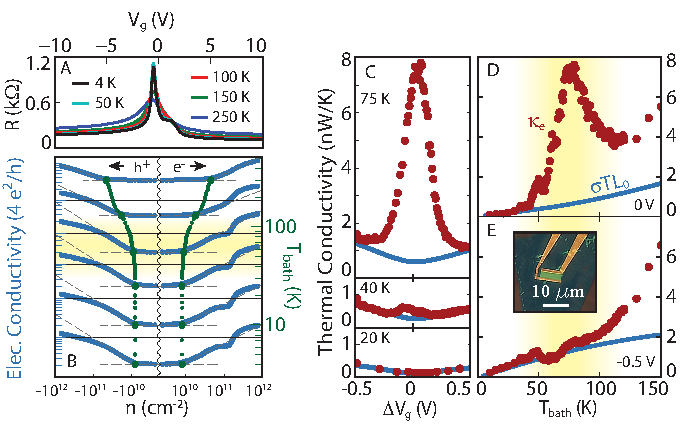
\includegraphics[width=6.25in]{Fig1.pdf}
\caption{\textbf{Temperature and density dependent electrical and thermal conductivity.} \textbf{(A)} Resistance versus gate voltage at various temperatures. \textbf{(B)} Electrical conductivity (blue) as a function of the charge density set by the back gate for different bath temperatures. The residual carrier density at the neutrality point (green) is estimated by the intersection of the minimum conductivity with a linear fit to $\log(\sigma)$ away from neutrality (dashed grey lines). Curves have been offset vertically such that the minimum density (green) aligns with the temperature axis to the right. Solid black lines correspond to $4e^2/h$. At low temperature, the minimum density is limited by disorder (charge puddles). However, above $T_{\mathrm{dis}}\sim$ 40~K, a crossover marked in the half-tone background, thermal excitations begin to dominate and the sample enters the non-degenerate regime near the neutrality point. \textbf{(C-E)} Thermal conductivity (red points) as a function of (C) gate voltage and (D-E) bath temperature compared to the Wiedemann-Franz law, $\sigma T\mathcal{L}_0$ (blue lines).  At low temperature and/or high doping ($|\mu| \gg k_{\mathrm{B}}T$), we find the WF law to hold.  This is a non-trivial check on the quality of our measurement. In the non-degenerate regime ($|\mu|<k_{\mathrm{B}}T$) the thermal conductivity is enhanced and the WF law is violated. Above $T\sim$ 100~K, electron-phonon coupling becomes appreciable and begins to dominate thermal transport at all measured gate voltages.   At this temperature, the half-tone background ends.   All data from this figure is taken from sample S2 (inset 1E).}
\label{Fig1}
\end{figure*}

Away from the CNP, graphene has a sharp Fermi surface and the standard FL phenomenology holds. By tuning the chemical potential, we may measure thermal and electrical conductivity in both the Dirac fluid (DF) and the FL in the same sample. In a FL, the relaxation of heat and charge currents is closely related as they are carried by the same quasiparticles. The Wiedemann-Franz (WF) law \cite{ashcroft} states that the electronic contribution to a metal's thermal conductivity $\kappa_{\mathrm{e}}$ is proportional to its electrical conductivity $\sigma$ and temperature $T$, such that the Lorenz ratio $\mathcal{L}$ satisfies
\begin{equation}
\label{WF}
\mathcal{L}\equiv\frac{\kappa_{\mathrm{e}}}{\sigma T}=\frac{\pi^2}{3}\left(\frac{k_{\mathrm{B}}}{e}\right)^2\equiv\mathcal{L}_0
\end{equation}
where $e$ is the electron charge, $k_{\mathrm{B}}$ is the Boltzmann constant, and $\mathcal{L}_0$ is the Sommerfeld value derived from FL theory. $\mathcal{L}_0$ depends only on fundamental constants, and not on specific details of the system such as carrier density or effective mass. As a robust prediction of FL theory, the WF law has been verified in numerous metals \cite{ashcroft}. However, in recent years, an increasing number of non-trivial violations of the WF law have been reported in strongly interacting systems such as Luttinger liquids \cite{wakeham}, metallic ferromagnets \cite{rpsmith}, heavy fermion metals \cite{tanatar}, and underdoped cuprates \cite{Hill:2001gf}, all related to the emergence of non-Fermi liquid behavior.

The WF law is expected to be violated at the CNP in a DF due to the strong Coulomb interactions between thermally excited charge carriers. An electric field drives electrons and holes in opposite directions; collisions between them introduce a frictional dissipation, resulting in a finite conductivity even in the absence of disorder \cite{muller4}. In contrast, a temperature gradient causes electrons and holes to move in the same direction inducing an energy current, which grows unimpeded by inter-particle collisions (Fig. 3C inset). The thermal conductivity is therefore limited only by the rate at which momentum is relaxed due to residual impurities.  

Realization of the Dirac fluid in graphene requires that the thermal energy be larger than the local chemical potential $\mu(\mathbf{r})$, defined at position $\mathbf{r}$: $k_{\mathrm{B}}T\gtrsim |\mu(\mathbf{r})|$. Impurities cause spatial variations in the local chemical potential, and even when the sample is globally neutral, it is locally doped to form electron-hole puddles with finite $\mu(\mathbf{r})$ \cite{sarma1, yacoby2007, crommie, xue}. Formation of the DF is further complicated by phonon scattering at high temperature which can relax momentum by creating additional inelastic scattering channels. This high temperature limit occurs when the electron-phonon scattering rate becomes comparable to the electron-electron scattering rate. These two temperatures set the experimental window in which the DF and the breakdown of the WF law can be observed.

To minimize disorder, the monolayer graphene samples used in this report are encapsulated in hexagonal boron nitride (hBN) \cite{deancr}. All devices used in this study are two-terminal to keep a well-defined temperature profile \cite{fong} with contacts fabricated using the one-dimensional edge technique \cite{wang13} in order to minimize contact resistance. We employ a back gate voltage $V_{\mathrm{g}}$ applied to the silicon substrate to tune the charge carrier density $n=n_{\mathrm{e}}-n_{\mathrm{h}}$, where $n_{\mathrm{e}}$ and $n_{\mathrm{h}}$ are the electron and hole density, respectively (see supplementary materials (SM)). All measurements are performed in a cryostat controlling the temperature $T_{\mathrm{bath}}$. Fig. 1A shows the resistance $R$ versus $V_{\mathrm{g}}$ measured at various fixed temperatures for a representative device (see SM for all samples). From this, we estimate the electrical conductivity $\sigma$ (Fig.~1B) using the known sample dimensions. At the CNP, the residual charge carrier density $n_{\mathrm{min}}$ can be estimated by extrapolating a linear fit of $\log(\sigma)$ as a function of $\log(n)$ out to the minimum conductivity \cite{couto}. At the lowest temperatures we find $n_{\mathrm{min}}$ saturates to $\sim$8$\times$10$^9~$cm$^{-2}$. We note that the extraction of $n_{min}$ by this method overestimates the charge puddle energy, consistent with previous reports \cite{deancr}. Above the disorder energy scale $T_{\mathrm{dis}}\sim$40~K, $n_{\mathrm{min}}$ increases as $T_{\mathrm{bath}}$ is raised, suggesting thermal excitations begin to dominate and the sample enters the non-degenerate regime near the CNP.

The electronic thermal conductivity is measured using high sensitivity Johnson noise thermometry (JNT) \cite{fong, crossno2}. We apply a small bias current through the sample that injects a joule heating power $P$ directly into the electronic system, inducing a small temperature difference $\Delta T\equiv T_{\mathrm{e}}-T_{\mathrm{bath}}$ between the graphene electrons and the bath. The electron temperature $T_{\mathrm{e}}$ is monitored independent of the lattice temperature through the Johnson noise power emitted at 100~MHz with a 20~MHz bandwidth defined by an LC matching network. We designed our JNT to be operated over a wide temperature range 3--300~K \cite{crossno2}. With a precision of $\sim 10$ mK, we measure small deviations of $T_{\mathrm{e}}$ from $T_{\mathrm{bath}}$, i.e. $\Delta T\ll T_{\mathrm{bath}}$. In this limit, the temperature of the graphene lattice is well thermalized to the bath \cite{fong} and our JNT setup allows us to sensitively measure the electronic cooling pathways in graphene. At low enough temperatures, electron and lattice interactions are weak \cite{crossno2, fong2}, and most of the Joule heat generated in graphene escapes via direct diffusion to the contacts (SM). As temperature increases, electron-phonon scattering becomes appreciable and thermal transport becomes limited by the electron-phonon coupling strength \cite{fong2, betz, McKitterick:2015vc}. The onset temperature of appreciable electron-phonon scattering, $T_{\mathrm{el-ph}}$, depends on the sample disorder and device geometry: $T_{\mathrm{el-ph}}\sim$ 80~K \cite{fong2, crossno2, yigen, laitinen} for our samples. Below this temperature, the electronic contribution of the thermal conductivity can be obtained from $P$ and $\Delta T$ using the device dimensions (SM).

Fig. 1C plots $\kappa_{\mathrm{e}}(V_{\mathrm{g}})$ alongside the simultaneously measured $\sigma(V_{\mathrm{g}})$ at various fixed bath temperatures. Here, for a direct quantitative comparison based on the WF law, we plot the scaled electrical conductivity as $\sigma T\mathcal{L}_0$ in the same units as $\kappa_{\mathrm{e}}$. At low temperatures, $T<T_{\mathrm{dis}}\sim$ 40~K, where the puddle induced density fluctuations dominate, we find $\kappa_{\mathrm{e}}\approx\sigma T\mathcal{L}_0$, monotonically increasing as a function of carrier density with a minimum at the neutrality point, confirming the WF law in the disordered regime. As $T$ increases ($T>T_{\mathrm{dis}}$), however, the measured $\kappa_{\mathrm{e}}$ begins to deviate from the FL theory. We note that this violation of the WF law only appears close to the CNP, with the measured thermal conductivity maximized at $n=0$ (Fig 1C). 
The deviation is the largest at  75~K, where $\kappa_{\mathrm{e}}$ is over an order of magnitude larger than the value expected for a FL.  The non-monotonicity of $\kappa_{\mathrm{e}}(T)$ is consistent with acoustic phonons relaxing momentum more efficiently than impurities as $T$ increases \cite{Lucas:2015lna}, while for $T\gtrsim 100$ K in our samples, activation of  optical phonons adds an additional electron-phonon cooling pathway \cite{crossno2}, and the measured thermal conductivity is larger than $\kappa_{\mathrm{e}}$. This non-FL behavior quickly disappears as $|n|$ increases; $\kappa_{\mathrm{e}}$ returns to the FL value and restores the WF law.   In fact, away from the CNP, the WF law holds for a wide temperature range, consistent with previous reports \cite{crossno2, yigen, fong2} (Fig. 1E).    For this FL regime, we verify the WF law up to $T \sim 80$ K. 

\begin{figure}
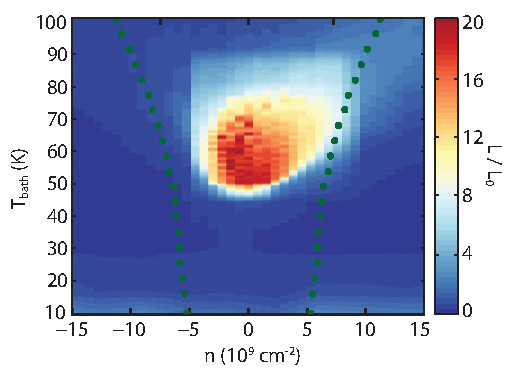
\includegraphics[width=4in]{Fig2.pdf}
\centering
\caption{\textbf{Breakdown of the Wiedemann-Franz law in the Dirac fluid regime.} The Lorenz ratio is shown as a function of the charge carrier density and bath temperature. Near the CNP and for temperatures above the disorder (charge puddle) regime but below the onset of electron-phonon coupling, the Lorenz ratio is measured to be an order of magnitude greater than the Fermi liquid value of 1 (blue). The WF law is observed to hold outside of the Dirac fluid regime.  All data from this figure is taken from sample S1.}
\label{Fig2}
\end{figure}

Our observation of the breakdown of the WF law in graphene is consistent with the emergence of the DF. Fig 2 shows the full density and temperature dependence of the experimentally measured Lorenz ratio in order to highlight the presence of the DF. The blue colored region denotes $\mathcal{L}\sim\mathcal{L}_0$, suggesting the carriers in graphene exhibit FL behavior. The WF law is violated in the DF (yellow-red) with a peak Lorenz ratio 22 times larger than $\mathcal{L}_0$. The green dotted line shows the corresponding $n_{\mathrm{min}}(T)$ for this sample; the DF is found within this regime, indicating the coexistence of thermally populated electrons and holes.    Disorder and electron-acoustic phonon scattering serve as lower and upper limits respectively on the temperature range over which the DF can be observed. \color{black}

We investigate the effect of impurities on hydrodynamic transport by comparing the results obtained from samples with varying disorder. Fig. 3A shows $n_{\mathrm{min}}$ as a function of temperature for three samples used in this study. $n_{\mathrm{min}}(T=0)$ is estimated as 5, 8, and 10$\times$10$^9~$cm$^{-2}$ in samples S1, S2, and S3, respectively. All devices show qualitatively similar Dirac fluid behavior; the largest value of $\mathcal{L}/\mathcal{L}_0$ measured in the Dirac fluid regime is 22, 12 and 3 in samples S1, S2, and S3, respectively (Fig 3B). For a direct comparison, we show $\mathcal{L}(n)$ for all three samples at the same temperature (60~K) in Fig 3C. We find that cleaner samples not only have a more pronounced peak but also a narrower density dependence, as predicted \cite{muller2, foster}.

\begin{figure}
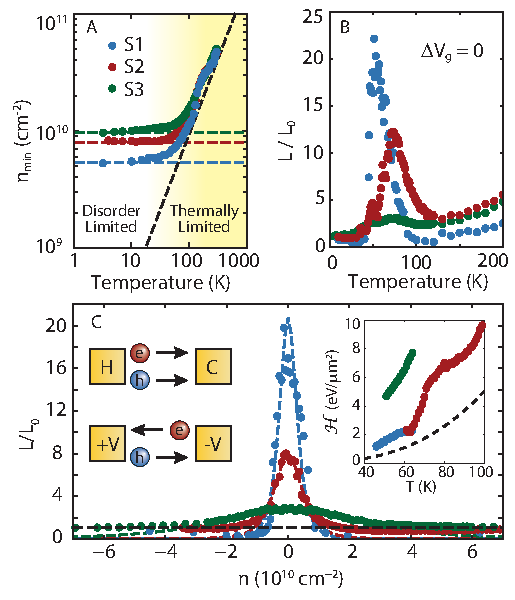
\includegraphics[width=6in]{Fig3.pdf}
\caption{\textbf{Disorder in the Dirac fluid.  (A)} Minimum carrier density as a function of temperature for all three samples.  At low temperature each sample is limited by disorder. At high temperature all samples become limited by thermal excitations.  Dashed lines are a guide to the eye. \textbf{(B)} The Lorentz ratio of all three samples as a function of bath temperature. The largest WF violation is seen in the cleanest sample. \textbf{(C)} The gate dependence of the Lorentz ratio is well fit to hydrodynamic theory of Ref. \cite{muller2,foster}. Fits of all three samples are shown at 60~K. All samples return to the Fermi liquid value (black dashed line) at high density. Inset shows the fitted enthalpy density as a function of temperature and the theoretical value in clean graphene (black dashed line). Schematic inset illustrates the difference between heat and charge current in the neutral Dirac plasma.}
\label{Fig3}
\end{figure}

More quantitative analysis of $\mathcal{L}(n)$ in our experiment can be done by employing a quasi-relativistic hydrodynamic theory of the DF incorporating the effects of weak impurity scattering \cite{hkms, muller2, foster}:
\begin{equation}
\label{Lorentz}
 \mathcal{L} =  \frac{\mathcal{L}_{\mathrm{DF}}}{\left(1+(n/n_0)^2\right)^2}
 \end{equation}
 where 
\begin{equation}
\mathcal{L}_{\mathrm{DF}} = \frac{\mathcal{H}v_{\mathrm{F}}l_{\mathrm{m}}}{T^2 \sigma_{\mathrm{min}}} \;\;\;\; \textrm{~and~} \;\;\;\; n_0^2 = \frac{\mathcal{H}\sigma_{\mathrm{min}}}{e^2v_{\mathrm{F}}l_{\mathrm{m}}}.
\end{equation}
Here $v_{\mathrm{F}}$ is the Fermi velocity in graphene, $\sigma_{\mathrm{min}}$ is the electrical conductivity at the CNP, $\mathcal{H}$ is the fluid enthalpy density, and $l_m$ is the momentum relaxation length from impurities. Two parameters in Eqn. (\ref{Lorentz}) are undetermined for any given sample: $l_m$ and  $\mathcal{H}$.  For simplicity, we assume we are well within the DF limit where $l_m$ and $\mathcal{H}$ are approximately independent of $n$. We fit Eqn. (\ref{Lorentz}) to the experimentally measured $\mathcal{L}(n)$ for all temperatures and densities in the Dirac fluid regime to obtain $l_{\mathrm{m}}$ and $\mathcal{H}$  for each sample.  Fig 3C shows three representative fits to Eqn. (\ref{Lorentz}) taken at 60 K. $l_{\mathrm{m}}$ is estimated to be 1.5, 0.6, and 0.034 $\mu$m for samples S1, S2, and S3, respectively.  For the system to be well described by hydrodynamics, $l_{\mathrm{m}}$ should be long compared to the electron-electron scattering length of $\sim$0.1 $\mu$m expected for the Dirac fluid at 60 K \cite{muller2009}.  This is consistent with the pronounced signatures of hydrodynamics in S1 and S2, but not in S3, where only a glimpse of the DF appears in this more disordered sample. We also observe in S1 that $\mathcal{L}(n)$ dips substantially below $\mathcal{L}_0$:  its minimum is $\sim \mathcal{L}_0/3$.   $\mathcal{L}<1$ is predicted to occur in Eq. (\ref{Lorentz}) for $n\gg n_0$.   Our analysis also allows us to estimate the thermodynamic quantity $\mathcal{H}(T)$ for the DF. The Fig. 3C inset shows the fitted enthalpy density as a function of temperature compared to that expected in clean graphene (dashed line) \cite{muller2009}, excluding renormalization of the Fermi velocity. In the cleanest sample $\mathcal{H}$ varies from 1.1-2.3 eV/$\mu$m$^2$ in the hydrodynamic regime.   This enthalpy density corresponds to  $\sim$ 20 meV or $\sim4k_{\mathrm{B}}T$ per charge carrier --- about a factor of 2 larger than the model calculation without disorder \cite{muller2009}.    The sharp temperature and impurity dependence observed in $\mathcal{L}$ is a prediction of these hydrodynamic models.   These effects and the magnitude of $\mathcal{L}$ are inconsistent with alternative models for WF violations, including bipolar diffusion in graphene \cite{yoshino}.  Furthermore, recent experiments report monotonic behavior in thermopower as a function of $T$ \cite{ghahari}, implying phonon drag is not responsible for the peak in $\kappa_{\mathrm{e}}$ that we observe as a function of $T$. \color{black}

To fully incorporate the effects of disorder, a hydrodynamic theory treating inhomogeneity non-perturbatively  is necessary  \cite{Lucas:2015lna, Lucas:2015sya}. The enthalpy densities reported here are larger than the theoretical estimation obtained for disorder free graphene, consistent with the picture that chemical potential fluctuations prevent the sample from reaching the Dirac point. 
While we find thermal conductivity well described by Ref.~\cite{muller2009, foster}, electrical conductivity increases slower than expected away from the CNP,  a result consistent with hydrodynamic transport in a viscous fluid with charge puddles \cite{Lucas:2015sya}.

In a hydrodynamic system, the ratio of shear viscosity $\eta$ to entropy density $s$ is an indicator of the strength of the interactions between constituent particles.   It is suggested that the DF can behave as a nearly perfect fluid \cite{muller2009}: $\eta/s$ approaches a conjecture by Kovtun-Son-Starinets: $(\eta/s)/(\hbar/k_B) \gtrsim 1/4\pi$ for a strongly interacting system \cite{Kovtun:2004de}.  A non-perturbative hydrodynamic framework can be employed to estimate $\eta$, as we discuss elsewhere \cite{Lucas:2015lna}.   A direct measurement of $\eta$ is of great interest.  


We have experimentally discovered the breakdown of the WF law and provided evidence for the hydrodynamic behavior of the Dirac fermions in graphene. This provides an experimentally realizable Dirac fluid and opens the way for future studies of strongly interacting relativistic many-body systems. Beyond a diverging thermal conductivity and an ultra-low viscosity, other peculiar phenomena are expected to arise in this plasma. The massless nature of the Dirac fermions is expected to result in a large kinematic viscosity, despite  a small shear viscosity $\eta$.   Observable hydrodynamic effects have also been predicted to extend into the FL regime \cite{vignale}.  The study of magnetotransport in the DF will lead to further tests of hydrodynamics \cite{muller2,hkms}.



\chapter{Hydrodynamic transport in the Dirac fluid}

Below we present the original text of \cite{Lucas:2015sya}.  Reprinted with permission from A. Lucas, J. Crossno, K. C. Fong, P. Kim and S. Sachdev,  ``Hydrodynamic transport in quantum critical fluids and in the Dirac fluid in graphene",  Physical Review \textbf{B93} 075426 (2016).   Copyright (2016) by the American Physical Society.

\section{Introduction}
Over a half century ago, the theory of electronic transport in ``standard" metals such as iron and copper was developed.  The key pillar of this approach is the validity of Fermi liquid theory, which states that the interacting electrons in solids form nearly free-streaming quasiparticles \cite{pines}.  At finite temperature, these quasiparticles form a weakly interacting quantum gas which is well described by quantum kinetic theory.   The transport properties of these quantum gases are by now very well understood.   A particularly important property of Fermi liquids is the Wiedemann-Franz law, which states that\footnote{Below we have assumed that the charge of the quasiparticles is $\pm e$, with $e$ the charge of the electron -- this is essentially always the case.} \begin{equation}
\mathcal{L} \equiv \frac{\kappa}{\sigma T} = \frac{\mpi^2}{3} \frac{k_{\mathrm{B}}^2}{e^2} \equiv \mathcal{L}_{\mathrm{WF}}.
\end{equation}
Here $\kappa$ is the electronic contribution to thermal conductivity, $\sigma$ is the electrical conductivity, $T$ is the temperature, and $\mathcal{L}$ is the Lorenz ratio.   Implicit in the above equation is that the dominant interactions are between impurities or phonons and quasiparticles, and in most metals this is true:  the interaction time between quasiparticles is typically $10^4$ times longer than the interaction times between quasiparticles and impurities or phonons \cite{ashcroft}.   

Also over a half century ago,  a study of the consequences of hydrodynamic behavior on correlation functions and transport in interacting quantum systems was initiated \cite{Kadanoff1963419}.    Hydrodynamics is a framework for understanding the collective motion of the quasiparticles in a solid, or any other interacting quantum or classical system, so long as the microscopic degrees of freedom reach thermal equilibrium locally.   In a solid, this interaction time must be the fastest time scale in the problem to see hydrodynamic behavior, but since quasiparticles in a Fermi liquid interact with each other only very weakly, observing hydrodynamics in electron fluids is notoriously hard.  Even in the purest metals where hydrodynamic behavior can be observed, such as in GaAs \cite{molenkamp, weber, lilly},  the resulting fluid is often a Fermi liquid.  The resulting dynamics is the fluid dynamics of (quantum) gases.  More recent theoretical work on hydrodynamics in Fermi liquids 
includes \cite{andreev2011, succiturb, tomadin, vignale, polini, levitovhydro}, and recent experimental work includes \cite{bandurin, mackenzie}.

Fermi liquid theory is known to fail in a variety of experimentally realized metals in two or more spatial dimensions -- most famous among these is the strange metal phase of the cuprate superconductors \cite{vandermarel, hussey, sk}  which does not have quasiparticle excitations.  A slightly more theoretically controlled  and better understood example  of a state of quantum matter without quasiparticles is the quasi-relativistic Dirac fluid in the semimetal graphene.   The Dirac fluid, which effectively lives in two spatial dimensions, has also been argued to be strongly interacting at experimentally achievable temperatures \cite{schmalian, muller1, muller4, andrei} due to ineffective Coulomb screening \cite{lanzara}.    Although it is separated from the Fermi liquid by a crossover, and not a (thermal) phase transition, its proximity to a (simple) zero temperature quantum critical point at charge neutrality means that the phenomenology of the Dirac fluid is expected to differ strongly from Fermi liquid theory.   Due to the high spatial dimensionality,\footnote{Quantum dynamics in one dimension,  which is often integrable, is described using very different techniques and has qualitatively distinct features.} the development of a predictive quantitative theory of these systems is notoriously hard.   A major theme in recent work has been quantum criticality \cite{Damle97,ssbook}, which opens up the possibility for borrowing powerful techniques from high energy physics,  but even in this case very little is known about experimentally relevant regime of finite temperature and density.    One of the only remaining techniques for understanding these systems is hydrodynamics, as many features of hydrodynamics are universal and model independent, and the strongly interacting quantum physics is captured entirely by the coefficients in otherwise classical differential equations.  Such fluids are quantum analogues of classical liquids such as water, which are strongly interacting (albeit with negligible quantum entanglement) insofar as they do not admit a controllable description via kinetic theory.   Furthermore, it has been shown \cite{hkms} that strongly interacting quantum critical fluids have a somewhat different hydrodynamic description than the canonical Fermi liquids described above, and this can lead to very different hydrodynamic properties,  including in transport \cite{hkms, muller1, muller4, muller2, muller2009, foster, Davison:2013txa}, as we will review in this paper.

Using novel techniques to measure thermal transport \cite{fong, fong2, crossno2},  the Dirac fluid has finally been  observed in monolayer graphene, and evidence for its hydrodynamic behavior  has emerged \cite{Crossno1058}, as we will detail.  However, existing theories of hydrodynamic transport are not consistent with the simultaneous density dependence in experimentally measured thermal and electrical conductivities.   In this paper, we improve upon the hydrodynamic theory of \cite{hkms}, describe carefully effects of finite density, and develop a non-perturbative relativistic hydrodynamic theory of transport in electron fluids near a quantum critical point.   Under certain assumptions about the equations of state of the Dirac fluid, our theory is quantitatively consistent with experimental observations.   The techniques we employ are included in the framework of \cite{Lucas:2015lna}, which developed a hydrodynamic description of transport in relativistic fluids with long wavelength disorder in the chemical potential.   \cite{Lucas:2015lna} was itself inspired by recent progress employing the AdS/CFT correspondence to understand quantum critical transport in strange metals \cite{Blake:2013owa, Davison:2013txa, Balasubramanian:2013yqa, lucas1401, Lucas:2015vna, Davison:2015bea, Blake:2015epa, Donos:2015gia,  Grozdanov:2015qia}, but as we will discuss, this theory is also well suited to describe the physics of graphene.



\subsection{Summary of Results}
The recent experiment \cite{Crossno1058} reported order-of-magnitude violations of the Wiedemann-Franz law.   The results were compared with the standard theory of hydrodynamic transport in quantum critical systems \cite{hkms}, which predicts that \begin{subequations}\label{hkmseq}\begin{align}
\sigma(n) &= \sigma_{\textsc{q}} + \frac{e^2v_{\mathrm{F}}^2n^2\tau}{\mathcal{H}}, \\
\kappa(n) &= \frac{v_{\mathrm{F}}^2\mathcal{H}\tau}{T}  \frac{\sigma_{\textsc{q}}}{\sigma(n)},
\end{align}\end{subequations}
where $e$ is the electron charge, $s$ is the entropy density, $n$ is the charge density (in units of $\mathrm{length}^{-2}$),  $\mathcal{H}$ is the enthalpy
 density,  $\tau$ is a momentum relaxation time, and $\sigma_{\textsc{q}}$ is a quantum critical effect,  whose existence is a new effect in the hydrodynamic gradient expansion of a relativistic fluid.   Note that up to $\sigma_{\textsc{q}}$,  $\sigma(n)$ is simply described by Drude physics.  The Lorenz ratio then takes the general form \begin{equation}
\mathcal{L}(n) = \frac{\mathcal{L}_{\mathrm{DF}}}{(1+(n/n_0)^2)^2},  \label{hkmsLeq}
\end{equation}
 where
\begin{subequations}\begin{align}
\mathcal{L}_{\mathrm{DF}} &= \frac{v_{\mathrm{F}}^2\mathcal{H}\tau}{T^2\sigma_{\textsc{q}}}, \\
n_0^2 &= \frac{\mathcal{H} \sigma_{\textsc{q}}}{e^2 v_{\mathrm{F}}^2 \tau}.
\end{align}\end{subequations}
$\mathcal{L}(n)$ can be parametrically larger than $\mathcal{L}_{\mathrm{WF}}$ (as $\tau\rightarrow\infty$ and $n\ll n_0$),  and much smaller ($n\gg n_0$).    Both of these predictions were observed in the recent experiment,  and fits of the measured $\mathcal{L}$ to (\ref{hkmsLeq}) were quantitatively consistent,  until large enough $n$ where Fermi liquid behavior was restored.    However, the experiment also found that the conductivity did not grow rapidly away from $n=0$ as predicted in (\ref{hkmseq}), despite a large peak in $\kappa(n)$ near $n=0$,  as we show in Figure \ref{mainfig}.   Furthermore, the theory of \cite{hkms} does not make clear predictions for the temperature dependence of $\tau$, which determines $\kappa(T)$.


\begin{figure}[t]
\centering
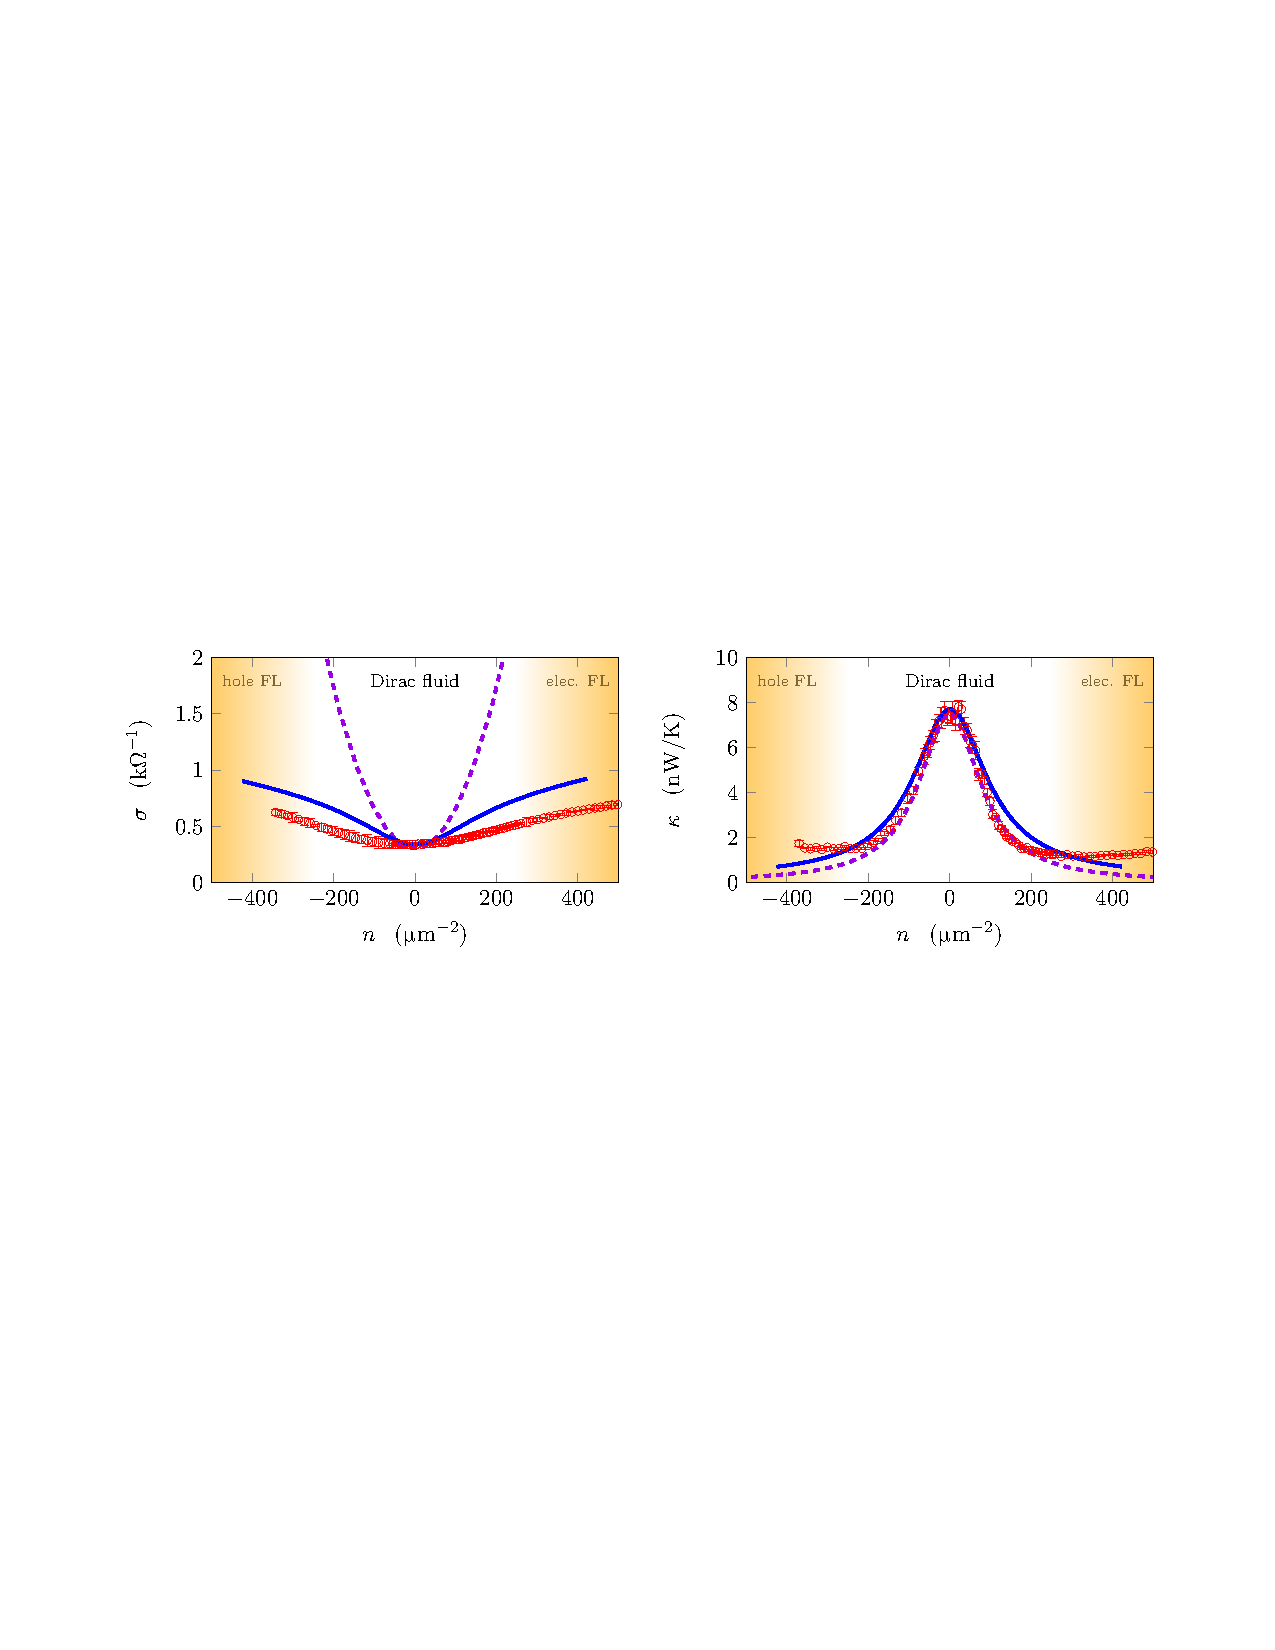
\includegraphics[width=6in]{mainfigplot.pdf}
\caption{A comparison of our hydrodynamic theory of transport with the experimental results of \cite{Crossno1058} in clean samples of graphene at $T=75$ K.   We study the electrical and thermal conductances at various charge densities $n$ near the charge neutrality point.  Experimental data is shown as circular red data markers, and numerical results of our theory, averaged over 30 disorder realizations, are shown as the solid blue line.   Our theory assumes the equations of state described in (\ref{numericmain}) with the parameters $C_0\approx 11$, $C_2\approx 9$,  $C_4\approx 200$,  $\eta_0\approx 110$, $\sigma_0\approx 1.7$,  and (\ref{numericmain2}) with $u_0 \approx 0.13$.   The yellow shaded region shows where Fermi liquid behavior is observed and the Wiedemann-Franz law is restored, and our hydrodynamic theory is not valid in or near this regime.   We also show the predictions of (\ref{hkmseq}) as dashed purple lines, and have chosen the 3 parameter fit to be optimized for $\kappa(n)$. }
\label{mainfig}
\end{figure}

\begin{figure}[t]
\centering
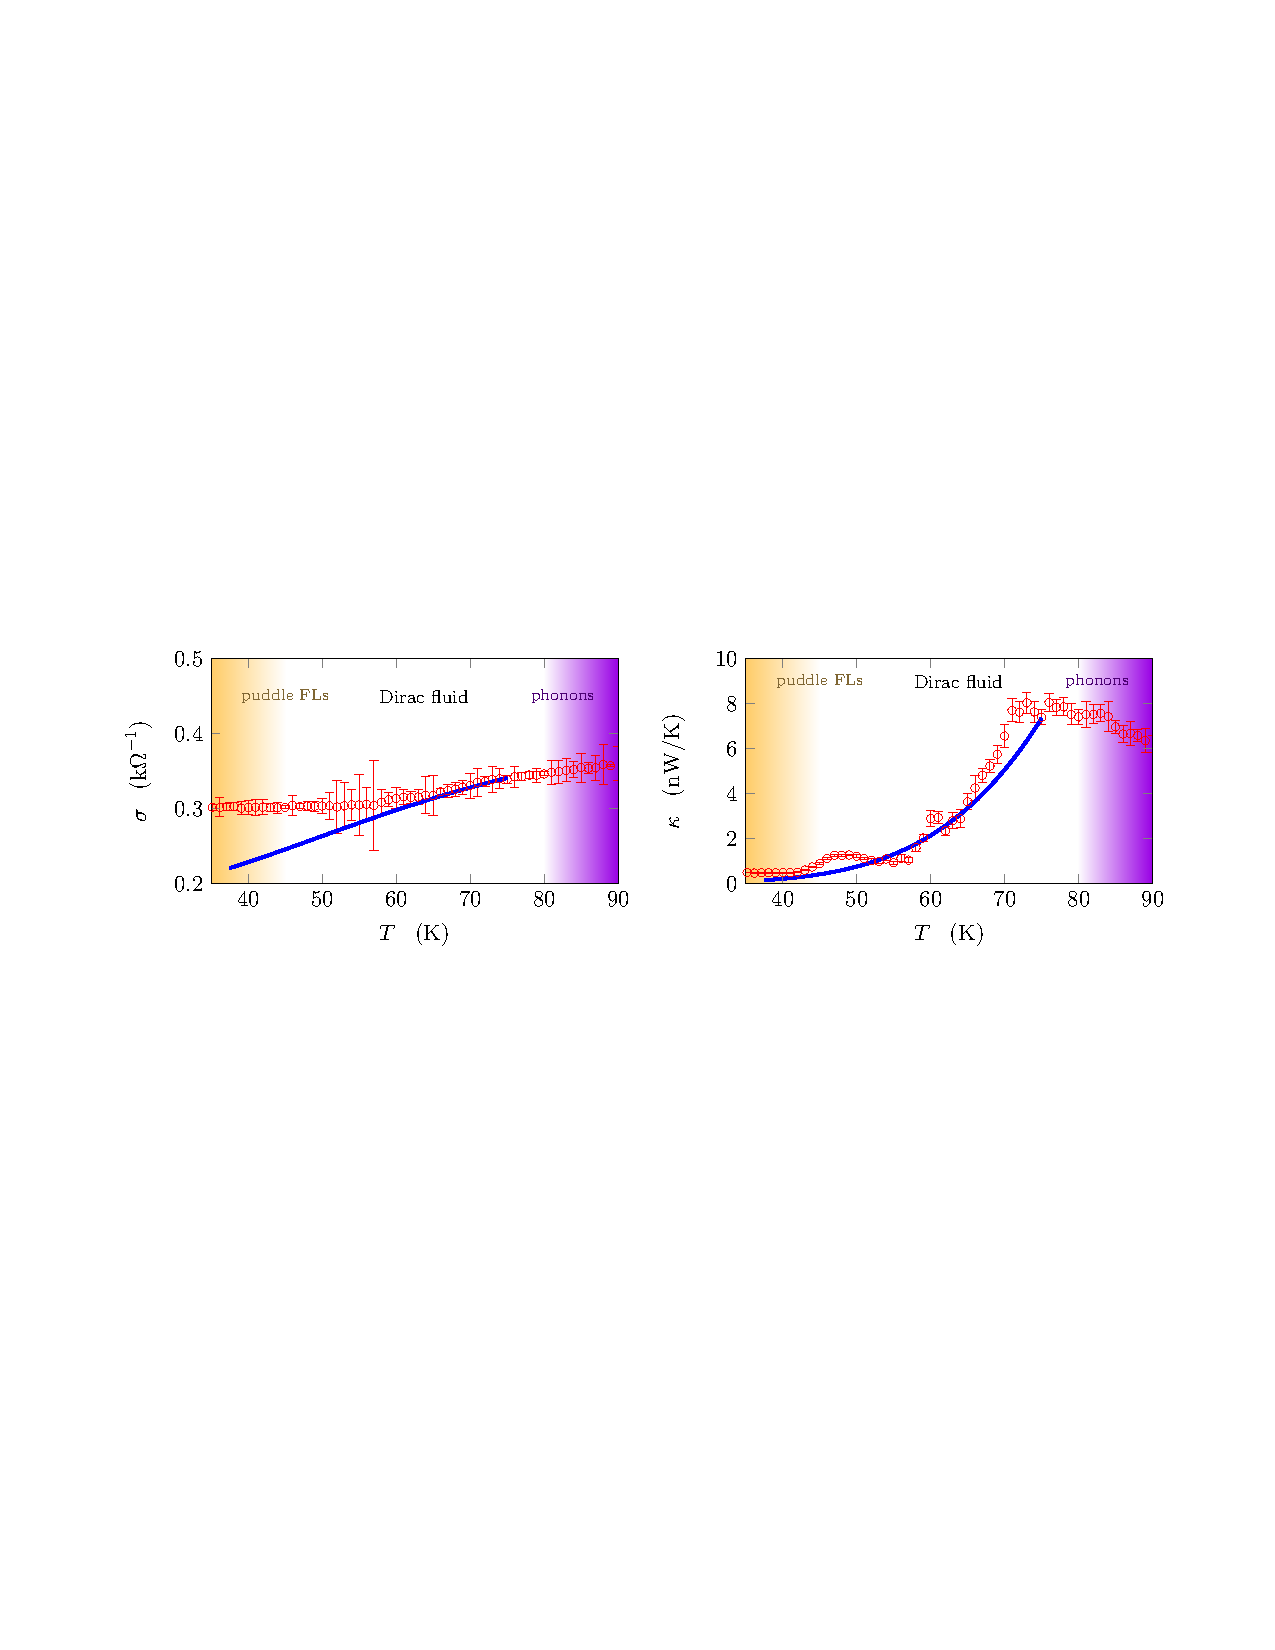
\includegraphics[width=6in]{mainfigTplot.pdf}
\caption{A comparison of our hydrodynamic theory of transport with the experimental results of \cite{Crossno1058} in clean samples of graphene at the charge neutrality point ($n=0$).  We use no new fit parameters compared to Figure \ref{mainfig}.   The yellow shaded region denotes where Fermi liquid behavior is observed; the purple shaded region denotes the likely onset of electron-phonon coupling.}
\label{mainfigT}
\end{figure}


In this paper, we argue that there are two related reasons for the breakdown of (\ref{hkmseq}).  One is that the dominant source of disorder in graphene -- fluctuations in the local charge density, commonly referred to as charge puddles \cite{yacoby2007, sarmachargepuddles, crommie, xue} --  are not perturbatively weak, and therefore a non-perturbative treatment of their effects is necessary.\footnote{See \cite{sarma1, sarma2} for a theory of electrical conductivity in charge puddle dominated graphene at low temperatures.}   The second is that the parameter $\tau$, even when it is sharply defined, is intimately related to both the viscosity and to $n$, and this $n$ dependence is neglected when performing the  fit to (\ref{hkmseq}) in Figure \ref{mainfig}.    We develop a non-perturbative hydrodynamic theory of transport which relies on neither of the above assumptions, and gives us an explicit formula for $\tau$ in the limit of weak disorder.   The key assumption for the validity of our theory is that the size of the charge puddles is comparable to or larger than the electron interaction length scale, which is about 100 nm.   Experimental evidence suggests this is  marginally true in graphene samples mounted on hexagonal boron nitride \cite{xue}, as was done in \cite{Crossno1058}.   Although we cannot analytically solve our theory non-perturbatively, we perform numerical computations of the transport coefficients in disordered fluids, and compare the results to the experimental data in Figure \ref{mainfig}.  Our simultaneous fit to $\kappa(n)$ and $\sigma(n)$ shows improved quantitative agreement with both sets of data in the Dirac fluid regime.    We further compare in Figure \ref{mainfigT} the temperature dependence of $\kappa$ and $\sigma$ between our numerics and the experiment, using no new fitting parameters, and find satisfactory quantitative agreement in the Dirac fluid regime.  

\begin{figure}[t]
\centering
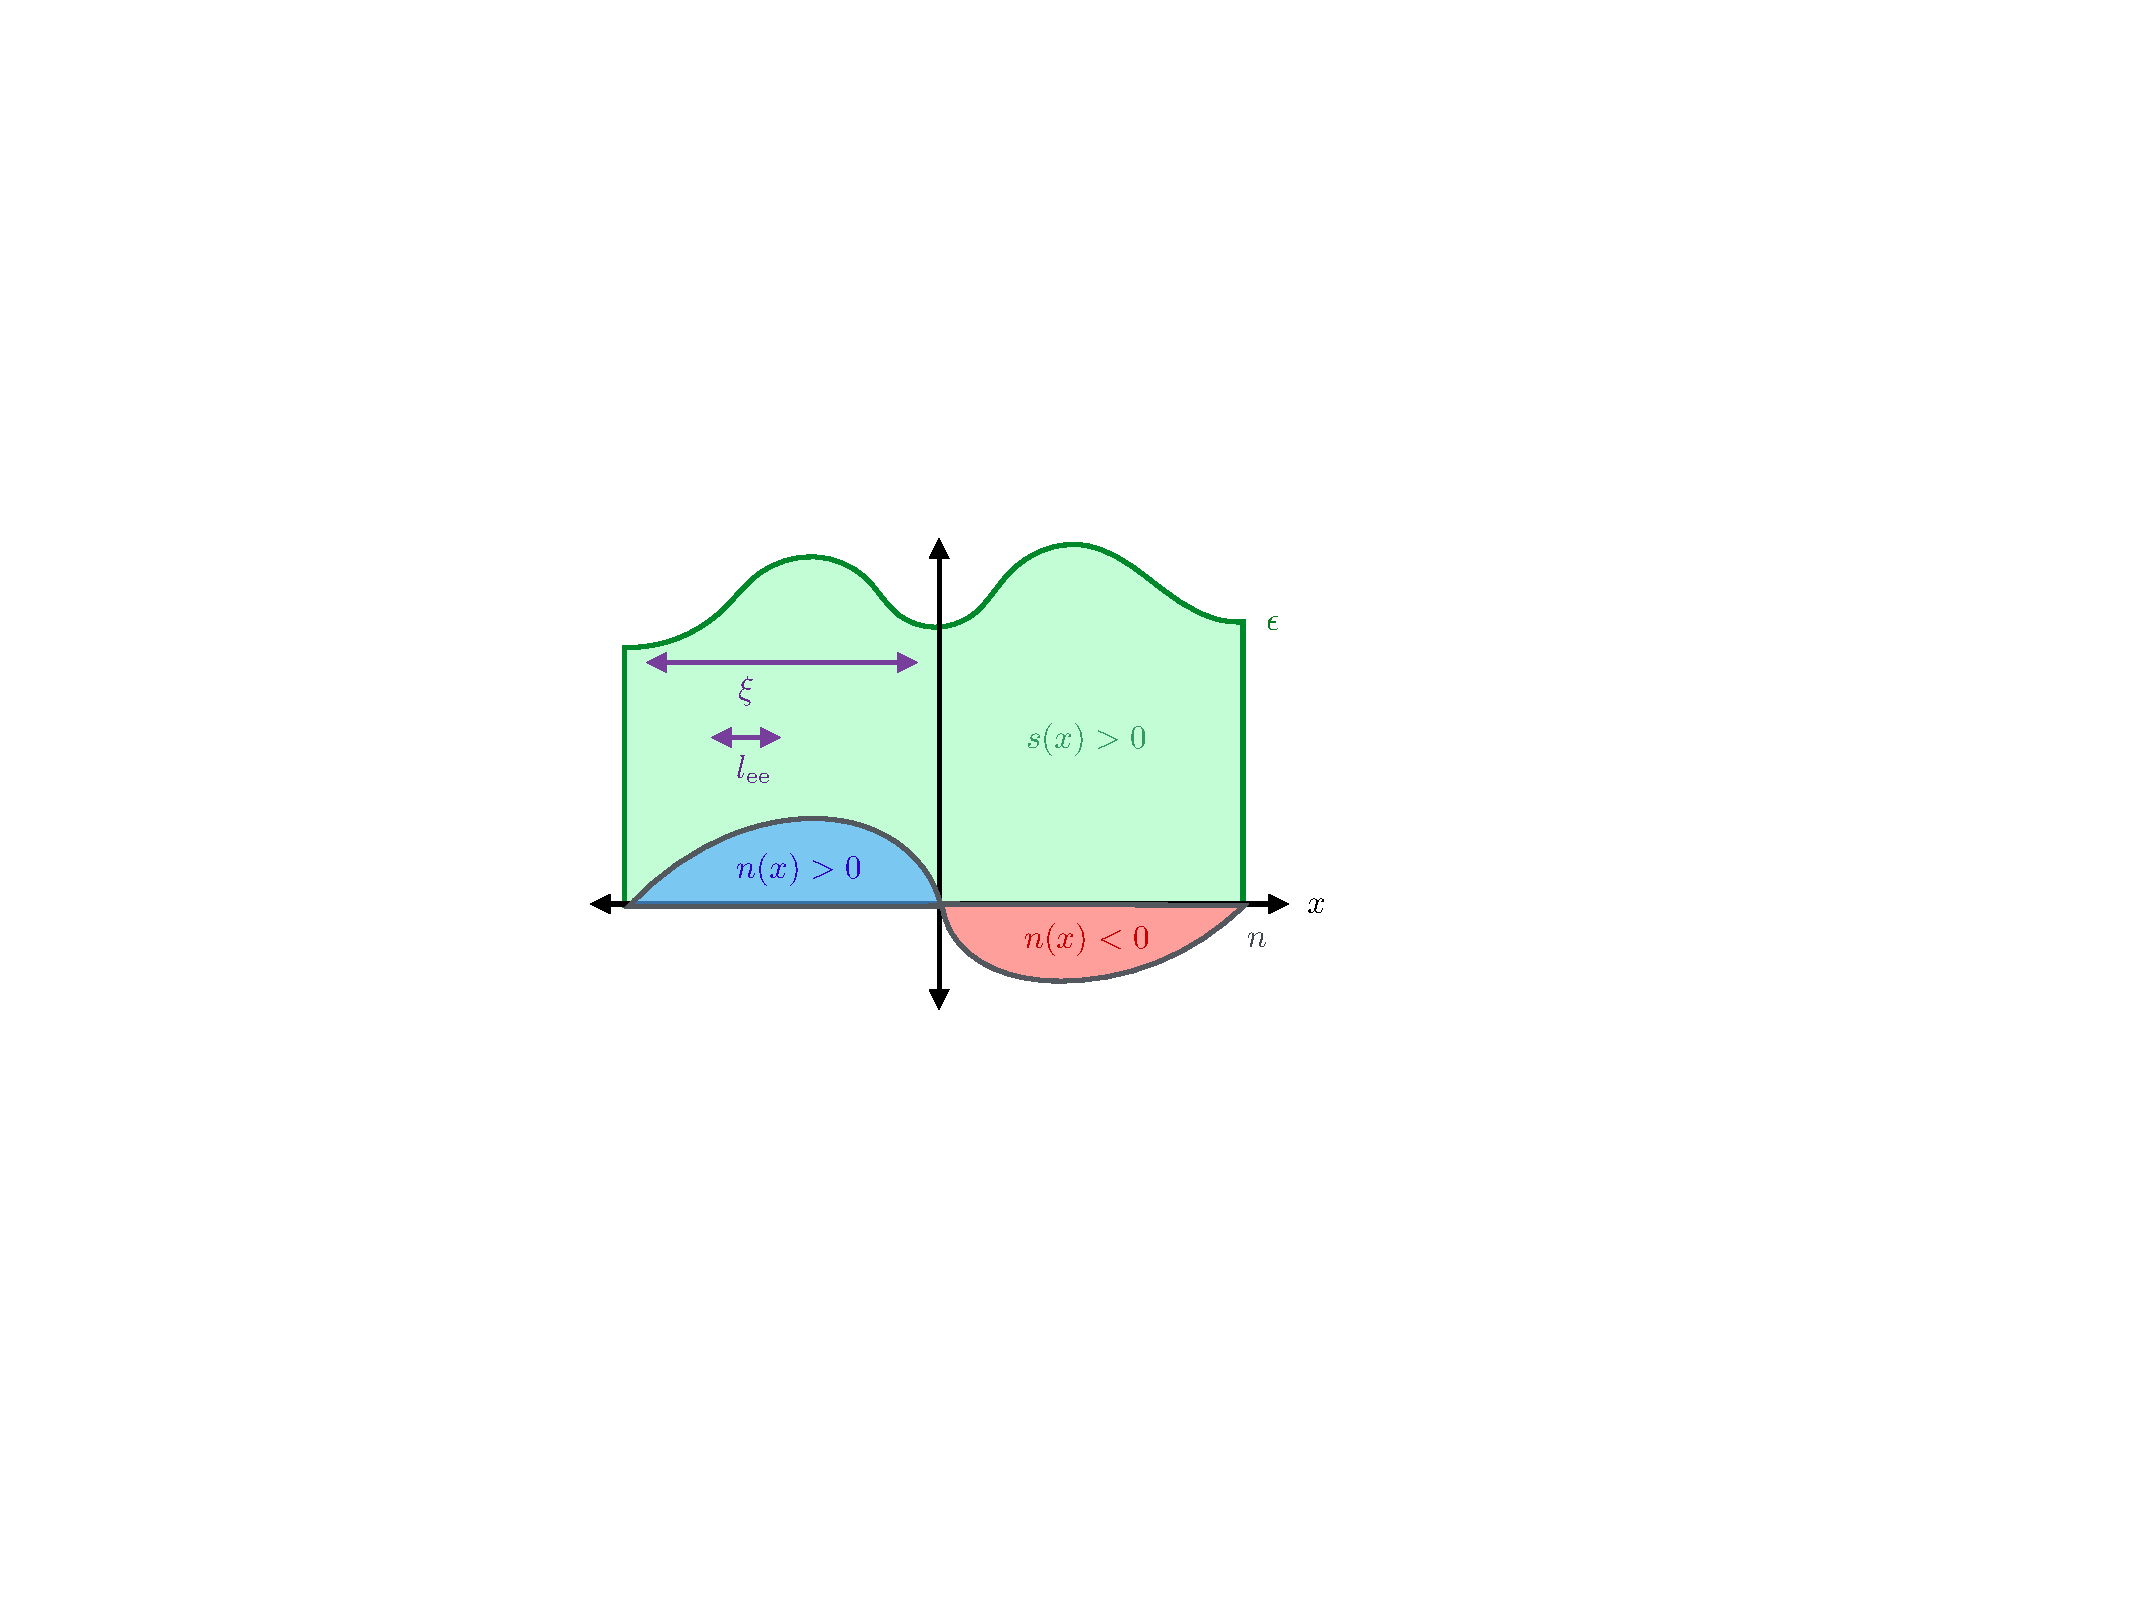
\includegraphics[width=3.3in]{hydrofig.pdf}
\caption{A cartoon of a nearly quantum critical fluid where our hydrodynamic description of transport is sensible.   The local chemical potential $\mu(\mathbf{x})$ always obeys $|\mu| \ll k_{\mathrm{B}}T$,  and so the entropy density $s/k_{\mathrm{B}}$ is much larger than the charge density $|n|$;  both electrons and holes are everywhere excited, and the energy density $\epsilon$ does not fluctuate as much relative to the mean.  Near charge neutrality the local charge density flips sign repeatedly.   The correlation length of disorder $\xi$ is much larger than $l_{\mathrm{ee}}$, the electron-electron interaction length.}
\label{hydrofig}
\end{figure}

Figure \ref{hydrofig} shows a cartoon of the regime of validity of our hydrodynamic theory.   The fact that the charge puddles may be substantial, while the entropy and energy densities are much more constant,  helps to explain why the perturbative description of transport is much better for $\kappa$ than $\sigma$,  as the perturbative approach works well in a nearly homogeneous fluid.  In coming years the quality of graphene samples will improve, and the charge puddle size may grow larger than 100 nm, allowing us to observe the clean hydrodynamic limit described by (\ref{hkmseq}).   As present day samples are just clean enough to observe hydrodynamics, our determination of the equations of state should be understood as preliminary.



%Interestingly, our hydrodynamic theory turns out to be quite sensitive to the viscosity of the underlying Dirac fluid.  This effect, which can be seen perturbatively,  was not taken into account in \cite{hkms}, as in this paper the disorder was assumed to be driven by scalar operators and not by charge puddles.   As pointed out in Figure \ref{mainfig},  we obtain a first  estimate of the viscosity of the Dirac fluid directly from experiment.

Although the focus of this paper is on the Dirac fluid in graphene, this is because of the experimental motivation for this work.   Our theory has broader validity, and we will introduce it in the more general context of transport in a disordered electronic fluid near a quantum critical point with manifest Lorentz invariance, with the microscopic Fermi velocity $v_{\mathrm{F}}$ playing the role of the speed of light.  The Dirac fluid is not strictly Lorentz invariant, but we will justify the validity of our approach even in this system.   While the Dirac fluid in graphene is currently the only experimentally realized strongly interacting condensed matter system with evidence for electronic hydrodynamics \cite{Crossno1058},  in the future surface states in topological insulators in three spatial dimensions  may host strongly interacting electron fluids \cite{galitski}.  Strongly interacting three dimensional materials including Weyl semimetals \cite{soljacic, syxu, bqlv} may also give rise to novel phenomena relevant for transport \cite{nielsen, spivakson}.

\subsection{Outline}
The outline of this paper is as follows.  We briefly review the definitions of transport coefficients in Section \ref{sectransco}.   In Section \ref{sechydro} we develop a theory of hydrodynamic transport in the electron fluid, assuming that it is Lorentz invariant.  We discuss the peculiar case of the Dirac fluid in graphene in Section \ref{secgraphene}, and argue that deviations from Lorentz invariance are small.   We describe the results of our numerical simulations of this theory in Section \ref{secnum}, and directly compare our simulations with recent experimental data from graphene \cite{Crossno1058}.  The experimentally relevant effects of phonons are qualitatively described in Section \ref{secphonon}.  We conclude the paper with a discussion of future experimental directions.   Appendices contain technical details of our theory.

In this paper we use index notation for vectors and tensors.  Latin indices $ij\cdots$ run over spatial coordinates $x$ and $y$;  Greek indices $\mu\nu\cdots$ run over time $t$ as well.   We will denote the time-like coordinate of $A^\mu$ as $A^t$.  Indices are raised and lowered with the Minkowski metric $\eta^{\mu\nu} \equiv \mathrm{diag}(-1,1,1)$.  The Einstein summation convention is always employed.

\section{Transport Coefficients}\label{sectransco}
Let us begin by defining the thermoelectric response coefficients of interest in this paper.   Suppose that we drive our fluid by a spatially uniform, externally applied, electric field $ E_i$ (formally, an electrochemical potential gradient), and a temperature gradient $-\partial_i T$.  We will refer to $-\partial_j T$ as $T\zeta_j$, with $\zeta_j = -T^{-1}\partial_j T$, for technical reasons later.   As is standard in linear response theory, we decompose these perturbations into various frequencies, and focus on the response at a single frequency $\omega$.   Time translation invariance implies that the (uniformly) spatially averaged charge current $\langle  J_i \rangle$ and the spatially averaged heat current $\langle  Q_i \rangle$ are also periodic in time of frequency $\omega$, and are related to $ E_i$ and $ \zeta_i$ by the thermoelectric transport coefficients: \begin{equation}
\left( \begin{array}{c} \langle  J_i \rangle  \\ \langle  Q_i\rangle \end{array}\right) \mathrm{e}^{-\mathrm{i}\omega t} =  \left( \begin{array}{cc} \sigma_{ij}(\omega)   &\  T\alpha_{ij}(\omega) \\  T\bar\alpha_{ij}(\omega)   &\ T\bar\kappa_{ij}(\omega)  \end{array}\right)\left( \begin{array}{c}  E_j \\  \zeta_j  \end{array}\right) \mathrm{e}^{-\mathrm{i}\omega t}.   \label{transeq}
\end{equation}
 In a typical disordered system, we expect that $\sigma_{ij}$, $\alpha_{ij}$, $\bar\alpha_{ij}$ and $\bar\kappa_{ij}$ are all proportional to $\mdelta_{ij}$.   In our numerics, finite size effects introduce some anisotropy; our theory is valid in this more general scenario.

In fact, (\ref{transeq}) is somewhat subtle.   Implicit in the definitions of the transport coefficients are a set of boundary conditions.   In the definitions in (\ref{transeq}), we have assumed that we tune $E_i$ and $ \zeta_i$, and then measure $ J_i$ and $Q_i$.   However, usually in experiments one fixes $J_i$, as electronic measurements are far easier to control.  One then can fix either $E_i$ or $\zeta_i$. So while it is straightforward to measure $\sigma_{ij}$ by setting $\zeta_i=0$,  one measures not $\bar{\kappa}_{ij}$ but instead $\kappa_{ij}$, defined as \begin{equation}
\left.\langle  Q_i\rangle\right|_{\langle  J_i\rangle = 0} = T\kappa_{ij} \zeta_j.
\end{equation}Straightforward manipulations give that $\sigma_{ij}E_j = -T\alpha_{ij}\zeta_j$, and therefore that\begin{equation}
\kappa_{ij} = \bar\kappa_{ij} - T\bar\alpha_{ik}\sigma^{-1}_{kl}\alpha_{lj}.
\end{equation}
These definitions are general and independent of our hydrodynamic theory.




\section{Relativistic Hydrodynamics}\label{sechydro}
We now develop a theory of relativistic hydrodynamics of the electronic plasma in a disordered metal, where the disorder is introduced by a spatially dependent chemical potential $\mu_0(\mathbf{x})$.    So long as the length scale $\xi \sim |\mu_0|/ |\partial_x \mu_0|$ over which this function varies is much larger than the electron-electron scattering length $l_{\mathrm{ee}} \sim \hbar v_{\mathrm{F}} /k_{\mathrm{B}}T$, it is sensible to treat the fluid as locally homogeneous, with parameters such as energy density and viscosity locally being functions of $\mu_0$ alone.  This external chemical potential acts as an external source of energy and momentum for the electronic plasma, and can be sourced by lattice defects or impurities, either in the (semi)metal itself, or in the substrate it is placed on, for two-dimensional materials such as graphene \cite{yacoby2007, xue}.   Our theory here is  analogous to \cite{Lucas:2015lna}, and similar to the earlier work \cite{andreev2011} in non-relativistic fluids.   However, \cite{Lucas:2015lna} focused mostly on the mathematical consequences of relativistic hydrodynamics, particularly in regards to holographic models.   Our focus here is on practical consequences in realistic quantum critical fluids where $\mu \ll k_{\mathrm{B}}T$, and where the equations of state are tightly constrained by scale invariance (see Appendix \ref{appthermo}).

Previous theories of hydrodynamic transport assumed that disorder was parametrically weak, and so momentum is a nearly conserved quantity \cite{hkms, muller1}.    Such theories can be shown to be a perturbative limit of the more general approach that we advocate below: see \cite{Lucas:2015lna} and Appendix \ref{appmom}.    However, near the charge-neutrality point, non-perturbative effects can become important \cite{Lucas:2015lna}.  Since this is the regime where \cite{Crossno1058} observed evidence for hydrodynamic behavior, it is necessary to treat transport in the charge-neutral fluid carefully and to study non-perturbative physics.   We begin with a general discussion of the equations of state of a relativistic plasma, and then outline our non-perturbative hydrodynamic description of  transport.

Though our focus in this paper is on the case of two spatial dimensions, it is straightforward to generalize our theory to higher dimensions.


\subsection{Hydrodynamic Equations}
Let us review the structure of relativistic hydrodynamics, which was derived carefully in \cite{hkms}.  Hydrodynamics is a general framework which describes the relaxation of an ergodic and locally thermalizing (classical or quantum) system  to global thermal equilibrium, or as close to global equilibrium as boundary conditions or external sourcing allow.
%\footnote{By local thermal equilibrium, we mean that the product of correlation functions of local operators $\mathcal{O}_i$, such as the charge or energy density, can be expressed as $\mathrm{tr}[\mathcal{O}_1\cdots\mathcal{O}_n \rho]$ with the density matrix given by $\rho = \exp[T^{-1} \int \mathrm{d}^2\mathbf{x} (u_\mu(\mathbf{x})\mathcal{P}^\mu(\mathbf{x}) + \mu(\mathbf{x}) u^\mu(\mathbf{x}) \mathcal{J}^\mu(\mathbf{x}))]$,  with $\mathcal{P}^\mu$ the local energy-momentum density,  and $\mathcal{J}^\mu$ the local charge current.}
The assumption of local thermalization implies that the only quantities with dynamics on long time scales (compared to the local thermalization time $l_{\mathrm{ee}}/v_{\mathrm{F}}$)  are quantities that are globally conserved, up to external sources.    In a typical theory, these will be charge, energy and momentum, and we will assume this to be the case for graphene as well.   
%\cite{} argue that the electron and hole fluids recombine on a slow enough time scale that the electron and hole densities must be separate hydrodynamic degrees of freedom, and our framework can be extended to account for this.   
Hydrodynamics is a systematic way to truncate equations of motion for the local charge density $n(x)$,   energy density $\epsilon(x)$ and momentum density $\Pi_i(x)$, by treating the perturbative parameter as $l_{\mathrm{ee}} \partial_\mu$.    In fact, it is typical to instead study the dynamics of the thermodynamic conjugate variables: chemical potential $\mu(x)$, temperature $T(x)$ and relativistic velocity $u^\mu(x)$, respectively.  $u^\mu$ is subject to the usual constraint $u_\mu u^\mu = -v_{\mathrm{F}}^2$.

Note that throughout this paper, ``charge density" $n$ refers to the number density of electrons, minus the number density of holes:  $n=n_{\mathrm{elec}} - n_{\mathrm{hole}}$.   Thus, there are no factors of $e$ in the definition of $n$, or chemical potential $\mu$.\footnote{Therefore $[n] = [\text{length}]^{-d}$ and $[\mu]=[\text{energy}]$.}

The equations of motion of hydrodynamics are the local conservation laws, up to external sources.  We apply an external chemical potential $\mu_0$ via an external electromagnetic field $A_{\mathrm{ext}}^t = -\mu_0(\mathbf{x})/e$, $A^i_{\mathrm{ext}}=0$.   We employ relativistic notation with $v_{\mathrm{F}}=1$ temporarily.  The equations of hydrodynamics are\begin{subequations}\label{hydroeq}\begin{align}
\partial_\mu T^{\mu\nu} &= e F^{\mu\nu}_{\mathrm{ext}} J_\nu, \\
\partial_\mu J^\mu &= 0,
\end{align}\end{subequations}where $F^{ti}_{\mathrm{ext}} = -F^{it}_{\mathrm{ext}} = \partial_i \mu_0$ are the only non-vanishing components, $T^{\mu\nu}$ represents the expectation value of the local stress-energy density,  and $J^\mu$ the expectation value of the local charge density.     $T^{\mu\nu}$ and $J^\mu$ must be expressed in terms of $\mu$, $T$ and $u^\mu$ in order to obtain a closed set of equations.   One can show that there is a static solution to the hydrodynamic equations with $u^\mu = (1,0,0)$, $T=T_0=\text{constant}$, and $\mu(\mathbf{x})=\mu_0(\mathbf{x})$ \cite{Lucas:2015lna}.   Recall that $\mu_0(\mathbf{x})$ is slowly varying on the length scale $\xi$.  We will take this solution as the background state of our fluid.

%In $d=2$, we can also apply a uniform background magnetic field $B$ which breaks parity but not isotropy.   This is done by adding $A^y_{\mathrm{ext}} = Bx$, for example.   The static solution identified above is not altered by the presence of the magnetic field, although the equations of state may be.

Hydrodynamics is a perturbative expansion of (\ref{hydroeq}), where the perturbative expansion parameter is the number of derivatives of space and time.   At zeroth order, the equations of state are simply that $T^{\mu\nu}$ and $J^\mu$ are given by the  thermodynamic  relations we derived above:  \begin{subequations}\begin{align}
T^{\mu\nu} &=  (\epsilon + P)u^\mu u^\nu + P \eta^{\mu\nu}, \\
J^\mu &=  n u^\mu,
\end{align}\end{subequations} with $\epsilon$ the energy density and $P$ the pressure.   In the fluid's rest frame,  $T^{tt}=\epsilon$, $T^{ij} = P\mdelta^{ij}$, and $J^t=n$, with all other components vanishing.  At first order, \cite{hkms} showed that the most general first derivative corrections to $T^{\mu\nu}$ and $J^\mu$ consistent with symmetries and the local second law of thermodynamics are \begin{subequations}\begin{align}
T^{\mu\nu} &= (\epsilon +P )u^\mu u^\nu + P\eta^{\mu\nu}-2\mathcal{P}^{\mu\rho}\mathcal{P}^{\nu\sigma}\eta \partial_{(\rho} u_{\sigma)} - \mathcal{P}^{\mu\nu}\left(\zeta-\eta\right)\partial_\rho u^\rho   , \\
J^\mu &=  n u^\mu - \frac{\sigma_{\textsc{q}}}{e^2} \left(\eta^{\mu\nu}+u^\mu u^\nu\right)\left(\partial_\nu \mu - \frac{\mu}{T}\partial_\nu T - eF_{\nu\rho,\text{ext}}u^\rho\right),
\end{align}\end{subequations}
with $\eta,\zeta,\sigma_{\textsc{q}} >0$, and $\mathcal{P}^{\mu\nu} = \eta^{\mu\nu} + u^\mu u^\nu$.    Here $\eta$ and $\zeta$ are the shear and bulk viscosity respectively, and $\sigma_{\textsc{q}}$ is a ``quantum critical'' conductivity \cite{hkms}.
  Note that the external electromagnetic fields show up in the hydrodynamic gradient expansion in the charge current;  this happens because the charged fluid is sensitive only to the gradient in the total electrochemical potential \cite{pines}.  We allow for $P$, $n$, $\eta$, $\zeta$ and $\sigma_{\textsc{q}}$ to all be position-dependent, with their position dependence related to $\mu_{\mathrm{ext}}$, as we will describe shortly in more detail.   

It has long been appreciated \cite{hkms} that $\sigma_{\textsc{q}}$ plays a fundamental role in hydrodynamic transport near quantum critical points.   More recently \cite{Davison:2013txa} argued that $\eta$ could play a role in transport.   We will carefully detail how $\eta$ affects transport in this paper, analytically and numerically.

In our extension of this theory to graphene, we will also allow for Coulomb interactions of the fluid to be substantial enough to enter the hydrodynamic equations.  However, this should only alter the equations of state, as well as add a further contribution to $F_{\mu\nu,\mathrm{ext}}$ \cite{muller1}, and we will detail this in the subsequent section.   The constraints imposed on hydrodynamics from local positivity of entropy production \cite{hkms} are unchanged in the presence of Coulomb interactions, which are entirely accounted for via a modified $F_{\mathrm{ext}}^{\mu\nu}$.

It is sufficient in our calculation of $\sigma$, $\alpha$ and $\kappa$ to simplify $T^{\mu\nu}$ and $J^\mu$ and retain only the terms linear in velocity.   One finds, in $d=2$: \begin{subequations}\label{smallvhyd}\begin{align}
T^{ti} &= (\epsilon+P) v^i, \\
T^{ij} &= P\mdelta^{ij} - \eta \left(\partial^i v^j + \partial^j v^i\right) - (\zeta-\eta)\mdelta^{ij} \partial_k v^k, \\
J^i &= nv^i - \frac{\sigma_{\textsc{q}}}{e^2} \left(\partial_i (\mu - \mu_0)  - \frac{\mu}{T}\partial_i T \right).
\end{align}
\end{subequations}
We stress the novel role of $\sigma_{\textsc{q}}$, a new dissipative transport coefficient in a relativistic fluid, without a direct analogue in the canonical non-relativistic fluid.   This term is related to the underlying thermally excited electron-hole plasma, and the fact that electrons and holes can move in opposite directions under an applied electric field, contributing a net electric current.\footnote{It is qualitatively similar to the bipolar diffusion effect \cite{goldsmid, yoshino} -- however, in hydrodynamics the quasiparticle lifetimes are limited by $\hbar/k_{\mathrm{B}}T$, whereas in the bipolar diffusion effect these lifetimes are parametrically long, as in a Fermi liquid. \par}  There is no microscopic thermal conductivity -- instead, all microscopic dissipation related to electric and thermal gradients is controlled by $\sigma_{\textsc{q}}$.  


\subsection{Hydrodynamic Theory of Transport}
We are now ready to detail our hydrodynamic calculation of the transport coefficients defined in Section \ref{sectransco}.   We place our fluid in a box of length $L$ in each direction, with periodic boundary conditions on the fluid in every direction.   We then apply a constant background  $E_i$ and $\zeta_i$.\footnote{The application of a constant $\zeta_j$ on a periodic space is the reason why we cannot talk about driving the system with a constant temperature gradient, since the temperature is a periodic function in space.  One can formally implement $\zeta_i$ through deformations of the spacetime metric and external gauge fields \cite{Hartnoll:2009sz}.}  The static solution above is no longer a solution to the hydrodynamic equations of motion, sourced by these gradients.   Now, we generically expect to excite both a spatial electric current $J^i$, and a spatial heat current \begin{equation}\label{heatdef}
Q^i \equiv T^{ti} - \mu J^i.
\end{equation}
We can expand out $J^i$ and $Q^i$ locally as a Taylor series in $E_i$ and $\zeta_i$.   The transport coefficients in Section \ref{sectransco} are defined by retaining only the linear terms in $E_i$ and $\zeta_i$, and spatially averaging over the local charge and heat currents.   It is  sufficient to perform a linear response calculation about our previously identified static solution:
\begin{subequations}\begin{align}
\mu &\approx \mu_0(\mathbf{x}) + \mdelta \mu(\mathbf{x}) \mathrm{e}^{-\mathrm{i}\omega t},  \\
T &\approx T_0 + \mdelta T(\mathbf{x}) \mathrm{e}^{-\mathrm{i}\omega t}, \\
u^t &\approx 1, \\
u^i &\approx \mdelta v^i (\mathbf{x}) \mathrm{e}^{-\mathrm{i}\omega t},
\end{align}\end{subequations}
and then solve the linearized hydrodynamic equations -- this is equivalent to only keeping terms linear in $E_i$ and $\zeta_i$ in the full solution.   For ease of notation, we drop the ``$\mdelta$" in  front of the linear response perturbations in the remainder of the paper, but one should keep in mind that $\mu(\mathbf{x})$, $T(\mathbf{x})$, and $v^i$ are henceforth perturbatively small quantities.

Following \cite{Lucas:2015lna}, the linearized hydrodynamic equations (\ref{hydroeq}) can be shown to take the following form:\footnote{In this equation, derivatives act on all fields to the right, so $\partial_x \eta \partial_x v^x$ should be read as $\partial_x (\eta \partial_x v^x)$.} \begin{align}
 &\left(\begin{array}{ccc} - e^{-2}\partial_i \sigma_{\textsc{q}} \partial_i  &\  e^{-2}T_0^{-1} \partial_i \mu_0\sigma_{\textsc{q}} \partial_i  &\ \partial_j n   \\ e^{-2} \partial_i \mu_0\sigma_{\textsc{q}} \partial_i  &\ -e^{-2} T^{-1}_0\partial_i \mu_0^2\sigma_{\textsc{q}} \partial_i  &\ T_0\partial_j s  \\ n\partial_i   &\ s\partial_i  &\  - \partial_i (\zeta-\eta)\partial_j  - \partial_i \eta \partial_j - \partial_j \eta \partial_i  \end{array}\right)  \left(\begin{array}{c} \mu \\ T \\ v_j\end{array}\right) \notag \\
&\;\;\;\;\;\;\;\;\;\;\;  = \left(\begin{array}{c} -e^{-1}\partial_i \sigma_{\textsc{q}} (E_i - \mu_0 \zeta_i/e) \\ e^{-1} \partial_i \sigma_{\textsc{q}}  \mu_0 (E_i - \mu_0 \zeta_i/e) \\ en E_i + T_0 s\zeta_i \end{array}\right)  \label{bigeq}
\end{align}
Here \begin{equation}
s = \frac{\epsilon+P - \mu_0 n}{T_0}
\end{equation}is the entropy density of the background fluid.   $s$ and $n$ are not independent, and are related by thermodynamic Maxwell relations:  see Appendix \ref{appthermo}.   We have also employed \begin{equation}
\partial_i P =  n \partial_i \mu + s\partial_i T. 
\end{equation}
In particular, $s$ and $n$ are position dependent functions whose position dependence is entirely determined by the local chemical potential:  $s(\mathbf{x}) = s(T_0,\mu_0(\mathbf{x}))$, and similarly for $n$, $\eta$, and all other coefficients in the hydrodynamic equations.   The proper boundary conditions to impose on $\mu$, $T$ and $v_j$ are periodicity.   This forms a well-posed elliptic partial differential equation and can be numerically solved: see Appendix \ref{appfin}.   Combining (\ref{smallvhyd}) and (\ref{heatdef}), along with $\mu$, $T$ and $v^i$ as found from solving the linear system (\ref{bigeq}), we obtain $J_i(E_j,\zeta_j)$ and $Q_i(E_j,\zeta_j)$.  Spatially averaging these quantities and employing (\ref{transeq}), we obtain $\sigma_{ij}$,$\alpha_{ij}$ and $\bar\kappa_{ij}$. 

We cannot exactly compute these transport coefficients in general.   However, one can prove \cite{Lucas:2015lna} that Onsager reciprocity holds.  This is a non-trivial consistency check on the validity of our approach.   Furthermore, there exist scaling symmetries combining re-scalings of $\mu$, $T$ and $v_i$, as well as the equations of state;  these are listed in Appendix \ref{apprescale}.   These are helpful when we fit this theory to the data of \cite{Crossno1058}.   These scaling symmetries are also present in the theory of \cite{hkms}, with the exception of a further scaling symmetry which only affects the viscosity and the length scale of disorder in this theory.

In the limit where \begin{equation}
\mu_0 = \bar\mu_0 +  u \hat\mu(\mathbf{x}),  \label{pertlimit}
\end{equation} 
with $\hat\mu$ an O(1) function but $u \ll \bar\mu_0$, the transport coefficients may be perturbatively calculated analytically, and for $\mu \ll k_{\mathrm{B}}T$,  we find that \begin{subequations}\label{drudeeq}\begin{align}
\sigma &\approx \frac{e^2v_{\mathrm{F}}^2n^2\tau}{\epsilon+P}, \\
\alpha &\approx \frac{ev_{\mathrm{F}}^2ns\tau}{\epsilon+P}, \\
\bar\kappa &\approx \frac{v_{\mathrm{F}}^2Ts^2\tau}{\epsilon+P},
\end{align}\end{subequations} 
and we find an analytical expression for $\tau$ with the following approximate form near the Dirac point: \begin{equation}
\frac{1}{\tau} \approx \frac{v_{\mathrm{F}}^2 u^2}{2} \left(\frac{\partial n}{\partial \mu}\right)^2 \left[\frac{e^2 }{\sigma_{\textsc{q}}(\epsilon+P)} + \frac{\eta+\zeta}{\xi^2} \frac{4\mu^2}{(\epsilon+P)^3} \right].  \label{taumain}
\end{equation}  Details of this calculation and a more precise (and complicated) formula are given in Appendix \ref{appmom}.    The requirement that we are ``far" from the Dirac point is that $\sigma_{\textsc{q}} \ll e^2 v_{\mathrm{F}}^2n^2\tau/(\epsilon+P)$.   Everything in (\ref{taumain}) except for $u$ is evaluated in the clean fluid with $u\rightarrow 0$.    (\ref{taumain}) makes clear that if $\eta/\xi^2$ is large, the $n$ and $\mu$ dependence of $\tau$ is not negligible even when $\mu \ll  k_{\mathrm{B}}T$, and we will verify this in numerical simulations in Section \ref{secnum}.    The validity of (\ref{hkmseq}) for $\kappa$ is not guaranteed far from the Dirac point in this perturbative limit, but can often be quite good in practice, when the density dependence of all parameters is accounted for.     Combining (\ref{drudeeq}) and (\ref{taumain}), we obtain the relativistic analogue of the perturbative results of \cite{andreev2011}. 

Noting that $n\sim \mu$ as $\mu\rightarrow 0$,  careful study of (\ref{hkmseq}) shows that the Lorentzian form of $\kappa(n)$ is not altered by plugging in this hydrodynamic formula for $\tau$,   while the form of $\sigma(n)$ can be quite distinct,  with $\sigma(n)$ no longer growing quadratically at larger $n$.   This helps explain why in Figure \ref{mainfig}, (\ref{hkmseq}) gave a quantitatively good fit to $\kappa(n)$, but not to $\sigma(n)$.


%We now study the linearized hydrodynamic equations, which encode charge conservation, as well as energy-momentum conservation up to external sources, one step at a time.   We will not explicitly plug in for the Taylor expanded equations of state for ease of notation.  We begin with the equation of charge conservation, which is the easiest.  It reads (at finite frequency): 
%\begin{equation}
%0 = \partial_t \mdelta \mathcal{Q} + \partial_i \mdelta J_i = -\mathrm{i}\omega \left(\frac{\partial \mathcal{Q}}{\partial \mu} \mdelta \mu + \frac{\partial \mathcal{Q}}{\partial T} \mdelta T\right) + \partial_i \left(\mdelta J_{\text{conv},i} + \mdelta J_{\text{diss},i}\right) \label{jeq}
%\end{equation}
%%\begin{equation}
%%0 = -\mathrm{i}\omega \mdelta \mathcal{Q} + \nabla \cdot \mdelta\mathbf{J} = -\mathrm{i}\omega \left(\frac{\partial \mathcal{Q}}{\partial \mu} \mdelta \mu + \frac{\partial \mathcal{Q}}{\partial T} \mdelta T\right) + \nabla \cdot \left(\mathcal{Q}\mdelta \mathbf{v} + \sigma_{\textsc{q}}\left(\mdelta \mathbf{E} - \nabla(\mdelta \mu + \mdelta \varphi) - \frac{\bar\mu}{T}\left(\mdelta\boldsymbol{\mzeta} - \nabla T\right)\right)\right).
%%\end{equation}
%$\mdelta \mathcal{Q}$ is the change to the charge density, a thermodynamic coefficient as in the previous section.    We emphasize that here and below, when we write any variable such as $\mathcal{Q}$, $\partial \mathcal{Q}/\partial \mu$, etc., without a linear response $\mdelta$,  these thermodynamic functions carry all spatial dependence via their dependence on $\bar \mu$.   $\mdelta J_i$ is the infinitesimal charge current, which we can split up into convective (thermodynamic) contributions and dissipative contributions.   The convective contribution to charge transport arises from the fact that a moving charged fluid necessarily produces an electric current of: \begin{equation}
%\mdelta J_{\text{conv},i} = \mathcal{Q} \mdelta v_i.  \label{jeq1}
%\end{equation}
%The dissipative contributions to the charge current  read \begin{equation}
%\mdelta J_{\text{diss},i} = \sigma_{\textsc{q}}\left(\mdelta E_i - \partial_i (\mdelta \mu + \mdelta \varphi) -\frac{\bar\mu}{T}\left(T \mdelta\zeta_i -  \partial_i \mdelta T\right)  \right) \label{jdiss}
%\end{equation}
%We have truncated the gradient expansion of hydrodynamics at first order, and so only first derivatives appear in the above expression;  this is argued to be sensible in \cite{lucas}.  $\mdelta \varphi$ is the Coulomb potential, and we will describe it in the next paragraph.   The form of (\ref{jdiss}) was derived in \cite{hkms} on general hydrodynamic principles, and is the most general possible formula consistent with the second law of thermodynamics and local isotropy.   (\ref{jdiss}) can be interpreted as follows:  since the graphene plasma consists of both particles and holes,  one can apply an electric field at $\mu=0$, and electrons and holes will move in opposite directions.   There is no net momentum (or velocity) associated with this electron-hole motion, but there is an electric current.   In graphene at $T=\mu=0$ and without any interactions, \cite{tasi} \begin{equation}
%\sigma_{\textsc{q}} = \frac{e^2}{4\hbar}.
%\end{equation}
%At finite temperatures and with Coulomb interactions, a kinetic theory calculation at $\mu=0$ gives \cite{muller2} \begin{equation}
%\sigma_{\textsc{q}} \approx \frac{0.06}{\alpha^2} \frac{e^2}{\hbar}.
%\end{equation}
%We will take \cite{hartnoll} \begin{equation}
%\sigma_{\textsc{q}}(\bar\mu) = \sigma_0 \left(\frac{T\mathcal{S}}{\epsilon+P}\right)^2,
%\end{equation}
%in our numerics, and keep $\sigma_0$ an arbitrary fitting parameter.
%
%Next, let us discuss the dynamics of energy and momentum.   These are a bit more subtle because energy and momentum are not conserved.   As before, we work up to first order in the hydrodynamic gradient expansion.  In linear response, one finds that the energy conservation equation is \begin{equation}
% \partial_t \mdelta\epsilon + \partial_i\mdelta\Pi_i = -\mathrm{i}\omega \left(\frac{\partial \epsilon}{\partial \mu} \mdelta \mu + \frac{\partial\epsilon}{\partial T} \mdelta T\right) + \partial_i \mdelta\Pi_i  =\mdelta J_i \partial_i(\mu_{\mathrm{ext}}(\mathbf{x}) - \varphi_{\mathrm{ext}}(\mathbf{x})) = \mdelta J_i \partial_i\bar\mu  \label{eeq}
%\end{equation}
%where $\mu_{\mathrm{ext}}$ is the externally applied chemical potential, and in the presence of Coulomb screening, it is not equivalent to $\bar\mu$;  $\varphi_{\mathrm{ext}}$ is the Coulomb potential due to $\bar\mu$.   We have used the fact that \begin{equation}
%\bar\mu(\mathbf{x}) = \mu_{\mathrm{ext}}(\mathbf{x}) - \varphi_{\mathrm{ext}}(\mathbf{x}) = \mu_{\text{ext}}(\mathbf{x}) - \int\mathrm{d}^2\mathbf{y} \; K(\mathbf{x}-\mathbf{y}) \; \mathcal{Q}(\bar\mu(\mathbf{y})),  \label{eqbarmu}
%\end{equation}
%and this equation states the absence of net electric forces in hydrostatic equilibrium.   $\mdelta \Pi_i$ is the momentum density tensor and the energy current (up to factors of $v_{\mathrm{F}}=1$): \begin{equation}
%\mdelta \Pi_i = (\epsilon+P)\mdelta v_i = (T\mathcal{S}+\bar\mu \mathcal{Q}) \mdelta v_i.
%\end{equation}
%In a non-relativistic limit, $\epsilon+P$ reduces to approximately the mass density (up to a factor of $c^2$).   Note that energy is not conserved, and the flow of currents through gradients in chemical potential generates energy.   Therefore, it is convenient to talk not about the energy current $\mdelta\Pi_i$, but instead the heat current \begin{equation}
%\mdelta Q_i = \mdelta\Pi_i - \bar\mu \;\mdelta J_i,  \label{qdef}
%\end{equation}which is a conserved current: \begin{equation}
%0 = -\mathrm{i}\omega\left(\left(\frac{\partial \epsilon}{\partial \mu} - \bar\mu \frac{\partial \mathcal{Q}}{\partial \mu}\right)\mdelta\mu + \left(\frac{\partial \epsilon}{\partial T} - \bar\mu \frac{\partial \mathcal{Q}}{\partial T}\right)\mdelta T\right) + \partial_i\left(T\mathcal{S}\;\mdelta v_i - \bar\mu \; \mdelta J_{\mathrm{diss},i}\right).  \label{maineq2}
%\end{equation}
%This equation follows from (\ref{jeq}), (\ref{eeq}) and (\ref{qdef}).
%
%The momentum conservation equation reads \begin{equation}
%0 = \partial_t \mdelta \Pi_i + \partial_i (P+ \mdelta P) + \partial_i \mdelta \mathcal{T}_{ij} = (\mathcal{Q}+\mdelta\mathcal{Q})(\mdelta E_i + \partial_i (  \mu_{\mathrm{ext}} - \varphi)) + T\mathcal{S} \;\mdelta\zeta_i \label{peq}
%\end{equation}
%where $\mdelta\mathcal{T}_{ij}$ is the viscous stress tensor of components \begin{equation}
%\mdelta \mathcal{T}_{ij} = -\eta \left(\partial_i \mdelta v_j + \partial_j \mdelta v_i\right) - (\zeta-\eta)\mdelta_{ij}\partial_k \mdelta v_k.
%\end{equation}
%By dimensional analysis we expect that the viscosities are, in the limit $\mu \ll T$: \begin{subequations}\begin{align}
%\eta &\approx \eta_0 T^2 + \eta_2\mu^2, \\
%\zeta &\approx \zeta_0 T^2 + \zeta_2\mu^2.
%\end{align}\end{subequations}See \cite{muller3} for a calculation of $\eta_0$ using kinetic theory.   We have kept both the zeroth and first order terms in our perturbations in (\ref{peq}), and we start with a brief discussion of the zeroth order terms.   Using the thermodynamic identity \begin{equation}
%\partial_i P = \mathcal{S}\partial_i T + \mathcal{Q}\partial_i \mu,
%\end{equation}we find that at zeroth order (\ref{peq}) reduces to \begin{equation}
%\mathcal{Q}\partial_i\bar\mu = \mathcal{Q}\partial_i (\mu_{\mathrm{ext}} - \varphi_{\mathrm{ext}}),
%\end{equation}which is  equivalent to (\ref{eqbarmu}).   At first order we find (note that $\mdelta\mathcal{Q}$ terms cancel): \begin{equation}
%-\mathrm{i}\omega (\epsilon+P) \mdelta v_i - \partial_i \left(\eta \left(\partial_i\mdelta v_j + \partial_j\mdelta v_i\right)\right) - \partial_i((\zeta-\eta)\partial_j\mdelta v_j) = \mathcal{S}(T\mdelta\zeta_i - \partial_i \mdelta T) + \mathcal{Q} (\mdelta E_i - \partial_i (\mdelta \mu + \mdelta \varphi)).  \label{maineq3}
%\end{equation}
%
%The hydrodynamic equations governing the response of the fluid are (\ref{jeq}), (\ref{maineq2}) and (\ref{maineq3}).   Imposing periodic boundary conditions on $\mdelta \mu$, $\mdelta T$ and $\mdelta v_i$, these equations are well-posed and can be solved numerically.    It is now straightforward to compute transport coefficients.    $\mdelta J_i$ is given by the sum of (\ref{jeq1}) and (\ref{jdiss}), evaluated on the unique solution to the hydrodynamic equations;  $\mdelta Q_i$ is given by (\ref{qdef}).   After spatially averaging over $\mdelta J_i$ and $\mdelta Q_i$, by linearity of the equations of motion, $\mdelta J_i$ and $\mdelta Q_i$ must each be a linear combination of a term proportional to $\mdelta E_i$, and a term proportional to $\mdelta \zeta_i$.   The proportionality coefficients are exactly the thermoelectric transport coefficients of interest in (\ref{transeq}).
%
%
%[TO ADD:  the equations of motion are elliptic and on a periodic space there is a unique solution, possibly up to constant shifts at $\omega=0$.   numerical methods well posed also b/c of this]
%
%
%\subsection{Analytic Results}
%Let us review previous analytic results for transport.  In the weakly disordered limit, \cite{hkms} showed that in an isotropic theory with momentum relaxation time $\tau$, the transport coefficients are given by \begin{subequations}\begin{align}
%\sigma(\omega) &= \sigma_{\textsc{q}} +  \frac{\mathcal{Q}^2\tau}{(\epsilon+P)(1-\mathrm{i}\omega \tau)}, \\
%\alpha(\omega) &= -\frac{\mu}{T}\sigma_{\textsc{q}} +  \frac{\mathcal{Q} \mathcal{S} \tau}{(\epsilon+P)(1-\mathrm{i}\omega \tau)}, \\
%\bar\kappa(\omega) &= \frac{\mu^2}{T}\sigma_{\textsc{q}} +  \frac{T \mathcal{S}^2 \tau}{(\epsilon+P)(1-\mathrm{i}\omega \tau)},
%\end{align}\end{subequations}
%where here, $\sigma_{\textsc{q}}$, $\mathcal{Q}$, $\mathcal{S}$ and $\epsilon+P$ are all assumed to be homogeneous.    These equations can be derived in a perturbative limit of the general formalism described above, as shown analytically at $\omega=0$ in \cite{lucas},  with explicit coefficients for $\tau$ given.   These expressions for $\tau$ are quadratic in $\mu_1$.   Using results of \cite{lucas}, along with the Taylor expanded equations of state previously developed in this section,  we obtain \begin{equation}
%\tau^{-1}_{ij} = \sum_{\mathbf{k}\ne \mathbf{0}} \frac{(T\mathcal{S}_0 - \mu_0\mathcal{Q}_0)^2 + 4\sigma_{\textsc{q}}  k^2 (\eta_0+\zeta_0) \mu_0^2 }{\sigma_{\textsc{q}} (\epsilon_0+P_0)^3}   \mathcal{Q}(\mathbf{k})^2  \frac{k_ik_j}{k^2}   \label{tau1}
%\end{equation}with $\mathcal{Q}(\mathbf{k}) = C_2T\hat\mu(\mathbf{k})$.   A derivation of (\ref{tau1}) is given in Appendix \ref{appmom}.
%
%
%It is also straightforward to check that if we rescale $\mathbf{x}\rightarrow l\mathbf{x}$,  we can construct a new solution to the $\omega=0$ equations of motion provided that the following quantities are renormalized: \begin{equation}
%\mdelta v_i \rightarrow \frac{\mdelta v_i}{l}, \;\;\; \mdelta E_i \rightarrow \frac{\mdelta E_i}{l}, \;\;\; \mdelta\zeta_i \rightarrow \frac{\mdelta\zeta_i}{l}, \;\;\;  \eta(\bar\mu) \rightarrow l^2\eta(\bar\mu), \;\;\; \zeta(\bar\mu)\rightarrow l^2\zeta(\bar\mu).
%\end{equation}
% $\mdelta \mu$, $\mdelta T$, $\mathcal{S}$, $\mathcal{Q}$ and $\sigma_{\textsc{q}}$ are invariant under the rescaling.   The important rescaling above is the rescaling of the viscosity.   This means that our simulations cannot give insight into either the disorder correlation length or the viscosity, but only a suitable combination of the two.  
 
 \section{The Dirac Fluid in Graphene}\label{secgraphene}
 The previous section developed a general theory for relativistic fluids.    It is often said that the Dirac fluid in graphene is a ``quantum critical" system in two spatial dimensions \cite{vafek, schmalian, muller2009}, and exhibits behavior analogous to the quantum critical regime at finite temperatures above the superfluid-insulator transition, although technical differences arise.  Let us review elementary features of the quantum critical behavior of graphene, and argue that our formalism remains appropriate for transport computations.

Assuming that the electrons in graphene are non-interacting, standard band theory calculations on a honeycomb lattice in two spatial dimensions with nearest-neighbor hopping give two species of Dirac fermions with low-energy dispersion relation
\begin{equation}
\epsilon(\mathbf{q}) \approx \hbar v_{\mathrm{F}} |\mathbf{q}|,  \label{eq1}
\end{equation}
Convincing experimental evidence for these massless Dirac fermions was given in \cite{geim2005, kim2005}.  There is a quantum critical point between electron and hole Fermi liquids at zero temperature in graphene, as the chemical potential $\mu$ is tuned through the Dirac point,  $\mu=0$.   At (any experimentally accessible) finite temperature $T$, and at $\mu \ll T$, an effectively relativistic plasma of electrons and holes forms, interacting via a $1/r$ Coulomb potential.    The strength of these Coulomb interactions is captured by a dimensionless number $\alpha_0$ analogous to the fine structure constant: \begin{equation}
\alpha_0 = \frac{e^2}{4\mpi \epsilon_0 \epsilon_{\mathrm{r}} \hbar v_{\mathrm{F}}} \approx \frac{1}{137} \frac{c}{\epsilon_{\mathrm{r}} v_{\mathrm{F}}},
\end{equation}
where $\epsilon_{\mathrm{r}} \sim 4$ is a dielectric constant,  $c \approx 3\times 10^8$ m/s is the speed of light,  $v_{\mathrm{F}} \approx 1.1 \times 10^6$ m/s is the Fermi velocity in graphene and $e$ is the charge of the electron.    In experiments, $\alpha_0 \sim \mathrm{O}(1)$, and so unlike quantum electrodynamics ($\alpha_{\mathrm{QED}} \approx 1/137$),  interactions are \emph{strong}.  $v_{\mathrm{F}}$ plays the role of the speed of light in an effectively relativistic electron-hole plasma, and in an experimentally accessible regime which we describe below,  one can use relativistic hydrodynamics to model thermoelectric transport in graphene.   

The exception to the emergent Lorentz invariance is the photon-mediated Coulomb interactions, which are the standard $1/r$ interaction of three spatial dimensions.   Further, because $v_{\mathrm{F}} \sim c/300$,  the Coulomb interaction is essentially non-local and instantaneous in time.   Despite this,  graphene shares many features with a truly relativistic plasma with ``speed of light" $v_{\mathrm{F}}$, including a ``quantum critical" diffusive conductivity $\sigma_{\textsc{q}}$ \cite{muller2}.

Analogously to in quantum electrodynamics, $\alpha$ is a marginally irrelevant interaction, and so the effective coupling constant runs.   At temperature $T\rightarrow 0$, we should replace $\alpha_0$ with \cite{schmalian} \begin{equation}
\alpha_{\mathrm{eff}} = \alpha_0 \left(1+\frac{\alpha_0}{4}\log\frac{\Lambda}{T_0}\right)^{-1} \label{eq3}
\end{equation}
where $\Lambda \sim 8.4\times 10^4$ K is a cutoff related to the graphene band structure (the energy scale at which the dispersion is no longer linear).  Note that although the running of $\alpha_{\mathrm{eff}}$ causes a logarithmically increasing velocity $v_{\mathrm{F}}$ in (\ref{eq1}), when we write $v_{\mathrm{F}}$ in this paper, we are always referring to the bare velocity, $1.1\times 10^6$ m/s.    

At the experimentally accessible temperatures ($T_0\sim 70$ K) where the plasma described above is most likely not suppressed by local disorder in $\mu$ \cite{Crossno1058},  (\ref{eq3}) gives $\alpha_{\mathrm{eff}} \sim 0.25$.    And so the experiments likely probe the dynamics of a strongly interacting quasi-relativistic plasma.   It is such a regime where hydrodynamics is a good approximation.   More carefully, the electron-electron scattering length has quantum critical scaling \cite{muller2} \begin{equation}
l_{\mathrm{ee}} \sim \frac{\hbar v_{\mathrm{F}}}{\alpha_{\mathrm{eff}}^2 k_{\mathrm{B}}T_0} \sim 100 \; \mathrm{nm},  \label{leeeq}
\end{equation}
where we have plugged in for experimentally reasonable values of the parameters.   Indeed, pump-probe experiments provide evidence that the electron-electron interaction time,  $l_{\mathrm{ee}}/v_{\mathrm{F}} \sim 10^{-13} \; \mathrm{s}$, is consistent with (\ref{leeeq}) \cite{breusing, johannsen}.   Furthermore, it is believed that the dominant source of disorder in graphene are charge puddles, which are fluctuations in the local charge density.   It is now possible to find samples of graphene where these fluctuations are correlated on the length scale (\ref{leeeq}) \cite{xue}.   In these cleanest samples, the experimental evidence thus points to the validity of a hydrodynamic description, such as the one we advocate in this paper.


Most computations of the thermodynamic and hydrodynamic coefficients in graphene are based on kinetic theory, which requires a quasiparticle description to be sensible, and so are valid as $\alpha_{\mathrm{eff}} \rightarrow 0$ ($T_0\rightarrow 0$), when the plasma becomes weakly interacting.   However, the experiments are likely not in this weakly interacting regime, and $\log \alpha_{\mathrm{eff}}$ corrections to these properties are not negligible.   As such, we will allow \emph{all} coefficients in the equations of motion to be fit parameters.    We will also neglect the fact that the running of $\alpha_{\mathrm{eff}}(T_0)$ allows for certain thermodynamic relations for a strictly scale invariant, relativistic fluid to be violated.   This assumption is justified in Appendix \ref{apprun}.



%There are two theoretical concerns specific to graphene, however, before application of the relativistic theory advocated in the previous section.   The first is that a logarithmic running of $\alpha_{\mathrm{eff}}$ spoils certain relations between thermodynamic coefficients implied in a gapless Lorentz-invariant system.   We discuss this further in Appendix \ref{} and argue that it can be neglected for the purposes of this paper.

We must also take into account the long range Coulomb interactions in our hydrodynamic description.   This can be done following \cite{muller1}.   The Coulomb potential introduces a local electric field and must be included in $F_{\mathrm{ext}}^{\mu\nu}$: \begin{equation}
A^t_{\mathrm{ext}} = \mu_{\mathrm{ext}}-\varphi = \mu_{\mathrm{ext}} - \varphi_{\mathrm{ext}} - \mdelta \varphi   \label{eq21}
\end{equation}
where \begin{equation}
\varphi(\mathbf{x}) = \int \mathrm{d}^2\mathbf{y}\; K(\mathbf{x}-\mathbf{y}) \; n(\mathbf{y}),
\end{equation}
with $K$ a Coulomb kernel whose specific form \cite{sarma2009} is not necessary for our purposes, and the $n$ the charge density.    At $T_0=0$,   $K(r) = \alpha_{\mathrm{eff}}/r$;  at finite $T_0$, this is cut-off at long wavelengths due to thermal screening \cite{sarma2009}.    In (\ref{eq21}) we have separated the effects of Coulomb screening into two contributions:  $\varphi_{\mathrm{ext}}$, which alters the background disorder profile, so that $\mu_0 \ne \mu_{\mathrm{ext}}$, and $\mdelta\varphi$, which is the infinitesimal Coulomb potential created by the change in charge density $\mdelta n$, proportional to $E_i$ and $\zeta_i$. 

The time-independent equations of motion depend only on $ T$, $ v_i$,  the sources $ E_i$ and $ \zeta_i$, and the electrochemical potential\begin{equation}
\mdelta \Phi \equiv \mdelta \mu +  \mdelta \varphi .
\end{equation}
This is a direct consequence of the tightly constrained way that $F_{\mathrm{ext}}$ and $\mu$ enter the hydrodynamic gradient expansion.    If we solve for $\mdelta\Phi$ instead of $\mdelta\mu$,  we find that Coulomb screening does not affect dc transport at all:  more precisely, the equations of motion are identical to those in Section \ref{sechydro}, but with $\mdelta \Phi$ replacing $\mdelta \mu$.   That dc transport is insensitive to Coulomb screening of the hydrodynamic degrees of freedom was also noted in \cite{muller1} in a homogeneous fluid by appealing to the random phase approximation.\footnote{See also the discussion in \cite{pines, Lucas:2015pxa}.}    It is therefore appropriate to directly apply the formalism of Section \ref{sechydro} to study dc thermal and electric transport in the Dirac fluid in graphene.   To maintain notation with Section \ref{sechydro},  we will continue to  refer to $\Phi$ as $\mu$ in our linear response theory, with the understanding that this includes corrections due to Coulomb screening.

\section{Numerical Results}\label{secnum}
Having argued that the theory of Section \ref{sechydro} is an acceptable approximation for dc transport in the Dirac fluid in graphene, we now present the results of numerical simulations of (\ref{bigeq}).   In our numerics, we assume that the equations of state of the graphene fluid are as follows: \begin{subequations}\label{numericmain}\begin{align}
n(\mu_0) &= \left(\frac{k_{\mathrm{B}}T_0}{\hbar v_{\mathrm{F}}}\right)^2\left[C_2 \frac{\mu_0}{k_{\mathrm{B}}T_0} + C_4 \left(\frac{\mu_0}{k_{\mathrm{B}}T_0}\right)^3\right], \\
s(\mu_0) &= \frac{k_{\mathrm{B}}^3T_0^2}{(\hbar v_{\mathrm{F}})^2}\left[C_0 + \frac{C_2}{2} \left(\frac{\mu_0}{k_{\mathrm{B}}T_0}\right)^2 -\frac{C_4}{4} \left(\frac{\mu_0}{k_{\mathrm{B}}T_0}\right)^4\right], \\
\eta(\mu_0) &= \frac{(k_{\mathrm{B}}T_0)^2}{\hbar v_{\mathrm{F}}^2} \eta_0, \\
\zeta(\mu_0) &= 0, \\
\sigma(\mu_0) &= \frac{e^2}{\hbar}\sigma_0,
\end{align}\end{subequations}
with $C_{0,2,4}$, $\sigma_0$ and $\eta_0$ dimensionless constants.   The form of $n$ and $s$ are consistent with thermodynamic Maxwell relations -- see Appendix \ref{appthermo}.   We take the disorder profile to be random sums of sine waves, and normalize the disorder distribution so that \begin{equation}
\left\langle (\mu_0 - \bar\mu_0)^2\right\rangle = u_0^2 (k_{\mathrm{B}}T_0)^2.  \label{numericmain2}
\end{equation}
The shortest wavelength sine wave in the problem is taken to have wavelength $\xi=l_{\mathrm{ee}}$ in all of our numerics.   There is an exact symmetry of the problem under which $\xi$ can be made arbitrary, so long as we rescale $\eta$ and $\zeta$ by a factor of $(\xi/l_{\mathrm{ee}})^2$ -- see Appendix \ref{apprescale}.   We have chosen this value of $\xi$ as it is roughly consistent with previous experimental observations \cite{xue}, and also the smallest value for which a hydrodynamic description is sensible.    More details on numerical methods are in Appendix \ref{appfin}.




An example of our numerical results is shown in Figure \ref{viscfig}, where the results of varying the dimensionless viscosity $\eta_0$ are shown.    When the charge puddle sizes are $\sim 20$ K, as in experiment \cite{xue}, the  value of $\eta_0$ dramatically alters the transport coefficients as a function of density.   In particular, the $\sigma(n)$ and $\alpha(n)$ curves are substantially flattened, an effect which is predicted using (\ref{taumain}).   Further, the peak in $\kappa(n)$ is substantially smaller than predicted perturbatively, and $\kappa(n)$ does not shrink to 0 as $n\rightarrow\infty$, as predicted in \cite{hkms}.   In contrast, in a limit of extremely weak disorder (temperature at which the Dirac fluid  emerges $\sim$ 0.2 K),  the transport coefficients are relatively insensitive to the viscosity (assuming that $\eta_0/C_0 \sim 1$, as expected for a strongly interacting quantum fluid).  

\begin{figure}[t]
\centering
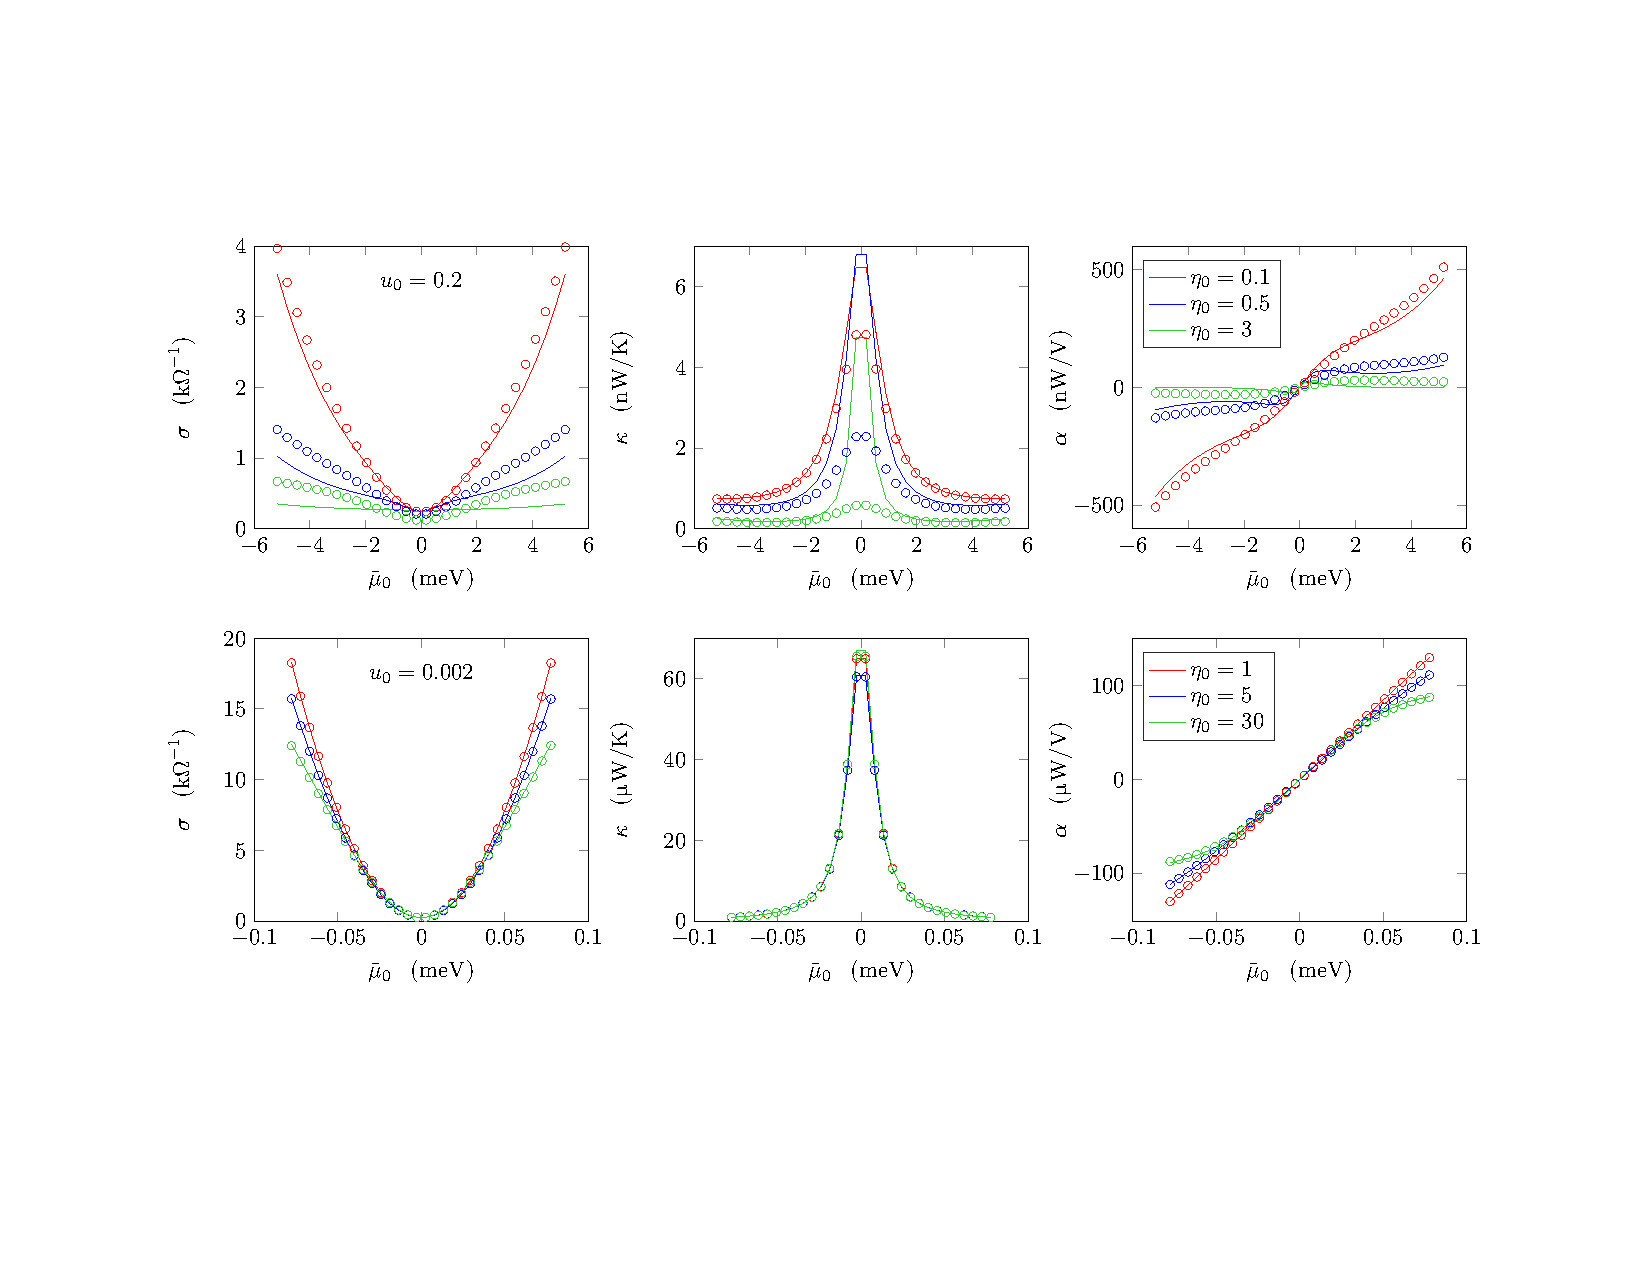
\includegraphics[width=6in]{viscosityplot.pdf}
\caption{Numerical computations of transport coefficients with $C_1=C_2=\sigma_0=1$ and $C_4=0$.   The top row has $u_0=0.2$, and the bottom row has $u_0=0.002$.   Solid lines are our theoretical results (using the particular disorder realizations studied) and the circular markers are numerical results.   Averages are taken over 20 disorder realizations.  $T_0=75$ K and we employ the value of $v_{\mathrm{F}}$ in graphene.  }
\label{viscfig}
\end{figure}

We also show the consequences of a non-zero $C_4$ in Figure \ref{c4fig}.   The most important effect of $C_4$ is that $n$ and $\bar\mu_0$ are no longer proportional -- in particular, when $C_4>0$ we see that at larger $n$ both $\sigma$ and $\alpha$ decrease much more slowly with $n$.   Whenever $C_4\ne 0$, the equations of state become badly behaved at large $\mu$,  because $s(\mu)$ or $n(\mu)$ becomes a non-monotonically increasing function.  At lower temperatures ($T\lesssim 50$ K) in Figure \ref{mainfigT}, this begins to be an issue in the codes for the equations of state  we use to compare to experiment.  This implies that higher order terms in the equations of state (associated with more fit parameters) are necessary.

\begin{figure}[t]
\centering
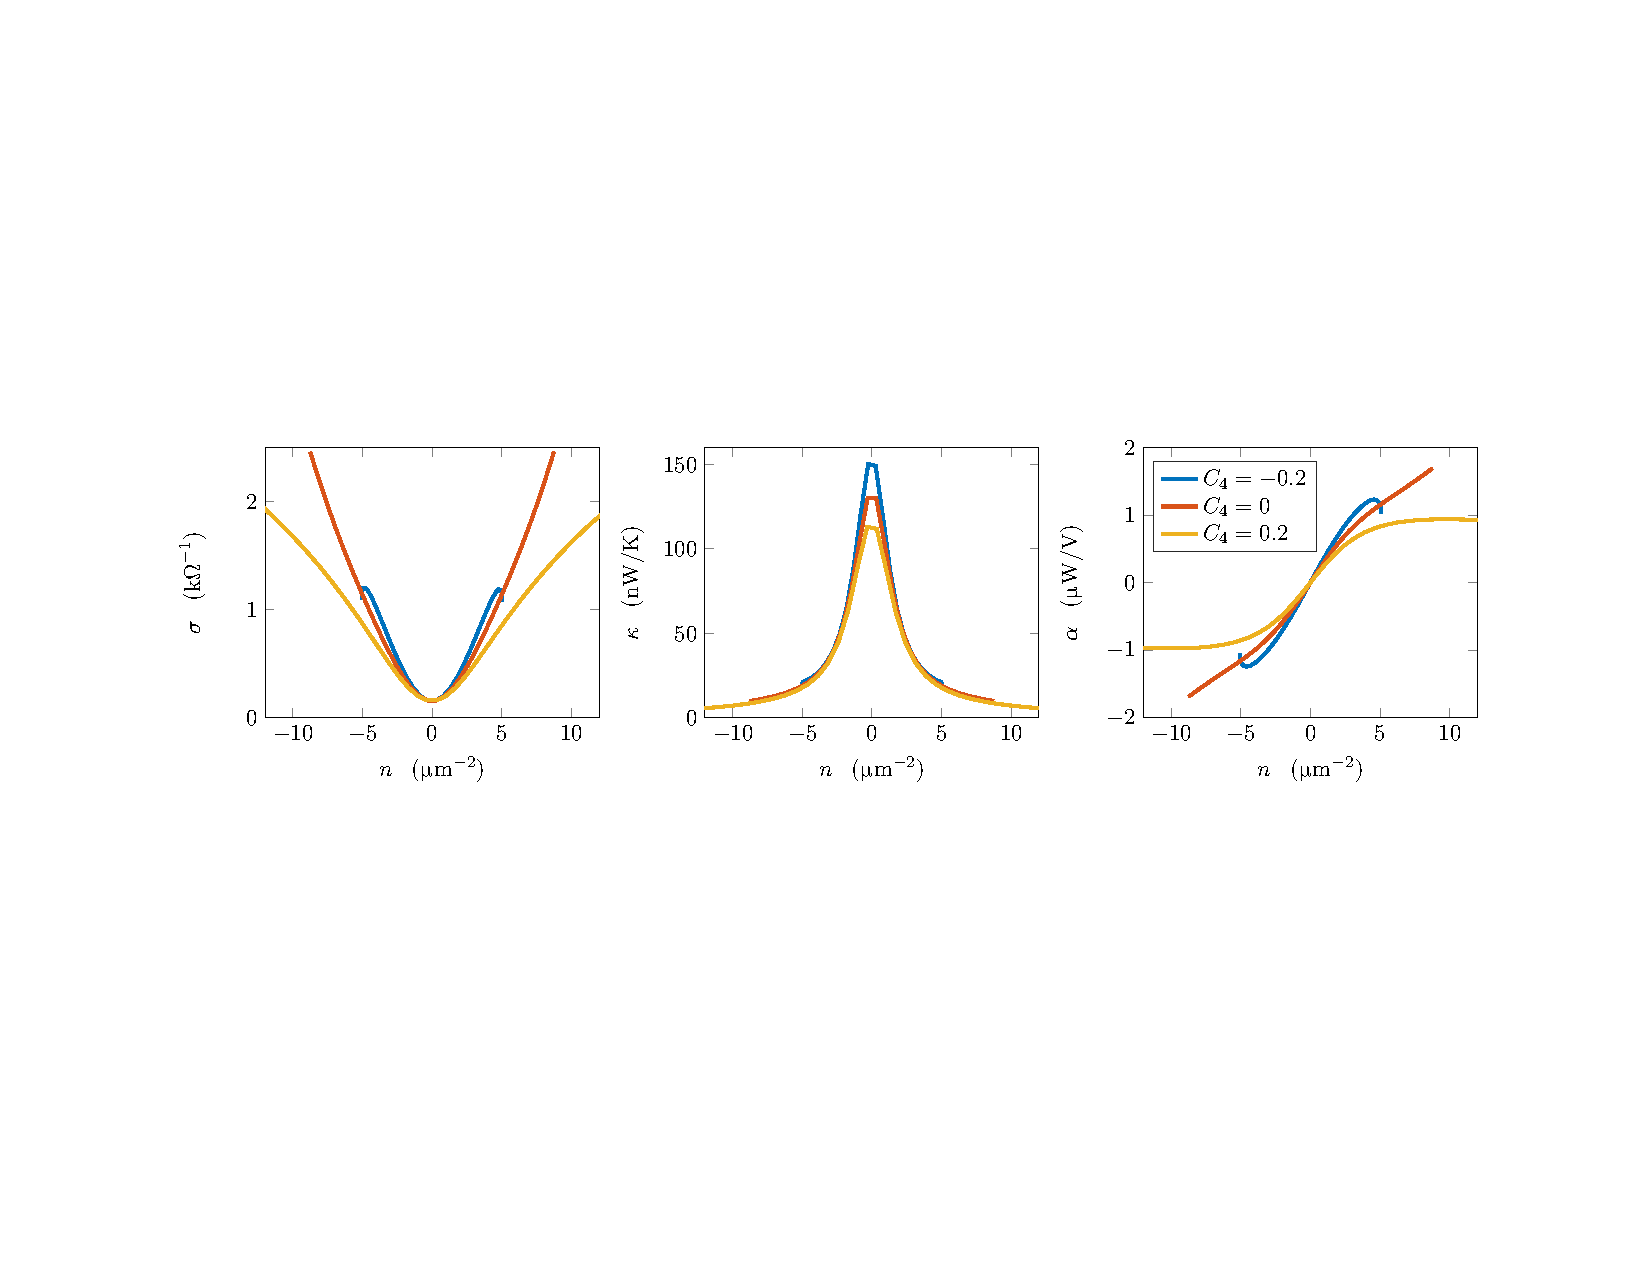
\includegraphics[width=6in]{c4plot.pdf}
\caption{Numerical computations of transport coefficients with varying $C_4$, $C_1=\sigma_0=1$, $\eta_0=3$, $C_2=0.2$ and $u_0=0.2$.    The sharp change in behavior when $C_4<0$ is a consequence of $n(\mu)$ not being monotonically increasing at large $\mu$.    Averages are taken over 20 disorder realizations.  $T_0=75$ K and we employ the value of $v_{\mathrm{F}}$ in graphene.  }
\label{c4fig}
\end{figure}


\subsection{Comparison to Experiment}
%A non-trivial check on our theory is to study $\kappa$ and $\sigma$ as a function of $T$.   \cite{crossno} also reported many measurements of these transport coefficients at the Dirac point,  and Figure \ref{mainfigT} compares of our numerical simulations to experimental data.   We have not averaged over disorder and finite size effects or shown its size,  as finite size disorder is not uncorrelated pointwise, and its dominant effect seems to be only to globally rescale $\sigma$ and $\kappa$.    Our theory must break down at $T<40$ K,\footnote{Indeed,  disorder is so large at $T\lesssim 50$ K that in our simulations there are a few locations where $s<0$, implying that higher orders in the thermodynamic equations of state must be included.   Although physically nonsensible, $s<0$ does not make our differential equations unstable or ill-posed, and so we have shown these data points for completeness.}  where the low temperature and large charge puddles ($u \sim k_{\mathrm{B}}T$) restore the Wiedemann-Franz law,  and at high temperatures $T>80$ K, where electron-phonon couplings no longer appear negligible.    The satisfactory fit of our theory to experiments gives us confidence that our hydrodynamic theory is correctly capturing the dominant transport near the Dirac point.  
%
% $\kappa\sim T^5$ is a reasonable fit to both the experimental and numerical curves in Figure \ref{mainfigT}, albeit this scaling only holds for $40<T<70$ experimentally.   This can be understood analytically as follows:  when $n=0$, the dominant scaling of $\tau$ comes from the first term in (\ref{taumain}), and so we find  $\tau \sim \epsilon+P \sim T^3$ and $s\sim T^2$,  which directly implies $\kappa \sim T^5$.   The small growth in $\sigma(T)$ at $n=0$ cannot be captured by arguments at leading order in perturbation theory.   
%
%In obtaining this fit we have assumed that the correlation length $\xi = l_{\mathrm{ee}}$ at all temperatures.    While the fit to $\kappa(n)$ is not sensitive to keeping $\xi$ fixed instead,   the fit to $\sigma(n)$ becomes notably worse, with $\sigma(T)$ a much more rapidly decreasing function.   We do not have a microscopic understanding of how the local chemical potential should change as a function of temperature in the hydrodynamic regime, and this is an important question for future work.   We do assume that $u$ is $T$-independent.

We now describe in more details the lessons to be drawn from our fit to experimental data, shown in Figures \ref{mainfig} and \ref{mainfigT}.   Due to a total of 6 fit parameters (3 which determine the overall scales in the plots, and 3 which alter the shapes of curves),  we did not perform an exhaustive analysis and find a statistically optimal fit.   We found that most choices of parameters do not agree well with data, and the fit we have presented serves as a proof of principle that hydrodynamics can explain many important features of the experiment \cite{Crossno1058}, as we now discuss.

%One practical issue in our hydrodynamic approach in the strongly interacting regime is the lack of robust theoretical predictions for the thermodynamic and hydrodynamic coefficients.   This leads to a large number of fitting parameters when comparing to data.   It is of great importance to find robust features of all simulations that are insensitive to all fit parameters.  

 To obtain data at lower temperatures, we have taken disorder realizations from $T_0=75$ K, using our standard assumption $\xi=l_{\mathrm{ee}}(T_0=75\; \mathrm{K})$, and simply lowered the temperature.  We also keep $u_0T_0$ constant as a function of $T_0$.  Formally, this implies that at lower temperatures $\xi<l_{\mathrm{ee}}$, as $l_{\mathrm{ee}}\sim T^{-1}$;  this may be problematic for the validity of hydrodynamics.    A conservative solution, employing the rescaling symmetries of our theory, is to simply double $\xi$,  and quadruple $\eta_0$:  all data is exactly identical, except that for all data points taken in Figure \ref{mainfigT},  $\xi>l_{\mathrm{ee}}$ and $\eta_0$ increases.

Figure \ref{Tscalefig} revisits the $T$-dependence in $\kappa$.  Assuming that disorder is weak, we employ (\ref{drudeeq}) and (\ref{taumain}) to determine the scaling of $\kappa$:  since  $s\sim T^2$, $\epsilon+P\sim T^3$, $\partial n/\partial \mu \sim T$, and the viscosity dependence in $\tau$ is negligible, we obtain $\tau \sim T$ and $\kappa \sim T^3$.   That numerics and experiment are not consistent with this power law is a sign of the strong non-perturbative effects, and suggests that observing  power law signatures of hydrodynamics may only be possible in the cleanest samples:
%This scaling can be derived analytically from (\ref{drudeeq}) and (\ref{taumain}): $s\sim T^2$, $\epsilon+P\sim T^3$, and the viscosity dependence in $\tau$ is negligible, leading to $\tau \sim T^3$.   Combining these results together we obtain $\kappa \sim T^5$.   This scaling law is a very robust prediction of our hydrodynamic approach and serves as a crucial test of its validity, working under the assumption that $\mu_0$ is $T$-independent.
% Although we do not have a large range of data in which we see the Dirac fluid, the fit of $\kappa(n=0,T)\sim T^5$ in the Dirac fluid is more consistent with the  experimental data
see Figure \ref{Tscalefig}.    Figure \ref{Tscaletheoryfig} suggests that the sharp dependence in $T$ observed in experiment is a consequence of $C_4>0$ and is not a robust scaling regime.\footnote{For this particular simulation, the disorder becomes large enough at $T\lesssim 7.5$ K that disorder realizations with $C_4=0.1$ sometimes have unphysical thermodynamic behavior.}  As noted in \cite{Crossno1058}, this dramatic $T$-dependence of $\kappa$, in contrast with the very weak $T$-dependence of $\sigma$, at the Dirac point, is a tell-tale sign of hydrodynamics that is not captured by competing theories, such as the bipolar diffusion effect.
 


\begin{figure}[t]
\centering
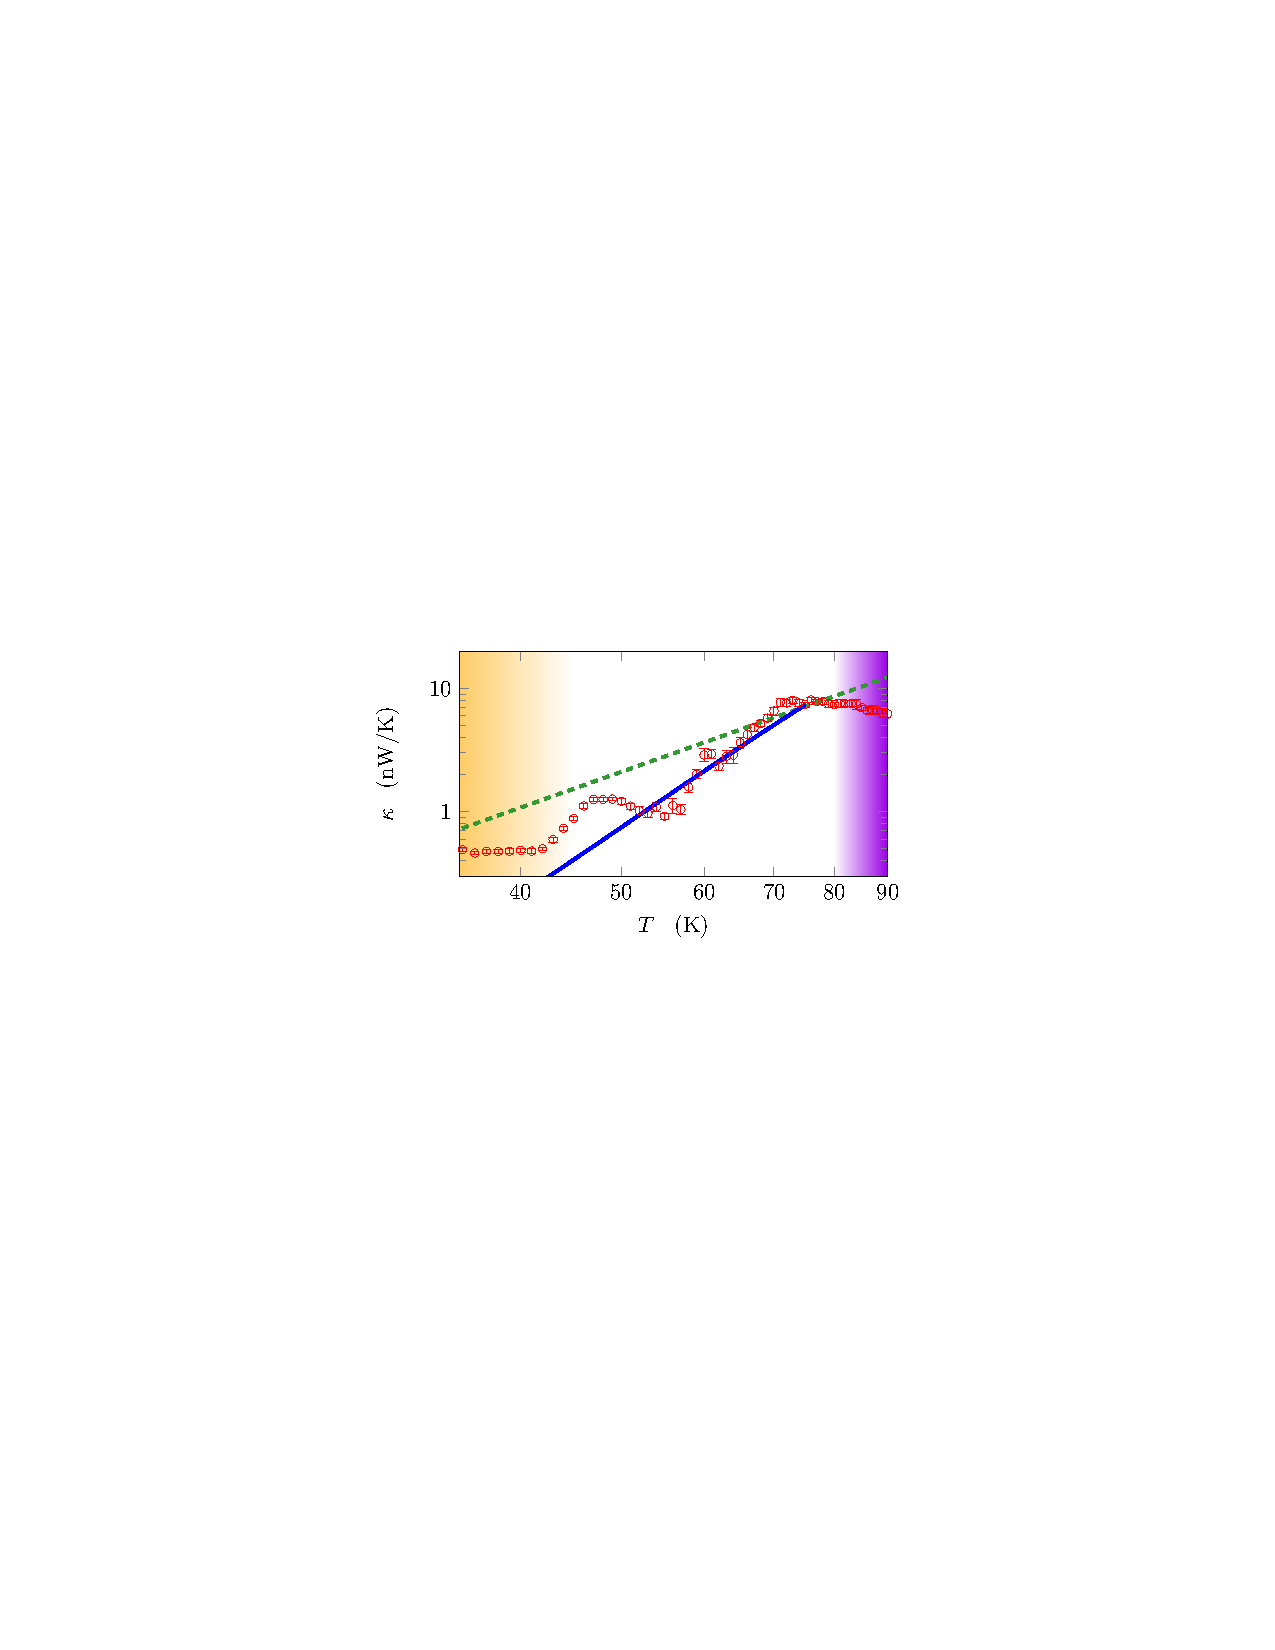
\includegraphics[width=3.5in]{Tscaleplot.pdf}
\caption{A comparison of our numerical computation of $\kappa(T)$ with experimental results of \cite{Crossno1058}  at the charge neutrality point ($n=0$).   The red data points are experimental data from \cite{Crossno1058}, the blue curve is our disorder-averaged simulation (using identical parameters to Figure \ref{mainfigT}), and the green dashed curve is the perturbative prediction $\kappa \sim T^3$ for comparison.  Data is shown on a log-log scale.  The yellow shaded region denotes where Fermi liquid behavior is observed; the purple shaded region denotes the likely onset of electron-phonon coupling.   }
\label{Tscalefig}
\end{figure}

\begin{figure}[t]
\centering
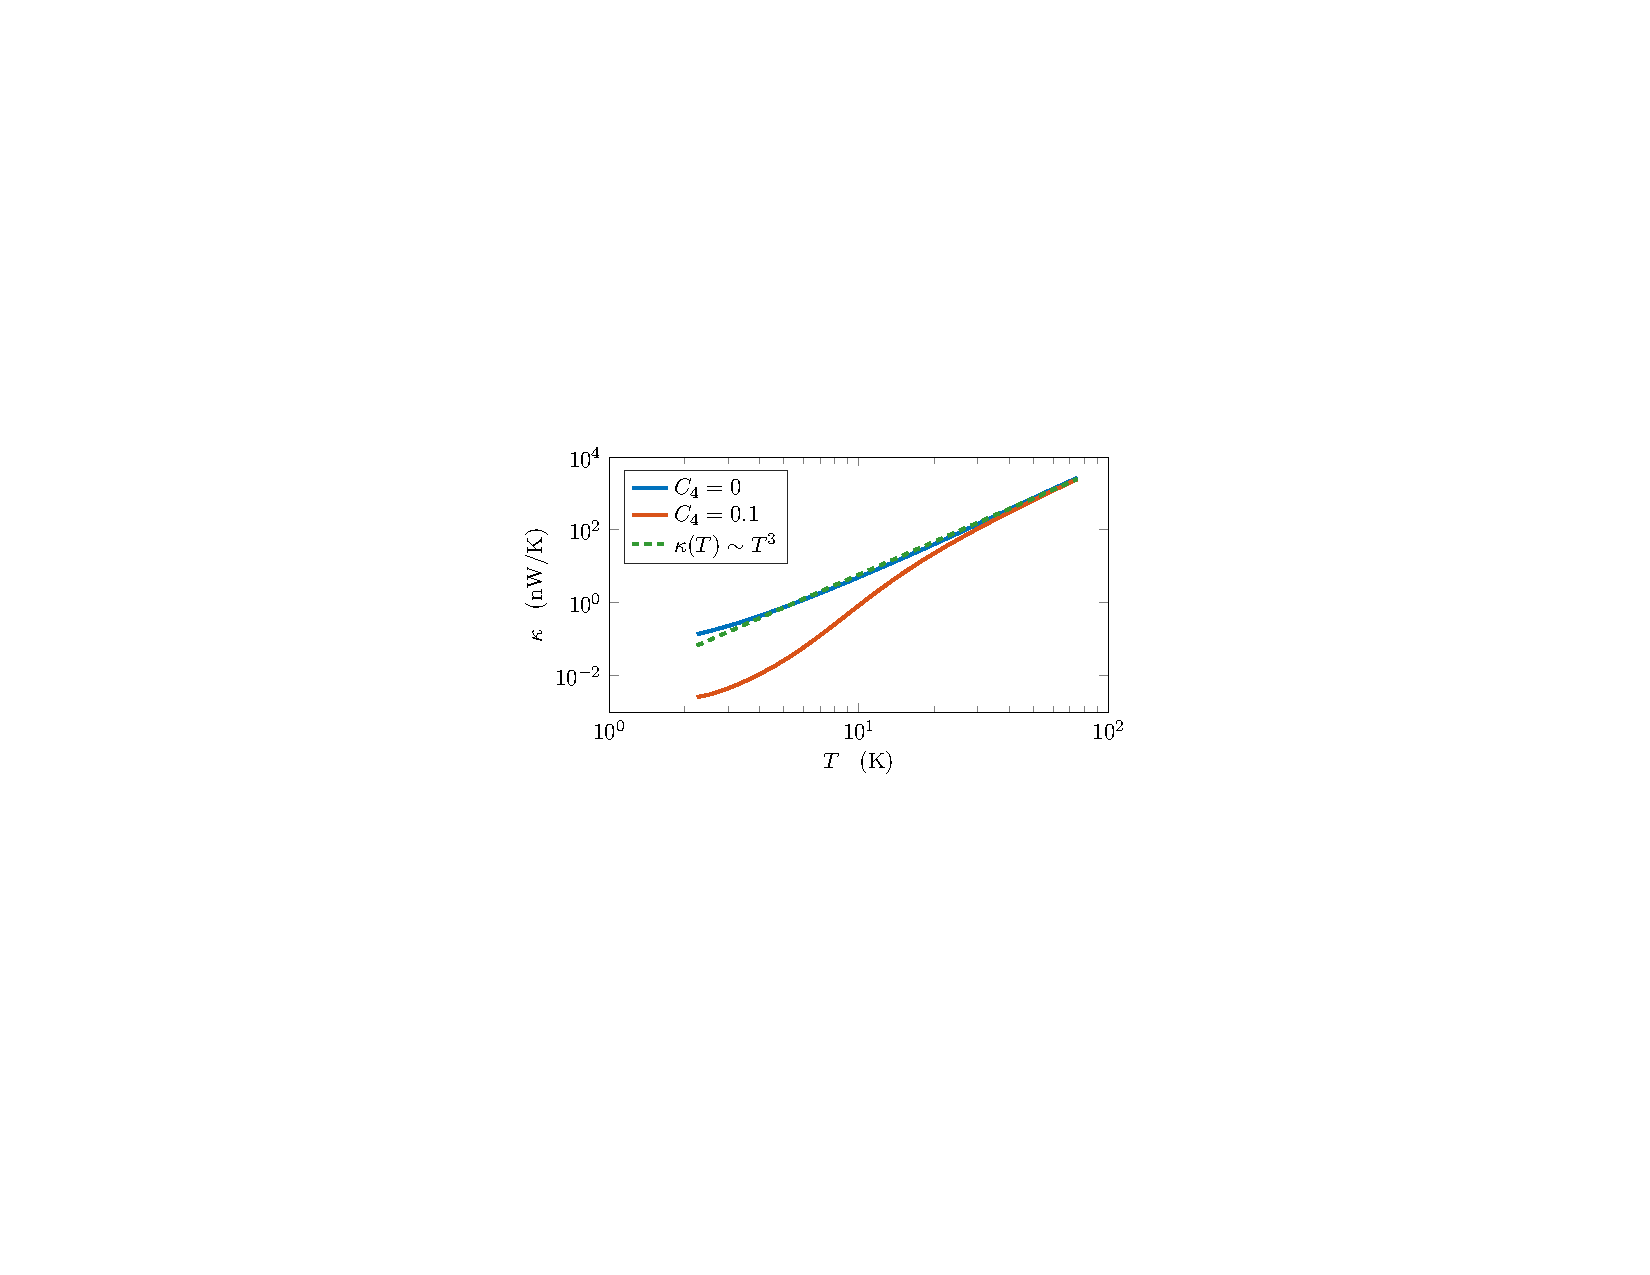
\includegraphics[width=3.5in]{kappaTC4plot.pdf}
\caption{A comparison of $\kappa(T)$ in simulations with varying $C_4$.  We take $C_0=1$, $C_2=\eta_0=0.1$, $\sigma_0=1$, $u_0=0.1$ (at $T_0=75$ K).   At large $T$ both scenarios have $\kappa \sim T^3$;  at lower $T$ the fluid with $C_4>0$ undergoes a dramatic drop in $\kappa(T)$, similar to that observed in experiment.}
\label{Tscaletheoryfig}
\end{figure}

The fits to $\sigma(n)$ and $\sigma(T)$ are not as good as the fits to $\kappa$.  Nonetheless, our theory does help to explain the slow growth in $\sigma$ away from the Dirac point, as a consequence of a fluid with both non-negligible viscosity and large disorder, as in Figure \ref{viscfig}.   Our simulations also correctly predict that the conductivity is an increasing function of $T$,  an entirely non-perturbative effect, in Figure \ref{mainfigT}.   This is at odds with predictions from kinetic theory in the Dirac fluid, which predict that $\sigma(n=0,T) \sim \alpha^{-2}_{\mathrm{eff}}$ should be decreasing with $T$ due to the $T$-dependence in $\alpha_{\mathrm{eff}}$ \cite{muller2}.   Any residual contact resistance \cite{wang13} will also increase the growth rate of $\sigma(n)$ away from the Dirac point, and as such will be closer fit by our numerical results in Figure \ref{mainfig}.


The most surprising thing about the fit is the  large values of all coefficients, compared to previous theories.   For example, it is predicted \cite{vafek, schmalian} that $C_0 \lesssim 3.4$, and we find $C_0 \sim 10$.   This is a direct consequence of the large values of the density $n$ over which the Dirac fluid is present (as measured by where strong deviations from the Wiedemann-Franz law occur).  The naive theoretical estimate is that the Dirac fluid should not extend past about $n\sim 40 \; \mmu \mathrm{m}^{-2}$,\footnote{We have used theoretically predicted values of $C_0$ and $C_2$ \cite{schmalian}, and assumed that the Dirac fluid ends when the $\mu$-dependent contribution to $s$ is comparable to the $T$-dependent contribution.} yet we see the Dirac fluid all the way to about $n\sim 200 \; \mmu\mathrm{m}^{-2}$; we will comment more on this issue shortly.    As in non-relativistic fluid dynamics, our hydrodynamic theory has a large number of rescaling symmetries (Appendix \ref{apprescale}), and these rescaling symmetries turn out to lead to very large values for all hydrodynamic coefficients as a consequence of the large scale on the density axis in Figure \ref{mainfig}.

Another consequence of this rescaling is a dramatically large shear viscosity:  $\eta_0\sim 100$.   It is now canonical to normalize this by the entropy density, and so the ``proper units" to measure $\eta$ in are $\eta_0/C_0\approx 10$.   This scaling is a consequence of a proposition \cite{Kovtun:2004de} that strongly coupled theories would have $\eta/s \approx \hbar/4\mpi k_{\mathrm{B}}$, or $\eta_0/C_0 \approx 1/4\mpi$.  The viscosity is a helpful measure of the interaction strength in a theory;  if the interactions are perturbatively controlled by a small parameter $g$, then we expect $\eta \sim g^{-2}$;  only when the interaction strength is large can $\eta \sim s$, up to a prefactor of order unity.  Hence, coming close to saturating the bound of \cite{Kovtun:2004de} is a signature that the fluid is strongly interacting. Our estimate for $\eta_0/C_0$ is about 100 times larger than the bound of \cite{Kovtun:2004de}.   Smaller values of $\eta/s \sim 0.5 \hbar /k_{\mathrm{B}}$ have been reported in other experiments in cold atomic gases \cite{cao} and quark-gluon plasma \cite{luzum}.   The possibility of adding the Dirac fluid to a list of strongly interacting quantum fluids is tantalizing, and a more direct measure of $\eta$ in the Dirac fluid is of interest. 

One possibility is that our bare coefficients $C_0$, $\eta_0$ etc. are anomalously large because \cite{Crossno1058} has measured the average charge density in the entire sample.   However, some regions of the sample (notably close to the contacts on the edges \cite{huard}, or regions very close to impurities) may have such large local values of $\mu_0$ that they are always in a Fermi liquid regime.  So long as these Fermi liquid regimes do not percolate across the entire sample, our hydrodynamic description of transport may be quite reasonable in the bulk.  However, these regions have a much smaller compressibility, and so can absorb a lot of charge relative to a clean Dirac fluid.    It may be that the total averaged charge density is then not equal to the averaged hydrodynamic charge density,  leading us to overestimate $n$.   Rescaling $n \rightarrow \lambda n$ would rescale $C_0 \rightarrow \lambda C_0$ and $\eta_0 \rightarrow \lambda^2 \eta_0$.   Choosing $\lambda = 0.2$, in accordance with our previous estimates on the regime of the Dirac fluid at $T_0\sim 75$ K, we obtain $C_0\sim 2$ and $\eta_0/C_0 \sim 2$, which are both reasonable for a strongly interacting fluid.   

As noted previously, we expect that future measurements in cleaner samples may give a wider separation between $l_{\mathrm{ee}}$ and $\xi$.   Together with a better understanding of edge effects and the charge puddle profile, we expect this approach to lead to cleaner estimates of $C_{0,2,4}$, $\eta_0$ and $\sigma_0$. 

\section{Phonons in Graphene}\label{secphonon}
Throughout this work we have neglected the effects of electron-phonon coupling in graphene \cite{fong, fong2}.   In this section, we provide some brief qualitative comments on the role of electron-phonon coupling in the experiment \cite{Crossno1058}, and discuss signatures for future experiments.

Generically, phonons extract both energy and momentum from the electronic fluid, and in doing so hamper a hydrodynamic description.\footnote{The hydrodynamic description of transport reduces to a diffusion equation for the conserved electrical current.   Historically, this was modeled via resistor networks \cite{kirkpatrick, derrida}.}  In graphene, the acoustic branch(es) of phonons have dispersion relation \cite{hwang07} \begin{equation}
\omega_{\mathrm{ac}}(\mathbf{q}) \approx \hbar v_{\mathrm{a}} |\mathbf{q}|
\end{equation} with  $v_{\mathrm{a}}\approx 2\times 10^4 $ m/s and so $v_{\mathrm{a}} \ll v_{\mathrm{F}}$.   By considering conservation of energy and momentum in electron-phonon scattering events, one finds that the phonon energies are negligible, and thus the scattering event can be treated as elastic from the point of view of the electrons.

If only acoustic phonons couple to the electronic fluid, we may approximate that the momentum conservation equation is modified, following the phenomenology of \cite{hkms}: \begin{equation}
\partial_\mu T^{\mu i} \approx F^{\nu i}_{\mathrm{ext}} J_\nu - \frac{T^{ti}}{\tau_{\mathrm{a}}} .
\end{equation}
The latter term implies that the momentum of the electronic fluid degrades at a constant rate $\tau^{-1}_{\mathrm{a}}$, which we take to be \begin{equation}
\frac{1}{\tau_{\mathrm{a}}} = \mathcal{B} T^a,
\end{equation}where $a>0$ and $\mathcal{B}>0$ are constants that are phenomenological.  \cite{hwang07} computed their values using kinetic theory and found $a=4$ far from the Dirac point.   This effect has been observed experimentally \cite{efetov},  but $a$ is expected to change near the Dirac point.   Following arguments similar to \cite{ashcroft, hwang07}, we can estimate $a$ by assuming a quasiparticle description of transport, and that the dominant events are absorption or emission of a single phonon.   Since acoustic phonons cannot effectively carry away energy, a Dirac quasiparticle of energy $\epsilon$ can scatter into $\sim \epsilon$ states.   All phonons with relevant momenta are thermally populated, and we estimate the scattering rate to be proportional to the momentum of the phonon.   Thus we estimate, using that the typical quasiparticle energy is $\epsilon \sim T$, $a=1+1=2$.\footnote{As there is no large Fermi surface with $\mu \gg k_{\mathrm{B}}T$, no further corrections to $a$ are necessary, as in usual metals.}

Assuming that the charge puddles are small and can be accounted for perturbatively,  $\kappa$ is approximately given by (\ref{hkmseq}) at the Dirac point, with \begin{equation}
\frac{1}{\tau} \approx  \frac{u^2}{2\sigma_{\textsc{q}} (\epsilon+P)}\left(\frac{\partial n}{\partial \mu}\right)^2 +  \mathcal{B}T^a = \frac{\mathcal{A} u^2}{T^b} + \mathcal{B}T^a.
\end{equation}
Our analytic theory predicts $b=1$.  The contribution $\kappa$ from electron-phonon coupling is negligible so long as \begin{equation}
T \ll  T^* \equiv  \left(\frac{\mathcal{A}}{\mathcal{B}}u^2\right)^{\frac{1}{b+a}}.
\end{equation}
Note that $T^*(u)$ is an increasing function -- the weaker the disorder, the lower the temperature at which electron-phonon coupling cannot be neglected in the Dirac fluid.   The thermal conductivity scales as \begin{equation}
\kappa \sim \left\lbrace\begin{array}{ll}  T^{2+b} &\  T\ll T^* \\ T^{2-a} &\ T\gg T^*\end{array}\right.
\end{equation}
If $a>2$, we find phenomenology quite similar to that observed in \cite{Crossno1058}, with $\kappa(T)$ growing non-monotonically.   We also find that \begin{equation}
\kappa(T^*) = \mathcal{C} (T^*)^{2-a},
\end{equation}
a result which can be tested in experiment by measuring $T^*$ via the peak in $\kappa$ for different samples.  The prefactor of this proportionality $\mathcal{C}$ may not be very sensitive to the particular sample, since it is independent of $u$.   Figure \ref{ephfig} shows a sketch of $\kappa(T)$, accounting for acoustic phonons, in three samples with different disorder strengths $u$.   This mechanism is also consistent with the fact that the cleaner samples in \cite{Crossno1058} had peaks in $\kappa(T)$ at lower temperatures, which suggests our proposed mechanism for the non-monotonicity in $\kappa(T)$ is sensible.   Although our perturbative quasiparticle-based argument found $a=2$ above, the presence of local charge puddles may increase the effective value of $a$ to somewhere between 2 and 4, and lead to $\kappa(T^*)$ be a decreasing function.   A careful analysis of electron-phonon coupling in disordered Dirac fluids is worth more study.   

\begin{figure}[t]
\centering
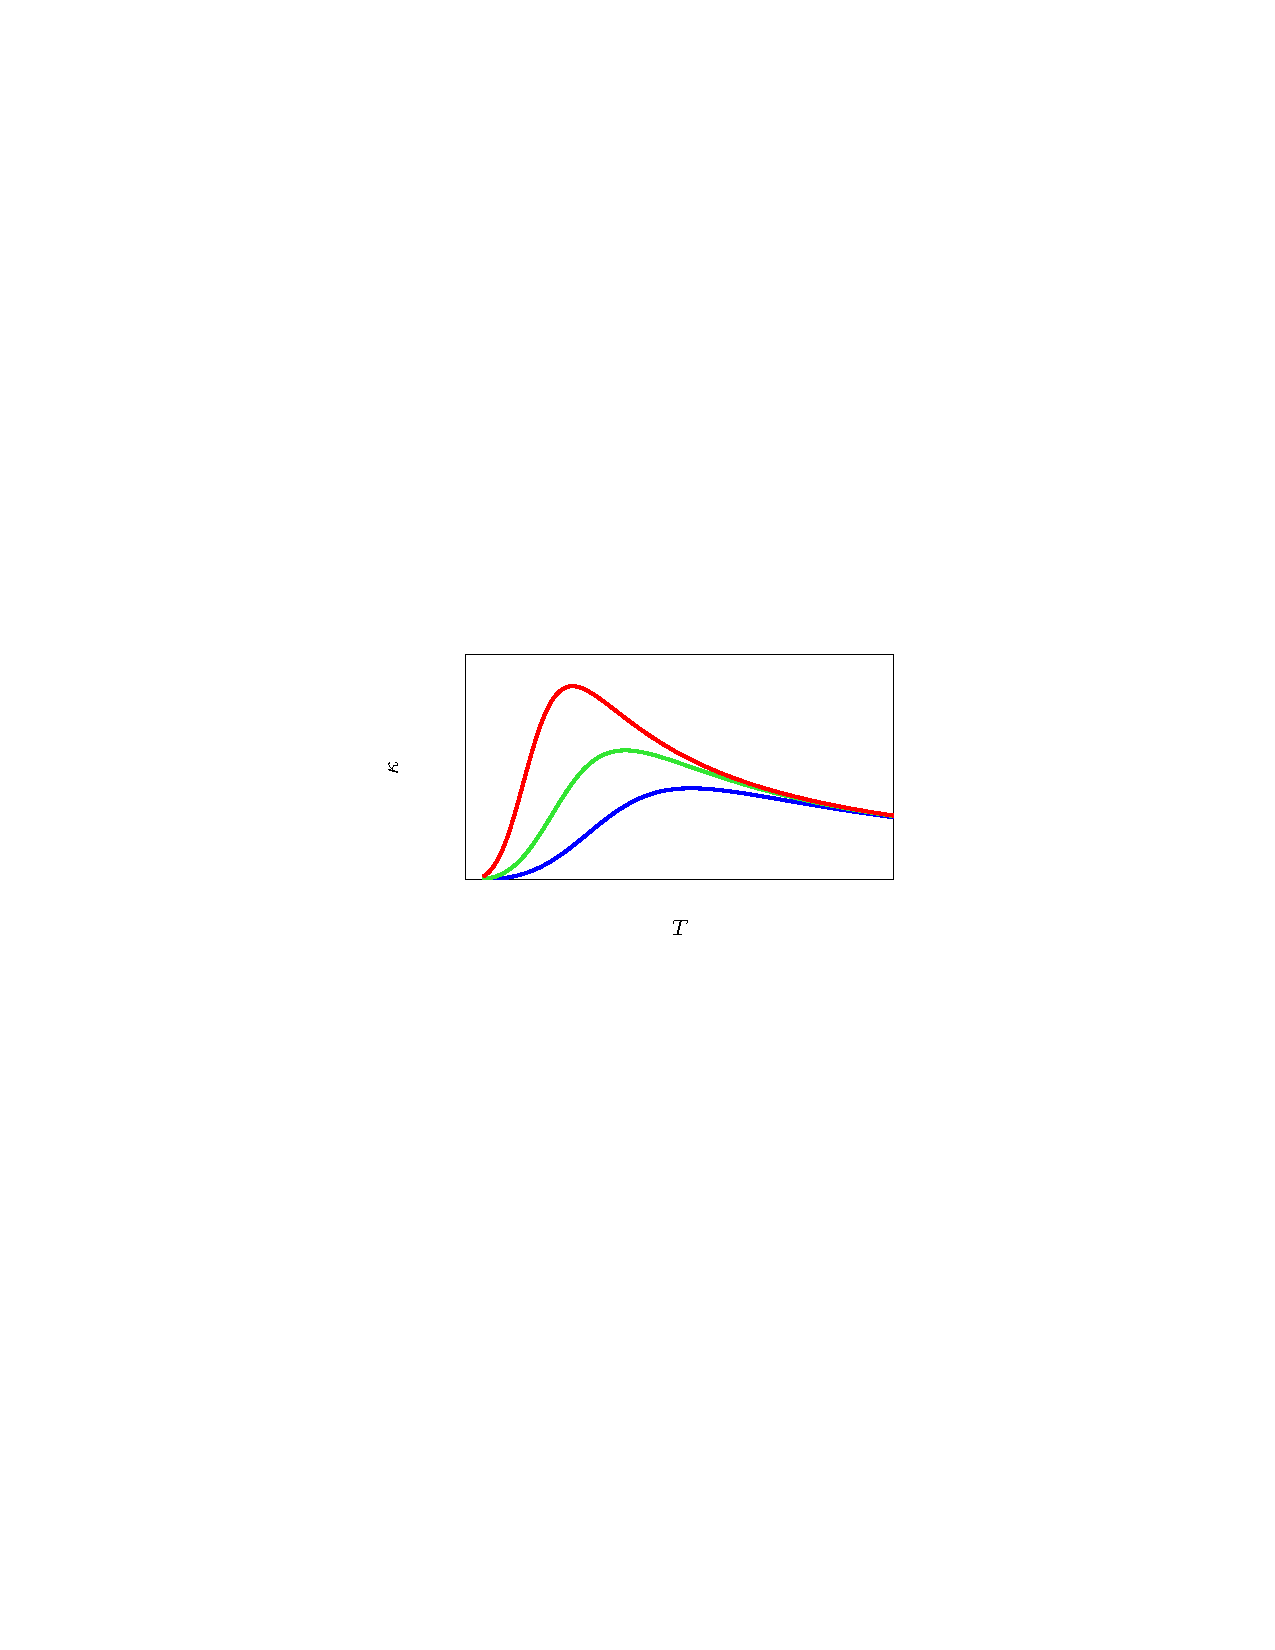
\includegraphics[width=3.5in]{ephsketchplot.pdf}
\caption{A sketch of $\kappa(T)$, accounting for coupling to acoustic phonons, for samples of graphene with three different amounts of disorder (measured by $u$).  We take $a=3$, $b=1$ in this plot.}
\label{ephfig}
\end{figure}


At higher temperatures, we expect optical phonons to couple non-negligibly to the electron fluid.   These phonons can exchange both energy and momentum effectively,  and at this point we expect the measured thermal conductivity to increase due to electron-phonon coupling.   In \cite{Crossno1058},  there is a sharp upturn in $\kappa(T)$ at all densities at temperatures of 100 K, which is likely due to activation of optical phonons in the boron nitride subtrate \cite{crossno2}.


\section{Conclusions}

We have developed a theory of transport in realistic hydrodynamic electron fluids near a quantum critical point.    This theory provides a substantially improved quantitative fit to $\kappa(n)$ and $\sigma(n)$ \emph{simultaneously}.    We have further found reasonable quantitative fits to $\sigma(T)$ and $\kappa(T)$ at the Dirac point, giving us valuable information about the mechanism of momentum relaxation beyond the theory of \cite{hkms}.

  Although we have managed to find fluids where the growth in $\sigma(n)$ is quite slow, there are still differences between the shape of $\sigma(n)$ found numerically and in experiment.   There are numerous possibilities for residual discrepancies.   One of the most important possibilities is that the disorder is so strong that the full thermodynamic equation of state is necessary -- in this paper, we have only kept the three leading order terms.   Alternatively, we may simply not have found the correct equation of state of graphene.  A disorder profile more subtle than superimposed sines and cosines may also be responsible for deviations with our theory, although our investigation into this possibility suggests that other disorder profiles cause $\sigma(n)$ to have more substantial density dependence.    We have assumed that the disorder profile is unaltered both by changes in $T$ and in $\bar\mu_0$.   This is a very strong assumption and need not be true.   Finally, there may be other sources of momentum relaxation, such as out-of-plane distortions in the graphene lattice, or interactions with phonons.   An understanding of the aforementioned issues is an important future task, though may be quite challenging given the possibility that strong interactions in the Dirac fluid at $T\sim 70$ K may lead to the failure of standard perturbative techniques.   The most fruitful direction for resolving at least some of these questions may be directly in experiments: for example, techniques to directly resolve the local charge density on length scales $\lesssim$ 10 nm are well known \cite{xue}, and can shed light into the evolution of $\mu_0$ as a function of $T$, as well as the spatial correlations in $\mu_0$.
  
Experimentally, it may be possible to generate samples of graphene with much weaker charge puddles using suspended devices \cite{bolotin, mayorov}.  Thermodynamic measurements can also be used to determine the coefficients $C_{0,2,4}$, though these measurements are complicated by the presence of disorder, as we discuss in Appendix \ref{appthermo}.   Nonetheless, measurements of the specific heat and compressibility in the Dirac fluid will serve as valuable guideposts for future hydrodynamic models.   Such measurements have been made in the Fermi liquid \cite{yacoby2007}, and their extension to the Dirac fluid form the basis for worthwhile experiments.

Previous experiments which measured the ac conductivity \cite{horng} were not in the hydrodynamic limit.   Comparing the momentum relaxation time $\tau$ between measurements of $\kappa$, and a putative Drude peak in ac transport, may provide a quantitative test of our theory.   Studying magnetotransport \cite{hkms} may also be a fruitful direction in experiments.  A theoretical discussion of transport at finite frequency and magnetic field beyond the weak disorder limit will appear elsewhere.   The thermopower  of graphene has recently been measured at $T\sim 200$ K \cite{ghahari},  and it would be interesting to measure $\sigma$, $\alpha$ and $\kappa$ in the same sample in the Dirac fluid and compare with our hydrodynamic formalism.


\begin{appendix}
\chapter{Appendix for Chapter 5} \label{appb}
Here we discuss the matrix element $M_{P_x\partial_x n}$, when the operator $\mathcal{O}$ which couples to the translational symmetry breaking field is not charge conjugation symmetric.   From the definition of the memory matrix, \begin{equation}
M_{P_x\partial_x n} = \frac{1}{\pi\mathrm{i}}\int \mathrm{d}\omega \int \mathrm{d}^d\mathbf{q} \; h(\mathbf{q}) \frac{\mathrm{Im}\left(-\mathrm{i}\omega G^{\mathrm{R}}_{\mathcal{O}\partial_x n}(\mathbf{q},k_x,\omega)\right)}{\omega(\omega - z)},
\end{equation}where we have related $\dot{P}_x$ to $\mathcal{O}$.   Let us discuss the general structure of this Green's function.   In fact, noting that $z$ is just above the real axis, we find that \begin{equation}
M_{P_x\partial_x n} = \int \mathrm{d}^d\mathbf{q} \; h(\mathbf{q}) \mathrm{Re}\left(G^{\mathrm{R}}_{\mathcal{O}\partial_xn}(\mathbf{q},k_x,0)\right).
\end{equation} We know that $G^{\mathrm{R}}_{\mathcal{O}\partial_x n} \sim h$, as this Green's function does not obey translation invariance, and thus must be proportional to $h$.   Furthermore, so long as charge is an exactly conserved quantity, and this Green's function is analytic in a neighborhood of $k_x=0$, we conclude that $G^{\mathrm{R}}_{\mathcal{O}\partial_x n} \sim hk_x$.    Thus we conclude that $M_{P_x\partial_x n} \sim h^2k_x$.

Next, let us consider the corrections to the conductivity.   For simplicity, we focus on the case where $B=0$, but similar considerations will hold in the more general case. The full memory matrix $\mathfrak{m}$ is block diagonal, and, considering only $xx$ indices, is \begin{equation}
\mathfrak{m} = \left(\begin{array}{cc} h^2 \mathcal{B}  &\   h^2k_x \mathcal{A} \\ h^2 k_x \mathcal{A} &\  \sigma_{\textsc{q}}k_x^2 \end{array}\right)
\end{equation}
with $\mathcal{A}$ and $\mathcal{B}$ chosen as functions which are not perturbatively small.    We find \begin{equation}
\mathfrak{m}^{-1} = \frac{1}{h^2k_x^2\mathcal{B}\sigma_{\textsc{q}}-k_x^2h^4\mathcal{A}^2} \left(\begin{array}{cc} \sigma_{\textsc{q}}k_x^2 &\   -h^2k_x \mathcal{A} \\ -h^2 k_x \mathcal{A} &\ h^2 \mathcal{B}  \end{array}\right) \approx \left(\begin{array}{cc} 1/h^2\mathcal{B} &\   - \mathcal{A}/\mathcal{B}\sigma_{\textsc{q}}k_x \\ - \mathcal{A}/\mathcal{B}\sigma_{\textsc{q}}k_x &\ 1/\sigma_{\textsc{q}}k_x^2  \end{array}\right)
\end{equation}The correction to the conductivity as given in (\ref{eqb0}) is \begin{equation}
\delta \sigma_{xx} = -\frac{2\mathcal{AQ}}{\mathcal{B}}.
\end{equation}
This is, in our limit, much smaller than either $\sigma_{\textsc{q}}$ or $\mathcal{Q}^2\tau/\mathcal{M}$.   Logically, we should think of this as much smaller than $\sigma_{\textsc{q}}$ since we argued previously that either $\sigma_{\textsc{q}}$ must be anomalously large, or $\mathcal{Q}$ must be very small, in order for $\sigma_{\textsc{q}} \sim \mathcal{Q}^2\tau/\mathcal{M}$ to be possible.   (If $\tau$ is anomalously large and $\sigma_{\textsc{q}}$ is negligible, then we should generically expect $\delta \sigma_{xx}$ to also be negligible).    Thus, it is consistent to ignore these corrections to the memory matrix at leading order.

\chapter{Appendix for Chapter 8}


\section{Sample Fabrication}
Single layer graphene is encapsulated in hexagonal boron nitride on an n-doped silicon wafer with 285 nm SiO$_2$ \cite{wang13} and is subsequently annealed in vacuum for 15 minutes at 350 $^\circ$C. It is then etched using reactive-ion-etching (RIE) to define the width of the device. A second etch mask is then lithographically defined to overlap with the sample edge, leaving the rest of the sample rectangular shaped with the desired aspect ratio. After the RIE is performed, the same etch mask is used as the metal deposition mask, upon which Cr/Pd/Au (1.5 nm / 5 nm / 200 nm) is deposited. The resulting Ohmic contacts show low contact resistances and small PN junction effects due to their minimum overlap with device edge. 

\subsection{Optimizing samples for high frequency thermal conductivity measurements}
To measure the electronic thermal conductivity $\kappa_{\mathrm{e}}$ of graphene using high frequency Johnson noise the sample design should be made with three additional considerations: stray chip capacitance, resistance of the lead wires, and sample dimensions that enhance electron diffusion cooling over phonon coupling. 

Johnson noise thermometry (JNT) relies on measuring the total noise power emitted in a specified frequency band and relating that to the electronic temperature on the device; to maximize the sensitivity, high frequency and wide bandwidth measurements should be made \cite{crossno2}. In the temperature range discussed here, the upper frequency limit for JNT is typically set by the amount of stray capacitance from the graphene, lead wires, and contact pads to the Si back gate. This is minimized by using short, narrow lead wires and small (50 $\mmu$m $\times$ 50 $\mmu$m) bonding pads resulting in an estimated 4 pF stray capacitance. 

The amount of Johnson noise emitted between any two terminals is proportional to the mean electronic temperature between them where each point in space is weighted by its local resistance. Therefore, to maximize the signal coming from the graphene, contact resistance should be kept at a minimum.  To compensate for the narrow lead wires, we deposit a thicker layer (200 nm) of gold resulting in an estimated lead resistance of 50 $\mathrm{\Omega}$.  This, combined with an estimated interfacial contact resistance of $<135$ $\mathrm{\Omega}\cdot\mmu \mathrm{m}$ results in a total measured contact resistance of $<80$ $\mathrm{\Omega}$.  The interfacial contact resistance may be density dependent and we estimate it to be $\lesssim 100$--$300\; \mathrm{\Omega}\cdot\mmu\mathrm{m}$.   The most important effect of this contact resistance is likely the thermal resistance associated to the contacts, which may limit the maximal observable Lorenz ratio.   As such, the true value of $\mathcal{L}$ is likely slightly higher than what we measure. 

Lastly, to effectively extract $\kappa_{\mathrm{e}}$ from the total electronic thermal conductance $G_{\mathrm{th}}$ we want to enhance the electron diffusion cooling pathway with respect to the electron-phonon cooling pathway (see below). This can be accomplished by keeping the length of the sample short as the total power coupled into the lattice scales as the area of the device while diffusion cooling scales as $1/R$. In addition, the device should be made wide to minimize the effects of disordered edges. We find these high aspect ratio samples ($\sim$ 3:1) are ideal for our measurements and serve the additional purpose of lowering the total sample resistance allowing us to impedance match over a wider bandwidth.

\begin{table}[t]

\centering

\begin{tabular}{| l | c | c | c |}\hline
&\  S1 &\ S2 &\ S3 \\\hline
length ($\mmu$m) &\ 3 &\ 3 &\ 4 \\
width ($\mmu$m) &\ 9 &\ 9 &\ 10.5 \\
mobility ($10^5\; \mathrm{cm}^2\cdot \mathrm{V}^{-1}\cdot \mathrm{s}^{-1}$) &\ $3$ &\ $2.5$ &\ $0.8$ \\
$n_{\mathrm{min}}$ ($10^9$ cm$^{-2}$) &\ 5 &\ 8 &\ 10 \\\hline
\end{tabular}
\caption{Basic properties of our three samples.}
\label{table1}
\end{table}

\section{Device Characterization}
In this study we measure three graphene devices encapsulated in hexagonal boron nitride (hBN), whose basic properties are detailed in Table \ref{table1}.    All devices are two-terminal with mobility estimated as \begin{equation}
\mu\approx \frac{L}{neRW},
\end{equation}
where $L$ and $W$ are the sample length and width respectively, $e$ is the electron charge, and $n$ is the charge carrier density.   The gate capacitance per unit area $C_{\mathrm{g}}\approx 0.11\; \mathrm{fF}/\mmu \mathrm{m}^2$ is estimated considering the 285 nm SiO$_2$ and $\sim 20$ nm hBN dielectrics.   From this we estimate the charge density \begin{equation}
n=\frac{C_{\mathrm{g}}(V_{\mathrm{g}}-V_{\mathrm{d}})}{e}
\end{equation} where $V_{\mathrm{d}}$ is the gate voltage corresponding to the charge neutrality point (CNP) estimated by the location of the maximum of the curve $R(V_{\mathrm{g}})$.   Fig. \ref{figs1} shows the resistance of all samples as a function of gate voltage.

 \begin{figure}[t]
 \centering
\includegraphics[width=3in]{SM_V2-01-eps-converted-to.pdf}
\caption{2-terminal resistance $R$ vs. back gate voltage for the 3 samples used in this report.}
\label{figs1}
\end{figure}

\section{Johnson Noise Thermometry}
The full Johnson noise thermometry (JNT) setup used in this study is outlined in detail in \cite{crossno2}.   Here, we only give a brief synopsis for completeness.

The electronic transport within a dissipative device can be determined by the high frequency noise power collected by a low noise amplifier as \begin{equation}
\left\langle V^2\right\rangle = k_{\mathrm{B}}T_{\mathrm{e}} \times \mathrm{Re}(Z)\Delta f \left[1-\left(\frac{Z-Z_0}{Z+Z_0}\right)^2\right]
\end{equation}where $Z$ is the complex impedance of the device under test, $Z_0$ is the impedance of the measure circuit (typically 50 $\Omega$) and $\Delta f$ is the bandwidth.   From this formula, we can see two critical components of JNT:  impedance matching over a wide bandwidth and low noise amplification.

Graphene devices have a typical channel resistance on the order of $h/4e^2 \sim 6\; \mathrm{k}\Omega$ near the CNP.   To compensate for this, we use an inductor-capacitor (LC) tank circuit mounted directly on the sample package to impedance match the graphene to the 50 $\Omega$ measurement network.  Fig.  \ref{figs2} shows the reflectance coefficient $\mathcal{R}=|S_{11}|^{2}$ for a typical graphene device after impedance matching.   The bandwidth and measurement frequency of our JNT is set by the Q-factor and LC time of this matchingnetwork.

 \begin{figure}
 \centering
\includegraphics[width=3in]{SM_V2-07-eps-converted-to.pdf}
\caption{Reflectance $\mathcal{R}=|S_{11}|^{2}$ for a graphene device impedance matched to 50 $\Omega$ near 125 MHz.}
\label{figs2}
\end{figure}

At 10 K, the power emitted by a resistor in a 1 Hz bandwidth is $\sim 10^{-22}$ W or $-190$ dBm.  To amplify this signal we use a SiGe low noise amplifier (Caltech CITLF3) with a room temperature noise figure of about 0.64 dB in our measurement bandwidth, corresponding to a noise temperature of about 46 K.   We operate the amplifier at room temperature, outside of the cryostat, to ensure it is unaffected by the 3--300 K temperature ramp used for thermal conduction measurements.  After amplification, a homodyne mixer and low pass filter define the measurement bandwidth and the power is found by an analog RF multiplier operating up to 2 GHz (Analog Devices ADL5931).  The result is a voltage proportional to the Johnson noise power which -- after calibration -- measures the electron temperature in the graphene device.

Calibration of our JNT device must be done on every sample as each device has a unique $R(T,V_{\mathrm{g}})$ and therefore couples differently to the amplifier.  The graphene device being measured is placed on a cold finger in a cryostat with varying temperature $T_{\mathrm{bath}}$.  With no excitation current in the graphene, we collect the JNT signal $V_{\mathrm{s}}(T,V_{\mathrm{g}})$ for all temperatures and gate voltage needed in the study, as shown in Fig. \ref{figs3}.   The linear temperature slope at each point gives a gain factor $g(T,V_{\mathrm{g}}) = \partial V_{\mathrm{s}}/\partial T$.

 \begin{figure}
 \centering
\includegraphics[width=3in]{SM_V2-06-eps-converted-to.pdf}
\caption{Output voltage $V_{\mathrm{s}}$ from the JNT measuring a graphene device with no excitation current.  This is used to calibrate the JNT to a given sample.}
\label{figs3}
\end{figure}


\section{Measuring electronic thermal conductance}

The procedure used to measure electronic thermal conductance is outlined in \cite{crossno2, fong, prober}.  A small sinusoidal current $I(\omega)$ is run through the graphene sample, causing a Joule heating power $P(2\omega)$ to be injected directly into the electronic system.  This causes a small temperature difference $\Delta T(2\omega) $ between the electronic temperature and the bath, described by Fourier's law: \begin{equation}
P = G_{\mathrm{th}} \Delta T.   \label{eqp1}
\end{equation}
Here $G_{\mathrm{th}}$ is the total thermal conductance between the electronic system and the bath.  The component of Johnson noise at frequency $2\omega$  is measured by a lock-in amplifier and then converted to a temperature difference $\Delta T$ using the gain $g(T,V_{\mathrm{g}})$ described in the previous section.  Fig. \ref{figs4} shows $T_{\mathrm{e}}$ as a function of heating current $I$ for a graphene device at three different bath temperatures:  3, 30 and 300 K.

 \begin{figure}
 \centering
\includegraphics[width=3in]{SM_V2-04-eps-converted-to.pdf}
\caption{The electronic temperature in an encapsulated graphene device as a function of heating current for three different bath temperatures.  $T_{\mathrm{e}}=T_{\mathrm{bath}}+I^2R/G_{\mathrm{th}}$.  The total thermal conductance between the electronic system and the bath is found through Fourier's Law (solid lines).}
\label{figs4}
\end{figure}

\section{Thermal model of graphene electrons}\label{s6sec}
In the regime presented here, $G_{\mathrm{th}}$ is dominated by two electronic cooling pathways.  Hot electrons can diffuse directly out to the contacts ($G_{\mathrm{diff}}$), or they can couple to phonons ($G_{\mathrm{el-ph}}$):  \begin{equation}
G \approx G_{\mathrm{diff}} + G_{\mathrm{el-ph}}.
\end{equation}
In a typical metal, electron diffusion is described by the WF law which is linear in $T_{\mathrm{e}}$. The electron-phonon cooling pathway has two components:  first, the electrons must transfer heat to the lattice via electron-phonon coupling, and then the lattice must conduct the heat to the bath. Fig. \ref{figs5} shows the simplified thermal diagram of the electronic cooling pathways in graphene, relevant to our experiment.

 \begin{figure}
 \centering
\includegraphics[width=1in]{SM_V2-10-eps-converted-to.pdf}
\caption{Simplified thermal diagram of the electronic cooling pathways in graphene relevant for our experimental conditions.  A current induces a heating power into the electronic system which conducts to the bath via two parallel pathways:  diffusion and coupling to phonons.}
\label{figs5}
\end{figure}

At low temperature, $G_{\mathrm{th}}$ is dominated by $G_{\mathrm{diff}}$, while at high temperature it is dominated by $G_{\mathrm{el-ph}}$. We plot in Fig. \ref{figsEPh} our data compared to two different experimental reports. For our device parameters, the heat transferred to the lattice by the supercollision mechansim is much smaller (green solid line) as verified by three independent experiments in Ref. \cite{Graham:2013vl, betz, laitinen}, based on the theories of Song-Reizer-Levitov \cite{Song:2012by} and Chen-Clerk \cite{Chen:2012et}. Similarly, the heat transferred to acoustic phonons is also smaller than the electronic diffusion term for our device geometry (purple solid curve) as verified by three sets of experiments in Ref. \cite{betz}, \cite{fong, fong2, crossno2, prober} based on the theories of Bistritzer-MacDonald \cite{Bistritzer:2009ht}, Tse-DasSarma \cite{Tse:2009il}, Viljas-Heikkalla \cite{Viljas:2010jj}, and Kubakaddi \cite{Kubakaddi:2009br}.Yigen and Champagne reported in Ref. \cite{yigen} a similar graphene device dominated by the electronic thermal conductivity. Hence the electronic contribution to the thermal conductivity and the Lorenz number can be directly measured in Yigen-Champagne's \cite{yigen} and our experiments without the influence of acoustic phonons below $\sim$100 K.

\begin{figure}
\centering
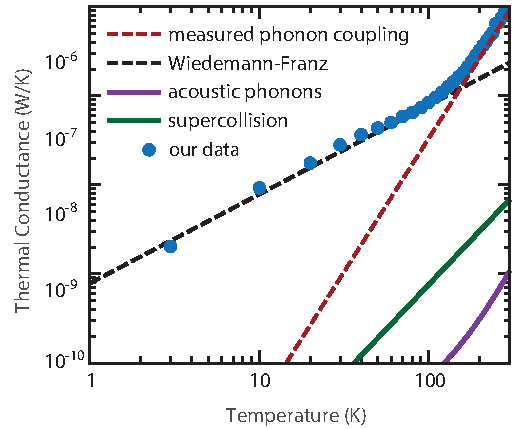
\includegraphics[width=3.5in]{EPh_v2.pdf}
\caption{Comparison of the measured thermal conductance to the heat transfer to phonons due to electron-phonon coupling. Data (blue diamonds) from Sample S1 at charge carrier density of 3.3 $\times 10^{11}$/cm$^2$. Red solid and green dashed lines are the expected thermal conductance of heat transfer from electrons to phonons.}
\label{figsEPh}
\end{figure}

\section{Measuring Thermal Conductivity}
In the diffusion-limited regime, we extract the electronic thermal conductivity $\kappa_{\mathrm{e}}$ as follows.    This is detailed in \cite{fong} and we review the basic calculation for clarity.   The total power dissipated, $P$, is given by \begin{equation}
P = \frac{J^2}{\sigma} LW = \mathcal{P}LW  \label{eqp2}
\end{equation}
where $L$ is the length of the sample in the direction of current flow,  $W$ is the width in the perpendicular direction and $\mathcal{P}$ is the local power dissipated.  Because this calculation is done in linear response, and the external heat baths on either side of the sample are at the same temperature,  the contributions to power dissipated $\sim \kappa (\Delta T)^2$ do not enter so long as $\Delta T \sim J^2$ is  small.   This is an appropriate assumption in the regime of linear response, where $J$ is treated as a perturbatively small parameter.    Fig. \ref{figs4} shows our experiment is in this regime.

Let us now determine the change in the temperature profile.   For simplicity we assume that the graphene sample is homogeneous, that the approximately uniform electrical current is given by \begin{equation}
J = -\sigma \frac{\mathrm{d}V}{\mathrm{d}x} - \alpha \frac{\mathrm{d}T}{\mathrm{d}x},  \label{S7}
\end{equation}
and that the heat current is given by \begin{equation}
Q = -\alpha T\frac{\mathrm{d}V}{\mathrm{d}x} - \bar\kappa_{\mathrm{e}} \frac{\mathrm{d}T}{\mathrm{d}x},  \label{S8}
\end{equation}
where \begin{equation}
\bar\kappa_{\mathrm{e}} \equiv \kappa_{\mathrm{e}} + \frac{T\alpha^2}{\sigma} = \kappa_{\mathrm{e}}(1+ZT).
\end{equation}
In the latter equation,  $ZT$ is the thermoelectric coefficient of merit.    As $\alpha \approx 0$ at the CNP,  we expect $ZT\approx 0$,  and that $\bar\kappa_{\mathrm{e}}\approx \kappa_{\mathrm{e}}$. 

 $\mathrm{d}T/\mathrm{d}x$ is the temperature gradient in the sample,  and $-\mathrm{d}V/\mathrm{d}x$ is the electric field in the sample.  $\alpha/\sigma$ is the Seebeck coefficient.  We assume that the response of graphene is dominated only by the changes in voltage $V$ and temperature $T$ to a uniform current density $J$, which is applied externally.  We also assume that deviations from constant $V$ and $T$ are small, so that the linear response theory is valid.  Joule heating leads to the following equations: \begin{subequations}\begin{align}
0 &= \frac{\mathrm{d}J}{\mathrm{d}x}, \\
\mathcal{P} = \frac{J^2}{\sigma} &=  \frac{\mathrm{d}Q}{\mathrm{d}x},
\end{align}\end{subequations}which can be combined to obtain \begin{equation}
\mathcal{P} = -\kappa_{\mathrm{e}} \frac{\mathrm{d}^2 T}{\mathrm{d}x^2},
\end{equation}
assuming that $\kappa_{\mathrm{e}}$ is approximately homogeneous throughout the sample.  


 \begin{figure}
 \centering
\includegraphics[width=3.5in]{SM_V2-08-eps-converted-to.pdf}
\caption{Cartoon illustrating the non-uniform temperature profile within the graphene-hBN stack during Joule heating in the diffusion-limited regime.}
\label{figs7}
\end{figure}

The contacts in our experiment are held at the same temperature $T$.   Thus, writing \begin{equation}
T(x) = T_{\mathrm{e}} + \Delta T(x),
\end{equation}we find that \begin{equation}
\Delta T(x) = \frac{\mathcal{P}}{2\kappa_{\mathrm{e}}}x(L-x).  
\end{equation}
The average temperature change in the sample, which is directly measured through JNT, is \begin{equation}
\langle \Delta T\rangle = \int\limits_0^L \frac{\mathrm{d}x}{L}\; \Delta T(x)  = \frac{\mathcal{P}L^2}{12\kappa_{\mathrm{e}}}.  \label{eqp3}
\end{equation}
This non-uniform temperature profile is illustrated in Fig. \ref{figs7}.   Combining Eqs. (\ref{eqp1}), (\ref{eqp2}) and (\ref{eqp3}) we obtain \begin{equation}
G_{\mathrm{th}} = \frac{12L}{W} \kappa_{\mathrm{e}}.
\end{equation}

As we have pointed out in the main text,  our samples are not perfectly homogeneous, but have local fluctuations in the charge density.   Nevertheless, we do recover the WF law in the FL regime, suggesting that our measurement of $G_{\mathrm{th}}$ -- and thus $\kappa_{\mathrm{e}}$ -- using JNT, along with the above formalism, is valid.

\section{Bipolar Diffusion }
The bipolar diffusion effect occurs when different charge carriers of opposite sign move in the same direction under an applied temperature gradient. The thermal conductivity $\kappa$,  as defined in the main text in the absence of net electric current flow, is given in Ref. \cite{goldsmid}:
\begin{equation}
\kappa \equiv \left(\bar\kappa_{\mathrm{e}} - \frac{T\alpha_{\mathrm{e}}^2}{\sigma_{\mathrm{e}}}\right) + \left(\bar\kappa_{\mathrm{h}} - \frac{T\alpha_{\mathrm{h}}^2}{\sigma_{\mathrm{h}}}\right) + \frac{T\sigma_{\mathrm{e}}\sigma_{\mathrm{h}}}{\sigma_{\mathrm{e}}+\sigma_{\mathrm{h}}}\left(\frac{\alpha_{\mathrm{e}}}{\sigma_{\mathrm{e}}}-\frac{\alpha_{\mathrm{h}}}{\sigma_{\mathrm{h}}}\right)^2  \label{bdformula}
\end{equation}
The first two terms in the above equations are the thermal conductivity of electrons and holes respectively. The third term is the bipolar diffusion term, and accounts for the possibility of electrons and holes flowing in the same direction.


Bipolar diffusion has been used to explain the thermal conductivity of narrow gap semiconductors, such as bismuth telluride, when the chemical potential is close to the midgap. Estimates of the Lorenz ratio in bismuth telluride have been reported as high as 7.2 $\mathcal{L}_0$  in Ref. \cite{GOLDSMID:1956cs}.   In graphene, the two types of charge carriers correspond to above/below the Dirac point.  To use the formula (\ref{bdformula}) requires the assumption that interactions between electrons and holes are negligible. If this is the case, it is reasonable to employ kinetic theory to estimate $\sigma_{\mathrm{e,h}}$, $\alpha_{\mathrm{e,h}}$ and $\bar\kappa_{\mathrm{e,h}}$.  This was shown in Ref. \cite{yoshino} and we state the formalism here for completeness.

Employing the ultrarelativistic band structure of graphene near the CNP, the transport coefficients are given by:
 \begin{subequations}\begin{align}
\sigma_{\mathrm{e}} &= \int \frac{\mathrm{d}^2\mathbf{k}}{2\pi^2} \tau_{\mathrm{e}}(\mathbf{k})  v_{\mathrm{F}}^2 \mathcal{F}\left(\frac{\hbar v_{\mathrm{F}} k \pm \mu}{k_{\mathrm{B}}T}\right), \\
\alpha_{\mathrm{e}} &= \pm \int \frac{\mathrm{d}^2\mathbf{k}}{2\pi^2} \tau_{\mathrm{e}}(\mathbf{k}) (\hbar v_{\mathrm{F}} k \pm \mu) v_{\mathrm{F}}^2 \mathcal{F}\left(\frac{\hbar v_{\mathrm{F}} k \pm \mu}{k_{\mathrm{B}}T}\right), \\
\bar\kappa_{\mathrm{e}} &= \int \frac{\mathrm{d}^2\mathbf{k}}{2\pi^2} \tau_{\mathrm{e}}(\mathbf{k}) (\hbar v_{\mathrm{F}} k \pm \mu)^2 v_{\mathrm{F}}^2\mathcal{F}\left(\frac{\hbar v_{\mathrm{F}} k \pm \mu}{k_{\mathrm{B}}T}\right),
\end{align}\end{subequations}
where $\tau_{\mathrm{e,h}}$ are suitably defined energy relaxation times for electrons and holes, we use a $\pm$ sign for electrons/holes,  and \begin{equation}
\mathcal{F}(x) \equiv \frac{1}{k_{\mathrm{B}}T} \frac{\mathrm{e}^x}{(1+\mathrm{e}^x)^2}.
\end{equation}

\begin{figure}
\centering
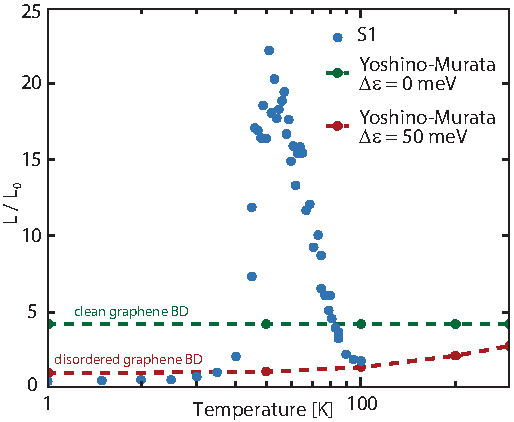
\includegraphics[width=3.5in]{LorenzComparison.pdf}
\caption{Comparison of the Lorenz ratio in graphene between bipolar diffusion theory \cite{yoshino} and our experimental data.   The sharp temperature dependence of $\mathcal{L}$ is  inconsistent with bipolar diffusion (see green dashed lines).  This sharp behavior is predicted in hydrodynamics \cite{Lucas:2015sya}.}
\label{FigLorenzComparison}
\end{figure}

Given a choice of $\tau$,  it is straightforward to numerically integrate these equations.  This was done in Ref. \cite{yoshino} for some choices of $\tau$; we have checked additional choices.   We compare the result of this two-band formalism at the CNP, to the same data for S1 used in Figure 3 of the main text.    We can rule out the canonical bipolar diffusion (BD) explanation of our data for the following reasons: 

\noindent (1) The BD theory predicts that   $\mathcal{L}/\mathcal{L}_{\mathrm{WF}}$ is independent of temperature at the CNP in a clean sample.    Adding disorder only adds a very weak temperature dependence \cite{yoshino}.  This is in stark contrast to our data -- see Figure \ref{FigLorenzComparison}.   Hydrodynamic models do predict a sharp temperature dependence in $\mathcal{L}$ \cite{Lucas:2015sya}.
\\\\
\noindent (2) Simple models of BD in the presence of charge puddles with local chemical potential fluctuations of 50 meV or higher predict factor of 2 violations of the WF law \cite{yoshino}, and a weak dependence of $\mathcal{L}$ on disorder, compared to hydrodynamics.   In contrast we see a sharp dependence on disorder, comparing our three samples (Figure 3 of the main text).   In samples where chemical potential fluctuations are comparable to 50 meV, the WF law is obeyed to within 40\% \cite{fong}.
\\\\
\noindent (3) Working under the theory of \cite{sarma2009}, $\tau(\mathbf{k}) \sim |\mathbf{k}|$, and hence the maximal Lorenz ratio $\mathcal{L}/\mathcal{L}_{\mathrm{WF}}\approx 4$ \cite{yoshino}  -- well below to our experimental observation of $\mathcal{L}/\mathcal{L}_{\mathrm{WF}}\approx 22$.
\\\\
\noindent (4) The BD theory of \cite{yoshino} predicts $\mathcal{L}/\mathcal{L}_{\mathrm{WF}} \gtrsim 0.8$ under all conditions.   Hydrodynamics predicts that this ratio can become arbitrarily small in a clean sample, and we have indeed observed $\mathcal{L}/\mathcal{L}_{\mathrm{WF}} \sim 1/3$ at finite density in the DF in sample S1, only consistent with hydrodynamics.



\chapter{Appendix for Chapter 9}

\section{Thermodynamics}\label{appthermo}
In this appendix and in every subsequent appendix, we will work in units where $\hbar=k_{\mathrm{B}}=v_{\mathrm{F}}=e=1$.     It is straightforward using dimensional analysis to restore these units.  

We consider the equations of state of the relativistic plasma in a relativistic strongly interacting fluid in $d=2$.    Without specific microscopic details, these are very general facts about relativistic plasmas without an intrinsic mass scale (or gap).  The discussion generalizes straightforwardly to other $d$.    The only relevant energy scales are the temperature $T$ and the chemical potential $\mu$.     We have the general Gibbs-Duhem relation:\begin{equation} \label{duhem}
\epsilon + P = \mu n + Ts,
\end{equation}where $\epsilon$ is the energy density, $P$ is the pressure, $s$ is the entropy density and $n$ is the charge density ($n=0$ at the particle-hole symmetric Dirac point).   In a relativistic fluid, \begin{equation}
P  = T^3 \mathcal{F}\left(\frac{\mu}{T}\right)
\end{equation}for some dimensionless function $\mathcal{F}$.  Thermodynamic identities imply that \begin{subequations} \label{qmu}\begin{align}
n &= \frac{\partial P}{\partial \mu} = T^2 \mathcal{F}^\prime \left(\frac{\mu}{T}\right) \\
s &= \frac{\partial P}{\partial T} = 3T^2 \mathcal{F} -  \mu T\mathcal{F}^\prime \left(\frac{\mu}{T}\right) = \frac{3P - \mu n }{T}.
\end{align}\end{subequations}Combining (\ref{duhem}) and (\ref{qmu}) we obtain \begin{equation}
\epsilon = 2P.
\end{equation}

The hydrodynamic description is only sensible for $\mu \ll T$ -- for $\mu \gg T$ the standard Fermi liquid description applies.   Furthermore, the equations of state of the Dirac fluid are charge conjugation symmetric, implying that $\mathcal{F}$ is an even function of $\mu$.   So we Taylor expand: \begin{equation}
\mathcal{F}\left(\frac{\mu}{T}\right) \approx \frac{C_0}{3} + \frac{C_2}{2} \left(\frac{\mu}{T}\right)^2 +  \frac{C_4}{4} \left(\frac{\mu}{T}\right)^4.  \label{feq}
\end{equation} Using (\ref{qmu}): \begin{subequations}\begin{align}
n &= C_2 \mu T + C_4 \frac{\mu^3}{T}, \\
s &= C_0T^2 + \frac{C_2 \mu^2}{2} - \frac{C_4 \mu^4}{4T^2} .
\end{align}\end{subequations}
We also require that $C_0,C_2\ge 0$, so that $s\ge 0$ and that $n/\mu$ is positive as $\mu\rightarrow 0$, as it should be.

%In $d\ne 2$, assuming $B=0$,  a straightforward calculation analogous to the above gives $\epsilon=dP$.   This implies that the stress-energy tensor is traceless with respect to the Minkowski metric in every dimension.   This is a general consequence of relativistic scale invariance.

\subsection{Thermodynamics of Disordered Fluids}
Already at this point we can make interesting predictions about the thermodynamics of the strongly interacting hydrodynamic regime in graphene.   For concreteness, let us suppose that the background chemical potential is \begin{equation}
\mu_0(\mathbf{x}) = \bar\mu_0 + \hat\mu(\mathbf{x}),
\end{equation}
with $\bar\mu_0$ a constant and $\hat\mu$ a zero-mean random function;  for simplicity, suppose that $\hat\mu$ is evenly distributed about zero, and has a disorder correlation length of $\xi\gtrsim l_{\mathrm{ee}}$, so that the hydrodynamic description applies.   In this case, spatially averaging over $\mu_0$, we find \begin{equation}
\langle \epsilon\rangle = \frac{2C_0}{3}T^3  + C_2T\left(\bar\mu_0^2+\left\langle \hat\mu^2\right\rangle \right) + \frac{C_4}{2}\left(\bar\mu_0^4 + 6\bar\mu_0^2\left\langle \hat\mu^2\right\rangle + \left\langle \hat\mu^4\right\rangle\right) + \cdots.
\end{equation}
The $\cdots$ denotes higher order terms in the equation of state that we have neglected.  A similar expression can be found for the charge density: \begin{equation}
\langle n\rangle = C_2 T \bar\mu_0 + \frac{3C_4}{T}\bar\mu_0 \left\langle \hat\mu^2\right\rangle + \cdots.
\end{equation}

Let us focus on a clean limit where $\hat\mu$ is very small relative to $T$.    Let us also assume that we are close to the Dirac point, so that only $C_0$ and $C_2$ terms need to be kept.   Thermodynamics then gives tight constraints on the behavior of measurable quantities: specific heat and compressibility,  in an experimentally testable regime, due to the ability to easily tune both $T$ and $\bar\mu_0$ (the average charge density) experimentally.  In the limit above, the (spatially averaged) compressibility $\mathcal{K}$ is \begin{equation}
\frac{1}{\mathcal{K}} = \frac{\partial \langle n\rangle}{\partial \mu}  = C_2T.
\end{equation}
where as before, we use $\langle\cdots\rangle$ to denote a uniform spatial average.    Note that the independence of $\mathcal{K}$ to $\bar\mu_0$ and $\hat\mu$ is simply a consequence of the fact that we did not expand (\ref{feq}) to quartic order.  The spatially averaged specific heat \begin{equation}
 c = \frac{\partial \langle \epsilon\rangle}{\partial T} = 2C_0T^2 + C_2\left(\bar\mu_0^2+\left\langle \hat\mu^2\right\rangle\right).
\end{equation}

The experimental consequence of this result is as follows.   Very close to the Dirac point, we expect that $\mathcal{K}$ is approximately constant.   Restoring all dimensional prefactors, we can therefore set \begin{equation}
C_2 \approx \frac{(\hbar v_{\mathrm{F}})^2}{\mathcal{K}k_{\mathrm{B}}T}
\end{equation}
and re-write \begin{equation}
c \approx 2C_0 \frac{k_{\mathrm{B}}^3T^2}{(\hbar v_{\mathrm{F}})^2} + 2\frac{\bar\mu_0^2+\left\langle \hat\mu^2\right\rangle}{\mathcal{K}T} \approx 2C_0 \frac{k_{\mathrm{B}}^3T^2}{(\hbar v_{\mathrm{F}})^2} + 2\frac{\left\langle \hat\mu^2\right\rangle}{\mathcal{K}T} + \frac{2\mathcal{K}  n^2}{T} .
\end{equation}
We thus see that the quadratic dependence in $c(n)$ gives us an independent measurement of $\mathcal{K}$ through a measurement of the heat capacity.   In principle, a quadratic polynomial fit to $c(n)$ thus determines both $\mathcal{K}$ and $C_0$,  up to the residual effects of disorder, which will lead to an overestimate of $C_0$.   Repeating measurements of $\mathcal{K}$ directly, as well as $c(n)$ at different $T$,  provide non-trivial checks on the above theory.   It is important to note that this argument does \emph{not} rely on the validity of hydrodynamics, only that graphene is gapless, $\bar\mu_0 \ll T$, and that $\hat\mu$ is very small.   Of these three requirements, the last poses the biggest experimental hurdle.


In the above argument, there is no reason a priori why to truncate the Taylor expansion to neglect $C_4$ and higher order corrections, beyond appealing to the weak disorder limit.   In particular, inclusion of $C_4$ complicates our ability to obtain an accurate measure of $\bar\mu_0$ from $n$.    The argument above is simply meant to give a flavor for the constraints on measurable quantities imposed by scale invariant thermodynamics.   A more systematic treatment is likely necessary to make quantitative contact with future experiments.

\section{Rescaling Symmetries of dc Transport}\label{apprescale}
Solutions to (\ref{bigeq}) are invariant, up to global rescalings, under certain rescalings of the linearized hydrodynamic equations of motion.   These symmetries are, assuming $\lambda>0$ is a constant scaling parameter:  
\begin{subequations}\begin{align}
\eta &\rightarrow \lambda^2 \eta, \;\; x \rightarrow \lambda x; \\
\eta &\rightarrow \lambda \eta, \;\; \sigma \rightarrow \lambda \sigma, \;\; \alpha \rightarrow \lambda\alpha, \;\; \kappa \rightarrow \lambda\kappa, \;\; P \rightarrow \lambda P; \\
\alpha &\rightarrow \lambda \alpha, \;\; \kappa \rightarrow \lambda^{2}\kappa, \;\; \eta \rightarrow \lambda^{-2} \eta, \;\;\; \mu_0 \rightarrow \lambda \mu_0, \;\; C_2 \rightarrow \lambda^{-2}C_2,\;\; C_4 \rightarrow \lambda^{-4}C_4,\;\; \mathrm{etc.}; \\
\alpha &\rightarrow \lambda \alpha, \;\; \kappa \rightarrow \lambda\kappa, \;\; \sigma \rightarrow \lambda\sigma, \;\; \eta \rightarrow \lambda^{-1} \eta.
\end{align}\end{subequations}
Everything not listed is invariant.  $\zeta$ and $\eta$ have the same scalings, as do $\sigma$ and $\sigma_{\textsc{q}}$, and so we have only listed some of these parameters.     

These rescalings are useful to help us compare simulations to experimental data from graphene.  The latter three rescalings can be used to help fix the overall magnitude of $\kappa$ and $\sigma$, as well as the values of $n$, as measured in experiment.    These are exactly analogous to the symmetries of the Navier-Stokes equation, which allow us to reduce all such hydrodynamic problems to a universal equation, up to a single dimensionless parameter.   \cite{Crossno1058} neither measured the viscosity directly nor the charge puddle size, and the first scaling above implies that we cannot determine viscosity alone.  So, as mentioned in the main text, we assume that $\xi = l_{\mathrm{ee}}$,  the shortest possibile value of $\xi$ for which hydrodynamics seems sensible.   

\section{Weak Disorder}\label{appmom}
Many analytic results can be obtained in the limit where the disorder strength is ``small".   We provide detailed derivations of all such results in this appendix.    We introduce disorder as in (\ref{pertlimit}).    Below we denote $n_0 = n(\bar\mu_0)$, etc.

The perturbative solution is found exactly as was done in \cite{Lucas:2015lna}:   we split the velocity field into a constant piece $\bar v_i \sim u^{-2}$, and a fluctuating zero-mean piece $\hat v_i \sim u^{-1}$;  similarly, $ \mu \sim  T \sim u^{-1}$.   It proves convenient to work in Fourier space.   At $\mathrm{O}(u^{-1})$, the momentum conservation equation becomes \begin{equation}
-\mathrm{i}k_i \left(n_0  \mu(\mathbf{k})+s_0 T(\mathbf{k})\right) = \eta_0 k^2  \hat v_i(\mathbf{k}) + \zeta_0 k_ik_j  \hat v_j(\mathbf{k}),
\end{equation} 
and the conservation laws become (at the same order) \begin{subequations}\begin{align}
0 &= \mathrm{i}k_i \left(\hat n(\mathbf{k})  \bar v_i + n_0  \hat v_i(\mathbf{k})\right)+ \sigma_{\textsc{q}0} k^2 \left( \mu(\mathbf{k}) - \frac{\mu_0}{T_0} T(\mathbf{k})\right), \\
0 &= \mathrm{i}k_i T_0 \left(\hat s(\mathbf{k})  \bar v_i + s_0  \hat v_i(\mathbf{k})\right) -\mu_0\sigma_{\textsc{q}0} k^2 \left( \mu(\mathbf{k}) - \frac{\mu_0}{T_0} T(\mathbf{k})\right).
\end{align}\end{subequations}
Combining these equations we obtain expressions for $ T$, $ \mu$ and $k_i  \hat v_i$: \begin{subequations}\begin{align}
k_i  \hat v_i(\mathbf{k}) &= -\frac{\mu_0 \hat n(\mathbf{k}) + T_0\hat s(\mathbf{k})}{\mu_0 n_0 + T_0s_0} k_i  \bar v_i, \\
 T(\mathbf{k}) &= -\frac{\mathrm{i}k_i  \bar v_i}{\sigma_{\textsc{q}0}k^2(\epsilon_0+P_0)^2}\left(\sigma_{\textsc{q}0}k^2 (\eta_0+\zeta_0)(\mu_0 \hat n + T_0\hat s)T_0 - T_0n_0(T_0s_0\hat n-T_0n_0\hat s)\right), \\
 \mu(\mathbf{k}) &= -\frac{\mathrm{i}k_i  \bar v_i}{\sigma_{\textsc{q}0}k^2(\epsilon_0+P_0)^2}\left(\sigma_{\textsc{q}0}k^2 (\eta_0+\zeta_0)(\mu_0 \hat n + T_0\hat s)\mu_0 + T_0s_0(T_0s_0\hat n-T_0n_0\hat s)\right).
\end{align}\end{subequations}
Spatially averaging over the momentum conservation equation at $\mathrm{O}(u^0)$, and defining: 
\begin{equation}
(\epsilon+P)\tau^{-1}_{ij}  \bar v_j \equiv  \sum_{\mathbf{k}} \mathrm{i}k_i \left[\hat n(-\mathbf{k})  \mu(\mathbf{k}) + \hat s(-\mathbf{k})  T(\mathbf{k})\right],
\end{equation}
we find that \begin{equation}
\tau^{-1}_{ij} = \sum_{\mathbf{k}} \frac{k_ik_j}{k^2} \frac{\left| T_0s_0 \hat n(\mathbf{k}) - T_0n_0 \hat s(\mathbf{k})\right|^2 + \sigma_{\textsc{q}0}k^2 (\eta_0+\zeta_0) \left|\mu_0 \hat n(\mathbf{k}) + T_0\hat s(\mathbf{k})\right|^2}{\sigma_{\textsc{q}0}(\epsilon_0+P_0)^3}   \label{taueq1}
\end{equation}and that the spatially averaged momentum equation reduces to \begin{equation}
0  = n_0  E_i + T_0s_0  \zeta_i -(\epsilon_0+P_0)\tau^{-1}_{ij} \bar v_j .  \label{hydrocpeq}
\end{equation}
In this equation, we have used the fact that $ J_i \approx n \bar v_i$ at leading order in perturbation theory.   The resulting transport coefficients are analogous to (\ref{drudeeq}): \begin{subequations}\begin{align}
\sigma_{ij} &= \frac{n_0^2}{\epsilon_0+P_0}  \tau_{ij}, \\
\bar\alpha_{ij} = \alpha_{ij} &=  \frac{n_0s_0}{\epsilon_0+P_0}\tau_{ij}, \\
\bar\kappa_{ij} &= \frac{Ts_0^2}{\epsilon_0+P_0}\tau_{ij}.
\end{align}\end{subequations}In the expression for $\sigma$, we have not included a $\sigma_{\textsc{q}0}$ contribution, as was done in \cite{hkms}, as this is a subleading order in perturbation theory.

Using our Taylor expanded equations of state for the fluid and assuming $C_4=0$, since \begin{equation}
\hat s(\mathbf{k}) \approx C_2 \mu_0 \hat\mu(\mathbf{k}) = \frac{\mu_0}{T_0}\hat n(\mathbf{k}),
\end{equation}we can simplify (\ref{taueq1}) to \begin{equation}
\tau^{-1}_{ij} = \sum_{\mathbf{k}} \frac{k_ik_j}{k^2} \frac{\left(T_0s_0-\mu_0n_0\right)^2 +4 \sigma_{\textsc{q}0}k^2 (\eta_0+\zeta_0) \mu_0^2 }{\sigma_{\textsc{q}0}(\epsilon_0+P_0)^3}\left|\hat n(\mathbf{k})\right|^2
\end{equation}
Similar results were presented (in a different format) in \cite{Davison:2013txa}, though the practical consequences of this formula, as discussed in the main text, have not previously been understood.


We cannot take the naive limit where $\sigma_{\textsc{q}0}\sim u^{-2}$ in order to recover (\ref{hkmseq}) in full generality.     The simplest way to see that something goes wrong is to study $\bar\kappa$ near $\bar\mu_0=0$ (more precisely, $\bar\mu_0\sim u$):  if $\sigma_{\textsc{q}} \sim u^{-2}$  we find that $\tau \sim u^{-4}$, and this implies that the heat current (and thus $\bar\kappa$) would be parametrically larger than anticipated.   Thus our perturbative scaling breaks down.   The breakdown of the perturbative theory for $u\sim \bar\mu_0$ was also advocated in \cite{Lucas:2015lna}.  
 
 Although we have argued there are problems in principle with (\ref{hkmseq}) when $\bar\mu_0 \sim u$, even when $u$ is perturbatively small, in practice  the mean-field model of \cite{hkms} can be quite good in practice near $\bar\mu_0\sim u$, as shown in Figure \ref{viscfig}.   Note that it is also important that $C_0 T^2 \gg C_2 u^2$ -- when this limit is violated, we see substantial deviations from (\ref{hkmseq}) at all $\bar\mu_0$, as shown in Figure \ref{viscfig}.  This may be a consequence of our assumption that $\sigma_{\textsc{q}}$ is independent of $\mu_0$.

 
 

\section{Equations of State of the Dirac Fluid}\label{apprun}
The thermodynamics of graphene is similar to that presented in Appendix \ref{appthermo}, with some minor differences.    Perturbative computations and renormalization group arguments, valid as $T\rightarrow 0$, give \cite{vafek, schmalian} \begin{subequations}\label{cb}\begin{align}
C_0 &= \frac{9\mzeta(3)}{\mpi} \left(\frac{\alpha_{\mathrm{eff}}}{\alpha_0}\right)^2 \approx 3.44 \left(\frac{\alpha}{\alpha_0}\right)^2, \\
C_2 &= \frac{4\log 2}{\mpi}  \left(\frac{\alpha_{\mathrm{eff}}}{\alpha_0}\right)^2 \approx 0.88 \left(\frac{\alpha}{\alpha_0}\right)^2.
\end{align}\end{subequations}
(\ref{cb}) can be derived by computing the thermodynamics of 2 species of non-interacting Dirac fermions, with Coulomb interactions leading to a logarithmically increasing Fermi velocity \cite{vafek, schmalian}.    As $\alpha_{\mathrm{eff}}(T)$ is not a constant, this implies that the entropy has an additional contribution related to the logarithmic $T$ dependence of $C_{0,2}(\alpha_{\mathrm{eff}})$.   Assuming $C_0$ and $C_2$ above, and assuming $C_4=0$ for simplicity as its value for free fermions is quite small \cite{muller1}, we find: \begin{equation}
   s = C_0 T^2 \left[1 + \frac{\alpha_{\mathrm{eff}}}{6}\right]+ \frac{C_2}{2}\mu^2\left[1 + \frac{\alpha_{\mathrm{eff}}}{2}\right]  \label{saeff}
   \end{equation}
This equation directly implies $\epsilon>2P$.   Using the estimate $\alpha_{\mathrm{eff}}\sim 0.25$ from above, we see that the corrections to $s$ (and $\epsilon$) are rather minor ($<10$\%);  $n$ is unchanged.   In fact,  (\ref{saeff}) is not quite right: the computation of (\ref{cb}) is only a leading order perturbative computation:  there are corrections to (\ref{cb}) at higher orders in $\log \alpha_{\mathrm{eff}}$.    Nonetheless, our general conclusion that $\epsilon>2P$ is possible in graphene continues to hold, given any logarithmic running of the Fermi velocity.

As noted above, these theoretical computations of the thermodynamic coefficients in graphene are all perturbative computations in $\alpha_{\mathrm{eff}}$,  yet we only expect $\alpha_{\mathrm{eff}}/\alpha_0\sim 0.5$:  there is no reason to expect that higher order corrections, which can be as large as $\sim \log \alpha_{\mathrm{eff}}$, are negligible.  More sensitive experiments may find discrepancies with Lorentz invariant hydrodynamics, associated with these peculiar properties of the Dirac fluid.   Similar logarithms can appear in $\sigma_{\textsc{q}}$ \cite{muller2} and $\eta$ \cite{muller2009}, and in both cases, for the reasons above, we neglect these logarithms and use the theory of Section \ref{sechydro}.
   

\section{Numerical Methods}\label{appfin}
We solved the hydrodynamic equations (\ref{bigeq}) on a periodic domain of size $L\times L$, employing pseudospectral methods \cite{trefethen} using a basis of $N$ Fourier modes in each direction, with $25 \lesssim N \lesssim 43$.   For simplicity, we set $T_0=1$, as this can be restored straightforwardly by dimensional analysis.   Our numerical methods involves approximating continuous partial differential equations in the form \begin{equation}
\mathsf{L} \mathbf{u} = \mathbf{s}.
\end{equation}
 $\mathbf{u}$ contains the linear response fields $\mu$, $T$, $v_x$ and $v_y$, evaluated on a uniformly distributed discrete grid, and $\mathbf{s}$ contains the source terms, linear in $E_i$ and $\zeta_i$, evaluated at the same points.   $\mathsf{L}$ is a matrix with two zero eigenvectors, which correspond to constant shifts in $\mu$ and $T$ respectively.  We thus remove two rows of $\mathsf{L}$ and replace them with constraints that $\mu(\mathbf{0}) = T(\mathbf{0}) = 0$.  A simple matrix inversion thus gives $\mathbf{u} = \mathsf{L}^{-1}\mathbf{s}$.   Inverting this $(4N^2-2)\times (4N^2-2)$ matrix four times (once for sources $E_{x,y}$ and $\zeta_{x,y}$) limits the size of the domain we can analyze.   More complicated algorithms exist \cite{domaindec} to solve such problems but we did not find finite size effects to qualitatively alter our comparison to experimental data, as we discuss below.
 
As mentioned in the main text, our disorder realizations consisted of random sums of sine waves.  More precisely, \begin{equation}
\mu_0(\mathbf{x}) = \bar\mu_0 + \sum_{|n_x|,|n_y| \le k} \hat\mu_0(n_x,n_y) \sin\left(\phi_x + \frac{2n_x\mpi x}{k\xi}\right)\sin\left(\phi_y + \frac{2n_y\mpi y}{k\xi}\right)
\end{equation} 
with $\bar\mu_0$ a constant, $\hat\mu_0(n_x,n_y)$ uniformly distributed on $[-c,c]$ where $c=\sqrt{(2-\mdelta_{n_x,0}-\mdelta_{n_y,0})/2}$, and $\phi_{x,y}$ uniformly distributed on $[0,2\mpi)$.   The lack of heavy tails in $\hat\mu_0(n_x,n_y)$, perhaps associated with point-like impurities, is consistent with experiment \cite{yacoby2007}.  The form of $c$ is chosen so that we do not add random charge density bias to our disorder (as the zero mode has no amplitude), and so that all Fourier modes included at finite wave number have the same average amplitude.
 
 
\subsection{Finite Size Effects}
The first source of finite size effects is simply related to the fact that we only have a finite number of disorder modes.   Averaging over a large number of ensemble samples allows us to approximately, but not exactly, undo this effect:  see Figures \ref{finitesize2plot} and  \ref{finitesizeplot}.   In both cases,  we used $8k+3$ grid points in each direction for various $k$.   To the best of our knowledge, in all numerical simulations we have studied, it appears as though the result converges to a finite fixed answer as $k\rightarrow \infty$.  However, residual error from finite size effects may lead to some error in our estimation of the thermodynamic and hydrodynamic coefficients of the Dirac fluid in graphene.

\begin{figure}[t]
\centering
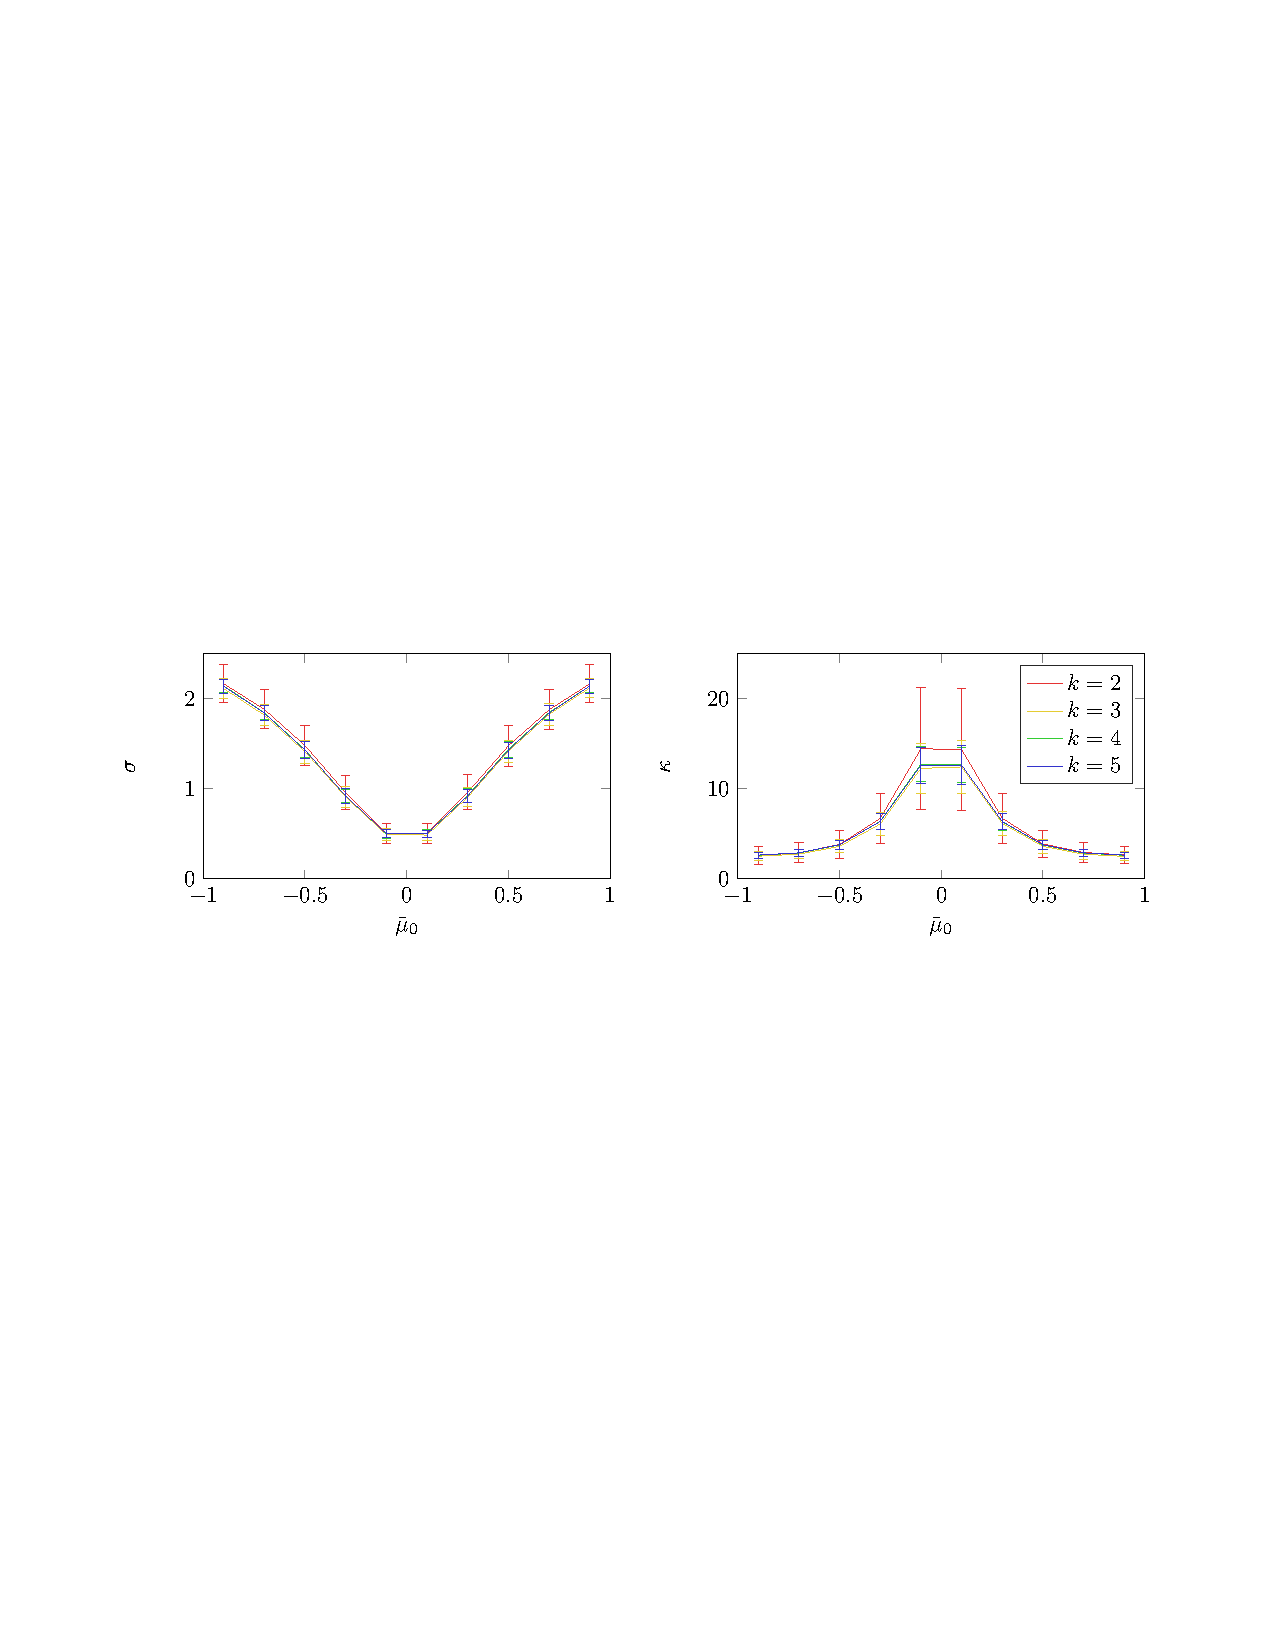
\includegraphics[width=6in]{finitesizeplot2.pdf}
\caption{Finite size effects with $u_0=0.3$, $C_0=3$, $C_2=1$, $\sigma_0=1$, $\eta_0=20$.  Numerical averages are performed over 100 disorder realizations.}
\label{finitesize2plot}
\end{figure}

\begin{figure}[t]
\centering
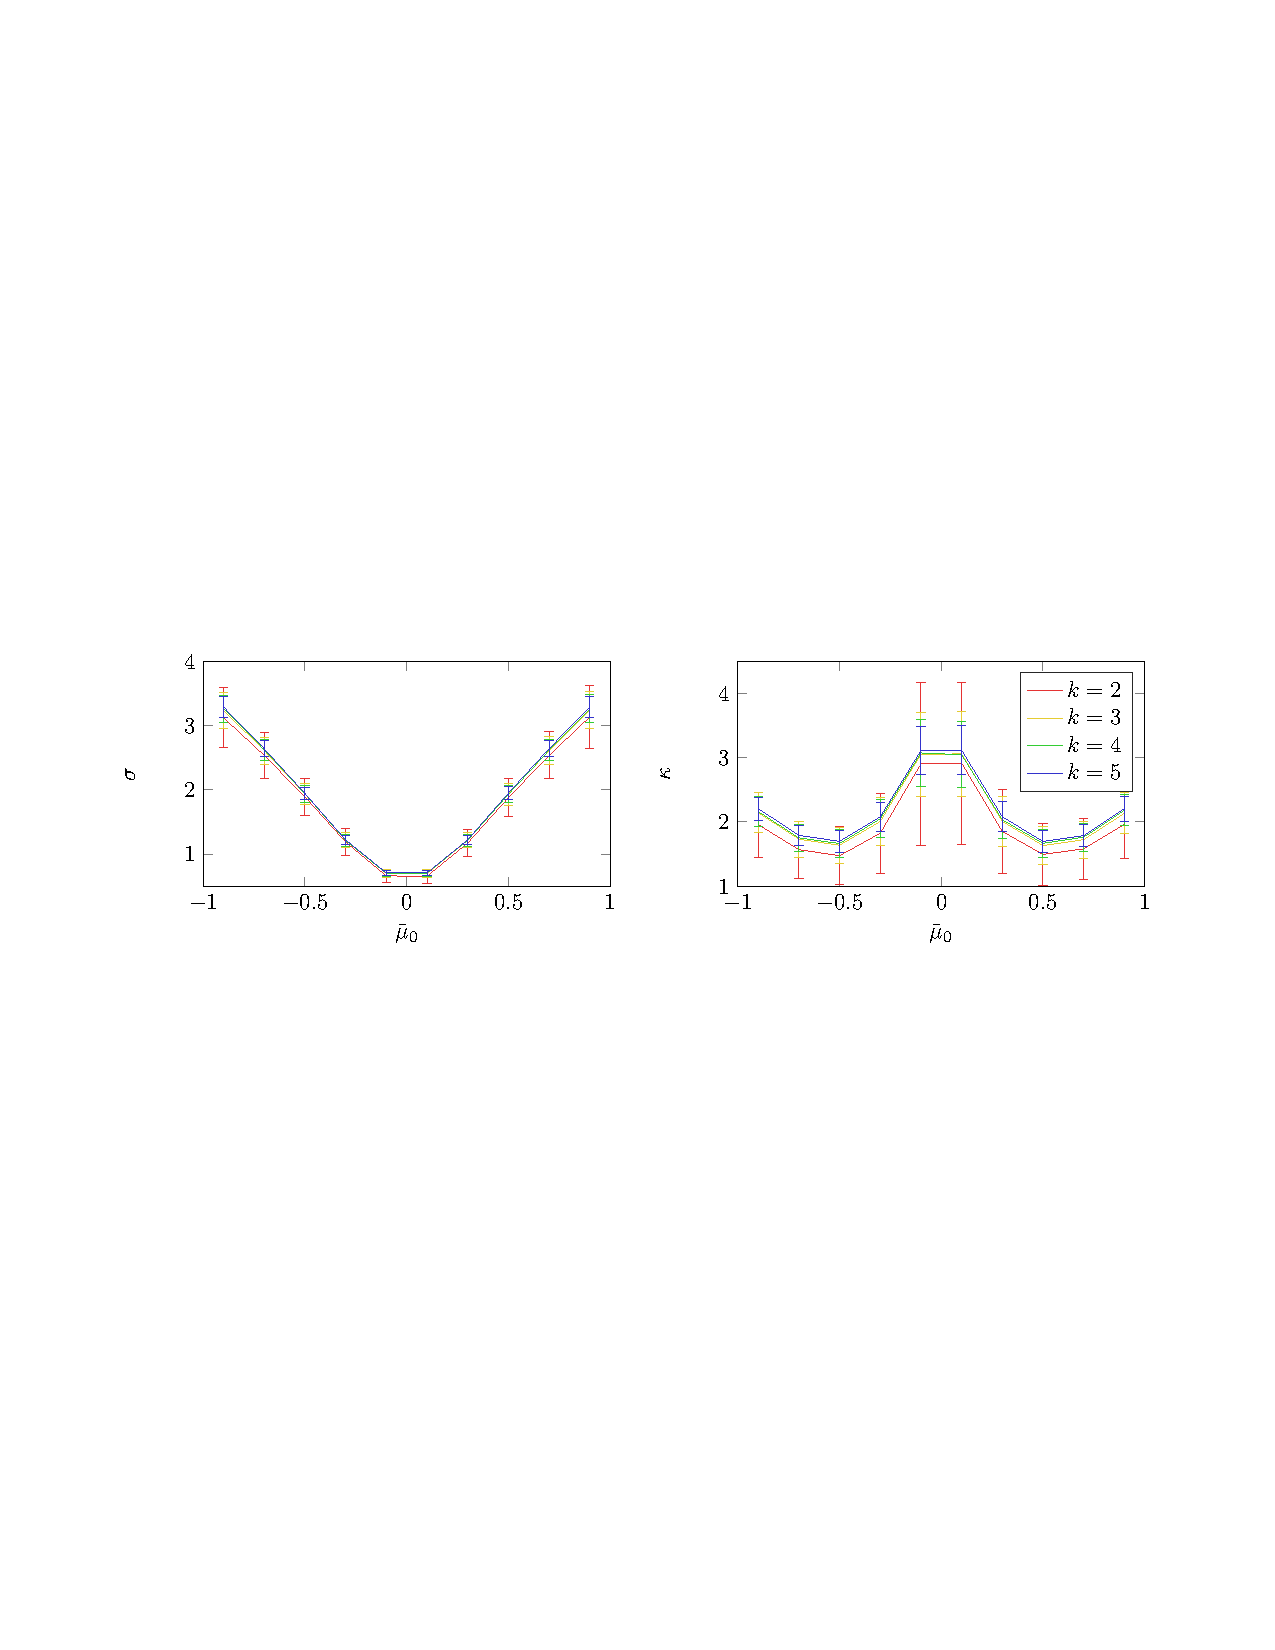
\includegraphics[width=6in]{finitesizeplot1.pdf}
\caption{Finite size effects with $u_0=0.3$, $C_0=1$, $C_2=1$, $\sigma_0=1$, $\eta_0=1$.  Numerical averages are performed over 100 disorder realizations.}
\label{finitesizeplot}
\end{figure}

%The finite size effect of a finite number of perturbative modes can be seen even in perturbation theory.   This is because in the formula for $\tau$, 

The other source of finite size effects is related to the finite number of grid points in our pseudospectral methods.   However, we expect standard exponential accuracy \cite{trefethen} in the number of grid points per $\xi$, which we have taken to be at least 10 in all figures in the main text.   Numerical evidence suggests that our spectral methods have converged to within about 0.1--1\% of the correct answer by this relatively small number of grid points per $\xi$, depending on the precise equations of state used.  In the case of the experimentally relevant parameters used in Figure \ref{mainfig}, we see exponential convergence of our spectral methods with increasing grid points, with numerical error of only 0.1\% by the time the number of grid points per $\xi$ is 11, as shown in Figure \ref{spectralfig}.     This spectral convergence is dramatically faster in the weak disorder limit.

\begin{figure}[t]
\centering
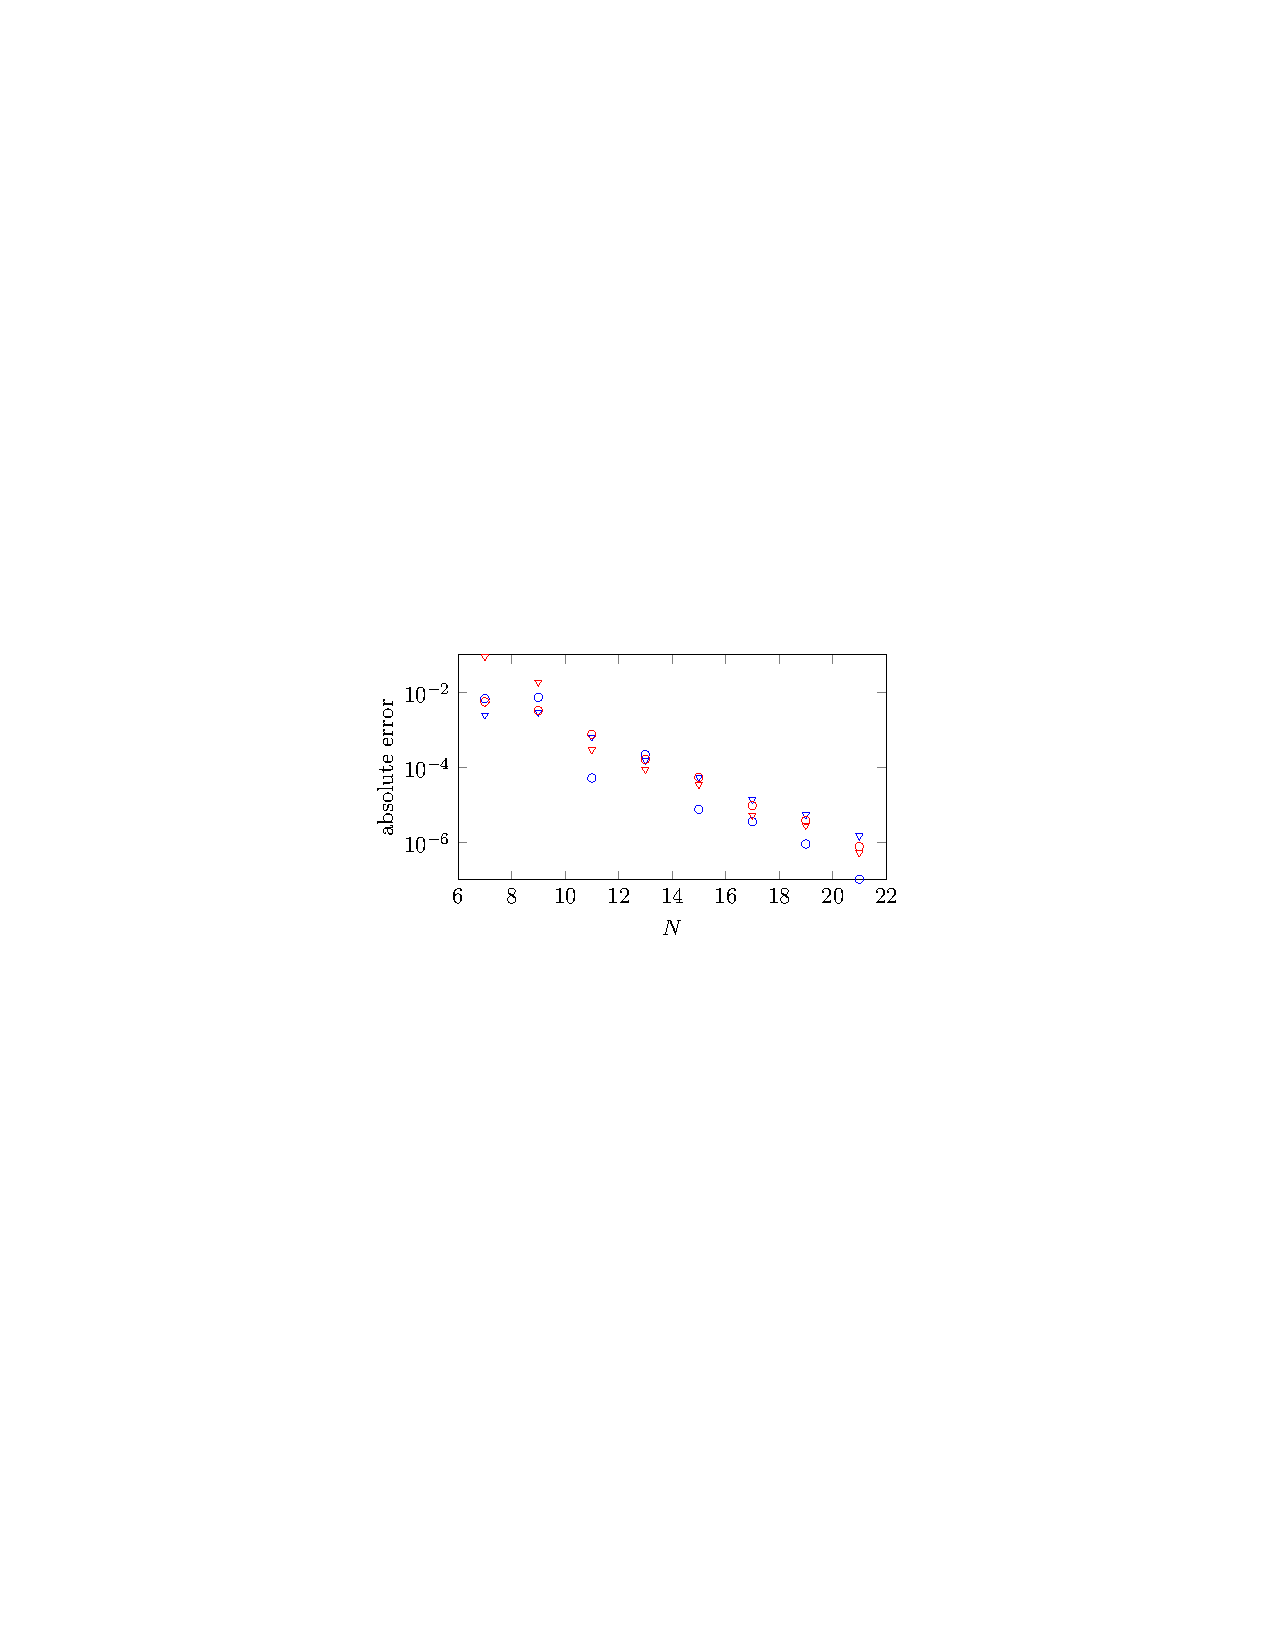
\includegraphics[width=3.3in]{spectralplot.pdf}
\caption{Exponential convergence of our pseudospectral code with an increasing number of grid points.  We computed $\kappa$ and $\sigma$ using our  code, employing the ``experimental" equations of state given in Figure \ref{mainfig},  and the disorder profile $\mu_0(x) = \bar\mu_0 + 2u\cos(2\mpi x/L)\cos(2\mpi y/L)$.   Red data points denote the error in $\kappa$, and blue points denote the error in $\sigma$.   Circles denote data at $\bar\mu_0 = 2u$, and triangles at $\bar\mu_0 = 0.4u$.  Absolute error is determined by (e.g.) $|\sigma(N)-\sigma(29)|/\sigma(29)$,  where we use the data points at $N=29$ as a reference point.}
\label{spectralfig}
\end{figure}

Methods are known to improve our simple algorithms, which can reduce both types of finite size effects discussed above.   Given the preliminary nature of the experiments to which we compare our simulations, we have found the numerical errors described above tolerable.

\subsection{Dimensional Analysis}
We have performed numerical computations in dimensionless units,   since we can trivially restore the units to our numerical results via dimensional analysis.   Setting $\hbar=k_{\mathrm{B}}=e=v_{\mathrm{F}}=T_0=1$ completely non-dimensionalizes the problem, while setting no dimensionless parameters to unity.    We can now trivially restore the units as follows:  \begin{subequations}\begin{align}
L &= \frac{\hbar v_{\mathrm{F}}}{k_{\mathrm{B}}T_0} \times L_{\mathrm{numerics}} \sim (100 \; \mathrm{nm}) \times L_{\mathrm{numerics}} \\
\mu &= k_{\mathrm{B}}T_0  \times \mu_{\mathrm{numerics}} \sim (5\; \mathrm{meV}) \times \mu_{\mathrm{numerics}}, \\
\sigma &= \frac{e^2}{\hbar}  \times \sigma_{\mathrm{numerics}} \sim (0.25\; \mathrm{k\Omega}^{-1}) \times \sigma_{\mathrm{numerics}}, \\
\alpha &= \frac{k_{\mathrm{B}}e}{\hbar}  \times \alpha_{\mathrm{numerics}} \sim \left(20\; \frac{\mathrm{nW}}{\mathrm{V}}\right) \times \alpha_{\mathrm{numerics}}, \\
\kappa &= \frac{k_{\mathrm{B}}^2T_0}{\hbar}  \times \kappa_{\mathrm{numerics}} \sim \left(0.1\; \frac{\mathrm{nW}}{\mathrm{K}}\right)  \times \kappa_{\mathrm{numerics}}.
\end{align}\end{subequations}
We have also noted the approximate scale of each important physical quantity in the problem for convenience.


\end{appendix}

\end{doublespace}

\pagestyle{fancy}
\renewcommand{\headrulewidth}{0pt}
\fancyhead{}

\fancyfoot{}
\fancyfoot[C] {\thepage}


\bibliographystyle{jhepsort}
\bibliography{RMPrefs}


\end{document}



% Figure 2


